% !TeX program = lualatex
\documentclass[fleqn]{NotesClass}

\strictpagecheck

%% Packages
\usepackage{tensor}
\usepackage{csquotes}
\usepackage{scalerel,stackengine}  % needed for d with slash
\usepackage{simpler-wick}
\usepackage{siunitx}
\usepackage{cancel}
\usepackage{ytableau}
\ytableausetup{centertableaux}

\usepackage{slashed}
\declareslashed{}{\not}{.1}{.5}{A}
\declareslashed{}{\not}{.05}{.5}{p}
\declareslashed{}{\not}{.1}{.5}{\partial}
\declareslashed{}{\not}{-.1}{.5}{a}
\declareslashed{}{\not}{.05}{.5}{D}

\let\widetildeOLD\widetilde
\AtBeginDocument{\let\widetilde\widetildeOLD}
\let\widehatOLD\widehat
\AtBeginDocument{\let\widehat\widehatOLD}

% Tikz stuff
\usepackage{tikz}
%\tikzset{>=latex}
% External
\usetikzlibrary{external}
\tikzexternalize[prefix=tikz-external/]
% Other libraries
\usetikzlibrary{decorations.markings, decorations.pathmorphing, patterns.meta, decorations.pathreplacing, calligraphy}

% Feynman diagram styles
\tikzset{scalar/.style={dashed}}
\tikzset{charged scalar/.style={dashed, postaction={decorate, decoration={markings, mark=at position #1 with {\arrow{Latex[width=1.5mm]}}}}}}
\tikzset{charged scalar/.default=0.5}
\tikzset{photon/.style={decoration={snake, amplitude=1.25, segment length=6}, decorate}}
\tikzset{electron/.style={postaction={decorate, decoration={markings, mark=at position #1 with {\arrow{Latex[width=1.5mm]}}}}}}
\tikzset{electron/.default=0.5}
\tikzset{positron/.style={postaction={decorate, decoration={markings, mark=at position #1 with {\arrowreversed{Latex[width=1.5mm]}}}}}}
\tikzset{positron/.default=0.5}
\tikzset{momentum injection/.style={->}}
\pgfdeclarepatternformonly{south west lines}{\pgfqpoint{-0pt}{-0pt}}{\pgfqpoint{3pt}{3pt}}{\pgfqpoint{3pt}{3pt}}{
    \pgfsetlinewidth{0.4pt}
    \pgfpathmoveto{\pgfqpoint{0pt}{0pt}}
    \pgfpathlineto{\pgfqpoint{3pt}{3pt}}
    \pgfpathmoveto{\pgfqpoint{2.8pt}{-.2pt}}
    \pgfpathlineto{\pgfqpoint{3.2pt}{.2pt}}
    \pgfpathmoveto{\pgfqpoint{-.2pt}{2.8pt}}
    \pgfpathlineto{\pgfqpoint{.2pt}{3.2pt}}
    \pgfusepath{stroke}}
\tikzset{blob/.style={thick, pattern={south west lines}}}
\tikzset{gluon/.style={decoration={coil, aspect=0.75, segment length=1.5mm}, decorate}}
\tikzset{mirror gluon/.style={decoration={coil, aspect=0.75, segment length=1.5mm, mirror}, decorate}}
\tikzset{quark/.style={postaction={decorate, decoration={markings, mark=at position #1 with {\arrow{Latex[width=1.5mm]}}}}}}
\tikzset{quark/.default=0.5}
\tikzset{antiquark/.style={postaction={decorate, decoration={markings, mark=at position #1 with {\arrowreversed{Latex[width=1.5mm]}}}}}}
\tikzset{antiquark/.default=0.5}
\tikzset{momentum injection/.style={->}}
\tikzset{WZ boson/.style={photon}}
\tikzset{higgs/.style={scalar}}
\tikzset{ghost/.style={thick, dotted, postaction={decorate, decoration={markings, mark=at position #1 with {\arrow{Latex[width=1.5mm]}}}}}}
\tikzset{ghost/.default=0.5}
\tikzset{antighost/.style={thick, dotted, postaction={decorate, decoration={markings, mark=at position #1 with {\arrowreversed{Latex[width=1.5mm]}}}}}}
\tikzset{antighost/.default=0.5}

\usepackage[compat=1.1.0]{tikz-feynman}

% References, should be last things loaded
\usepackage[pdfauthor={Willoughby Seago},pdftitle={Gauge Theoreis in Particle Physics},pdfkeywords={quantum field theory, QFT, gauge theory, particle physics, Feynman diagrams, QED, QCD, electroweak, EW, lattice, renormalisation},pdfsubject={Gauge Theories}]{hyperref}  % Should be loaded second last (cleveref last)
\colorlet{hyperrefcolor}{blue!60!black}
\hypersetup{colorlinks=true, linkcolor=hyperrefcolor, urlcolor=hyperrefcolor}
\usepackage[
capitalize,
nameinlink,
noabbrev
]{cleveref} % Should be loaded last

% My packages
\usepackage{NotesBoxes}
\usepackage{NotesMaths}

\setmathfont[range={\int, \oint, \otimes, \oplus, \bigotimes, \bigoplus}]{Latin Modern Math}

% Highlight colour
\definecolor{Yellow}{HTML}{F9C80E}
\definecolor{Orange}{HTML}{F86624}
\definecolor{Red}{HTML}{EA3546}
\definecolor{Purple}{HTML}{662E9B}
\definecolor{Blue}{HTML}{43BCCD}

\colorlet{highlight}{Red}

% Title page info
\title{Gauge Theories in Particle Physics}
\author{Willoughby Seago}
\date{January 16, 2023}
% \subtitle{}
% \subsubtitle{}

% Commands
% Text
\newcommand*{\course}[1]{\textit{#1}}
\newcommand{\MSbar}{\ensuremath{\overline{\text{MS}}}}
    
% Particles
\newcommand{\Pparticle}[1]{\mathrm{#1}}
\newcommand{\Pphoton}{\ensuremath{\upgamma}}
\newcommand{\PZboson}{\ensuremath{\Pparticle{Z}}}
\newcommand{\Pu}{\ensuremath{\Pparticle{u}}}
\newcommand{\Pd}{\ensuremath{\Pparticle{d}}}
\newcommand{\Ps}{\ensuremath{\Pparticle{s}}}
\newcommand{\Pc}{\ensuremath{\Pparticle{c}}}
\newcommand{\Pt}{\ensuremath{\Pparticle{t}}}
\newcommand{\Pb}{\ensuremath{\Pparticle{b}}}
\newcommand{\Pe}{\ensuremath{\Pparticle{e}^{-}}}
\newcommand{\Pex}{\ensuremath{\Pparticle{e}}}
\newcommand{\Pmu}{\ensuremath{\upmu^{-}}}
\newcommand{\Pmux}{\ensuremath{\upmu}}
\newcommand{\Ptau}{\ensuremath{\uptau^{-}}}
\newcommand{\Ptaux}{\ensuremath{\uptau}}
\newcommand{\PeLeft}{\ensuremath{\Pparticle{e}^{-}_{\raisebox{0ex}[0pt][0.5ex]{\(\scriptstyle\symrm{L}\)}}}}
\newcommand{\PmuLeft}{\ensuremath{\upmu^{-}_{\raisebox{0ex}[0pt][0.5ex]{\(\scriptstyle\symrm{L}\)}}}}
\newcommand{\PtauLeft}{\ensuremath{\uptau^{-}_{\raisebox{0ex}[0pt][0.5ex]{\(\scriptstyle\symrm{L}\)}}}}
\newcommand{\Pnu}{\ensuremath{\upnu}}
\newcommand{\Pnue}{\ensuremath{\upnu_{\mathrm{e}}}}
\newcommand{\Pnumu}{\ensuremath{\upnu_{\upmu}}}
\newcommand{\Pnutau}{\ensuremath{\upnu_{\uptau}}}
\newcommand{\PnueLeft}{\ensuremath{\upnu_{\symrm{eL}}}}
\newcommand{\PnumuLeft}{\ensuremath{\upnu_{\upmu\symrm{L}}}}
\newcommand{\PnutauLeft}{\ensuremath{\upnu_{\uptau\symrm{L}}}}
\newcommand{\PH}{\ensuremath{\Pparticle{H}}}
\newcommand{\PZ}{\ensuremath{\Pparticle{Z}}}
\newcommand{\PW}{\ensuremath{\Pparticle{W}}}
\newcommand{\PWpm}{\ensuremath{\Pparticle{W}^{\pm}}}
\newcommand{\PWp}{\ensuremath{\Pparticle{W}^{+}}}
\newcommand{\PWm}{\ensuremath{\Pparticle{W}^{-}}}
\newcommand{\Pg}{\ensuremath{\Pparticle{g}}}
\newcommand{\Pq}{\ensuremath{\Pparticle{q}}}
\newcommand{\Ppi}{\ensuremath{\uppi}}
\newcommand{\Ppip}{\ensuremath{\uppi^{+}}}
\newcommand{\Ppim}{\ensuremath{\uppi^{-}}}
\newcommand{\Ppizero}{\ensuremath{\uppi^{0}}}
%\newcommand{\Prhozero}{\ensuremath{\uprho^{0}}}
\newcommand{\Pf}{\ensuremath{\Pparticle{f}}}
%\newcommand{\Pred}{\ensuremath{\textcolor{redgluoncolor}{\Pparticle{r}}}}
%\newcommand{\Pgreen}{\ensuremath{\textcolor{greengluoncolor}{\Pparticle{g}}}}
%\newcommand{\Pblue}{\ensuremath{\textcolor{bluegluoncolor}{\Pparticle{b}}}}
%\newcommand{\PJpsi}{\ensuremath{\Pparticle{J}/\text{\normalfont ψ}}}
\newcommand{\Pproton}{\ensuremath{\Pparticle{p}}}
\newcommand{\Pneutron}{\ensuremath{\Pparticle{n}}}
\newcommand{\PKm}{\ensuremath{\Pparticle{K}^-}}
\newcommand{\PKzero}{\ensuremath{\Pparticle{K}^0}}
\newcommand{\PKp}{\ensuremath{\Pparticle{K}^+}}
\newcommand{\PK}{\ensuremath{\Pparticle{K}}}
\newcommand{\Phiggs}{\ensuremath{\Pparticle{H}}}
%\newcommand{\Peta}{\ensuremath{\upeta}}
\newcommand{\Pp}{\ensuremath{\Pparticle{p}}}
\newcommand{\Pn}{\ensuremath{\Pparticle{n}}}
\newcommand{\PSigmap}{\ensuremath{\upSigma^{p}}}
\newcommand{\PLambdazero}{\ensuremath{\upLambda^{0}}}
\newcommand{\PXizero}{\ensuremath{\upXi^{0}}}
\newcommand{\POmegam}{\ensuremath{\upOmega^{-}}}
\newcommand{\PDeltapp}{\ensuremath{\upDelta^{++}}}
\newcommand{\Phadrons}{\ensuremath{\symrm{hadrons}}}
\newcommand{\PJpsi}{\ensuremath{\symrm{J}/\uppsi}}

\newcommand{\APantiparticle}[1]{\bar{#1}}
\newcommand{\APu}{\ensuremath{\APantiparticle{\Pparticle{u}}}}
\newcommand{\APd}{\ensuremath{\APantiparticle{\Pparticle{d}}}}
\newcommand{\APs}{\ensuremath{\APantiparticle{\Pparticle{s}}}}
\newcommand{\APc}{\ensuremath{\APantiparticle{\Pparticle{c}}}}
\newcommand{\APt}{\ensuremath{\APantiparticle{\Pparticle{t}}}}
\newcommand{\APb}{\ensuremath{\APantiparticle{\Pparticle{b}}}}
\newcommand{\APe}{\ensuremath{\Pparticle{e}^{+}}}
\newcommand{\APmu}{\ensuremath{\text{\normalfont μ}^{+}}}
%\newcommand{\APtau}{\ensuremath{\text{\normalfont τ}^{+}}}
\newcommand{\APnu}{\ensuremath{\upnu}}
\newcommand{\APnue}{\ensuremath{\APantiparticle{\upnu}_{\mathrm{e}}}}
\newcommand{\APnumu}{\ensuremath{\APantiparticle{\upnu}_{\text{μ}}}}
%\newcommand{\APnutau}{\ensuremath{\APantiparticle{\upnu}_{\text{τ}}}}
%\newcommand{\APH}{\ensuremath{\Pparticle{H}}}
%\newcommand{\APZ}{\ensuremath{\Pparticle{Z}}}
%\newcommand{\APWpm}{\ensuremath{\Pparticle{W}^{\mp}}}
%\newcommand{\APWp}{\ensuremath{\Pparticle{W}^{-}}}
%\newcommand{\APWm}{\ensuremath{\Pparticle{W}^{+}}}
%\newcommand{\APphoton}{\ensuremath{\upgamma}}
%\newcommand{\APg}{\ensuremath{\Pparticle{g}}}
\newcommand{\APq}{\ensuremath{\APantiparticle{\Pparticle{q}}}}
%\newcommand{\APf}{\ensuremath{\APantiparticle{\Pparticle{f}}}}
%\newcommand{\APred}{\ensuremath{\textcolor{antiredgluoncolor}{\APantiparticle{\Pparticle{r}}}}}
%\newcommand{\APgreen}{\ensuremath{\textcolor{antigreengluoncolor}{\APantiparticle{\Pparticle{g}}}}}
%\newcommand{\APblue}{\ensuremath{\textcolor{antibluegluoncolor}{\APantiparticle{\Pparticle{b}}}}}
%\newcommand{\APKzero}{\ensuremath{\APantiparticle{\Pparticle{K}}^0}}
    
% Maths
% DOC
\newcommand{\e}{\symrm{e}}
\newcommand{\diracadjoint}[1]{\overbar{#1}}
\newcommand{\covariantDerivative}{D}
\newcommand{\hermit}{\dagger}
\newcommand{\lagrangianDensity}{\symcal{L}}
\newcommand{\amplitude}{\symcal{A}}
\newcommand{\interaction}{{\symrm{int}}}
\DeclareMathOperator{\timeOrdering}{T}
\newcommand{\DL}[1]{\symcal{D}{#1}}
\newcommand{\DD}[1]{\,\symcal{D}{#1}}
\DeclarePairedDelimiter{\correlator}{\langle}{\rangle}
\newcommand{\dhat}[1]{\hat{\symrm{d}}{#1}}
\newcommand{\dalembertian}{\partial^2}
\newcommand{\bare}{\symrm{B}}
\newcommand{\order}{\symcal{O}}
\newcommand{\minkowskiMetric}{\eta}
\DeclareMathOperator{\tr}{tr}
\newcommand{\measured}{\symrm{meas}}
\newcommand{\strongCoupling}{\alpha_{\symrm{S}}}
\newcommand{\bohrMagneton}{\mu_{\symrm{B}}}
\DeclarePairedDelimiterX{\anticommutator}[2]{\{}{\}}{#1, #2}
\DeclarePairedDelimiterX{\commutator}[2]{[}{]}{#1, #2}
\newcommand{\action}{\mathbin{.}}
\newcommand{\adj}{\symrm{adj}}
\newcommand{\adjointRep}{\symrm{A}}
\newcommand{\numberFermions}{N_{\symrm{f}}}
\newcommand{\numberColors}{N_{\symrm{c}}}
\newcommand{\rep}[1]{\symbf{#1}}


% RDB
\newcommand{\chargeConjugation}{\symsf{C}}
\newcommand{\parity}{\symsf{P}}
\newcommand{\timeReversal}{\symsf{T}}
\newcommand{\Left}{\symrm{L}}
\newcommand{\Right}{\symrm{R}}
\AtBeginDocument{\renewcommand{\mapstochar}{\rule[0.5pt]{0.5pt}{4.3pt}\mkern-1mu}}
\newcommand{\trans}{\top}
\newcommand{\fermiConst}{G_{\symrm{F}}}
\newcommand{\phaseSpaceMeasure}[1][n]{(\dl{\symrm{PS}})_{#1}}
\newcommand{\cabibboangle}{\vartheta_{\symrm{c}}}
\newcommand{\gaugeW}{\symcal{W}}
\newcommand{\weinbergangle}{\vartheta_{\symrm{w}}}
\newcommand{\neutralCurrent}{\symrm{NC}}
\newcommand{\cV}{c_{\symrm{V}}}
\newcommand{\cA}{c_{\symrm{A}}}
\newcommand{\cL}{c_{\Left}}
\newcommand{\cR}{c_{\Right}}
\newcommand{\yangmills}{\symrm{YM}}
\newcommand{\identityMatrix}{\symbb{1}}
\newcommand{\isomorphic}{\cong}
\newcommand{\boltzmann}{k_{\symrm{B}}}

% AJP
\newcommand{\minkowskiSpace}{\reals^{1,3}}
\newcommand{\minkowski}{\symrm{M}}
\newcommand{\euclidean}{\symrm{E}}
\newcommand{\partitionFunction}{\symcal{Z}}
\newcommand{\lattice}[1][4]{\upLambda^{#1}}
%\DeclarePairedDelimiterX{\integerRange}{2}{\lBrack}{\rBrack}{#1, #2}
\newcommand{\integerRange}[2]{[\![#1, #2]\!]}
\newcommand{\forwardDerivative}{\delta}
\newcommand{\backwardDerivative}{\delta^*}
\newcommand{\centralDerivative}{\overbar{\delta}}
\newcommand{\multiplicative}[1]{\underline{#1}}
\newcommand{\forwardLaplacian}{{\delta^2}}
\newcommand{\backwardLaplacian}{{\delta^{*2}}}
\newcommand{\centralLaplacian}{{\overbar{\delta}^2}}
\newcommand{\mixedLaplacian}{{\widetilde{\delta}^2}}
\DeclareMathOperator{\arcsinh}{arcsinh}
\newcommand{\renormalised}{\symrm{R}}
\newcommand{\forwardGaugeDerivative}{\Delta}
\newcommand{\backwardGaugeDerivative}{\Delta^*}
\newcommand{\centralGaugeDerivative}{\overbar{\Delta}}
\newcommand{\mixedLaplacianGauge}{\tilde{\Delta}^2}
\AtBeginDocument{\renewcommand{\Re}{\mathop{\symrm{Re}}}}
\AtBeginDocument{\renewcommand{\Im}{\mathop{\symrm{Im}}}}

\includeonly{}

\begin{document}
    \frontmatter
    \titlepage
    \innertitlepage{tikz-external/consequences-A-psi-psibar-to-all-orders}
    \tableofcontents
    \listoffigures
    \mainmatter
    
    \chapter{Introduction}
    \section{Other Relevant Courses}
    This course follows on directly from the \course{Quantum Field Theory} course, so much of the relevant background is contained in those notes.
    A lot of the notation is also taken from this course.
    It is also expected that students on this course will have taken \course{Symmetries of Particles and Fields}, and the prerequisite for that course, \course{Symmetries of Quantum Mechanics}, so for any group theory related topics see the notes of one of these courses.
    Other relevant courses will be flagged throughout the notes.
    
    \section{Conventions}
    \begin{itemize}
        \item We will mostly work in natural units, where \(c = \hbar = 1\).
        \item We use the mostly-minuses metric, \(({+}{-}{-}{-})\), or \(({+}{-}\dotsb{-})\) in \(D\) spacetime dimensions.
        \item We will use the Einstein summation convention where repeated indices are summed over.
        In \(d + 1\) dimensions Greek letters, \(\mu, \nu, \rho, \dotsc\), run from 0 to \(d\) and Latin letters, \(i, j, k, \dotsc\), run from \(1\) to \(d\).
        \item We use the Fourier transform
        \begin{equation}
            \tilde{f}(p) = \int_{-\infty}^{\infty} \dl{x} \, \e^{ipx}f(x), \qqand f(x) = \int_{-\infty}^{\infty} \frac{\dl{p}}{2\pi} \e^{-ipx}\tilde{f}(p).
        \end{equation}
        \item Feynman diagrams are drawn with time increasing to the right.
        \item The electric charge, \(e\), is taken to be positive, so an electron has charge \(-e\).
    \end{itemize}
    
    \section{Dirac Algebra}
    Recall from \course{Quantum Field Theory} that the \define{gamma matrices}\index{gamma matrix}, \(\gamma^\mu\), are defined such that
    \begin{equation}
        \anticommutator{\gamma^\mu}{\gamma^\nu} \coloneqq 2\minkowskiMetric^{\mu\nu}
    \end{equation}
    where \(\anticommutator{A}{B} \coloneqq AB + BA\) is the \defineindex{anticommutator}.
    This means that
    \begin{equation}
        (\gamma^0)^2 = 1, \qqand (\gamma^i)^2 = -1.
    \end{equation}
    We can also impose that
    \begin{equation}
        (\gamma^0)^{\hermit} = \gamma^{0}, \qqand (\gamma^i)^{\hermit} = \gamma^0 \gamma^i \gamma^0 = -\gamma^i,
    \end{equation}
    but this comes with a choice of normalisation.
    
    The \defineindex{Dirac adjoint} of a spinor, \(\psi\), is defined to be \(\diracadjoint{\psi} \coloneqq \psi^\hermit \gamma^0\).
    
    We also define
    \begin{equation}
        \gamma^5 \coloneqq i\gamma^0\gamma^1\gamma^2\gamma^3,
    \end{equation}
    which is such that
    \begin{equation}
        \anticommutator{\gamma^5}{\gamma^\mu} = 0, \qquad (\gamma^5)^\hermit = \gamma^5, \qqand (\gamma^5)^2 = 1.
    \end{equation}
    
    When contracting a gamma matrix and a four vector we use \defineindex{slash notation}, writing \(\slashed{a} \coloneqq a_\mu \gamma^\mu\).
    
    The following identities hold in \(D = 4\) dimensions:
    \begin{alignat}{3}
        \gamma^\mu \gamma_\mu &= 4,\\
        \gamma^\mu \slashed{a} \gamma_\mu &= -2\slashed{a}, \qquad\qquad & \gamma^\mu \gamma^\nu \gamma_\mu &= -2\gamma^\nu,\\
        \gamma^\mu \slashed{a} \slashed{b} \gamma_\mu &= 4 a \cdot b, \qquad\qquad & \gamma^\mu \gamma^\nu \gamma^\rho \gamma_\mu &= 4\minkowskiMetric^{\nu\rho},\\
        \gamma^\mu \slashed{a} \slashed{b} \slashed{c} \gamma_\mu &= -2 \slashed{c}\slashed{b}\slashed{a}, \qquad\qquad & \gamma^\mu \gamma^\nu \gamma^\rho \gamma^\sigma \gamma_\mu &= -2 \gamma^\sigma \gamma^\rho \gamma^\nu.
    \end{alignat}
    The following identities hold in \(D\) dimensions:
    \begin{alignat}{3}
        \gamma^\mu \gamma_\mu &= D,\\
        \gamma^\mu \slashed{a} \gamma_\mu &= (2 - D)\slashed{a}, \qquad\qquad & \gamma^\mu \gamma^\nu \gamma_\mu &= (2 - D) \gamma^\nu.
    \end{alignat}
    The following identities hold for traces in \(D = 4\) dimensions:
    \begin{align}
        \tr(\text{odd number of gamma matrices}) &= 0,\\
        \tr(\text{odd number of gamma matrices times } \gamma^5) &= 0,\\
        \tr(\gamma^\mu \gamma^\nu) &= 4\minkowskiMetric^{\mu\nu},\\
        \tr(\gamma^\mu \gamma^\nu \gamma^\rho \gamma^\sigma) = 4(\minkowskiMetric^{\mu\nu}\minkowskiMetric^{\rho\sigma} + {}&\minkowskiMetric^{\mu\sigma}\minkowskiMetric^{\nu\rho} - \minkowskiMetric^{\mu\rho}\minkowskiMetric^{\nu\sigma}),\\
        \tr(\gamma^5) = \tr(\gamma^\mu \gamma^\nu \gamma^5) &= 0,\\
        \tr(\gamma^\mu\gamma^\nu\gamma^\rho\gamma^\sigma\gamma^5) &= -4i\varepsilon^{\mu\nu\rho\sigma}.
    \end{align}
    Remember that the trace is cyclic, so terms may appear in different orders.
    
    \part{Quantum Electrodynamics}
    \chapter{Classical Electrodynamics}
    Quantum electrodynamics (QED)\glossary[acronym]{QED}{Quantum Electrodynamics} is the quantum field theory (QFT)\glossary[acronym]{QFT}{Quantum Field Theory} of electromagnetism.
    It supersedes classical electrodynamics (CED)\glossary[acronym]{CED}{Classical Electrodynamics} as a theory for predicting what happens to electric charges, as well as electromagnetic radiation, light.
    We'll start this section by discussing CED and some of its short comings which necessitate the development of QED.
    For more details on CED see the \course{Classical Electrodynamics} course.
    
    \section{Classical Action}
    Classical electrodynamics follows from the action
    \begin{equation}
        S = \int \dl{^4x} \, \left[ -\frac{1}{4} F^{\mu\nu}F_{\mu\nu} - J_\mu A^\mu \right]
    \end{equation}
    where \(A_\mu\) is the electromagnetic field (also called the electromagnetic potential), \(J_\mu\) is the current, and \(F_{\mu\nu} = \partial_\mu A_\nu - \partial_\nu A_\mu\) is the electromagnetic field strength (confusingly also called the electromagnetic field in some contexts).
    
    The first term in the action tells us how the electromagnetic field evolves and the second term encodes interactions.
    One common case is a current made of particles of charge \(q_i\).
    The current due to the \(i\)th particle is \(J^\mu = q_i u_i^\mu = q_i \diff{x_i^\mu}/{\tau_i}\) (no sum on \(i\)).
    In this case we can write the interaction term as a sum over particles and the action from each particle is given by an integral over the particle's world line.
    Thus the action can be written as
    \begin{equation}
        S = \int \dl{^4x} \, \left[ -\frac{1}{4}F^{\mu\nu}F_{\mu\nu} \right] - \sum_{i} \int \dl{\tau_i} \, q_i A_\mu(x_i(\tau_i)) \diff{x_i^\mu(\tau_i)}{\tau_i} + \dotsb.
    \end{equation}
    The \enquote{\(\dotsb\)} here accounts for other effects not already covered, such as spin corrections.
    These terms are suppressed by factors of \(1/m_i\) or more, \(m_i\) being the mass of the \(i\)th particle.
    
    \section{Problems with CED}
    The theory of point-like electric charges developed as above is not entirely satisfactory.
    Recall that the Lorentz force on a particle with charge \(q_i\) and four-velocity \(u_i^\mu\) in an electromagnetic field with field strength tensor \(F^{\mu\nu}\) is
    \begin{equation}
        \diff{p_i^\mu}{\tau} = q_i F^{\mu\nu}(x_i(\tau)) u_{i\nu}(x_i(\tau))
    \end{equation}
    where \(p_i = m_i u_i = m_i \diff{x_i}/{\tau}\) is the four-momentum of the particle, with \(m_i\) being the mass of the \(i\)th particle.
    This law follows from conservation of energy, so it's pretty fundamental.
    
    Now consider the Coulomb field of particle \(1\) in particle 1's rest frame.
    At a point \(x\) a distance \(r\) from particle 1, which has position \(x_1\), the Coulomb field is
    \begin{equation}
        A^0(x) = \frac{q_i}{4\pi r} = \frac{q_i}{4\pi} \frac{1}{\sqrt{(x^1 - x_1^1)^2 + (x^2 - x_1^2)^2 + (x^3 - x_1^3)^2}}.
    \end{equation}
    If we can write this in a covariant way then it will apply in all frames.
    We can do this using \(u_1 = (1, \vv{0})\), which is the four-velocity of the particle in it's rest frame in units where \(c = 1\).
    We then have
    \begin{equation}
        [u_1 \cdot (x - x_1)]^2 - (x - x_1)^2 = (x^0 - x_1^0)^2 - (x^0 - x_1^0)^2 + (x^i - x_1^i)^2.
    \end{equation}
    Using \(u_1^\mu\) to get a \(\mu\) index we have
    \begin{equation}
        A^\mu(x) = \frac{q_i}{4\pi} \frac{u_1^\mu}{\sqrt{[u_1 \cdot (x - x_1)]^2 - (x - x_1)^2}}.
    \end{equation}
    This is covariant and so holds in any inertial frame.
    
    Now suppose that particles 1 and 2 interact.
    The force on particle one is
    \begin{equation}
        \diff{p_1^\mu}{\tau} = q_1 F^{\mu\nu}(x_1(\tau))u_{1\nu}(\tau).
    \end{equation}
    The \(F^{\mu\nu}\) appearing here is the total electromagnetic field strength.
    This proves to be a problem because part of \(F^{\mu\nu}\) is the Coulomb field of particle 1, \(A^\mu\).
    We can see from the expression above that this is singular when \(x = x_1\), which is exactly the case when we try to compute the force above.
    So we get a divergent result which we have to somehow make sense of.
    
    The standard solution in CED to avoid this problem is to just use the electromagnetic field strength due to particle 2, and ignore the field from particle 1.
    Then, so long as the two particles can't have the same position, \(F^{\mu\nu}\) is nonsingular and we avoid the problem with infinity.
    This workaround works well at low energies (small velocities).
    
    The problem is that this workaround is not consistent with conservation of energy.
    For example, consider a classical atom, formed from a nucleus of charge \(Ze\), which we take to have infinite mass, and an electron of charge \(-e\).
    The Lorentz force applied to the electron, calculated using the electric field only from the nucleus, is consistent with stable circular orbits.
    The problem is that as the electron is orbiting it is changing direction, and so accelerating, and therefore must radiate.
    There is only one possible source for this energy, the potential, and so the orbit must decay.
    
    Since the orbit decays there must be some force we have not accounted for causing this decay.
    It is possible to account for this force only if we include the electron's own field in the calculation of the force upon the electron.
    This means we have to account for interactions of particles with their own fields.
    The correction that we get when doing so is suppressed by inverse powers of \(c\), which is why removing the electron's electromagnetic field works well enough for many purposes at low energies.
    
    Once we accept that particles interact with their own fields there is another problem.
    The Coulomb field of a point-like particle contains an infinite electrostatic energy.
    The energy density of an electromagnetic field is \((E^2 + B^2)/2\), meaning that the energy contained in the Coulomb field outside of a spherical region of radius \(r_{\min}\) centred on the electron is given by
    \begin{equation}
        \int \dl{^3x} \, \frac{1}{2}E^2 = \frac{1}{2}\frac{e^2}{(4\pi)^2} \int_{S^2} \dl{\Omega} \int_{r_{\min}}^{\infty} \dl{r} \, r^2 \frac{1}{r^4} = \frac{1}{8\pi} \frac{1}{r_{\min}}.
    \end{equation}
    Taking \(r_{\min} \to \infty\) the energy diverges.
    
    The classical physics solution to this is to say that the electron isn't point-like.
    Then if we choose \(r_{\min}\) to be the size of the electron so long as
    \begin{equation}
        mc^2 \gtrsim \frac{1}{2} \frac{e^2}{4\pi r_{\min}},
    \end{equation}
    so the energy of the field is less than the total energy available from the electron, things are fine.
    Setting \(c = 1\) again gives
    \begin{equation}
        r_{\min} \gtrsim \frac{1}{2} \frac{e^2}{4\pi} \frac{1}{m} = \alpha \ell_{\mathrm{Compton}}
    \end{equation}
    where \(\alpha = e^2/(4\pi)\) is the fine structure constant and \(\ell_{\mathrm{Compton}}\) is the Compton wavelength, which is the wavelength of a photon with the same energy as the rest mass of the particle.
    What this tells us is that scales at which quantum mechanical effects become important become important before the size of the electron becomes a problem classically, so if we're only interested in classical computations we don't need to worry about treating the electron as point-like.
    
    However, we know from experiments that the electron is point-like at least up to the \qty{1}{\tera\electronvolt} scale, which is about one millionth of the limit above.
    These point-like particles lead to divergences in classical theories, and also in quantum theories, like the ones above.
    Interestingly the divergence is actually not as bad in the quantum theory, being log divergent instead of going as \(1/r_{\min}\).
    In the quantum theory we can deal with these infinities by absorbing them into a finite number of measured parameters, such as \(e\) and \(m\), and we get a very powerful and predictive theory, QED.
    
    \chapter{QFT Recap}
    \epigraph{It's part of my job to give you problems}{Donal O'Connell}
    \section{QED Lagrangian}
    In QFT, in particular in QED, we replace the classical action with the \define{QED action}\index{QED Lagrangian}:
    \begin{equation}
        S = \int \dl{^Dx} \, \left[ -\frac{1}{4}F^{\mu\nu}F_{\mu\nu} + \diracadjoint{\psi} (i\slashed{\covariantDerivative} - m)\psi \right].
    \end{equation}
    Here \(F^{\mu\nu} = \partial^\mu A^\nu - \partial^\nu A^\mu\) as before.
    The change comes in the interaction term, where we now have the spinor field \(\psi\), which is acted on by the covariant derivative, which in QED is given by \(\covariantDerivative_\mu \coloneqq \partial_\mu -ieA_\mu\).
    Recall that \(\slashed{a} \coloneqq \gamma^\mu a_\mu\) where \(\gamma^\mu\) are the Dirac gamma matrices.
    Note that we leave the dimension as a variable, in preparation for dimensional regularisation later.
    
    Notice that there are no world lines appearing in the action now.
    This reflects the fact that we've replaced the particles with definite position with fields, which aren't localised in the same way.
    One of the biggest changes upon moving to a \emph{quantum} field theory is that we have a the new phenomenon of pair production.
    This creates new world lines, which is part of the reason we have to move away from actions involving sums over world lines.
    
    We use the Dirac Lagrangian in QED since we are mostly interested in electrons, which are spin \(1/2\) particles.
    If instead we have a spin 0 particle with complex scalar field \(\Phi\) then we can use the \defineindex{scalar QED} Lagrangian
    \begin{equation}
        S = \int \dl{^Dx} \, \left[ -\frac{1}{4}F^{\mu\nu}F_{\mu\nu} + (\covariantDerivative_\mu \Phi)^\hermit (\covariantDerivative^\mu \Phi) - m^2 \Phi^\hermit \Phi - V(\Phi) \right]
    \end{equation}
    where \(V\) is some potential.
    
    If we neglect spin corrections in QED, often a valid thing to do since the spin is on the order of \(\hbar\), then we get similar results in both normal and scalar QED, and these results are similar to those we get in classical electrodynamics.
    In this way scalar QED is more similar to classical electrodynamics, and we will make use of scalar QED as an example while focusing on normal QED for applications.
    In some ways normal QED is actually simpler than scalar QED, there is no potential in normal QED and in normal QED the largest number of fields comes from the \(-ie\diracadjoint{\psi}\slashed{A}\psi\) term, with three fields, whereas scalar QED has a four field term, \(-\diracadjoint{\psi}A_\mu^\hermit A_\mu \psi\).
    
    The main objects of physical interest in QFT are scattering amplitudes.
    We will make use of both canonical quantisation and path integral methods to compute these and other quantities.
    
    \section{Canonical Quantisation}
    We'll compute one term of a tree-level amplitude using the canonical quantisation approach.
    For more details and similar calculations see the first half of the \course{Quantum Field Theory} course.
    We'll consider a real scalar field with a cubic interaction
    \begin{equation}
        \lagrangianDensity_{\interaction} = -\frac{g}{3!}\varphi^3.
    \end{equation}
    The two-to-two amplitude\footnote{two changes here from \course{Quantum Field Theory}, in that course we called the amplitude \(\symcal{M}\) and the factor of \(i\) was missing, this phase doesn't effect the final physics which always depend on \(\abs{\amplitude}^2\)}, \(\amplitude\), is given by
    \begin{equation}
        i\amplitude  = \bra{p_1', p_2'} S \ket{p_1, p_2}
    \end{equation}
    where \(p_i\) are the momenta of the incoming particles and \(p_i'\) the momenta of the outgoing particles.
    The \(S\)-matrix, \(S\), is given by the Dyson expansion:
    \begin{align}
        S &= \sum_{n = 0}^{\infty} \frac{(-i)^n}{n!} \timeOrdering \int \dl{t_1} \dotsm \int \dl{t_n} \, H_{\interaction}(t_1) \dotsm H_{\interaction}(t_n)\\
        &= \sum_{n = 0}^{\infty} \frac{i^n}{n!} \timeOrdering \int \dl{^Dx_1} \dotsm \int \dl{x_n} \, \lagrangianDensity_{\interaction}(x_1) \dotsm \lagrangianDensity_{\interaction}(x_n)\\
        &= \timeOrdering \exp\left\{ i \int \dl{^Dx} \, \lagrangianDensity_{\interaction} \right\}\\
        &= \timeOrdering \exp\{ i S_{\interaction} \}
    \end{align}
    where \(\timeOrdering\) is the time ordering operator, acting on everything to its right, \(H_{\interaction}\) is the interaction Hamiltonian, related to the interaction Lagrangian by
    \begin{equation}
        \int \! \dl{^{D-1}x} \, \lagrangianDensity_{\interaction} = -H_{\interaction}
    \end{equation}
    and \(S_{\interaction}\) is the interaction action, given by
    \begin{equation}
        S_{\interaction} \coloneqq \int \dl{^Dx} \, \lagrangianDensity_{\interaction}.
    \end{equation}
    Note that the exponential is just a short hand for the expansion above based on the similarity with the Taylor series of the exponential.
    
    Suppose we are interested in \(i\amplitude\) at order \(g^2\).
    Then we consider the following term:
    \begin{multline*}
        i\amplitude^{(2)} =\\
        \bra{p_1', p_2'} \frac{i^2}{2} \left( -\frac{g}{3!} \right)^2 \int \dl{^Dx_1} \int \dl{^Dx_2} \, \timeOrdering \varphi(x_1) \varphi(x_1) \varphi(x_1) \varphi(x_2) \varphi(x_2) \varphi(x_2) \ket{p_1, p_2}.
    \end{multline*}
    We compute this using contractions.
    One particular set of contractions is
    \begin{equation*}
        \wick{\bra{\c4{p}_1', \c3{p}_2'} \frac{i^2}{2} \left( -\frac{g}{3!} \right)^2 \int \dl{^Dx_1} \int \dl{^Dx_2} \, \timeOrdering \c3{\varphi}(x_1) \c4{\varphi}(x_1) \c1{\varphi}(x_1) \c1{\varphi}(x_2) \c2{\varphi}(x_2) \c1{\varphi}(x_2) \ket{\c1{p}_1, \c2{p}_2}}.
    \end{equation*}
    We can interpret this in terms of creation and annihilation of particles.
    The fields at \(x_2\) contracted with the incoming particles annihilate them and then the fields at \(x_1\) contracted with the outgoing particles create the outgoing particles.
    The contraction between the fields at \(x_1\) and \(x_2\) gives a propagator between these points.
    This is best seen in a Feynman diagram,
    \begin{equation}
        \tikzsetnextfilename{qft-recap-canonical-quantisation-example}
        \begin{tikzpicture}[baseline=(A)]
            \draw[scalar] (0, 0) node [below right, xshift=-0.2cm] {\(x_1\)} coordinate (A) -- (1, 0) node [below left, xshift=0.2cm] {\(x_2\)};
            \draw[scalar] (0, 0) -- (120:1) node [left] {\(p_1\)};
            \draw[scalar] (0, 0) -- (240:1) node [left] {\(p_2\)};
            \draw[scalar] (1, 0) -- ++ (60:1) node [right] {\(p_1'\)};
            \draw[scalar] (1, 0) -- ++ (300:1) node [right] {\(p_2'\)};
        \end{tikzpicture}
        .
    \end{equation}
    The initial particles enter on the left, annihilate at \(x_1\), where there is a propagator to \(x_2\), where two new particles are created.
    
    \section{Path Integral}
    In the path integral formulation we don't compute amplitudes directly.
    Instead we compute correlators, which we can extract the amplitude from later.
    For more details and similar calculations see the second half of the \course{Quantum Field Theory} course.
    The starting point for using the path integral formalism is to define the generating functional, which for QED is
    \begin{equation}
        Z[J] = \int \DL{\varphi} \exp\left\{ i\int \dl{^Dx} \, [\lagrangianDensity(\varphi) + J(x)\varphi(x)] \right\}.
    \end{equation}
    We then define the \(n\) point \defineindex{correlator}
    \begin{align}
        G^{(n)}(x_1, \dotsc, x_n) &\coloneqq \bra{0} \timeOrdering \varphi(x_1) \dotsm \varphi(x_n) \ket{0}\\
        &\eqqcolon \correlator{\varphi(x_1) \dotsm \varphi(x_n)}\\
        &= \frac{1}{Z[0]} \left( \frac{1}{i} \diffd{}{J(x_1)} \right) \dotsm \left( \frac{1}{i} \diffd{}{J(x_n)} \right) Z[J] \bigg|_{J = 0}\\
        &= \int \DL{\varphi} \, \varphi(x_1) \dotsm \varphi(x_n) \exp\left\{ i \int \dl{^Dx} \, (\lagrangianDensity_{\symrm{free}} + \lagrangianDensity_{\interaction}) \right\}.\notag
    \end{align}
    The factor of \(1/Z[0]\) is just normalisation and we typically don't worry about it.
    The source is just there to allow us to pull down factors of \(\varphi\) by differentiating, which is why we set it to zero at the end.
    
    As the first example of the path integral we'll compute the three-point correlator to first order in \(g\).
    We'll choose our normalisation such that \(Z[0] = 1\).
    Then
    \begin{equation}
        G^{(3)}(x_1, x_2, x_3) = \int \DL{\varphi} \, \varphi(x_1) \varphi(x_2) \varphi(x_3) \e^{iS_{\symrm{free}} + iS_{\interaction}}.
    \end{equation}
    Expanding the interaction exponential to first order we get
    \begin{equation}
        G^{(3)}(x_1, x_2, x_3) \approx \int \DL{\varphi} \, \varphi(x_1) \varphi(x_2) \varphi(x_3) \left[ 1 - \frac{ig}{3!} \int \dl{^Dx} \varphi(x)^3 \right] \e^{iS_{\symrm{free}}}.
    \end{equation}
    We have now reduced this to a Gaussian path integral which can be computed with contractions.
    One set of contractions gives the result
    \begin{equation}
        C(x_1, x_2, x_3) = -ig \int \DL{\varphi} \, \wick{\c4{\varphi}(x_1) \c3{\varphi}(x_2) \c2{\varphi}(x_3) \int \dl{^Dx} \, \c2{\varphi}(x) \c3{\varphi}(x) \c4{\varphi}(x)} \e^{iS_{\symrm{free}}}.
    \end{equation}
    The contraction of two fields is given by the \defineindex{Feynman propagator}:
    \begin{equation}
        \wick{\c{\varphi}(x)\c{\varphi}(y)} = i\Delta(x - y) = \int \frac{\dl{^Dp}}{(2\pi)} \frac{i}{p^2 - m^2 + i\varepsilon} \e^{ip \cdot (x_1 - x_2)}.
    \end{equation}
    Here \(\varepsilon\) is a small positive real number included to make expressions converge.
    Note that \(\Delta(x - y) = \Delta(y - x)\).
    At this point we introduce the short hand notation \(\dhat{p} = \dl{p}/(2\pi)\).
    
    Using this result the contraction above can be calculated as
    \begin{equation}
        C(x_1, x_2, x_3) = -ig \int \dl{^Dx} \, i\Delta(x_1 - x) \, i\Delta(x_2 - x) \, i\Delta(x_3 - x).
    \end{equation}
    We can again summarise this in a diagram
    \begin{equation}
        \tikzsetnextfilename{qft-recap-path-integral-example-1}
        \begin{tikzpicture}[baseline=(A)]
            \draw[scalar] (0, 0) node [below] {\(x\)} coordinate (A) -- (330:1) node [above] {\(x_1\)};
            \draw[scalar] (0, 0) -- (90:1) node [right] {\(x_2\)};
            \draw[scalar] (0, 0) -- (210:1) node [left] {\(x_3\)};
        \end{tikzpicture}
    \end{equation}
    In fact, given a diagram we can read off the corresponding expression for a correlator through the following prescription:
    \begin{itemize}
        \item Each line, \tikzsetnextfilename{qft-recap-scalar-propagator}\tikz[baseline=(x.base)]{\draw[scalar] (0, 0) node [left] (x) {\(x\)} -- (1, 0) node [right] {\(y\)};}, is a factor of \(i\Delta(x - y)\).
        \item Each vertex, \tikzsetnextfilename{qft-recap-phi-cubed-vertex}\tikz[baseline=-0.15cm]{\foreach \angle in {90, 210, 330} \draw[scalar] (0, 0) coordinate (A) -- (\angle:0.3); \node at (A) [below] {\(x\)};}, is a factor of \(-ig \int \symrm{d}^Dx\).
        \item Conserve momentum at each vertex.
    \end{itemize}
    
    There are other possible contractions, one such contraction contributing to \(\correlator{\varphi(x_1)\varphi(x_2)\varphi(x_3)}\) is
    \begin{align}
        &\hphantom{=} -ig \int \DL{\varphi} \, \wick{\c3{\varphi}(x_1) \c1{\varphi}(x_2) \c1{\varphi}(x_3) \int \dl{^Dx} \, \c3{\varphi}(x) \c1{\varphi}(x) \c1{\varphi}(x)} \e^{iS_{\symrm{free}}}\\
        &= -ig \int \dl{^D x} \, i\Delta(x_1 - x) \, i\Delta(x - x) \, i\Delta(x_2 - x_3)\\
        &= \tikzsetnextfilename{qft-recap-path-integral-example-2}
        \begin{tikzpicture}[baseline=-0.3cm]
            \draw[scalar] (0, 0) node [left] {\(x_1\)} -- (0.75, 0) node [above left, xshift=0.1cm] {\(x\)};
            \draw[scalar] (1, 0) circle [radius = 0.25];
            \draw[scalar] (0, -0.5) node [left] {\(x_2\)} -- (1, -0.5) node [right] {\(x_3\)};
        \end{tikzpicture}
        .
    \end{align}
    
    This diagram is disconnected.
    Often we are only interested in correlators involving connected diagrams, since these are the only diagrams that contribute to quantities such as \(\log(Z[J])\), as we saw in \course{Quantum Field Theory}.
    
    For another example consider the four-point correlator
    \begin{align}
        G^{(4)}(y_1, y_2, z_1, z_2) &= \bra{0} \timeOrdering \varphi(y_1) \varphi(y_2) \varphi(z_1) \varphi(z_2) \ket{0}\\
        &= \int \DL{\varphi} \, \varphi(y_1) \varphi(y_2) \varphi(z_1) \varphi(z_2) \exp\left\{ i \int \dl{^Dx} (\lagrangianDensity_{\symrm{free}} + \lagrangianDensity_{\interaction}) \right\}.
    \end{align}
    If we want to evaluate the order \(g^2\) contribution to this correlator then we can do so by considering the quadratic term after expanding \(\exp\{iS_{\interaction}\}\):
    \begin{multline*}
        \int \DL{\varphi} \varphi(y_1) \varphi(y_2) \varphi(z_1) \varphi(z_2)\\
        \times\left[ \frac{1}{2}\left( -\frac{ig}{3!} \right)^2 \int \dl{^Dx_1} \int \dl{^Dx_2} \, \varphi(x_1) \varphi(x_1) \varphi(x_1) \varphi(x_2) \varphi(x_2) \varphi(x_2) \right] \e^{iS_{\symrm{free}}}
    \end{multline*}
    Again this is a Gaussian integral and can be computed using contractions.
    One particular contraction we may want to consider is
    \begin{equation}
        \wick{\c4\varphi(y_1) \c3\varphi(y_2) \c2\varphi(z_1) \c1\varphi(z_2) \ \c1\varphi(x_1) \c2\varphi(x_1) \c1\varphi(x_1) \c1\varphi(x_2) \c3\varphi(x_2) \c4\varphi(x_2)}
    \end{equation}
    where we've only written the fields, not any of the integrals, constants, or exponentials, to fit it all on one line.
    This corresponds to the diagram
    \begin{equation}
        \tikzsetnextfilename{qft-recap-path-integral-example-3}
        D = 
        \begin{tikzpicture}[baseline=(A)]
            \draw[scalar] (0, 0) node [below right, xshift=-0.2cm] {\(x_1\)} coordinate (A) -- (1, 0) node [below left, xshift=0.2cm] {\(x_2\)};
            \draw[scalar] (0, 0) -- (120:1) node [left] {\(y_1\)};
            \draw[scalar] (0, 0) -- (240:1) node [left] {\(y_2\)};
            \draw[scalar] (1, 0) -- ++ (60:1) node [right] {\(z_1\)};
            \draw[scalar] (1, 0) -- ++ (300:1) node [right] {\(z_2\)};
        \end{tikzpicture}
        .
    \end{equation}
    There are multiple different contractions which all give the same diagram, and so the same contribution to the correlator.
    We combine these into one, including a \defineindex{symmetry factor} counting the number of such diagrams.
    The factor of \(1/3!\) has been chosen to cancel out this symmetry factor, in this case because we can permute the three \(\varphi(x_1)\) fields and the three \(\varphi(x_2)\) fields without changing anything, giving \((3!)^2\) as a symmetry factor, which cancels the \((3!)^2\) from expanding the exponential at second order.
    The result of evaluating all contractions giving diagram \(D\) is
    \begin{equation*}
        D = \int \dl{^Dx_1} \int \dl{^Dx_2} \, (-ig)^2 \, i\Delta(y_1 - x_2) \, i\Delta(y_2 - x_3) \, i\Delta(x_2 - x_1) \, i\Delta(x_1 - z_1) \, iD(x_1 - z_2).
    \end{equation*}
    
    Usually we prefer to work in momentum space.
    The simplest way to move to momentum space here is to replace each propagator with the inverse Fourier transform of the Fourier transform:
    \begin{equation}
        \Delta(x - y) = \int \dhat{p} \e^{ip \cdot (x - y)} \underbrace{\frac{1}{p^2 - m^2 + i\varepsilon}}_{= \widetilde{\Delta}(p)}.
    \end{equation}
    We can then manipulate the result until it is of the form \(D = \inverseFourierTransform\{\widetilde{D}\}\) and then identify \(\widetilde{D} = \fourierTransform\{D\}\).
    Making this replacement of propagators we get the somewhat unwieldy
    \begin{align}
        D &= (-ig)^2 \int \dl{^Dx_1} \, \dl{^Dx_2} \int \dhat{p_1} \, \dhat{p_2} \, \dhat{p_2} \, \dhat{p_3} \, \dhat{p_4} \, \dhat{q} \notag\\
        &\quad\times i\e^{ip_1 \cdot (y_1 - x_2)} i\e^{ip_2 \cdot (y_2 - x_2)} i\e^{ip_3 \cdot (x_1 - z_1)} i\e^{ip_4 \cdot (x_1 - z_2)} i\e^{iq \cdot (x_2 - x_1)} \notag\\
        &\quad\times \frac{1}{q^2 - m^2 + i\varepsilon} \prod_{j=1}^{4} \frac{1}{p_j^2 - m^2 + i\varepsilon}.
    \end{align}
    We use \(q\) for the momentum of the internal propagator to distinguish it from the external propagators.
    We can perform the integrals over \(x_i\) using the identity
    \begin{equation}
        \int \dl{^Dx} \, \e^{ip \cdot x} = (2\pi)^D\delta(p).
    \end{equation}
    Rewriting the exponentials slightly we get
    \begin{equation}
        \e^{-i(p_1 + p_2 - q) \cdot x_2} i\e^{ip_1 \cdot y_1} i\e^{ip_2 \cdot y_2} \e^{i(p_3 + p_4 - q) \cdot x_1} i\e^{-ip_3 \cdot z_1} i\e^{-ip_4 \cdot z_2} i
    \end{equation}
    so we'll get two Dirac deltas:
    \begin{align}
        D &= (-ig)^2 \int \dhat{p_1} \, \dhat{p_2} \, \dhat{p_2} \, \dhat{p_3} \, \dhat{p_4} \, \dhat{q} \, (2\pi)^D \delta(p_1 + p_2 - q) \notag\\
        &\quad\times  (2\pi)^D \delta(p_3 + p_4 - q) \e^{ip_1 \cdot y_1} \e^{ip_2 \cdot y_2}  \e^{-ip_3 \cdot z_1} \e^{-ip_4 \cdot z_2} \notag\\
        &\quad\times \frac{i}{q^2 - m^2 + i\varepsilon} \prod_{j=1}^{4} \frac{i}{p_j^2 - m^2 + i\varepsilon}.
    \end{align}
    We can then perform the \(q\) integral using the second Dirac delta to set \(q = p_3 + p_4\), giving
    \begin{align}
        D &= (-ig)^2 \int \dhat{p_1} \, \dhat{p_2} \, \dhat{p_2} \, \dhat{p_3} \, \dhat{p_4} \, \dhat{q} \, (2\pi)^D \delta(p_1 + p_2 - p_3 - p_4) \notag\\
        &\quad\times \e^{ip_1 \cdot y_1} \e^{ip_2 \cdot y_2}  \e^{-ip_3 \cdot z_1} \e^{-ip_4 \cdot z_2} \notag\\
        &\quad\times \frac{i}{(p_3 + p_4)^2 - m^2 + i\varepsilon} \prod_{j=1}^{4} \frac{i}{p_j^2 - m^2 + i\varepsilon}.
    \end{align}
    Note that the factor of \((2\pi)^D\) in front of the Dirac delta cancels with the hidden factor of \(1/(2\pi)^D\) in \(\dhat{p}\).
    This is now of the form \(D = \inverseFourierTransform\{\widetilde{D}\}\), so we can identify \(\widetilde{D} = \fourierTransform\{D\}\) as
    \begin{equation}
        \widetilde{D}(p_1, p_2, p_3, p_4) = (2\pi)^D\delta(p_1 + p_2 - p_3 - p_4) \frac{i}{(p_3 + p_4)^2 - m^2 + i\varepsilon} \prod_{j=1}^{4} \frac{i}{p_j^2 - m^2 + i\varepsilon}.
    \end{equation}
    Notice that the signs of \(p_i\) in the Dirac delta reflect a sign choice where \(p_1\) and \(p_2\) are incoming momenta and \(p_3\) and \(p_4\) are outgoing momenta.
    If all momenta are chosen to be incoming, as is sometimes the case, then all of the signs would be \(+\).
    This Dirac delta is simply telling us that the total momentum is conserved, so it's not that interesting and is not considered to be part of the amplitude.
    
    Similarly, the external line factors, the product above, don't carry any information, beyond the number of external lines, and aren't present in the amplitude.
    For this reason we consider \define{amputated correlators}\index{amputated correlator}, which are given by omitting this term in momentum space.
    In position space it's slightly more work to amputate a correlator, but it can be done by using
    \begin{equation}
        (\dalembertian_x + m^2) \, i\Delta(x - y) = i \int \dhat{^Dp} (-p^2 + m^2) \frac{\e^{-ip \cdot (x - y)}}{p^2 - m^2 + i\varepsilon} = -i\delta(x - y),
    \end{equation}
    where \(\dalembertian_x\) is the d'Alembert operator with respect to \(x\), rather than \(\diffp{}/{x}\) squared.
    This statement is simply that the propagator is a Green's function of the Klein--Gordon operator, which should be familiar from \course{Quantum Field Theory}.
    We also see from this that the \enquote{inverse} of \(\dalembertian + m^2\) is \(1/(p^2 - m^2 + i\varepsilon)\), another fact we saw in the previous course.
    Using this we can amputate a correlator in position space by acting on it with
    \begin{equation}
        \prod_{j=1}^{n} (+i)(\dalembertian_j + m_j^2)
    \end{equation}
    where \(\dalembertian_j\) is the d'Alembert with respect to \(x_j\) and \(m_j\) is the mass of the \(j\)th particle.
    
    \chapter{Quantum Electrodynamics}
    \epigraph{If you don't use dim reg you'll be shot.}{Donal O'Connell}
    \section{The QED Lagrangian}
    The QED Lagrangian is
    \begin{equation}
        \lagrangianDensity = -\frac{1}{4}F^{\mu\nu}F_{\mu\nu} + \diracadjoint{\psi} (i\slashed{\covariantDerivative} - m)\psi
    \end{equation}
    where \(F_{\mu\nu} = \partial_\mu A_\nu - \partial_\nu A_\mu\) and \(\covariantDerivative_\mu = \partial_\mu - ieA_\mu\).
    One important property of this Lagrangian is the presence of a \(\unitary(1)\) gauge symmetry, given by
    \begin{equation*}
        \psi(x) \mapsto \psi(x)\e^{i\alpha(x)}, \quad \diracadjoint{\psi}(x) \mapsto \diracadjoint{\psi}(x) \e^{-i\alpha(x)}, \qand A_\mu(x) \mapsto A_\mu(x) + \frac{1}{e}\partial_\mu \alpha(x)
    \end{equation*}
    where \(\alpha\) is some function of spacetime taking values in \([0, 2\pi)\) (with continuous second derivatives).
    We can see that this leaves the Lagrangian invariant by considering how each term transforms.
    First,
    \begin{align}
        F_{\mu\nu} &= \partial_\mu A_\nu - \partial_\nu A_\mu\\
        &\mapsto \partial_\mu \left( A_\nu + \frac{1}{e}\partial_\nu \alpha \right) - \partial_\nu \left( A_\mu + \frac{1}{e}\partial_\mu \alpha \right)\\
        &= \partial_\mu A_\nu + \frac{1}{e} \partial_\mu \partial_\nu \alpha - \partial_\nu A_\mu - \frac{1}{e} \partial_\mu \alpha\\
        &= F_{\mu\nu}.
    \end{align}
    Second,
    \begin{align}
        \diracadjoint{\psi}(i\slashed{\covariantDerivative} - m)\psi &= \diracadjoint{\psi}(i\slashed{\partial} + e\slashed{A})\psi\\
        &\mapsto \diracadjoint{\psi}\e^{-i\alpha}\left( i\slashed{\partial} + e\left( \slashed{A} + \frac{1}{e}\slashed{\partial}\alpha \right) - m \right)\psi\e^{i\alpha}\\
        &= \diracadjoint{\psi}\e^{-i\alpha} (i\slashed{\partial} + e\slashed{A} + \slashed{\partial}\alpha - m) \psi\e^{i\alpha}\\
        &= \diracadjoint{\psi}\e^{-i\alpha}\e^{i\alpha}(i\slashed{\partial}(i\alpha) + i\slashed{\partial} + e\slashed{A} + \slashed{\partial}\alpha - m)\psi\\
        &= \diracadjoint{\psi}(\slashed{\partial} + e\slashed{A} - m)\psi\\
        &= \diracadjoint{\psi}(i\slashed{\covariantDerivative} - m)\psi.
    \end{align}
    
    \section{Divergences}
    \epigraph{Personally I detest dim reg. It's weird, but it's easy. It's detestable.}{Donal O'Connell}
    Our focus in the first part of this course will be on renormalisation of divergences in QED.
    We will mainly look at correlators and how we can extract physics from renormalised correlators.
    We will do this through the process of renormalised perturbation theory.
    
    Loop diagrams, such as
    \begin{equation}
        \tikzsetnextfilename{qed-divergent-diagram-example}
        \begin{tikzpicture}[baseline=(current bounding box)]
            \draw[photon] (0, 0) -- (1, 0);
            \draw[electron=0.53] (1, 0) arc (180:0:0.5);
            \draw[positron=0.47] (1, 0) arc (-180:0:0.5);
            \draw[photon] (2, 0) -- (3, 0);
        \end{tikzpicture}
    \end{equation}
    are often divergent.
    We can absorb these divergences into a finite (in QED) set of measured parameters.
    
    To do this we distinguish between the fields and parameters appearing in the original Lagrangian, which we call \defineindex{bare} fields and parameters, and the renormalised fields and parameters.
    Add a label \(\bare\) to each bare quantity so the Lagrangian is
    \begin{equation}
        \lagrangianDensity = -\frac{1}{4}F_{\bare \mu\nu} F_{\bare}^{\mu\nu} + \diracadjoint{\psi}_{\bare} (i\slashed{\covariantDerivative}_{\bare} - m_{\bare})\psi_{\bare}
    \end{equation}
    where \(F_{\bare \mu\nu} = \partial_\mu A_{\bare \nu} - \partial_\nu A_{\bare \mu}\) and \(\covariantDerivative_{\bare \mu} = \partial_\mu - ie_{\bare} A_{\bare \mu}\).
    We can think of the original Lagrangian and the bare quantities as being \enquote{true}, corresponding to some high energy theory.
    Then the renormalised quantities are from the low energy limit of this theory.
    We define the following renormalised quantities in terms of the bare quantities:
    \begin{align}
        A_{\bare\mu} &= \sqrt{Z_3}A_\mu,\\
        \psi_{\bare} &= \sqrt{Z_2}\psi,\\
        m_{\bare} &= m + \delta m,\\
        e_{\bare} &= Z_e e.
    \end{align}
    
    We fix the values of the unknown parameters introduced in these definitions by requiring that correlators of renormalised fields are finite and choosing these unknown parameters in such a way that this is enforced.

    In \course{Quantum Field Theory} we didn't give a special notation for the bare quantities, and instead labelled the renormalised quantities, for example, \(\varphi_{\symrm{R}}\) was the renormalised scalar field and \(\varphi\) was the bare scalar field.
    This was because we didn't cover renormalisation until the end of the course, so the extra \(\bare\) labels would have been a nuisance.
    In this course we start with renormalisation, so we will work with the renormalised quantities more, so we don't give them a special label and instead label the bare quantities.
    
    The parameters \(Z_2\) and \(Z_3\) are called the \define{wave function renormalisation constants}\index{wave function renormalisation constant}.
    The labels 2 and 3 are convention, and we'll introduce \(Z_1\) shortly.
    The square roots are chosen as these fields appear squared in the Lagrangian.
    
    The definition of the renormalised mass above doesn't fit the pattern.
    We've chosen to think of the renormalised mass, \(m\), as simply being shifted by \(\delta m\) from the bare mass, \(m_{\bare}\).
    We could have followed the pattern and written \(m_{\bare} = Z_mm\) with \(Z_m = 1 + \delta m/m\).
    This is nice in QED where if \(m_{\bare} = 0\) then \(m = 0\).
    However in other theories, such as scalar QED this isn't the case, it is possible for the bare field to be massless but the renormalised field has a mass.
    This can work with \(m_{\bare} = Z_mm\), we just have to choose \(Z_m\) so that it diverges when \(m_{\bare} = 0\).
    The reason that we don't define \(A_\mu\) and \(\psi\) in the same way, i.e.\@ \(A_{\bare\mu} = A_{\mu} + \delta A_\mu\) and \(\psi_{\bare} = \psi + \delta \psi\), is because we don't have any other vectors or spinors in our theory to give us \(\delta A_\mu\) or \(\delta \psi\).
    The reason we don't define \(e\) in this way is that when \(e_{\bare} = 0\) the theory is non-interacting, and thus we should also have \(e = 0\).
    Later we will expand \(Z_i\) as \(1 + \delta_i\), which corresponds to \(\delta_m = \delta m/m\).
    
    To make the \(Z_i\) and \(\delta m\) well defined we need to pick a regulator.
    We'll use \defineindex{dimensional regularisation}, or \defineindex{dim reg}\index{dim reg|see{dimensional regularisation}}.
    We also need to pick a renormalisation scheme.
    We'll use \defineindex{modified minimal subtraction}, or \define{\MSbar}\index{MS@\MSbar}.
    
    In dim reg it is actually better to set
    \begin{equation}
        e_{\bare} = Z_e e \mu^\varepsilon
    \end{equation}
    since \(e_{\bare}\) is dimensionless in \(D = 4\), but in \(D = 4 - 2\varepsilon\) dimensions \(e_{\bare}\) has mass dimension \(\varepsilon\).
    We choose \(\mu\) to be a mass scale so that \(e\) is dimensionless in \(D = 4 - 2\varepsilon\) dimensions.
    Importantly \(\mu\) is not a parameter of the bare theory.
    This means that no physics can depend on \(\mu\) so \(\mu\) must cancel out in any computation giving a measurable result.
    The choice of \(\mu\) can effect how quickly perturbation theory converges, for terms of the form \(\log(m/\mu)\) are common, and if we choose \(\mu \approx m\) then this value will be small, whereas if \(\mu \gg m\) we'll get large logs, which we usually want to avoid.
    The parameter \(\mu\) is called the \defineindex{renormalisation point} or occasionally the \defineindex{'t Hooft scale}.
    
    The Lagrangian can the be rewritten in terms of the renormalised quantities.
    First,
    \begin{equation}
        F_{\bare \mu\nu} = \partial_\mu A_{\bare \nu} - \partial_\nu A_{\bare \mu} = \partial_\mu (\sqrt{Z_3} A_\mu) - \partial_\nu (\sqrt{Z_3} A_\nu) = \sqrt{Z_3}F_{\mu\nu},
    \end{equation}
    and so
    \begin{equation}
        F_{\bare\mu\nu}F_{\bare}^{\mu\nu} = Z_3F_{\mu\nu}F^{\mu\nu}.
    \end{equation}
    We also have
    \begin{equation}
        i\slashed{\covariantDerivative}_{\bare} = i\slashed{\partial} + e_{\bare}\slashed{A}_{\bare} = i\slashed{\partial} + Z_e\sqrt{Z_3} e\mu^{\varepsilon} \slashed{A}
    \end{equation}
    so \(\diracadjoint{\psi}_{\bare} i\slashed{\covariantDerivative}_{\bare} \psi_{\bare} = Z_eZ_2\sqrt{Z_3}\).
    We define \(Z_1 = Z_e Z_2 \sqrt{Z_3}\) for notational compactness.
    One imagines that this process was followed in the reverse when \(Z_i\) were named.
    The mass term gives
    \begin{equation}
        \diracadjoint{\psi}_{\bare}m_{\bare}\psi_{\bare} = Z_2m\diracadjoint{\psi}\psi + Z_2\delta m\diracadjoint{\psi}\psi.
    \end{equation}
    So the Lagrangian in terms of the renormalised quantities is
    \begin{equation}
        \lagrangianDensity = -\frac{1}{4}Z_3F^{\mu\nu}F_{\mu\nu} + Z_2\diracadjoint{\psi}(i\slashed{\partial} - m)\psi + Z_1 e\mu^{\varepsilon} \diracadjoint{\psi}\slashed{A}\psi - Z_2 \delta m \diracadjoint{\psi} \psi.
    \end{equation}
    
    It is not immediately clear that this Lagrangian has a gauge symmetry, but of course it does, since it inherits the gauge symmetry of the bare theory.
    This will be made more clear later when we show that \(Z_1 = Z_2\) (\cref{sec:charge renormalisation}), which allows us to write this with a covariant derivative again.
    
    To make sense of this we define \(Z_i = 1 + \delta_i\) and then the Lagrangian is
    \begin{multline}
        \lagrangianDensity = -\frac{1}{4}F^{\mu\nu}F_{\mu\nu} + \diracadjoint{\psi}(i\slashed{\partial} - m)\psi\\
        - \frac{1}{4}\delta_3 F^{\mu\nu} F_{\mu\nu} + \delta_2 \diracadjoint{\psi}(i\slashed{\partial} - m)\psi + \delta_1 e\mu^{\varepsilon}\diracadjoint{\psi}\slashed{A}\psi - \delta m\diracadjoint{\psi} \psi - \delta m \delta_2 \diracadjoint{\psi} \psi.
    \end{multline}
    This is of the form
    \begin{equation}
        \lagrangianDensity = \lagrangianDensity_{\symrm{classical}} + \lagrangianDensity_{\symrm{ct}}
    \end{equation}
    where
    \begin{equation}
        \lagrangianDensity_{\symrm{classical}} = -\frac{1}{4}F^{\mu\nu}F_{\mu\nu} + \diracadjoint{\psi}(i\slashed{\partial} - m)\psi
    \end{equation}
    is the \enquote{classical} Lagrangian, being of the same form as the Lagrangian in terms of the bare parameters and
    \begin{equation}
        \lagrangianDensity_{\symrm{ct}} = -\frac{1}{4}\delta_3 F^{\mu\nu} F_{\mu\nu} + \delta_2 \diracadjoint{\psi}(i\slashed{\covariantDerivative} - m)\psi + \delta_1 e\mu^{\varepsilon}\diracadjoint{\psi}\slashed{A}\psi - \delta m\diracadjoint{\psi} \psi - \delta m \delta_2 \diracadjoint{\psi} \psi
    \end{equation}
    are the \define{counterterms}\index{counterterm}, which we choose in such a way that the divergences cancel out.
    
    Note that in this expression \(\covariantDerivative_\mu = \partial_\mu - ie\mu^{\varepsilon}A_\mu\), with the factor of \(\mu^\varepsilon\).
    It is common to miss out writing in \(\mu^\varepsilon\) both here and in the Lagrangian since it can always be inserted by dimensional analysis and disappears in final results.
    For tree diagrams we can take \(\varepsilon \to 0\) anyway since there are no divergences, making it even more common to leave \(\mu^\varepsilon\) out.
    
    In QED divergences first appear at one loop, and since a single loop with external particles has at least two vertices these divergences are \(\order(e^2)\).
    Since we choose the renormalisation parameters to cancel these divergences they must be of the form \(Z_i = 1 + \order(e^2)\), with the \(1\) giving us the bare theory and the \(\order(e^2)\) cancelling the divergences.
    This means that \(\delta m \delta_2\) is \(\order(e^4)\), so it is only important if we are doing a next-to-next-to leading order (NNLO)\glossary[acronym]{NNLO}{Next-to-Next-to Leading Order} calculation or working with two or more loops.
    We'll only be doing leading order computations with one loop, so we'll neglect the final term of the Lagrangian.
    
    \section{Feynman Rules}
    The Feynman rules tell us how a diagram translates into an equation.
    For a given term involving a product of fields, such as \(\diracadjoint{\psi}\slashed{A}\psi\), the Feynman rules can be derived by considering the tree level correlator \(\correlator{\diracadjoint{\psi} \slashed{A} \psi}\).
    Since this is at tree level the terms just add linearly allowing us to consider them one at a time.
    We then amputate the correlator, working in momentum space, and drop the overall momentum conservation Dirac delta.
    What is left is the Feynman rule for this term.
    
    \subsection{\texorpdfstring{\(\diracadjoint{\psi}\psi\)}{psi-bar psi} Term}
    First we'll consider the \(\diracadjoint{\psi}\psi\) terms in the Lagrangian.
    These correspond to an interaction with the action
    \begin{equation}
        S_{\interaction} = \int \dl{^Dx} \left[ i\delta_2 \diracadjoint{\psi} \slashed{\partial} \psi - (\delta_2 m + \delta m) \diracadjoint{\psi} \psi \right].
    \end{equation}
    Diagrammatically this corresponds to the correlator
    \begin{equation}
        \tikzsetnextfilename{qed-psibar-psi-counterterm-correlator}
        \begin{tikzpicture}
            \draw[electron=0.6] (0, 0) -- (0.85, 0);
            \draw[electron=0.6] (1.15, 0) -- (2, 0);
            \draw (1, 0) circle [radius = 0.15];
            \foreach \angle in {45, 135, 225, 315} {
                \draw (1, 0) -- ++ (\angle:0.15);
            }
            \draw[->] (0.2, 0.2) -- (0.65, 0.2) node [midway, above] {\(p\)};
            \draw[->] (1.35, 0.2) -- (1.8, 0.2) node [midway, above] {\(p'\)};
        \end{tikzpicture}
        .
    \end{equation}
    The symbol \(\otimes\) is used to signify a counter term, since these are often 1-to-1 scattering processes which would otherwise look like just a propagator.
    
    Recall that in the canonical quantisation formalism we can expand \(\psi\) in terms of the electron annihilation operator, \(a_s(p)\), and the positron creation operator, \(b_s^\hermit(p)\):
    \begin{equation}
        \psi(x) = \sum_s \int \frac{\dhat{p}}{2E_p} \left[ a_s(p) u(p, s) \e^{-ip \cdot x} + b_s^\hermit(p) v(p, s) \e^{ip\cdot x} \right].
    \end{equation}
    Then we have
    \begin{equation}
        \slashed{\partial}\psi(x) = \sum_s \int \frac{\dhat{p}}{2E_p} \left[ -i\slashed{p} a_s(p) u(p, s) \e^{-ip \cdot x} + i \slashed{p} b_s^\hermit(p) v(p, s) \e^{ip\cdot x} \right].
    \end{equation}
    
    We want to calculate \(\correlator{\diracadjoint{\psi}\slashed{A}\psi}\) to tree level.
    To do this we expand \(\e^{iS} = 1 + iS + \dotsb\) to first order and consider the first order term, which corresponds to tree level processes (zeroth order corresponds to no interaction occurring).
    So for an incoming particle with momentum \(p\) and outgoing particle with momentum \(p'\) we need to calculate
    \begin{equation}
        \bra{p'} i \int \dl{^Dx} \left[ i \delta_2 \diracadjoint{\psi}\slashed{\partial}\psi - (\delta_2 m + \delta m) \diracadjoint{\psi}\psi \right] \ket{p}.
    \end{equation}
    To do this we need to contract the fields.
    We have an incoming and outgoing electron, which need to be created and destroyed and this can only be done one way.
    The field \(\psi\) can annihilate the incoming electron and the adjoint \(\diracadjoint{\psi}\) can create the outgoing electron.
    Thus we must contract as follows:
    \begin{equation}
        \wick{\bra{\c2{p}'} i \int \dl{^Dx} \, i\delta_2\c2{\diracadjoint{\psi}}\slashed{\partial}\c2{\psi} \ket{\c2{p}}} - \wick{\bra{\c2{p}'} i \int \dl{^Dx} \, (\delta_2 m + \delta m) \c2{\diracadjoint{\psi}}\c2{\psi} \ket{\c2{p}}}.
    \end{equation}
    Completing this contraction, and including the factor of \(i\slashed{p}\) we get from acting with the derivative we get the result
    \begin{equation}
        i \int \dl{^D x} \left[ \delta_2 (\slashed{p} - m) - \delta m \right] \diracadjoint{u}u \e^{-i(p - p') \cdot x}.
    \end{equation}
    Performing this integral we get
    \begin{equation}
        i (2\pi)^D \delta(p - p') \left[ \delta_2 (\slashed{p} - m) - \delta m \right] \diracadjoint{u}u.
    \end{equation}
    To get the Feynman rule we strip off the factors corresponding to external legs, since these are dealt with by other Feynman rules, so we remove \(\diracadjoint{u}u\), and we strip off the overall momentum conserving Dirac delta \((2\pi)^D\delta(p - p')\), since this is enforced by conserving momentum at each vertex, which in this case just corresponds to setting \(p = p'\).
    The resulting Feynman rule is
    \begin{equation}
        \tikzsetnextfilename{qed-psibar-psi-counterterm-correlator-feynman-rule}
        \begin{tikzpicture}[baseline=-0.05cm]
            \draw[electron=0.6] (0, 0) -- (0.85, 0);
            \draw[electron=0.6] (1.15, 0) -- (2, 0);
            \draw (1, 0) circle [radius = 0.15];
            \foreach \angle in {45, 135, 225, 315} {
                \draw (1, 0) -- ++ (\angle:0.15);
            }
            \draw[->] (0.2, 0.2) -- (0.65, 0.2) node [midway, above] {\(p\)};
            \draw[->] (1.35, 0.2) -- (1.8, 0.2) node [midway, above] {\(p\)};
        \end{tikzpicture}
        = i[\delta_2(\slashed{p} - m) - \delta m].
    \end{equation}
    
    \subsection{\texorpdfstring{\(F^{\mu\nu}F_{\mu\nu}\)}{Fmunu Fmunu} Term}
    \epigraph{Well you can't stop me. No one said we were going to use sane notation, just consistent notation.}{Donal O'Connell}
    Now consider the \(F^{\mu\nu}F_{\mu\nu}\) counterterm, which corresponds to the interaction action
    \begin{equation}
        S_{\interaction} = \int \dl{^Dx} \left[ -\frac{1}{4} \delta_3 F^{\mu\nu} F_{\mu\nu} \right].
    \end{equation}
    To calculate the Feynman rule associated with this interaction consider the diagram
    \begin{equation}
        \tikzsetnextfilename{qed-Fmunu-Fmunu-counterterm-correlator}
        \begin{tikzpicture}
            \draw[photon] (0, 0) -- (0.85, 0);
            \draw[photon] (1.15, 0) -- (2, 0);
            \draw (1, 0) circle [radius = 0.15];
            \foreach \angle in {45, 135, 225, 315} {
                \draw (1, 0) -- ++ (\angle:0.15);
            }
            \draw[->] (0.2, 0.2) -- (0.65, 0.2) node [midway, above] {\(k, \varepsilon\)};
            \draw[->] (1.35, 0.2) -- (1.8, 0.2) node [midway, above] {\(k', \varepsilon'\)};
        \end{tikzpicture}
        .
    \end{equation}
    Here \(k\) and \(k'\) are momenta and \(\varepsilon\) and \(\varepsilon'\) are polarisation vectors.
    To first order this diagram gives
    \begin{equation}
        \bra{k', \varepsilon'} i \int \dl{^Dx} \left[ -\frac{1}{4} \delta_3 F^{\mu\nu}F_{\mu\nu} \right] \ket{k, \varepsilon}.
    \end{equation}
    There are two possible ways to perform contractions on this:
    \begin{gather}
        \wick{\bra{\c2{k}', \varepsilon'} i \int \dl{^Dx} \left[ -\frac{1}{4} \delta_3 \c2{F}^{\mu\nu}\c2{F}_{\mu\nu} \right] \ket{\c2{k}, \varepsilon}},\\
        \wick{\bra{\c3{k}', \varepsilon'} i \int \dl{^Dx} \bigg[-\frac{1}{4} \delta_3 \c2{F}^{\mu\nu}\c3{F}_{\mu\nu} \bigg] \ket{\c2{k}, \varepsilon}}.
    \end{gather}
    Since we can freely commute \(F\) with itself and raise and lower the paired indices these two contractions are actually exactly the same.
    So we include a symmetry factor of 2 and only consider one of these contractions.
    We'll take the first contraction and compute
    \begin{equation}
        -i \frac{\delta_3}{2} \wick{\bra{\c2{k}', \varepsilon'} \int \dl{^Dx} \, \c2{F}^{\mu\nu} \c2{F}_{\mu\nu} \ket{\c2{k}, \varepsilon}}.
    \end{equation}
    The next simplification is that for any two index tensor \(X\) we have
    \begin{align}
        (X^{\mu\nu} - X^{\nu\mu})(X_{\mu\nu} - X_{\nu\mu}) &= X^{\mu\nu}(X_{\mu\nu} - X_{\nu\mu}) - X^{\nu\mu}(X_{\mu\nu} - X_{\nu\mu})\\
        \shortintertext{exchanging \(\mu\) and \(\nu\) in the second term}
        (X^{\mu\nu} - X^{\nu\mu})(X_{\mu\nu} - X_{\nu\mu}) &= X^{\mu\nu}(X_{\mu\nu} - X_{\nu\mu}) - X^{\mu\nu}(X_{\nu\mu} - X_{\mu\nu})\\
        &= 2X^{\mu\nu}(X_{\mu\nu} - X_{\nu\mu})
    \end{align}
    so, taking \(X^{\mu\nu} = \partial^\mu A^\nu\), we have
    \begin{equation}
        F^{\mu\nu}F_{\mu\nu} = 2(\partial^\mu A^\nu)(\partial_\mu A_\nu - \partial_\nu A_\mu).
    \end{equation}
    Hence the correlator is
    \begin{equation}
        -i \delta_3 \wick{\bra{\c2{k}', \varepsilon'} \int \dl{^Dx} \, (\partial^\mu \c2{A}^\nu)\c3{\overbrace{(\partial_\mu A_\nu - \partial_\nu A_\mu)}} \ket{\c3{k}, \varepsilon}}.
    \end{equation}
    As with the \(\psi\) case the derivatives act on the mode expansion to bring down a factor of \(\pm ik_\mu\) from terms like \(\varepsilon^\mu(k)a_s(k)\e^{-ik\cdot x}\).
    The result of performing the contractions is
    \begin{equation}
        -i\delta_3 \int \dl{^Dx} \, k'^\mu \varepsilon'^\nu (k_\mu \varepsilon_\nu - k_\nu \varepsilon_\mu) \e^{-ik\cdot x} \e^{ik' \cdot x}.
    \end{equation}
    Performing the integral gives a Dirac delta, and we'll also expand the bracket in terms of inner products while we're at it
    \begin{equation}
        -i\delta_3(2\pi)^D\delta(k - k')[(k \cdot k')(\varepsilon \cdot \varepsilon') - (k \cdot \varepsilon)(k' \cdot \varepsilon')].
    \end{equation}
    As before to get the Feynman rule we strip of terms corresponding to external legs and the momentum conservation Dirac delta, setting \(k = k'\), to get the Feynman rule
    \begin{equation}
        \tikzsetnextfilename{qed-Fmunu-Fmunu-counterterm-correlator-feynman-rule}
        \begin{tikzpicture}[baseline=(mu.base)]
            \draw[photon] (0, 0) node [left] (mu) {\(\mu\)} -- (0.85, 0);
            \draw[photon] (1.15, 0) -- (2, 0) node [right] {\(\nu\)};
            \draw (1, 0) circle [radius = 0.15];
            \foreach \angle in {45, 135, 225, 315} {
                \draw (1, 0) -- ++ (\angle:0.15);
            }
            \draw[->] (0.2, 0.2) -- (0.65, 0.2) node [midway, above] {\(k\)};
            \draw[->] (1.35, 0.2) -- (1.8, 0.2) node [midway, above] {\(k\)};
        \end{tikzpicture}
        = -i\delta_3(k^2 \minkowskiMetric_{\mu\nu} - k_\mu k_\nu).
    \end{equation}
    Notice that we have to include the metric from \(\varepsilon' \cdot \varepsilon = \minkowskiMetric_{\mu\nu}\varepsilon'^\mu \varepsilon^\nu\) in order for the indices to match up.
    
    \subsection{\texorpdfstring{\(\diracadjoint{\psi}\slashed{A}\psi\)}{psi-bar A-slashed psi} Term}
    The final counterterm to compute is the one from the \( \diracadjoint{\psi}\slashed{A}\psi\) term.
    The corresponding action is
    \begin{equation}
        S_{\interaction} = \int \dl{^Dx} [e\mu^\varepsilon\delta_1 \diracadjoint{\psi}\slashed{A}\psi].
    \end{equation}
    This has three fields, so contributes as a three point vertex.
    To compute the counterterm in this case we consider the correlator \(\correlator{\diracadjoint{\psi}(x_1)\psi(x_2) A^\mu(x_3)}\).
    Expanding the exponential to first order in the interaction we want to compute
    \begin{equation}
        \int \DL{A} \DD{\psi} \DD{\diracadjoint{\psi}} \, \diracadjoint{\psi}(x_1)\psi(x_2)A^\mu(x_3) \int \dl{^Dx} \, e\mu^\varepsilon \delta_1 \diracadjoint{\psi}(x)\slashed{A}^\nu(x) \psi(x) \e^{i S[\psi, \diracadjoint{\psi}, A]}
    \end{equation}
    where \(S[\psi, \diracadjoint{\psi}, A]\) is the free action.
    There is only one contraction not giving zero:
    \begin{equation}
        \int \DL{A} \DD{\psi} \DD{\diracadjoint{\psi}} \, \wick{\c4{\diracadjoint{\psi}}(x_1)\c3{\psi}(x_2)\c2{A}^\mu(x_3) \int \dl{^Dx} \, e\mu^\varepsilon \delta_1 \c3{\diracadjoint{\psi}}(x)\c2{\slashed{A}}^\nu(x) \c4{\psi}(x)}\e^{i S[\psi, \diracadjoint{\psi}, A]}.
    \end{equation}
    Computing the contractions we are left with external propagators, which we can drop, and then we get the amputated correlator \(ie\mu^{\varepsilon}\delta_1 \gamma^\mu\).
    This gives the Feynman rule
    \begin{equation}
        \tikzsetnextfilename{qed-psibar-A-psi-counterterm-correlator}
        \begin{tikzpicture}[baseline=(mu.base)]
            \draw[electron=0.6] (210:1) -- (210:0.15);
            \draw[positron=0.4] (150:1) -- (150:0.15);
            \draw[photon] (0.15, 0) -- (1, 0) node [right] (mu) {\(\mu\)};
            \draw (0, 0) circle [radius = 0.15];
            \foreach \angle in {45, 135, 225, 315} {
                \draw (0, 0) -- (\angle:0.15);
            }
        \end{tikzpicture}
        = ie\delta_1 \gamma^\mu \mu^\varepsilon
    \end{equation}
    
    \section{Vacuum Polarisation}
    In this section we will compute the vacuum polarisation, which is a correction to an internal photon propagator.
    Before we proceed we'll recap the Feynman rules for QED, including the two counterterms we've just computed.
    \index{QED Feynman rules}
    \begin{itemize}
        \item The \defineindex{QED vertex}:
        \begin{equation}
            \tikzsetnextfilename{qed-qed-vertex}
            \begin{tikzpicture}[baseline=(mu.base)]
                \draw[photon] (-1, 0) node [left] (mu) {\(\mu\)} -- (0, 0);
                \draw[electron=0.6] (0, 0) -- (45:1);
                \draw[positron=0.4] (0, 0) -- (-45:1);
            \end{tikzpicture}
            = ie\mu^{\varepsilon}\gamma^\mu.
        \end{equation}
        Note the factor of \(\mu^\varepsilon\) which we had not previously included as at tree level we were taking \(\varepsilon = 0\).
        \item The QED propagators:
        \begin{itemize}
            \item \define{Electron propagator}\index{electron propagator}:
            \begin{equation}
                \tikzsetnextfilename{qed-electron-propagator}
                \begin{tikzpicture}[baseline=-0.05cm]
                    \draw[electron=0.6] (0, 0) -- (1, 0);
                    \draw[->] (0.2, 0.3) -- (0.7, 0.3) node [midway, above] {\(p\)};
                \end{tikzpicture}
                = \frac{i(\slashed{p} + m)}{p^2 - m^2 + i\varepsilon}.
            \end{equation}
            \item \define{Photon propagator}\index{photon propagator}:
            \begin{equation}
                \tikzsetnextfilename{qed-photon-propagator}
                \begin{tikzpicture}[baseline=(mu.base)]
                    \draw[photon] (0, 0) node [left] (mu) {\(\mu\)} -- (1, 0) node [right] {\(\nu\)};
                    \draw[->] (0.2, 0.3) -- (0.7, 0.3) node [midway, above] {\(k\)};
                \end{tikzpicture}
                = \frac{-i}{k^2 + i\varepsilon} \left( \minkowskiMetric^{\mu\nu} - (1 - \xi) \frac{k^\mu k^\nu}{k^2} \right).
            \end{equation}
            Here \(\xi\) is a gauge parameter.
            The choice of \(\xi = 1\) is the \defineindex{Feynman gauge}, giving the propagator
            \begin{equation}
                \frac{-i\minkowskiMetric_{\mu\nu}}{k^2 + i\varepsilon},
            \end{equation}
            which is nice since the second term vanishes.
            The choice of \(\xi = 0\) is the \defineindex{Landau gauge} or \defineindex{Lorenz gauge}, giving the propagator
            \begin{equation}
                \frac{i}{k^2 + i\varepsilon}\left( \minkowskiMetric^{\mu\nu} - \frac{k^\mu k^\nu}{k^2} \right),
            \end{equation}
            which is nice because when we multiply by \(k_\mu\) this vanishes.
        \end{itemize}
        \item Conserve momentum at each vertex.
        \item Integrate over internal momenta which aren't fixed by momentum conservation, giving an integral
        \begin{equation}
            \int \dhat{^D\ell} = \int \frac{\dl{^D\ell}}{(2\pi)}.
        \end{equation}
        \item Each closed fermion loop gives a factor of \(-1\).
        \item Counterterms:
        \begin{itemize}
            \item electron counter term:
            \begin{equation}
                \vcenter{\hbox{\includegraphics{tikz-external/qed-psibar-psi-counterterm-correlator-feynman-rule}}} = i(\delta_2(\slashed{p} - m) - \delta m).
            \end{equation}
            \item photon counter term:
            \begin{equation}
                \vcenter{\hbox{\includegraphics{tikz-external/qed-Fmunu-Fmunu-counterterm-correlator-feynman-rule}}} = -i\delta_3(k^2\minkowskiMetric_{\mu\nu} - k_\mu k_\nu).
            \end{equation}
        \end{itemize}
        \item For an amputated correlator each external line simply gives a factor of 1.
    \end{itemize}
    
    Consider the correlator
    \begin{equation}
        \correlator{A_\mu(x) A_\nu(y)} = \int \DL{A} \DD{\psi} \DD{\diracadjoint{\psi}} \, A_\mu(x) A_\nu(y) \e^{iS}.
    \end{equation}
    At order \(e^0\) there is no interaction so the photon just propagates freely giving
    \begin{equation}
        \correlator{A_\mu(x) A_\nu(y)}_{\order(e^0)} = iD_{\mu\nu}(x - y)
    \end{equation}
    where \(D_{\mu\nu}\) is the free photon propagator.
    
    At order \(e^1\) if we expand \(\e^{iS}\) to get \(1 + \order(e)\) we get three \(A\) fields and two \(\psi\) fields with no way to contract them all.
    This means that there is no \(\order(e)\) contribution.
    
    At order \(e^2\) expanding \(\e^{iS}\) we get
    \begin{equation}
        \int \DL{A} \DD{\psi} \DD{\diracadjoint{\psi}} \, A_\mu(x) A_\nu(y) \frac{(ie)^2}{2} \int \dl{^Dx_1} \dd{^Dx_2} \, (\diracadjoint{\psi}\slashed{A}\psi)_{x_1} (\diracadjoint{\psi}\slashed{A}\psi)_{x_2} + \text{counterterm}
    \end{equation}
    where \((-)_{x}\) means that all the fields in the brackets are evaluated at \(x\).
    Diagrammatically this is
    \begin{equation}
        \tikzsetnextfilename{qed-AA-correlator-order-e-squared}
        \begin{tikzpicture}[baseline=(current bounding box)]
            \draw[photon] (-1.5, 0) node [above] {\(\mu\)} -- (-0.5, 0);
            \draw[photon] (0.5, 0) -- (1.5, 0) node [above] {\(\nu\)};
            \draw[electron=0.55] (-0.5, 0) arc (180:0:0.5);
            \draw[positron=0.45] (-0.5, 0) arc (-180:0:0.5);
            \node at (1.8, 0) {\(+\)};
            \draw[photon] (2.1, 0) node [above] {\(\mu\)} -- (2.95, 0);
            \draw[photon] (3.25, 0) -- (4.1, 0) node [above] {\(\nu\)};
            \draw (3.1, 0) circle [radius = 0.15];
            \foreach \angle in {45, 135, 225, 315} {
                \draw (3.1, 0) -- ++ (\angle:0.15);
            }
        \end{tikzpicture}
        .
    \end{equation}
    
    The interesting part of the correlator is the loop, so define
    \begin{equation}
        i\Pi_{\mu\nu}(x - y) \coloneqq \correlator{A_\mu(x)A_\nu(y)}|_{\text{1 loop, amputated}}
    \end{equation}
    to be just the loop without the counter term or external photon propagators.
    We want to work in momentum space so define
    \begin{equation}
        \widetilde{\Pi}_{\mu\nu}(k) = \int \dl{^Dx} \, \e^{ik \cdot x} \Pi_{\mu\nu}(x).
    \end{equation}
    Then, enforcing momentum conservation, we have
    \begin{equation}
        i\widetilde{\Pi}_{\mu\nu}(k) = 
        \tikzsetnextfilename{qed-AA-correlator-momentum-space}
        \begin{tikzpicture}[baseline=(current bounding box)]
            \draw[photon] (-1.5, 0) node [above] {\(\mu\)} -- (-0.5, 0);
            \draw[photon] (0.5, 0) -- (1.5, 0) node [above] {\(\nu\)};
            \draw[electron=0.55] (-0.5, 0) arc (180:0:0.5);
            \draw[positron=0.45] (-0.5, 0) arc (-180:0:0.5);
            \node at (1.8, 0) {\(+\)};
            \draw[photon] (2.1, 0) node [above] {\(\mu\)} -- (2.95, 0);
            \draw[photon] (3.25, 0) -- (4.1, 0) node [above] {\(\nu\)};
            \draw (3.1, 0) circle [radius = 0.15];
            \foreach \angle in {45, 135, 225, 315} {
                \draw (3.1, 0) -- ++ (\angle:0.15);
            }
            \draw[->] (-1.3, -0.3) -- (-0.8, -0.3) node [midway, below] {\(k\)};
            \draw[->] (0.8, -0.3) -- (1.3, -0.3) node [midway, below] {\(k\)};
            \draw[->] (110:0.7) arc (110:70:0.7) node [midway, above] {\(q\)};
            \draw[->] (-70:0.7) arc (-70:-110:0.7) node [midway, below] {\(q - k\)};
            \draw[->] (2.3, -0.3) -- (2.75, -0.3) node [midway, below] {\(k\)};
            \draw[->] (3.45, -0.3) -- (3.9, -0.3) node [midway, below] {\(k\)};
        \end{tikzpicture}
        .
    \end{equation}
    
    To evaluate this we use the Feynman rules, which give
    \begin{itemize}
        \item A factor of \(-1\) from the fermion loop.
        \item An integral \(\int \dhat{^Dq}\) for the undetermined momentum.
        \item Entering on the left we first come to a photon propagator, but this is external and we're considering an amputated correlator so it gives a factor of 1.
        \item Next we reach a QED vertex giving a factor of \(ie\mu^\varepsilon \gamma^\mu\).
        \item We then proceed \emph{backwards} along the fermion line, which is an electron propagator with momentum \(q - k\), giving a factor of
        \begin{equation}
            \frac{i(\slashed{q} - \slashed{k} + m)}{(q - k)^2 - m^2 + i\varepsilon}.
        \end{equation}
        \item Another QED vertex giving a factor of \(ie\mu^\varepsilon \gamma^\nu\).
        \item Continuing backwards along the fermion propagator with momentum \(q\) we get
        \begin{equation}
            \frac{i(\slashed{q} + m)}{q^2 - m^2 + i\varepsilon}.
        \end{equation}
    \end{itemize}
    Call these electron propagators \(S(q - k)\) and \(S(q)\) and write in the spinor indices.
    We then have a factor of
    \begin{align}
        \gamma^\mu_{ab} S_{bc}(q - k)\gamma^\nu_{cd}S_{da}(q) &= S_{da}(q)\gamma^\mu_{ab} S_{bc}(q - k)\gamma^\nu_{cd}\\
        &= \tr(S(q)\gamma^\mu S(q - k)\gamma^\nu)\\
        &= \tr(\gamma^\mu S(q - k)\gamma^\nu S(q)).
    \end{align}
    Putting this all together we get
    \begin{equation*}
        -\int \dhat{^Dq} (ie\mu^\varepsilon)^2 \tr\left[ \gamma^\mu \frac{i(\slashed{q} - \slashed{k} + m)}{(q - k)^2 - m^2 + i\varepsilon} \gamma^\nu \frac{i(\slashed{q} + m)}{q^2 - m^2 + i\varepsilon} \right] - i\delta_3(k^2\minkowskiMetric^{\mu\nu} - k^\mu k^\nu).
    \end{equation*}
    
    \chapter{Evaluating Loop Integrals}
    One loop integrals can be computed using the following algorithm\footnote{for examples using this method see the second half of \course{Quantum Field Theory}}
    \begin{enumerate}
        \item Use Feynman parametrisation to rewrite the denominators.
        The simple case is
        \begin{equation}
            \frac{1}{AB} = \int_0^1 \dl{x} \, \frac{1}{[xA + (1 - x)B]^2}
        \end{equation}
        and the more general case is
        \begin{multline*}
            \frac{1}{A_1^{\alpha_1} \dotsm A_n^{\alpha_n}} = \int_0^1 \dl{x_1} \, x^{\alpha_1 - 1} \dotsm \int_0^1 \dl{x_n} \, x^{\alpha_n - 1}\\
            \times \frac{\delta(1 - \sum_i \alpha_i)}{[x_1 A_1 + \dotsb + x_n A_n]^{\sum_i \alpha_i}} \frac{\Gamma(\sum_i \alpha_i)}{\Gamma(\alpha_1) \dotsm \Gamma(\alpha_n)}.
        \end{multline*}
        \item Shift the loop momentum to get the integral in the form
        \begin{equation}
            \int \dhat{^D\ell} \frac{N}{(\ell^2 - \Delta)^n}.
        \end{equation}
        \item Simplify the numerator. This step is new to QED since for scalar \(\varphi^3\) theory as seen in \course{Quantum Field Theory} the numerator is always one.
        We'll see several tricks for performing this simplification later.
        \item Wick rotate defining \(\ell^0 = i\ell^0_{\symrm{E}}\) and \(\ell^2 = -(\ell_{\symrm{E}})^2 - \vv{\ell}^2 = -\ell_{\symrm{E}}^2\) where \(\ell_{\symrm{E}}^2\) is the Euclidean inner product, \(\ell_{\symrm{E}}^2 = \ell_{\symrm{E}}^2 + \vv{\ell}^2\).
        \item Use the identity
        \begin{equation}
            \int \dhat{^D\ell_{\symrm{E}}} \, \frac{(\ell_{\symrm{E}}^2)^p}{(\ell_{\symrm{E}} + \Delta)^n} = \frac{\Gamma(n - p - D/2)\Gamma(p + D/2)}{(4\pi)^{D/2}\Gamma(n)\Gamma(D/2)} \Delta^{D/2 + p - n}.
        \end{equation}
    \end{enumerate}
    
    We can combine the fourth and fifth steps into one to get the identity
    \begin{equation*}
        \int \dhat{^D\ell} \, \frac{(\ell^2)^p}{(\ell^2 - \Delta)^n} = \frac{i}{(4\pi)^{D/2}} \frac{(-1)^{p + n} \Gamma(n - p - D/2)\Gamma(p + D/2)}{\Gamma(n)\Gamma(D/2)} \Delta^{D/2 + p - n}.
    \end{equation*}
    Note that the \(\Delta\) term can be found from dimensional analysis.
    We know from the \(\ell^2 - \Delta\) term that\footnote{\([X]\) is the mass dimension of \(X\), that is the power of mass (or energy or momentum) appearing in the dimensions} \([\Delta] = 2\).
    Then looking at the integral on the left we have \([\dhat{^D\ell}] = D\), \([(\ell^2)^p] = 2p\), and \([(\ell^2 - \Delta)^n] = 2n\), so the integral has mass dimension \(D + 2p - 2n\).
    Dimensions can only enter the right hand side as \(\Delta^x\), since we are integrating out \(\ell\), so we must have \([\Delta^x] = 2x = D + 2p - 2n\), so \(x = D/2 + p - n\).
    
    In QED we often encounter \define{tensor integrals}\index{tensor integral} such as
    \begin{equation}
        I^{\mu_1 \dotso \mu_r} \coloneqq \int \dhat{^D\ell} \frac{\ell^{\mu_1} \dotsm \ell^{\mu_r}}{(\ell^2 - \Delta)^n}.
    \end{equation}
    First consider the \(r = 1\) case:
    \begin{equation}
        I^\mu = \int \dhat{^D\ell} \frac{\ell^\mu}{(\ell^2 - \Delta)^n}.
    \end{equation}
    A change of variables from \(\ell\) to \(-\ell\) gives an overall negative from \(\dl{\ell} \to -\dl{\ell}\) as well as exchanging the limits from \((-\infty, \infty)\) to \((\infty, -\infty)\).
    We can change the limits back at the cost of another overall negative.
    We also get an overall negative from \(\ell^\mu \to \ell^\mu\) so
    \begin{equation}
        I^\mu = \int \dhat{^D\ell} \frac{-\ell^\mu}{(\ell^2 - \Delta)^n} = -I^\mu
    \end{equation}
    and so we must have \(I^\mu = 0\).
    This same logic can be applied whenever \(r\) is odd, so \(I^{\mu_1 \dotso \mu_r} = 0\) for all odd \(r\).
    
    Now consider the \(r = 2\) case:
    \begin{equation}
        I^{\mu\nu} = \int \dhat{^D\ell} \frac{\ell^\mu \ell^\nu}{(\ell^2 - \Delta)^n}.
    \end{equation}
    The result must also be a rank two tensor.
    Since we are integrating over \(\ell\) the result can only depend on \(\Delta\), which is just a scalar.
    The only other dependence in this integral is on the metric, \(\minkowskiMetric^{\mu\nu}\), so this must be where the indices come from.
    We make the ansatz that
    \begin{equation}
        I^{\mu\nu} = \minkowskiMetric^{\mu\nu} X(\Delta)
    \end{equation}
    where \(X\) is some function to be determined.
    Now notice that
    \begin{equation}
        \minkowskiMetric_{\mu\nu}I^{\mu\nu} = \tensor{I}{^\mu_\mu} = \minkowskiMetric_{\mu\nu}\minkowskiMetric^{\mu\nu}X(\Delta) = DX(\Delta) = \int \dhat{^D\ell} \frac{\ell^2}{(\ell^2 - \Delta)^n},
    \end{equation}
    and we know what this result integral is so we have
    \begin{equation}
        I^{\mu\nu} = \frac{1}{D} \int \dhat{^D\ell} \frac{\minkowskiMetric^{\mu\nu}\ell^2}{(\ell^2 - \Delta)^n}.
    \end{equation}
    To conclude, in a loop integral we can replace \(\ell^\mu \ell^\nu\) with \(\minkowskiMetric^{\mu\nu}\ell^2/D\) so long as the denominator is of the form \((\ell^2 - \Delta)^n\).
    Other even \(r\) cases can be worked out in a similar manor.
    
    \section{Vacuum Polarisation}\label{sec:vacuum polarisation}
    Let's return to the problem of computing the vacuum polarisation.
    Define a function corresponding to just the loop part of the vacuum polarisation:
    \begin{equation}
        i\widetilde{\Pi}^{\mu\nu}_{\symrm{L}}(k) = 
        \tikzsetnextfilename{loop-integrals-vacuum-polarisation-loop}
        \begin{tikzpicture}[baseline=(current bounding box)]
            \draw[photon] (-1.5, 0) node [above] {\(\mu\)} -- (-0.5, 0);
            \draw[photon] (0.5, 0) -- (1.5, 0) node [above] {\(\nu\)};
            \draw[electron=0.55] (-0.5, 0) arc (180:0:0.5);
            \draw[positron=0.45] (-0.5, 0) arc (-180:0:0.5);
            \draw[->] (-1.3, -0.3) -- (-0.8, -0.3) node [midway, below] {\(k\)};
            \draw[->] (0.8, -0.3) -- (1.3, -0.3) node [midway, below] {\(k\)};
            \draw[->] (110:0.7) arc (110:70:0.7) node [midway, above] {\(q\)};
            \draw[->] (-70:0.7) arc (-70:-110:0.7) node [midway, below] {\(q - k\)};
        \end{tikzpicture}
        .
    \end{equation}
    As we computed before using the Feynman rules gives the result
    \begin{equation}\label{eqn:photon-self-energy}
        i\widetilde{\Pi}^{\mu\nu}_{\symrm{L}}(k) = - (ie\mu^\varepsilon)^2 \int \dhat{^Dq} \frac{\tr[\gamma^\mu i(\slashed{q} - \slashed{k} + m)\gamma^\nu i(\slashed{q} + m)]}{[(q - k)^2 - m^2 + i\varepsilon][q^2 - m^2 + i\varepsilon]}.
    \end{equation}
    
    The first step of the algorithm is to use Feynman parametrisation.
    In this case we have two denominators, \((q - k)^2 - m^2 + i\varepsilon\) and \(q^2 - m^2 + i\varepsilon\).
    We have to decide which one goes with \(x\) and which goes with \(1 - x\) in
    \begin{equation}
        \frac{1}{AB} = \int_0^1 \dl{x} \, \frac{1}{[xA + (1 - x)B]^2}.
    \end{equation}
    A good idea is to put the more complicated factor with \(x\), so that we don't increase the complexity.
    This gives
    \begin{align}
        A &= x[(q - k)^2 - m^2 + i\varepsilon] = xq^2 - 2xq \cdot k + xk^2 - xm^2 + ix\varepsilon,\\
        B &= (1 - x)[q^2 - m^2 + i\varepsilon] = q^2 - xq^2 - m^2 + xm^2 + i\varepsilon - ix\varepsilon.
    \end{align}
    Hence, we have
    \begin{equation}
        xA + (1 - x)B = q^2 - 2xq \cdot k + xk^2 - m^2 + i\varepsilon.
    \end{equation}
    This allows us to rewrite the loop integral as
    \begin{equation}
        i\widetilde{\Pi}^{\mu\nu}_{\symrm{L}}(k) = e^2 \mu^{2\varepsilon} \int_0^1 \dl{x} \int \dhat{^Dq} \frac{\tr[(\gamma^\mu(\slashed{q} - \slashed{k} + m)\gamma^\nu(\slashed{q} + m))]}{q^2 - 2xq \cdot k + xk^2 - m^2 + i\varepsilon}.
    \end{equation}
    
    The next step of the algorithm is to shift the integration variable to get a denominator of the form \((\ell^2 - \Delta)^n\).
    To do this we choose \(\ell = q - xk\), then we have \(\ell^2 = q^2 - 2xq \cdot k + x^2 k^2\) and so
    \begin{equation}
        q^2 - 2xq \cdot k + xk^2 - m^2 + i\varepsilon = \ell^2 - m^2 + x(1 - x)k^2 + i\varepsilon = \ell^2 - \Delta
    \end{equation}
    with
    \begin{equation}
        \Delta \coloneqq m^2 - x(1 - x)k^2 - i\varepsilon.
    \end{equation}
    Then the loop integral is
    \begin{equation}
        i\widetilde{\Pi}^{\mu\nu}_{\symrm{L}}(k) = -e^2\mu^{2\varepsilon} \int_0^1 \dl{x} \int \dhat{^D\ell} \frac{N^{\mu\nu}}{(\ell^2 - \Delta)^2}
    \end{equation}
    with
    \begin{equation}
        N^{\mu\nu} = \tr[\gamma^\mu(\slashed{q} - \slashed{k} + m)\gamma^\nu (\slashed{q} + m)].
    \end{equation}
    
    The next step in the algorithm is to simplify the numerator.
    The first step is to write the numerator in terms of \(\ell\) which can be done by inverting \(\ell = q - xk\) to get \(q = \ell + xk\).
    We also have \(q - k = \ell + xk - k = \ell - (1 - x)k\).
    Thus the numerator is
    \begin{equation}
        N^{\mu\nu} = \tr[\gamma^\mu(\slashed{\ell} - (1 - x)\slashed{k} + m)\gamma^\nu(\slashed{\ell} + x\slashed{k} + m)].
    \end{equation}
    We can now expand the product in the trace.
    In doing so we keep only terms with an even power of gamma matrices, since the trace of an odd number of gamma matrices vanishes.
    We also keep only terms with an even power of \(\ell\), since under the integral any odd power of \(\ell\) vanishes.
    Note that this is only true under the integral, not in general, so rather than using equality we'll use the symbol \(\rightsquigarrow\):
    \begin{equation}
        N^{\mu\nu} \rightsquigarrow \tr[\gamma^\mu \slashed{\ell}\gamma^\nu\slashed{\ell} - x(1 - x)\gamma^\mu\slashed{k}\gamma^\nu\slashed{k} + m^2\gamma^\mu\gamma^\nu].
    \end{equation}
    To proceed we need the following two identities for traces of gamma matrices:
    \begin{align}
        \tr[\gamma^\mu \gamma^\nu] &= 4\minkowskiMetric^{\mu\nu},\\
        \tr[\gamma^\mu \gamma^\nu \gamma^\rho \gamma^\sigma] &= 4(\minkowskiMetric^{\mu\nu}\minkowskiMetric^{\rho\sigma} + \minkowskiMetric^{\sigma\mu}\minkowskiMetric^{\nu\rho} - \minkowskiMetric^{\mu\rho}\minkowskiMetric^{\nu\sigma}).
    \end{align}
    Note that the factor of 4 is the dimension of the spinors.
    It is possible to define the spinors in such a way that they are four component objects even in dimensional regularisation where the spacetime dimension is \(D = 4 - 2\varepsilon\).
    Consider the first term in the trace, we have
    \begin{align}
        \tr[\gamma^\mu \slashed{\ell} \gamma^\nu \slashed{\ell}] &= \ell_\rho \ell_\sigma \tr[\gamma^\mu \gamma^\rho \gamma^\nu \gamma^\sigma]\\
        &= 4 \ell_\rho \ell_\sigma [\minkowskiMetric^{\mu\rho} \minkowskiMetric^{\nu\sigma} + \minkowskiMetric^{\rho\nu} \minkowskiMetric^{\sigma\mu} - \minkowskiMetric^{\mu\nu}\minkowskiMetric^{\rho\sigma}]\\
        &= 4 [\ell^\mu \ell^\nu + \ell^\nu \ell^\mu - \minkowskiMetric^{\mu\nu}\ell^2]\\
        &= 4 [2 \ell^\mu \ell^\nu - \minkowskiMetric^{\mu\nu}\ell^2].
    \end{align}
    In general in traces like this if we have \(\gamma^\mu \slashed{\ell}\) then we the index \(\mu\) in the identity for traces of \(\gamma^\mu \gamma^\nu\) will be attached to the \(\ell\) in the final result.
    The second term in the numerator is the same but with \(k\)s in place of the \(\ell\)s, and an extra scalar factor.
    The last term in the trace is simply \(4m^2\minkowskiMetric^{\mu\nu}\).
    Combined we have
    \begin{equation}
        N^{\mu\nu} \rightsquigarrow 4[2\ell^\mu \ell^\nu - \minkowskiMetric^{\mu\nu}\ell^2 - x(1 - x)(2k^\mu k^\nu - \minkowskiMetric^{\mu\nu} k^2) + m^2\minkowskiMetric^{\mu\nu}].
    \end{equation}
    We can further simplify this by using \(\Delta = m^2 - x(1 - x)k^2 - i\varepsilon\) and so \(m^2 = \Delta + x(1 - x)k^2 + i\varepsilon\) giving
    \begin{equation}
        N^{\mu\nu} \rightsquigarrow 4[2\ell^\mu \ell^\nu - \minkowskiMetric^{\mu\nu}\ell^2 -2x(1 - x)(k^\mu k^\nu - \minkowskiMetric^{\mu\nu}k^2) + \Delta\minkowskiMetric^{\mu\nu}].
    \end{equation}
    The final simplification we can make is to use our earlier discovery that we can replace \(\ell^\mu\ell^\nu\) with \(\minkowskiMetric^{\mu\nu}\ell^2/D\) under a one loop integral with denominator \((\ell^2 - \Delta)^n\).
    This gives
    \begin{align}
        N^{\mu\nu} &\rightsquigarrow 4\left[ \frac{2}{D}\minkowskiMetric^{\mu\nu}\ell^2 - \minkowskiMetric^{\mu\nu}\ell^2 - 2x(1 - x)(k^\mu k^\nu - \minkowskiMetric^{\mu\nu}k^2) + \Delta\minkowskiMetric^{\mu\nu} \right]\\
        &= 4\left[ \left( \frac{2}{D} - 1 \right)\minkowskiMetric^{\mu\nu}\ell^2 - 2x(1 - x)(k^\mu k^\nu - \minkowskiMetric^{\mu\nu}) + \Delta \minkowskiMetric^{\mu\nu} \right].
    \end{align}
    
    We can now use the two following integrals, first
    \begin{equation}
        \int \dhat{^D\ell} \frac{1}{(\ell^2 - \Delta)^2} = \frac{i}{(4\pi)^{D/2}} \Delta^{D/2 - 2}\Gamma(2 - D/2)
    \end{equation}
    which follows by setting \(p = 0\) and \(n = 2\) in the general formula and using \(\Gamma(1) = 1\).
    Second, we need
    \begin{equation}
        \int \dhat{^D\ell} \frac{\ell^2}{(\ell^2 - \Delta)^2} = -\frac{i}{(4\pi)^{D/2}}\Delta^{D/2 - 1} \frac{\Gamma(1 - D/2)\Gamma(1 + D/2)}{\Gamma(D/2)}.
    \end{equation}
    This can be simplified using the identity \(\Gamma(1 + z) = z\Gamma(z)\), which is just the factorial recursive definition extended to the \(\Gamma\) function.
    With this we have
    \begin{equation}
        \Gamma(1 + D/2) = \frac{D}{2}\Gamma(D/2)
    \end{equation}
    and so
    \begin{equation}
        \int \dhat{^D\ell} \frac{\ell^2}{(\ell^2 - \Delta)^2} = -\frac{i}{(4\pi)^{D/2}}\Delta^{D/2 - 1} \frac{D}{2} \Gamma(1 - D/2).
    \end{equation}
    
    Using these integrals for each term of the full integral we get the result
    \begin{align}
        i\widetilde{\Pi}^{\mu\nu}_{\symrm{L}}(k) = -&4e^2\mu^{2\varepsilon} \int_0^1 \dl{x} \frac{i}{(4\pi)^{D/2}} \\
        &\times\bigg[ \frac{D}{2}\left( \frac{2}{D} - 1 \right)\Gamma(1 - D/2) \Delta^{D/2 - 1} \minkowskiMetric^{\mu\nu} \notag\\
        &\qquad - 2x(1 - x)\Gamma(2 - D/2)\Delta^{D/2 - 2}(k^\mu k^\nu - \minkowskiMetric^{\mu\nu}k^2) \notag\\
        &\qquad + \Gamma(2 - D/2)\Delta^{D/2 - 1}\minkowskiMetric^{\mu\nu} \bigg]. \notag
    \end{align}
    Now we can use
    \begin{equation}
        \frac{D}{2}\left( \frac{2}{D} - 1 \right)\Gamma(1 - D/2) = \left( 1 - \frac{D}{2} \right)\Gamma(1 - D/2) = \Gamma(2 - D/2),
    \end{equation}
    which is just another application of \(z\Gamma(z) = \Gamma(1 + z)\).
    Doing this the first and last term above are the same and so cancel out giving the final result
    \begin{equation}
        i\widetilde{\Pi}^{\mu\nu}_{\symrm{L}}(k) = \frac{8e^2\mu^{2\varepsilon}}{(4\pi)^{D/2}} (k^\mu k^\nu - \minkowskiMetric^{\mu\nu} k^2)\Gamma(2 - D/2) \int_0^1 \dl{x} \, x(1 - x) \Delta^{D/2 - 2}.
    \end{equation}
    Note that \(\Delta\) depends on \(x\) so we can't pull it outside of the integral.
    
    \subsection{Regularisation}
    We will use dimensional regularisation, setting the number of dimensions to \(D = 4 - 2\varepsilon\) for some \(\varepsilon \in \reals\) which we will later take to zero.
    This means that we can neglect terms on the order of \(\varepsilon\), although these terms may be important for two loop diagrams.
    We keep the poles, terms like \(1/\varepsilon\), and finite\footnote{finite here meaning finite and nonzero} terms, \(\order(\varepsilon^0)\).
    
    The gamma function appearing in the vacuum polarisation loop becomes
    \begin{equation}
        \Gamma(2 - D/2) = \Gamma(\varepsilon).
    \end{equation}
    We can then use the expansion of the gamma function about zero:
    \begin{equation}
        \Gamma(\varepsilon) \approx \frac{1}{\varepsilon} - \gamma + \order(\varepsilon)
    \end{equation}
    where
    \begin{equation}
        \gamma \approx 0.57721566
    \end{equation}
    is the \defineindex{Euler--Mascheroni constant}\index{\(\gamma\)|see{Euler--Mascheroni constant}}.
    It is actually more useful to write this expansion as
    \begin{equation}
        \frac{1}{\varepsilon}\e^{-\varepsilon \gamma} + \order(\varepsilon) \approx \frac{1}{\varepsilon}(1 - \varepsilon\gamma) + \order(\varepsilon) = \frac{1}{\varepsilon} - \gamma + \order(\varepsilon) \approx \Gamma(\varepsilon).
    \end{equation}
    
    Using this, and factoring out a minus sign from the tensor structure, we can write the vacuum polarisation loop as
    \begin{equation}
        i\widetilde{\Pi}_{\symrm{L}}^{\mu\nu}(k) = -\frac{8ie^2}{16\pi^2}(4\pi \mu^2 \e^{-\gamma})^{\varepsilon}(k^2 \minkowskiMetric^{\mu\nu} - k^\mu k^\nu) \frac{1}{\varepsilon} \int_0^1 \dl{x} \, x(1 - x) \Delta^{-\varepsilon}.
    \end{equation}
    The integral here is over a finite region, \([0, 1]\), and so diverges only if the integrand diverges.
    In dimensional regularisation we always get factors of \(4\pi \mu^2\e^{-\gamma}\), so it helps to define
    \begin{equation}
        \tilde{\mu}^2 = 4\pi\mu^2\e^{-\gamma} \approx 7.0555 \mu^2.
    \end{equation}
    
    Now write
    \begin{align}
        \tilde{\mu}^{2\varepsilon} \Delta^{-\varepsilon} &= \left( \frac{\Delta}{\tilde{\mu}^2} \right)^{-\varepsilon}\\
        &= \exp\left\{ \log \left( \frac{\Delta}{\tilde{\mu}^2} \right)^{-\varepsilon} \right\}\\
        &= \exp\left\{ -\varepsilon\log \frac{\Delta}{\tilde{\mu}^2} \right\}\\
        &\approx 1 - \varepsilon \log \frac{\Delta}{\tilde{\mu}^2} + \order(\varepsilon^2).
    \end{align}
    Then we have
    \begin{equation}
        i\widetilde{\Pi}_{\symrm{L}}^{\mu\nu}(k) = -\frac{ie^2}{2\pi^2} (k^2 \minkowskiMetric^{\mu\nu} - k^\mu k^\nu) \int_0^1 \dl{x} \, x(1 - x) \left[ \frac{1}{\varepsilon} - \log \frac{\Delta}{\tilde{\mu}^2} \right].
    \end{equation}
    This is now perfectly finite so long as \(\varepsilon \ne 0\) (and \(\Delta/\tilde{\mu}^2\) > 0).
    
    \subsection{Renormalisation}
    We require that correlators of renormalised fields are finite.
    Recall that the counter term appearing in the vacuum polarisation is
    \begin{equation}
        \vcenter{\hbox{\includegraphics{tikz-external/qed-Fmunu-Fmunu-counterterm-correlator-feynman-rule}}} = -i\delta_3(k^2\minkowskiMetric^{\mu\nu} - k^\mu k^\nu).
    \end{equation}
    Fortunately this has the same tensor structure, \(k^2 \minkowskiMetric^{\mu\nu} - k^\mu k^\nu\), as the loop part of the vacuum polarisation.
    This is important as it allows us to choose \(\delta_3\) to cancel the infinities which occur in the loop integral to get a finite result.
    This is not always the case.
    For example, if we use an ultraviolet cut-off, \(\Lambda\), then the cancellation earlier in the calculation doesn't occur and we don't have matching tensor structures.
    The reason for this is that dimensional regularisation respects gauge symmetry, but an ultraviolet cut-off doesn't, since, for example, a gauge transformation \(p_\mu \mapsto p_\mu + eA_\mu\) could result in a momentum with \(p^2 > \Lambda^2\).
    
    We can write the full one-loop vacuum polarisation as
    \begin{align}
        \widetilde{\Pi}^{\mu\nu}(k) &= 
        \vcenter{\hbox{\includegraphics{tikz-external/qed-AA-correlator-momentum-space}}}\\
        &= (k^2 \minkowskiMetric^{\mu\nu} - k^\mu k^\nu) \left[ -\delta_3 - \frac{e^2}{2\pi^2} \int_0^1 \dl{x} \, x(1 - x)\left[ \frac{1}{\varepsilon} - \log \frac{\Delta}{\tilde{\mu}^2} \right] \right].\notag
    \end{align}
    We can compute the first term in the integral,
    \begin{equation}
        \frac{1}{\varepsilon} \int_0^1 \dl{x} \, x(1 - x) = \frac{1}{6\varepsilon},
    \end{equation}
    giving
    \begin{align}
        \widetilde{\Pi}^{\mu\nu}(k) &= (k^2 \minkowskiMetric^{\mu\nu} - k^\mu k^\nu) \left[ -\delta_3 - \frac{e^2}{12\pi^2\varepsilon} - \frac{e^2}{2\pi^2} \int_0^1 \dl{x} \, x(1 - x) \log\frac{\Delta}{\tilde{\mu}^2} \right] \notag\\
        &= (k^2 \minkowskiMetric^{\mu\nu} - k^\mu k^\nu) \Pi(k^2)
    \end{align}
    where we define \(\Pi(k^2)\) to contain the scalar structure of the vacuum polarisation.
    
    We demand that this scalar structure is finite, however currently we have a pole at \(\varepsilon = 0\) from the \(1/\varepsilon\) term.
    The solution is to choose \(\delta_3\) to be of the form
    \begin{equation}\label{eqn:delta 3 QED}
        \delta_3 = -\frac{e^2}{12\pi^2 \varepsilon} + \text{finite terms}
    \end{equation}
    so that the \(1/\varepsilon\) terms cancel out and we are left only with the finite terms.
    
    \subsubsection{Choice of Renormalisation Scheme}
    Clearly in the above prescription for \(\delta_3\) we have some freedom in the choice of finite terms.
    In general we can add terms \(\order(\varepsilon^0)\) to \(\delta_3\) and the result will still be finite.
    This freedom is the freedom in choosing a \defineindex{renormalisation scheme}.
    We'll discuss two renormalisation schemes here.
    
    \paragraph{\MSbar{} Scheme}
    The \define{\MSbar}\index{MS@\MSbar} scheme, standing for \defineindex{modified minimal subtraction}, is defined by two requirements:
    \begin{itemize}
        \item We use
        \begin{equation}
            \tilde{\mu}^2 = 4\pi \mu^2 e^{-\gamma}
        \end{equation}
        as a parameter.
        This is the \enquote{modified} part of modified minimal subtraction, and simply reduces the number of \(4\pi\)s and \(\e^{-\gamma}\)s that we have to deal with.
        \item We require counterterms to contain only poles, so no finite terms, this is the \enquote{minimal subtraction} part of modified minimal subtraction.
        This means that all counterterms are of the form
        \begin{equation}
            \delta_i = \sum_{n = 1}^{\infty} \frac{a_n}{\varepsilon^n}
        \end{equation}
        for some finite quantities \(a_n\).
    \end{itemize}
    Thus in \MSbar{} the counterterm for the vacuum polarisation term is
    \begin{equation}
        \delta_3 = \frac{e^2}{12\pi^2\varepsilon} + \order\left( \frac{e^4}{\varepsilon^2} \right).
    \end{equation}
    The factor in front of any higher order term is just a number, it has no dependence on momentum, since it can be traced back to the Lagrangian where all momenta are explicitly accounted for.
    
    We will almost entirely use the \MSbar{} scheme, but it isn't the only choice.
    For the rest of this section we'll briefly discuss an alternative.
    
    \paragraph{On-shell Scheme}
    The \defineindex{on-shell scheme} is imposed by the normalisation condition \(\Pi(0) = 0\).
    If we write out \(\Pi(k^2)\) in full\footnote{we use \(\varepsilon\) here for the parameter of dimensional regularisation and \(\epsilon\) for the parameter of the \(i\epsilon\) prescription.},
    \begin{equation}
        \Pi(k^2) = -\left[ \delta_3 + \frac{e^2}{12\pi^2\varepsilon} - \frac{e^2}{2\pi^2} \int_0^1 \dl{x} \, x(1 - x) \log\left( \frac{m^2 - x(1 - x)k^2 - i\epsilon}{\tilde{\mu}^2} \right) \right]
    \end{equation}
    then we see that at \(k^2 = 0\) we can take \(\epsilon \to 0\) since \(m^2 > 0\).
    The integral is then easy to do, again giving \(1/6\), and so
    \begin{equation}
        \Pi(0) = -\left[ \delta_3 + \frac{e^2}{12\pi^2\varepsilon} - \frac{e^2}{12\pi^2} \log \frac{m^2}{\tilde{\mu}^2} \right].
    \end{equation}
    Demanding \(\Pi(0) = 0\) we get
    \begin{equation}
        \delta_3 = -\frac{e^2}{12\pi^2\varepsilon} + \frac{e^2}{12\pi^2} \log \frac{m^2}{\tilde{\mu}^2}.
    \end{equation}
    
    A sensible question is why we impose \(\Pi(0) = 0\) as a condition.
    There are at least two reasons for this.
    First, doing so ensures that the photon propagator takes on its tree form,
    \begin{equation}
        \frac{i\minkowskiMetric^{\mu\nu}}{k^2 + i\varepsilon}.
    \end{equation}
    Essentially, this means that the photon remains massless, since the propagator has a pole at the physical mass.
    
    The second reason can be demonstrated by considering \(2 \to 2\) scattering.
    For simplicity we'll consider scalars scattering, which just allows us to drop the spinors that would normally occur.
    Consider the process
    \begin{equation}
        \tikzsetnextfilename{loop-integrals-2-to-2-scattering-tree-level-on-shell}
        \begin{tikzpicture}[baseline=(current bounding box)]
            \draw[charged scalar] (0, 0) -- (2, 0.5);
            \draw[charged scalar] (2, 0.5) -- (4, 0);
            \draw[charged scalar] (0, 3) -- (2, 2.5);
            \draw[charged scalar] (2, 2.5) -- (4, 3);
            \draw[photon] (2, 0.5) -- (2, 2.5);
            \draw[->] (2.2, 1) -- (2.2, 2) node [midway, right] {\(k\)};
            \draw[->, yshift=-0.2cm] (0.4, 0.1) -- (1.6, 0.4) node [midway, below] {\(p_2\)};
            \draw[->, yshift=-0.2cm] (2.4, 0.4) -- (3.6, 0.1) node [midway, below, xshift=-0.1cm] {\(p_2 - k\)};
            \draw[->, yshift=0.2cm] (0.4, 2.9) -- (1.6, 2.6) node [midway, above] {\(p_1\)};
            \draw[->, yshift=0.2cm] (2.4, 2.6) -- (3.6, 2.9) node [midway, above, xshift=-0.1cm] {\(p_1 + k\)};
        \end{tikzpicture}
        .
    \end{equation}
    The amplitude for this at tree level is
    \begin{equation}
        i\amplitude_{\symrm{tree}} = \frac{ie^2}{k^2}(4p_1 \cdot p_2 - k^2).
    \end{equation}
    At large distances \(k^2\) is small, so
    \begin{equation}
        i\amplitude_{\symrm{tree}} \approx \frac{ie^2}{k^2}4p_1 \cdot p_2.
    \end{equation}
    
    At one loop we encounter diagrams like
    \begin{equation}
        \tikzsetnextfilename{loop-integrals-2-to-2-scattering-one-loop-level-on-shell}
        \begin{tikzpicture}[baseline=(current bounding box)]
            \draw[charged scalar] (0, 0) -- (2, 0.5);
            \draw[charged scalar] (2, 0.5) -- (4, 0);
            \draw[charged scalar] (0, 3) -- (2, 2.5);
            \draw[charged scalar] (2, 2.5) -- (4, 3);
            \draw[electron=0.55] (2, 1) arc (-90:90:0.5);
            \draw[positron=0.45] (2, 1) arc (270:90:0.5);
            \draw[photon] (2, 0.5) -- (2, 1);
            \draw[photon] (2, 2.5) -- (2, 2);
            \draw[->] (2.7, 1) -- (2.7, 2) node [midway, right] {\(k\)};
            \draw[->, yshift=-0.2cm] (0.4, 0.1) -- (1.6, 0.4) node [midway, below] {\(p_2\)};
            \draw[->, yshift=-0.2cm] (2.4, 0.4) -- (3.6, 0.1) node [midway, below, xshift=-0.1cm] {\(p_2 - k\)};
            \draw[->, yshift=0.2cm] (0.4, 2.9) -- (1.6, 2.6) node [midway, above] {\(p_1\)};
            \draw[->, yshift=0.2cm] (2.4, 2.6) -- (3.6, 2.9) node [midway, above, xshift=-0.1cm] {\(p_1 + k\)};
        \end{tikzpicture}
        .
    \end{equation}
    In fact, we can carefully choose our theory so that this is the dominant diagram at one-loop.
    Diagrams such as
    \begin{equation}
        \tikzsetnextfilename{loop-integrals-2-to-2-scattering-one-loop-level-on-shell-2}
        \begin{tikzpicture}[baseline=(current bounding box)]
            \draw[charged scalar] (0, 0) -- (1.5, 0.5);
            \draw[charged scalar] (1.5, 0.5) -- (3, 0);
            \draw[charged scalar] (0, 2) -- (1.5, 1.5);
            \draw[charged scalar] (1.5, 1.5) -- (3, 2);
            \draw[photon] (1.5, 0.5) -- (1.5, 1.5);
            \draw[photon] (0.3, 1.9) to[bend left] (2.7, 1.9);
        \end{tikzpicture}
    \end{equation}
    are suppressed by powers of \(1/m\), with \(m\) the mass of the external particles.
    By choosing a theory with lots of fermions we can also make the fermion loop the dominant loop.
    
    Notice that the diagram contains the loop diagram in the vacuum polarisation as a subdiagram.
    This means that we can just replace the normal photon propagator with this term, which we've already computed.
    This gives
    \begin{align}
        i\amplitude_{\symrm{loop}} &= (ie)^2(2p_1 + k)^\mu(2p_2 - k)^\nu \left( -\frac{i}{k^2} \right)(k^2\minkowskiMetric_{\mu\nu} - k_\mu k_\nu)\Pi(k^2)\\
        &= (ie)^24(k^2 (p_1 \cdot p_2) - (p_1 \cdot k)(p_2 \cdot k)) \frac{1}{k^4}\Pi(k^2)
    \end{align}
    where in the second line we've used \(k^\mu(k^2\minkowskiMetric_{\mu\nu} - k_\mu k_\nu) = 0\).
    At large distances we then have
    \begin{equation}
        \label{eqn:vacuum-polarisation-2-to-2-scattering}
        i(\amplitude_{\symrm{tree}} + \amplitude_{\symrm{loop}}) \approx \frac{i}{k^2}4 p_1 \cdot p_2 e^2 (1 + \Pi(k^2)).
    \end{equation}
    
    One way to measure the charge of a particle is to perform scattering experiments like this one.
    These are typically done at low momentum.
    What we actually measure in these experiments is the factor \(e^2(1 + \Pi(k^2))\), plus any higher order corrections.
    Choosing \(\Pi(0) = 0\) then means that the value we are measuring is the renormalised charge, which is the charge appearing in the Lagrangian after regularisation.
    
    \chapter{Interpreting The Vacuum Polarisation}
    Recall that in the last chapter we computed the vacuum polarisation
    \begin{align}
        \Pi^{\mu\nu}(k) &= \vcenter{\hbox{\includegraphics{tikz-external/qed-AA-correlator-momentum-space}}}\\
        &= (k^\mu k^\nu - \minkowskiMetric k^2)\Pi(k^2)
    \end{align}
    where
    \begin{equation}
        \Pi(k^2) =
        \begin{cases}
            \displaystyle \frac{e^2}{2\pi^2} \int_0^1 \dl{x} \, x(1 - x) \log \frac{\Delta}{\tilde{\mu}^2} & \MSbar,\\
            \displaystyle \frac{e^2}{2\pi^2} \int_0^1 \dl{x} \, x(1 - x) \log \frac{\Delta}{m^2} & \text{on-shell},
        \end{cases}
    \end{equation}
    where
    \begin{equation}
        \Delta = m^2 - x(1 - x)k^2 - i\epsilon.
    \end{equation}
    Now we're going to try to extract some physics from this result and discuss the effects of the two different renormalisation scales.
    
    \section{Scale Dependence of Charge}
    Previously (\cref{eqn:vacuum-polarisation-2-to-2-scattering}) we saw that the amplitude for \(2 \to 2\) scattering process between scalar particles exchanging a photon has
    \begin{equation}
        i\amplitude = \frac{4i}{k^2} p_1 \cdot p_2 e^2(1 + \Pi(k^2)).
    \end{equation}
    This includes the tree level process and a single fermion loop in the photon propagator, and it is assumed that \(k^2\) is small.
    
    We can use this process to measure the charge of the particle in scattering process with zero, or very little, momentum.
    We find that measured charge squared, at one loop accuracy, is then
    \begin{align}
        e_{\measured}^2 &= e^2(1 + \Pi(0))\\
        &= 
        \begin{cases}
            \displaystyle e^2\left( 1 + \frac{e^2}{12\pi^2} \log \frac{m^2}{\tilde{\mu}^2} \right) & \MSbar,\\
            e^2 & \text{on-shell}.
        \end{cases}
    \end{align}
    We can see that the relation between the Lagrangian parameters and the physical observables is scheme dependent.
    This isn't too much of a problem because in QED we can make a finite number of measurements to determine these parameters and from there we can use them to make scheme independent predictions.
    
    For example, at nonzero momentum there is a correction to the measured charge squared:
    \begin{align}
        e_{\measured}^2(k^2) - e_{\measured}^2(0) &= e^2(1 + \Pi(k^2)) - e^2(1 + \Pi(0))\\
        &= e^2(\Pi(k^2) - \Pi(0))\\
        &= \frac{e^4}{2\pi^2} \int_0^1 \dl{x} \, x(1 - x) \log \frac{\Delta}{m^2}
    \end{align}
    in the \MSbar{} scheme.
    This \(\order(e^4)\) correction to the measured charge is a physical prediction of QED.
    
    \section{Non-Relativistic Limit}
    We can take the non-relativistic limit in QFT to compare results to results from non-relativistic quantum mechanics.
    Recall that in quantum mechanics the Born approximation gives the scattering amplitude
    \begin{equation}
        \amplitude = -4m_1m_2 \int \dl{^3x} \, \e^{-i\vv{k} \cdot \vv{x}} V(\vv{x})
    \end{equation}
    where \(m_i\) are the masses of the two particles scattering and \(V(\vv{x})\) is the potential they are scattering in, with \(\vv{x}\) being the vector between the two particles.
    
    Note that this differs by a factor of \(2m\) from the amplitudes we have been calculating.
    This is due to a difference in normalisation, where in quantum mechanics
    \begin{equation}
        \braket{\vv{p}}{\vv{p}'} = \delta(\vv{p} - \vv{p}')
    \end{equation}
    and in QFT
    \begin{equation}
        \braket{p}{p'} = \frac{1}{2E_p}\delta(p - p')
    \end{equation}
    with \(2E_p \approx 2m\) in the non-relativistic limit.
    
    Consider Coulomb scattering, the amplitude calculated in quantum mechanics is then
    \begin{align}
        \amplitude &= -4m_1m_2 \int \dl{^3x} \, \e^{-i\vv{k} \cdot \vv{x}} \frac{e_1e_2}{4\pi\abs{\vv{x}}}\\
        &= -4m_1m_2\frac{e_1e_2}{\abs{\vv{k}}^2}.
    \end{align}
    
    For the non-relativistic QFT result we take \(k^2\) to be small.
    Note that \(p_1 \cdot p_2 \approx m_1 m_2\).
    There is an incoming (and hence on-shell) particle with momentum \(p_1\), so \(p_1^2 = m_1^2\).
    There is an outgoing (and hence on-shell) particle with momentum \(p_1 + k\), so
    \begin{equation}
        (p_1 + k)^2 = m_1^2 = m_1^2 + 2p_1 \cdot k + k^2.
    \end{equation}
    From this, neglecting \(k^2\) terms, we see that \(2p_1 \cdot k \approx 0\).
    Since \(p_1^0 \approx m_1\), which can be large, we must have \(k^0 \approx 0\), and so \(k^2 \approx -\vv{k}^2\).
    Then the amplitude calculated in QFT is
    \begin{equation}
        \amplitude = -\frac{4m_1m_2}{\abs{\vv{k}}^2} e_1e_2(1 + \Pi(-\vv{k}^2)).
    \end{equation}
    
    We can interpret this as having a one-loop correction to the potential, given in momentum space by
    \begin{equation}
        \Delta\tilde{V}(\vv{k}) = \frac{e_1e_2}{\vv{k}^2}\Pi(-\vv{k}^2)
    \end{equation}
    and in real space by
    \begin{equation}
        \Delta V(\vv{r}) = e_1 e_2 \int \dhat{^3k} \, \e^{-i\vv{k} \cdot \vv{r}} \frac{\Pi(-\vv{k}^2)}{\vv{k}^2}.
    \end{equation}
    This corrected potential is called the \defineindex{Uehling potential}.
    
    In the on-shell scheme for \(k^2 \ll m^2\) we can expand
    \begin{align}
        \Pi(k^2) &= \frac{e^2}{2\pi^2} \int_0^1 \dl{x} \, x(1 - x) \log\left( 1 - x(1 - x)\frac{k^2}{m^2} \right)\\
        &\approx \frac{e^2}{2\pi^2} \int_0^1 \dl{x} \, x(1 - x) \left[ -x(1 - x)\frac{k^2}{m^2} \right]\\
        &= \frac{e^2}{60\pi^2} \frac{\vv{k}^2}{m^2}.
    \end{align}
    Here we've used the expansion \(\log(1 + \alpha) \approx \alpha\) and we've set \(\epsilon = 0\) since the term in the logarithm is positive as \(k^2 < m^2\) and \(0 < x(1 - x) < 1/4\).
    
    Hence, the correction to the potential is
    \begin{equation}
        \Delta V(\vv{r}) = \frac{e_1 e_2 e^2}{60\pi^2m^2} \delta(\vv{r}).
    \end{equation}
    
    If we consider one of the particles to be a nucleus with \(Z\) protons then \(e_1 = -Ze\), taking the other particle to be an electron, \(e_2 = e\), we can interpret this as a shift in the energy levels of the atom.
    Note that since we're considering scalar particles scattering we are essentially ignoring spin-orbit effects, however these are subdominant terms since there is no direct spin-dependence in the potential.
    The energy shift is given by
    \begin{equation}
        \Delta E = \int \dl{^3x} \, \psi^*(\vv{x}) \Delta V(\vv{x}) \psi(\vv{x})
    \end{equation}
    where \(\psi\) is the wave function of the electron in the atom.
    Since we have a factor of \(\delta(\vv{r})\) this shift only applies to wave functions which are nonzero at the origin, meaning it only applies to \(\symrm{s}\) states.
    The energy shift to these states is
    \begin{equation}
        \Delta E = -\abs{\psi(0)}^2 \frac{4Z\alpha^2}{15m^2}
    \end{equation}
    with \(\alpha = e^2/(4\pi)\) being the \defineindex{fine structure constant}.
    
    This shift is one contribution to the Lamb shift, the difference between the energy levels \(\tensor[^2]{\symrm{S}}{_{1/2}}\) and \(\tensor[^2]{\symrm{P}}{_{1/2}}\) which is  not predicted by the Dirac equation alone.
    It is not the dominant contribution to the Lamb shift.
    This shift is more important for muonic atoms, where the electron is replaced by a muon, since heavier external particles make the one-fermion-loop diagram more dominant, as opposed to diagrams with, say, photon loops, since these are suppressed by factors of \(1/m\), with \(m\) the mass of the external particles.
    
    \section{Effective Charge Distribution}
    We can write the corrected potential as
    \begin{equation}
        V(\vv{r}) = e_1e_2 \int \dl{^3x} \dd{^3y} \, \frac{\eta(\vv{x})\eta(\vv{y})}{4\pi\abs{\vv{x} - \vv{y} + \vv{r}}}
    \end{equation}
    where
    \begin{equation}
        \eta(\vv{r}) = \delta(\vv{r}) + \frac{1}{2} \dhat{^3k} \, \Pi(-\vv{k}^2) \e^{i\vv{k} \cdot \vv{r}}.
    \end{equation}
    Note that we are implicitly dropping the \(\Pi^2\) term appearing in the product \(\eta(\vv{x})\eta(\vv{y})\) since this term is \(\order(e^6)\), which is of a higher order than the one loop calculations we have been doing, and so is not physically meaningful if we don't also include two loop calculations.
    To see how this works expand this form of the potential, dropping the \(\Pi^2\) term, giving
    \begin{align}
        V(\vv{r}) &= e_1e_2 \int \dl{^3x} \dd{^3y} \, \frac{1}{4\pi\abs{\vv{x} - \vv{y} + \vv{r}}} \left[ \delta(\vv{x}) + \frac{1}{2} \int \dhat{^3k} \, \Pi(-\vv{k}^2)\e^{i\vv{k} \cdot \vv{x}} \right] \notag\\
        &\qquad\qquad\times \left[ \delta(\vv{y}) + \frac{1}{2} \int \dhat{^3k} \, \Pi(-\vv{k}^2)\e^{i\vv{k} \cdot \vv{y}} \right]\\
        &= e_1e_2 \int \dl{^3x} \dd{^3y} \frac{1}{4\pi\abs{\vv{x} - \vv{y} + \vv{r}}} \bigg[ \delta(\vv{x})\delta(\vv{y})\\
        &\qquad + \frac{1}{2} \delta(\vv{x}) \int \dhat{^3k} \, \Pi(-\vv{k}^2)\e^{-i\vv{k}\cdot\vv{y}} + \frac{1}{2}\delta(\vv{y})\int\dhat{^3k} \, \Pi(-\vv{k}^2)\e^{-i\vv{k}\cdot\vv{x}} \bigg] \notag\\
        &= \frac{e_1e_2}{4\pi\abs{\vv{\vv{r}}}} + \frac{1}{2} \int \dl{^3y} \frac{e_1e_2}{4\pi\abs{-\vv{y} + \vv{r}}} \int \dhat{^3k} \, \Pi(-\vv{k}^2)\e^{-i\vv{k}\cdot\vv{y}}\notag\\
        &\qquad\qquad+ \frac{1}{2} \int \dl{^3y} \frac{e_1e_2}{4\pi\abs{\vv{x} + \vv{r}}} \int \dhat{^3k} \, \Pi(-\vv{k}^2)\e^{-i\vv{k}\cdot\vv{x}}\\
        &= \frac{e_1e_2}{4\pi\abs{\vv{r}}} + \int \dl{^3x} \, \frac{e_1e_2}{4\pi\abs{\vv{x} + \vv{r}}} \int \dhat{^3k} \, \Pi(-\vv{k}^2) \e^{-i\vv{k}\cdot\vv{x}}.
    \end{align}
    In the last step we make the transformation of variables \(\vv{y} \mapsto -\vv{x}\) and identify that both integrals are the same.
    Now recognise that we can write the first factor in the integral as the inverse Fourier transform of it's Fourier transform:
    \begin{equation}
        \frac{1}{4\pi\abs{\vv{x} + \vv{r}}} = \int \dhat{^3k} \, \frac{1}{\abs{\vv{k}}^2} \e^{-i\vv{k} \cdot (\vv{x} + \vv{r})}
    \end{equation}
    and so we get
    \begin{equation}
        V(\vv{r}) = \frac{e_1e_2}{4\pi\abs{\vv{r}}} + \int \dhat{^3k} \, \frac{1}{\abs{\vv{k}}^2} \Pi(-\vv{k}^2) \e^{-i\vv{k} \cdot \vv{r}}.
    \end{equation}
    This takes the form we had in the previous section of a Coulomb potential plus the correction from one loop diagrams.
    
    The interpretation of this rewriting of the potential is that the electron's charge distribution is a superposition of a point charge, given by the \(1/\abs{\vv{r}}\) Coulomb part of the potential, but also has some spatial distribution coming from this extra one loop term.
    The intuition is that this is similar to a point charge in a medium causing that medium to become polarised around it.
    The electron polarises the sea of virtual particles around it.
    This is why we call this term the vacuum polarisation, since it occurs outside of any medium.
    
    \section{Large Logs}
    In the on-shell scheme we have
    \begin{equation}
        \Pi(k^2) = \frac{e^2}{2\pi^2} \int_0^1 \dl{x} \, x(1 - x) \log\left[ 1 - \frac{x(1 - x)k^2 + i\epsilon}{m^2}. \right]
    \end{equation}
    In perturbation theory we expect that the one loop diagrams are small corrections to the tree level amplitude.
    Since \(e^2 = 4\pi \alpha \approx 4\pi/137 \approx 0.09\) is small many one loop corrections are small.
    However this isn't enough on its own.
    If \(k^2\) is large enough then the logarithm can become large.
    This is the problem of \defineindex{large logs}.
    
    This is a very real worry, for example, the LHC operates at \(\sqrt{s} = \qty{13}{\tera\electronvolt}\), meaning that \(k^2 \approx s = (\qty{13}{\tera\electronvolt})^2\), so an electron created in this process will have \(k^2/m^2 \sim 10^{14}\), so \(\log(k^2/m^2) \sim 34\), which is large enough to require higher order terms to achieve the desired accuracy.
    We also run into this issue if we try to take the \(m \to 0\) limit, which can be a useful thing to do.
    
    This problem of large logs is worse in QCD where \(\strongCoupling \approx 1/10\), so the coupling doesn't provide as much suppression of higher order terms.
    
    The way we get around this is to instead work in the \MSbar{} scheme, where this can still be an issue.
    We know that \(\tilde{\mu}\) is non-physical, and so can't appear in an amplitude calculated to all orders, however \(\tilde{\mu}\) does appear in truncated calculations.
    By carefully choosing the value of \(\tilde{\mu}\) we can avoid large logs.
    This leads to the somewhat unsettling observation that while \(\tilde{\mu}\) is non-physical it does affect the rate of \enquote{convergence} of our perturbative series, which certainly feels like it is a physical result.
    
    \chapter{All Orders Properties of QED}
    \section{Ward Identities}
    We've seen that \(i\Pi^{\mu\nu}(k) \propto (k^\mu k^\nu - \minkowskiMetric^{\mu\nu}k^2)\), and this means that \(k_\mu \Pi^{\mu\nu}(k) = 0\) at one loop.
    This is reminiscent of the Ward identities discussed in \course{Quantum Field Theory}.
    For processes with an external photon the amplitude contains a factor of \(\varepsilon^\mu(k)\), so we can define \(\amplitude_\mu\) to be such that \(\amplitude = \varepsilon^\mu(k)\amplitude_\mu\).
    It can then be shown that \(k^\mu\amplitude_\mu = 0\), this is called the \defineindex{Ward identity}, and is required for the gauge transformation of \(\varepsilon^\mu(k)\) to leave the physics invariant, since this transformation takes the form \(\varepsilon^\mu(k) \mapsto \varepsilon^\mu(k) + \alpha p^\mu\) under the gauge transformation \(\psi \mapsto \e^{i\alpha}\psi\).
    We will generalise this identity to correlators in QED and any loop level.
    
    
    \section{Rewriting the Action}
    The photon action, that is the terms in the action involving only the four-potential, is given in terms of the bare fields by
    \begin{equation}
        S_{\Pphoton} = \int \dl{^Dx} \left[ -\frac{1}{4} F_{\bare}^{\mu\nu} F_{\bare \mu\nu} - \frac{1}{2}\xi(\partial_\mu A_{\bare}^\mu)^2 \right].
    \end{equation}
    If we work in the Feynman gauge, which we will for the rest of this chapter, then \(\xi = 1\) and we have
    \begin{align}
        S_{\Pphoton} &= \int \dl{^Dx} \left[ -\frac{1}{4}(\partial^\mu A_{\bare}^\nu - \partial^\nu A_{\bare}^\mu)(\partial_\mu A_{\bare \nu} - \partial_\nu A_{\bare \mu}) - \frac{1}{2}(\partial_\mu A_{\bare}^\mu)^2 \right]\\
        &= \int \dl{^Dx} \bigg[ -\frac{1}{4}\{(\partial^\mu A_{\bare}^\nu)(\partial_\mu A_{\bare \nu}) - (\partial^\mu A_{\bare}^\nu)(\partial_\nu A_{\bare \mu}) \notag\\
        &\qquad\qquad - (\partial^\nu A_{\bare}^\mu)(\partial_\nu A_{\bare \mu}) + (\partial^\nu A_{\bare}^\mu)(\partial_\nu A_{\bare \mu})\} - \frac{1}{2}(\partial_\mu A_{\bare}^\mu)^2 \bigg]\\
        &= \int \dl{^Dx} \left[ -\frac{1}{2}\{(\partial^\mu A_{\bare}^\nu)(\partial_\mu A_{\bare\nu}) - (\partial^\mu A_{\bare}^\nu)(\partial_\nu A_{\bare \mu})\} - \frac{1}{2}(\partial_\mu A_{\bare}^\mu)^2 \right]\\
        &= \int \dl{^Dx} \left[ -\frac{1}{2}(\partial^\mu A_{\bare}^\nu)\{\partial_\mu A_{\bare\nu} - \partial_\nu A_{\bare \mu}\} - \frac{1}{2} (\partial_\mu A_{\bare}^\mu)^2 \right],
    \end{align}
    note that we could have gotten to this result using
    \begin{equation}
        F_{\bare}^{\mu\nu}F_{\bare \mu\nu} = (\partial^\mu A_{\bare}^\nu)(\partial_\mu A_{\bare \nu} - \partial_\nu A_{\bare \mu}),
    \end{equation}
    which follows using the antisymmetry of \(F_{\bare \mu\nu}\) to write \(F_{\bare}^{\mu\nu}\) as \(\partial^\mu A_{\bare}^\nu\), which has \(F_{\bare}^{\mu\nu}\) as its antisymmetric part.
    Now we have
    \begin{equation}
        \partial_\mu A_{\bare}^\mu = \partial^\mu A_{\bare}^\nu \minkowskiMetric_{\mu\nu},
    \end{equation}
    We can then write the action as
    \begin{equation}
        S_{\Pphoton} = \int \dl{^Dx} \left[ -\frac{1}{2}(\partial^\mu A_{\bare}^\nu)(\partial_\mu A_{\bare \nu} - \partial_\nu A_{\bare \mu} + \minkowskiMetric_{\mu\nu} \partial_\rho A_{\bare}^\rho) \right].
    \end{equation}
    We can now integrate by parts:
    \begin{align}
        S_{\Pphoton} = {} &-\frac{1}{2}\int \dl{^Dx} \, \partial^\mu \{A_{\bare}^\nu(\partial_\mu A_{\bare \nu} - \partial_\nu A_{\bare \mu} + \minkowskiMetric_{\mu\nu} \partial_\rho A_{\bare}^\rho)\} \notag\\
        &+ \frac{1}{2} \int \dl{^Dx} [A_{\bare}^\nu \partial^\mu (\partial_\mu A_{\bare \nu} - \partial_\nu A_{\bare \mu} + \minkowskiMetric_{\mu\nu} \partial_\rho A_{\bare}^\rho)].
    \end{align}
    As usual we use the divergence theorem to turn the first term into a surface integral, which we assume vanishes, leaving us with
    \begin{align}
        S_{\Pphoton} &= \frac{1}{2} \int \dl{^Dx} [A_{\bare}^\nu \partial^\mu (\partial_\mu A_{\bare \nu} - \partial_\nu A_{\bare \mu} + \minkowskiMetric_{\mu\nu} \partial_\rho A_{\bare}^\rho)]\\
        &= \frac{1}{2} \int \dl{^Dx} [A_{\bare}^\nu (\dalembertian A_{\bare \nu} - \partial^\mu \partial_\nu A_{\bare \mu} + \partial_\nu \partial_\rho A_{\bare}^\rho)].
    \end{align}
    After renaming \(\rho \to \mu\) and swapping raised and lowered indices in the last term the second and third term cancel, leaving us with
    \begin{equation}
        S_{\Pphoton} = \frac{1}{2}\int \dl{^Dx} \, A_{\bare}^\nu \dalembertian A_{\bare \nu}.
    \end{equation}
    One way we can tell that this is correct is that in the Feynman gauge the photon propagator goes as \(1/k^2\), and \(1/k^2\) is the inverse of \(\dalembertian\) in Fourier space, and the propagator should always be the inverse of the kernel in Fourier space.
    
    After regularisation this term becomes
    \begin{equation}
        S_{\Pphoton} = \frac{1}{2} \int \dl{^D x} \, Z_3 A_\mu \dalembertian A^\mu.
    \end{equation}
    The full action after regularising can then be written, in the Feynman gauge, as
    \begin{equation}
        S[A, \psi, \diracadjoint{\psi}] = \int \dl{^Dx} \left[ \frac{1}{2}Z_3A_\mu \dalembertian A^\mu + Z_2 \diracadjoint{\psi}(i \slashed{\partial} - m - \delta m)\psi + Z_1 e\diracadjoint{\psi}\slashed{A}\psi \right].
    \end{equation}
    
    We obtain the classical equations of motion by varying this action with respect to \(A_\mu\).
    The change in the action when \(A_\mu \mapsto A_\mu + \delta A_\mu\) is
    \begin{align}
        \delta S &= S[A + \delta A, \psi, \diracadjoint{\psi}] - S[A, \psi, \diracadjoint{\psi}]\\
         &= \int \dl{^D x} \bigg[ \frac{1}{2}Z_3 (A_\mu + \delta A_\mu)\dalembertian(A^\mu + \delta A^\mu) + Z_2(\diracadjoint{\psi} - m - \delta m)\psi \notag\\
         &\qquad\qquad + Z_1e\diracadjoint{\psi}\gamma^\mu(A_\mu + \delta A_\mu)\psi \bigg] - S[A, \psi, \diracadjoint{\psi}]\\
         &= \int \dl{^Dx} \left[ \frac{1}{2}Z_3 \delta A_\mu \dalembertian A^\mu + \frac{1}{2}Z_3 A_\mu \dalembertian \delta A^\mu + Z_1 e\diracadjoint{\psi}\gamma^\mu \delta A_\mu \psi \right].
    \end{align}
    Integrating the second term by parts twice, and again assuming that surface terms vanish, we move both derivatives from the \(\delta A^\mu\) term to the \(A_\mu\) term, and pick up two minus signs, leaving us with exactly the first term, giving
    \begin{equation}\label{eqn:change in action with A varying}
        \delta S = \int \dl{^Dx}\left[ Z_3 \dalembertian A^\mu + Z_1e\diracadjoint{\psi}\gamma^\mu \psi \right] \delta A_\mu.
    \end{equation}
    This must then vanish for all \(\delta A_\mu\) so we have
    \begin{equation}
        Z_3 \dalembertian A^\mu + Z_1 e\diracadjoint{\psi} \gamma^\mu \psi = 0.
    \end{equation}
    Defining the current to be
    \begin{equation}
        j_\mu(x) \coloneqq \diracadjoint{\psi}(x) \gamma_\mu \psi(x)
    \end{equation}
    the equations of motion become
    \begin{equation}
        Z_3 \dalembertian A^\mu = -eZ_1 j^\mu,
    \end{equation}
    which is just Maxwell's equations in terms of the renormalised fields, and factoring the charge out of the current.
    
    In the rest of this section we'll use the action in the form derived here to derive some identities which apply to all orders in QED.
    
    \section{Ward--Takahashi Identity}
    The QED Lagrangian has a symmetry given by
    \begin{equation}
        \psi \mapsto \e^{i\alpha}\psi, \qqand \diracadjoint{\psi} \mapsto \e^{-i\alpha}\diracadjoint{\psi}.
    \end{equation}
    Lets explore what happens if we promote \(\alpha\) to be a function of spacetime without changing the photon, \(A_\mu\).
    This ceases to be a symmetry of the Lagrangian, we need the extra term from transforming \(A_\mu\) to cancel the derivative of \(\alpha\) which appears.
    The change in the action comes entirely from the term with derivatives of \(\psi\), and is
    \begin{align}
        \delta S &= \int \dl{^Dx} \left[ Z_2 \e^{-i\alpha}\diracadjoint{\psi}i\slashed{\partial}(\e^{i\alpha}\psi) - Z_2 \diracadjoint{\psi}i\slashed{\partial}\psi \right]\\
        &= \int \dl{^Dx} \left[ Z_2 \e^{-i\alpha}\e^{i\alpha}\diracadjoint{\psi}(i\slashed{\partial}\psi - (\slashed{\partial}\alpha)\psi) - Z_2\diracadjoint{\psi}i\slashed{\partial}\psi \right]\\
        &= \int \dl{^Dx}\left[ Z_2 \diracadjoint{\psi}(-\slashed{\partial}\alpha) \psi \right].
    \end{align}
    Continuing on we integrate by parts, and assume the surface term vanishes
    \begin{align}
        \delta S &= -\int \dl{^Dx} \left[ Z_2 \diracadjoint{\psi}(\gamma^\mu \partial_\mu \alpha)\psi \right]\\
        &= -\int \dl{^Dx} \left[ Z_2 \partial_\mu (\diracadjoint{\psi}\gamma^\mu \alpha \psi) - Z_2 \alpha \partial_\mu (\diracadjoint{\psi} \gamma^\mu \psi) \right]\\
        &= \int \dl{^Dx} \left[ Z_2 \alpha \partial_\mu (\diracadjoint{\psi} \gamma^\mu \psi) \right]\\
        &= \int \dl{^Dx} \left[ Z_2 \alpha \partial^\mu j_\mu \right].
    \end{align}
    We are free to choose \(\alpha\), and choosing it to be a nonzero constant implies that \(\partial^\mu j_\mu = 0\), since despite not being a symmetry we clearly have \(\delta S = 0\) as \(\slashed{\partial} \alpha = 0\) for constant \(\alpha\) so before integrating by parts we had zero.
    So \(j_\mu\) is a conserved current.
    
    Now consider the correlator \(\correlator{\psi(x_1) \diracadjoint{\psi}(x_2)}\).
    This can be calculated using the path integral
    \begin{equation}
        \correlator{\psi(x_1) \diracadjoint{\psi}(x_2)} = \int \DL{A} \DD{\psi} \DD{\diracadjoint{\psi}} \, \psi(x_1) \diracadjoint{\psi}(x_2) \e^{iS[A, \psi, \diracadjoint{\psi}]}.
    \end{equation}
    The fields \(\psi\) and \(\diracadjoint{\psi}\) appear as integration variables, so we can consider a change of variables
    \begin{equation}
        \psi(x) \mapsto \psi'(x) = (1 + i\alpha(x))\psi(x), \qand \diracadjoint{\psi}(x) \mapsto \diracadjoint{\psi}'(x) = (1 - i\alpha(x))\diracadjoint{\psi}(x),
    \end{equation}
    which is just the linearised version of the transformation \(\psi \mapsto \e^{i\alpha}\psi\).
    It is reasonable to assume, but tricky to prove since path integrals aren't very well defined, that the integration measure is invariant under this, after all, we would expect that the measure transforms as
    \begin{equation}
        \DL{\psi}\DD{\diracadjoint{\psi}} \mapsto \e^{i\alpha}\DD{\psi} \, \e^{-i\alpha}\DD{\diracadjoint{\psi}} = \DL{\psi} \DD{\psi}.
    \end{equation}
    We will assume that this is the case.
    Then we have
    \begin{align}
        \correlator{\psi(x_1) \diracadjoint{\psi}(x_2)} &= \int \DL{A} \DD{\psi} \DD{\diracadjoint{\psi}} \, \psi(x_1) \diracadjoint{\psi}(x_2) \e^{iS[A, \psi, \diracadjoint{\psi}]}\\
        &= \int \DL{A} \DD{\psi'} \DD{\diracadjoint{\psi}'} \, \psi'(x_1) \diracadjoint{\psi'}(x_2) \e^{iS[A, \psi', \diracadjoint{\psi'}]}\\
        &= \int \DL{A} \DD{\psi} \DD{\diracadjoint{\psi}} \, \psi'(x_1) \diracadjoint{\psi'}(x_2) \e^{iS[A, \psi', \diracadjoint{\psi'}]}.
    \end{align}
    Now consider what we get if we subtract the last line here from the first.
    On the one hand we clearly get zero, since both lines are equal, on the other hand we can expand the third line as
    \begin{equation}
        \int \DL{A} \DD{\psi} \DD{\diracadjoint{\psi}} \, (1 + i\alpha(x_1))\psi(x_1) (1 - i\alpha(x_2))\diracadjoint{\psi}(x_2) \e^{iS[A, \psi', \diracadjoint{\psi}]}.
    \end{equation}
    Notice that since we're working to linear order we have
    \begin{equation}
        \e^{iS[A, \psi', \diracadjoint{\psi}']} = \e^{iS[A, \psi, \diracadjoint{\psi}] + i\delta S} \approx \left( 1 + i\int \dl{^Dx} \alpha(x) Z_2 \partial_\mu j^\mu(x) \right) \e^{iS[A, \psi, \diracadjoint{\psi}]}.
    \end{equation}
    Computing the difference then gives us
    \begin{multline}
        0 = \int \DL{A} \DD{\psi} \DD{\diracadjoint{\psi}} \bigg[ (i\alpha(x_1) - i\alpha(x_2))\psi(x_1)\diracadjoint{\psi}(x_2)\\
        + \psi(x_1)\diracadjoint{\psi}(x_2) i \int \dl{^Dx} \, \alpha(x) Z_2 \partial_\mu j^\mu(x)  \bigg] \e^{iS[A, \psi, \diracadjoint{\psi}]}.
    \end{multline}
    We can now drop the overall factor of \(i\), use some Dirac deltas to write \(\alpha(x_1)\) as \(\int \dl{^Dx} \, \alpha(x) \delta(x - x_1)\).
    This gives us
    \begin{align}
        0 &= \int \DL{A} \DD{\psi} \DD{\diracadjoint{\psi}} \int \dl{^Dx} [ (\alpha(x)\delta(x - x_1) - \alpha(x)\delta(x - x_2))\psi(x_1)\diracadjoint{\psi}(x_2) \notag\\
        &\qquad\qquad+ \psi(x_1)\diracadjoint{\psi}(x_2) \alpha(x) Z_2 \partial_\mu j^\mu(x) ]\e^{iS[A, \psi, \diracadjoint{\psi}]}\\
        &= \int \dl{^Dx} \, \alpha(x) [(\delta(x - x_1) - \delta(x - x_2)) \correlator{\psi(x_1) \diracadjoint{\psi}(x_2)} \notag\\
        &\qquad\qquad + Z_2 \partial_x^\mu \correlator{j_\mu(x)\psi(x_1)\diracadjoint{\psi}(x_2)}].
    \end{align}
    Note that the order of \(\psi\), \(\diracadjoint{\psi}\), and \(j^\mu\) in the path integral only matters up to the sign.
    Within a correlator the order doesn't matter at all, since we are time ordering.
    However, we have to be careful with the derivative, since the time ordering introduces factors of \(\theta(t - t')\), which the derivative acts on, so it's best to keep \(\partial_x^\mu\) out of the correlator.
    We could expand the correlator in terms of the time orderings and acting on the Heaviside step functions with the derivative would give Dirac deltas, and would just lead to us rederiving this result.
    
    Since this result must hold for all \(\alpha\) we can assume \(\alpha \ne 0\) and so we have
    \begin{equation}
        Z_2 \partial_x^\mu \correlator{j_\mu(x) \psi(x_1) \diracadjoint{\psi}(x_2)} = (\delta(x - x_2) - \delta(x - x_1))\correlator{\psi(x_1)\diracadjoint{\psi}(x_2)}.
    \end{equation}
    This is the \defineindex{Ward--Takahashi identity}.
    
    Classically one would expect that terms of the form \(\partial^\mu j_\mu\) vanish, and this identity tells us that this is almost the case, unless \(x\) and \(x_1\) or \(x_2\) happen to coincide, for this reason the term on the right is called a \defineindex{contact term}.
    
    We can generalise this result to include more fermions and gauge fields.
    The gauge fields are just bystanders in this, and don't change anything.
    Each pair of fermion fields picks up a Dirac delta term in exactly the same way, so the \defineindex{generalised Ward--Takahashi identity} is
    \begin{multline}
        Z_2 \partial_x^\mu \correlator*{j_\mu(x) \prod_{i = 1}^n \psi(y_i) \diracadjoint{\psi}(z_i) \prod_{j=1}^{n}A_{\mu_j}(w_j)}\\
        = \sum_{k = 1}^{n} (\delta(x - z_k) - \delta(x - y_k)) \correlator*{\prod_{i=1}^{n} \psi(y_i) \diracadjoint{\psi}(z_i) \prod_{j=1}^n A_{\mu_j}(w_j)}.
    \end{multline}
    
    \section{Schwinger--Dyson Equations}
    The Ward--Takahashi identity arose from classical symmetries.
    The Schwinger--Dyson equations arise similarly from the classical equations of motion.
    Consider the correlator
    \begin{equation}
        \correlator{A_\nu(x_1)} = \int \DL{A} \DD{\psi} \DD{\diracadjoint{\psi}} \, A_\nu(x_1) \e^{iS[A, \psi, \diracadjoint{\psi}]}.
    \end{equation}
    Consider the change of variables \(A_\mu(x) \mapsto A'_\mu(x) = A_\mu(x) + \zeta_\mu(x)\) where \(\zeta_\mu\) is some arbitrary vector field, not a gauge field.
    We think of \(\zeta_\mu\) as a variation on \(A_\mu\), hence the relation to the classical equations of motion.
    
    The change in the action from this transformation comes from the two terms in the action in which \(A_\mu\) appears, and using the result found for the classical equations of motion (\cref{eqn:change in action with A varying}) we have
    \begin{equation}
        \delta S = \int \dl{^Dx} \left[ Z_3 \dalembertian A^\mu(x) + Z_1 ej^\mu(x) \right]\zeta_\mu.
    \end{equation}
    
    We assume that the integration measure is invariant with respect to this change of variables, so \(\DL{A} = \DL{A'}\), or \(\DL{\zeta} = 0\), which seems reasonable.
    Then we have
    \begin{align}
        \correlator{A_\nu(x_1)} &= \int \DL{A} \DD{\psi} \DD{\diracadjoint{\psi}} A_\nu(x_1) \e^{iS[A, \psi, \diracadjoint{\psi}]}\\
        &= \int \DL{A'} \DD{\psi} \DD{\diracadjoint{\psi}} A'_\nu(x_1) \e^{iS[A', \psi, \diracadjoint{\psi}]}\\
        &= \int \DL{A} \DD{\psi} \DD{\diracadjoint{\psi}} A'_\nu(x_1) \e^{iS[A', \psi, \diracadjoint{\psi}]}.
    \end{align}
    We now consider the first line minus the third line.
    On the one hand clearly this gives zero, on the other hand we can expand the third line as
    \begin{equation}
        \int \DL{A} \DD{\psi} \DD{\diracadjoint{\psi}} (A_\nu(x_1) + \zeta_\nu(x_1))\e^{iS[A, \psi, \diracadjoint{\psi}] + i\delta S}
    \end{equation}
    which gives
    \begin{equation}
        \int \DL{A} \DD{\psi} \DD{\diracadjoint{\psi}} (A_\nu(x_1) + \zeta_\nu(x_1))(1 + i\delta S)\e^{iS[A, \psi, \diracadjoint{\psi}]}.
    \end{equation}
    Expanding the brackets we get \(A_\nu(x_1) + \zeta_\nu(x_1) + A_\nu(x_1) i\delta S + \zeta_\nu(x_1) i\delta S\).
    The \(A_\nu(x_1)\) term cancels with the first line and we're left with
    \begin{align}
        0 &= \int \DL{A} \DD{\psi} \DD{\diracadjoint{\psi}} (\zeta_\nu(x_1) + A_\nu(x_1) i\delta S + \zeta_\nu(x_1) i\delta S) \e^{iS[A, \psi, \diracadjoint{\psi}]}\\
        &= \int \DL{A} \DD{\psi} \DD{\diracadjoint{\psi}} \bigg[\zeta_\nu(x_1) \notag\\
        &\qquad + i \int\dl{^Dx} \{Z_3 \dalembertian A^\mu(x) + Z_1 ej^\mu(x)\}\zeta_\mu(x)(A_\nu(x_1) + \zeta_\nu(x_1))\bigg] \e^{iS[A, \psi, \diracadjoint{\psi}]}.
    \end{align}
    Choosing \(\zeta_\mu\) to be small and neglecting the quadratic term in \(\zeta_\mu\) we get
    \begin{multline}
        0 = \int \DL{A} \DD{\psi} \DD{\diracadjoint{\psi}} \bigg[\zeta_\nu(x_1) \notag\\
        + i \int\dl{^Dx} \{Z_3 \dalembertian A^\mu(x) + Z_1 ej^\mu(x)\}\zeta_\mu(x)A_\nu(x_1)\bigg] \e^{iS[A, \psi, \diracadjoint{\psi}]}.
    \end{multline}
    We can then write \(\zeta_\nu(x_1) = \int \dl{^Dx} \, \delta(x - x_1)\zeta_\nu(x)\) and \(\zeta_\nu(x) = \minkowskiMetric_{\mu\nu}\zeta^\mu(x)\) to give
    \begin{multline}
        0 = \int \dl{^Dx} \int \DL{A} \DD{\psi} \DD{\diracadjoint{\psi}} \, [ \delta(x - x_1) \minkowskiMetric_{\mu\nu}\\
        + i\{Z_3 \dalembertian A_\mu(x) + Z_1 ej_\mu(x)\}A_\nu(x_1) ]\zeta^\mu(x) \e^{iS[A, \psi, \diracadjoint{\psi}]}.
    \end{multline}
    Finally we can rewrite this in terms of correlators:
    \begin{equation}
        0 = \int \dl{^Dx} \, [\delta(x - x_1) \minkowskiMetric_{\mu\nu} + i\{Z_3\dalembertian \correlator{A_\mu(x)A_\nu(x_1)} + eZ_1\correlator{j_\mu(x)A_\nu(x_1)}\}]\zeta^\mu(x).
    \end{equation}
    Since we can choose \(\zeta_\mu\) arbitrarily we must have that
    \begin{equation}
        \delta(x - x_1)\minkowskiMetric_{\mu\nu} + i\{Z_3\dalembertian_x \correlator{A_\mu(x)A_\nu(x_1)} + eZ_1\correlator{j_\mu(x)A_\nu(x_1)}\} = 0,
    \end{equation}
    which tells us that
    \begin{equation}
        Z_3i\dalembertian_x\correlator{A_\mu(x)A_\nu(x_1)} = -eZ_1i\correlator{j_\mu(x)A_\nu(x_1)} - \minkowskiMetric_{\mu\nu}\delta(x - x_1).
    \end{equation}
    This is the \defineindex{Schwinger--Dyson equation}.
    Compare this to the classical equations of motion,
    \begin{equation}
        Z_3\dalembertian A^\mu = -eZ_1j^\mu,
    \end{equation}
    and we see that the Schwinger--Dyson equation is simply the classical equations of motion plus a contact term.
    Intuitively this contact term only comes into effect when \(x = x_1\), so \(A_\mu(x)\) and \(A_\nu(x_1)\) are evaluated at the same point.
    
    We can generalise this process to arbitrary correlators of fermion and gauge fields.
    The fermion fields have no effect, since they aren't modified by the change of variables, so we'll just consider some arbitrary product \(\psi \dotsm \diracadjoint{\psi} \dotsm\), in which every time we write this each fermion field is evaluated at some point which is the same each time we write this.
    Then we have the \defineindex{generalised Schwinger--Dyson equation}
    \begin{multline}
        Z_3i\dalembertian_x\correlator{A_\mu(x) A_{\nu_1}(x_1) \dotsb A_{\nu_n}(x_n) \psi \dotsm \diracadjoint{\psi} \dotsm}\\
        = -ieZ_1\correlator{j_\mu(x) A_{\nu_1}(x_1) \dotsm A_{\nu_n}(x_n) \psi \dotsm \diracadjoint{\psi} \dotsm}\\
        - \sum_{i = 1}^n \minkowskiMetric_{\mu\nu_i} \delta(x - x_i) \correlator{A_{\nu_1}(x_1) \dotsm \widehat{A_{\nu_i}(x_i)} \dotsm A_{\nu_n}(x_n)}
    \end{multline}
    where the notation \(\widehat{x}\) means that \(x\) is left out of the product, so, for example,
    \begin{equation}
        5 \cdot \widehat{4} \cdot 3 \cdot 2 \cdot 1 = 5 \cdot 3 \cdot 2 \cdot 1 = 30.
    \end{equation}
    
    \subsection{Schwinger--Dyson in Perturbation Theory}
    \subsubsection{Order \texorpdfstring{\(e^0\)}{e\textasciicircum{}0}}
    At \(\order(e^0)\) the Schwinger--Dyson equation gives
    \begin{equation}
        Z_3 i \dalembertian_x \correlator{A_\mu(x) A_\nu(y)} = -\minkowskiMetric_{\mu\nu}\delta(x - y).
    \end{equation}
    This is just the free propagator.
    Note that \(Z_3 = 1\) at order \(e^0\).
    
    For a photon, since \(m = 0\), we amputate a correlator by acting on it with \(i\dalembertian\), so we can interpret this as saying that if we amputate the photon propagator then we simply get a Dirac delta, which represents a point.
    So amputating a propagator, a line between points, gives a single point.
    \begin{equation}
        i\dalembertian_x (x, \mu \tikz[baseline=0.1cm]{\draw[photon] (0, 0) -- (1, 0);} y, \nu) = -\minkowskiMetric_{\mu\nu}\delta(x - y).
    \end{equation}
    
    \subsubsection{Order \texorpdfstring{\(e^1\)}{e\textasciicircum{}1}}
    At order \(e^1\) the Schwinger--Dyson equation gives
    \begin{equation}
        Z_3 i\dalembertian\correlator{A_\mu(x) \psi(x_1) \diracadjoint{\psi}(x_2)} = -e\correlator{j_\mu(x) \psi(x_1) \diracadjoint{\psi}(x_2)},
    \end{equation}
    we don't include the \(\minkowskiMetric_{\mu\nu}\delta(x)\) term since this is \(\order(e^0)\).
    Expanding \(j_\mu\) in terms of the fermion fields we get
    \begin{equation}
        \correlator{j_\mu(x)\psi(x_1)\diracadjoint{\psi}(x_2)} = \correlator{\diracadjoint{\psi}(x)\gamma_\mu\psi(x)\psi(x_1)\diracadjoint{\psi}(x_2)}.
    \end{equation}
    The only nonzero contraction, since we must contract each \(\psi\) with a \(\diracadjoint{\psi}\) and contracting fields at the same point gives zero, is
    \begin{equation}
        \wick{\c1{\diracadjoint{\psi}}(x)\gamma_\mu \c2{\psi}(x) \c1{\psi}(x_1) \c2{\diracadjoint{\psi}}(x_2)}.
    \end{equation}

    The correlator \(\correlator{A_\mu(x)\psi(x_1)\diracadjoint{\psi}(x_2)}\) corresponds to the QED vertex
    \begin{equation}
        \tikzsetnextfilename{all-orders-qed-qed-vertex}
        \begin{tikzpicture}[baseline=(current bounding box)]
            \draw[photon] (-1, 0) -- (0, 0);
            \draw[electron=0.6] (0, 0) -- (30:1);
            \draw[positron=0.4] (0, 0) -- (-30:1);
        \end{tikzpicture}
        .
    \end{equation}
    
    We are amputating the photon by acting with \(i\dalembertian\), which removes the photon, but still results in the injection of momentum from the photon.
    We draw this as
    \begin{equation}
        \tikzsetnextfilename{all-orders-qed-qed-vertex-amputated}
        \begin{tikzpicture}[baseline=(current bounding box)]
            \draw[momentum injection] (-1, 0) -- (0, 0);
            \draw[electron=0.6] (0, 0) -- (30:1);
            \draw[positron=0.4] (0, 0) -- (-30:1);
        \end{tikzpicture}
        .
    \end{equation}
    We can think of this as replacing the photon, \(A_\mu\), with a current, \(j_\mu\), of electrons and positrons, carrying momentum but no net charge.
    
    \subsubsection{General Order}
    From the zeroth and first order analysis we can now deduce what happens at arbitrary order.
    Consider some diagram
    \begin{equation}
        \tikzsetnextfilename{all-orders-qed-arbitrary-diagram}
        \begin{tikzpicture}[baseline=(current bounding box)]
            \draw[blob] (0, 0) circle [radius=0.5cm];
            \draw[photon] (-1.5, 0) -- (-0.5, 0);
            \draw[photon] (45:0.5) -- (45:1.5);
            \draw[electron] (20:0.5) -- (20:1.5);
            \draw[photon] (-20:0.5) -- (-20:1.5);
            \draw[electron] (-45:0.5) -- (-45:1.5);
        \end{tikzpicture}
        ,
    \end{equation}
    and focus on the incoming photon in particular, note that the other particles may be incoming or outgoing, and there may be any number of them.
    
    Acting on this with \(i\dalembertian\) amputates this photon, and there are two things that can happen, corresponding to the two terms on the right hand side of the Schwinger--Dyson equation.
    Either we get a propagator alone, which corresponds to the contact term, or we replace the photon with the amputated QED vertex.
    Diagrammatically this looks like
    \begin{equation*}
        \tikzsetnextfilename{all-orders-qed-arbitrary-order-schwinger-dyson}
        \begin{tikzpicture}[baseline=(current bounding box)]
            \draw[blob] (0, 0) circle [radius=0.5cm];
            \draw[photon] (-1.5, 0) node[left] {\(i\dalembertian\)} -- (-0.5, 0);
            \draw[photon] (45:0.5) -- (45:1.5);
            \draw[electron] (20:0.5) -- (20:1.5);
            \draw[photon] (-20:0.5) -- (-20:1.5);
            \draw[electron] (-45:0.5) -- (-45:1.5);
            \node at (2, 0) {\(=\)};
            \begin{scope}[xshift=3cm]
                \draw[blob] (0, 0) circle [radius=0.5cm];
                \draw[photon] (-0.5, -1.3) -- (1.3, -1.25);
                \draw[photon] (45:0.5) -- (45:1.5);
                \draw[electron] (20:0.5) -- (20:1.5);
                \draw[photon] (-20:0.5) -- (-20:1.5);
                \draw[electron] (-45:0.5) -- (-45:1.5);
            \end{scope}
            \node at (5, 0) {\(+\)};
            \begin{scope}[xshift=7.5cm]
                \draw[blob] (0, 0) circle [radius=0.5cm];
                \draw[momentum injection] (-2, 0)-- (-1.3, 0);
                \draw[electron=0.6] (-1.3, 0) -- ++ (22:1.05);
                \draw[positron=0.4] (-1.3, 0) -- ++ (-22:1.05);
                \draw[photon] (45:0.5) -- (45:1.5);
                \draw[electron] (20:0.5) -- (20:1.5);
                \draw[photon] (-20:0.5) -- (-20:1.5);
                \draw[electron] (-45:0.5) -- (-45:1.5);
            \end{scope}
        \end{tikzpicture}
        .
    \end{equation*}
    
    \chapter{Consequences}
    \section{Recap}
    In the last chapter we derived the Schwinger--Dyson equation:
    \begin{equation}
        Z_3 \dalembertian \correlator{A_\mu(x) \dotsm} = -eZ_1 \correlator{j_\mu(x) \dotsm} + \text{contact terms},
    \end{equation}
    and the Ward--Takahashi identity:
    \begin{equation}
        Z_2\partial_\mu \correlator{j^\mu(x)\psi(x_1)\diracadjoint{\psi}(x_2)} = (\delta(x - x_2) - \delta(x - x_1)) \correlator{\psi(x_1) \diracadjoint{\psi}(x_2)}.
    \end{equation}
    These results hold to all orders in QED.
    We will now derive and discuss several consequences of these results.
    
    \section{\texorpdfstring{\(k_\mu \Pi^{\mu\nu}(k) = 0\)}{k Pi = 0} to All Orders}
    We can generalise the definition of \(\Pi^{\mu\nu}(k)\) from just the vacuum polarisation to an all orders object
    \begin{equation}
        i\Pi^{\mu\nu}(x - y) = \correlator{A^\mu(x)A^\nu(y)}_{\text{amputated, connected}}.
    \end{equation}
    That is,
    \begin{equation}
        i\Pi^{\mu\nu}(x - y) = 
        \tikzsetnextfilename{consequences-pi-definition}
        \begin{tikzpicture}[baseline=(plus.base)]
            \draw[photon] (0, 0) -- (1, 0);
            \draw[photon] (2, 0) -- (3, 0);
            \draw[electron=0.55] (1, 0) arc (180:0:0.5);
            \draw[positron=0.45] (1, 0) arc (180:360:0.5);
            \node (plus) at (3.5, 0) {\(+\)};
            \draw[photon] (4, 0) -- (5, 0);
            \draw[photon] (6, 0) -- (7, 0);
            \draw[electron=0.55] (5, 0) arc (180:90:0.5);
            \draw[electron=0.55] (5.5, 0.5) arc (90:0:0.5);
            \draw[electron=0.55] (6, 0) arc (0:-90:0.5);
            \draw[electron=0.55] (5.5, -0.5) arc (270:180:0.5);
            \draw[photon] (5.5, 0.5) -- (5.5, -0.5);
            \node at (7.5, 0) {\(+ \dotsb\)};
        \end{tikzpicture}
        ,
    \end{equation}
    whereas before \(i\Pi^{\mu\nu}(x - y)\) was just the first term in this expansion.
    Here the diagrams stand for the amputated correlators, so really we are acting on each photon with \(i\dalembertian\).
    
    Since these diagrams are amputated it follows from the Schwinger--Dyson equation, applied twice, once to each external photon, that
    \begin{equation}
        \Pi^{\mu\nu}(x - y) \propto \correlator{A^\mu(x)A^\nu(y)}_{\text{amputated, connected}} \propto \correlator{j^\mu(x)j^\nu(y)}.
    \end{equation}
    Then we have
    \begin{align}
        ik_\mu \Pi^{\mu\nu}(k) &= ik_\nu \int \dl{^Dx} \, \e^{-ik\cdot x}\Pi^{\mu\nu}(x)\\
        &= \int \dl{^Dx} \, \e^{-ik\cdot x} \partial_\mu \Pi^{\mu\nu}(x)\\
        &\propto \int \dl{^Dx} \, \e^{-ik\cdot x} \partial_\mu\correlator{j^\mu(x)j^\nu(0)}\\
        &= 0.
    \end{align}
    Here we've used the fact that \(\fourierTransform\{\partial_\mu\} = ik_\mu\).
    The last step follows using the Ward--Takahashi identity recognising that \(j^\nu(0) = \diracadjoint{\psi}(0)\gamma^\nu \psi(0)\) and so we get \(\delta(x) - \delta(x) = 0\), at least when we consider the Dirac deltas as distributions under an integral.
    So, we have
    \begin{equation}
        k_\mu \Pi^{\mu\nu}(k) = 0
    \end{equation}
    to all orders in QED.
    
    We can go further in the case where the only four-vector is \(k^\mu\), then it must be that \(\Pi^{\mu\nu}(k) = \Pi_1(k^2)\minkowskiMetric^{\mu\nu} + \Pi_2(k^2)k^\mu k^\nu\) for some scalar functions \(\Pi_1\) and \(\Pi_2\).
    Using \(k_\mu \Pi^{\mu\nu}(k) = 0\) we must then have \(\Pi_1(k^2)k_\nu + \Pi_2(k^2)k^2k_\nu = 0\), and for \(k_\nu \ne 0\) we must then have \(\Pi_1(k^2) = -\Pi_2(k^2)k^2\), so
    \begin{equation}
        \Pi^{\mu\nu}(k) = (k^\mu k^\nu - \minkowskiMetric^{\mu\nu}k^2)\Pi(k^2)
    \end{equation}
    with \(\Pi = \Pi_2\).
    
    It is possible to introduce another four-vector quantity through a choice of non-Lorentz invariant gauge fixing, and this four-vector can then appear in the tensor structure above, but we won't do this.
    
    \section{Ward Identities}
    Any non-connected amplitude can be factored into connected amplitudes, so we'll only consider connected amplitudes.
    Given some amplitude, \(\amplitude(k)\), with \(k\) the momentum of an external photon we can write the amplitude as \(\amplitude(k) = \varepsilon^\mu(k)\amplitude_\mu(k)\) where \(\varepsilon^\mu\) is the polarisation vector of the photon and this equation defines \(\amplitude_\mu\).
    Then the \defineindex{Ward identity} is
    \begin{equation}
        k^\mu \amplitude_\mu(k) = 0.
    \end{equation}
    This is important as it means we have only two polarisation states and gauge invariance, both basic requirements of QED.
    This Ward identity follows from the Ward--Takahashi identity since \(\amplitude_\mu\) is proportional to the Fourier transform of \(\correlator{j_\mu(x) \dotsm}\), and the Ward--Takahashi identity  tells us that \(\partial^\mu\correlator{j_\mu(x) \dotsb} = 0\) for connected, amputated correlators.
    Taking the Fourier transform then turns the derivative into a \(k^\mu\) proving the identity.
    This proof shows that the Ward identity holds to all orders in perturbation theory, not just the tree level at which we proved in in \course{Quantum Field Theory}.
    
    \section{Charge Renormalisation}\label{sec:charge renormalisation}
    Consider the correlator \(\correlator{A_\mu(x) \psi(x_1) \diracadjoint{\psi}(x_2)}\).
    This is in position space, but we can identify it with it's Fourier transform.
    Then we can expand this as
    \begin{equation}
        \correlator{A_\mu(x)\psi(x_1) \diracadjoint{\psi}(x_2)} = \mkern-30mu
        \tikzsetnextfilename{consequences-A-psi-psibar-to-all-orders}
        \begin{tikzpicture}[baseline=(plus.base)]
            \draw[photon] (-1, 0) -- (0, 0);
            \draw[electron=0.6] (0, 0) -- (30:1);
            \draw[positron=0.4] (0, 0) -- (-30:1);
            \node (plus) at (2, 0) {\(+\)};
            \begin{scope}[xshift=4cm]
                \draw[photon] (-1, 0) -- (-0.15, 0);
                \draw[electron=0.6] (30:0.15) -- (30:1);
                \draw[positron=0.4] (-30:0.15) -- (-30:1);
                \draw (0, 0) circle [radius = 0.15cm];
                \foreach \angle in {45, 135, 225, 315} {
                    \draw (0, 0) -- (\angle:0.15);
                }
                \node at (0, -0.35) {\(\delta_1\)};
            \end{scope}
            \node at (-1.5, -1.5) {\(+\)};
            \begin{scope}[yshift=-1.5cm]
                \draw[photon] (-1, 0) -- (0, 0);
                \draw[electron=0.6] (0, 0) -- (30:1);
                \draw[positron=0.4] (0, 0) -- (-30:1);
                \draw[photon] (30:0.75) -- (-30:0.75);
            \end{scope}
            \node at (2, -1.5) {\(+\)};
            \begin{scope}[yshift=-1.5cm, xshift=4cm]
                \draw[photon] (-1, 0) -- (0, 0);
                \foreach \angle in {45, 135, 225, 315} {
                    \draw[shift={(30:0.5)}] (0, 0) -- (\angle:0.15);
                }
                \draw (30:0.5) circle [radius=0.15cm];
                \node at ($(30:0.5) + (0, 0.35)$) {\(\delta_2\)};
                \draw[electron=0.8] (0, 0) -- (30:0.35);
                \draw[electron=0.8] (30:0.65) -- (30:1);
                \draw[positron=0.4] (0, 0) -- (-30:1);
            \end{scope}
            \node at (-1.5, -3) {\(+\)};
            \begin{scope}[yshift=-3cm, xshift=0.5cm]
                \draw[photon] (-1.5, 0) -- (-1.1, 0);
                \draw[photon] (-0.4, 0) -- (0, 0);
                \draw[electron=0.55] (-1.1, 0) arc (180:0:0.35);
                \draw[positron=0.45] (-1.1, 0) arc (180:360:0.35);
                \draw[electron=0.6] (0, 0) -- (30:1);
                \draw[positron=0.4] (0, 0) -- (-30:1);
                \draw[photon] (30:0.75) -- (-30:0.75);
            \end{scope}
            \node at (2, -3) {\(+\)};
            \begin{scope}[yshift=-3cm, xshift=4cm]
                \draw[photon] (-1.5, 0) -- (-0.9, 0);
                \draw[photon] (-0.6, 0) -- (0, 0);
                \foreach \angle in {45, 135, 225, 315} {
                    \draw[xshift=-0.75cm] (0, 0) -- (\angle:0.15);
                }
                \draw (-0.75, 0) circle [radius = 0.15cm];
                \draw[electron=0.6] (0, 0) -- (30:1);
                \draw[positron=0.4] (0, 0) -- (-30:1);
                \draw[photon] (30:0.75) -- (-30:0.75);
                \node at (-0.75, -0.35) {\(\delta_3\)};
            \end{scope}
            \node at (5.5, -3) {\(+ \dotsb\).};
        \end{tikzpicture}
    \end{equation}
    We can then write this more compactly as
    \begin{equation}
        \correlator{A_\mu(x) \psi(x_1) \diracadjoint{\psi}(x_2)} =
        \tikzsetnextfilename{consequences-vertex-as-1PI}
        \begin{tikzpicture}[baseline=(current bounding box)]
            \draw[blob] (0, 0) circle [radius=0.25cm];
            \draw[blob] (-1.5, 0) circle [radius=0.25cm];
            \draw[photon] (-1.25, 0) -- (-0.25, 0);
            \draw[photon] (-2.75, 0) -- (-1.75, 0);
            \draw[electron=0.6] (30:0.25) -- (30:1);
            \draw[positron=0.4] (-30:0.25) -- (-30:1);
            \draw[blob] (30:1.25) circle [radius=0.25cm];
            \draw[blob] (-30:1.25) circle [radius=0.25cm];
            \draw[electron=0.6] (30:1.5) -- (30:2.25);
            \draw[positron=0.4] (-30:1.5) -- (-30:2.25);
        \end{tikzpicture}
    \end{equation}
    Here each circle represents a sum over all one particle irreducible (1PI) diagrams with the matching external states.
    
    Now we can apply the Schwinger--Dyson equation:
    \begin{equation}
        Z_3 \dalembertian \correlator{A_\mu(x) \psi(x_1) \diracadjoint{\psi}(x_2)} = -eZ_1\correlator{j_\mu(x) \psi(x_1) \diracadjoint{\psi}(x_2)}.
    \end{equation}
    Acting with \(\dalembertian\) amputates the incoming photon, reducing this series to
    \begin{equation}
        i\dalembertian\langle{A_\mu(x)\psi(x_1) \overline{\psi}(x_2)} = \mkern-30mu
        \tikzsetnextfilename{consequences-A-psi-psibar-to-all-orders-amputated}
        \begin{tikzpicture}[baseline=(plus.base)]
            \draw[momentum injection] (-1, 0) -- (0, 0);
            \draw[electron=0.6] (0, 0) -- (30:1);
            \draw[positron=0.4] (0, 0) -- (-30:1);
            \node (plus) at (2, 0) {\(+\)};
            \begin{scope}[xshift=4cm]
                \draw[momentum injection] (-1, 0) -- (-0.15, 0);
                \draw[electron=0.6] (30:0.15) -- (30:1);
                \draw[positron=0.4] (-30:0.15) -- (-30:1);
                \draw (0, 0) circle [radius = 0.15cm];
                \foreach \angle in {45, 135, 225, 315} {
                    \draw (0, 0) -- (\angle:0.15);
                }
                \node at (0, -0.35) {\(\delta_1\)};
            \end{scope}
            \node at (-1.5, -1.5) {\(+\)};
            \begin{scope}[yshift=-1.5cm]
                \draw[momentum injection] (-1, 0) -- (0, 0);
                \draw[electron=0.6] (0, 0) -- (30:1);
                \draw[positron=0.4] (0, 0) -- (-30:1);
                \draw[photon] (30:0.75) -- (-30:0.75);
            \end{scope}
            \node at (2, -1.5) {\(+\)};
            \begin{scope}[yshift=-1.5cm, xshift=4cm]
                \draw[momentum injection] (-1, 0) -- (0, 0);
                \foreach \angle in {45, 135, 225, 315} {
                    \draw[shift={(30:0.5)}] (0, 0) -- (\angle:0.15);
                }
                \draw (30:0.5) circle [radius=0.15cm];
                \node at ($(30:0.5) + (0, 0.35)$) {\(\delta_2\)};
                \draw[electron=0.8] (0, 0) -- (30:0.35);
                \draw[electron=0.8] (30:0.65) -- (30:1);
                \draw[positron=0.4] (0, 0) -- (-30:1);
            \end{scope}
            \node at (-1.5, -3) {\(+\)};
            \begin{scope}[yshift=-3cm, xshift=0.5cm]
                \draw[momentum injection] (-1.5, 0) -- (-1.1, 0);
                \draw[photon] (-0.4, 0) -- (0, 0);
                \draw[electron=0.55] (-1.1, 0) arc (180:0:0.35);
                \draw[positron=0.45] (-1.1, 0) arc (180:360:0.35);
                \draw[electron=0.6] (0, 0) -- (30:1);
                \draw[positron=0.4] (0, 0) -- (-30:1);
                \draw[photon] (30:0.75) -- (-30:0.75);
            \end{scope}
            \node at (2, -3) {\(+\)};
            \begin{scope}[yshift=-3cm, xshift=4cm]
                \draw[momentum injection] (-1.5, 0) -- (-0.9, 0);
                \draw[photon] (-0.6, 0) -- (0, 0);
                \foreach \angle in {45, 135, 225, 315} {
                    \draw[xshift=-0.75cm] (0, 0) -- (\angle:0.15);
                }
                \draw (-0.75, 0) circle [radius = 0.15cm];
                \draw[electron=0.6] (0, 0) -- (30:1);
                \draw[positron=0.4] (0, 0) -- (-30:1);
                \draw[photon] (30:0.75) -- (-30:0.75);
                \node at (-0.75, -0.35) {\(\delta_3\)};
            \end{scope}
            \node at (5.5, -3) {\(+ \dotsb\).};
        \end{tikzpicture}
    \end{equation}
    We can write the first two terms here as \(1 + \delta_1\) times the first term, since the only difference between the QED vertex and its counter term is a factor of \(\delta_1\).
    
    This correlator is infinite.
    We know that all photon-to-photon 1PI diagrams are exactly the diagrams contributing to
    \begin{equation}
        i\Pi^{\mu\nu}(x - y) = 
        \tikzsetnextfilename{consequences-Pi-as-1PI}
        \begin{tikzpicture}[baseline=-0.1cm]
            \draw[blob] (0, 0) circle [radius=0.25cm];
            \draw[photon] (-0.25, 0) -- (-1, 0);
            \draw[photon] (0.25, 0) -- (1, 0);
        \end{tikzpicture}
        .
    \end{equation}
    We also know that \(\partial_\mu \Pi^{\mu\nu}(x - y) = 0\) to all orders, so \(\partial^\mu\) kills all 1PI diagrams on a photon, that is
    \begin{equation}
        \partial^\mu \vcenter{\hbox{\includegraphics{tikz-external/consequences-Pi-as-1PI}}} = 0.
    \end{equation}
    Everything else appearing in the expansion has been renormalised, and so is finite.
    As a consequence we know that
    \begin{equation}
        \partial^\mu Z_3 \dalembertian \correlator{A_\mu(x) \psi(x_1) \diracadjoint{\psi}(x_3)} = \text{finite}.
    \end{equation}
    Using the Schwinger--Dyson equation we can rewrite this as
    \begin{equation}
        Z_1 \partial^\mu \correlator{j_\mu(x) \psi(x_1) \diracadjoint{\psi}(x_2)} = \text{finite}.
    \end{equation}
    This correlator corresponds to the diagram
    \begin{equation}
        \tikzsetnextfilename{consequences-alternative-form}
        \begin{tikzpicture}[baseline=-0.075cm]
            \draw[blob] (0, 0) circle [radius=0.25cm];
            \draw[photon] (-1.25, 0) -- (-0.25, 0);
            \draw[electron=0.6] (30:0.25) -- (30:1);
            \draw[positron=0.4] (-30:0.25) -- (-30:1);
            \draw[blob] (30:1.25) circle [radius=0.25cm];
            \draw[blob] (-30:1.25) circle [radius=0.25cm];
            \draw[electron=0.6] (30:1.5) -- (30:2.25);
            \draw[positron=0.4] (-30:1.5) -- (-30:2.25);
        \end{tikzpicture}
        ,
    \end{equation}
    which must then also be finite.
    Recalling that \(Z_1 = 1 + \delta_1\) is the counter term for the QED vertex it is not that surprising that this is finite, assuming that the two electron propagators are properly regulated.
    
    We can also apply the 
    \begin{equation}
        Z_2\partial^\mu\correlator{j_\mu(x) \psi(x_1) \diracadjoint{\psi}(x_2)} = \text{finite}
    \end{equation}
    by the Ward--Takahashi identity this becomes
    \begin{equation}
        \correlator{\psi(x_1) \diracadjoint{\psi}(x_2)} = \text{finite},
    \end{equation}
    which corresponds to a fermion propagator.
    This is surprising, by regulating the QED vertex with \(Z_2\) we've also regulated the fermion propagator.
    
    In the \MSbar{} scheme we have
    \begin{equation}
        Z_i = 1 + \sum_{n = 1}^{\infty} \frac{a_i}{\varepsilon^n},
    \end{equation}
    and so what we have shown here is that, in the \MSbar{} scheme \(Z_1 = Z_2\) to all orders in perturbation theory.
    More generally the divergent parts of \(Z_1\) and \(Z_2\) are equal to all orders in perturbation theory, but they may differ by finite terms.
    
    Recall that the Fermion Lagrangian involves the term
    \begin{equation}
        \diracadjoint{\psi}_{\bare}(i\slashed{\partial})\psi_{\bare} + e_{\bare}\diracadjoint{\psi}_{\bare}\slashed{A}_{\bare}\psi_{\bare} = Z_2\diracadjoint{\psi}(i\slashed{\partial})\psi + e\mu^\varepsilon \underbrace{Z_eZ_2\sqrt{Z_3}}_{Z_1} \diracadjoint{\psi}\slashed{A}\psi.
    \end{equation}
    This factorises nicely if \(Z_1 = Z_2\) allowing us to rewrite this term using the covariant derivative as
    \begin{equation}
        Z_1\diracadjoint{\psi}(i\slashed{\covariantDerivative})\psi
    \end{equation}
    for \(\covariantDerivative_\mu = \partial_\mu - ie\mu^\varepsilon A_\mu\).
    This is nice since it allows us to make gauge invariance more obvious.
    
    We previously found that the electric charge becomes scale dependent, with the result that
    \begin{equation}
        e_{\measured}^2(k^2) = e_{\measured}^2(0) + \frac{e^4}{2\pi^2} \int_0^1 \dl{x} \, x(1 - x) \log\left( \frac{x(1 - x)k^2}{\tilde{\mu}^2} \right)
    \end{equation}
    in the \MSbar{} scheme, neglecting the \(m^2\) term since we are interested in high energies.
    We found this by studying the vacuum polarisation of the electron, that is, one loop corrections to the photon propagator.
    This is a bit odd since it is the QED vertex which involves the charge, \(e\), and is used to renormalise the interaction, which is where the charge is important.
    The link between the vacuum polarisation and the QED vertex is that \(Z_1 = Z_2\), so the counter terms of these two diagrams are related and we can study either one to learn things about the other.
    
    
    \chapter{The QED \texorpdfstring{\(\beta\)}{beta} Function}
    \section{What is the QED \texorpdfstring{\(\beta\)}{beta} Function?}
    The bare charge, \(e_{\bare}\), is independent of \(\mu\), since we only introduce \(\mu\) in the regularisation process to hold the dimensions of \(e\) away from \(D = 4\).
    Thus we have
    \begin{equation}
        \mu \diff{e_{\bare}}{\mu} = 0.
    \end{equation}
    Note that it is common to work with the log-derivative,
    \begin{equation}
        \mu \diff{}{\mu} = \diff{}{(\log \mu)},
    \end{equation}
    in this context, rather than just \(\diff{}/{\mu}\).
    
    On the other hand after regularising we have \(e_{\bare} = e\mu^\varepsilon Z_3\), which clearly has \(\mu\) dependence.
    The solution is that \(eZ_3\) must also have \(\mu\) dependence, and this dependence must be such as to exactly cancel the dependence of the \(\mu^\varepsilon\) term.
    We also have
    \begin{equation}
        Z_1 = Z_e Z_2 \sqrt{Z_3},
    \end{equation}
    which combined with our recent derivation that \(Z_1 = Z_2\) to all orders in the \MSbar{} scheme gives
    \begin{equation}
        Z_e = \frac{1}{\sqrt{Z_3}}.
    \end{equation}
    Hence, we are looking to solve
    \begin{align}
        0 &= \mu \diff{}{\mu}(e\mu^\varepsilon Z_e)\\
        &= \mu \diff{}{\mu}\left( \frac{e\mu^\varepsilon}{\sqrt{Z_3}} \right)\\
        &= \mu \diff{e}{\mu} \mu^\varepsilon \frac{1}{\sqrt{Z_3}} + e\varepsilon \mu^\varepsilon \frac{1}{\sqrt{Z_3}} - \frac{1}{2} e\mu^\varepsilon \frac{1}{Z_3^{3/2}} \mu \diff{Z_3}{\mu}.
    \end{align}
    Cancelling a common factor of \(\mu^\varepsilon / \sqrt{Z_3}\) we get
    \begin{equation}
        0 = \mu \diff{e}{\mu} + e\varepsilon - \frac{1}{2} \frac{e}{Z_3} \mu \diff{Z_3}{\mu}.
    \end{equation}
    Recall that
    \begin{equation}
        Z_3 = 1 + \frac{e^2}{12\pi^2\varepsilon},
    \end{equation}
    which allows us to write this all in terms of \(\diff{e}/{\mu}\):
    \begin{equation}
        0 = \mu \diff{e}{\mu} + e\varepsilon - \frac{1}{2} \frac{e}{Z_3} \mu \frac{2e}{12\pi^2\varepsilon} \diff{e}{\mu}
    \end{equation}
    so we have
    \begin{align}
        0 &= e\varepsilon + \left( 1 - \frac{1}{Z_3}\frac{e^2}{12\pi^2\varepsilon} \right) \mu \diff{e}{\mu}\\
        &\approx e\varepsilon + \left( 1 - \frac{e^2}{12\pi^2\varepsilon} \right) \mu \diff{e}{\mu}
    \end{align}
    where we've used
    \begin{equation}
        \frac{1}{Z_3} \approx 1 - \frac{e^2}{12\pi^2\varepsilon}
    \end{equation}
    and dropped any terms of order \(e^3\) or higher.
    We then have
    \begin{align}
        \mu \diff{e}{\mu} &\approx -\frac{e\varepsilon}{1 - e^2/(12\pi^2\varepsilon)}\\
        &\approx -e\varepsilon\left( 1 + \frac{e^2}{12\pi^2\varepsilon} \right)\\
        &= -e\varepsilon + \frac{e^3}{12\pi^2}.
    \end{align}
    
    Finally, take the \(\varepsilon \to 0\) limit and define the \defineindex{beta function}\index{\(\beta\)}:
    \begin{equation}
        \beta(e) \coloneqq \mu \diff{e}{\mu} = \frac{e^3}{12\pi^2}.
    \end{equation}
    This is a \defineindex{renormalisation group equation}.
    
    \section{Solving the Renormalisation Group Equation}
    Set \(t = \log \mu\), then we have
    \begin{equation}
        \beta(e) = \diff{e}{t} = \frac{e^3}{12\pi^2}.
    \end{equation}
    Multiplying through by\footnote{sorry to any mathematicians reading, although I doubt any have made it this far since nothing converges and we've been computing divergent integrals for about 35 pages} \(\dl{t}\) to get
    \begin{equation}
        \frac{\dl{e}}{e^3} = \frac{\dl{t}}{12\pi^2}
    \end{equation}
    and recognising that
    \begin{equation}
        \diff{(1/e^2)}{e} = -2\frac{1}{e^3}
    \end{equation}
    we have
    \begin{equation}
        \frac{\dl{e}}{e^3} = -\frac{1}{2} \dl{\left( \frac{1}{e^2} \right)}
    \end{equation}
    and so
    \begin{equation}
        \dl{\left( \frac{1}{e^2} \right)} = -\frac{\dl{t}}{6\pi^2}.
    \end{equation}
    Integrating from some \(t_0\) to \(t\) we have
    \begin{equation}
        \int_{t_0}^{t} \dl{(\frac{1}{e^2})} = -\frac{1}{6\pi^2} \int_{t_0}^{t} \dl{t}
    \end{equation}
    which gives
    \begin{equation}
        \frac{1}{e^2(t)} - \frac{1}{e^2(t_0)} = - \frac{1}{6\pi^2}(t - t_0).
    \end{equation}
    
    Usually we write this in terms of the fine structure constant, \(\alpha = e^2/(4\pi)\), in which case we have
    \begin{equation}
        \frac{1}{4\pi\alpha(t)} - \frac{1}{4\pi\alpha(t_0)} = -\frac{1}{6\pi^2}(t - t_0) \implies \frac{1}{\alpha(t)} - \frac{1}{\alpha(t_0)} = -\frac{2}{3\pi}(t - t_0).
    \end{equation}
    So, for fixed \(t_0\), we have found a linear relationship between \(1/\alpha(t)\) and \(t\), which is logarithmic in the energy.
    We can plot the result as in \cref{fig:fine structure constant plot}.
    From this we see that as \(t\), and hence the energy \(\mu\), grows \(1/\alpha(t)\) becomes smaller until it vanishes at some value \(t_*\).
    That is, \(\alpha(t)\) becomes larger and larger and eventually at \(t = t_*\) it takes on an infinite value.
    We call this a \defineindex{Landau pole}.
    
    \begin{figure}
        \tikzsetnextfilename{qed-beta-alpha-blows-up}
        \begin{tikzpicture}
            \draw[thick, ->] (0, -1) -- (0, 5) node[below left] {\(1/\alpha(t)\)};
            \draw[thick, ->] (-1, 0) -- (5, 0) node[below] {\(t\)};
            \draw[highlight, very thick] (-1, 4) -- (4, 0) node [below, black] {\(t_*\)};
        \end{tikzpicture}
        \caption{A plot of \(1/\alpha(t)\) as a function of \(t\). Notice that at some value \(t_*\) we have \(1/\alpha(t_*) = 0\), meaning \(\alpha(t_*)\) must be infinite.}
        \label{fig:fine structure constant plot}
    \end{figure}
    
    The modern understanding of this result is that QED is not well defined as a quantum theory to arbitrarily high energy.
    At some energy scale, \(\Lambda_{\symrm{QED}} = \e^{t_*}\) the theory breaks down and stops working.
    This isn't really too much of a worry for two reasons:
    \begin{itemize}
        \item the approximation that \(e(\mu)\) is small breaks far below this energy scale;
        \item \(\Lambda_{\symrm{QED}}\) is truly massive, using \(t_0 = \log m_{\PZboson}\), where measurements give \(\alpha(t_0) \approx 1/127\), we find that \(\Lambda_{\symrm{QED}} \sim 10^{270} \, \unit{\electronvolt}\).
    \end{itemize}
    
    We can rearrange this equation:
    \begin{align}
        \frac{1}{\alpha(t)} &= \frac{1}{\alpha(t_0)} - \frac{2}{3\pi}(t - t_0)\\
        \implies \alpha(t) &= \frac{1}{1/\alpha(t_0) - 2(t - t_0)/(3\pi)} = \frac{\alpha(t_0)}{2\alpha(t_0)(t - t_0)/(3\pi)}.
    \end{align}
    We can then expand this to get
    \begin{align}
        \alpha(t) &= \alpha(t_0) + \frac{2}{3\pi}\alpha^2(t_0)(t - t_0) + \frac{4}{9\pi}\alpha^3(t_0)(t - t_0)^2 + \dotsb\\
        &= \alpha(t_0) + \frac{2}{3\pi}\alpha^2(t_0) \log \frac{\mu}{\mu_0} + \frac{4}{9\pi} \alpha^3(t_0) \left( \log \frac{\mu}{\mu_0} \right)^2 + \dotsb\\
        &= 
        \tikzsetnextfilename{qed-beta-alpha-expansion}
        \begin{tikzpicture}[baseline=(plus.base)]
            \draw[photon] (-1.5, 0) -- (-0.5, 0);
            \draw[photon] (0.5, 0) -- (1.5, 0);
            \draw[electron=0.55] (-0.5, 0) arc (180:0:0.5);
            \draw[positron=0.45] (-0.5, 0) arc (180:360:0.5);
            \node (plus) at (1.8, 0) {\(+\)};
            \begin{scope}[xshift=3.6cm]
                \draw[photon] (-1.5, 0) -- (-0.5, 0);
                \draw[photon] (0.5, 0) -- (1.5, 0);
                \draw[photon] (2.5, 0) -- (3.5, 0);
                \draw[electron=0.55] (-0.5, 0) arc (180:0:0.5);
                \draw[positron=0.45] (-0.5, 0) arc (180:360:0.5);
                \draw[electron=0.55] (1.5, 0) arc (180:0:0.5);
                \draw[positron=0.45] (1.5, 0) arc (180:360:0.5);
            \end{scope}
            \node at (7.6, 0) {\(+ \dotsb.\)};
        \end{tikzpicture}
        \notag
    \end{align}
    Here we interpret this series as a series of diagrams, each order of \(\alpha\) giving an extra loop, which each come with two vertices, accounting for the two extra powers of \(e\).
    So we see that the divergence of the coupling constant can be understood as the result of resuming an infinite class of diagrams.
    
    There are other two loop corrections to this, such as
    \begin{equation}
        \tikzsetnextfilename{qed-beta-other-2-loop-corrections-to-alpha}
        \begin{tikzpicture}[baseline=-0.05cm]
            \draw[photon] (0, 0) -- (1, 0);
            \draw[photon] (2, 0) -- (3, 0);
            \draw[electron=0.55] (1, 0) arc (180:90:0.5);
            \draw[electron=0.55] (1.5, 0.5) arc (90:0:0.5);
            \draw[electron=0.55] (2, 0) arc (0:-90:0.5);
            \draw[electron=0.55] (1.5, -0.5) arc (270:180:0.5);
            \draw[photon] (1.5, 0.5) -- (1.5, -0.5);
        \end{tikzpicture}
        \sim \alpha^4(t_0) \log\left( \frac{\mu}{\mu_0} \right),
    \end{equation}
    but if \(\log(\mu/\mu_0)\) is large then the class of diagrams already accounted for is the most important.
    This is called resummation of large logs.
    
    \chapter{Magnetic Moment}
    \epigraph{This is a story where the 2s matter. I'm not going to get the 2s right.}{Donal O'Connell}
    \section{Goal}
    Consider a particle in an external magnetic field, \(\vv{B}\).
    The contribution to the Hamiltonian from this is
    \begin{equation}
        \delta H = -\vv{\mu} \cdot \vv{B},
    \end{equation}
    where \(\vv{\mu}\) is the particle's \defineindex{magnetic moment}.
    For a particle with spin \(\vv{S}\) and charge \(q\) the magnetic moment is
    \begin{equation}
        \vv{\mu} = \frac{q}{2m} g \vv{S}
    \end{equation}
    where \(g\), known as the \define{Land\'e \(\bm{g}\) factor}\index{Lande g factor@Land\'e \(g\) factor} is some value which we will compute in this chapter.
    
    For an electron, of charge \(-e\), or a muon, also of charge \(-e\) but a different mass, the magnetic moment can be written as
    \begin{equation}
        \vv{\mu} = - \frac{e}{2m}g \vv{S} = -\bohrMagneton g \vv{S}
    \end{equation}
    where
    \begin{equation}
        \bohrMagneton \coloneqq \frac{e}{2m}
    \end{equation}
    is the \defineindex{Bohr magneton}.
    
    A calculation of \(g\) not accounting for spin will give \(g = 1\).
    A calculation of \(g\) using the non-relativistic limit of the Dirac equation, which accounts for spin, will give \(g = 2\), we'll do this calculation in the next section.
    A calculation in QED predicts \(g\) as a power series, giving \(g = 2 + \order(\alpha)\).
    We will do a one loop QED calculation of \(g\).
    Calculations up to five loops have been performed which predict \(g\) for an electron to many significant figures, and align well with experimental results.
    
    \section{Non-Relativistic Calculation of the Land\'e \texorpdfstring{\(g\)}{g} Factor}
    In this section we will compute the magnetic moment of an electron using the non-relativistic limit of the Dirac equation.
    This is valid for energies small compared to the electron mass where there can be no pair production.
    Define the \defineindex{wave function} of the electron to be
    \begin{equation}
        \psi_{\symrm{WF}}(x) = \bra{0} \psi(x) \ket{\text{single particle state}}
    \end{equation}
    where \(\psi\) is the normal quantum fermion field.
    The motivation here is that a single particle state is of the form
    \begin{equation}
        \int \frac{\dhat{^3p}}{2E_p} \varphi(p) \ket{p}
    \end{equation}
    for some function \(\varphi\).
    The annihilation operator in \(\psi\) will then annihilate the single particle state, and then the creation operator acts as its conjugate on the vacuum state, so we only get the overlap between single particles, which is what we would expect in the non-relativistic limit.
    
    It follows from this definition that \(\psi_{\symrm{WF}}\) also satisfies the Dirac equation, since the only \(x\) dependence comes from the \(\psi\) field.
    That is,
    \begin{equation}
        (i\slashed{\covariantDerivative} - m)\psi_{\symrm{WF}} = 0.
    \end{equation}
    Applying \((-i\slashed{\covariantDerivative} + m)\) to this we must still get zero,
    \begin{equation}
        -(i\slashed{\covariantDerivative} + m)(i\slashed{\covariantDerivative} - m)\psi_{\symrm{WF}} = 0.
    \end{equation}
    Expanding this operator we get
    \begin{equation}
        -(i\slashed{\covariantDerivative} + m)(i\slashed{\covariantDerivative} - m) = (\slashed{\covariantDerivative}\slashed{\covariantDerivative} + m^2).
    \end{equation}
    So we need to compute \(\slashed{\covariantDerivative}\slashed{\covariantDerivative}\).
    To start off write this as
    \begin{align}
        \slashed{\covariantDerivative}\slashed{\covariantDerivative} &= \covariantDerivative_\mu \covariantDerivative_\nu \gamma^\mu \gamma^\nu\\
        &= \frac{1}{2}\anticommutator{\covariantDerivative_\mu}{\covariantDerivative_\nu}\gamma^\mu \gamma^\nu + \frac{1}{2}\commutator{\covariantDerivative_\mu}{\covariantDerivative_\nu}\gamma^\mu \gamma^\nu
    \end{align}
    where the last step is simply writing \(\covariantDerivative_\mu \covariantDerivative_\nu\) as a sum of its symmetric and antisymmetric part, expanding the (anti)commutators it should be clear that this holds.
    We can then use the fact that \(\anticommutator{\covariantDerivative_\mu}{\covariantDerivative_\nu}\) is symmetric to replace \(\gamma^\mu\gamma^\nu\) with its symmetric part, \(\anticommutator{\gamma^\mu}{\gamma^\nu}/2\), and similarly the antisymmetry of \(\commutator{\covariantDerivative_\mu}{\covariantDerivative_\nu}\) allows us to replace \(\gamma^\mu\gamma^\nu\) with its antisymmetric part, \(\commutator{\gamma^\mu}{\gamma^\nu}/2\).
    Doing so we get
    \begin{align}
        \slashed{\covariantDerivative}\slashed{\covariantDerivative} &= \frac{1}{4}\anticommutator{\covariantDerivative_\mu}{\covariantDerivative_\mu} \anticommutator{\gamma^\mu}{\gamma^\nu} + \frac{1}{4}\commutator{\covariantDerivative_\mu}{\covariantDerivative_\nu} \commutator{\gamma^\mu}{\gamma^\nu}\\
        &= \frac{1}{4}\anticommutator{\covariantDerivative_\mu}{\covariantDerivative_\nu} 2\minkowskiMetric^{\mu\nu} + \frac{1}{4}\left( -ieF_{\mu\nu} \right) ( -2i\sigma^{\mu\nu} )\\
        &= \frac{1}{2} \anticommutator{\covariantDerivative_\mu}{\covariantDerivative^\mu} - \frac{1}{2}eF_{\mu\nu} \sigma^{\mu\nu}\\
        &= \covariantDerivative^2 - \frac{1}{2}eF_{\mu\nu} \sigma^{\mu\nu}.
    \end{align}
    Here we've used the commutators
    \begin{equation}
        \commutator{\covariantDerivative_\mu}{\covariantDerivative_\nu} = -ieF_{\mu\nu}, \qqand \sigma^{\mu\nu} \coloneqq \frac{i}{2}\commutator{\gamma^\mu}{\gamma^\nu},
    \end{equation}
    the definition of the gamma matrices, \(\anticommutator{\gamma^\mu}{\gamma^\nu} \coloneqq 2\minkowskiMetric^{\mu\nu}\), and
    \begin{equation}
        \anticommutator{\covariantDerivative_\mu}{\covariantDerivative^\mu} = \covariantDerivative_\mu \covariantDerivative^\mu + \covariantDerivative^\mu \covariantDerivative_\mu = 2\covariantDerivative^2.
    \end{equation}
    Hence, the wave function must satisfy 
    \begin{equation}\label{eqn:qed klein gordon}
        \left[ \covariantDerivative^2 - \frac{1}{2}eF_{\mu\nu}\sigma^{\mu\nu} + m^2 \right] \psi_{\symrm{WF}} = 0.
    \end{equation}

    Now consider a magnetic field, \(\vv{B}\), in the \(z\) direction.
    Then \(F^{12} = -F^{21} = -B\), and all other components of \(F^{\mu\nu}\) vanish.
    With this we have
    \begin{equation}
        F^{\mu\nu}\sigma_{\mu\nu} = F^{12}\sigma_{12} + F^{21}\sigma_{21} = -B\sigma_{12} + B\sigma_{21} = 2B\sigma_{21}.
    \end{equation}
    In the Dirac representation we have
    \begin{align}
        \sigma_{21} &= \frac{i}{2}\commutator{\gamma_2}{\gamma_1}\\
        &= \frac{i}{2}
        \begin{pmatrix}
            0 & \sigma^2\\
            -\sigma^2 & 0
        \end{pmatrix}
        \begin{pmatrix}
            0 & \sigma^1\\
            -\sigma^1 & 0
        \end{pmatrix}
        - \frac{i}{2}
        \begin{pmatrix}
            0 & \sigma^1\\
            -\sigma^1 & 0
        \end{pmatrix}
        \begin{pmatrix}
            0 & \sigma^2\\
            -\sigma^2 & 0
        \end{pmatrix}
        \\
        &= 
        -
        \begin{pmatrix}
            \sigma^3 & 0\\
            0 & \sigma^3
        \end{pmatrix}
        .
    \end{align}
    Define
    \begin{equation}
        \vv{S} = \frac{1}{2}
        \begin{pmatrix}
            \vv{\sigma} & 0\\
            0 & \vv{\sigma}
        \end{pmatrix}
        ,
    \end{equation}
    which we can recognise as the spin operator\footnote{we've also called this \(\vv{\Sigma}\)}.
    and we can write this result as
    \begin{equation}
        F^{\mu\nu}\sigma_{\mu\nu} = 4BS^3 = 4 \vv{B} \cdot \vv{S},
    \end{equation}
    having used the fact that \(\vv{B} = (0, 0, B)\).
    Now, since we picked the \(z\) direction arbitrarily this result must hold for any uniform magnetic field, that is
    \begin{equation}
        -\frac{e}{2}F^{\mu\nu}\sigma_{\mu\nu} = 2e\vv{B} \cdot \vv{S}.
    \end{equation}
    Thus we have
    \begin{equation}
        \left[ \covariantDerivative^2 + 2e\vv{B} \cdot \vv{S} + m^2 \right] \psi_{\symrm{WF}} = 0.
    \end{equation}
    
    To pass to the non-relativistic limit consider plane wave solutions
    \begin{equation}
        \exp\{-ip \cdot x\} = \exp\{-iEt + i\vv{p} \cdot \vv{x}\}.
    \end{equation}
    Then using
    \begin{equation}
        E = \sqrt{\vv{p}^2 + m^2} \approx m + \frac{\vv{p}^2}{2m}
    \end{equation}
    we get
    \begin{equation}
        \e\{-ip\cdot x\} \approx \exp\{-imt\}\exp\left\{ -i\frac{\vv{p}^2}{2m}t + i\vv{p} \cdot \vv{x} \right\}.
    \end{equation}
    Recognising that \(\vv{p}^2/(2m)\) is the kinetic energy we can see that the second exponential is the plane wave we would make as an ansatz in a non-relativistic setting.
    This suggests that we should look for solutions of the form
    \begin{equation}
        \psi_{\symrm{WF}}(x) = \e^{-imt} \psi_{\symrm{NR}}(x)
    \end{equation}
    where \(\psi_{\symrm{NR}}\) is the non-relativistic wave function.
    
    Now consider the \(\covariantDerivative^2\) term, we have
    \begin{align}
        \covariantDerivative^2 f &= (\partial_\mu - ieA_\mu)(\partial^\mu - ieA^\mu) f\\
        &= \dalembertian f - \partial_\mu (ieA^\mu f) - ieA_\mu \partial^\mu f - e^2 A_\mu A^\mu f\\
        &= \dalembertian f - ie (\partial_\mu A^\mu) f - ie A^\mu \partial_\mu f - ieA_\mu \partial^\mu f - e^2 A_\mu A^\mu f\\
        &= \dalembertian f - ie(\partial_\mu A^\mu)f - 2ieA^\mu \partial_\mu f - e^2 A_\mu A^\mu f.
    \end{align}
    We can drop the \(e^2\) term, since it will be small in the non-relativistic limit.
    If \(\vv{E} = \vv{0}\) then we can take \(A^0 = 0\).
    Taking \(f = \psi_{\symrm{WF}} = \e^{-imt}\psi_{\symrm{NR}}\) we get
    \begin{align}
        \covariantDerivative^2\psi_{\symrm{WF}} &= \dalembertian \psi_{\symrm{WF}} - ie(\partial_\mu A^\mu)\psi_{\symrm{WF}} - 2ieA^\mu \partial_\mu(\e^{-imt}\psi_{\symrm{NR}})\\
        &= \dalembertian \psi_{\symrm{WF}} - ie(\partial_\mu A^\mu)\psi_{\symrm{WF}} \notag\\
        &\qquad - 2ie[A^0 \partial_0 (\e^{-imt} \psi_{\symrm{NR}}) - \vv{A} \cdot \grad (\e^{-imt} \psi_{\symrm{NR}})]\\
        &=  \dalembertian \psi_{\symrm{WF}} - ie(\partial_\mu A^\mu)\psi_{\symrm{WF}}\\
        &\qquad - 2ie[-im A^0\e^{-imt} \psi_{\symrm{NR}} + A^0\e^{-imt} \partial_t \psi_{\symrm{NR}} - \e^{-imt}\vv{A} \cdot \grad\psi_{\symrm{NR}}].\notag
    \end{align}
    Now suppose that we have a uniform, constant magnetic field, and no electric field, so \(\partial_\mu A^\mu = 0\).
    Reinstating factors of \(c\) we have \(A^\mu = (\varphi/c, \vv{A})\), so we can neglect \(A^0\) in the non-relativistic limit.
    Thus,
    \begin{equation}
        \covariantDerivative^2 \psi_{\symrm{WF}} = \dalembertian \psi_{\symrm{WF}} + 2ie\e^{-imt} \vv{A} \cdot \grad \psi_{\symrm{NR}}.
    \end{equation}
    
    We can expand the \(\dalembertian \psi_{\symrm{WF}}\) term as
    \begin{align}
        \dalembertian \psi_{\symrm{WF}} &= (\partial_t^2 - \laplacian)(\e^{-imt}\psi_{\symrm{NR}})\\
        &= \partial_t(-im\e^{-imt}\psi_{\symrm{NR}} - \e^{-imt} \partial_t \psi_{\symrm{NR}}) - \e^{-imt}\laplacian\psi_{\symrm{NR}}\\
        &= (-im)^2\e^{-imt}\psi_{\symrm{NR}} - im\e^{-imt}\partial_t\psi_{\symrm{NR}} - im\e^{-imt} \partial_t \psi_{\symrm{NR}} \notag\\
        &\qquad - \e^{-imt} \partial_t^2 \psi_{\symrm{NR}} - \e^{-imt}\laplacian\psi_{\symrm{NR}}\\
        &= \e^{-imt} \left[ -m^2\psi_{\symrm{NR}} - 2im\partial_t\psi_{\symrm{NR}} + \partial_t^2 \psi_{\symrm{NR}} - \laplacian \psi_{\symrm{NR}} \right].
    \end{align}
    Notice that the first term cancels with the term coming from \(m^2\) in \cref{eqn:qed klein gordon}.
    Thus we have
    \begin{align}
        0 &= \left[ \covariantDerivative^2 + 2e\vv{B} \cdot \vv{S} + m^2 \right] \psi_{\symrm{WF}}\\
        &= \e^{-imt} [ - 2im\partial_t + \partial_t^2 - \laplacian + 2ie\e^{-imt} \vv{A} \cdot \grad + 2e\vv{B} \cdot \vv{S} ] \psi_{\symrm{NR}}.
    \end{align}
    Dividing through by \(2m\e^{-imt}\) we get
    \begin{equation}
        0 = \left[ -i\partial_t + \frac{1}{2m} \partial_t^2 - \frac{1}{2m} \laplacian + \frac{e}{m} \vv{A} \cdot \grad + \frac{e}{2m} 2\vv{B} \cdot \vv{S} \right] \psi_{\symrm{NR}}.
    \end{equation}
    We can neglect the \(\partial_t^2\) term as reinstating factors of \(c\) we see it is suppressed by \(1/c^2\).
    Similarly, we drop the \(\vv{A} \cdot \grad\) term, leaving us with
    \begin{equation}
        \left[ -\frac{1}{2m} \laplacian + \frac{e}{2m}2\vv{B} \cdot \vv{S} \right] \psi_{\symrm{NR}} = -i\diffp*{\psi_{\symrm{NR}}}{t}.
    \end{equation}
    This is simply the Schrödinger equation.
    
    From this we can read off the change to the Hamiltonian due to the magnetic field, it is
    \begin{equation}
        \delta H = \frac{e}{2m} 2 \vv{B} \cdot \vv{S}.
    \end{equation}
    Comparing this with the definition of the magnetic moment, \(\delta H = -\vv{\mu} \cdot \vv{B}\) we see that
    \begin{equation}
        \vv{\mu} = -\frac{e}{2m}2 \vv{S},
    \end{equation}
    that is, 
    \begin{equation}
        g = 2.
    \end{equation}
    
    \section{As an Effective Field Theory}
    We can see this same result in QED by considering the three point tree amplitude
    \begin{equation}
        \tikzsetnextfilename{magnetic-moment-three-point-amplitude}
        \begin{tikzpicture}[baseline=-0.08cm]
            \draw[photon] (-1, 0) -- (0, 0);
            \draw[electron=0.6] (0, 0) -- (30:1);
            \draw[positron=0.4] (0, 0) -- (-30:1);
            \draw[yshift=-0.2cm, ->] (-0.8, 0) -- (-0.2, 0) node [midway, below] {\(k\)};
            \draw[yshift=0.2cm, xshift=-0.1cm, ->] (30:0.2) -- (30:0.8) node [midway, above] {\(p'\)};
            \draw[yshift=-0.2cm, xshift=-0.1cm, <-] (-30:0.2) -- (-30:0.8) node [midway, below, xshift=-0.1cm] {\(p\)};
        \end{tikzpicture}
        = ie\diracadjoint{u}(p') \gamma^\mu u(p) \varepsilon_\mu(k) = \amplitude_3.
    \end{equation}
    Note that \(k = p' - p\).
    We might think of this as probing an electron with a photon.
    We'll take the electron to be on-shell and the photon to be either on-shell or at least have \(k^2\) be negligible.
    
    Consider the following expression with \(k = p' - p\) and \(\sigma^{\mu\nu} = i\commutator{\gamma^\mu}{\gamma^\nu}/2\):
    \begingroup
    \allowdisplaybreaks
    \begin{align}
        &\diracadjoint{u}(p')\bigg[ \frac{p'^\mu + p^\mu}{2m} + \frac{i\sigma^{\mu\nu}k_\nu}{2m} \bigg]u(p)\\
        &\hspace{-1em}= \frac{\diracadjoint{u}(p')}{2m}\left[ p'^\mu + p^\mu - \frac{1}{2}(\gamma^\mu \gamma^\nu - \gamma^\nu \gamma^\mu)(p'_\nu - p_\nu) \right] u(p)\\
        &\hspace{-1em}= \frac{\diracadjoint{u}(p')}{2m}\left[ p'^\mu + p^\mu - \frac{1}{2}(\gamma^\mu \slashed{p}' - \gamma^\mu \slashed{p} - \slashed{p}' \gamma^\mu + \slashed{p}\gamma^\mu) \right] u(p)\\
        &\hspace{-1em}= \frac{\diracadjoint{u}(p')}{2m}\left[ p'^\mu + p^\mu - \frac{1}{2}(2\minkowskiMetric^{\mu\nu}p'_\nu - \slashed{p}'\gamma^\mu - \gamma^\mu\slashed{p} - \slashed{p}'\gamma^\mu + 2\minkowskiMetric^{\mu\nu}p_\nu - \gamma^\mu \slashed{p}) \right] u(p) \notag\\
        &\hspace{-1em}= \frac{\diracadjoint{u}(p')}{2m}\left[ p'^\mu + p^\mu - (p'^\mu - \slashed{p}'\gamma^\mu - \gamma^\mu \slashed{p} + p^\mu) \right] u(p)\\
        &\hspace{-1em}= \frac{\diracadjoint{u}(p')}{2m}\left[ p'^\mu + p^\mu - (p'^\mu - \slashed{p}'\gamma^\mu - \gamma^\mu \slashed{p} + p^\mu) \right] u(p)\\
        &\hspace{-1em}= \frac{\diracadjoint{u}(p')}{2m}\left[ p'^\mu + p^\mu - (p'^\mu - m\gamma^\mu - \gamma^\mu m + p^\mu) \right] u(p)\\
        &\hspace{-1em}= \frac{\diracadjoint{u}(p')}{2m}\left[ 2m\gamma^\mu \right] u(p)\\
        &\hspace{-1em}= \diracadjoint{u}(p') \gamma^\mu u(p).
    \end{align}
    \endgroup
    Here we've made use of the definition of \(u(p)\) as the momentum space solution to the Dirac equation, meaning \((\slashed{p} - m)u(p) = 0\), so \(\slashed{p}u(p) = mu(p)\), and the adjoint, \(\diracadjoint{u}(p)\slashed{p} = m\).
    This gives us the \defineindex{Gordon identity}:
    \begin{equation}
        \diracadjoint{u}(p')\gamma^\mu u(p) = \diracadjoint{u}(p')\left[ \frac{p'^\mu + p^\mu}{2m} + \frac{i\sigma^{\mu\nu}k_\nu}{2m} \right]u(p).
    \end{equation}
    
    Using this we can rewrite the three point amplitude as
    \begin{equation}
        \amplitude_3 = ie\diracadjoint{u}(p')\left[ \frac{p'^\mu + p^\mu}{2m} + \frac{i\sigma^{\mu\nu}k_\nu}{2m} \right] u(p) \varepsilon_\mu(k).
    \end{equation}
    We can think of the first term as being the result from scalar QED, the vertex term here being \(ie(p'^\mu + p^\mu)\varepsilon_\mu(k)\), and the second term being a spin effect.
    Taking this spin correction we can imagine that it has a prefactor of 1, and we'll see that this term corresponds to \(g/2\), meaning if this prefactor is changed to \(1 + a\) then \(g\) will change from \(2\) to \(2 + 2a\), this is essentially what we will compute.
    This quantity, \(a = (g - 2)/2\), is called the \defineindex{anomalous magnetic moment}.
    
    We can see how this relates to classical physics by comparing world lines.
    The action in this case is given by
    \begin{equation}
        S = -m \int \dl{\tau} - \int \dl{\tau} \, e u_\mu A^\mu(r(\tau)) + \int \dl{\tau} \, \frac{e}{2m} g \frac{1}{4}S_{\mu\nu}F^{\mu\nu}(r(\tau)).
    \end{equation}
    The first two terms here are the normal action\footnote{derived in \course{Classical Electrodynamics}} for a charged particle with four-velocity \(u^\mu\) moving in an external field, \(A^\mu\).
    The third term contains the spin tensor, \(S_{\mu\nu}\), which is needed for a particle with spin, this term is included as it is Lorentz invariant, and there is no reason to exclude it.
    The spin tensor generalises the spin vector, \(s^\mu\), to \(S^{\mu\nu} \propto s^\mu u^\nu \), where \(u\) is the four-velocity of the particle.
    It is just a neat way to encode the required information about spin.
    
    In QFT we are interested in allowing for high energies where we have pair production.
    The action written down here is for an effective field theory at low energies which doesn't allow for pair production.
    We have to perform a matching process to compare this effective field theory to QED.
    To do this we have to consider some scenario where we have a reasonable idea of what the outcome will be.
    
    Consider the case of a particle moving at a constant speed starting at the origin at time \(\tau = 0\).
    It's position is given by \(r^\mu(\tau) = u^\mu \tau\).
    The interaction action in the effective field theory, simply the action of this effective theory without the first term, is then given by
    \begin{equation}
        S_{\interaction} = \int \dl{\tau} \left[ -e u_\mu A^\mu(u\tau) + \frac{e}{2m}g \frac{1}{4}S_{\mu\nu}F^{\mu\nu}(u\tau) \right].
    \end{equation}
    Now we can write this as the inverse Fourier transform of the Fourier transform, defining \(\varepsilon^\mu(k) = \fourierTransform\{A^\mu(u\tau)\}\).
    Note that this isn't a polarisation vector, but we pick the notation \(\varepsilon^\mu\) as it is \emph{like} a polarisation vector.
    Then the action is
    \begin{equation}
        S_{\interaction} = \int \dhat{^4k} \int \dl{\tau} \, \e^{-ik \cdot u\tau}\left[ -eu_\mu \varepsilon^\mu(k) - i\bohrMagneton g \frac{1}{4}S_{\mu\nu}(k^\mu \varepsilon^\nu - k^\nu \varepsilon^\mu) \right],
    \end{equation}
    where derivatives in \(F^{\mu\nu}\) have turned into \(k\)s and \(A\)s have turned into \(\varepsilon\)s.
    The spin tensor, \(S_{\mu\nu}\), is antisymmetric, so we have
    \begin{equation}
        S_{\mu\nu}k^\mu \varepsilon^\nu = S_{\mu\nu} k^{(\mu}\varepsilon^{\nu)} = \frac{1}{2}S_{\mu\nu}(k^\mu \varepsilon^\nu - k^\nu \varepsilon^\mu)
    \end{equation}
    allowing us to write the interaction action as
    \begin{equation}
        S_{\interaction} = \int\dhat{^4k} \int \dl{\tau} \, \e^{-ik\cdot u \tau}\left[ -e u_\mu \varepsilon^\mu(k) - i \bohrMagneton g \frac{1}{2}S_{\mu\nu}k^\mu \varepsilon^\nu(k) \right].
    \end{equation}
    We can also compute the \(\tau\) integral, since the only \(\tau\) dependence is in the exponential.
    Doing this, and assuming that the interaction is switched on at \(\tau = 0\), we get
    \begin{equation}
        \int_{0}^{\infty} \dl{\tau} \, \e^{-ik \cdot u \tau} = \left[ \frac{i}{k \cdot u} \e^{-ik \cdot u\tau} \right]_{\tau = 0}^{\tau = \infty}.
    \end{equation}
    This doesn't converge.
    However, if we modify it slightly so that \(k \cdot u \mapsto k \cdot u \mapsto k \cdot u - i\epsilon\) with \(\epsilon > 0\) then we get a term \(\e^{-\epsilon k \cdot u \tau}\), which goes to zero as \(\tau \to \infty\).
    We then have convergence and we get
    \begin{equation}
        \int \dl{\tau}_{0}^{\infty} \, \e^{-i(k \cdot u - i \epsilon) \tau} = \left[ \frac{i}{k \cdot u - i\epsilon} \e^{-i(k \cdot u - i \epsilon)\tau} \right]_{\tau = 0}^{\tau = \infty} = \frac{-i}{k\cdot u - i\epsilon},
    \end{equation}
    and we are then free to take \(\epsilon \to 0\).
    Then we have
    \begin{equation}\label{eqn:magnetic moment eft calculation}
        S_{\interaction} = \int \dhat{^4k} \, \frac{-i}{k \cdot u}\left[ -e u \cdot \varepsilon - i \bohrMagneton g \frac{1}{2}S^{\mu\nu}k_\mu \varepsilon_\nu \right].
    \end{equation}
    
    Consider a four point process occurring via this interaction,
    \begin{equation}
        \tikzsetnextfilename{magnetic-moment-four-point-interaction}
        \begin{tikzpicture}[baseline=(current bounding box)]
            \draw[blob] (0, 0) circle [radius = 0.4cm];
            \draw[electron=0.6] (135:1.4) -- (135:0.4);
            \draw[electron=0.6] (225:1.4) -- (225:0.4);
            \draw[electron=0.6] (45:0.4) -- (45:1.4);
            \draw[electron=0.6] (315:0.4) -- (315:1.4);
        \end{tikzpicture}
        .
    \end{equation}
    At time \(\tau = 0\) we can probe one of the particles emitted in this interaction with a photon,
    \begin{equation}
        \tikzsetnextfilename{magnetic-moment-four-point-interaction-probed}
        \begin{tikzpicture}[baseline=(current bounding box)]
            \draw[blob] (0, 0) circle [radius = 0.4cm];
            \draw[electron=0.6] (135:1.4) -- (135:0.4);
            \draw[electron=0.6] (225:1.4) -- (225:0.4);
            \draw[electron=0.6] (45:0.4) -- (45:1.4);
            \draw[electron=0.7] (315:0.4) -- (315:0.9);
            \draw[electron=0.7] (315:0.9) -- (315:1.4);
            \draw[photon] (315:0.9) -- ++ (45:1) node [right] {\(\varepsilon\)};
            \draw[->, font=\tiny, shift=(225:0.2)] (315:0.5) -- (315:0.8) node [left, xshift=-0.05cm] {\(p + k\)};
            \draw[->, font=\tiny, shift=(225:0.2)] (315:1) -- (315:1.3) node [left, xshift=-0.05cm] {\(p\)};
            \draw[->, font=\tiny, shift={(0.4, 0.1)}] (315:0.9) -- ++ (45:0.5) node [midway, below right, shift=(135:0.1)] {\(k\)};
        \end{tikzpicture}
        .
    \end{equation}
    
    On the QFT side we can consider this interaction followed by probing.
    Computing the amputated correlator of this probing part, where the only particle not amputated is the electron before probing, after throwing away factors like \(u(p)\) which aren't interesting we get
    \begin{equation}
        ie \frac{i}{(p + k)^2 + i\epsilon} \left( \frac{2p \cdot \varepsilon}{2m} + i2S^{\mu\nu}k_\mu \varepsilon_\mu \right)
    \end{equation}
    where we've used the Gordon identity on the \(\diracadjoint{u}(p) \gamma^\mu u(p + k)\) term before throwing away the spinor factors.
    We've also used \(k \cdot \varepsilon = 0\).
    
    We can rewrite this as
    \begin{equation}
        - \frac{e}{u \cdot k} \frac{1}{2m}(2u \cdot \varepsilon + i\bohrMagneton S^{\mu\nu}\varepsilon_\mu k_\nu).
    \end{equation}
    This can then be compared with \cref{eqn:magnetic moment eft calculation} and we see that we must have
    \begin{equation}
        g = 2.
    \end{equation}	
    
    \chapter{Anomalous Magnetic Moment}
    \section{Setup}
    The derivation towards the end of the last chapter suggests that we should get a more accurate value of \(g\) if we compute loop corrections to the QED vertex.
    At tree level we have
    \begin{equation}
        \tikzsetnextfilename{anomalous-magnetic-moment-tree-level-qed-vertex}
        i\amplitude_{\symrm{tree}}
        \begin{tikzpicture}[baseline=(current bounding box)]
            \draw[electron=0.6] (150:1) -- (0, 0);
            \draw[positron=0.4] (210:1) -- (0, 0);
            \draw[photon] (0, 0) -- (1, 0);
            \draw[->, font=\small, shift=(60:0.15)] (150:0.8) -- (150:0.2) node [midway, above right, shift={(-0.1, -0.05)}] {\(p\)};
            \draw[<-, font=\small, shift=(-60:0.15)] (210:0.8) -- (210:0.2) node [midway, below right, shift={(-0.1, 0.1)}] {\(p'\)};
            \draw[<-] (0.2, -0.2) -- (0.8, -0.2) node [below] {\(k, \varepsilon\)};
        \end{tikzpicture}
        = ie \diracadjoint{u}(p') \gamma^\mu u(p) \varepsilon_\mu(k).
    \end{equation}
    To arbitrary order this becomes
    \begin{equation}
        \tikzsetnextfilename{anomalous-magnetic-moment-all-orders-qed-vertex}
        i\amplitude = 
        \begin{tikzpicture}[baseline=(current bounding box)]
            \draw[blob] (0, 0) circle [radius=0.25cm];
            \draw[electron=0.7] (150:1) -- (150:0.25);
            \draw[positron=0.3] (210:1) -- (210:0.25);
            \draw[photon] (0.25, 0) -- (1, 0);
            \draw[->, font=\small, shift=(60:0.15)] (150:0.8) -- (150:0.45) node [midway, above right, shift={(-0.1, -0.05)}] {\(p\)};
            \draw[<-, font=\small, shift=(-60:0.15)] (210:0.8) -- (210:0.45) node [midway, below right, shift={(-0.1, 0.1)}] {\(p'\)};
            \draw[<-] (0.45, -0.2) -- (0.8, -0.2) node [midway, below] {\(k, \varepsilon\)};
        \end{tikzpicture}
        = ie\diracadjoint{u}(p') \Gamma^\mu(p', p) u(p) \varepsilon_\mu(k).
    \end{equation}
    Here \(\Gamma^\mu(p', p)\) generalises the gamma matrix, \(\gamma^\mu\), to include loop corrections.
    Our goal will be to compute \(\Gamma^\mu\).
    
    \section{The Structure of \texorpdfstring{\(\Gamma^\mu\)}{Gamma}}
    Fortunately the form of \(\Gamma^\mu\) is rather limited.
    It must be a four-vector, meaning it can only be formed from other four-vectors and Lorentz invariant scalars.
    The only four-vectors we have are \(p\), \(p'\), and \(k = p - p'\), as well as \(\gamma^\mu\).
    This means we only have two independent variable four vectors, \(p\) and \(p'\), but we can change these to \(p + p'\) and \(p - p'\), which are also independent.
    From this we see that \(\Gamma^\mu\) must be a linear combination of \(\gamma^\mu\), \(p^\mu + p'^\mu\), and \(p^\mu - p'^\mu\).
    The coefficients must be Lorentz scalars.
    We assume that the electrons are on shell, so \(p^2 = p'^2 = m^2\), which is just a constant.
    Since the photon is being used to probe the electron it must have been produced in some other process, so it is a virtual particle, but we assume it is almost on-shell, meaning that \(k^2 \approx 0\), but \(k^2\) is not necessarily exactly zero.
    This means that the only variable Lorentz scalar we have is \(k^2\), so the coefficients must be functions of \(k^2\).
    We also know that we can't have products of gamma matrices other than \(\gamma^\mu\) on its own, since either these reduce to Lorentz scalars, such as \(\gamma^\nu \gamma_\nu = D\), or we can use \(\slashed{p}u(p) = mu(p)\) to remove them, or they reduce to something which can written in terms of \(\gamma^5\), but this is not parity invariant, which is something that we require of QED.
    
    Combing this we see that \(\Gamma^\mu\) must be of the form
    \begin{equation}
        \Gamma^\mu(p', p) = A(k^2) \gamma^\mu + B(k^2)(p^\mu + p'^\mu) + C(k^2)(p^\mu - p'^\mu)
    \end{equation}
    where \(A\), \(B\), and \(C\) are scalar functions to be determined.
    
    The first observation we can make about this is that \(p^\mu - p'^\mu = k^\mu\), and so the final term is \(C(k^2) k^\mu\).
    However, the Ward identity means that we must have \(k_\mu \Gamma^\mu(p', p) = 0\), meaning we must have \(C(k^2) = 0\) so that \(C(k^2)k^2\) vanishes identically, not just when the photon is on-shell.
    
    \begin{ntn}{}{}
        We are about to make a lot of steps which don't quite leave the result the same.
        We will use the symbol \(\rightsquigarrow\), such as \(A \rightsquigarrow B\) to denote that for our purposes \(A\) and \(B\) are equivalent, if not equal.
        For example, since we know that our final result has no \(k^\mu\) term we have \(ak^\mu \rightsquigarrow 0\), since any \(k^\mu\) factor must eventually cancel out.
    \end{ntn}
    
    We can then rewrite \(\Gamma^\mu\) as
    \begin{equation}
        \Gamma^\mu(p', p) \rightsquigarrow \gamma^\mu F_1(k^2) + \frac{i\sigma^{\mu\nu}k_\nu}{2m}F_2(k^2).
    \end{equation}
    This is equivalent by again applying the Gordon identity since \(\Gamma^\mu(p', p)\) appears sandwiched between \(\diracadjoint{u}(p')\) and \(u(p)\).
    This allows us to replace \(p'^\mu + p^\mu\) with \(2m\gamma^\mu - i\sigma^{\mu\nu}k_\nu\).
    We then absorb various constants into the definitions of \(F_1\) and \(F_2\) to get the result above.
    This form of \(\Gamma^\mu(p', p)\) is the one which people work with, however we'll now invert what we've done and use the Gordon identity to write \(\Gamma^\mu\) as
    \begin{equation}
        \Gamma^\mu(p', p) = \frac{p'^\mu + p^\mu}{2m} F_1(k^2) + \frac{i\sigma^{\mu\nu}k_\nu}{2m}(F_1(k^2) + F_2(k^2)).
    \end{equation}
    
    Finally, we have to renormalise this, and as a renormalisation condition we use \(F_1(0) = 1\).
    This is a nice condition because it enforces \(e_{\measured} = e\).
    We could use another condition and get a result in terms of \(e\) which we then eliminate in preference of \(e_{\measured}\), but this is just more work.
    
    Comparing this result to \cref{eqn:magnetic moment eft calculation}, and working with \(k^2 \approx 0\), we see that the Land\'e \(g\) factor is
    \begin{equation}
        g = 2(F_1(0) + F_2(0)) = 2 + 2F_2(0).
    \end{equation}
    We can see this as the Dirac equation result, \(2\), plus a higher order correction, \(2F_2(0)\).
    So, we now just need to compute \(F_2(0)\).
    
    \section{One Loop Calculation of \texorpdfstring{\(F_2(0)\)}{F2(0)}}\label{sec:computing F2(0)}
    The one-loop correction to the amplitude is
    \begin{align}
        i\amplitude_{\symrm{one\ loop}} &=
        \tikzsetnextfilename{anomalous-magnetic-moment-one-loop-vertex-correction}
        \begin{tikzpicture}[baseline=(plus.base), font=\scriptsize]
            \draw[electron=0.6] (0, 0) -- ++ (-30:1) coordinate (A);
            \draw[positron=0.4] (0, -2) -- ++ (30:1) coordinate (B);
            \draw[electron=0.6] (A) -- ++ (-30:1) coordinate (C);
            \draw[positron=0.4] (B) -- ++ (30:1);
            \draw[photon] (A) -- (B);
            \draw[photon] (C) -- ++ (1, 0);
            \draw[->] ($(A)!0.2!(B) - (0.2, 0)$) -- ($(A)!0.8!(B) - (0.2, 0)$) node [midway, left] {\(q - p\)};
            \draw[->, shift={(0.2, 0.05)}] (0, 0) -- ++ (-30:0.6) node [midway, above right, shift={(-0.1, -0.1)}] {\(p\)};
            \draw[<-, shift={(0.2, -0.05)}] (0, -2) -- ++ (30:0.6) node [midway, below right, shift={(-0.1, 0.1)}] {\(p' = p + k\)};
            \draw[->] ($(A) + (0.2, 0.05)$) -- ++ (-30:0.6) node [midway, above right, shift={(-0.1, -0.1)}] {\(q\)};
            \draw[<-] ($(B) + (0.2, -0.05)$) -- ++ (30:0.6) node [midway, below right, shift={(-0.1, 0.1)}] {\(q' = q + k\)};
            \draw[<-] ($(C) + (0.2, 0.2)$) -- ++ (0.6, 0) node [midway, above] {\(k\)};
            \node (plus) at (3.2, -1) {\(+\)};
            \begin{scope}[xshift=4.4cm, yshift=-1cm]
                \foreach \angle in {45, 135, 225, 315} {
                    \draw (0, 0) -- (\angle:0.15);
                }
                \draw (0, 0) circle [radius=0.15cm];
                \draw[electron=0.6] (150:1) -- (150:0.15);
                \draw[positron=0.4] (210:1) -- (210:0.15);
                \draw[photon] (0.15, 0) -- (1, 0);
                \draw[->] (0.8, 0.15) -- (0.35, 0.15) node [midway, above] {\(k\)};
                \draw[shift={(0.08, 0.1)}, ->] (150:0.8) -- (150:0.35) node [midway, above right] {\(p\)};
                \draw[shift={(0.08, -0.1)}, <-] (210:0.8) -- (210:0.35) node [midway, below right, shift={(-0.1, 0.1)}] {\(p'\)};
                \node at (-60:0.3) {\(\delta_1\)};
            \end{scope}
        \end{tikzpicture}
        \\
        &= ie\diracadjoint{u}(p')\delta \Gamma^\mu(p', p) u(p) \varepsilon_\mu(k)
    \end{align}
    where
    \begin{equation}
        \Gamma^\mu(p', p) = \gamma^\mu + \delta\Gamma^\mu(p', p) + \dotsb
    \end{equation}
    with the one loop correction being \(\delta\Gamma^\mu(p', p)\).
    Then \(\delta\Gamma^\mu(p', p)\) is given by evaluating the above Feynman diagrams and stripping off the external states, so the spinors and the polarisation vector, as well as a factor of \(ie\).
    
    Applying the Feynman rules, stripping the external states and a factor of \(ie\) gives
    \begin{equation}
        \delta\Gamma^\mu(p', p) = (ie)^2\mu^{3\varepsilon} \int \dhat{^Dq} \frac{\gamma^\nu i(\slashed{q}' + m)\gamma^\mu i(\slashed{q} + m)\gamma_\nu}{(q'^2 - m^2 + i\epsilon)(q^2 - m^2 + i\epsilon)} \frac{-i}{(q - p)^2 + i\epsilon} + ie\mu^\varepsilon \delta_1 \gamma^\mu.
    \end{equation}
    We now need to compute this integral.
    
    Lots of terms in this integral will only contribute to \(F_1\), and we aren't interested in this term, so we will drop these terms as we go.
    These terms will be the ones which are proportional to \(\gamma^\mu\), including the counter term.
    Since there is no contribution of the counter term to \(F_2\) and we have regularised so everything is finite we know that this integral should be convergent, which allows us to drop the \(i\epsilon\)s.
    We can also drop the \(\varepsilon\) of dimensional regularisation, setting \(D = 4\), this means that \(\mu^{3\varepsilon} \rightsquigarrow 1\).
    We can also throw away \(k^\mu\) terms, since these must all cancel before we get to the final result.
    Note that this applies only to \(k^\mu\), with a free \(\mu\) index, not to any summed over \(k_\nu\) as this appears in \(\sigma^{\mu\nu}k_\nu\).
    We can also use the Gordon identity and the fact that \(\Gamma^\mu\) is sandwiched by \(\diracadjoint{u}(p')\) and \(u(p)\) to replace \(p'^\mu + p^\mu\) with \(-i\sigma^{\mu\nu}k_\nu\) wherever this term appears.
    
    Using these simplifications we have
    \begin{equation}\label{eqn:delta gamma}
        \delta\Gamma^\mu(p', p) \rightsquigarrow -ie^2 \int \dhat{^4D} \frac{\gamma^\nu(\slashed{q}' + m)\gamma^\mu(\slashed{q} + m)\gamma_\nu}{(q^2 - m^2)(q'^2 - m^2)(q - p)^2}.
    \end{equation}
    Note that this integral is still divergent, but we will drop any divergent terms as they arise since they don't contribute to \(F_2\).
    
    Now we have to use Feynman parametrisation, which for three variables takes the form
    \begin{align}
        \frac{1}{ABC} &= \int_0^1 \dl{x} \int_0^1 \dl{y} \int_0^1 \dl{z} \frac{\delta(1 - x - y - z)}{(xA + bY + cZ)^3} \frac{\Gamma(3)}{\Gamma(1)\Gamma(1)\Gamma(1)}\\
        &= 2 \int_{\mathrlap{[0, 1]^3}} \  \dl{x} \dd{y} \dd{z} \, \frac{\delta(1 - x - y - z)}{(xA + bY + cZ)^3}.
    \end{align}
    So we want to compute
    \begin{equation}
        \delta\Gamma^\mu(p', p) \rightsquigarrow -2ie^2 \int_{\mathrlap{[0, 1]^3}} \  \dl{x} \dd{y} \dd{z} \, \delta(1 - x - y - z) \int \dl{^4\ell} \frac{N^\mu}{d^3}
    \end{equation}
    where \(N^\mu\) is the numerator and denominator of \cref{eqn:delta gamma} r,eparametrised to be in terms of \(\ell\) and
    \begin{equation}
        d = x(q^2 - m^2) + y(q'^2 - m^2) + z(q - p)^2.
    \end{equation}

    At this point it's helpful to list things we can do to simplify the calculation:
    \begin{itemize}
        \item drop any \(\gamma^\mu\) term as these contribute only to \(F_1\);
        \item drop any \(k^\mu\) term as these must cancel in the final result;
        \item drop any \(k^2\) terms as we are assuming \(k^2 \approx 0\);
        \item \(p'^\mu + p^\mu \rightsquigarrow -i\sigma^{\mu\nu}k_\nu\), by the Gordon identity and dropping \(\gamma^\mu\) terms;
        \item use \(\delta(1 - x - y - z)\) at any time to replace, for example, \(x + y\) with \(1 - z\).
    \end{itemize}
    
    We can use \(q' = q + k\) to simplify \(d\).
    Expanding \(d\) we get
    \begin{equation}
        d = xq^2 + yq^2 + yk^2 + 2yq \cdot k - (x + y)m^2 + zq^2 + zp^2 - 2zq \cdot p.
    \end{equation}
    Now we can take \(k^2 \approx 0\) and \(p^2 = m^2\) giving
    \begin{equation}
        d = (x + y + z)q^2 + 2yq \cdot k - (x + y + z)m^2 - 2zq \cdot p.
    \end{equation}
    Now using the Dirac delta we can replace \(x + y + z \rightsquigarrow 1\) and \(x + y \rightsquigarrow 1 - z\), giving
    \begin{equation}
        d = q^2 + 2q \cdot (yk - zp) - (1 - 2z)m^2.
    \end{equation}
    Looking at this we see that if we set \(\ell = q + yk - zp\) then \(\ell^2 = q^2 + 2q\cdot (yk - zp) + (yk - zp)^2\) contains the first two terms here, so let's do that.
    The last term here is
    \begin{equation}
        (yk - zp)^2 = y^2k^2 + z^2p^2 - 2yz k \cdot p \rightsquigarrow z^2m^2
    \end{equation}
    having used \(k^2 \approx 0\), \(p^2 = m^2\), and
    \begin{equation}
        p' = p + k \implies p'^2 = m^2 = p^2 + k^2 + 2p \cdot k \approx m^2 + 2p\cdot k \implies p \cdot k \approx 0.
    \end{equation}
    This gives
    \begin{align}
        d &= q^2 + 2q \cdot (yk - zp) - (1 - 2z)m^2\\
        &= q^2 + 2q\cdot (yk - zp) + z^2m^2 - (1 - 2z)m^2 - z^2m^2\\
        &= \ell^2 - (1 - 2z)m^2 - z^2m^2\\
        &= \ell^2 - (z^2 - 2z + 1)m^2\\
        &= \ell^2 - (1 - z)^2m^2\\
        &= \ell^2 - \Delta
    \end{align}
    with \(\Delta = (1 - z)^2 m^2\).
    
    This takes us to
    \begin{equation}
        \delta\Gamma^\mu(p', p) \rightsquigarrow -2ie^2 \int_{\mathrlap{[0, 1]^3}} \  \dl{x} \dd{y} \dd{z} \, \delta(1 - x - y - z) \int \dhat{^4\ell} \frac{N^\mu}{(\ell^2 - \Delta)^3}.
    \end{equation}
    Now we need to simplify the numerator.
    For this we'll use the following identities which are valid in \(D = 4\) dimensions:
    \begin{align}
        \gamma^\nu \slashed{a} \gamma_\nu &= -2\slashed{a},\\
        \gamma^\nu \slashed{a} \slashed{b} \gamma_\nu &= 4 a \cdot b,\\
        \gamma^\nu \slashed{a} \slashed{b} \slashed{c} \gamma_\nu &= -2\slashed{c}\slashed{b}\slashed{a}.
    \end{align}
    The numerator is
    \begin{align}
        N^\mu &= \gamma^\nu(\slashed{q}' + m)\gamma^\mu(\slashed{q} + m)\gamma_\nu\\
        &= \gamma^\nu\slashed{q}'\gamma^\mu\slashed{q}\gamma_\nu + m\gamma^\nu\slashed{q}'\gamma^\mu\gamma_\nu + m\gamma^\nu\gamma^\mu\slashed{q}\gamma_\nu + m^2\gamma^\nu\gamma^\mu\gamma_\nu\\
        &= \slashed{q} \gamma^\mu \slashed{q}' + 4mq^\mu + 4mq'^\mu - 2m^2\gamma^\mu\\
        &\rightsquigarrow \slashed{q}\gamma^\mu\slashed{q}' + 4m(q^\mu + q'^\mu)
    \end{align}
    having dropped the \(\gamma^\mu\) term as it only contributes to \(F_1\).
    
    Using \(\ell = q + yk - zp\) we have \(q = \ell - yk + zp\), and then using \(q' = q + k\) we have \(q' = \ell + (1 - y)k + zp\).
    This gives
    \begin{equation}
        N^\mu \rightsquigarrow -2[(\slashed{\ell} - y\slashed{k} + z\slashed{p})\gamma^\mu(\slashed{\ell} + (1 - y)\slashed{k} + z\slashed{p}) - 2m(2\ell^\mu + (1 - 2y)k^\mu + 2zp^\mu)].
    \end{equation}
    This can be simplified by dropping the \(\ell^\mu\) term, since it vanishes in the integral by symmetry, and the \(k^\mu\) term, since it must cancel in the final result, and dropping the \(\slashed{\ell}\) terms since if we have just one of them in the product then the integral of that part vanishes by symmetry and if we have two of them then this gives a divergent integral, which doesn't contribute to \(F_2\).
    Applying these simplifications, as well as using \(p = p' - k\) we get
    \begin{equation}
        N^\mu \rightsquigarrow -2[(z\slashed{p}' - (y + z)\slashed{k})\gamma^\mu((1 - y)\slashed{k} + z\slashed{p}) - 4zmp^\mu].
    \end{equation}
    One further simplification is to use the Dirac delta to replace \(y + z\) with \(1 - x\), which just slightly increases the symmetry between the two factors and is slightly simpler:
    \begin{equation}
        N^\mu \rightsquigarrow -2[(z\slashed{p}' - (1 - x)\slashed{k})\gamma^\mu((1 - y)\slashed{k} + z\slashed{p}) - 4zmp^\mu].
    \end{equation}
    
    Since \(u(p)\) is a solution to the Dirac equation in momentum space we have \((\slashed{p} + m)u(p) = 0\) and \(\diracadjoint{u}(p)(\slashed{p} + m) = 0\).
    This gives \(\slashed{p}u(p) = mu(p)\) and \(\diracadjoint{u}(p)\slashed{p} = m\).
    Using the fact that \(\delta\Gamma^\mu\) is sandwiched between \(\diracadjoint{u}(p')\) and \(u(p)\) we get
    \begin{equation}
        N^\mu \rightsquigarrow -2[(zm - (1 - x)\slashed{k})\gamma^\mu((1 - y)\slashed{k} + zm) - 4zmp^\mu].
    \end{equation}
    Now we can use
    \begin{equation}
        \slashed{k} \gamma^\mu \slashed{k} = \slashed{k}\slashed{k}\gamma^\mu + 2\slashed{k}k^\mu \rightsquigarrow 0
    \end{equation}
    since \(\slashed{k}\slashed{k} \propto k^2 \approx 0\) and \(k^\mu\) terms can be dropped as they must all cancel in the final result.
    Using this we can expand the numerator to get
    \begin{align}
        N^\mu &\rightsquigarrow -2[zm\gamma^\mu(1 - y)\slashed{k} - (1 - x)\slashed{k}\gamma^\mu zm - 4zmp^\mu]\\
        &= -2[zm((1 - y)\gamma^\mu\slashed{k} - (1 - x)\slashed{k}\gamma^\mu) - 4zmp^\mu].
    \end{align}
    
    We can replace the terms with two gamma matrices with \(\sigma^{\mu\nu} = i\commutator{\gamma^\mu}{\gamma^\nu}/2\) using
    \begin{align}
        \gamma^\mu \slashed{k} &= \frac{1}{2}\commutator{\gamma^\mu}{\gamma^\nu}k_\nu + \frac{1}{2}\anticommutator{\gamma^\mu}{\gamma^\nu}k_\nu\\
        &= -i\sigma^{\mu\nu}k_\nu + k^\mu\\
        &\rightsquigarrow -i\sigma^{\mu\nu}k_\nu
    \end{align}
    having used \(\anticommutator{\gamma^\mu}{\gamma^\nu} \coloneqq 2\minkowskiMetric^{\mu\nu}\) and dropped the \(k^\mu\) term.
    
    We have
    \begin{equation}
        p^\mu = \frac{1}{2}(p^\mu + p'^\mu) - \frac{1}{2}k^\mu \rightsquigarrow -\frac{1}{2}i\sigma^{\mu\nu}k_\nu
    \end{equation}
    also which follows as previously mentioned by Gordon's identity.
    
    Thus we have
    \begin{align}
        N^\mu &\rightsquigarrow -2[zm(2 - x - y)(-i\sigma^{\mu\nu}k_\nu) - 2zm(-i\sigma^{\mu\nu}k_\nu)]\\
        &= -2zm(x + y)(i\sigma^{\mu\nu}k_\nu)\\
        &\rightsquigarrow -2imz(1 - z)\sigma^{\mu\nu}\\
        &= -\frac{i\sigma^{\mu\nu}k_\nu}{2m}4m^2z(1 - z).
    \end{align}
    This is the end of step 3: simplify the numerator, in computing loop integrals, now we need to do steps 4 and 5: do the integral.
    We want to evaluate
    \begin{multline}
        \delta\Gamma^{\mu}(p', p) \rightsquigarrow \\
        -2ie^2 \int_{\mathrlap{[0,1]^3}} \  \dl{x} \dd{y} \dd{z} \, \delta(1 - x - y - z) \int \dhat{^4\ell} \frac{1}{(\ell^2 - \Delta)^3} \left( -\frac{i\sigma^{\mu\nu}k_\nu}{2m} 4m^2 z(1 - z) \right).
    \end{multline}
    The momentum integral is particularly simple since we can take \(D = 4\), and using our formula then gives
    \begin{equation}
        \int \dhat{^4\ell} \frac{1}{(\ell^2 - \Delta)^3} = \frac{-i}{32\pi^2} \Delta^{-1}.
    \end{equation}
    Putting in \(\Delta = (1 - z)^2m^2\) we see that the \(m^2\) cancels with one in the integral and one \(1 - z\) cancels from \((1 - z)^2\) giving
    \begin{equation}
        \delta\Gamma^\mu(p', p) \rightsquigarrow ie^2 \int_{\mathrlap{[0,1]^3}} \  \dl{x} \dd{y} \dd{z} \, \delta(1 - x - y - z) \frac{\sigma^{\mu\nu}k_\nu}{2m} \frac{z}{4\pi^2(1 - z)}.
    \end{equation}
    We can perform the \(y\) integral, which just gives a factor of 1, but we have to be careful because the Dirac delta adds the restriction that \(x\) and \(z\) must then be such that \(1 - x - z\) can vanish, so \(x < 1 - z\), giving
    \begin{equation}
        \delta\Gamma^\mu(p', p) \rightsquigarrow \frac{e^2}{4\pi^2} \frac{i\sigma^{\mu\nu}k_\nu}{2m} \int_0^1 \dl{z} \int_0^{1 - z} \dl{z} \, \frac{z}{1 - z}.
    \end{equation}
    Doing the \(z\) \(x\) integral gives a factor of \(1 - z\), so we get
    \begin{equation}
        \delta\Gamma^\mu(p', p) \rightsquigarrow \frac{e^2}{4\pi^2} \frac{i\sigma^{\mu\nu}k_\nu}{2m} \int_0^1 \dl{z}  \dl{z} z.
    \end{equation}
    Finally, we can do the \(z\) integral giving \(1/2\) for the final result
    \begin{equation}
        \delta\Gamma^\mu(p', p) \rightsquigarrow \frac{e^2}{8\pi^2} \frac{i\sigma^{\mu\nu}k_\nu}{2m}.
    \end{equation}
    
    Using this we see that
    \begin{equation}
        F_2(0) = \frac{e^2}{8\pi^2} = \frac{\alpha}{2\pi}.
    \end{equation}	
    This gives
    \begin{equation}
        g - 2F_2(0) = \frac{\alpha}{\pi}.
    \end{equation}
    The correction to \(g\) then is quite small,
    \begin{equation}
        \frac{\alpha}{\pi} \approx 0.002323.
    \end{equation}
    So we now have
    \begin{equation}
        g = 2.002323.
    \end{equation}
    Each extra term has an added factor of \(\alpha/\pi \sim 1/400\), so the next term is a correction on the order of \(1/400^2 = 1/160000\).
    This is born out in how close this result is to experimental and higher order theoretical results.
    
    Recent experimental results give
    \begin{equation}
        g = \num{2.00231930436146(56)}.
    \end{equation}
    Precision calculations up to fifth order give
    \begin{equation}
        g = \num{2.002319304363286(1528)}.
    \end{equation}
    These agree up to 12 significant figures
    At this level of precision the calculations need to include other effects, such as non-perturbative QCD from quark-antiquark pairs which can produced in loops.
    This is even more the case for the calculation of the muon magnetic moment.
    
    Now days this calculation is used to define \(\alpha\), and hence to define \(e\).
    This means that it's no longer that interesting to compare the two results, since there's some circular logic, but the level of agreement is a large success of QED.
    A similar calculation and measurement can be performed for the muon, and disagreement between these caused some excitement in 2021 when it was suggested that experiment and theory weren't in perfect agreement.
    
    
    \part{Quantum Chromodynamics}
    \chapter{Yang--Mills Theory}
    In this part of the course we will attempt to understand quantum chromodynamics (QCD)\glossary[acronym]{QCD}{Quantum Chromodynamics}.
    To do so we actually start with a more general theory, which encompasses QED, QCD, and electroweak theory.
    This theory was first developed by Yang Chen-Ning and Robert Mills in 1954.
    Their aim was to generalise QED, as a \(\unitary(1)\) gauge theory, to \(\specialUnitary(N)\).
    We will follow the same steps as they did to develop Yang--Mills theory, but we shall at stages be more general, since they originally focused on developing the theory for the proton and neutron.
    
    \section{Non-Interacting Yang--Mills Theory}
    Consider a theory with two non-interacting fermions of equal mass, \(m\).
    We'll assume these are the proton and neutron, which have approximately equal mass.
    The Lagrangian for this theory is simply the Dirac Lagrangian for each particle:
    \begin{equation}
        \lagrangianDensity = \diracadjoint{\Pn}(i\slashed{\partial} - m)\Pn + \Pp(i\slashed{\partial} - m)\Pp = \sum_{i=1}^{2} \Pn_i(i\slashed{\partial} - m)\Pn_i
    \end{equation}
    where \(\Pn_1 = \Pn\) and \(\Pn_2 = \Pp\).
    Here we are using the symbols for particles to represent their spinor wave functions.
    Note that \(\diracadjoint{\Pn} = \Pn^\hermit \gamma^0\) here is the Dirac adjoint of \(\Pn\), not the antineutron.
    
    If we package the neutron and proton up into a single object,
    \begin{equation}
        N = 
        \begin{pmatrix}
            \Pn\\ \Pp
        \end{pmatrix}
        ,
    \end{equation}
    so that
    \begin{equation}
        \lagrangianDensity = \diracadjoint{N}(i\slashed{\partial} - m)N,
    \end{equation}
    then it becomes clear that this theory is invariant under rotations of these fields into each other.
    By this we mean that if we have \(U \in \specialUnitary(2)\) then \(N\) and \(UN\) both result in the same Lagrangian.
    That is, we have a symmetry
    \begin{equation}
        \psi \mapsto U\psi.
    \end{equation}
    This symmetry also gives
    \begin{equation}
        \diracadjoint{\psi} = \psi^\hermit \gamma^0 \mapsto (U\psi)^\hermit \gamma^0 = \psi^\hermit U^\hermit \gamma^0 = \psi^\hermit \gamma^0 U^\hermit = \diracadjoint{\psi}U^\hermit = \diracadjoint{\psi}U^{-1}.
    \end{equation}
    Note that \(U\) and \(\gamma^0\) commute since they act on different spaces, \(U\) is acting on the vector of spinors \(N\), whereas \(\gamma^0\) is acting on each spinor individually.
    Also recall that \(U^\hermit = U^{-1}\) as part of the definition of \(\specialUnitary(2)\).
    
    Note that we use \(\specialUnitary(2)\) rather than \(\specialOrthogonal(2)\) to allow for complex \enquote{rotations}.
    We use \(\specialUnitary(2)\) instead of \(\unitary(2)\) since \(\unitary(2)\) can be decomposed into \(\specialUnitary(2)\) and \(\unitary(1)\), and \(\unitary(1)\) isn't interesting right now, its just more QED.
    
    We want to generalise this theory to the case of \(N\) fermions\footnote{here \(N\) is just some positive integer, not the combined neutron and proton.} of equal mass, \(m\), which will be non-interacting for the moment.
    The Lagrangian is then
    \begin{equation}
        \lagrangianDensity = \sum_{i=1}^{N} \diracadjoint{\Pq}_i(i\slashed{\partial} - m)\Pq_i = \diracadjoint{\psi}(i \slashed{\partial} - m)\psi
    \end{equation}
    where \(\Pq_i\) are the individual particle spinor wave functions, we call them \(\Pq\) as we will think of them as quarks later, and
    \begin{equation}
        \psi = 
        \begin{pmatrix}
            \Pq_1\\ \vdots\\ \Pq_N
        \end{pmatrix}
        .
    \end{equation}
    We will then consider \(\specialUnitary(N)\) transformations applied to \(\specialUnitary(N)\).
    
    \section{Gauging Yang--Mills Theory}
    Yang and Mills didn't like that the \(\specialUnitary(N)\) symmetry was global and sought to find a local \(\specialUnitary(N)\) theory, such that the Lagrangian was invariant under the action of some \(U(x) \in \specialUnitary(N)\), now depending on position.
    This poses a problem, due to the derivative term, since we have
    \begin{multline}
        \diracadjoint{\psi}(x)(i\slashed{\partial})\psi(x) \mapsto (\diracadjoint{\psi}U^{\hermit}(x))(i\slashed{\partial})(U(x)\psi(x))\\
        = \diracadjoint{\psi}U^{\hermit}(x)(iU(x)\slashed{\partial}\psi(x) + i(\slashed{\partial}U(x))\psi(x)) \ne \diracadjoint{\psi}(x)(i\slashed{\partial})\psi(x).
    \end{multline}
    The mass term is fine, since we have
    \begin{multline}
        m\diracadjoint{\psi}(x)\psi(x) \mapsto \diracadjoint{\psi}(x)U^{\hermit}(x)U(x)\psi(x)\\
        = \diracadjoint{\psi}(x)U^{-1}(x)U(x)\psi(x) = \diracadjoint{\psi}(x)\psi(x).
    \end{multline}
    
    Inspired by QED we introduce a covariant derivative, \(\covariantDerivative_\mu\), and hence a gauge field, \(A_\mu\),
    \begin{equation}
        \covariantDerivative_\mu \coloneqq \partial_\mu - igA_\mu.
    \end{equation}
    Here \(g\) is a coupling constant, generalising \(e\) in the QED case.
    Our goal will be to figure out the properties of the gauge field from symmetry.
    
    By definition we want our covariant derivative to transform covariantly, by this we mean that \(\covariantDerivative_\mu \psi\) should transform exactly as \(\psi\) does, so we demand that under this \(\specialUnitary(N)\) local symmetry
    \begin{equation}
        \covariantDerivative_\mu\psi(x) \mapsto \covariantDerivative_\mu'\psi'(x) = U(x)\covariantDerivative_\mu\psi(x).
    \end{equation}
    We know that \(\psi'(x) = U(x)\psi(x)\), so we just need to work out what we need for \(\covariantDerivative_\mu'\) to make this statement true.
    
    To find the transformation law for the derivative we can expand the definitions, assuming that \(D_\mu' = \partial_\mu - igA_\mu'\), that is the only part of the covariant derivative that transforms under a gauge transformation is the gauge field, which seems right.
    Then we have
    \begin{align}
        \covariantDerivative_\mu'\psi'(x) &= (\partial_\mu - igA_\mu'(x))U(x)\psi(x)\\
        &= (\partial_\mu U(x))\psi(x) + U(x)\partial_\mu\psi(x) - igA_\mu'(x)U(x)\psi(x).
    \end{align}
    We also have
    \begin{equation}
        \covariantDerivative_\mu'\psi'(x) = U(x)\covariantDerivative_\mu\psi(x) = U(x)(\partial_\mu - igA_\mu(x))\psi(x) = U(x)\partial_\mu - igU(x)A_\mu(x),
    \end{equation}
    note that we are being careful not to commute anything here, since we're not sure exactly what commutativity properties our new fields, \(\psi\) and \(A_\mu\), will have.
    We want these quantities to be equal for all \(\psi\), so we can strip off the factors of \(\psi\) and demand that
    \begin{equation}
        (\partial_\mu U(x)) + U(x)\partial_\mu - igA_\mu'(x)U(x) = U(x)\partial_\mu - igU(x)A_\mu(x).
    \end{equation}
    Cancelling the \(U(x)\partial_\mu\) terms we have
    \begin{equation}
        \partial_\mu U(x) - igA_\mu'(x)U(x) = -igU(x)A_\mu(x).
    \end{equation}
    Solving for \(A_\mu'(x)\) we get
    \begin{equation}
        A_\mu'(x)U(x) = U(x)A_\mu(x)U^{-1}(x) - \frac{i}{g}(\partial_\mu U(x))U^{-1}(x).
    \end{equation}
    
    Note that for QED we have \(g = 3\) and \(U(x) \in \unitary(1)\), so \(U(x) = \e^{i\alpha(x)}\), then we have \(\partial_\mu U(x) = i(\partial_\mu\alpha(x))\e^{i\alpha(x)}\) and \(U^{-1}(x) = \e^{-i\alpha(x)}\), and both of these commute with \(A_\mu(x)\) so we get
    \begin{equation}
        A_\mu'(x) = A_\mu(x) + \frac{1}{e}\partial_\mu \alpha(x),
    \end{equation}
    as expected.
    
    Recall that\footnote{see \course{Symmetries of Quantum Mechanics} or \course{Symmetries of Particles and Fields}} that given some Lie group, \(G\), with Lie algebra \(\lie{g}\) we can write \(g \in G\) as\footnote{Conventions vary here, often the factor of \(i\) is left out by mathematicians or people working with real groups, but we like it here as it makes \(t^a\) Hermitian for \(\specialUnitary(N)\).}
    \begin{equation}
        g = \e^{i\vartheta^at_a}
    \end{equation}
    where \(t_a \in \lie{g}\) are the \define{generators}\index{generator} of \(\lie{g}\) and there is a sum over \(a = 1, \dotsc, \dim \lie{g}\).
    
    We can write \(U(x) \in \specialUnitary(N)\) as\footnote{Note that it doesn't matter for \(\specialUnitary(N)\) if the indices are raised or lowered, since we can impose the Kronecker delta as the metric, see \course{Symmetries of Particles and Fields}.}
    \begin{equation}
        U(x) = \e^{i\vartheta^a(x)t^a}.
    \end{equation}
    For \(\specialUnitary(2)\) we have \(t^a = \sigma^a/2\) with \(a = 1, 2, 3\), and for \(\specialUnitary(3)\) we have \(t^a = \lambda^a/2\) with \(a = 1, \dotsc, 8\) where \(\lambda^a\) are the Gell-Mann matrices.
    For \(\specialUnitary(N)\) there are \(N^2 - 1\) generators, so \(a = 1, \dotsc, N^2 - 1\).
    
    Consider a small gauge transformation, by this we mean that \(\vartheta^a(x)\) is small, or rather that we can parametrise things such that \(U(x) = \exp\{i\varepsilon\vartheta^a(x)t^a\}\) and \(\varepsilon\) is small.
    Then we can expand to linear order in \(\varepsilon\), this means that terms like \(\varepsilon\vartheta^a(x)\partial_\mu \varepsilon\vartheta^b(x)\) are small, since they are quadratic in \(\varepsilon\).
    However, we already have so many \(\varepsilon\)s floating around that we absorb \(\varepsilon\) into the definition of \(\vartheta\) and simply remember that terms like \(\vartheta^a(x)\partial_\mu\vartheta^b(x)\) are of quadratic order and so are small.
    
    For a small gauge transformation we have
    \begin{align}
        U(x) &= \e^{i\vartheta^a(x)t^a} \approx 1 + i\vartheta^a(x)t^a,\\
        U^{-1}(x) &= \e^{-i\vartheta^a(x)t^a} \approx 1 - i\vartheta^a(x)t^a.
    \end{align}
    Note that \(\vartheta^a(x)\) is just a number so commutes with everything except position derivatives, whereas \(t^a \in \specialUnitaryLie(N)\) so we cannot assume it commutes with anything except position derivatives, since \(t^a\) is constant in spacetime.
    For these small gauge transformations the gauge field transforms as
    \begin{align}
        A_\mu'(x) &= (1 + i\vartheta^a(x)t^a)A_\mu(x)(1 - i\vartheta^b(x)t^b) \notag\\
        &\qquad\qquad - \frac{i}{g}(\partial_\mu(1 + i\vartheta^a(x)t^a))(1 - i\vartheta^b(x)t^b)\\
        &= A_\mu(x) + i\vartheta^a(x)t^aA_\mu(x) - i\underbrace{\vartheta^b(x)A_\mu(x)t^b}_{b \to a} + \underbrace{\vartheta^a(x)\vartheta^b(x)}_{\to 0}t^at^b \notag\\
        &\qquad\qquad - \frac{i}{g}it^a(\partial_\mu \vartheta^a(x))(1 - i\vartheta^b(x)t^b)\\
        &= A_\mu(x) + i\vartheta^a(x)(t^a A_\mu(x) - A_\mu(x)t^a)\\
        &\qquad\qquad + \frac{1}{g}(\partial_\mu\vartheta^a(x))t^a - \frac{1}{g} \underbrace{(\partial_\mu\vartheta^a(x))t^a\vartheta^b(x)}_{\to 0} t^b\\
        &= A_\mu(x) + i\vartheta^a(x)\commutator{t^a}{A_\mu(x)} + \frac{1}{g}(\partial_\mu \vartheta^a(x))t^a.
    \end{align}
    
    From this we see that \(A_\mu(x)\) is a linear combination of the generators, \(t^a\).
    This means that \(A_\mu(x)\) is Lie algebra valued, and so does not, in general, commute with \(t^a\).
    In QED we happen to have an Abelian gauge group and so \(\commutator{t^a}{A_\mu(x)} = 0\), and in fact there is only one generator, \(t = 1\), so we have
    \begin{equation}
        A'_\mu(x) = A_\mu(x) + \frac{1}{e}\partial_\mu\alpha(x),
    \end{equation}
    again recovering the expected transformation law.
    
    \section{Gauge Field Lagrangian}
    In order to fully specify Yang--Mills theory we also need a Lagrangian for the gauge fields.
    We look to generalise
    \begin{equation}
        \lagrangianDensity = -\frac{1}{4}F^{\mu\nu}F_{\mu\nu}
    \end{equation}
    from QED.
    
    To do so we need to write \(F^{\mu\nu}\) in such a way that its transformation is understood with the Yang--Mills theory we have developed so far.
    The QED option of \(F^{\mu\nu} = \partial^\mu A^\nu - \partial^\nu A^\mu\) is not appropriate here, since it isn't gauge invariant and the transformation of \(A_\mu\) is not simple.
    Instead, we use the fact that in QED we have
    \begin{equation}
        \commutator{\covariantDerivative_\mu}{\covariantDerivative_\nu} = -ieF_{\mu\nu}
    \end{equation}
    to generalise our definition of \(F_{\mu\nu}\).
    
    Define \(F_{\mu\nu}\) in Yang--Mills theory to be such that
    \begin{equation}
        \commutator{\covariantDerivative_\mu}{\covariantDerivative_\nu}\psi(x) = -igF_{\mu\nu}\psi(x)
    \end{equation}
    where \(\psi\) is a spinor valued test function to aid in computing the commutator, and we assume that \(\psi\) has everywhere continuous second partial derivatives, so that \(\partial_\mu \partial_\nu \psi = \partial_\nu \partial_\mu \psi\).
    Expanding this all out we get
    \begin{align}
        \commutator{\covariantDerivative_\mu}{\covariantDerivative_\nu} &= \commutator{\partial_\mu - igA_\mu}{\partial_\nu - igA_\nu}\psi\\
        &= \underbrace{\commutator{\partial_\mu}{\partial_\nu}\psi}_{= 0} - ig\commutator{\partial_\mu}{A_\nu}\psi - ig\commutator{A_\mu}{\partial_\nu}\psi + (ig)^2\commutator{A_\mu}{A_\nu}\psi\\
        &= -ig(\partial_\mu(A_\nu \psi) - A_\nu\partial_\mu\psi) \notag\\
        &\qquad\qquad - ig(A_\mu\partial_\nu\psi - \partial_\nu(A_\mu\psi)) + (ig)^2\commutator{A_\mu}{A_\nu}\psi\\
        &= -ig[(\partial_\mu A_\nu)\psi + A_\nu\partial_\mu\psi - A_\nu\partial_\mu\psi] \notag\\
        &\qquad\qquad- ig[A_\mu\partial_\nu\psi - (\partial_\nu A_\mu)\psi - A_\mu\partial_\nu\psi] + (ig)^2\commutator{A_\mu}{A_\nu}\\
        &= -ig(\partial_\mu A_\nu)\psi + ig(\partial_\nu A_\mu)\psi + (ig)^2\commutator{A_\mu}{A_\nu}\\
        &= -ig[\partial_\mu A_\nu - \partial_\nu A_\mu - ig\commutator{A_\mu}{A_\nu}]\psi.
    \end{align}
    So, we can define \(F_{\mu\nu}\) according to
    \begin{equation}
        F_{\mu\nu}(x) \coloneqq \partial_\mu A_\nu(x) - \partial_\nu A_\mu(x) - ig\commutator{A_\mu(x)}{A_\nu(x)}.
    \end{equation}
    
    Notice that in QED we have \(\commutator{A_\mu}{A_\nu} = 0\) so this reduces to the usual \(F_{\mu\nu} = \partial_\mu A_\nu - \partial_\nu A_\mu\).
    Notice also that \(F_{\mu\nu}\) is still antisymmetric, since the commutator is antisymmetric, \(\commutator{x}{y} = -\commutator{y}{x}\).
    
    Since \(A_\mu\) is Lie algebra valued we can define \(A^a_\mu\) to be such that
    \begin{equation}
        A_\mu(x) = A^a_\mu(x)t^a.
    \end{equation}
    Then we have
    \begin{equation}
        \commutator{A_\mu}{A_\nu} = \commutator{A^a_\mu t^a}{A^b_\nu t^b} = A^a_\mu A^b_\nu \commutator{t^a}{t^b} = iA^a_\mu A^b_\nu f^{cba}t^c
    \end{equation}
    where \(f^{abc}\) are the \define{structure constants}\index{structure constant} defined by\footnote{conventions vary here, commonly mathematicians, and those working with real groups, leave out the factor of \(i\), but it is due to our inclusion of \(i\) in \(U = \exp\{i\vartheta^at^a\}\), which we like as it makes \(t^a\) Hermitian for \(\specialUnitary(N)\). Conventions also vary over which of the indices of the structure constant is summed over in the definition.}
    \begin{equation}
        \commutator{t^a}{t^b} = if^{cba}t^c.
    \end{equation}
    Similarly, we can define \(F^a_{\mu\nu}\) to be such that
    \begin{equation}
        F_{\mu\nu} = F^a_{\mu\nu}t^a.
    \end{equation}
    Using this we have
    \begin{equation}
        F^a_{\mu\nu}(x) = \partial_\mu A^a_\nu(x) - \partial_\nu A^a_\mu(x) + gf^{abc}A^b_\mu A^c_\nu.
    \end{equation}
    
    
    We can now explore how \(F_{\mu\nu}\) transforms under a gauge transformation by studying the gauge transformation
    \begin{equation}
        F_{\mu\nu}\psi \mapsto F'_{\mu\nu}\psi'.
    \end{equation}
    Covariance of the covariant derivative means that
    \begin{equation}
        \commutator{\covariantDerivative_\mu}{\covariantDerivative_\nu}\psi \mapsto U(x)\commutator{\covariantDerivative_\mu}{\covariantDerivative_\nu}\psi,
    \end{equation}
    and so we have
    \begin{equation}
        F'_{\mu\nu}\psi' = -ig\commutator{\covariantDerivative_\mu'}{\covariantDerivative_\nu'}\psi' = -igU(x)\commutator{\covariantDerivative_\mu}{\covariantDerivative_\nu}\psi = U(x)F_{\mu\nu}\psi.
    \end{equation}
    On the other hand, we have \(\psi(x) \mapsto U(x)\psi(x)\), so
    \begin{equation}
        F'_{\mu\nu}\psi' = F'_{\mu\nu}U(x)\psi.
    \end{equation}
    Comparing these two results we can see that
    \begin{equation}
        U(x)F_{\mu\nu} = F'_{\mu\nu}U(x) \implies F'_{\mu\nu} = U(x)F_{\mu\nu}U^{-1}(x).
    \end{equation}
    In group theory terms we see that \(F\) is a rank two tensor, since it transforms as \(T \mapsto UTU^{-1}\), or \(T'_{ij} = U_{ik}U_{lj}^*T_{kl}\).
    Fundamentally, this is because \(A_\mu \in \specialUnitaryLie(2)\), so \(A_\mu\), and hence \(F_{\mu\nu}\), transform in the adjoint representation of \(\specialUnitaryLie(2)\).
    
    We are now in a position to write down a Lagrangian for the gauge field.
    We want this Lagrangian to be invariant under both Lorentz transformations and gauge transformations.
    The Lorentz invariance is taken care of by contracting the Lorentz indices.
    The gauge invariance can be taken care of using the trace, since we have
    \begin{multline}
        \tr(F_{\mu\nu}F^{\mu\nu}) \mapsto \tr(F'_{\mu\nu}F'^{\mu\nu}) = \tr(UF_{\mu\nu}U^{-1}UF^{\mu\nu}U)\\
        = \tr(UF_{\mu\nu}F^{\mu\nu}U^{-1}) = \tr(F_{\mu\nu}F^{\mu\nu}U^{-1}U) = \tr(F_{\mu\nu}F^{\mu\nu}),
    \end{multline}
    using the cyclic property of the trace.
    Note that the trace here is taken over \(\specialUnitaryLie(N)\), since \(F_{\mu\nu}\) is Lie algebra valued.
    We can define \(F^a_{\mu\nu}\) to be such that
    \begin{equation}
        F_{\mu\nu} = F^a_{\mu\nu}t^a,
    \end{equation}
    then we have
    \begin{multline}
        \tr(F_{\mu\nu}F^{\mu\nu}) = \tr(F^a_{\mu\nu}t^aF^{b\mu\nu}t^b) = F^a_{\mu\nu}F^{b\mu\nu}\tr(t^at^b)\\
        = F^a_{\mu\nu}F^{b\mu\nu}\frac{1}{2}\delta^{ab} = F^a_{\mu\nu}F^{a\mu\nu}.
    \end{multline}
    Here we have used
    \begin{equation}
        \tr(t^at^b) = \frac{1}{2}\delta^{ab},
    \end{equation}
    which is the Killing form of \(\specialUnitaryLie(N)\).
    
    Putting this together we define the Lagrangian
    \begin{equation}
        \lagrangianDensity = -\frac{1}{4}F^a_{\mu\nu}F^{a\mu\nu} = -\frac{1}{2}\tr(F_{\mu\nu}F^{\mu\nu}).
    \end{equation}
    We can then define the full Lagrangian for Yang--Mills theory:
    \begin{equation}
        \lagrangianDensity = -\frac{1}{2}\tr(F_{\mu\nu}F^{\mu\nu}) + \diracadjoint{\psi}(i\slashed{\covariantDerivative} - m)\psi.
    \end{equation}
    
    Studying this for a while we see that it generates all the same terms as QED, such as \(m\diracadjoint{\psi}\psi\), \((\partial_\mu A_\nu)(\partial^\nu A^\mu)\), and \(\diracadjoint{\psi}A_\mu\psi\), but it also generates new terms, such as \(\partial_\mu(A_\nu^a)f^{abc}A_\mu^bA_\nu^c\), which corresponds to a three-point interaction between gauge bosons, and \((A_\mu^b A_\nu^c)(A^{b\mu}A^{c\nu})\), which corresponds to a four-point interaction between gauge bosons.
    Interactions between gauge bosons is not something we see in QED, which is fundamentally due to \(\unitary(1)\) being Abelian and so these terms cancel out.
    
    
    \chapter{Group Theory}
    For more details see \course{Symmetries of Quantum Mechanics} and \course{Symmetries of Particles and Fields}.
    
    \section{Basics of \texorpdfstring{\(\specialUnitary(N)\)}{SU(N)}}
    Yang--Mills theory is defined by the existence of a gauge symmetry.
    We will restrict ourselves to \(\specialUnitary(N)\) gauge symmetries, since this is the case for QCD, which is the \(\specialUnitary(3)\) case.
    
    Our first definition is \define{\(\specialUnitary(N)\)}\index{SU(N)@\(\specialUnitary(N)\)} itself, this is the group of \(N \times N\) unitary matrices with unit determinant.
    Strictly this is only one representation of \(\specialUnitary(N)\), called the defining or fundamental representation.
    Any \(U \in \specialUnitary(N)\) can be written as\footnote{mathematicians follow a different convention and write \(U = \e^{\vartheta^a t^a}\)} \(U = \e^{i\vartheta^a t^a}\) for \(\vartheta^a \in \complex\) where \(t^a\) are the \define{generators}\index{generator} of \define{\(\specialUnitaryLie(N)\)}\index{su(N)@\(\specialUnitaryLie(N)\)}, the Lie algebra of \(\specialUnitary(N)\).
    In the defining representation \(t^a\) are \(N \times N\) matrices over \(\complex\).
    The conditions upon \(\specialUnitary(N)\) enforce conditions at the level of the Lie algebra:
    \begin{itemize}
        \item Unitarity, \(U^\hermit = U^{-1}\) forces the generators to be Hermitian\footnote{in the mathematics convention the generators are instead anti-Hermitian}, \((t^a)^\hermit = t^a\), to see this expand \((\e^{i\vartheta^a t^a})^\hermit = \e^{-i\vartheta^a t^{a\hermit}} = \e^{-i\vartheta^a t^a} = (\e^{-i\vartheta^a t^a})^{-1}\) to linear order.
        \item Unit determinant, \(\det U = 1\), enforces \(\tr t^a = 0\), through the identity \(\det(\e^A) = \e^{\tr A}\).
    \end{itemize}
    
    There are \(2N^2\) linearly independent complex \(N \times N\) matrices, since there are \(N^2\) entries each with two degrees of freedom.
    Imposing Hermiticity restricts the entries on the diagonal to be real, removing \(N\) degrees of freedom, and fixes the entries below the diagonal to be complex conjugates of those above the diagonal, fixing \(N(N - 1)/2\) complex values, so removing \(N(N - 1)\) degrees of freedom.
    We are therefore left with \(2N^2 - N - N(N - 1) = N^2\) degrees of freedom.
    So there are \(N^2\) linearly independent Hermitian \(N \times N\) matrices.
    Imposing tracelessness fixes one more degree of freedom, since given all but the first element in the diagonal we can deduce this value by requiring that the diagonal sums to zero, and recalling that all values on the diagonal are real for a Hermitian matrix.
    Thus there are \(N^2 - 1\) generators of \(\specialUnitaryLie(N)\).
    This means that \(\dim \specialUnitary(N) = N^2 - 1\) as a manifold also.
    
    The generators of \(\specialUnitaryLie(2)\) are the Pauli matrices, of which there are \(2^2 - 1 = 3\).
    The generators of \(\specialUnitaryLie(3)\) are the Gell-Mann matrices, of which there are \(3^2 - 1 = 8\).
    The standard choice in both cases is actually to include an extra factor of \(1/2\), for reasons we'll see later.
    
    \section{Structure Constants}
    The \define{structure constants}\index{structure constant}, \(f^{abc}\), are defined by\footnote{the \(i\) here is only present in the physics convention of \(U = \e^{i\vartheta^a t^a}\).}
    \begin{equation}
        \commutator{t^a}{t^b} = if^{abc}t^c.
    \end{equation}
    Here \(\commutator{-}{-}\) is the commutator, or more generally a Lie bracket.
    It is simple to show that the following holds for commutators, and it holds by definition for a Lie bracket:
    \begin{equation}
        \commutator{\commutator{t^a}{t^b}}{t^c} + \commutator{\commutator{t^b}{t^c}}{t^a} + \commutator{\commutator{t^c}{t^a}}{t^b} = 0.
    \end{equation}
    From this it is possible to show that
    \begin{equation}
        f^{abd}f^{dce} + f^{bcd}f^{dae} + f^{cad}f^{dbe} = 0.
    \end{equation}
    Both of these results are known as the \defineindex{Jacobi identity}.
    
    \section{Other Representations}
    So far we have thought of \(\specialUnitary(N)\) as acting on \(\complex^N\) through the group action
    \begin{equation}
        U \action v = Uv
    \end{equation}
    for \(U \in \specialUnitary(N)\) in the fundamental representation and \(v \in \complex^N\).
    
    Other representations act on different representation spaces.
    We'll often work with an arbitrary representation, \(R\).
    In this representation we'll denote the generators by \(t_R^a\).
    Note that the structure constants are representation independent, since the Lie bracket is representation independent as part of the definition of a Lie group.
    So we have
    \begin{equation}
        \commutator{t_R^a}{t_R^b} = if^{abc}t_R^c
    \end{equation}
    in any representation.
    It is common to label a representation by its dimension, so the fundamental representation is \(N\).
    
    One particularly important representation is the \defineindex{adjoint representation} in which \(\specialUnitaryLie(N)\) acts on itself by taking the generators, \(t_{\adj}^b\), to have components
    \begin{equation}
        (t_{\adj}^b)^{ac} = if^{abc}.
    \end{equation}
    
    In an arbitrary representation, \(R\), the group action on some vector \(v\) is
    \begin{equation}
        g \action v = \e^{i\vartheta^at_R^a}v = (1 + i\vartheta^at_R^a)v
    \end{equation}
    for infinitesimal \(\vartheta^a\).
    We can define the conjugate representation, \(\overline{R}\), through the action
    \begin{equation}
        g \action v^* = (1 - i\vartheta^a(t_R^a)^*)v^*,
    \end{equation}
    so \(t_{\overline{R}}^a = -(t_R^a)^*\).
    
    Two relations are \defineindex{equivalent} if they are related by a change of basis of the representation space.
    That is, two representation, \(R_1\) and \(R_2\), are equivalent if
    \begin{equation}
        t_{R_1}^a = Xt_{R_2}^aX^\hermit
    \end{equation}
    for some fixed matrix \(X\).
    A representation which is equivalent to its conjugate is called a \defineindex{real representation}.
    The adjoint representation is always real.
    So is the fundamental representation of \(\specialUnitary(2)\), but the fundamental representation of \(\specialUnitary(3)\) is not.
    
    \section{Casimirs}
    In the fundamental representation, writing \(t^a\) for the generators, we are free to choose the normalisation of the generators such that
    \begin{equation}
        \tr(t^at^b) = \frac{1}{2}\delta^{ab}.
    \end{equation}
    In a general representation, we can define the trace, \(T(R)\), through
    \begin{equation}
        \tr(t_R^at_R^b) = T(R)\delta^{ab}.
    \end{equation}
    We cannot in general take \(T(R) = 1/2\), since this is in conflict with \(\commutator{t_R^a}{t_R^b} = if^{abc}t_R^c\), where the normalisation of the structure constants is fixed by taking \(T(N) = 1/2\).
    
    Now consider the operator \(t_R^a t_R^a\).
    This commutes with all of the generators, which we can show by commuting each \(t_R^a\) with the generator individually, picking up a commutator term, and then using the structure constants:
    \begin{align}
        t_R^at_R^at_R^b &= t_R^at_R^bt_R^a + t_R^a\commutator{t_R^a}{t_R^b} = t_R^bt_R^at_R^a + \commutator{t_R^a}{t_R^b}t_R^a + t_R^a\commutator{t_R^a}{t_R^b}\\
        &= t_R^bt_R^at_R^a + if^{abc}t_R^ct_R^a + if^{abc}t_R^at_R^c = t_R^bt_R^at_R^a + if^{abc}(t_R^ct_R^a + t_R^at_R^c) = t_R^bt_R^at_R^a \notag
    \end{align}
    having used the fact that \(f^{abc}\) is totally antisymmetric and \((t_R^ct_R^a + t_R^at_R^c)\) is symmetric in \(a\) and \(c\), so their product vanishes.
    
    In group theory language we say that \(t_R^at_R^a\) is a \defineindex{Casimir operator}, it commutes with all generators, and hence all elements of \(\specialUnitaryLie(N)\).
    More specifically, \(t_R^at_R^a\) is the \defineindex{quadratic Casimir}, since it is quadratic in the generators, but it is common to refer to it simply as \emph{the} Casimir, since we aren't interested in any of the other Casimirs, apart from trivial things like scalars which commute with everything.
    A basic result of Lie theory, Schur's lemma, says that all Casimir operators are simply a (representation dependent) scalar times the identity, so we have
    \begin{equation}
        (t_R^a)_{ik}(t_R^a)_{kj} = C_2(R)\delta_{ij} \iff t_R^at_R^a = C_2(R)1
    \end{equation}
    where the \(i\) and \(j\) indices run from \(1\) to \(d(R)\), where \(d(R)\) is the dimension of representation \(R\).
    Note that \(a\) runs from \(1\) to \(N^2 - 1\), regardless of the representation.
    Taking traces we have
    \begin{equation}
        \tr_R(t_R^at_R^a) = C_2(R)\delta_{ii} = C_2(R)d(R) = T(R)\delta^{aa} = T(R)\dim G.
    \end{equation}
    Using \(T(N) = 1/2\) we have
    \begin{equation}
        C_2(N)N = \frac{1}{2}(N^2 - 1) \implies C_2(N) = \frac{1}{2N}(N^2 - 1).
    \end{equation}
    
    We denote the adjoint representation by \(\adjointRep\), and it can be shown that \(T(\adjointRep) = C_2(\adjointRep) = N\).
    
    \section{Representations and Yang--Mills Theory}
    Recall that the gauge transformation of \(A_\mu\) is
    \begin{equation}
        A'^a_\mu = A^a_\mu + i\vartheta^a \commutator{t^a}{t^b}A^b_\mu + \frac{1}{g}(\partial_\mu \vartheta^a)t^a.
    \end{equation}
    If we consider a global transformation, where \(\vartheta^a\) is constant, then the derivative vanishes and we are left with
    \begin{align}
        A'^a_\mu &= A^a_\mu + i\vartheta^a \commutator{t^a}{t^b}A^b_\mu\\
        &= A^a_\mu - f^{abc}\vartheta^b A^c_\mu\\
        &= (\delta^{ca} - f^{abc}\vartheta^b)A^c_\mu.
    \end{align}
    This is the condition for the gauge fields to transform in the adjoint representation for global transformations.
    In turn this means that the gauge fields are elements of the Lie algebra, \(\specialUnitaryLie(N)\), or \enquote{Lie algebra valued}.
    This is quite hand wavy and will annoy mathematicians, who will insist on talking about fibre bundles here.
    
    Under a global transformation we get an extra term from the derivative called an \defineindex{affine transformation}.
    This extra term cancels in \(F^{a\mu\nu}\), so \(F^{a\mu\nu}\) is always in the adjoint representation for both global and local transformations.
    
    Recall that for matter we have the Lagrangian
    \begin{equation}
        \lagrangianDensity = \diracadjoint{\psi} (i\slashed{\covariantDerivative} - m) \psi
    \end{equation}
    where now \(\psi\) and \(\diracadjoint{\psi}\) transform under some representation, \(R\), of \(\specialUnitary(N)\).
    Note that
    \begin{equation}
        \covariantDerivative_\mu = \partial_\mu - igA^a_\mu t_R^a
    \end{equation}
    is representation dependent.
    Note that here \(t_R^a\) are operators on spinor space.
    If we introduce spinor indices, \(i\) and \(j\), then we have
    \begin{equation}
        (\covariantDerivative_\mu\psi)_i = (\delta_{ij}\partial_\mu - igA^a_\mu(t_R^a)_{ij})\psi_j.
    \end{equation}
    
    Including the gauge fields we get the Lagrangian
    \begin{equation}
        \lagrangianDensity = -\frac{1}{2}\tr(F^{\mu\nu}F_{\mu\nu}) + \diracadjoint{\psi}(i \slashed{\covariantDerivative} - m) \psi = -\frac{1}{4}F^a_{\mu\nu}F^{a\mu\nu} + \diracadjoint{\psi}(i\slashed{\covariantDerivative} - m)\psi.
    \end{equation}
    
    We can also add in scalar matter, again transforming under an arbitrary, potentially different, representation.
    We arrange these scalars into a column matrix, \(\varphi\), of size \(d(R)\).
    The most general renormalisable Lagrangian including a single fermion and and a single scalar, without interactions between them, is
    \begin{equation}
        \lagrangianDensity = -\frac{1}{2}\tr(F^{\mu\nu}F_{\mu\nu}) + \diracadjoint{\psi}(i \slashed{\covariantDerivative} - m) \psi + (\covariantDerivative_\mu \varphi)^\hermit (\covariantDerivative^\mu \varphi) - M^2 \varphi^\hermit \varphi + \frac{\lambda}{4}(\varphi^\hermit \varphi)^2.
    \end{equation}
    
    A Yang--Mills theory is completely specified by the following information:
    \begin{itemize}
        \item the gauge group, \(G\);
        \item the matter fields, \(\psi\) and/or \(\varphi\);
        \item the interactions of the matter fields, terms like \(\lambda(\varphi^\hermit \varphi)^2/4\) or \(g\varphi\diracadjoint{\psi}\psi\);
        \item the masses of the particles;
    \end{itemize}
    
    QCD is a Yang--Mills theory with the gauge group \(G = \specialUnitary(3)\).
    There are no scalar fields and six fermion fields, the quarks, \(\Pq_{f}\) with \(f = 1, \dotsc, 6\), which we take to all be the same mass.
    The Lagrangian is then
    \begin{equation}
        \lagrangianDensity_{\symrm{QCD}} = -\frac{1}{4}F^a_{\mu\nu}F^{a\mu\nu} + \sum_{f=1}^{6} \diracadjoint{\Pq}_f(i\slashed{\covariantDerivative} - m) \Pq_f.
    \end{equation}
    
    \section{Feynman Rules for Yang--Mills Theory}
    Given how similar the Yang--Mills Lagrangian is to the QED Lagrangian it should not be too surprising that the Feynman rules for Yang--Mills theory are similar to the Feynman rules for QED.
    We won't derive most of them here, the process is very similar to the process for deriving the QED Feynman rules.
    We'll state the rules, and derive one example.
    
    First, we have the fermion propagator, this is exactly the same as in QED, although now the mass is a quark mass:
    \begin{equation}
        \tikzsetnextfilename{yang-mills-feynman-rules-fermion-propagator}
        \begin{tikzpicture}[baseline=(current bounding box), font=\scriptsize]
            \draw[electron] (0, 0) -- (1, 0);
            \draw[->] (0.2, -0.2) -- (0.8, -0.2) node [midway, below, yshift=0.05cm] {\(p\)};
        \end{tikzpicture}
        = \frac{i(\slashed{p} + m)}{p^2 - m^2 + i\epsilon}.
    \end{equation}
    
    Next, we have the gluon propagator.
    This is very similar to the photon propagator, but we have these extra \(a\) indices hanging about.
    Since the gluon doesn't change colour when propagating the colour at either end of a gluon propagator must be the same, so we just have an extra \(\delta^{ab}\) to include:
    \begin{equation}
        \tikzsetnextfilename{yang-mills-feynman-rules-gluon-propagator}
        \begin{tikzpicture}[baseline=(current bounding box), font=\scriptsize]
            \draw[gluon] (0, 0) node [left] {\(\mu, a\)} -- (1, 0) node [right] {\(\nu, b\)};
            \draw[->] (0.2, -0.2) -- (0.8, -0.2) node [midway, below, yshift=0.05cm] {\(k\)};
        \end{tikzpicture}
        = -\frac{i\delta^{ab}}{k^2 + i\epsilon}\left( \minkowskiMetric^{\mu\nu} - (1 - \xi) \frac{k^\mu k^\nu}{k^2} \right).
    \end{equation}
    Here, as in QED, \(\xi\) is a gauge parameter, which we'll often take to be 1.
    
    We'll see at the end of the next chapter that in the gauge fixing process we are forced to introduce another particle, and that these are massless scalars with a colour index, \(a\), which we call Faddeev--Popov ghosts.
    They enter the Lagrangian through the term \(-\diracadjoint{c}^a\partial_\mu\covariantDerivative^\mu c^a\).
    The propagator for these ghosts, coming from the \(-\diracadjoint{c}^a\partial_\mu\partial^\mu c^a\) term, is very similar to the usual scalar propagator, but with an extra \(\delta^{ab}\), since the ghosts don't change colour as they propagate.
    We then have the Feynman rule
    \begin{equation}
        \tikzsetnextfilename{yang-mills-feynman-rules-ghost-propagator}
        \begin{tikzpicture}[baseline=(current bounding box), font=\scriptsize]
            \draw[gluon] (0, 0) node [left] {\(a\)} -- (1, 0) node [right] {\(b\)};
            \draw[->] (0.2, -0.2) -- (0.8, -0.2) node [midway, below, yshift=0.05cm] {\(k\)};
        \end{tikzpicture}
        = \frac{i\delta^{ab}}{k^2 + i\epsilon}.
    \end{equation}
    
    Now we get to the interactions.
    The most familiar is the three point quark and gluon vertex, which is very similar to the QED vertex, and indeed differs only by a colour factor, \(t_R^a\):
    \begin{equation}
        \tikzsetnextfilename{yang-mills-feynman-rules-quark-gluon-vertex}
        \begin{tikzpicture}[baseline=(current bounding box), font=\scriptsize]
            \draw[gluon] (-1, 0) node [left] {\(\mu, a\)} -- (0, 0);
            \draw[electron=0.6] (0, 0) -- (40:1);
            \draw[positron=0.4] (0, 0) -- (-40:1);
        \end{tikzpicture}
        = ig\mu^\varepsilon \gamma^\mu t_R^a.
    \end{equation}
    Note that this depends on the representation under which our fermions transform.
    The generators included through this vertex usually reduce to \(T(R)\) and \(C(R)\) or \(T(\adjointRep)\) and \(C(\adjointRep)\).
    These are known as \define{colour factors}\index{colour factor}.
    
    As well as this familiar interaction we also have an interaction coming from the cubic and quartic terms in \(A^a_\mu\) contained in \(F^a_{\mu\nu}F^{a\mu\nu}\).
    These give three-point and four-point interactions between gluons, for which the Feynman rules are
    \begin{equation}
        \tikzsetnextfilename{yang-mills-feynman-rules-gluon-3-point-vertex}
        \begin{tikzpicture}[baseline=(current bounding box), font=\scriptsize]
            \draw[gluon] (0, 0) -- (90:1) node [above] {\(\mu, a\)};
            \draw[gluon] (0, 0) -- (330:1) node [right] {\(\nu, b\)};
            \draw[gluon] (0, 0) -- (210:1) node [left] {\(\rho, c\)};
            \draw[->, shift={(0.15, 0.15)}] (330:0.8) -- (330:0.2) node [midway, above right] {\(p_2\)};
            \draw[->, shift={(0.15, -0.15)}] (210:0.8) -- (210:0.2) node [midway, below right] {\(p_3\)};
            \draw[->, xshift=-0.21cm] (90:0.8) -- (90:0.2) node [midway, left] {\(p_1\)};
        \end{tikzpicture}
        =
        \begin{aligned}[t]
            gf^{abc}[&(p_{1\rho} - p_{2\rho})\minkowskiMetric_{\mu\nu}\\
            &+ (p_{2\mu} - p_{3\mu})\minkowskiMetric_{\nu\rho}\\
            &+ (p_{3\nu} - p_{1\nu})\minkowskiMetric_{\rho\mu}],
        \end{aligned}
    \end{equation}
    and
    \begin{equation}
        \tikzsetnextfilename{yang-mills-feynman-rules-gluon-4-point-vertex}
        \begin{tikzpicture}[baseline=(current bounding box), font=\scriptsize]
            \draw[gluon] (0, 0) -- (135:1) node [above] {\(\mu, a\)};
            \draw[gluon] (0, 0) -- (45:1) node [right] {\(\nu, b\)};
            \draw[gluon] (0, 0) -- (225:1) node [left] {\(\rho, c\)};
            \draw[gluon] (0, 0) -- (315:1) node [left] {\(\sigma, c\)};
        \end{tikzpicture}
        =
        \begin{aligned}[t]
            -ig^2[&f^{abe}f^{cde}(\minkowskiMetric_{\mu\rho}\minkowskiMetric_{\nu\sigma} - \minkowskiMetric_{\mu\sigma}\minkowskiMetric_{\nu\rho})\\
            &+ f^{ace}f^{dbe}(\minkowskiMetric_{\mu\sigma}\minkowskiMetric_{\rho\nu} - \minkowskiMetric_{\mu\nu}\minkowskiMetric_{\rho\sigma})\\
            &+ f^{ade}f^{bce}(\minkowskiMetric_{\mu\nu}\minkowskiMetric_{\sigma\rho} - \minkowskiMetric_{\mu\rho}\minkowskiMetric_{\sigma\nu})].
        \end{aligned}
    \end{equation}
    
    The final interaction is the interaction of gluons with the ghosts.
    This arises from the \(-\diracadjoint{c}^a\partial_\mu (igA^{b\mu}t_R^ac^a)\) term, which is very similar to the \(\varphi A^\mu \varphi\) term appearing in scalar QED\footnote{see tutorials} and the Feynman rule for this term is
    \begin{equation}
        \tikzsetnextfilename{yant-mills-feynman-rules-ghost-interaction}
        \begin{tikzpicture}[baseline=(current bounding box), font=\scriptsize]
            \draw[gluon] (-1, 0) node [left] {\(\mu, b\)} -- (0, 0);
            \draw[ghost=0.6] (0, 0) -- (40:1) node [right] {\(a\)};
            \draw[antighost=0.4] (0, 0) -- (-40:1) node [right] {\(c\)};
            \draw[->, shift={(130:0.2)}] (40:0.2) -- (40:0.8) node [midway, above left] {\(p'\)};
            \draw[<-, shift={(-130:0.2)}] (-40:0.2) -- (-40:0.8) node [midway, below left] {\(p\)};
        \end{tikzpicture}
        = -gf^{abc}p'_\mu.
    \end{equation}
    Note that it is the momentum of the outgoing ghost that appears on the right hand side.
    
    \subsection{Derivation of the Three Gluon Interaction}
    Consider the \(F^a_{\mu\nu}F^{a\mu\nu}\) term in the Lagrangian.
    Expanding this we have
    \begin{equation*}
        -\frac{1}{4}F^a_{\mu\nu}F^{a\mu\nu} = -\frac{1}{4}(\partial_\mu A^a_\nu - \partial_\nu A^a_\mu + gf^{abc}A^b_\mu A^c_\nu)(\partial^\mu A^{a\nu} - \partial^\mu A^{a\mu} + gf^{ade}A^{d\mu}A^{e\nu}).
    \end{equation*}
    Partially expanding this one of the terms we get is
    \begin{equation}
        -\frac{1}{4}(\partial_\mu A^a_\nu - \partial_\nu A^a_\mu)gf^{ade}A^{d\mu}A^{e\nu}.
    \end{equation}
    Notice that \(f^{ade}A^{d\mu}A^{e\nu}\) is antisymmetric in \(\mu\) and \(\nu\), since we can swap \(\mu\) and \(\nu\) to get
    \begin{equation}
        f^{ade}A^{d\nu}A^{e\mu} = f^{ade}A^{e\mu}A^{d\nu} = -f^{aed}A^{e\mu}A^{d\nu} = -f^{ade}A^{d\mu}A^{e\nu},
    \end{equation}
    where the last step is just renaming the indices \(d \leftrightarrow e\).
    We can therefore use
    \begin{equation}
        \partial_\mu A^a_\nu - \partial_\nu A^a_\mu = 2 \partial_{(\mu} A^a_{\nu)}
    \end{equation}
    to replace \(\partial_\mu A^a_\nu - \partial_\nu A^a_\mu\) with \(\partial_\mu A^a_\nu\), which when antisymmetrised over \(\mu\) and \(\nu\) reproduces \(\partial_\mu A^a_\nu - \partial_\nu A^a_\mu\), and this antisymmetrising is enforced by the antisymmetry of \(f^{ade}A^{e\mu}A^{d\nu}\), which kills the symmetric part of \(\partial_\mu A^a_\nu\).
    Therefore we have the term
    \begin{equation}
        -\frac{1}{2} g f^{abc} (\partial_\mu A^a_\nu)A^{b\mu}A^{c\nu},
    \end{equation}
    having renamed the colour indices \(d \to b\) and \(e \to c\).
    
    The Feynman rule corresponding to this, which is cubic in the gauge field so corresponds to a three-point gluon interaction, is given by considering an amputated correlator for three incoming particles, which expanded to first order gives
    \begin{equation}
        \bra{0} i \int \dl{^4x} \, (-g)f^{ABC}(\partial_\mu A^A_\nu)A^{B\mu}A^{C\nu}\ket{p_1 \, \alpha \, a, p_2 \, \beta \, b, p_3 \, \gamma \, c}.
    \end{equation}
    The other factor of 2 is removed by the antisymmetry of exchanging the two gauge fields which we aren't taking the derivative of.
    Note that in the initial state we place the momenta, colour indices, and also the Lorentz indices which are attached to the external polarisation states.
    This means that a contraction between, for example, \(A^{B\mu}\) and \(p_1 \, \alpha \, a\) gives \(\varepsilon^\mu \varepsilon^\alpha\), and a contraction between \(\partial_\mu A^A_\nu\) and \(p_1 \, \alpha \, A\) gives \(-ip_1 \varepsilon_\nu \varepsilon^\alpha\), as the derivative brings down a factor of \(-i\) from the plane wave in the mode expansion.
    
    One particular contraction which we have to consider is
    \begin{equation}
        \wick{\bra{0} i \int \dl{^4x} \, (-g)f^{ABC}(\partial_\mu \c3{A}^A_\nu)\c2{A}^{B\mu}\c1{A}^{C\nu}\ket{\c3{p}_1 \, \alpha \, a, \c2{p}_2 \, \beta \, b, \c1{p}_3 \, \gamma \, c}}.
    \end{equation}
    The contractions are the same as in QED, but with an extra Kronecker delta on the colour indices, so this contraction sets \(A = a\), \(B = b\), and \(C = c\).
    The derivative brings down an \(-ip_{1\mu}\), but then since the \(\mu\) index is contracted (as in indices match across) with \(A^{B\mu}\) and \(A^{B\mu}\) is contracted (as in Wick contractions) with \(p_2 \, \beta \, b\), so this \(\mu\) becomes a \(\beta\).
    The other Lorentz indices are contracted together and there is only really one reasonable result, \(\minkowskiMetric_{\gamma\alpha}\).
    Overall this contraction gives the term
    \begin{equation}
        (-ig) f^{abc}(-ip_{1\beta}\minkowskiMetric_{\gamma\alpha})
    \end{equation}
    There are then two other contractions which preserve the cyclic order of \(f^{ABC}\), and these are just cyclic permutations of the above.
    There are then three terms which change the cyclic order of \(f^{ABC}\), these are just the contraction we've considered swapping which of the two contractions goes into \(p_2 \, \beta \, b\) and which goes into \(p_3 \, \gamma \, c\), so they're quite similar, and these can then be made negative to return to the same cyclic order of \(f^{ABC}\).
    Overall this gives us six terms which give the result quoted above.
    
    
    
    
    \chapter{Faddeev--Popov Gauge Fixing}
    In this chapter we discuss gauge fixing through the Faddeev--Popov procedure.
    We followed this same procedure in \course{Quantum Field Theory} for QED, here we follow it for the more general Yang--Mills theory, but the idea is the same.
    
    \section{Setup and the Problem}
    The pure Yang--Mills action is
    \begin{equation}
        S_{\symrm{YM}} = \int \dl{^Dx} \left[ -\frac{1}{4} F^a_{\mu\nu}F^{a\mu\nu} \right]
    \end{equation}
    where
    \begin{equation}
        F^a_{\mu\nu}(x) = \partial_\mu A^a_\nu(x) - \partial_\nu A^a_\mu(x) + g f^{abc}A^b_\mu(x)A^c_\nu(x).
    \end{equation}
    The gauge transformation law for the gauge field under an infinitesimal transformation is
    \begin{align}
        A'^a_\mu(x) &= A^a_\mu(x) + f^{abc}A^b_\mu(x)\vartheta^c(x) + \frac{1}{g}\partial_\mu \vartheta^a(x)\\
        &= A_\mu^a(x) + \frac{1}{g}\covariantDerivative_\mu \vartheta^a(x).
    \end{align}
    
    The problem we face is that the naive Yang--Mills path integral with this action is undefined.
    This is because it includes an integral over all gauge fields, which includes an integral over \(A^a_\mu\) and also every \(\tensor[^\vartheta]{A}{^a_\mu}\) related to \(A^a_\mu\) by a gauge transformation parametrised by \(\vartheta^a(x)\).
    
    In the language of group theory we are integrating over all gauge fields, and also the result of any \(\specialUnitary(N)\) group action on a gauge field.
    Given some gauge field \(A^a_\mu\) and some \(g \in \specialUnitary(N)\) we can construct the \defineindex{orbit} of \(A^a_\mu\) to be 
    \begin{equation}
        \{g^n \mathbin{.} A^a_\mu \mid n \in \naturals\}
    \end{equation}
    which consists of all fields related to \(A^a_\mu\) by the gauge transformation \(g\).
    The solution is to somehow limit our integral to include only one gauge field from each orbit.
    
    The problem is evident on the level of the free action, with \(g = 0\), where we have
    \begin{align}
        \frac{1}{2}F^a_{\mu\nu}F^a_{\mu\nu} &= (\partial_\mu A^a_\nu)(\partial^\mu A^{a\nu} - \partial^\nu A^{a\mu})\\
        &= (\partial_\mu A^a_\nu)(\partial^\mu A^{a\nu}) - (\partial_\mu A^a_\nu)(\partial^\nu A^{a\mu})\\
        &= \partial_\mu (A^a_\nu \partial^\mu A^{a\nu}) - A^a_\nu \partial_\mu \partial^\mu A^{a\nu} - \partial_\mu(A^a_\nu \partial^\nu A^{a\mu}) + A^a_\nu(\partial_\mu \partial^\nu A^{a\mu}) \notag\\
        &= \partial_\mu(A^a_\nu \partial^\mu A^{a\nu} - A^a_\nu \partial^\nu A^{a\mu}) - A^a_\nu \dalembertian A^{a\nu} + A^a_\nu \partial_\mu \partial^\nu A^{a\mu}\\
        &= \partial_\mu(A^a_\nu \partial^\mu A^{a\nu} - A^a_\nu \partial^\nu A^{a\mu}) - A^a_\mu [\minkowskiMetric^{\mu\nu}\dalembertian - \partial^\mu \partial^\nu] A^a_\mu.
    \end{align}
    The first term here is just a surface term, so doesn't contribute to the action.
    So the free action is
    \begin{equation}
        S_0 = \int \dl{^Dx} \, \frac{1}{2}A^a_\mu(x)[\minkowskiMetric^{\mu\nu}\dalembertian - \partial^\mu \partial^\nu] A^a_\nu(x).
    \end{equation}
    The problem comes when trying to compute path integrals of \(\e^{iS_0[A]}\), since the general answer requires the inverse of the kernel, which here is \(\minkowskiMetric^{\mu\nu}\dalembertian - \partial^\mu\partial^\nu\), but this isn't invertible.
    
    Geometrically, if we fix some value of \(x\) then we can consider a volume defined by all possible values of \(A^a_\mu(x)\) for fixed \(a\) and \(\mu\).
    For simplicity we'll assume that this defines a two-dimensional surface.
    The orbits are then lines on this surface generated by acting with some fixed gauge transformation on \(A^a_\mu\) repeatedly.
    We want to impose a gauge fixing constraint which picks out one value of \(A^a_\mu\) for each orbit, that is one point on each line.
    These orbit lines are dense in the surface, and so the collection of points chosen after gauge fixing define another line.
    We assume that there is a single solution to the gauge fixing condition for each orbit.
    
    \begin{figure}
        \tikzsetnextfilename{gauge-fixing-condition}
        \begin{tikzpicture}[baseline=(current bounding box), font=\scriptsize]
            \draw[thick] (0, 0) .. controls (2, 1) and (3, 0.75)  .. (4, 0.5) .. controls (3.8, 2) .. (4, 4.8) .. controls (3, 5.05) and (2, 5.3) .. (0, 4.3) .. controls (0, 4.3) and (-0.2, 2) .. cycle;
            \node[below left] at (4, 4.8) {\(A^a_\mu(x)\)};
            \foreach \y in {0.5, 1, ..., 4} {
                \draw[thick, Purple] (0.5, \y) .. controls (1, \y+0.25+0.3*rand) and (2, \y+1+0.3*rand) .. (3, \y+0.5);
            }
            \draw[Blue, thick] (1, 0.5) -- (2.5, 5);
        \end{tikzpicture}
        \caption{All possible values of \(A^a_\mu(x)\) related by gauge transformations at fixed \(x\), \(a\), and \(\mu\). The purple lines represent orbits, all points on the line are given by acting on one point of the line with a fixed gauge transformation. The other gauge transformations will move points between lines. The blue line is a gauge fixing condition, we assume that it crosses each orbit once, and we choose the point it crosses the orbit to be the one included in the path integral.}
    \end{figure}
    
    \section{The Faddeev--Popov Procedure}
    We use the gauge fixing constraint
    \begin{equation}
        G^a(A) = \partial_\mu \tensor[^\vartheta]{A}{^{a\mu}}(x) - \omega^a(x) = 0
    \end{equation}
    for some function \(\omega^a\).
    This is a generalisation of the Lorenz gauge condition, \(\partial_\mu A^{a\mu} = 0\), and indeed choosing \(\omega^a(x) = 0\) recovers the Lorenz gauge.
    
    Now consider the correlator of some gauge invariant observable \(\symcal{O}\).
    This is given by
    \begin{equation}
        \correlator{\symcal{O}} = \frac{\int \! \DL{A} \, \symcal{O}\e^{iS[A]}}{\int \! \DL{A} \, \e^{iS[A]}}.
    \end{equation}
    The denominator is just the normalisation, which normally we leave off, but we want it here as it will simplify things later.
    
    As with QED in \course{Quantum Field Theory} we aim to get this in the form
    \begin{equation}
        \frac{\int \! \DL{A} \, \delta(G(A)) \symcal{O} \e^{iS[A]}}{\int \! \DL{A} \, \delta(G(A)) \e^{iS[A]}}.
    \end{equation}
    We won't quite succeed but we'll get close enough.
    Here \(\delta\) is a functional Dirac delta given by
    \begin{equation}
        \delta(G(A)) = \prod_{x, a} \delta(G(A^a_\mu(x)))
    \end{equation}
    where on the right \(\delta\) is just a normal Dirac delta.
    We use this to impose that \(\partial^\mu A^a_\mu(x) = \omega^a(x)\) for all \(a\) and all \(x\).
    
    To proceed we insert unity.
    First notice that for a function \(g\) with \(g(\vartheta) > 0\) we have
    \begin{equation}
        1 = \int \dl{g} \, \delta(g) = \int \dl{\vartheta} \, \diffp{g}{\vartheta} \delta(g(\vartheta)).
    \end{equation}
    If \(g(\vartheta) < 0\) we instead get \(-1\), but the sign will cancel out in the normalisation, so it doesn't really matter.
    We can generalise this to multiple dimensions with
    \begin{equation}
        1 = \int \dl{^ng} \, \delta(g) = \int \dl{^n\vartheta} \, \det\left( \diffp{g^i}{\vartheta^j} \right) \delta(g(\vartheta)).
    \end{equation}
    Further generalising to a functional identity we get
    \begin{equation}
        1 = \int \DL{\vartheta} \, \det\left( \diffd{G}{\vartheta} \right) \delta(G(\vartheta)).
    \end{equation}
    
    We will use
    \begin{align}
        G(A^a(x)) &= \partial_\mu \tensor[^\vartheta]{A}{^{a\mu}}(x) - \omega^a(x)\\
        &= \partial_\mu A^{a\mu}(x) + \frac{1}{g} \partial_\mu \covariantDerivative^\mu \vartheta^a(x) - \omega^a(x).
    \end{align}
    We then have
    \begin{equation}
        \diffd{G(A^a(x))}{\vartheta^b(y)} = \frac{1}{g} \partial_\mu \covariantDerivative^\mu \delta^{ab} \delta(x - y).
    \end{equation}
    Importantly this value depends on \(A^{a\mu}\) through \(\covariantDerivative^\mu\).
    This wasn't the case in QED.
    Expanding the definition of \(\covariantDerivative^\mu\) we have
    \begin{equation}
        \diffd{G(A^a(x))}{\vartheta^b(y)} = \frac{1}{g}\partial_\mu (\partial^\mu \delta^{ab} - gf^{abc}A^{c\mu}(x)) \delta(x - y) \eqqcolon \symcal{F}[A^{a\mu}(x)].
    \end{equation}
    
    Intuitively, the difference between Yang--Mills theory and QED in this respect is that in QED the orbits are all parallel, in the sense that if a gauge transformation takes you between two orbits then it doesn't matter where you start on one of those orbits, you'll always move to the same orbit.
    In Yang--Mills this is not the case, to move from orbit one to orbit two at one point requires a different gauge transformation than moving between orbit one and orbit two at another point.
    
    We can proceed to insert unity into the path integral:
    \begin{align}
        \int \DL{A} \, 1 \symcal{O} \e^{iS[A]} &= \int \DL{A} \int \DL{\vartheta} \, \det(\symcal{F}[A]) \delta(G(\tensor[^\vartheta]{A}{})) \symcal{O} \e^{iS[A]}\\
        &= \int \DL{\vartheta} \int \DL{A} \, \det(\symcal{F}[A]) \delta(G(\tensor[^\vartheta]{A}{})) \symcal{O} \e^{iS[A]}.
    \end{align}
    We can swap the integrals because we aren't worrying about convergence and both \(\vartheta\) and \(A\) are bosonic, so commute.
    
    Most gauge fields in this integral don't contribute, because of the \(\delta(G(\tensor[^\vartheta]{A}{}))\) term.
    A given gauge field only contributes if it satisfies \(G(\tensor[^\vartheta]{A}{}) = 0\), that is if
    \begin{equation}
        \partial_\mu A^{a\mu}(x) + \frac{1}{g} \partial_\mu \covariantDerivative^\mu \vartheta^a(x) - \omega^a(x) = 0.
    \end{equation}
    Now define \(A'\) to be
    \begin{equation}
        A'^{a\mu}(x) = A^{a\mu}(x) + \frac{1}{g}\covariantDerivative^\mu \vartheta^a(x).
    \end{equation}
    We can change \(A\) to \(A'\) in the integral, assuming that \(\DL{A} = \DL{A'}\), and using the gauge invariance of the observable, \(\symcal{O}\), and the action.
    We then have
    \begin{equation}
        \int\DL{A} \, \symcal{O} \e^{iS[A]} = \int \DL{\vartheta} \int \DL{A'} \det(\symcal{F}[A']) \delta(G(A')) \symcal{O} \e^{iS[A']}.
    \end{equation}
    Now the only \(\vartheta\) dependence is in the \(\int\DL{\vartheta}\) part.
    Doing exactly the same with the denominator of \(\correlator{\symcal{O}}\) we can cancel these two integrals with \(\vartheta\) dependence.
    Dropping the primes we then have
    \begin{equation}
        \correlator{\symcal{O}} = \frac{\int \! \DL{A} \, \det(\symcal{F}[A]) \delta(G(A)) \e^{iS[A]}}{\int \! \DL{A} \, \det(\symcal{F}[A]) \delta(G(A)) \e^{iS[A]}}.
    \end{equation}
    In QED \(\symcal{F}[A]\) is actually independent of \(A\), and so we can bring it outside of the integral and it cancels.
    This isn't the case in Yang--Mills, so we won't quite get the desired form, but we continue anyway.
    
    Now use
    \begin{equation}
        1 = \frac{1}{N} \int \DL{\omega} \, \exp\left\{ -i \int \dl{^Dx} \frac{1}{2\xi} \omega^a(x)\omega^a(x) \right\}
    \end{equation}
    where \(N\) is a normalisation factor chosen to make this true.
    This is a Gaussian integral.
    We can use it, as well as \(G(A^a(x)) = \partial_\mu A^{a\mu}(x) - \omega^a(x)\), to rewrite our result as
    \begin{align}
        \int \DL{A} \, &\det(\symcal{F}[A]) \delta(\partial_\mu A^{a\mu}(x) - \omega^a(x)) \symcal{O} \e^{iS[A]}\\
        &= \frac{1}{N} \int \DL{A} \int \DL{\omega} \, \det(\symcal{F}[A]) \delta(\partial_\mu A^{a\mu}(x) - \omega^a(x)) \notag\\
        &\qquad\qquad \times \exp\left\{ -i\int \dl{^Dx} \frac{1}{2\xi} \omega^b(x)\omega^b(x) \right\} \symcal{O} \e^{iS[A]}\\
        &= \frac{1}{N} \int \DL{A} \, \det(\symcal{F}[A]) \symcal{O} \exp\left\{ iS[A] - i\int \dl{^Dx} \frac{1}{2\xi} (\partial_\mu A^{b\mu})(\partial_\nu A^{b\nu}) \right\} \notag
    \end{align}
    where in the last step we've used the \(\delta\) to perform the \(\omega\) integral.
    
    We can interpret this as modifying the original Lagrangian to contain a gauge fixing term
    \begin{equation}
        \lagrangianDensity = -\frac{1}{4}F^a_{\mu\nu}F^{a\mu\nu} - \frac{1}{2\xi}(\partial_\mu A^{a\mu})(\partial_\nu A^{a\nu}).
    \end{equation}
    What this tells us is that the gluon propagator is exactly the photon propagator with an extra \(\delta^{ab}\) factor coming from this term.
    
    We still have to deal with the \(\det(\symcal{F}[A])\) term.
    To do this we can recognise that determinants can arise from Gaussian path integrals.
    In particular, we know that if \(M\) is an operator on spinors we have
    \begin{equation}
        \int \DL{\psi} \DD{\diracadjoint{\psi}} \, \exp\left\{ -i\int\dl{^Dx} \, \diracadjoint{\psi} M \psi \right\} = N' \det M
    \end{equation}
    where \(N'\) is another not-important normalisation constant which will cancel in the ratio.
    Note that we need anticommuting variables in order to get the correct power of the determinant.
    We can thus get an appearance of the desired determinant by taking 
    \begin{equation}
        M = \frac{1}{g}\partial_\mu \covariantDerivative^\mu.
    \end{equation}
    Then the Lagrangian can be written as
    \begin{equation}
        \lagrangianDensity = -\frac{1}{4}F^a_{\mu\nu}F^{a\mu\nu} - \frac{1}{2\xi}(\partial_\mu A^{a\mu})(\partial_\nu A^{a\nu}) - \diracadjoint{c}^a \partial_\mu \covariantDerivative^\mu c^a.
    \end{equation}
    Here \(c\) replaces \(\psi\) in the above.
    First note that we just absorbed the \(1/g\) factor into the two \(c\)s, changing the normalisation \(N'\) appropriately, but \(N'\) will cancel in the ratio so we don't worry about it.
    Next note that \(c\)s must carry an adjoint index, since \(\partial_\mu \covariantDerivative^\mu\) is an operator in the adjoint representation.
    Now notice that the \(c\)s don't carry a Lorentz index, since the Lorentz index in the operator is already contracted.
    This means that the \(c\)s are scalars.
    But they anticommute.
    This seems to violate the spin-statistics theorem, which says that fermionic states are the anticommuting ones.
    The solution is that the \(c\)s aren't physical states.
    In fact it is possible to show that there is no process starting without \(c\)s which can produces \(c\)s in the final state.
    For this reason the \(c\)s are called \defineindex{Faddeev--Popov ghosts}.
    
    We can't see the ghosts in external states, but have to allow for ghost loops in our expansions.
    The purpose of the ghosts is to remove a degree of freedom, since for each \(a\) we have two helicities, but four degrees of freedom in \(A^a_\mu\).
    In QED we fixed two degrees of freedom by requiring that \(\varepsilon \cdot k = 0\) and the gauge symmetry \(\varepsilon \mapsto \varepsilon' = \varepsilon + \alpha k\), which satisfies \(\varepsilon' \cdot k = \varepsilon \cdot k + \alpha k^2 = 0 + \alpha k^2\), and \(k^2 = 0\) is just the Fourier transformed equation of motion, \(\dalembertian A^\mu = 0\).
    In Yang--Mills the equation of motion is more complicated, so we can't fix the degrees of freedom as simply and are forced to introduce these ghost particles.
    
    \chapter{Renormalising Yang--Mills}
    As with QED Yang--Mills theory at one loops is plagued by infinities.
    We will remove these following an almost identical procedure to QED.
    In particular, we will use
    \begin{itemize}
        \item dimensional regularisation;
        \item the \MSbar{} scheme;
        \item renormalised perturbation theory,
    \end{itemize}
    and we will make use of results from QED, as many results in Yang--Mills theory differ only by factors of the \(\specialUnitary(N)\) generators, \(t_R^a\), which we call \defineindex{colour factors}, taking this name from QCD and applying it to general Yang--Mills theory.
    
    Our ultimate goal will be to compute the beta function of Yang--Mills theory:
    \begin{equation}
        \beta(g) \coloneqq \mu\diff{g}{\mu}
    \end{equation}
    which is defined when \(D = 4\), so after taking \(\varepsilon \to 0\).
    
    \section{Regulating the Lagrangian}
    The Yang--Mills Lagrangian, now in terms of bare fields, is
    \begin{equation}
        \lagrangianDensity = -\frac{1}{4}F^a_{\bare\mu\nu}F^{a\mu\nu}_{\bare} + \diracadjoint{\psi}_{\bare}(i\slashed{\covariantDerivative}_{\bare} - m_{\bare})\psi_{\bare} - \diracadjoint{c}_{\bare}^a \partial_\mu \covariantDerivative_{\bare}^\mu c^a.
    \end{equation}
    where
    \begin{equation}
        F_{\bare}^{\mu\nu} = \partial^\mu A_{\bare}^\nu - \partial^\nu A_{\bare}^\mu + g_{\bare} f^{abc}A_{\bare}^{b\mu} A_{\bare}^{c\nu}
    \end{equation}
    and
    \begin{equation}
        \covariantDerivative_{\bare}^\mu = \partial^\mu - ig_{\bare} t_R^a A_{\bare}^{a\mu}.
    \end{equation}
    We can now introduce renormalised fields by defining
    \begin{align}
        A_{\bare\mu}^{a} &= \sqrt{Z_3} A^a_\mu, \quad &\psi_{\bare} &= \sqrt{Z_2} \psi, \quad& c_{\bare}^a &= \sqrt{Z_{3c}}c^a,\\
        \quad g_{\bare} &= Z_g \mu^\varepsilon g, &&\mathrm{and} & m_{\bare} &= Z_mm.
    \end{align}
    Note that \(Z_i\) are dimensionless, and \(\mu\) carries dimensions of energy, with \(\varepsilon\) being the \(\varepsilon\) of dimensional regularisation, \(D = 4 - 2\varepsilon\).
    
    Substituting these into the Lagrangian we get
    \begin{align}
        \lagrangianDensity = -\frac{1}{4}&Z_3(\partial^\mu A^{a\nu} - \partial^\nu A^{a\mu})(\partial_\mu A_\nu^a - \partial_\nu A_\mu^a) + Z_2\diracadjoint{\psi}(i\slashed{\partial} - Z_mm)\psi \\
        &- Z_{3c}\diracadjoint{c}^a\dalembertian c^a - \underbrace{Z_gZ_3^{3/2}}_{Z_{A^3}} g\mu^\varepsilon f^{abc}(\partial^\mu A^{a\nu})A^b_\mu A^c_\nu \notag\\
        &- \frac{1}{4}\underbrace{Z_g^2 Z_3^2}_{Z_{A^4}} g^2 \mu^2 \varepsilon f^{abc}f^{ade}A^b_\mu A^c_\nu A^{d\mu} A^{e\nu} + \underbrace{Z_2\sqrt{Z_3}Z_g}_{Z_1} g\mu^\varepsilon \diracadjoint{\psi} \slashed{A}^a t_R^a \psi \notag\\
        &+ \underbrace{Z_gZ_{3c}\sqrt{Z_3}}_{Z_{1c}} g\mu^\varepsilon (\partial_\mu \diracadjoint{c}^a) f^{abc}A^{b\mu}c^c. \notag
    \end{align}
    
    This is getting out of hand, so we'll focus only on the fermions for simplicity:
    \begin{align}
        \lagrangianDensity &= \diracadjoint{\psi}_{\bare}(i\slashed{\covariantDerivative}_{\bare} - m_{\bare})\psi_{\bare}\\
        &= Z_2\diracadjoint{\psi}(i\slashed{\partial} - Z_m m)\psi + Z_1\mu^\varepsilon g\diracadjoint{\psi}\slashed{A}^a t_R^a \psi.
    \end{align}
    Note that in QED we had \(Z_1 = Z_2\), this is not the case in Yang--Mills theory.
    Now for each \(Z_i\) write \(Z_i = 1 + \delta_i\), then we have
    \begin{multline}
        \lagrangianDensity = \diracadjoint{\psi}(i\slashed{\partial} - m)\psi + g\mu^\varepsilon \diracadjoint{\psi}\slashed{A}^a t_R^a \psi\\
        + \delta_2 \diracadjoint{\psi}(i\slashed{\partial} + m)\psi - \delta_m m \diracadjoint{\psi} \diracadjoint{\psi}\psi + \delta_1 g\mu^\varepsilon \diracadjoint{\psi}\slashed{A}^a t_R^a \psi - \delta_2 \delta_m m\diracadjoint{\psi}\psi.
    \end{multline}
    As with QED the \(\delta_2 \delta_m\) term only contributes at lowest order if we have two or more loops, so we neglect it.
    
    \section{Feynman Rules for Counterterms}
    We have three counterterms, and so three new, albeit familiar, Feynman rules.
    The first corresponds to the \(\delta_1\) counterterm.
    This has the form of the QCD gluon-gluon-fermion vertex, but with an extra factor of \(\delta_1\), so we have
    \begin{equation}
        \tikzsetnextfilename{yang-mills-counterterm-1}
        \begin{tikzpicture}[baseline=(current bounding box), font=\scriptsize]
            \draw[gluon] (-1, 0) node [left] {\(\mu, a\)} -- (-0.15, 0);
            \draw[quark=0.6] (40:0.15) -- (40:1);
            \draw[antiquark=0.4] (-40:0.15) -- (-40:1);
            \draw (0, 0) circle [radius = 0.15];
            \foreach \angle in {45, 135, 225, 315} {
                \draw (0, 0) -- (\angle:0.15);
            }
        \end{tikzpicture}
        = i\delta_1 g\mu^\varepsilon \gamma^\mu t_R^a.
    \end{equation}
    
    The \(\delta_2\) term is very similar to the QED result:
    \begin{equation}
        \tikzsetnextfilename{yang-mills-counterterm-2}
        \begin{tikzpicture}[baseline=-2.5pt, font=\scriptsize]
            \draw[quark=0.6] (-1, 0) -- (-0.15, 0);
            \draw[antiquark=0.6] (0.15, 0) -- (1, 0);
            \draw[->] (-0.8, -0.2) -- (-0.35, -0.2) node [midway, below] {\(p\)};
            \draw[->] (0.35, -0.2) -- (0.8, -0.2) node [midway, below] {\(p\)};
            \draw (0, 0) circle [radius = 0.15];
            \foreach \angle in {45, 135, 225, 315} {
                \draw (0, 0) -- (\angle:0.15);
            }
        \end{tikzpicture}
        = i\delta_2(\slashed{p} - m) - i\delta_m m.
    \end{equation}
    
    The \(\delta_3\) term is also very similar to the QED result, but as each gluon propagator carries a \(\delta^{ab}\) this factor is carried through to the counterterm:
    \begin{equation}
        \tikzsetnextfilename{yang-mills-counter-term-3}
        \begin{tikzpicture}[baseline=-2.5pt, font=\scriptsize]
            \draw[gluon] (-1, 0) node [left] {\(\nu, b\)} -- (-0.15, 0);
            \draw[gluon] (0.15, 0) -- (1, 0) node [right] {\(\mu, a\)};
            \draw[->] (-0.8, -0.2) -- (-0.35, -0.2) node [midway, below] {\(k\)};
            \draw[->] (0.35, -0.2) -- (0.8, -0.2) node [midway, below] {\(k\)};
            \draw (0, 0) circle [radius = 0.15];
            \foreach \angle in {45, 135, 225, 315} {
                \draw (0, 0) -- (\angle:0.15);
            }
        \end{tikzpicture}
        = i\delta_3 \delta^{ab} (k^\mu k^\nu - \minkowskiMetric^{\mu\nu} k^2).
    \end{equation}
    
    \section{Computing The \texorpdfstring{\(\delta_3\)}{delta 3} Counterterm}
    To compute the beta function we will need to find the values of \(\delta_1\), \(\delta_2\), and \(\delta_3\).
    We'll start by computing \(\delta_3\).
    We do so in a theory of \(\numberFermions\) fermions of mass \(m\), all in some representation, \(R\), of \(\specialUnitary(N)\).
    If we want to add in scalars or fermions in some other representation this can be done by following the same process and then just adding all the contributions to \(\delta_3\) together.
    
    Recall that the \MSbar{} scheme is defined by taking the counterterm to contain only divergent terms, as well as rescaling \(\mu\).
    For this reason we need only keep divergent terms in our calculations.
    To compute \(\delta_3\) we consider one loop corrections to the gluon propagator, which is itself finite.
    Thus, we need to consider the following
    \begin{equation}
        \tikzsetnextfilename{yang-mills-delta-3-finite-sum}
        \begin{tikzpicture}[baseline=(plus.base)]
            \draw[gluon] (0, 0) -- (2, 0);
            \node (plus) at (2.25, 0) {\(+\)};
            \draw[gluon] (2.5, 0) -- (3.35, 0);
            \draw (3.5, 0) circle [radius = 0.15];
            \foreach \angle in {45, 135, 225, 315} {
                \draw (3.5, 0) -- ++ (\angle:0.15);
            }
            \draw[gluon] (3.65, 0) -- (4.5, 0);
            \node at (4.75, 0) {\(+\)};
            \draw[gluon] (5, 0) -- (6, 0);
            \draw[gluon] (7, 0) -- (8, 0);
            \draw[antiquark=0.45] (6, 0) arc (180:0:0.5);
            \draw[quark=0.55] (6, 0) arc (180:360:0.5);
            \node at (0.75, -2) {\(+\)};
            \draw[gluon] (1, -2) -- (2, -2);
            \draw[gluon] (2, -2) -- (3, -2);
            \draw[mirror gluon, looseness=1.25] (2, -2) to[out=135, in=180] (2, -1) to [out=0, in=45] (2, -2);
            \node at (3.25, -2) {\(+\)};
            \draw[gluon] (3.5, -2) -- (4.5, -2);
            \draw[gluon] (5.5, -2) -- (6.5, -2);
            \draw[gluon] (4.5, -2) arc (180:0:0.5);
            \draw[mirror gluon] (4.5, -2) arc (180:360:0.5);
            \node at (6.75, -2) {\(+\)};
            \draw[gluon] (7, -2) -- (8, -2);
            \draw[gluon] (9, -2) -- (10, -2);
            \draw[antighost=0.45] (8, -2) arc (180:0:0.5);
            \draw[ghost=0.55] (8, -2) arc (180:360:0.5);
            \node at (10.25, -2) {.};
        \end{tikzpicture}
    \end{equation}
    We demand that this sum is finite, and define \(\delta_3\) to make this true.
    We can neglect the first diagram, since it is finite.
    We'll compute the rest of the diagrams one at a time, then combine the results to find \(\delta_3\).
    
    \subsection{Fermion Loop}
    Consider the diagram
    \begin{equation}
        \tikzsetnextfilename{yang-mills-delta-3-fermion-loop}
        \begin{tikzpicture}[baseline=(current bounding box), font=\small]
            \draw[gluon] (0, 0) node [left] {\(\mu, a\)} -- (1, 0);
            \draw[gluon] (2, 0) -- (3, 0) node [right] {\(\nu, b\){\normalsize.}};
            \draw[antiquark=0.45] (1, 0) arc (180:0:0.5);
            \draw[quark=0.55] (1, 0) arc (180:360:0.5);
            \draw[->] (0.2, -0.2) -- (0.8, -0.2) node [midway, below] {\(k\)};
            \draw[->] (2.2, -0.2) -- (2.8, -0.2) node [midway, below] {\(k\)};
            \draw[->, xshift=1.5cm] (45:0.7) arc (45:135:0.7) node [midway, above] {\(q - k\)};
            \draw[->, xshift=1.5cm] (225:0.7) arc (225:315:0.7) node [midway, below] {\(q\)};
        \end{tikzpicture}
    \end{equation}
    This is straightforward to turn into an integral:
    \begin{itemize}
        \item The closed fermion loop gives a factor of \(-1\).
        \item The left most vertex gives a factor of
        \begin{equation}
            ig\mu^\varepsilon\gamma^\mu t_R^a.
        \end{equation}
        \item Following the fermion propagator backwards we have a fermion of momentum \(q - k\), contributing
        \begin{equation}
            \frac{i(\slashed{q} - \slashed{k} + m)}{(q - k)^2 - m^2 + i\epsilon}.
        \end{equation}
        \item Next we reach the other vertex, giving a factor of
        \begin{equation}
            ig\mu^\varepsilon\gamma^\nu t_R^b.
        \end{equation}
        \item Then we have the second fermion propagator,
        \begin{equation}
            \frac{i(\slashed{q} + m)}{q^2 - m^2 + i\epsilon}.
        \end{equation}
        \item We have to integrate over the undetermined momentum,
        \begin{equation}
            \int \dhat{^Dq}.
        \end{equation}
    \end{itemize}
    
    The generators of the \(\specialUnitaryLie(N)\) algebra, \(t_R^a\), and the gamma matrices, \(\gamma^\mu\), commute, since they're in different spaces, and act on different spaces.
    Just as there is a trace over gamma matrices we have a trace over the \(\specialUnitaryLie(N)\) generators.
    Thus, this diagram corresponds to
    \begin{equation}
        -(ig\mu^\varepsilon)^2 \tr(t_R^a t_R^b) \int \dhat{^Dq} \frac{\tr[\gamma^\mu i(\slashed{q} - \slashed{k} + m) \gamma^\nu i(\slashed{q} + m)]}{[(q - k)^2 - m^2 + i\epsilon][q^2 - m^2 + i\epsilon]}.
    \end{equation}
    
    Fortunately, we've already done most of the work to compute this in QED in \cref{sec:vacuum polarisation}.
    The only new part in Yang--Mills is
    \begin{equation}
        \tr(t_R^a t_R^b) = T(R)\delta^{ab}.
    \end{equation}
    Using the result of \cref{eqn:delta 3 QED} we can evaluate this integral, and then drop the terms which are finite as \(\varepsilon \to 0\), and we find that the divergent contribution is
    \begin{equation}
        \frac{ig^2}{16\pi^2\varepsilon} \frac{4}{3}T(R)\delta^{ab}(p^\mu p^\nu - \minkowskiMetric^{\mu\nu}p^2).
    \end{equation}
    We choose to include the factor of \(4/3\), as we will later see that all of the terms come with a factor of \(ig^2/(16\pi^2\varepsilon)\).
    Notice that this has the same tensor structure as the counterterm, a good sign.
    
    \subsection{Single Gluon Loop}
    Now consider the diagram
    \begin{equation}
        \tikzsetnextfilename{yang-mills-delta-3-single-gluon-loop}
        \begin{tikzpicture}[baseline=(current bounding box)]
            \draw[gluon] (-1, 0) node [left] {\(\mu, a\)} -- (0, 0);
            \draw[gluon] (0, 0) -- (1, 0) node [right] {\(\nu, b\)};
            \draw[mirror gluon, looseness=1.25] (0, 0) to[out=135, in=180] (0, 1) to [out=0, in=45] (0, 0);
            \draw[->] (70:1.2) arc (70:110:1.2) node [midway, above] {\(\ell\)};
        \end{tikzpicture}
        .
    \end{equation}
    This integral has the form
    \begin{equation}
        \int \dhat{^D\ell} \frac{N^{ab\mu\nu}}{\ell^2},
    \end{equation}
    where the numerator is independent of the loop momenta since the four-gluon vertex is independent of momentum.
    Using the general loop formula,
    \begin{equation}
        \int \dhat{^D\ell} \, \frac{1}{\ell^2 - \Delta} = -\frac{i}{(4\pi)^{D/2}} \Gamma(1 - D/2) \Delta^{D/2 - 1},
    \end{equation}
    with \(\Delta = 0\) taking \(\varepsilon\) to be small we have \(D/2 - 1 > 0\), and so this vanishes.
    This is known as \defineindex{Veltman's formula}.
    
    This integral vanishing is a property of dimensional regularisation.
    If instead we worked with a momentum cut-off then we would find that the integral is quadratically divergent.
    This quadratic divergence would cancel in the final sum of diagrams, since there is no counterterm to absorb it and the result must be finite, and we're only interested in the divergent part, so we can neglect this diagram.
    
    \subsection{Double Gluon Loop}
    Now consider the diagram
    \begin{equation}
        \tikzsetnextfilename{yang-mills-delta-3-double-gluon-loop}
        \begin{tikzpicture}[font=\scriptsize]
            \draw[gluon] (-3.5, 0) node [left] {\(\mu, a\)} -- (-1.5, 0);
            \draw[gluon] (1.5, 0) -- (3.5, 0) node [right] {\(\nu, b\)};
            \draw[gluon] (-1.5, 0) arc (180:0:1.5);
            \draw[mirror gluon] (-1.5, 0) arc (180:360:1.5);
            \draw[->] (-2.2, 0.2) -- (-1.8, 0.2) node [midway, above] {\(k\)};
            \draw[->] (140:1.3) arc (140:175:1.3) node [midway, right, shift={(-0.1, -0.05)}] {\(q\)};
            \draw[->] (220:1.3) arc (220:185:1.3) node [midway, right, shift={(-0.1, 0.05)}] {\(-k - q\)};
            \draw[->] (2.2, 0.2) -- (1.8, 0.2) node [midway, above] {\(-k\)};
            \draw[->] (40:1.3) arc (40:5:1.3) node [midway, left, shift={(0.1, -0.05)}] {\(-q\)};
            \draw[->] (-40:1.3) arc (-40:-5:1.3) node [midway, left, shift={(0.1, 0.05)}] {\(k + q\)};
            \draw[->] (-3, -0.3) -- (-2, -0.3) node [midway, below] {\(k\)};
            \draw[->] (2, -0.3) -- (3, -0.3) node [midway, below] {\(k\)};
            \draw[->] (60:1.8) arc (60:120:1.8) node [midway, above] {\(q\)};
            \draw[->] (-120:1.8) arc (-120:-60:1.8) node [midway, below] {\(k + q\)};
            \node[font=\tiny] at (-1.9, -0.2) {\(\mu, a\)};
            \node[font=\tiny] at (195:1.8) {\(\sigma, d\)};
            \node[font=\tiny] at (165:1.8) {\(\rho, c\)};
            \node[font=\tiny] at (1.9, -0.2) {\(\nu, b\)};
            \node[font=\tiny] at (-15:1.8) {\(\alpha, e\)};
            \node[font=\tiny] at (17:1.8) {\(\beta, f\)};
        \end{tikzpicture}
    \end{equation}
    Here we label each end of the internal gluons with different colour and Lorentz indices.
    Usually people don't do this, since the gluon propagators carry factors of \(\delta^{ab}\) and \(\minkowskiMetric^{\mu\nu}\) (in the Feynman gauge, \(\xi = 1\)) and so in practice we can treat the indices at each end as being the same, and just make sure that all indices are contracted over and upper/lower Lorentz indices match.
    For this diagram, and this diagram only, we'll do the full calculation without using this.
    
    This diagram has a symmetry factor of \(2\), we can swap the upper and lower gluon.
    this means we need to include an extra factor of \(1/2\).
    For the vertex terms the Feynman rule assumes all momenta are incoming, so we've labelled each vertex with incoming momenta.
    The cyclic nature of the Feynman rule means it doesn't matter which gluon we start with, but we must always go in the same direction around the vertex.
    In this case we'll go clockwise.
    The first vertex gives us a factor of
    \begin{align}
        gf^{dac}&[(-k - q - k)_\rho\minkowskiMetric_{\sigma\mu} + (k - q)_{\sigma}\minkowskiMetric_{\mu\rho} + (q - (- k - q))_{\mu}\minkowskiMetric_{\rho\sigma}] \notag\\
        &= gf^{dac}[(-2k - q)_\rho\minkowskiMetric_{\sigma\mu} + (k - q)_\sigma\minkowskiMetric_{\mu\rho} + (k + 2q)_\mu\minkowskiMetric_{\rho\sigma}].
    \end{align}
    The second vertex gives us a factor of
    \begin{align}
        gf^{fbe}&[(-q - (-k))_\alpha\minkowskiMetric_{\beta\nu} + (-k - (k + q))_{\beta}\minkowskiMetric_{\nu\alpha} + (k + q - (-q))_{\nu}\minkowskiMetric_{\alpha\beta}] \notag\\
        &= gf^{fbe}[(-q - k)_\alpha\minkowskiMetric_{\beta\nu} + (-2k + q)_\beta\minkowskiMetric_{\nu\alpha} + (k + 2q)_\nu\minkowskiMetric_{\alpha\beta}].
    \end{align}
    We also have the two propagators,
    \begin{equation}
        \frac{-i}{p^2 + i\epsilon}\delta^{cf}\minkowskiMetric^{\rho\beta}, \qand \frac{-i}{(k + q)^2 + i\epsilon}\delta^{de}\minkowskiMetric^{\sigma\alpha}.
    \end{equation}
    
    The diagram is then given by integrating the product of these terms over \(q\).
    Considering just the colour indices we have
    \begin{multline}
        f^{dac}f^{fbe}\delta^{cf}\delta^{de} = f^{dac}f^{cbd} = -(t_{\adj}^a)^{dc}(t_{\adj}^{b})^{cd}\\
        = -(t_{\adj}^a t_{\adj}^b)^{cc} = -\tr(t_{\adj}^at_{\adj}^b) = -T(\adjointRep)\delta^{ab}.
    \end{multline}
    Now considering the Lorentz structure, we have
    \begin{align}
        &[(-2k - q)_\rho\minkowskiMetric_{\sigma\mu} + (k - q)_\sigma\minkowskiMetric_{\mu\rho} + (k + 2q)_\mu\minkowskiMetric_{\rho\sigma}]\\
        &\quad\times
        [(-q - k)_\alpha\minkowskiMetric_{\beta\nu} + (-2k + q)_\beta\minkowskiMetric_{\nu\alpha} + (k + 2q)_\nu\minkowskiMetric_{\alpha\beta}]
        \minkowskiMetric^{\rho\beta} \minkowskiMetric^{\sigma\alpha}\\
        &= [(-2k - q)_\rho\minkowskiMetric_{\sigma\mu} + (k - q)_\sigma\minkowskiMetric_{\mu\rho} + (k + 2q)_\mu\minkowskiMetric_{\rho\sigma}]\\
        &\qquad\times [(-q - k)^\sigma \delta^\rho_\nu + (-2k + q)^\rho \delta^\sigma_\nu + (k + 2q)_\nu \minkowskiMetric^{\rho\sigma}].
    \end{align}
    We could have gone straight to this result if we chose to just label both ends of the propagator with the same indices and ensured that all indices were summed over properly.
    Expanding this out we get
    \begin{align}
        &(-2k - q)_\nu(-q - k)_\mu + (-2k - q) \cdot (-2k + q)\minkowskiMetric_{\mu\nu} + (-2k - q)_\mu (k + 2q)_\nu \notag\\
        &\quad + (k - q) \cdot (-q - k) \minkowskiMetric_{\mu\nu} + (k - q)_\nu (-2k + q)_\mu + (k - q)_\mu (k + 2q)_\nu \notag\\
        &\quad + (k + 2q)_\mu (-q - k)_\nu + (k + 2q)_\mu (-2k + q)_\nu + (k + 2q)_\mu (k + 2q)_\nu 4.
    \end{align}
    Here we've used \(\minkowskiMetric^{\rho\sigma}\minkowskiMetric_{\rho\sigma} = D \rightsquigarrow 4\) dropping the \(\varepsilon\) term as we're only interested in divergent terms when \(\varepsilon \to 0\).
    Further expanding this we get
    \begin{equation}
        -2k^\mu k^\nu + 10q^\mu q^\nu + 5(k^\mu q^\nu + k^\nu q^\mu) + \minkowskiMetric^{\mu\nu}[(q - k)^2 + (q + 2k)^2] = N^{\mu\nu}.
    \end{equation}
    
    Putting this together we can write the term corresponding to this diagram as
    \begin{equation}
        \frac{1}{2}g^2 T(\adjointRep)\delta^{ab} \int \dhat{q} \frac{N^{\mu\nu}}{q^2(k + q)^2}.
    \end{equation}
    We can now use Feynman parametrisation to write this as
    \begin{equation}
        \frac{1}{2}g^2 T(\adjointRep)\delta^{ab} \int_0^1 \dl{x} \int \dhat{q} \frac{N^{\mu\nu}}{[q^2 + x(k + q)^2]^2}.
    \end{equation}
    Expanding the denominator we have
    \begin{equation}
        q^2 + xk^2 + 2xk \cdot q + x^2q^2 = q^2 + 2xk \cdot q + x^2q^2
    \end{equation}
    since the external gluons are on-shell, so \(k^2 = 0\).
    
    We can then shift the loop momentum, defining \(\ell = q + xk\), and the result is very similar to \cref{eqn:photon-self-energy}, but with \(m = 0\), replacing \(q\) with \(k\) and \(-k\) with \(q\).
    We then have the denominator \((\ell^2 - \Delta)^2\) with \(\Delta = -x(1 - x)k^2\).
    
    The next step is to simplify the numerator using \(q = \ell - xk\).
    We can then drop any terms which are linear in \(\ell\), since these vanish in the integral.
    We can also replace \(\ell^\mu \ell^\nu\) with \(\ell^2\minkowskiMetric^{\mu\nu}/D\rightsquigarrow \ell^2\minkowskiMetric^{\mu\nu}/4\).
    Thus,
    \begin{align}
        N^{\mu\nu} &= - 2k^\mu k^\nu + 10(\ell^\mu - xk^\mu)(\ell^\nu - xk^\nu) + 5(k^\mu(\ell^\nu - xk^\nu) \notag\\
        &\qquad + k^\nu(\ell^\mu - xk^\mu)) + \minkowskiMetric^{\mu\nu}[(\ell - (x - 1)k)^2 + (\ell - (2 - x)k)^2]\\
        &\rightsquigarrow -2k^\mu k^\nu + \frac{5}{2}\ell^2\minkowskiMetric^{\mu\nu} + 10x^2 k^\mu k^\nu - 10xk^\mu k^\nu \notag\\
        &\qquad +\minkowskiMetric^{\mu\nu}[2\ell^2 + (x - 1)^2k^2 + (2 - x)^2k^2]\\
        &= (10x^2 - 10x - 2)k^\mu k^\nu + \minkowskiMetric^{\mu\nu} \left[ \frac{9}{2}\ell^2 + (5 - 2x + 2x^2)k^2 \right].
    \end{align}
    This is, unfortunately, as simple as it gets.
    
    Next we have to perform the integrals.
    To do this we use
    \begin{alignat*}{2}
        \int \dhat{^D\ell} \frac{1}{(\ell^2 - \Delta)^2} &= \frac{i}{(4\pi)^{D/2}} \Gamma(2 - D/2) \Delta^{D/2 - 2} &&= \frac{i}{16\pi^2\varepsilon} + \text{finite},\\
        \int \dhat{^D\ell} \frac{\ell^2}{(\ell^2 - \Delta)^2} &= \frac{-i}{(4\pi)^{D/2}} \frac{D}{2} \Gamma(1 - \Delta/2)\Delta^{D/2 - 2} &&= \frac{i}{16\pi^2\varepsilon} 2\Delta + \text{finite}.
    \end{alignat*}
    We get these by setting \(D = 4 - 2\varepsilon\), expanding the gamma functions, then keeping only the divergent terms as \(\varepsilon \to 0\).
    
    This gives the result
    \begin{align}
        \frac{ig^2}{16\pi^2\varepsilon} \frac{1}{2}T(\adjointRep)\delta^{ab} \int_0^1 \dl{x} \, [ \minkowskiMetric^{\mu\nu}[&(5 - 2x + 2x + 2x^2) - 9x(1 - x)]k^2 \notag\\
        &\quad+ (10x^2 - 10x - 2)k^\mu k^\nu ].
    \end{align}
    Performing the \(x\) integral we get the final result
    \begin{equation}
        \frac{ig^2}{16\pi^2\varepsilon} T(\adjointRep)\delta^{ab}\left[ \frac{19}{12}k^2\minkowskiMetric^{\mu\nu} - \frac{11}{6} k^\mu k^\nu \right].
    \end{equation}
    This doesn't have the correct tensor structure to give the counterterm.
    The solution to this problem is that we need to include the ghosts, only when combined do we get the required tensor structure.
    
    \subsection{Ghost Loop}
    Finally, we consider the diagram
    \begin{equation}
        \tikzsetnextfilename{yang-mills-delta-3-ghost-loop}
        \begin{tikzpicture}[baseline=(current bounding box), font=\scriptsize]
            \draw[gluon] (-1, 0) node [left] {\(\mu, a\)} -- (0, 0);
            \draw[gluon] (1, 0) -- (2, 0) node [right] {\(\nu, b\)};
            \draw[antighost=0.45] (0, 0) arc (180:0:0.5);
            \draw[ghost=0.55] (0, 0) arc (180:360:0.5);
            \draw[->] (-0.8, 0.2) -- (-0.2, 0.2) node [midway, above] {\(k\)};
            \draw[->] (1.2, 0.2) -- (1.8, 0.2) node [midway, above] {\(k\)};
            \begin{scope}[xshift=0.5cm]
                \draw[->] (60:0.7) arc (60:120:0.7) node [midway, above] {\(q\)};
                \draw[->] (-120:0.7) arc (-120:-60:0.7) node [midway, below] {\(k + q\)};
                \node[font=\tiny] at (160:0.6) {\(c\)};
                \node[font=\tiny] at (20:0.6) {\(c\)};
                \node[font=\tiny] at (-160:0.6) {\(d\)};
                \node[font=\tiny] at (-20:0.6) {\(d\)};
            \end{scope}
        \end{tikzpicture}
        .
    \end{equation}
    We now label both ends of the propagators with the same colour indices, since both the ghost and gluon propagators act as the identity on colour space.
    We can easily write down what this diagram represents:
    \begin{itemize}
        \item The closed ghost loop gives a factor of \(-1\), just like a closed fermion loop, since the ghosts are anticommuting.
        \item each gluon-ghost vertex gives a factor of \(-gf^{abc}p^\mu\) where \(p\) is the momentum of the outgoing ghost, which also carries colour index \(a\), and then we go around the vertex in a consistent direction, which we've chosen to be clockwise.
        This means we get factors of
        \begin{equation}
            -gf^{dac}(q + k)^\mu, \qqand -gf^{cdb}q^\nu.
        \end{equation}
        As before
        \begin{equation}
            f^{dac}f^{cbd} = -T(\adjointRep)\delta^{ab}.
        \end{equation}
        \item The two ghost propagators give factors of
        \begin{equation}
            \frac{i}{q^2 + i\epsilon}, \qqand \frac{i}{(q + k)^2 + i\epsilon},
        \end{equation}
        having already used the \(\delta^{ab}\) terms to set the indices at either end of the propagator to the same value.
        \item We then integrate over the undetermined loop momentum.
    \end{itemize}
    All together, this gives
    \begin{equation}
        -g^2 T(\adjointRep)\delta^{ab} \int \dhat{^Dq} \frac{(q^\mu + k^\mu) q^\nu}{q^2 (q + k)^2}.
    \end{equation}
    Note that the overall sign comes from three minuses, one from the ghost loop, one from the \(i^2\) from the propagators, and one from \(f^{cad}f^{dbc} = -T(\adjointRep)\delta^{ab}\).
    
    As usual we proceed using Feynman parametrisation:
    \begin{equation}
        g^2T(\adjointRep)\delta^{ab} \int_0^1 \dl{x} \int \dhat{^Dq} \frac{(k^\mu + q^\mu)q^\nu}{(q^2 + x(k + q)^2)^2}.
    \end{equation}
    The denominator is the same as the double gluon loop, so we can set \(\ell = q + xk\) as we did there and we get
    \begin{equation}
        g^2T(\adjointRep) \delta^{ab} \int_0^1 \dl{x} \dhat{q} \frac{(q^\mu + k^\mu)q^\nu}{(\ell^2 - \Delta)^2}
    \end{equation}
    with \(\Delta = -x(1 - x)k^2\).
    Then the numerator simplifies as
    \begin{equation}
        (q^\mu + k^\mu) q^\nu = (\ell^\mu - xk^\mu + k^\mu)(\ell^\nu - xk^\nu) \rightsquigarrow \frac{1}{4}\ell^2\minkowskiMetric^{\mu\nu} + x(x - 1)k^\mu k^\nu,
    \end{equation}
    having dropped terms with a single \(\ell\) and used \(\ell^\mu \ell^\nu \rightsquigarrow \ell^2\minkowskiMetric^{\mu\nu}/D \rightsquigarrow \ell^2\minkowskiMetric^{\mu\nu}/4\).
    
    So we are looking to compute
    \begin{equation}
        g^2T(\adjointRep)\delta^{ab} \int_0^1 \dl{x} \dhat{\ell} \frac{\ell^2\minkowskiMetric^{\mu\nu}/4 + x(x - 1)k^\mu k^\nu}{(\ell^2 - \Delta)^2}.
    \end{equation}
    Again, we can make use of the standard integral formula and keep only the divergent terms, to get
    \begin{equation}
        \frac{i}{16\pi^2\varepsilon} g^2T(\adjointRep) \delta^{ab} \int_0^1 \dl{x} [2x(x - 1)k^2 + x(x - 1)k^\mu k^\nu] = \frac{i}{16\pi^2\varepsilon} g^2T(\adjointRep) \delta^{ab} \left[ +\frac{1}{12}\minkowskiMetric^{\mu\nu} + \frac{1}{6}k^\mu k^\nu \right].
    \end{equation}
    
    \subsection{Combining Results}
    We can start by considering a Yang--Mills theory with no fermions, just gluons and the ghosts.
    Then we can neglect the term with the fermion loop and combine the results of the last three sections where we find that summing all of the one-loop contributions gives
    \begin{equation}
        -\frac{ig^2}{16\pi^2\varepsilon} T(\adjointRep)\delta^{ab}\frac{5}{3}[k^\mu k^\nu - \minkowskiMetric^{\mu\nu}k^2],
    \end{equation}
    where the tensors structures of the double-gluon and ghost loops combine to give the required counterterm tensor structure.
    
    Now consider a Yang--Mills theory with \(\numberFermions\) fermions all transforming in some representation \(R\) of \(\specialUnitary(N)\).
    Each fermion contributes one loop diagram, and so we just multiply the fermion loop diagram by \(\numberFermions\).
    If we had fermions in some other representation, \(R'\), then we would have to sum these and we would have \(T(R)\) and \(T(R')\) terms.
    As it is, summing the one-loop contributions gives
    \begin{equation}
        \frac{ig^2}{16\pi^2\varepsilon} \delta^{ab}[k^\mu k^\nu - \minkowskiMetric^{\mu\nu}k^2]\left[ \frac{4}{3}\numberFermions T(R) - \frac{5}{3}T(\adjointRep) \right].
    \end{equation}
    Demanding that the gluon self energy, given by
    \begin{equation}
        i\delta^{ab}(k^\mu k^\nu - \minkowskiMetric^{\mu\nu}k^2) \left[ \delta_3 + \frac{g^2}{16\pi^2\varepsilon} \left( \frac{4}{3}\numberFermions T(R) - \frac{5}{3}T(\adjointRep) \right) \right],
    \end{equation}
    is finite we find that, in the \MSbar{} scheme, the counterterm is given by
    \begin{equation}
        \delta_3 = \frac{g^2}{16\pi^2\varepsilon}\left[ \frac{5}{3}T(\adjointRep) - \frac{4}{3}\numberFermions T(R) \right].
    \end{equation}
    Notice that in QED we have \(T(R) = 1\), \(\numberFermions = 1\), and no contribution from a photon loop, since photons are neutral, meaning we don't get the \(T(\adjointRep)\) term, and then this result reduces to the QED result of
    \begin{equation}
        \delta_3^{\text{QED}} = -\frac{e^2}{12\pi^2\varepsilon}.
    \end{equation}
    
    \chapter{Yang--Mills Beta Function}
    The \defineindex{beta function} is defined as
    \begin{equation}
        \beta(g) = \mu \diff{g}{\mu},
    \end{equation}
    after taking \(\varepsilon \to 0\), with \(\varepsilon\) here being the \(\varepsilon\) of dimensional regularisation.
    There are various ways to calculate this in Yang--Mills theory, and we'll discuss two of them and then proceed with one.
    
    \section{Expressing the Beta Function in Terms of Counterterms}
    In renormalised Yang--Mills theory the bare coupling is given by
    \begin{equation}
        g_{\bare} = g\mu^{\varepsilon}Z_g.
    \end{equation}
    Taking the derivative we get
    \begin{equation}
        \diff{g_{\bare}}{\mu} = \diff{g}{\mu} \mu^{\varepsilon} Z_g + g \varepsilon \mu^{\varepsilon - 1} Z_g + g \mu^{\varepsilon} \diff{Z_g}{\mu}.
    \end{equation}
    The bare coupling, \(g_{\bare}\), must be independent of the scale \(\mu\), and so the left hand side vanishes.
    We also have \(Z_g = 1 + \delta_g\), so \(\diff{Z_g}/{\mu} = \diff{\delta_g}/{\mu}\).
    We're looking for the beta function,, \(\mu \diff{g}/{\mu}\), so we multiply through by \(\mu/(\mu^{\varepsilon} Z_g)\) to get this term on its own:
    \begin{equation}
        0 = \mu\diff{g}{\mu} + g \varepsilon + g \frac{\mu}{Z_g} \diff{\delta_g}{\mu}.
    \end{equation}
    Solving for the beta function we find
    \begin{equation}
        \beta(g) = -g\varepsilon - g\frac{\mu}{Z_g} \diff{\delta_g}{\mu}.
    \end{equation}
    The quantity \(\delta_g\) is of order \(g^2\), so we can write
    \begin{equation}
        g\frac{1}{Z_g} = g\frac{1}{1 + \delta_g} \approx g(1 - \delta_g + \order(g^4)) \approx g.
    \end{equation}
    Thus,
    \begin{equation}
        \mu \diff{g}{\mu} = -g\varepsilon - g\mu\diff{\delta_g}{\mu},
    \end{equation}
    which is \(\order(g^2)\) since \(\diff{\delta_g}/{\mu}\) will be \(\order(g)\).
    
    We can now evaluate this in a variety of ways.
    First, we have
    \begin{align}
       Z_g &= \frac{Z_1}{Z_2\sqrt{Z_3}}\\
       &= \frac{1 + \delta_1}{(1 + \delta_2)(1 + \delta_3)^{1/2}}\\
       &\approx (1 + \delta_1)(1 - \delta_2)\left( 1 - \frac{1}{2}\delta^3 \right) + \order(g^4)\\
       &\approx 1 + \delta_1 - \delta_2 - \frac{1}{2}\delta_3 + \order(g^4),
    \end{align}
    so \(\delta_g = \delta_1 - \delta_2 - \delta_3/2\).
    Hence,
    \begin{equation}\label{eqn:YM beta function}
        \mu\diff{g}{\mu} = -g\varepsilon - g\mu\diff{}{\mu} \left( \delta_1 - \delta_2 - \frac{1}{2}\delta_3 \right).
    \end{equation}
    Note that in QED \(Z_1 = Z_2\), so \(\delta_1 = \delta_2\), and this depends only on \(\delta_3\).
    
    We also have
    \begin{equation}
        Z_g = \frac{Z_{1c}}{Z_{3c}\sqrt{Z_3}} \approx 1 + \delta_{1c} - \delta_{3c} - \frac{1}{2}\delta_3 + \order(g^4).
    \end{equation}
    So,
    \begin{equation}
        \mu\diff{g}{\mu} = -g\varepsilon - g\mu\diff{}{\mu} \left( \delta_{1c} - \delta_{3c} - \frac{1}{2}\delta_3 \right).
    \end{equation}
    
    We'll use the first result here to compute the beta function.
    
    \section{Computing the Beta Function}
    \subsection{Computing \texorpdfstring{\(\delta_1\)}{delta 1}}
    The \(\delta_1\) counter term is associated with the term
    \begin{equation}
        \delta_1 g\mu^\varepsilon \diracadjoint{\psi} \slashed{A}^a t_R^a \psi.
    \end{equation}
    This corresponds to a two-fermion-one-gluon vertex, and so we look at this term to one loop.
    
    The vertex is given by
    \begin{equation}
        \tikzsetnextfilename{YM-beta-fermion-gluon-vertex}
        \begin{tikzpicture}[baseline=(current bounding box), font=\scriptsize]
            \draw[gluon] (0, 0) -- (1, 0) node [right] {\(\mu, a\)};
            \draw[electron=0.6] (0, 0) -- (140:1);
            \draw[positron=0.4] (0, 0) -- (-140:1);
        \end{tikzpicture}
        = ig\mu^\varepsilon \gamma^\mu t_R^a.
    \end{equation}
    The counterterm vertex is similar, but there's an extra factor of \(\delta_1\) in the Lagrangian term which propagates through to give
    \begin{equation}
        \tikzsetnextfilename{YM-beta-delta1-vertex}
        \begin{tikzpicture}[baseline=(current bounding box), font=\scriptsize]
            \draw[gluon] (0.15, 0) -- (1, 0) node [right] {\(\mu, a\)};
            \draw[electron=0.6] (140:0.15) -- (140:1);
            \draw[positron=0.4] (-140:0.15) -- (-140:1);
            \foreach \angle in {45, 135, 225, 315} {
                \draw (0, 0) -- (\angle:0.15);
            }
            \draw (0, 0) circle [radius = 0.15];
        \end{tikzpicture}
        = ig\mu^\varepsilon \gamma^\mu t_R^a \delta_1.
    \end{equation}
    
    There are two one-loop contributions to this term, the first one we'll consider is
    \begin{equation}
        \begin{tikzpicture}[baseline=(current bounding box), font=\scriptsize]
            \draw[gluon] (0, 0) -- (1, 0) node [right] {\(\mu, a\)};
            \draw[electron=0.6] (0, 0) -- (140:1);
            \draw[positron=0.4] (0, 0) -- (-140:1);
            \draw[electron=0.6] (140:1) -- (140:2);
            \draw[positron=0.4] (-140:1) -- (-140:2);
            \draw[gluon] (140:1) -- (-140:1);
        \end{tikzpicture}
        = ig t_R^a \gamma_\mu \frac{g^2}{16\pi^2\varepsilon} \left[ C(R) - \frac{1}{2}T(A) \right].
    \end{equation}
    This can be computed by considering the equivalent diagram in QED and then working out the extra colour factors.
    We did the QED calculation in \cref{sec:computing F2(0)}.
    For the colour factors suppose that the external gluon carries the colour label \(a\) and the internal gluon carries the colour label \(b\).
    Then when writing out the integral the colour factor is found by following backwards along the fermion line, starting at the top in this diagram we first come a cross a vertex with the internal gluon, giving a factor of \(t_R^b\), then the external gluon, \(t_R^a\), and then the internal gluon again, \(t_R^b\), giving an overall colour factor of \(t_R^bt_R^at_R^b\).
    
    We can use some algebra to get this colour factor in the form above:
    \begin{align}
        t_R^b t_R^a t_R^b &= t_R^b t_R^b t_R^a + t_R^b \commutator{t_R^a}{t_R^b}\\
        &= C(R) t_R^a + if^{abc}t_R^b t_R^c\\
        &= C(R) t_R^a + \frac{1}{2}if^{abc}\commutator{t_R^b}{t_R^c} \qquad & \text{antisymmetry of }f^{abc}\\
        &= C(R) t_R^a + \frac{1}{2}if^{abc}if^{bcd}t_R^d\\
        &= C(R) t_R^a - \frac{1}{2}if^{cab}if^{bdc}t_R^d\\
        &= C(R) t_R^a - \frac{1}{2}(t_{\adj}^a)^{cb}(t_{\adj}^d)^{bc} t_R^d\\
        &= C(R) t_R^a - \frac{1}{2}(t_{\adj}^a t_{\adj}^d)^{cc} t_R^d\\
        &= C(R) t_R^a - \frac{1}{2}\tr(t_{\adj}^a t_{\adj}^d) t_R^d\\
        &= C(R) t_R^a - \frac{1}{2}T(\adjointRep)\delta^{ad} t_R^d\\
        &= C(R) t_R^a - \frac{1}{2}T(\adjointRep) t_R^a.
    \end{align}
    This gives the result above.
    
    The second diagram contributing at one loop is
    \begin{equation}
        \begin{tikzpicture}[baseline=(current bounding box), font=\scriptsize]
            \draw[gluon] (0, 0) -- (1, 0) node [right] {\(\mu, a\)};
            \draw[gluon] (0, 0) -- (140:1);
            \draw[gluon] (0, 0) -- (-140:1);
            \draw[electron=0.6] (140:1) -- (140:2);
            \draw[positron=0.4] (-140:1) -- (-140:2);
            \draw[electron=0.6] (-140:1) -- (140:1);
        \end{tikzpicture}
        .
    \end{equation}
    To aid with computing this diagram notice that the relevant counterterm doesn't depend on the external momenta, so we are free to choose a value for these momenta, and in this case taking all of the external momenta to be zero simplifies things.
    So consider
    \begin{equation}
        \begin{tikzpicture}[baseline=(current bounding box), font=\scriptsize, scale=1.5]
            \draw[gluon] (0, 0) -- (1, 0) node [right] {\(\mu, a\)};
            \draw[gluon] (0, 0) -- (140:1);
            \draw[gluon] (0, 0) -- (-140:1);
            \draw[electron=0.6] (140:1) -- (140:2);
            \draw[positron=0.4] (-140:1) -- (-140:2);
            \draw[electron=0.6] (-140:1) -- (140:1);
            \draw[->, shift={(0.1, 0.1)}] (140:1.2) -- (140:1.8) node [midway, above right] {\(p' = 0\)};
            \draw[->, shift={(0.1, -0.1)}] (-140:1.2) -- (-140:1.8) node [midway, below right] {\(p = 0\)};
            \draw[->, yshift=0.14cm] (0.8, 0) -- (0.2, 0) node [midway, above] {\(k = 0\)};
            \draw[->, xshift=-0.1cm] ($(-140:1) + (0, 0.2)$) -- ($(140:1) + (0, -0.2)$) node [midway, left] {\(\ell\)};
            \draw[->, shift={(0.1, 0.1)}] (140:0.8) -- (140:0.2) node [midway, above right] {\(\ell\)};
            \draw[->, shift={(0.1, -0.1)}] (-140:0.8) -- (-140:0.2) node [midway, below right] {\(-\ell\)};
            \node at ($(-140:1) + (0.05, -0.1)$) {\(\nu, b\)};
            \node at ($(140:1) + (0.05, 0.1)$) {\(\rho, c\)};
        \end{tikzpicture}
        .
    \end{equation}
    We can now compute the amplitude.
    This time we'll implicitly use the Kronecker deltas which come with the gluon propagators to set the colour indices on both ends of the propagator to be the same.
    \begin{itemize}
        \item We have two fermion-gluon vertices, giving an overall factor of \((ig)^2t_R^ct_R^b\), going backwards along the fermion line to get the order of the generators correct.
        There are also factors of \(\gamma^\mu\) and \(\gamma^\nu\) from these two vertices.
        \item The three gluon vertex gives the term
        \begin{multline}
            gf^{abc}[(0 + \ell_\rho)\minkowskiMetric_{\mu\nu} + (-\ell_\mu - \ell_\mu)\minkowskiMetric_{\nu\rho} + (\ell_\nu - 0)\minkowskiMetric_{\rho\mu}]\\
            = gf^{abc}[\ell_\rho \minkowskiMetric_{\mu\nu} - 2\ell_\mu\minkowskiMetric_{\nu\rho} + \ell_\nu\minkowskiMetric_{\rho\mu}]
        \end{multline}
        \item The fermion propagator comes with a factor of \(i(\slashed{\ell} + m)/(\ell^2 + m^2)\).
        \item The gluon propagators come with a factor of \(1/\ell^2\).
        \item We have to integrate over \(\ell\).
    \end{itemize}
    Putting this together we get
    \begin{equation}
        (ig)^2 g f^{abc} t_R^c t_R^b \int \dhat{^D\ell} \frac{\gamma^\rho i(\slashed{\ell} + m)\gamma^\nu}{(\ell^2)^2(\ell^2 + m^2)} [\ell_\rho \minkowskiMetric_{\mu\nu} - 2\ell_\mu\minkowskiMetric_{\nu\rho} + \ell_\nu\minkowskiMetric_{\rho\mu}].
    \end{equation}
    
    Using the antisymmetry of the structure constants we have
    \begin{multline}
        f^{abc}t_R^ct_R^b = \frac{1}{2}f^{abc}\commutator{t_R^c}{t_R^b} = \frac{1}{2}f^{abc}f^{cbd}t_R^d = -\frac{1}{2}f^{cab}f^{bdc}t_R^d\\
        = \frac{1}{2}(t_{\adj}^a)^{cb}(t_{\adj}^d)^{bc}t_R^d = \frac{1}{2}\tr(t_{\adj}^at_{\adj}^d)t_R^d = \frac{1}{2}T(\adjointRep)\delta^{ad}t_R^d = \frac{1}{2}T(\adjointRep)t_R^a.
    \end{multline}
    
    We can then use Feynman parameterisation,
    \begin{equation}
        \frac{1}{AB^2} = \int_0^1 \dl{x} \frac{2(1 - x)}{[xA + (1 - x)B]^3}.
    \end{equation}
    Simplifying the numerator we have
    \begin{align}
        N_\mu &= i\gamma^\rho(\slashed{\ell} + m)\gamma^\nu[\ell_\rho \minkowskiMetric_{\mu\nu} - 2\ell_\mu\minkowskiMetric_{\nu\rho} + \ell_\nu\minkowskiMetric_{\rho\mu}]\\
        &\rightsquigarrow i\gamma^\rho\slashed{\ell}\gamma^\nu[\ell_\rho\minkowskiMetric_{\mu\nu} - 2\ell_\mu\minkowskiMetric_{\nu\rho} + \ell_\nu\minkowskiMetric_{\rho\mu}]\\
        &= i[\slashed{\ell}\slashed{\ell}\gamma_\mu - 2\ell_\mu \gamma_\nu\slashed{\ell}\gamma^\nu + \gamma_\mu\slashed{\ell}\slashed{\ell}]\\
        &= i[\ell^2\gamma_\mu + 4\ell_\mu\slashed{\ell} + i\gamma_\mu \ell^2]\\
        &= i[2\ell^2\gamma_\mu + 4\ell_\mu\slashed{\ell}]\\
        &= 3i\ell^2\gamma_\mu
    \end{align}
    These steps follow from
    \begin{itemize}
        \item Keeping only even powers of \(\ell\), odd powers vanish in the integral by symmetry.
        \item \(\gamma_\nu\slashed{\ell}\gamma^\nu = -2\slashed{\ell} + \order(\varepsilon)\).
        \item \(\slashed{\ell}\slashed{\ell} = \ell^2\).
        \item \(4\ell_\mu\slashed{\ell} = 4\ell_\mu\ell_\nu \gamma^\nu \rightsquigarrow \ell^2 \minkowskiMetric_{\mu\nu} \gamma^\nu = \ell^2\gamma_\mu\), using the rule that we can replace \(\ell^\mu \ell^\nu\) with \(\ell^2 \minkowskiMetric^{\mu\nu}/D\) in the integral, and dropping the part that vanishes when \(\varepsilon \to 0\).
    \end{itemize}
    
    The divergent part of the diagram is then
    \begin{equation}
        \frac{3}{2}g^3 T(\adjointRep)t_R^a \gamma^\mu \int_0^1 \dl{x} \, (1 - x) \int \dhat{^D\ell} \frac{\ell^2}{(\ell^2 - \Delta)^3}
    \end{equation}
    where \(\Delta = xm^2\).
    Using
    \begin{equation}
        \int \dhat{^D\ell} \frac{\ell^2}{(\ell^2 - \Delta)^3} = \int \dhat{^D\ell} \left[ \frac{\ell^2 - \Delta}{(\ell^2 - \Delta)} + \frac{\Delta}{(\ell^2 - \Delta)^3} \right]
    \end{equation}
    and identifying that the second term here is finite we can use the result that the divergent part of the first term is
    \begin{equation}
        \int \dhat{^D\ell} \frac{1}{(\ell^2 - \Delta)^2} = \frac{i}{16\pi^2\varepsilon}
    \end{equation}
    we find that the divergent part of the diagram is
    \begin{equation}
        \frac{ig^3}{16\pi^2\varepsilon} \frac{3}{2}T(\adjointRep)t_R^a\gamma^\mu.
    \end{equation}
    
    We can now compute \(\delta_1\) by considering the sum of all diagrams considered in this section, which gives
    \begin{equation}
        ig\gamma^\mu t_R^a \left[ \delta_1 + \frac{g^2}{16\pi^2\varepsilon} \left( C(R) - \frac{1}{2}T(\adjointRep) + \frac{3}{2}T(\adjointRep) \right) \right].
    \end{equation}
    As usual we work in the \MSbar{} scheme and require that this quantity is finite, so we must have
    \begin{equation}
        \delta_1 = -\frac{g^2}{16\pi^2\varepsilon}[C(R) + T(\adjointRep)].
    \end{equation}
    The first term, \(C(R)\), is QED-like, the Casimir there simply being 1, as this is the sole generator of \(\unitaryLie(1)\).
    The second term, \(T(\adjointRep)\), is new.
    
    \subsection{Computing \texorpdfstring{\(\delta_2\)}{delta 2}}
    The \(\delta_2\) counter term is the same as the QED \(\delta_2\) counter term, but with an extra factor of \(C(R)\):
    \begin{equation}
        \delta_2 = -\frac{g^2}{16\pi^2\varepsilon} C(R).
    \end{equation}
    
    \subsection{Computing the Beta Function}
    We are now in a position to compute the beta function, which we'll do using \cref{eqn:YM beta function}.
    To do so we need to compute
    \begin{align}
        \delta_1 - \delta_2 - \frac{1}{2}\delta_3 &= -\frac{g^2}{16\pi^2\varepsilon}\left[ C(R) + T(\adjointRep) - C(R) - \frac{2}{3}\numberFermions T(R) + \frac{5}{6}T(\adjointRep) \right]\\
        &= \frac{g^2}{16\pi^2\varepsilon}\left[ \frac{11}{6}T(\adjointRep) - \frac{2}{3}\numberFermions T(R) \right].
    \end{align}
    The cancelling of the \(C(R)\) terms is a vestige of the relation \(\delta_1 = \delta_2\) in QED.
    
    The only \(\mu\) dependence here enters through \(g\), so the derivative is easy to compute, we have
    \begin{align}
        \mu \diff{g}{\mu} &= -g\varepsilon - g\mu \frac{1}{16\pi^2\varepsilon}\left[ \frac{11}{6}T(\adjointRep) - \frac{2}{3}\numberFermions T(R) \right] \diff{g^2}{\mu}\\
        &= -g\varepsilon - g\mu \frac{1}{16\pi^2\varepsilon}\left[ \frac{11}{6}T(\adjointRep) - \frac{2}{3}\numberFermions T(R) \right] 2g\diff{g}{\mu}
    \end{align}
    Rearranging this gives
    \begin{equation}
        \left[ 1 - \frac{g^2}{8\pi^2\varepsilon}\left( \frac{11}{6}T(\adjointRep) - \frac{2}{3}\numberFermions T(R) \right) \right] \mu\diff{g}{\mu} = -\varepsilon g.
    \end{equation}
    To compute the beta function we need the derivative on its own, so we can write this as
    \begin{align}
        \mu\diff{g}{\mu} &= -\varepsilon g \left[ 1 - \frac{g^2}{8\pi^2\varepsilon}\left( \frac{11}{6}T(\adjointRep) - \frac{2}{3}\numberFermions T(R) \right) \right]^{-1}\\
        &\approx -\varepsilon g \left[ 1 + \frac{g^2}{8\pi^2\varepsilon}\left( \frac{11}{6}T(\adjointRep) - \frac{2}{3}\numberFermions T(R) \right) \right]\\
        &= -\varepsilon g + \frac{g^3}{8\pi^2} \left[ \frac{11}{6}T(\adjointRep) - \frac{2}{3}\numberFermions T(R) \right].
    \end{align}
    Taking the limit \(\varepsilon \to 0\) gives us the beta function:
    \begin{equation}
        \beta(g) = \mu\diff{g}{\mu}\bigg|_{\varepsilon \to 0} = -\frac{g^3}{8\pi^2}\left[ \frac{11}{6}T(\adjointRep) - \frac{2}{3}\numberFermions T(R) \right].
    \end{equation}
    It is common to write this as
    \begin{equation}
        \beta(g) = -\frac{g^3 b_0}{8\pi^2}
    \end{equation}
    defining
    \begin{equation}
        b_0 = \frac{11}{6}T(\adjointRep) - \frac{2}{3}\numberFermions T(R).
    \end{equation}
    The index \(0\) here denoting that this is just the first coefficient in a perturbative series for the true value of the beta function.
    
    In pure QCD, as we shall see in the next chapter, \(\numberFermions = 6\), and all of these fermions are in the fundamental representation, so \(T(R) = T(N) = 1/2\), and \(T(\adjointRep) = 3\) in \(\specialUnitary(N)\).
    This gives
    \begin{equation}
        \beta(g) = -\frac{7g^3}{16\pi^2} < 0,
    \end{equation}
    that is, \(b_0 = 7\).
    The beta function being negative is new in Yang--Mills, in QED the beta function was positive.
    It is possible to solve the differential equation \(\mu\diff{g}/{\mu} = \beta(g)\) for \(\strongCoupling = g^2/(4\pi)\) and we find
    \begin{equation}
        \strongCoupling(Q^2) = \frac{\strongCoupling(M^2)}{1 + \frac{b_0\strongCoupling(M^2)}{4\pi}\log\frac{Q^2}{M^2}}
    \end{equation}
    where \(M^2\) is a energy scale at which \(\strongCoupling\) is known, and \(\strongCoupling(Q^2)\) is the value of \(\strongCoupling\) at some other momentum scale \(Q\).
    Plotting this we get \cref{fig:YM beta plot}.
    
    Notice that at low energies the coupling is large, so perturbation theory doesn't work at low energies, this is the opposite of what we see in QED.
    This means that at low energies we don't see individual gluons and quarks, but instead see a complicated mix of bound states, such as pions and kaons.
    This is the scale of nuclear physics, where the pions are often thought of as the particles mediating the strong force.
    
    At large energies the coupling tends to zero, and so we get only very weak interactions, we call this \defineindex{asymptotic freedom}.
    
    \begin{figure}
        \tikzsetnextfilename{YM-beta-plot}
        \begin{tikzpicture}
            \draw[thick, ->] (0, 0) -- (5, 0) node [below] {\(\mu\)};
            \draw[thick, ->] (0, 0) -- (0, 5) node [left] {\(\strongCoupling\)};
            \draw[thick] (0, 1) -- (0, 0) -- (1, 0);
            \clip (0, 0) rectangle (5, 5);
            \draw[very thick, highlight, domain=0.1:5] plot (\x, {5.7/(1 + \x)});
        \end{tikzpicture}
        \caption{Plot of \(\strongCoupling\) as a function of the energy \(\mu\).}
        \label{fig:YM beta plot}
    \end{figure}
    
    \chapter{QCD}
    We've now spent quite a long time looking at general Yang--Mills theory.
    In order to perform calculations for processes, say in the LHC, we need to be more specific about which Yang--Mills theory we are considering, and of course the correct theory to consider is QCD.
    To understand QCD as a Yang--Mills theory we need to know the gauge group, the particles that can occur, and what representations they transform under.
    This will be the focus of this section.
    
    \section{QCD as a Yang--Mills Theory}
    \define{Quantum chromodynamics}\index{quantum chromodynamics}, or \defineindex{QCD}, is a Yang--Mills theory with an \(\specialUnitary(3)\) gauge group.
    There are six flavours of fermion in QCD, which we call the \define{quarks}\index{quark}.
    These are all in the fundamental representation, \(\rep{3}\).
    
    This is a three dimensional representation, so quarks must have some three-dimensional property that this representation encapsulates, this is what we call \defineindex{colour}.
    Roughly, we allow quarks to have three colours, red (\(\Pr\)), green (\(\Pg\)), and blue (\(\Pb\)).
    A state will in general be a linear combination of these colours.
    
    Gluons transform in the adjoint representation, which for \(\specialUnitary(3)\) has dimension \(3^2 - 1 = 8\), so they're in the \(\rep{8}\) representation.
    Note that since
    \begin{equation}
        \rep{3} \otimes \overline{\rep{3}} = \ydiagram{1} \otimes \ydiagram{1,1} = \ydiagram{1,1,1} \oplus \ydiagram{2,1} = \rep{1} \oplus \rep{8}
    \end{equation}
    we can think of gluons as carrying both colour (\(\rep{3}\) indices) and anticolour (\(\overline{\rep{3}}\) indices).
    See \course{Symmetries of Particles and Fields} for group theory details.
    
    The QCD Lagrangian is then
    \begin{equation}
        \lagrangianDensity = -\frac{1}{4}\sum_{a=1}^{8} F^{a\mu\nu}F^a_{\mu\nu} + \sum_{f = 1}^{6} \diracadjoint{\Pq}_f(i\slashed{\covariantDerivative} - m_{f})\Pq
    \end{equation}
    where
    \begin{equation}
        \covariantDerivative_\mu = \partial_\mu - igA^a_\mu t_{\adj}^a.
    \end{equation}
    
    As discussed at the end of the last section the beta function in QCD is
    \begin{equation}
        \beta(g) = -\frac{7g^3}{16\pi^2}.
    \end{equation}
    This means that we have non-perturbative behaviour at low energies, the coupling is large, this is where the \enquote{strong} in strong force comes from.
    This leads to \defineindex{colour confinement}, states are colour singlets, so we don't see colour charge outside of a state, and hence don't see the strong force outside of a state.
    There is no mathematical proof of colour confinement, but there is a lot of experimental evidence.
    
    \section{Quark Model}
    QCD states are colourless combinations of quarks and gluons.
    Quarks come in six flavours, up, down, strange, charm, top, and bottom, which can be arranged as
    \begin{equation}
        \begin{array}{ccc}
            \Pu & \Pc & \Pt\\
            \Pd & \Ps & \Pb\mathrlap{.}
        \end{array}
    \end{equation}
    Quarks in the top row, or up-type quarks, are positive, with electric charge \(2/3\), whereas quarks in the bottom row are negative, with electric charge \(-1/3\).
    These are arranged in increasing mass left to right, with quarks in the same column having approximately the same mass.
    
    We can define \(\Lambda_{\symrm{QCD}}\) as the energy scale below which perturbation theory breaks down for QCD, so \(\strongCoupling(\Lambda_{\symrm{QCD}}) \approx 1\).
    The exact value of \(\Lambda_{\symrm{QCD}}\) depends on exactly how we define it, but it is on the order of a few hundred mega electronvolts.
    This partitions the quarks into three mass regions, less than \(\Lambda_{\symrm{QCD}}\), on the order of \(\Lambda_{\symrm{QCD}}\), and greater than \(\Lambda_{\symrm{QCD}}\).
    This splits the quarks as follows:
    \begin{alignat}{3}
        m_{\Pu} &= \qty{2.16}{\mega\electronvolt}, &\  m_{\Pd} &= \qty{4.67}{\mega\electronvolt}, \tag{\(< \Lambda_{\symrm{QCD}}\)}\\
        m_{\Ps} &= \qty{93.4}{\mega\electronvolt}, \tag{\(\sim \Lambda_{\symrm{QCD}}\)}\\
        m_{\Pc} &= \qty{1.27}{\giga\electronvolt},\  & m_{\Pb} &= \qty{4.18}{\giga\electronvolt}, \ m_{\Pt} = \qty{172.69}{\giga\electronvolt} \tag{\(> \Lambda_{\symrm{QCD}}\)}.
    \end{alignat}
    
    We call QCD states \defineindex{hadrons}, examples are
    \begin{equation}
        \begin{array}{lll}
            \text{protons and neutrons} & \Pp \text{ \& } \Pn & \sim \qty{1}{\giga\electronvolt},\\
            \text{pions} & \Ppip, \ \Ppim, \text{ \& } \Ppizero & \sim \qty{140}{\mega\electronvolt},\\
            \text{kaons} & \PKp, \ \Ppim, \text{ \& } \PKzero & \sim \qty{500}{\mega\electronvolt}.
        \end{array}
    \end{equation}
    
    The constituents of hadrons, which are mostly quarks and gluons, but also include other particles like electrons and photons, which we can think of as appearing from loops, are called \define{partons}\index{parton}.
    The most naive understanding of QCD states is the \defineindex{quark model}.
    In this model hadrons are colourless bound states of quarks, there are no gluons or other particles, which arise in more accurate models through pair production and as exchange particles.
    
    There are two ways\footnote{there are also more exotic states, like tetraquarks and pentaquarks, but we won't discuss these} to get a colourless state.
    First, we can consider \define{mesons}\index{meson}
    \begin{equation}
        \diracadjoint{\Pq}_1^i \Pq_{2i}
    \end{equation}
    where \(\Pq_1\) and \(\Pq_2\) are quarks of potentially different flavours, the bar denoting an antiquark.
    The index \(i\) runs from \(1\) to \(3\) over all colours, which we may also think of as taking on the values \(\Pr\), \(\Pg\), and \(\Pb\).
    Summing over all three colours like this makes the final state colourless, which is just a fancy way of saying it doesn't change under \(\specialUnitary(3)\), compare this to a Lorentz invariant, like \(x_\mu y^\mu\) where we sum over all Lorentz indices and so the quantity is invariant under \(\specialOrthogonal(1, 3)\).
    There are two fermions here in a product, so the overall state is symmetric, and is a boson.
    Consider the product of the following \(\specialUnitaryLie(2)\) representations:
    \begin{equation}
        \rep{2} \otimes \rep{2} = \ydiagram{1} \otimes \ydiagram{1} = \ydiagram{2} \oplus \ydiagram{1,1} = \rep{3} \oplus \rep{1},
    \end{equation}
    so mesons can be spin 1 \((2 \cdot 1 + 1 = 3)\), or spin 0 \((2 \cdot 0 + 1 = 1)\).
    
    Second, we can consider \define{baryons}\index{baryon}
    \begin{equation}
        \varepsilon^{ijk}\Pq_{1i}\Pq_{2j}\Pq_{3k}
    \end{equation}
    where \(\Pq_1\), \(\Pq_2\), and \(\Pq_3\) are quarks of potentially different flavours.
    We can also consider antibaryons
    \begin{equation}
        \varepsilon^{ijk}\diracadjoint{\Pq}_{1i}\diracadjoint{\Pq}_{2j}\diracadjoint{\Pq}_{3k}.
    \end{equation}
    Again, all the colour indices are summed so this state is colourless.
    This works because \(\varepsilon^{ijk}\) is an \(\specialUnitary(3)\) invariant tensor.
    There are three fermions, so this state is antisymmetric under exchange of particles, so it is a fermion.
    Consider the product of the following \(\specialUnitaryLie(2)\) representations:
    \begin{align}
        \rep{2} \otimes \rep{2} \otimes \rep{2} &= \left( \ydiagram{1,1} \oplus \ydiagram{2} \right) \otimes \ydiagram{1}\\
        &= \ydiagram{2,1} \oplus \cancel{\ydiagram{1,1,1}} \oplus \ydiagram{3} \oplus \ydiagram{2,1}\\
        &= \rep{2} \oplus \rep{4} \oplus \overline{\rep{2}}
    \end{align}
    so baryons can be spin \(1/2\) \((2 \cdot 1/2 + 1 = 2)\) or spin \(3/2\) \((2 \cdot 3/2 + 1 = 4)\).
    Note that diagrams in \(\specialUnitaryLie(2)\) can have at most \(2\) rows.
    
    Mesons tend to be lighter than baryons, for the simple reason that \(2\) is less than \(3\).
    That said, the masses do depend on exactly which quarks the particle is made from.
    
    The prototypical baryons are \define{protons}\index{proton} and \define{neutrons}\index{neutron}, collectively \define{nucleons}\index{nucleon}.
    The proton, \(\Pp\), has electric charge \(1\) and quark content \(\Pu\Pu\Pd\).
    The neutron, \(\Pn\), is electrically neutral and has quark content \(\Pu\Pd\Pd\).
    Both of these have spin \(1/2\).
    
    The prototypical mesons are pions, which come in three types, \(\Ppip\), \(\Ppim\), and \(\Ppizero\), with electrical charge \(+1\), \(0\), and \(-1\) respectively, and quark contents \(\Pu\APd\), \(\Pd\APu\), and \(\Pu\APu + \Pd\APd\), this third quark content being a superposition of the two ways to make a neutral meson from up and down quarks, ignoring any normalisation factor.
    Pions are all scalars with spin 0.
    
    A more unusual example of a baryon is the \(\PDeltapp\), with electric charge \(+2\) and quark content \(\Pu\Pu\Pu\).
    This has mass \(\qty{1.2}{\giga\electronvolt}\) and spin \(3/2\).
    Notice that we have three quarks, all with the same flavour, and with aligned spins.
    This seems to violate Pauli's exclusion principle.
    The solution is that all three quarks must have different colours, which is the case due to the \(\varepsilon^{ijk}\) factor in the baryon.
    This conundrum originally motivated the need for a new quantum number which lead to the introduction of colour.
    
    One feature of the quark model, and of QCD more broadly, is \defineindex{confinement}.
    We can't get quarks on their own.
    If we try we need to put in lots of energy to separate them and overcome the strong force.
    This energy will eventually result in pair production, and then the new quarks will pair with the old quarks and we'll have produced new hadrons.
    This means that for most accelerator processes resulting in quarks we don't see individual quarks, but instead \define{jets}\index{jet} of hadrons, emitted in roughly the direction the the quarks produced in the action were emitted.
    This means that the final state of a QCD process is usually quite complex, so rather than looking at specific processes, such as \(\Pe\APe \to \Pu\APu\) we look at processes like \(\Pe\APe \to \Phadrons\).
    
    \section{\texorpdfstring{\(\Pe\APe \to \Phadrons\)}{Electron-Positron to Hadrons}}
    Consider the process \(\Pe\APe \to \Phadrons\), where \enquote{\(\Phadrons\)} means that the final state is formed from jets of hadrons.
    At tree level this process is\footnote{Assuming that this happens at low enough energies that \PZboson{} production is negligible.}
    \begin{equation}
        \tikzsetnextfilename{QCD-electron-positron-to-quarks}
        \begin{tikzpicture}[baseline=(current bounding box)]
            \draw[positron=0.4] (45:-1) node [left] {\(\APe\)} -- (0, 0);
            \draw[electron=0.6] (-45:-1) node [left] {\(\Pe\)} -- (0, 0);
            \draw[photon] (0, 0) -- (1, 0);
            \draw[electron=0.6] (1, 0) -- ++ (45:1) node [right] {\(\Pq_f\)};
            \draw[positron=0.4] (1, 0) -- ++ (-45:1) node [right] {\(\APq_f\)};
        \end{tikzpicture}
        .
    \end{equation}
    
    This is a QED process, despite involving quarks, the exchange particle is the photon.
    The QCD stuff takes place after the quarks are created, but don't need it to compute the amplitude for this process.
    In fact, the amplitude for this process is almost identical to the result we get for \(\Pe\APe \to \Pmu\APmu\), the only difference is that the quarks don't have charge \(\pm e\), instead they have charge \(\pm Q_f e\), where \(Q_f = 1/3\) or \(Q_f = 2/3\), depending on the flavour of the quarks.
    This affects only the vertex with the quarks, so we get an additional factor of \(Q_f\), the sign isn't important for any observables.
    Thus, the amplitude is, up to a sign, given by
    \begin{equation}
        \amplitude(\Pe\APe \to \Pq_f \APq_f) = Q_f \amplitude(\Pe\APe \to \Pmu\APmu).
    \end{equation}

    This suggests that we can define an observable
    \begin{equation}
        R = \frac{\sigma(\Pe\APe \to \Phadrons)}{\sigma(\Pe\APe \to \Pmu\APmu)},
    \end{equation}
    where we account for all possible pairs of quarks.
    Since the only difference between the amplitudes is the charge everything else cancels from the cross sections in this ratio, and so, recalling that we have to square the amplitude to get the cross section, we have
    \begin{equation}
        R = \sum_f Q_f^2,
    \end{equation}
    
    It is important in this sum that we consider the kinematics of this process, and only sum over final states, quarks, which are accessible at the energy of the interaction.
    It is also important that as far as QED processes care, a red up quark and a blue up quark are two completely different particles, which just happen to have the same charge and mass.
    This means that at low energies, where up, down, and strange quarks are the only ones accessible, we have
    \begin{equation}
        R = \numberColors(Q_{\Pu}^2 + Q_{\Pd}^2 + Q_{\Ps}^2) = 3\left( \frac{4}{9} + \frac{1}{9} + \frac{1}{9} \right) = 2,
    \end{equation}
    where \(\numberColors = 3\) is the number of colours.
    
    At slightly higher energies the charm quark becomes available, and so we have
    \begin{equation}
        R = 2 + \numberColors Q_{\Pc}^2 = 2 + 3\cdot \frac{4}{9} = \frac{10}{3}.
    \end{equation}
    At even higher energies the bottom quark is also accessible and so
    \begin{equation}
        R = \frac{10}{3} + \numberColors Q_{\Pb}^2 = \frac{10}{3} + 3 \cdot \frac{1}{9} = \frac{11}{3}.
    \end{equation}
    One may think that at yet higher energies we get top quarks, but the top quarks are so massive that at energy scales where they become accessible our first order approximations here break down.
    
    These predictions have been compared against data and provide good experimental verification of both the number of quarks below about the \PZ{} boson mass, and the number of colours.
    See \cref{fig:electron positron to hadron vs muon}.
    
    \begin{figure}
        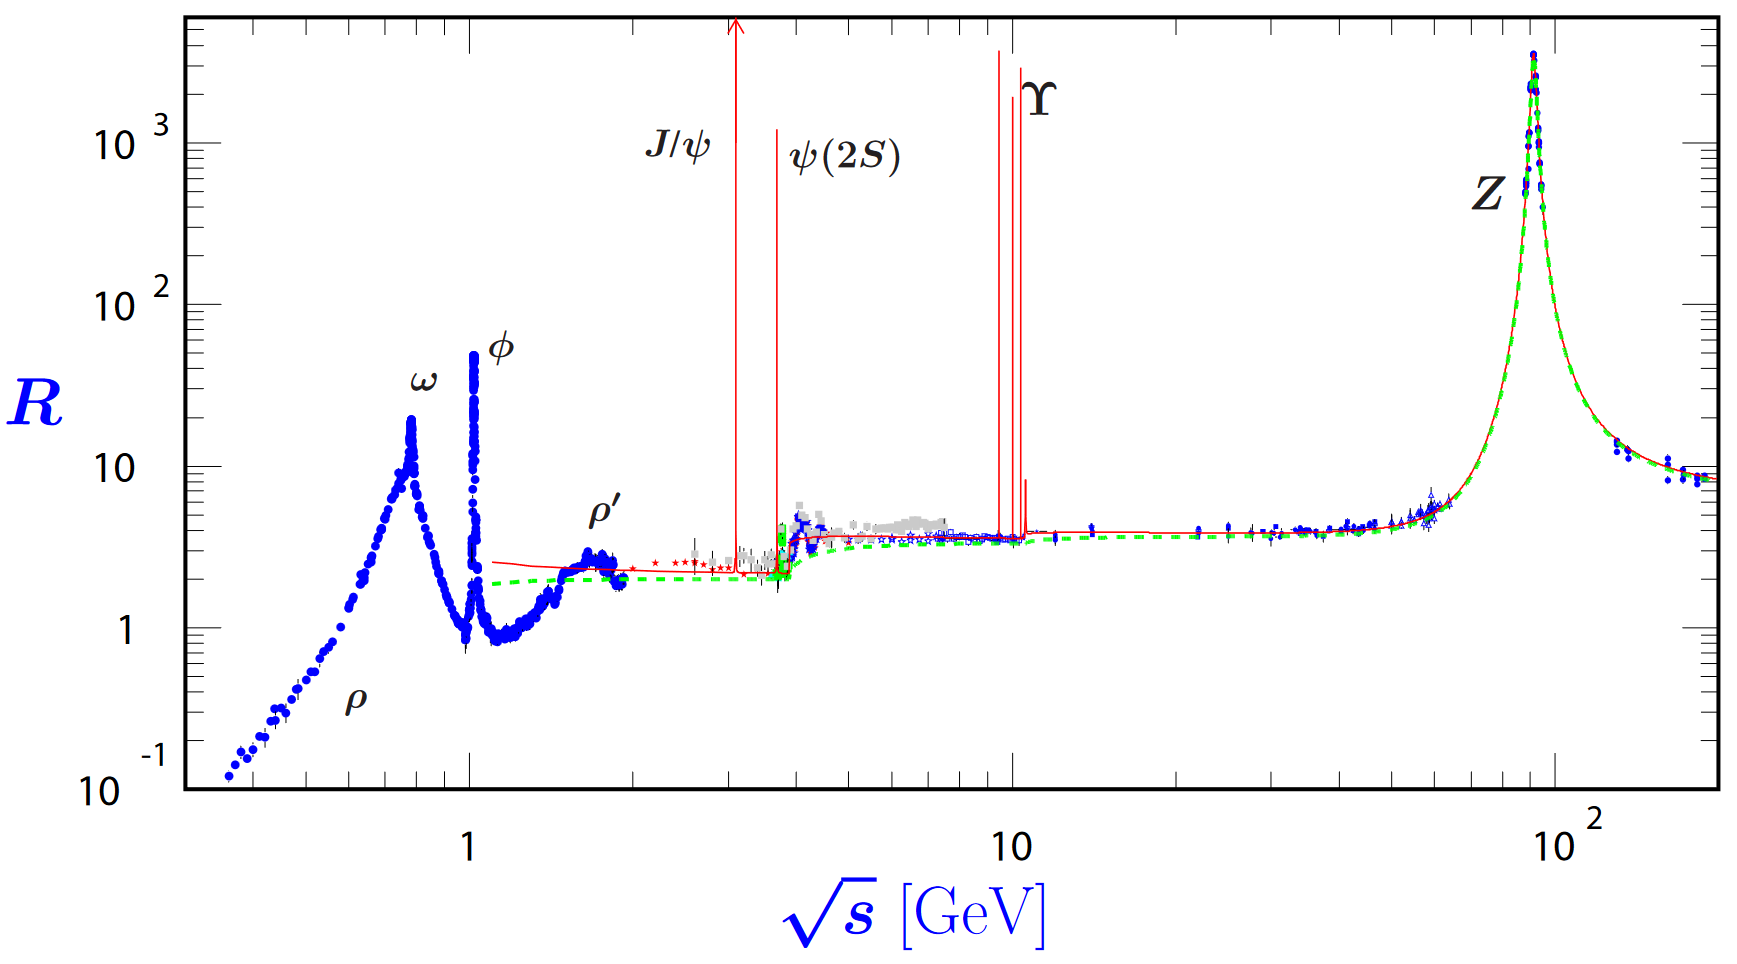
\includegraphics[width=0.8\textwidth]{images/hadron-muon-branching-ratio}
        \caption{Plot of both experimental and theoretical values of \(R\). The dashed green line is the result we have calculated using the naive quark model, but with the transition regions where new quarks become available treated correctly. The red line is the result of three loop perturbative QCD calculations. The points are data from various experiments. Notice that the two theoretical results align better, ignoring the spikes, at higher energies when the QCD coupling constant is smaller. The spikes correspond to QCD resonances, unstable bound states of quarks. The peak at the end occurs at the mass of the \PZ{} boson, where production of a nearly on-shell \PZ{} boson in place of the photon increases the amplitude.}
        \label{fig:electron positron to hadron vs muon}
    \end{figure}
    
    \chapter{Parton Model}
    \section{Low Energies}
    We want to discuss electron-proton scattering.
    How we think about the proton depends on the energy scale of the interaction.
    At low energies, \(q^2 \ll \Lambda_{\symrm{QCD}}\), we can treat the proton as a point particle, and consider QED scattering, which at tree level is
    \begin{equation}
        \tikzsetnextfilename{partons-point-like-scattering}
        \begin{tikzpicture}[baseline=(current bounding box)]
            \draw[electron] (-1, 1) node [left] {\(\Pe\)} -- (0, 0.5);
            \draw[electron] (0, 0.5) -- (1, 1) node [right] {\(\Pe\)};
            \draw[electron] (-1, -1) node [left] {\(\Pp\)} -- (0, -0.5);
            \draw[electron] (0, -0.5) -- (1, -1) node [right] {\(\Pp\)};
            \draw[photon] (0, 0.5) -- (0, -0.5);
            \draw[->] (0.2, 0.3) -- (0.2, -0.3) node [midway, right] {\(q\)};
        \end{tikzpicture}
        .
    \end{equation}
    This scattering is elastic, the particles before and after the interaction are the same, and so the kinetic energy is the same, although how its shared between the particles may change.
    Intuitively this is an appropriate description when the wavelength of the photon is much larger than the size of the proton.
    
    \section{Medium Energies}
    At intermediate energies, \(q^2 \sim \Lambda_{\symrm{QCD}}\), we have to consider the proton as a composite particle and the interaction looks more like
    \begin{equation}
        \tikzsetnextfilename{partons-medium-energy-scattering}
        \begin{tikzpicture}[baseline=(current bounding box)]
            \draw[electron] (-1, 1) node [left] {\(\Pe\)} -- (0, 0.5);
            \draw[electron] (0, 0.5) -- (1, 1) node [right] {\(\Pe\)};
            \coordinate (right) at (1, -1);
            \begin{scope}[yshift=-0.7cm]
                \draw[blob] (0, 0) circle [radius=0.2];
                \draw[electron] (206.565:1) node [left] {\(\Pp\)} -- (206.565:0.2);
                \draw (30:0.2) -- (0, 0.3 -| right);
                \draw (0.2, 0) -- (0, 0 -| right);
                \draw (-30:0.2) -- (0, -0.3 -| right);
                \draw[thick, decoration={calligraphic brace, mirror}, decorate] (1.1, -0.35) -- (1.1, 0.35) node [pos=0.55, right] {hadrons};
            \end{scope}
            \draw[photon] (0, 0.5) -- (0, -0.5);
            \draw[->] (0.2, 0.3) -- (0.2, -0.3) node [midway, right] {\(q\)};
        \end{tikzpicture}
        .
    \end{equation}
    In this regime the interactions are non-perturbative.
    Hadrons are being created in a complicated process.
    This makes the process inelastic.
    It is generally hard to work in this regime and there are very few theoretical tools for these sorts of computations.
    
    \section{Deep Inelastic Scattering}
    At high energies, \(q \gg \Lambda_{\symrm{QCD}}\), lots of particles are created and annihilate in the proton, we call these \define{partons}\index{parton}.
    The proton looks a bit like
    \begin{equation}
        \tikzsetnextfilename{partons-high-energy-proton}
        \begin{tikzpicture}[baseline=(current bounding box)]
            \fill[highlight!10] (0, 0) circle [radius = 2cm];
            \fill[highlight!90] (90:1) circle [radius=0.1];
            \fill[highlight!90] (210:1) circle [radius=0.1];
            \fill[highlight!90] (330:1) circle [radius=0.1];
            \draw[gluon] ($(90:1) + (-70:0.1)$) to[out=-70, in=130] ($(330:1) + (130:0.1)$);
            \draw[gluon] ($(210:1) + (50:0.1)$) to[out=50, in=-110] ($(90:1) + (-110:0.1)$);
            \draw[gluon] ($(330:1) + (170:0.1)$) to[out=170, in=10] ($(210:1) + (10:0.1)$);
            \draw[gluon] ($(90:1) + (0:0.1)$) to[out=0, in=70, bend left=70] ($(330:1) + (70:0.1)$);
            \draw[gluon] (-0.2, -1.2) to[bend left] ($(210:1) + (-90:0.1)$);
            \draw[dotted] (-0.2, -1.2) arc (180:0:0.2);
            \draw[dotted] (-0.2, -1.2) arc (180:360:0.2);
            \draw[gluon] (0.2, -1.2) to[in=90, bend right] ($(330:1) + (-90:0.1)$);
            \begin{scope}[rotate=-120]
                \draw[gluon] (-0.2, -1.2) to[bend left] ($(210:1) + (-90:0.1)$);
                \draw (-0.2, -1.2) arc (180:0:0.2);
                \draw (-0.2, -1.2) arc (180:360:0.2);
                \draw[gluon] (0.2, -1.2) to[in=90, bend right] ($(330:1) + (-90:0.1)$);
            \end{scope}
        \end{tikzpicture}
    \end{equation}
    where the three dots are the \enquote{valence} quarks, the ones that we think of as making up the proton, and the other particles are virtual.
    Intuitively, this regime is important when the wavelength of the photon is much less than the size of the proton.
    We call this \defineindex{deep inelastic scattering} (DIS)\glossary[acronym]{DIS}{Deep Inelastic Scattering}, the deep referring to the energies allowing us to probe \enquote{deep} into the proton.
    
    The problem is that while the interaction may occur at high enough energies for perturbation theory the initial state, the proton, is still non-perturbative.
    The solution is to use some physical reasoning.
    The momentum of the partons in the rest frame of the proton will be relatively low.
    This means that for sufficiently high momentum protons the momentum of the partons mostly aligns with the momentum of the proton.
    Hence the momentum of a parton can be expressed as
    \begin{equation}
        p^\mu = xP^\mu
    \end{equation}
    where \(P^\mu\) is the momentum of the proton and \(x\)\index{x@\(x\)|see{momentum fraction}} is the \defineindex{momentum fraction} of the parton, the fraction of the momentum that single parton carries.
    Since the momentum is carried entirely by the partons we must have
    \begin{equation}
        P^\mu = \sum_i p_i^\mu = \sum_i x_iP^\mu = P_\mu \sum_i x_i \implies \sum_i x_i = 1
    \end{equation}
    where \(p_i\) is the momentum carried by parton \(i\), which has momentum fraction \(x_i\).
    Strictly the partons momentum is only mostly aligned with the protons momentum, so actually we find that
    \begin{equation}
        \sum_i x_i = 1 + \order(\Lambda_{\symrm{QCD}}),
    \end{equation}
    since the momentum of the partons in the rest frame of the proton is on the order of \(\Lambda_{\symrm{QCD}}\).
    
    In order to utilise these momentum fractions we introduce the \define{parton distribution functions}\index{parton distribution function} (PDF)\glossary[acronym]{PDF}{Parton Distribution Function}, \(f_i\), which is defined such that \(f_i(x_i)\) is the probability density for finding parton \(i\) with momentum fraction \(x_i\).
    
    The other tool that we have is asymptotic freedom.
    This suggests that we can understand electron proton scattering at high energies as the interaction of a single parton with the electron.
    This looks a bit like
    \begin{equation}
        \tikzsetnextfilename{partons-deep-inelastic-scattering}
        \begin{tikzpicture}[font=\scriptsize, baseline=(current bounding box)]
            \draw[electron] (-1, 1) node [left] {\(\Pe\)} -- (0, 0.5);
            \draw[electron] (0, 0.5) -- (1, 1) node [right] {\(\Pe\)};
            \draw[electron] (-1, -1) -- (0, -0.5);
            \draw[electron] (0, -0.5) -- (1, -1) node [midway, below] {\(\Pq_i\)} coordinate (right);
            \begin{scope}[yshift=-0.5cm, shift={(206.656:1.318)}]
                \draw[blob] (0, 0) circle [radius=0.2];
                \draw (-1, 0) -- (-0.2, 0);
                \draw (200:1) -- (200:0.2);
                \draw (220:1) -- (220:0.2);
                \draw (0.2, 0) -- (0, -0.1 -| right);
                \draw (-30:0.2) -- (0, -0.3 -| right);
            \end{scope}
            \draw[photon] (0, 0.5) -- (0, -0.5);
            \draw[->] (0.2, 0.3) -- (0.2, -0.3) node [midway, right] {\(q\)};
            \draw[->] (-1.9, -1.85) -- (-1, -1.4) node [midway, below] {\(P\)};
            \draw[->, shift={(-0.1, 0.1)}, yshift=-0.5cm] (206.565:0.8) -- (206.565:0.2) node [midway, above, shift={(-0.3, -0.1)}] {\(p = xP\)};
            \draw[thick, decoration={calligraphic brace, mirror}, decorate, yshift=-1.2cm] (1.1, -0.3) -- (1.1, 0.3) node [pos=0.55, right] {hadrons};
        \end{tikzpicture}
        .
    \end{equation}
    
    We can define \(\sigma\) to be the total cross section for this interaction, and then the \defineindex{parton level cross section}, \(\hat{\sigma}_i\), to be the cross section for the interaction
    \begin{equation}
        \tikzsetnextfilename{partons-parton-level-scattering}
        \begin{tikzpicture}[baseline=(current bounding box)]
            \draw[electron] (-1, 1) node [left] {\(\Pe\)} -- (0, 0.5);
            \draw[electron] (0, 0.5) -- (1, 1) node [right] {\(\Pe\)};
            \draw[electron] (-1, -1) node [left] {\(\Pp_i\)} -- (0, -0.5);
            \draw[electron] (0, -0.5) -- (1, -1) node [right] {\(\Pp_i\)};
            \draw[photon] (0, 0.5) -- (0, -0.5);
            \draw[->] (0.2, 0.3) -- (0.2, -0.3) node [midway, right] {\(q\)};
        \end{tikzpicture}
    \end{equation}
    The total cross section is simply given by summing over all possible partons which could take part in the interaction, and integrating over all possible momentum fractions that they can have, including the parton distribution function, \(f_i\), for each parton to properly account for the probability of it having a given share of the momentum.
    That is,
    \begin{equation}
        \sigma = \sum_i \int_0^1 \dl{x} \, f_i(x) \hat{\sigma}_i(x).
    \end{equation}
    This is the \defineindex{factorisation formula}.
    It splits the physics into two parts:
    \begin{itemize}
        \item The parton distribution function contains the non-perturbative physics associated with the initial state, the proton.
        This is a low energy quantity.
        We can measure the PDF once and then it will be the same for all processes, it is, in this sense, universal.
        It does depend on the type of particle, so the PDF will be different for a pion or a \(\PDeltapp\).
        \item The parton level cross section contains all of the perturbative physics.
        It is calculated in perturbative QCD and QED.
        It is a high energy quantity, so we can use asymptotic freedom.
        It is specific to a given process.
    \end{itemize}
    
    Feynman originally introduced the parton model, and the factorisation formula, following much the same logic as we have here, but impressively did it before quarks and gluons were understood to be the (majority of) partons.
    Perhaps surprisingly this formula treats the scattering of partons as being incoherent, we don't add the amplitudes and the square to get the cross section, instead we find the individual parton level cross sections and simply add these.
    This is justified because scattering occurs on a very short time scale, so we can essentially ignore the particles not directly involved in the scattering and there is no interference.
    
    We can extend the hat notation and parton level quantities to define
    \begin{equation}
        s = (P + k)^2, \qqand \hat{s} = (p + k)^2 = (xP + k)^2
    \end{equation}
    as the hadron and parton level \(s\) Mandelstam variable respectively, where \(k\) is the momentum of the incoming electron.
    This extends to other variables, such as \(\hat{t}\) and \(\hat{u}\) in the obvious way:
    \begin{equation}
        \hat{t} = (k - k')^2 = q^2, \qqand \hat{u} = (k' - p)^2 = (k' - xP)^2
    \end{equation}
    where \(k'\) is the momentum of the outgoing electron.
    
    \section{Drell--Yan Process}
    The \defineindex{Drell--Yan process} is scattering of two protons into leptons and hadrons, \(\Pp\Pp \to \ell^+\ell^- + \Phadrons\).
    We can picture this as
    \begin{equation}
        \tikzsetnextfilename{partons-drell-yan}
        \begin{tikzpicture}[font=\scriptsize, baseline=(current bounding box)]
            \draw[blob] (0, 0) circle [radius=0.2];
            \draw (140:0.2) -- (160:1);
            \draw (220:0.2) -- (200:1);
            \draw (180:0.2) -- (180:1);
            \draw[electron=0.6] (0:0.2) -- (30:1) coordinate (i) node [midway, left] {\(\Pq_i\)};
            \draw[->, shift={(0.15, -0.15)}] (25:0.3) -- (30:0.7) node [midway, below right, shift={(-0.15, 0.1)}] {\(p_1 = x_1P_1\)};
            \begin{scope}[yshift=1cm]
                \draw[blob] (0, 0) circle [radius=0.2];
                \draw (140:0.2) -- (160:1);
                \draw (220:0.2) -- (200:1);
                \draw (180:0.2) -- (180:1);
                \draw[positron=0.4] (0:0.2) -- (-30:1) node [midway, left] {\(\APq_i\)};
                \draw[->, shift={(0.15, 0.15)}] (-25:0.3) -- (-30:0.7) node [midway, above right, shift={(-0.15, -0.05)}] {\(p_2 = x_2P_2\)};
            \end{scope}
            \draw[photon] (i) -- ++ (1, 0) coordinate (i2);
            \draw[electron=0.6] (i2) -- ++ (45:1) node [right] {\(\ell^-\)};
            \draw[positron=0.4] (i2) -- ++ (-45:1) node [right] {\(\ell^+\)};
            \draw[->] (-0.2, -0.3) -- (0.2, -0.3) node [midway, below] {\(P_1\)};
            \draw[->] (-0.2, 1.3) -- (0.2, 1.3) node [midway, above] {\(P_2\)};
        \end{tikzpicture}
        .
    \end{equation}
    
    This process involves two hadrons, so we have two momentum fractions, and two parton distribution functions, other than that the result is exactly  the same:
    \begin{equation}
        \sigma = \sum_{i, \overbar{\imath}} \int_0^1 \dl{x_1} \int_0^1 \dl{x_2} \, f_i(x_1)f_{\overbar{\imath}}(x_2) \hat{\sigma}_{i\overbar{\imath}}
    \end{equation}
    where \(i\) is summed over particles and \(\overbar{\imath}\) over antiparticles, and \(\hat{\sigma}_{i\overbar{\imath}}\) is the parton level cross section for the process \(\Pq_i\APq_i \to \ell^-\ell^+\).
    
    \chapter{Deep Inelastic Scattering}
    \section{The Process}
    Consider the process \(\Pp \Pe \to \Pe + \Phadrons\):
    \begin{equation}
        \tikzsetnextfilename{DIS-deep-inelastic-scattering}
        \begin{tikzpicture}[font=\scriptsize, baseline=(current bounding box)]
            \draw[electron] (-1, 1) node [left] {\(\Pe\)} -- (0, 0.5);
            \draw[electron] (0, 0.5) -- (1, 1) node [right] {\(\Pe\)};
            \draw[electron] (-1, -1) -- (0, -0.5);
            \draw[electron] (0, -0.5) -- (1, -1) node [midway, below] {\(\Pq_i\)} coordinate (right);
            \begin{scope}[yshift=-0.5cm, shift={(206.656:1.318)}]
                \draw[blob] (0, 0) circle [radius=0.2];
                \draw (-1, 0) -- (-0.2, 0);
                \draw (200:1) -- (200:0.2);
                \draw (220:1) -- (220:0.2);
                \draw (0.2, 0) -- (0, -0.1 -| right);
                \draw (-30:0.2) -- (0, -0.3 -| right);
            \end{scope}
            \draw[photon] (0, 0.5) -- (0, -0.5);
            \draw[->] (0.2, 0.3) -- (0.2, -0.3) node [midway, right] {\(q = k - k'\)};
            \draw[->] (-1.9, -1.85) -- (-1, -1.4) node [midway, below] {\(P\)};
            \draw[->, shift={(-0.1, 0.1)}, yshift=-0.5cm] (206.565:0.8) -- (206.565:0.2) node [midway, above, shift={(-0.3, -0.1)}] {\(p = xP\)};
            \draw[thick, decoration={calligraphic brace, mirror}, decorate, yshift=-1.2cm] (1.1, -0.3) -- (1.1, 0.3) node [pos=0.55, right] {hadrons};
            \draw[->, shift={(-0.9, 1.1)}] (-26.565:0.2) -- (-26.565:0.8) node [midway, above right, shift={(-0.1, -0.1)}] {\(k\)};
            \draw[->, shift={(-0.05, 0.61)}] (26.565:0.2) -- (26.565:0.8) node [midway, above left, shift={(0.15, -0.1)}] {\(k'\)};
            \draw[->, shift={(0.1, -0.4)}] (-26.565:0.2) -- (-26.565:0.8) node [midway, above right, shift={(-0.1, -0.1)}] {\(p'\)};
        \end{tikzpicture}
        .
    \end{equation}
    
    We can calculate the parton level cross section for this process, it's just a QED interaction between the electron and a quark.
    The problem comes when we try to compute the total cross section.
    Ideally we would do the kinematics in the parton centre of mass frame, since this makes things a lot simpler when we also neglect the electron mass.
    However, we don't know what the parton centre of mass frame is, since we don't know the momentum of the parton.
    
    We will assume that the masses of the particles involved in this interaction are negligible, but also that we are at low enough energies that we don't have to worry about \PZ{} bosons as exchange particles.
    We can easily compute the parton level amplitude, and then the amplitude squared, averaged over initial states and summed over final states.
    The result is
    \begin{equation}
        \frac{1}{4}\sum_{\text{spins}} \abs{\amplitude_i}^2 = 2Q_i^2 e^4 \frac{\hat{s}^2 + \hat{u}^2}{\hat{t}^2}.
    \end{equation}
    This is just the \(t\)-channel electron positron or electron muon scattering process, but with an extra factor of \(Q_i\) in the amplitude and using parton level values, \(\hat{t} = q^2\), \(\hat{s} = (k + p)^2 = (k + xP)^2\), and \(\hat{u} = (k' - p)^2 = (k' - xP)^2\).
    
    In the parton centre of mass frame the cross section is, as usual, given by
    \begin{equation}
        \diff{\hat{\sigma}_i}{\Omega} = \frac{1}{64\pi^2\hat{s}} \frac{1}{4}\sum_{\text{spins}} \abs{\amplitude_i} = \frac{1}{64\pi^2\hat{s}} 2Q_i^2 e^4 \frac{\hat{s}^2 + \hat{u}^2}{\hat{t}^2}.
    \end{equation}
    This can be rewritten as
    \begin{equation}
        \diff{\hat{\sigma}_i}{(\cos\vartheta)} = \frac{1}{32\pi\hat{s}}2Q_i^2 e^4\frac{\hat{s}^2 + \hat{u}^2}{\hat{t}^2}.
    \end{equation}
    
    \section{Experimentally Accessible Variables}
    We'll first consider \(\hat{t}\).
    As the square of a four-vector this is a Lorentz invariant, so we can calculate it in any frame.
    Choose the frame where the initial electron is moving along the \(x\)-axis.
    Further, neglecting the electron mass we have \(k^2 = 0\), and so we can write \(k^\mu = (E, E, 0, 0)\).
    The momentum of the outgoing electron is then \(k'^\mu = (E, E\vh{n})\), where \(\vh{n}\) is a unit three-vector.
    In this frame we have
    \begin{equation}
        \hat{t} = (k - k')^2 = -2k\cdot k' = -2E^2(1 - \cos\vartheta) = -\frac{\hat{s}^2}{2}(1 - \cos\vartheta),
    \end{equation}
    where we've used \(\hat{s} = (2E)^2\), this is just the usual result that the \(s\) Mandelstam invariant gives the energy coming into the process squared, assuming both the parton and electron have the same energy, which is usually true in scattering experiments.
    
    For the differential cross section we can use \(\hat{t}\) as the differential quantity, using
    \begin{equation}
        \dl{\hat{t}} = \frac{\hat{s}}{2} \dd{(\cos\vartheta)}.
    \end{equation}
    Here we've used the fact that the three Mandelstam invariants are pairwise independent, so differentials in \(\dl{\hat{t}}\) don't need to change \(\hat{s}\).
    Using this we have
    \begin{equation}
        \diff{}{(\cos\vartheta)} = \frac{\hat{s}}{2}\diff{}{\hat{t}}.
    \end{equation}
    This allows us to write
    \begin{equation}
        \diff{\hat{\sigma}_i}{\hat{t}} = \frac{2}{\hat{s}} \diff{\hat{\sigma}_i}{(\cos\vartheta)} = 2\pi \alpha^2 Q_i^2 \frac{\hat{s}^2 + (\hat{t} + \hat{s})^2}{\hat{s}^2 \hat{t}^2} = 2\pi \alpha^2 Q_i^2 \frac{1 + (1 + \hat{t}/\hat{s})^2}{\hat{t}^2}.
    \end{equation}
    Here we've used \(\hat{u} = -\hat{t} - \hat{s}\) to replace the \(\hat{u}\) Mandelstam invariant with \(\hat{s}\) and \(\hat{t}\) which we have a better handle on.
    
    There is a problem with this result though.
    While we may know the energy of the electron and proton we don't know what share of this energy any given parton has.
    The quantities which are experimentally accessible are
    \begin{itemize}
        \item Anything to do with the electron, including its momenta, \(k\) and \(k'\), and the Mandelstam invariant \(\hat{t} = (k - k')^2\).
        \item Anything to do with the incoming proton, such as its momentum, \(P\), and the proton level Mandelstam invariant \(s = (k + P)^2 \approx 2k \cdot P\).
    \end{itemize}
    Parton level data is generally inaccessible unless it is related to the above data through, for example, momentum conservation.
    For example, the parton level Mandelstam invariant \(\hat{s}\) is actually accessible since \(\hat{s} = (k + p)^2 = 2k\cdot p = 2xk \cdot P\) and it turns out that, somewhat surprisingly, \(x\) is actually observable under the assumption that the incoming and outgoing partons are on-shell.
    This is a safe assumption if the partons travel for a long time relative to the interaction time, or equivalently if the interaction energy is high compared to \(\Lambda_{\symrm{QCD}}\).
    This is the case generally, for example in the LHC where \(\sqrt{s} = \qty{13.6}{\tera\electronvolt}\).
    This means that the interaction time goes as
    \begin{equation}
        \hbar/(\qty{13.6}{\tera\electronvolt}) \ll \hbar/\Lambda_{\symrm{QCD}} \sim 10^{-23}\,\unit{\second}.
    \end{equation}
    Corrections for the partons not really being on-shell then are suppressed by factors of \(\Lambda_{\symrm{QCD}}^2/q^2\).
    
    Assuming that the parton mass is also negligible, so \(p'^2 \approx 0\), we have \((p + q)^2 \approx 2p \cdot q + q^2\).
    Thus, in terms of the proton momentum we have \(2x P \cdot q = -q^2\).
    Rearranging this gives us the \defineindex{Bjorken formula}
    \begin{equation}
        x = \frac{-q^2}{2P \cdot q} = \frac{\hat{t}}{2P \cdot q}.
    \end{equation}
    The right hand side consists of experimentally measurable quantities.
    The quantity \(x\) is sometimes called the \define{Bjorken \(\bm{x}\)}\index{Bjorken x@Bjorken \(x\)}.
    
    Notice that \(\hat{t} \le 0\) since
    \begin{equation}
        \hat{t} = -\frac{\hat{s}}{2}(1 - \cos\vartheta)
    \end{equation}
    and \(\abs{\cos\vartheta} \le 1\) and \(\hat{s} = (2E)^2 \ge 0\).
    We therefore define a positive measure of energy transfer, \(Q^2 \coloneqq -\hat{t}\).
    Then
    \begin{equation}
        x = \frac{Q^2}{2P\cdot q}.
    \end{equation}
    In terms of this quantity we have
    \begin{equation}
        \diff{\hat{\sigma}_i}{Q^2} = -\diff{\hat{\sigma}_i}{\hat{t}} = 2\pi\alpha^2 Q_i^2 \frac{1 + (1 - Q^2/(xs))^2}{Q^4}.
    \end{equation}
    
    Both \(\hat{t}\) and \(x\) are experimentally accessible, so we can make use of a doubly differential cross section at the hadron level:
    \begin{equation}
        \diff{\sigma}{x,Q^2} = \sum_i f_i(x) 2\pi \alpha^2 Q_i^2 \frac{1 + (1 - Q^2/(xs))^2}{Q^4}.
    \end{equation}
    Hence the total cross section is
    \begin{equation}
        \sigma = \int_0^1 \dl{x} \int \dl{Q^2} \diff{\sigma}{x,Q^2}.
    \end{equation}
    
    It is possible to give a more general form for the differential cross section:
    \begin{equation}
        \diff{\sigma}{x,Q^2} = \frac{2\pi\alpha^2}{xQ^4} \left[ \left( 1 + \left[ 1 - \frac{Q^2}{xs} \right]^2 \right) F_2(x, Q^2) - \left( \frac{Q^2}{xs} \right) F_{L}(x, Q^2) \right],
    \end{equation}
    The two functions \(F_2\) and \(F_L\) parametrise a more general interaction, we've considered a QED interaction here, but there could also be weak interactions.
    Our result is just the special case where
    \begin{equation}
        F_2(x, Q^2) = \sum_i x f_i(x), \qqand F_L(x, Q^2) = 0.
    \end{equation}
    It turns out that \(F_L\) vanishes for fermionic partons.
    This is evidence that quarks have spin \(1/2\), which we need since we can't see quarks on their own.
    
    \part{Infrared Divergences}
    \chapter{Infrared Divergences}
    \textit{This new material in this part of the course is not examinable.}
    
    We have now spent a great deal of time studying divergences as momenta go to infinity.
    These are called \enquote{ultraviolet divergences}.
    It turns out that since lots of quantities go as one over momentum to some power we also get divergences when momenta go to zero.
    These are called \defineindex{infrared divergences}.
    In this part of the course we will look at how to deal with these divergences.
    Infrared divergences occur in most quantum field theories, so for simplicity we will mostly focus on QED, although we'll start with QCD as the motivation.
    
    
    
    %%%%%%%%%%%%%%%%%%%%%%%%%%%%%%%%%%%%%%%%%%%%%%%%%%%%%%%%%%%%%%%%%%%%%%%%%%%%%%%%%%%%%%%%%%%%%%%%%%%%%%%%%%%%%%
    
    
    
    
    
    
    \renewcommand{\amplitude}{\symcal{M}}    
    
    
    
    
    
    
    
    
    
    
    
    
    
    
    %%%%%%%%%%%%%%%%%%%%%%%%%%%%%%%%%%%%%%%%%%%%%%%%%%%%%%%%%%%%%%%%%%%%%%%%%%%%%%%%%%%%%%%%%%%%%%%%%%%%%%%%%%%%%%
    
    \part{Electroweak}
    \chapter{Overview}
    There are four fundamental forces,
    \begin{itemize}
        \item electromagnetism;
        \item the strong force;
        \item the weak force;
        \item gravity.
    \end{itemize}
    In this course we are interested in the first three.
    To each force we can associate a type of radiation,
    \begin{itemize}
        \item gamma radiation;
        \item alpha radiation;
        \item beta radiation;
        \item gravitational waves.
    \end{itemize}
    These forces all have different ranges, reflecting the different mechanisms behind the difference forces, at long ranges these forces scale as
    \begin{itemize}
        \item \(1/r\);
        \item \(\e^{-\mu r}/r\) with \(\mu \approx \qty{1}{\giga\electronvolt}\);
        \item \(\e^{-\mu r}\) with \(\mu \approx \qty{100}{\giga\electronvolt}\);
        \item \(1/r\).
    \end{itemize}
    Each of these forces can be described as a gauge theory with a different gauge group,
    \begin{itemize}
        \item \(\unitary(1)\);
        \item \(\specialUnitary(3)\);
        \item \(\specialUnitary(2)\);
        \item diffeomorphisms of spacetime\footnote{some don't consider this to be a gauge theory, for one thing the group of diffeomorphisms is non-compact, and the theory doesn't work in quite the same way as the other examples.}.
    \end{itemize}
    No one is quite sure why these particular gauge groups are the ones which apply in each case, and the choice of gauge group pretty much completely determines the physics.
    For example, the fact that \(\specialUnitary(3)\) and \(\specialUnitary(2)\) are non-Abelian is responsible for the short range interactions of the strong and weak force, which is ultimately due to the self interactions of exchange particles, which doesn't occur in the Abelian \(\unitary(1)\) case.
    
    One of the main tools in our arsenal is perturbation theory, although this doesn't work in all cases
    \begin{itemize}
        \item perturbation theory works at sufficiently low energies, including most cases of real world interest;
        \item perturbation theory works at high energies, but not low energies;
        \item perturbation theory works but is \enquote{weird} and \enquote{interesting};
        \item perturbation theory works for sufficiently small perturbations.
    \end{itemize}
    
    Symmetry is important in physics, these forces posses, or don't posses, various symmetries.
    One symmetry being preserving flavour, that is the type of fermion involved in interactions,
    \begin{itemize}
        \item flavour stays the same;
        \item flavour stays the same;
        \item flavours can change;
        \item flavours stay the same.
    \end{itemize}
    Another set of symmetries is parity (\(\parity\)), charge conjugation (\(\chargeConjugation\)), and time reversal (\(\timeReversal\)), although often due to the \(\chargeConjugation\parity\timeReversal\) theorem, which states that the combination of all three of these symmetries is respected, we replace time reversal, which is weird involving anti-unitary operations, with charge conjugation and parity transformation (\(\chargeConjugation\parity\)).
    \begin{itemize}
        \item \(\parity\), \(\chargeConjugation\), and \(\timeReversal\) are all respected;
        \item \(\parity\), \(\chargeConjugation\), and \(\timeReversal\) are all respected;
        \item \(\parity\) and \(\chargeConjugation\) are maximally violated, \(\chargeConjugation\parity\) is violated a very small amount;
        \item GR respects these symmetries, other theories of gravity do not.
    \end{itemize}
    
    Each force allows for different interactions,
    \begin{itemize}
        \item
        \tikzsetnextfilename{overview-vertex-qed}
        \begin{tikzpicture}[baseline=(base.base)]
            \draw[electron] (-1, 0) node [left] (base) {\(\Pe\)}-- (0, 0);
            \draw[electron] (0, 0) -- (1, 0) node [right] {\(\Pe\)};
            \draw[photon] (0, 0) -- (0, 1) node [above] {\(\Pphoton\)};
        \end{tikzpicture}
        \kern-0.6em, and the same with \(\Pmu\) and \(\Ptau\)
        \item
        \tikzsetnextfilename{overview-vertex-qcd-qqg}
        \begin{tikzpicture}[baseline=(base.base)]
            \draw[quark] (-1, 0) node [left] {\(\Pq\)} -- (0, 0);
            \draw[quark] (0, 0) -- (1, 0) node [right] (base) {\(\Pq\)};
            \draw[gluon] (0, 0) -- (0, 1) node [above] {\(\Pg\)};
        \end{tikzpicture}
        \kern-0.6em,
        \tikzsetnextfilename{overview-vertex-qcd-ggg}
        \begin{tikzpicture}[baseline=(base.base)]
            \draw[gluon] (0, 0) -- (210:0.7) node [left] {\(\Pg\)};
            \draw[gluon] (0, 0) -- (330:0.7) node [right] (base) {\(\Pg\)};
            \draw[gluon] (0, 0) -- (90:0.7) node [above] {\(\Pg\)};
        \end{tikzpicture}
        \kern-0.6em,
        \tikzsetnextfilename{overview-vertex-qcd-gggg}
        \begin{tikzpicture}[baseline=(base.base)]
            \draw[gluon] (0, 0) -- (45:0.7) node [right] {\(\Pg\)};
            \draw[gluon] (0, 0) -- (135:0.7) node [left] {\(\Pg\)};
            \draw[gluon] (0, 0) -- (225:0.7) node [left] (base) {\(\Pg\)};
            \draw[gluon] (0, 0) -- (315:0.7) node [right] {\(\Pg\)};
        \end{tikzpicture}
        \item \begingroup\raggedright
        \tikzsetnextfilename{overview-vertex-ew-enuw}
        \begin{tikzpicture}[baseline=(base.base)]
            \draw[electron] (-1, 0) node [left] {\(\PeLeft\)}-- (0, 0);
            \draw[electron] (0, 0) -- (1, 0) node [right] (base) {\(\PnueLeft\)};
            \draw[WZ boson] (0, 0) -- (0, 1) node [above] {\(\PW\)};
        \end{tikzpicture}
        \kern-0.55em, and the same with \(\PmuLeft\) and \(\PnumuLeft\), and \(\PtauLeft\) and \(\PnutauLeft\),\\
        \tikzsetnextfilename{overview-vertex-ew-eez}
        { % don't line break before the comma
        \begin{tikzpicture}[baseline=(base.base)]
            \draw[electron] (-1, 0) node [left] (base) {\(\Pe\)}-- (0, 0);
            \draw[electron] (0, 0) -- (1, 0) node [right] {\(\Pe\)};
            \draw[photon] (0, 0) -- (0, 1) node [above] {\(\PZ\)};
        \end{tikzpicture}
        \kern-0.6em,} and the same with \(\Pmu\) and \(\Ptau\),\\
        { % don't line break before the comma
        \tikzsetnextfilename{overview-vertex-ew-udw}
        \begin{tikzpicture}[baseline=(base.base)]
            \draw[quark] (-1, 0) node [left] {\(\Pu_{\Left}\)}-- (0, 0);
            \draw[quark] (0, 0) -- (1, 0) node [right] (base) {\(\Pd_{\Left}\)};
            \draw[WZ boson] (0, 0) -- (0, 1) node [above] {\(\PW\)};
        \end{tikzpicture}
        \kern-0.6em,} and the same with \(\Pc_{\Left}\) and \(\Ps_{\Left}\), and \(\Pt_{\Left}\) and \(\Pb_{\Left}\),\\
        \tikzsetnextfilename{overview-vertex-ew-qqz}
        \begin{tikzpicture}[baseline=(base.base)]
            \draw[electron] (-1, 0) node [left] (base) {\(\Pq\)}-- (0, 0);
            \draw[electron] (0, 0) -- (1, 0) node [right] {\(\Pq\)};
            \draw[photon] (0, 0) -- (0, 1) node [above] {\(\PZ\)};
        \end{tikzpicture}
        \kern-0.55em,
        \tikzsetnextfilename{overview-vertex-ew-www}
        \begin{tikzpicture}[baseline=-0.31cm]
            \draw[WZ boson] (0, 0) -- (210:0.7);
            \draw[WZ boson] (0, 0) -- (330:0.7);
            \draw[WZ boson] (0, 0) -- (90:0.7);
        \end{tikzpicture}
        and
        \tikzsetnextfilename{overview-vertex-wwww}
        \begin{tikzpicture}[baseline=-0.5cm]
            \draw[WZ boson] (0, 0) -- (45:0.7);
            \draw[WZ boson] (0, 0) -- (135:0.7);
            \draw[WZ boson] (0, 0) -- (225:0.7);
            \draw[WZ boson] (0, 0) -- (315:0.7);
        \end{tikzpicture}
        with the particles being any of \(\PW\), \(\PZ\), or \(\Pphoton\), so long as charge is conserved, 
        \tikzsetnextfilename{overview-vertex-ew-ffh}
        \begin{tikzpicture}[baseline=(base.base)]
            \draw[electron] (-1, 0) node [left] (base) {\(\Pf\)}-- (0, 0);
            \draw[electron] (0, 0) -- (1, 0) node [right] {\(\Pf\)};
            \draw[higgs] (0, 0) -- (0, 1) node [above] {\(\Phiggs\)};
        \end{tikzpicture}
        \kern-0.5em,\\
        \tikzsetnextfilename{overview-vertex-ew-wwh}
        \begin{tikzpicture}[baseline=(base.base)]
            \draw[WZ boson] (-1, 0) node [left] (base) {\(\PW\)/\(\PZ\)}-- (0, 0);
            \draw[WZ boson] (0, 0) -- (1, 0) node [right] {\(\PW\)/\(\PZ\)};
            \draw[higgs] (0, 0) -- (0, 1) node [above] {\(\Phiggs\)};
        \end{tikzpicture}
        \kern-0.5em,
        \tikzsetnextfilename{overview-vertex-wwhh}
        { % don't line break before the comma
        \begin{tikzpicture}[baseline=(base.base)]
            \draw[higgs] (0, 0) -- (45:0.7) node [right] {\(\Phiggs\)};
            \draw[higgs] (0, 0) -- (135:0.7) node [left] {\(\Phiggs\)};
            \draw[WZ boson] (0, 0) -- (225:0.7) node [left] (base) {\(\PW\)/\(\PZ\)};
            \draw[WZ boson] (0, 0) -- (315:0.7) node [right] {\(\PW\)/\(\PZ\)};
        \end{tikzpicture}
        \kern-0.55em,}
        \tikzsetnextfilename{overview-vertex-hhh}
        \begin{tikzpicture}[baseline=(base.base)]
            \draw[higgs] (0, 0) -- (210:0.7) node [left] {\(\Phiggs\)};
            \draw[higgs] (0, 0) -- (330:0.7) node [right] (base) {\(\Phiggs\)};
            \draw[higgs] (0, 0) -- (90:0.7) node [above] {\(\Phiggs\)};
        \end{tikzpicture}
        \kern-0.6em,\\
        and
        \tikzsetnextfilename{overview-vertex-hhhh}
        \begin{tikzpicture}[baseline=(base.base)]
            \draw[higgs] (0, 0) -- (45:0.7) node [right] {\(\Phiggs\)};
            \draw[higgs] (0, 0) -- (135:0.7) node [left] {\(\Phiggs\)};
            \draw[higgs] (0, 0) -- (225:0.7) node [left] (base) {\(\Phiggs\)};
            \draw[higgs] (0, 0) -- (315:0.7) node [right] {\(\Phiggs\)};
        \end{tikzpicture}
        , note that interactions involving a photon or Higgs boson are due to the electroweak interaction, rather than just the weak interaction;
        \endgroup
        \item depends on your theory of gravity.
    \end{itemize}
    
    \section{The Weak Force}
    As we saw in the previous section the weak force is quite different from electromagnetism and the strong force, which really only differ due to \(\unitary(1)\) being Abelian and \(\specialUnitary(2)\) being non-Abelian.
    The weak force allows for flavour change, and includes many more interactions than either electromagnetism or the strong interaction.
    
    Examples of processes mediated by the weak force are \defineindex{beta decay},
    \begin{equation}
        \Pneutron \to \Pproton \Pe \APnue, \qquad \Pu\Pd\Pd \to \Pu\Pu\Pd \Pe \APnue,
    \end{equation}
    \define{pion decays}\index{pion decay}, such as
    \begin{equation}
        \Ppim \to \Pmu\APnumu, \qquad \Ppim \to \Pe\APnue, \qquad \Ppizero \to \Pphoton\Pphoton, \qquad \Ppizero \to \Pphoton \Pe \APe,
    \end{equation}
    and \define{kaon decays}\index{kaon decay}, such as
    \begin{equation}
        \PKm \to \Ppim \Ppizero, \qquad \PKm \to \Ppim \Ppim \Ppip.
    \end{equation}
    
    The violation of symmetries and the ability of the weak force to change the flavour of particles makes the world a much more interesting place.
    Without out this the universe would be static, up to uninteresting dynamical changes, with lepton and quark number remaining constant.
    The fact that the weak force allows for decays also means that if we reverse time, despite the symmetry breaking, the weak force allows for creation of particles as well, and this is one of the major avenues of study for early universe physics.
    
    In this course we will follow a historical approach, piecing together first the theory of the weak interaction, and then combining this with electromagnetism to get electroweak theory.
    As such there will be points where we study theories which later turned out to be wrong, or at least not the complete picture.
    
    The theory of weak interactions begins with Pauli in 1930 who was studying the kinematics of beta decay and realised that seemingly missing energy could be explained if the decay was producing another particle, the neutrino.
    The neutrino's existence was the confirmed experimentally in 1956 by Frederick Reines and Clyde Cowan\footnote{Nobel prize for (electro)weak theory count: 1}.
    In the time between positing the existence of the neutrino and its experimental confirmation the theory of the weak interaction had progressed a lot.
    In the same year Chien-Shiung Wu\footnote{Nobel prize for (electro)weak theory count: 2} observed parity violation for the first time, which was a big surprise, since the prevailing wisdom was that parity was always conserved.
    
    Before we can discus the weak force further we need to recap chirality, helicity, and parity.
    
    \chapter{Left and Right}
    \section{Chirality}
    Recall that the fifth gamma matrix is defined as
    \begin{equation}
        \gamma^5 = i\gamma^0 \gamma^1 \gamma^2 \gamma^3,
    \end{equation}
    and is such that \((\gamma^5)^2 = 1\), \((\gamma^5)^\hermit = \gamma^5\), and \(\anticommutator{\gamma^5}{\gamma^\mu} = 0\).
    Using this we can define a complete set of Hermitian, orthogonal projection operators:
    \begin{equation}
        P_{\Left} \coloneqq \frac{1}{2}(1 - \gamma^5), \qqand P_{\Right} \coloneqq \frac{1}{2}(1 + \gamma^5).
    \end{equation}
    We call these the left and right projection operators respectively, we'll justify this name later.
    Breaking it down \enquote{complete set of Hermitian, orthogonal projection operators} tells us the following:
    \begin{itemize}
        \item Projectors: \(P_{\Left}^2 = (1 - \gamma^5)^2/4 = (1 - 2\gamma^5 + 1)/4 = (1 - \gamma^5)/2 = P_{\Left}\), and similarly \(P_{\Right}^2 = P_{\Right}\);
        \item Orthogonal: \(P_{\Left}P_{\Right} = (1 - \gamma^5)(1 + \gamma^5)/2 = (1 - (\gamma^5)^2)/2 = (1 - 1)/2 = 0\), and similarly \(P_{\Right}P_{\Left} = 0\);
        \item Complete: \(P_{\Left} + P_{\Right} = (1 - \gamma^5)/2 + (1 + \gamma_5)/2 = 1\);
        \item Hermitian: \(P_{\Left}^\hermit = [(1 - \gamma^5)/2]^{\hermit} = (1 - (\gamma^5)^\hermit)/2 = (1 - \gamma^5)/2 = P_{\Left}\), and similarly \(P_{\Right}^\hermit = P_{\Right}\).
    \end{itemize}
    Note that we have \(P_{\Right} - P_{\Left} = (1 + \gamma^5)/2 - (1 - \gamma^5)/2 = \gamma^5\).
    Another useful property is that commuting a \(\gamma^\mu\) with a projector turns left into right and vice versa, so \(\gamma^\mu P_{\Left} = \gamma^\mu(1 - \gamma^5)/2 = (\gamma^\mu - \gamma^\mu \gamma^5)/2 = (\gamma^\mu + \gamma^5 \gamma^\mu)/2 = (1 + \gamma^5)\gamma^\mu/2 = P_{\Right}\gamma^\mu\), and similarly \(\gamma^\mu P_{\Right} = P_{\Left}\gamma^\mu\).
    
    Given a (Dirac) spinor, \(\psi\), we can decompose it into left and right components using
    \begin{equation}
        \psi = 1\psi = (P_{\Left} + P_{\Right})\psi = P_{\Left}\psi + P_{\Right}\psi = \psi_{\Left} + \psi_{\Right},
    \end{equation}
    where
    \begin{equation}
        \psi_{\Left} \coloneqq P_{\Left}\psi, \qqand \psi_{\Right} \coloneqq P_{\Right}\psi
    \end{equation}
    are the left and right components of \(\psi\).
    
    For the adjoint spinor left and right are swapped around, that is
    \begin{equation}
        \diracadjoint{\psi}P_{\Left} = \psi^\hermit \gamma^0 P_{\Left} = \psi^\hermit P_{\Right} \gamma^0 = (P_{\Right} \psi)^\hermit \gamma^0 = \psi_{\Right}^\hermit \gamma^0 = \overline{\psi_{\Right}}.
    \end{equation}
    Note that this is the adjoint of the right component of \(\psi\), rather than the right component of the adjoint, which we might write as \(\diracadjoint{\psi}_{\Right}\).
    However, this notation is confusing and so we assume that \(\Right\) or \(\Left\) is always applied to the spinor before we take the adjoint, and write this as \(\diracadjoint{\psi}_{\Right}\).
    Some brackets may help here, we have
    \begin{equation}
        \diracadjoint{\psi}P_{\Left} = (\diracadjoint{\psi})_{\Left} = \diracadjoint{\psi}_{\Right}.
    \end{equation}
    Similarly, we have \(\diracadjoint{\psi}P_{\Right} = (\diracadjoint{\psi})_{\Right} = \diracadjoint{\psi}_{\Left}\).
    
    Now consider the mass term in the Dirac Lagrangian, \(\diracadjoint{\psi}\psi\).
    We have
    \begin{alignat}{3}
        \diracadjoint{\psi} \psi &= \diracadjoint{\psi}(\psi_{\Right} + \psi_{\Left}) \qquad\qquad && \text{completeness}\\
        &= \diracadjoint{\psi}\psi_{\Right} + \diracadjoint{\psi}\psi_{\Left} \qquad\qquad && \\
        &= \diracadjoint{\psi}P_{\Right}\psi + \diracadjoint{\psi}P_{\Left}\psi \qquad\qquad && \\
        &= \diracadjoint{\psi}P_{\Right}^2\psi + \diracadjoint{\psi}P_{\Left}^2\psi \qquad\qquad && \text{idempotency}\\
        &= \diracadjoint{\psi}_{\Left}\psi_{\Right} + \diracadjoint{\psi}_{\Right}\psi_{\Left}. \qquad &&
    \end{alignat}
    From this we can see that the mass term mixes left and right spinors.
    We'll see that this is a general property of massive particles, they have some mixing of parities.
    
    Consider a fermion current, \(\diracadjoint{\psi}\gamma^\mu \psi\), we have
    \begin{alignat}{3}
        \diracadjoint{\psi} \gamma^\mu \psi &= \diracadjoint{\psi}\gamma^\mu(\psi_{\Right} + \psi_{\Left}) \qquad && \text{completeness}\\
        &= \diracadjoint{\psi} \gamma^\mu P_{\Right}\psi + \diracadjoint{\psi} \gamma^\mu P_{\Left} \psi \qquad &&\\
        &= \diracadjoint{\psi} \gamma^\mu P_{\Right}^2\psi + \diracadjoint{\psi} \gamma^\mu P_{\Left}^2 \psi \qquad && \text{idempotency}\\
        &= \diracadjoint{\psi} P_{\Left} \gamma^\mu P_{\Right} \psi + \diracadjoint{\psi} P_{\Right} \gamma^\mu P_{\Left} \psi \qquad && \gamma^\mu P_{\Left} = P_{\Right}\gamma^\mu \text{ and } \gamma^\mu P_{\Right} = P_{\Left}\gamma^\mu\\
        &= \diracadjoint{\psi}_{\Right} \gamma^\mu \psi_{\Right} + \psi_{\Left} \gamma^\mu \psi_{\Left}. \qquad &&
    \end{alignat}
    From this we see that the current doesn't mix left and right.
    
    The Dirac Lagrangian is then
    \begin{align}
        \lagrangianDensity_{\symrm{D}} &= \diracadjoint{\psi}(i\slashed{\partial} - m)\psi\\
        &= \diracadjoint{\psi}_{\Right}i\slashed{\partial}\psi_{\Right} + m \diracadjoint{\psi}_{\Left}\psi_{\Right} + \diracadjoint{\psi}_{\Left} i\slashed{\partial} \psi_{\Left} + m \diracadjoint{\psi}_{\Right}\psi_{\Left}.
    \end{align}
    Again, we see that the mass term mixes the left and right.
    The Dirac Lagrangian gives rise to the Dirac equation, \((i\slashed{\partial} - m)\psi\).
    For a massless particle this gives two independent equations for the left and right components, 
    \begin{equation}
        i\slashed{\partial}\psi_{\Left} = 0, \qqand i\slashed{\partial}\psi_{\Right} = 0.
    \end{equation}
    These are known as the \define{Weyl equations}\index{Weyl equation}.
    Importantly for massless particles the left and right components evolve separately.
    
    Currently we are treating \(\psi_{\Left}\) and \(\psi_{\Right}\) as four component Dirac spinors projected onto a two-dimensional subspace.
    Instead we can treat them as two component Weyl spinors.
    We won't do this.
    
    The operators \(P_{\Left}\) and \(P_{\Right}\) define what we call the \defineindex{chirality} of the particle, for example, a right handed chiral state is an eigenstate of \(P_{\Right}\) with eigenvalue 1.
    
    \section{Helicity}
    For a massive fermion the \defineindex{spin operator} is\footnote{note that this differs by a sign from the definition in \course{Quantum Field Theory}, by a factor of 2 from the definition in the notes, and a factor of 4 from the value given in the lecture, I've checked it works as written here in the Dirac representation.}
    \begin{align}
        \Sigma^i &\coloneqq \frac{i}{4}\varepsilon^{ijk}\commutator{\gamma^j}{\gamma^k}\\
        &= \frac{i}{4}\varepsilon^{ijk}(\gamma^j\gamma^k - \gamma^k\gamma^j)\\
        &= \frac{i}{4}(\varepsilon^{ijk}\gamma^j\gamma^k - \varepsilon^{ijk}\gamma^k\gamma^j)\\
        &= \frac{i}{4}(\varepsilon^{ijk}\gamma^j\gamma^k - \varepsilon^{ikj}\gamma^j\gamma^k)\\
        &= \frac{i}{4}(\varepsilon^{ijk}\gamma^j\gamma^k + \varepsilon^{ijk}\gamma^j\gamma^k)\\
        &= \frac{i}{2}\varepsilon^{ijk}\gamma^j\gamma^k.
    \end{align}
    Alternatively we could have used the antisymmetry of \(\varepsilon^{ijk}\) to replace \(\commutator{\gamma^j}{\gamma^k}\) with \(\commutator{\gamma^j}{\gamma^k} + \anticommutator{\gamma^j}{\gamma^k} = 2\gamma^j\gamma^k\).
    Either way, \(\Sigma^1 = i\varepsilon^{1jk}\gamma^j\gamma^k/2 = (i\gamma^2\gamma^3 - i\gamma^3\gamma^2)/2 = i\gamma^2\gamma^3\), and similarly \(\Sigma^2 = i\gamma^3\gamma^1\) and \(\Sigma^3 = i\gamma^1\gamma^2\).
    We can write all of this as \(\Sigma^i = \gamma^5\gamma^0\gamma^i\), which follows by expanding \(\gamma^5\):
    \begin{equation}
        \gamma^5\gamma^0\gamma^i = i\gamma^0\gamma^1\gamma^2\gamma^3\gamma^0\gamma^i = -i(\gamma^0)^2\gamma^1\gamma^2\gamma^3\gamma^i = -i\gamma^1\gamma^2\gamma^3\gamma^i,
    \end{equation}
    and so we have \(\gamma^5\gamma^0\gamma^1 = -i\gamma^1\gamma^2\gamma^3\gamma^1 = -i(\gamma^1)^2\gamma^2\gamma^3 = i\gamma^2\gamma^3\), and similarly \(\gamma^5\gamma^0\gamma^2 = -i\gamma^1\gamma^3\) and \(\gamma^5\gamma^0\gamma^3 = i\gamma^1\gamma^2\), which shows that
    \begin{equation}
        \Sigma^i = \frac{i}{4}\varepsilon^{ijk}\commutator{\gamma^j}{\gamma^k} = \gamma^5\gamma^0\gamma^i.
    \end{equation}
    
    Now consider the commutator
    \begin{align}
        \commutator{P_{\Left}}{\Sigma^i} &= \frac{1}{2}(\commutator{1}{\Sigma^i} - \commutator{\gamma^5}{\Sigma^i})\\
        &= -\frac{1}{2}\commutator{\gamma^5}{\gamma^5\gamma^0\gamma^i}\\
        &= -\frac{1}{2}((\gamma^5)^2\gamma^0\gamma^i - \gamma^5\gamma^0\gamma^i\gamma^5)\\
        &= -\frac{1}{2}(\gamma^0\gamma^i - (\gamma^5)^2\gamma^0\gamma^i)\\
        &= -\frac{1}{2}(\gamma^0\gamma^i - \gamma^0\gamma^i)\\
        &= 0.
    \end{align}
    Similarly, \(\commutator{P_{\Right}}{\Sigma^i} = 0\).
    This means that spin and chirality commute, and so we can measure both at once.
    
    For massless particles instead of spin we have \defineindex{helicity}, given by the helicity operator\footnote{note that this differs from the value given in the notes by a factor of 2.}
    \begin{equation}
        h = \frac{\vv{\Sigma} \cdot \vv{p}}{\abs{\vv{p}}}.
    \end{equation}
    This has eigenvalues \(\pm 1\), which can be shown by considering the case where \(\vv{p} = (0, 0, p)\), in which case \(h = \Sigma^3 = \diag(1, -1, 1, -1)\), and so the eigenvalues are \(\pm 1\), each with multiplicity 2.
    States with helicity \(+1\) are called \defineindex{right handed}, because their spin aligns with their momentum.
    Interpreting the spin as the angular momentum of the particle this means that the particle \enquote{spins} around the momentum axis in accordance with the right hand grip rule.
    Similarly states with helicity \(-1\) are called \defineindex{left handed}, as their spin goes in the opposite direction around the momentum, so is instead given by a left hand grip rule.
    This is shown in \cref{fig:helicity}.
    Importantly if momentum and spin are aligned then it is a right handed helicity state, and if they are antialigned it is a left handed helicity state.
    
    \begin{figure}
        \tikzsetnextfilename{left-right-helicity}
        \begin{tikzpicture}
            \draw[very thick, ->] (0, 0) -- (0, 3) node [above] {\(\vv{p}\)};
            \draw[line width=1mm, white, yshift=1.6cm, xshift=-0.075cm, yscale=0.4] (100:0.1) arc (100:440:0.5);
            \draw[->, thick, yshift=1.6cm, xshift=-0.075cm, yscale=0.4] (100:0.1) arc (100:440:0.5);
            \draw[->, thick] (0.7, 1.2) -- (0.7, 1.8) node [above] {\(\vv{S}\)};
            \node[below] at (0, 0) {Right Handed};
            \begin{scope}[xshift=3cm]
                \draw[very thick, ->] (0, 0) -- (0, 3) node [above] {\(\vv{p}\)};
                \draw[line width=1mm, white, yshift=1.6cm, xshift=-0.075cm, yscale=0.4] (100:0.1) arc (100:440:0.5);
                \draw[<-, thick, yshift=1.6cm, xshift=-0.075cm, yscale=0.4] (100:0.1) arc (100:440:0.5);
                \draw[<-, thick] (0.7, 1.2) node [below] {\(\vv{S}\)} -- (0.7, 1.8);
                \node[below] at (0, 0) {Left Handed};
            \end{scope}
        \end{tikzpicture}
        \caption{Left and right helicities showing the relation between spin and momentum.}
        \label{fig:helicity}
    \end{figure}
    
    Now consider a spinor, \(u^{\pm}(p)\), in momentum space which is a positive energy solution to the Dirac equation, that is
    \begin{equation}
        (\slashed{p} - m)u^{\pm}(p) = 0 \implies \slashed{p}u^{\pm}(p) = mu^{\pm}(p),
    \end{equation}
    with helicity \(\pm 1\), that is \(hu^{\pm1}(p) = \pm u^{\pm}(p)\).
    
    Note that we have
    \begin{equation}
        \slashed{p} = \gamma^0E - \vv{\gamma} \cdot \vv{p} \implies \vv{\gamma} \cdot \vv{p} = \gamma^0 E - \slashed{p},
    \end{equation}
    and so we have
    \begin{equation}
        h = \frac{1}{\abs{\vv{p}}}\Sigma^ip^i = \frac{1}{\abs{\vv{p}}}\gamma^5\gamma^0\gamma^ip^i = \frac{1}{\abs{\vv{p}}}\gamma^5\gamma^0 \vv{\gamma} \cdot \vv{p} = \frac{\gamma^5\gamma^0}{\abs{\vv{p}}}(\gamma^0E - \slashed{p}).
    \end{equation}
    Multiplying through the factor of \(\gamma^0\) and using \((\gamma^0)^2 = 1\) this becomes
    \begin{equation}
        h = \frac{\gamma^5}{\abs{\vv{p}}} (E - \gamma^0\slashed{p}).
    \end{equation}
    Acting with this on \(u^{\pm}(p)\) on the one hand should give \(\pm u^{\pm}(p)/\abs{\vv{p}}\), and on the other hand gives
    \begin{equation}
        \frac{\gamma^5}{\abs{\vv{p}}}(E - \gamma^0\slashed{p})u^{\pm}(p) = \frac{\gamma^5}{\abs{\vv{p}}}(-E - \gamma^0m)u^{\pm}(p).
    \end{equation}
    That is,
    \begin{equation}
        \gamma^5(E - \gamma^0m)u^{\pm}(p) = \pm\abs{\vv{p}}u^{\pm}(p).
    \end{equation}
    Now use \(\gamma^5 = P_{\Right} - P_{\Left}\) and insert a factor of \(1 = P_{\Right} + P_{\Left}\) on the right to get
    \begin{equation}
        (P_{\Right} - P_{\Left})(E - \gamma^0m)u^{\pm}(p) = \pm\abs{\vv{p}}(P_{\Right} + P_{\Left})u^{\pm}(p).
    \end{equation}
    Since the projectors are orthogonal we can read off the left and right components from this separately, for example taking just the right handed component gives
    \begin{equation}
        P_{\Right}(E - \gamma^0m)u^{\pm}(p) = \pm\abs{\vv{p}}P_{\Right}u^{\pm}(p).
    \end{equation}
    Commuting the \(P_{\Right}\) through \(\gamma^0\) turns it into \(P_{\Left}\) and then acting on the spinor we have
    \begin{equation}
        Eu^{\pm}_{\Right}(p) - \gamma^0mu^{\pm}_{\Left}(p) = \pm\abs{\vv{p}}u^{\pm}_{\Right}(p).
    \end{equation}
    Similarly, reading off the left handed component we have
    \begin{equation}
        -P_{\Left}(E - \gamma^0m)u^{\pm}(p) = \pm\abs{\vv{p}}P_{\Left}u^{\pm}(p),
    \end{equation}
    which gives
    \begin{equation}
        -Eu^{\pm}_{\Left}(p) + \gamma^0mu^{\pm}_{\Right}(p) = \pm\abs{\vv{p}}u^{\pm}_{\Left}(p).
    \end{equation}
    Rearranging these two results gives
    \begin{align}
        (E \mp \abs{\vv{p}})u^{\pm}_{\Right}(p) &= m\gamma^0u^{\pm}_{\Left}(p),\\
        (E \pm \abs{\vv{p}})u^{\pm}_{\Left}(p) &= m\gamma^0u^{\pm}_{\Right}(p).
    \end{align}
    Again, we see that if \(m \ne 0\) then we get mixing of left and right handed states.
    
    Now consider the \(m \to 0\) limit, then we have
    \begin{equation}
        E^2 = \abs{\vv{p}}^2 + m^2 \implies \abs{\vv{p}} = \sqrt{E^2 - m^2} \approx E + \order\left( \frac{m^2}{E^2} \right).
    \end{equation}
    So when we choose \(+\) in the sum on the left hand side of these two equations we get \(2E\), and the right hand side vanishes as \(m \to 0\), giving
    \begin{equation}
        2Eu^{-}_{\Right}(p) = 0, \qqand 2Eu^{+}_{\Left} = 0.
    \end{equation}
    That is, \(u^{-}_{\Right} = u^{+}_{\Left} = 0\).
    
    This means that the spinor \(u_{\Right} = u^+_{\Right} + u^-_{\Right} = u^+_{\Right}\) has helicity \(+1\), so is right handed.
    Similarly, \(u_{\Left} = u^+_{\Left} + u^-_{\Left} = u^-_{\Left}\) has helicity \(-1\), so is left handed.
    This justifies our choice to call the chirality states left and right, it's because in the case of massless particles left and right chiral states coincide with left and right helicity states.
    
    For \(m \ne 0\) but still \(m \ll E\) we have
    \begin{equation}
        u^-_{\Right} = \frac{m\gamma^0}{E + \abs{\vv{p}}}u^-_{\Left} \approx \frac{m\gamma^0}{2E}u^-_{\Left},
    \end{equation}
    which means that the right handed chiral component of a left handed helicity eigenstate, that is \(u^-_{\Right}\), is small.
    Similarly the left handed chiral component of a right handed helicity eigenstate, that is \(u^+_{\Left}\), is small.
    
    \section{Discrete Symmetries}
    \subsection{Parity}
    Consider the parity transformation, \(\parity\), defined on a spinor as
    \begin{equation}
        \psi \xmapsto{\parity} \psi_{\parity} \coloneqq \gamma^0\psi.
    \end{equation}
    Thus, we have
    \begin{equation}
        \psi_{\Left} \xmapsto{\parity} \gamma^0\psi_{\Left} = \gamma^0 P_{\Left} \psi = P_{\Right} \gamma^0 \psi = (\psi_{\parity})_{\Right}.
    \end{equation}
    Similarly,
    \begin{equation}
        \psi_{\Right} \xmapsto{\parity} (\psi_{\parity})_{\Left}.
    \end{equation}
    That is, \((\psi_{\Left})_{\parity} = (\psi_{\parity})_{\Right}\) and \((\psi_{\Right})_{\parity} = (\psi_{\Left})_{\parity}\).
    This shows that parity swaps left and right, further justifying us naming these projectors left and right in the first place.
    
    Since
    \begin{equation}
        \commutator{\gamma^0}{\Sigma^i} = \gamma^0\gamma^5\gamma^0\gamma^i - \gamma^5\gamma^0\gamma^i\gamma^0 = -\gamma^5(\gamma^0)^2\gamma^i + \gamma^5(\gamma^0)^2\gamma^i = 0
    \end{equation}
    parity doesn't change spin.
    Under parity the three-momentum is reversed,
    \begin{equation}
        \vv{p} \xmapsto{\parity} -\vv{p}.
    \end{equation}
    Thus, the helicity is reversed,
    \begin{equation}
        h = \frac{\vv{\Sigma} \cdot \vv{p}}{\abs{\vv{p}}} \xmapsto{\parity} \frac{\vv{\Sigma} \cdot (-\vv{p})}{\abs{-\vv{p}}} = -\frac{\vv{\Sigma} \cdot \vv{p}}{\abs{\vv{p}}} = -h.
    \end{equation}
    So under a parity transformation
    \begin{equation}
        u^+_{\Right} \xmapsto{\parity} u^-_{\Left}.
    \end{equation}
    That is, parity transformation swap left and right chiralities and left and right helicities, all while leaving spin unchanged.

    \subsection{Charge Conjugation}
    Consider charge conjugation, \(\chargeConjugation\), defined on a spinor as
    \begin{equation}
         \psi \xmapsto{\chargeConjugation} \psi_{\chargeConjugation} \coloneqq C \diracadjoint{\psi}^\trans
    \end{equation}
    where \(C = i \gamma^2 \gamma^0\).
    We then have
    \begin{equation}
        P_{\Left}C = iP_{\Left}\gamma^2\gamma^0 = i\gamma^2P_{\Right}\gamma^0 = i\gamma^2\gamma^0P_{\Left} = CP_{\Left}.
    \end{equation}
    Therefore
    \begin{equation}
        \psi_{\Left} \xmapsto{\chargeConjugation} C(\diracadjoint{\psi})_{\Left}^{\trans}.
    \end{equation}
    So charge conjugation leaves chirality unchanged.
    Similarly, the spin and momentum, and hence momentum, are not changed by charge conjugation.
    The only thing that changes is particles become antiparticles and vice versa.
    
    \subsection{Time Reversal}
    Consider time reversal, \(\timeReversal\), defined on a spinor as
    \begin{equation}
        \psi \xmapsto{\timeReversal} \psi_{\timeReversal} = T\psi
    \end{equation}
    with \(T = i\gamma^1\gamma^3 = -i\gamma^5C\) and \(T^{\hermit} = T = T^{-1}\).
    We then again have \(P_{\Left}T = TP_{\Left}\), and so
    \begin{equation}
        \psi_{\Left} \xmapsto{\timeReversal} T\psi_{\Left}.
    \end{equation}
    Time reversal reverses momentum, and also spin, since both are dynamical and so reverse if we do things backwards.
    This means helicity is left unchanged, since both spin and momentum are reversed and the two minus signs cancel.
    
    \section{Chiral Representation}
    In the \defineindex{chiral representation} the gamma matrices are
    \begin{equation}
        \gamma^0 = 
        \begin{pmatrix}
            0 & 1\\
            1 & 0
        \end{pmatrix}
        , \qquad \gamma^i = 
        \begin{pmatrix}
            0 & -\sigma^i\\
            \sigma^i & 0
        \end{pmatrix}
        , \qqand \gamma^5 = 
        \begin{pmatrix}
            1 & 0\\
            0 & -1
        \end{pmatrix}
        .
    \end{equation}
    Then the projection operators are
    \begin{equation}
        P_{\Right} = 
        \begin{pmatrix}
            1 & 0\\
            0 & 0
        \end{pmatrix}
        , \qqand P_{\Left} = 
        \begin{pmatrix}
            0 & 0\\
            0 & 1
        \end{pmatrix}
        .
    \end{equation}
    These act on the spinor
    \begin{equation}
        \psi = 
        \begin{pmatrix}
            \psi_{\Right}\\ \psi_{\Left}
        \end{pmatrix}
        .
    \end{equation}
    
    The spin operator is
    \begin{equation}
        \Sigma^i = \gamma^5\gamma^0\gamma^i = 
        \begin{pmatrix}
            \sigma^i & 0\\
            0 & \sigma^i
        \end{pmatrix}
        ,
    \end{equation}
    which gives the four helicity eigenstates
    \begin{equation}
        \begin{pmatrix}
            \psi_{\Right}\\ 0
        \end{pmatrix}
        , \qqand 
        \begin{pmatrix}
            0\\ \psi^{\pm}_{\Left}
        \end{pmatrix}
        .
    \end{equation}
    
    Consider the positive and negative energy solutions to the momentum space Dirac equation, \((\slashed{p} - m)u = 0\), these are such that
    \begin{equation}
        \begin{pmatrix}
            -m & E + \vv{\sigma} \cdot \vv{p}\\
            E - \vv{\sigma} \cdot \vv{p} & -m
        \end{pmatrix}
        \begin{pmatrix}
            u_{\Right}\\ u_{\Left}
        \end{pmatrix}
        = 0.
    \end{equation}
    We can then use \((\vv{\sigma} \cdot \vv{p})u_{\Left,\Right} = \pm pu_{\Left,\Right}^{\pm}\), so \((E \pm p)u_{\Left}^{\pm} = mu_{\Right}^{\pm}\).
    Since \(E^2 = p^2 + m^2\) we have
    \begin{equation}
        (E \pm p) u_{\Left}^{\pm} = \sqrt{(E + p)(E - p)}u_{\Right}^{\pm}
    \end{equation}
    which gives
    \begin{equation}
        \sqrt{E \pm p}u_{\Left}^{\pm} = \sqrt{E \mp p}u_{\Right}^{\pm}.
    \end{equation}
    So we can write
    \begin{equation}
        u^{\pm} = 
        \begin{pmatrix}
            \sqrt{E \pm p}\xi^{\pm}\\
            \sqrt{E \mp p}\xi^{\pm}
        \end{pmatrix}
    \end{equation}
    where
    \begin{equation}
        \xi^{+} = 
        \begin{pmatrix}
            1\\ 0
        \end{pmatrix}
        , \qqand \xi^{0} = 
        \begin{pmatrix}
            0\\ 1
        \end{pmatrix}
        .
    \end{equation}
    These are such that \(\diracadjoint{u}u = 2m\) and \(u^\hermit u = 2E\) whenever all spinors are evaluated at the same momentum.
    
    Similarly, for the negative energy solutions, \((\slashed{p} + m)v = 0\), we have \((\vv{\sigma} \cdot \vv{p})v^{\pm} = \mp pv^{\pm}\) and so
    \begin{equation}
        (E \mp p)v_{\Left}^{\pm} = -mv_{\Right}^{\pm}
    \end{equation}
    which gives
    \begin{equation}
        \sqrt{E \mp p}v_{\Left}^{\pm} = -\sqrt{E \pm p}v_{\Right}^{\pm}.
    \end{equation}
    Then we can write
    \begin{equation}
        v^{\pm} = 
        \begin{pmatrix}
            \sqrt{E \mp p}\xi^{\pm}\\
            -\sqrt{E \pm p}\xi^{\pm}
        \end{pmatrix}
        .
    \end{equation}
    
    Recall that we used
    \begin{equation}
        \chi^{+} =
        \begin{pmatrix}
            0\\ 1
        \end{pmatrix}
        , \qqand \chi^{-} = 
        \begin{pmatrix}
            -1\\ 0
        \end{pmatrix}
        ,
    \end{equation}
    as a basis for the negative energy solutions in the Dirac representation.
    This is related to \(\xi^{\pm}\) by charge conjugation, using \(v^{\pm} = i\gamma^2 u^{\pm *}\).
   
    \chapter{Charged Current Weak Interactions}
    \section{Fermi Theory}
    After Pauli theorised the existence of the neutrino to explain seeming violations of conservation of energy and momentum a new theory was needed to explain an interaction involving four particles.
    The first attempt was \defineindex{Fermi theory}.
    Fermi hypothesised a four point interaction, which we now call the four-Fermi interaction, involving four fermions.
    The assumption was that this interaction must be similar to QED.
   
   For the case of beta decay, \(\Pn \to \Pp \Pe \APnue\), the four-Fermi interaction takes the form
    \begin{equation}
        \fermiConst (\diracadjoint{\Pn} \gamma_\mu \Pp)(\diracadjoint{\Pnu} \gamma^\mu \Pex)
    \end{equation}
    where we are using the symbols for the particles to represent their spinors, so \(\Pex\) is a spinor corresponding to the electron, \(\diracadjoint{\Pn}\) is the adjoint of a spinor corresponding to the neutron and so on.
    This helps to declutter the notation, and avoids confusing subscripts like \(\psi_{\Pmux}\) vs.\@ \(\psi_{\mu}\), the first being a spinor for a muon, the second a four--vector with index \(\mu\).
    Here \(\fermiConst\) is a constant called the \defineindex{Fermi constant}.
    It is a coupling constant.
    
    We can generalise this to an interaction
    \begin{equation}
        \fermiConst J_\mu^\hermit J^\mu
    \end{equation}
    where \(J_\mu\) is the \defineindex{weak current} given by
    \begin{equation}
        J_\mu \coloneqq \diracadjoint{\Pnu} \gamma_\mu \Pex + \diracadjoint{\Pp} \gamma_\mu \Pn + \dotsb.
    \end{equation}
    Here the first term corresponds to a current of electrons and electron neutrinos, the second to a current of protons and neutrons, and subsequent terms correspond to currents of other similar pairs of particles.
    Note that we can split \(J_\mu\) into a leptonic term and a hadronic term.
    
    Notice that \(J_\mu\) has \(\Delta Q = 1\), by this we mean that if we interpret a term in the current, for example \(\diracadjoint{\Pnu} \gamma_\mu \Pex\), as an incoming electron and outgoing neutrino then the change in charge is \(\Delta Q = 1\).
    Since the Hermitian conjugate reverses the order of factors we have terms like \(\diracadjoint{\Pex} \gamma_\mu \Pnu\) appearing in \(J_\mu^\hermit\), so \(J_\mu^\hermit\) has \(\Delta Q = -1\).
    This means that overall the interaction conserves charge.
    
    Write \([X]\) for the mass dimension of \(X\), so for a mass \([m] = 1\), for the charge \([e] = 0\), and so on.
    We know that the action is dimensionless, \([S] = 0\), and working in four dimensions we have that \([\dl{^4x}] = -4\).
    So, we must have \([\lagrangianDensity] = 4\).
    Hence all terms appearing in the Lagrangian have mass dimension \(4\), then \([m\diracadjoint{\psi}\psi] = 4\), but \([m] = 1\), so we have \([m\diracadjoint{\psi}\psi] = 1 + [\diracadjoint{\psi}\psi]\), so \([\diracadjoint{\psi}\psi] = 3\), and since the gamma matrices are dimensionless we have \([\diracadjoint{\psi}] = [\psi] = 3/2\).
    This means that \([J_\mu] = [\diracadjoint{\Pnu}\Pex] = 3\), and so \([J_\mu^\hermit J^\mu] = 6\).
    We need to have \([\fermiConst J_\mu^\hermit J^\mu] = [\fermiConst] + 6 = 4\), so \([\fermiConst] = -2\).
    This means that the coupling is \emph{not} dimensionless, in contrast to QED where \(e\) is dimensionless.
    
    We therefore expect that the Fermi constant is of the form \(1/\text{mass}^2\) for some mass scale.
    It turns out that the mass scale is on the order of \qty{300}{\giga\electronvolt}.
    This makes the interaction very weak, for comparison the proton and neutron have masses of less than \qty{1}{\giga\electronvolt}.
    
    As stated here this interaction conserves parity, as well as \(\chargeConjugation\) and \(\chargeConjugation\parity\), for exactly the same reasons that QED does.
    But we know that this is wrong, having been disproven in 1956 by Reins and Cowan, and experimentally by Wu.
    In charged current weak interactions, that is weak interactions where the flavour and charge of the fermions changes, both parity and charge conjugation conservation are violated.
    Later on we'll see that even \(\chargeConjugation\parity\) is not a good symmetry.
    For now though, we just look for a theory which allows parity violations.
    
    \section{\texorpdfstring{\(V - A\)}{V - A} Currents}
    In 1957 Robert Marshak and George Sudarshan formulated a theory, later popularised by Richard Feynman\footnote{Nobel prize for (electro)weak theory count: 3} and Murray Gell-Mann\footnote{Nobel prize for (electro)weak theory count: 4}, which allowed for parity violations.
    
    We want the interaction term to be a Lorentz invariant and to depend on the spinors for our fermions.
    To this end we consider Dirac bilinears.
    There are only five such types of object:
    \begin{itemize}
        \item scalars;
        \item pseudoscalars;
        \item vectors;
        \item axial vectors; and
        \item tensors.
    \end{itemize}
    We can just consider combinations of these until we find one that we works.
    Fortunately this has been done already and the solution is a combination of a vector current,
    \begin{equation}
        V_\mu = \diracadjoint{\Pnu}\gamma_\mu \Pex + \diracadjoint{\Pp} \gamma_\mu \Pn + \dotsb,
    \end{equation}
    and an axial current,
    \begin{equation}
        A_\mu = \diracadjoint{\Pnu} \gamma_\mu \gamma^5 \Pex + \diracadjoint{p} \gamma_\mu \gamma^5 \Pn + \dotsb.
    \end{equation}
    Combining these we get what is called a \define{\(\bm{V - A}\) current}\index{V - A current@\(V - A\) current},
    \begin{align}
        \frac{1}{2}J_\mu &= \frac{1}{2}(V_\mu - A_\mu)\\
        &= \diracadjoint{\Pnu}\gamma_\mu \frac{1}{2}(1 - \gamma^5) \Pex + \diracadjoint{\Pp}\gamma_\mu \frac{1}{2}(1 - \gamma^5)\Pn + \dotsb\\
        &= \diracadjoint{\Pnu}\gamma_\mu P_{\Left} \Pex + \diracadjoint{\Pp}\gamma_\mu P_{\Left} \Pn + \dotsb\\
        &= \diracadjoint{\Pnu}_{\Left} \gamma_\mu \Pex_{\Left} + \diracadjoint{\Pp}_{\Left} \gamma_\mu \Pn_{\Left} + \dotsb.
    \end{align}
    We see that using this current the weak interaction involves only left handed fields.
    This means that not only is parity violated, but it is maximally violated.
    
    Under a parity transformation
    \begin{equation}
        V^\mu \xmapsto{\parity} V_\mu, \qqand A^\mu \xmapsto{\parity} -A_\mu
    \end{equation}
    so
    \begin{equation}
        V^\mu - A^\mu \xmapsto{\parity} V_\mu + A_\mu.
    \end{equation}
    Under charge conjugation
    \begin{equation}
        V^\mu \xmapsto{\chargeConjugation} -V_\mu, \qqand A^\mu \xmapsto{\chargeConjugation} -A_\mu
    \end{equation}
    so
    \begin{equation}
        V^\mu - A^\mu \xmapsto{\parity} -V_\mu - A_\mu.
    \end{equation}
    This means that charge conjugation symmetry is also violated.
    Combining these under \(\chargeConjugation\parity\) transformation
    \begin{equation}
        V^\mu \xmapsto{\chargeConjugation\parity} -V^\mu, \qqand A^\mu \xmapsto{\chargeConjugation\parity} A^\mu
    \end{equation}
    so
    \begin{equation}
        V^\mu - A^\mu \xmapsto{\chargeConjugation\parity} -V_\mu + A_\mu = -(V_\mu - A_\mu).
    \end{equation}
    This means that
    \begin{equation}
        (V^\mu - A^\mu)^\hermit (V_\mu - A_\mu)
    \end{equation}
    is invariant under \(\chargeConjugation\parity\), and hence under time reversal.
    
    Since neutrinos only interact weakly (ignoring gravity) right handed neutrinos don't act at all, so it's as if they don't exist\footnote{not ignoring gravity, right handed neutrinos are a candidate for dark matter}.
    If the neutrino is massless then left and right handed neutrinos are independent so we don't need to consider right handed neutrinos.
    
    From first being theorised in 1930 all the way to 1998 it was assumed that neutrinos were massless.
    Evidence since then shows that this isn't the case.
    While the exact mass of the neutrinos is not known it is known that it is nonzero, but less than \(\qty{0.120}{\electronvolt}\), for comparison the electron, the next lightest massive particle, has a mass of about \(\qty{511}{\kilo\electronvolt}\), more than a million times larger.
    
    We will assume that neutrinos are massless for two reasons
    \begin{itemize}
        \item their mass is negligible for kinematics;
        \item it makes things significantly easier.
    \end{itemize}
    This means that all neutrinos will be left handed, and all antineutrinos are right handed, which we will also assume and so don't bother with left and right labels, which is good as it makes space for the flavour labels like \(\Pex\) on the electron neutrino \(\Pnue\), which would otherwise be \(\PnueLeft\).
    
    So, in the \(V - A\) theory we have the four-Fermi interaction
    \begin{equation}
        \lagrangianDensity_{4\symrm{F}} = -\frac{\fermiConst}{\sqrt{2}} J_\mu^\hermit J^\mu.
    \end{equation}
    Here the minus sign is a matter of convention, the factor of \(\sqrt{2}\) is due to historical reasons and arises when we go from Fermi theory to \(V - A\) theory, and the current splits as
    \begin{equation}
        J_\mu = J_\mu^{\symrm{l}} + J_\mu^{\symrm{h}}
    \end{equation}
    where
    \begin{equation}
        \frac{1}{2}J_\mu^{\symrm{l}} = \diracadjoint{\Pnu}_{\Pex} \gamma_\mu \Pex_{\Left} + \diracadjoint{\Pnu}_{\Pmux} \gamma_\mu \Pmux_{\Left} + \diracadjoint{\Pnu}_{\Ptaux} \gamma_\mu \Ptaux_{\Left}
    \end{equation}
    is the leptonic part of the current, now including all three generations, and
    \begin{equation}
        \frac{1}{2}J_\mu^{\symrm{h}} = \diracadjoint{\Pu}_{\Left} \gamma_\mu \Pd'_{\Left} + \diracadjoint{\Pc}_{\Left} \gamma_\mu \Ps'_{\Left} + \diracadjoint{\Pt}_{\Left} \gamma_\mu \Pb'_{\Left}
    \end{equation}
    is the hadronic part of the current.
    Note that the down type quarks are given a prime here for reasons we will discuss later, for now just ignore the prime.
    
    The \defineindex{lepton number} is defined for electrons as
    \begin{equation}
        L_{\Pex} = N_{\Pe} - N_{\APe} + N_{\Pnu} - N_{\APnue}
    \end{equation}
    where \(N_{\Pp}\) is the number of particles \(\Pp\), and similarly for muons and tau.
    The lepton number is conserved\footnote{assuming that neutrinos are massless, if they aren't then much like quarks we have to put primes on all of the neutrinos and the reason for this leads to non-conservation of lepton number, in which case \(L_{\Pex} + L_{\Pmux} + L_{\Ptaux}\) is still conserved}.
    
    The \defineindex{baryon number} is defined as
    \begin{equation}
        B = \sum_{\mathclap{\text{generations}}} (N_{\Pu} - N_{\APu} + N_{\Pd} - N_{\APd}).
    \end{equation}
    This is conserved, but individual baryon numbers for each generation are not conserved.
    
    There are lots of cross terms which all give different interactions.
    There is one simplifying feature, which is that there is only one coupling constant, \(\fermiConst\).
    This is called \defineindex{universality} and is an important feature meaning that all interactions are the same strength regardless of the particles involved\footnote{kinematics and the primes placed on the down-type quarks make a difference though}.
    
    There are three types of charged current weak interaction, they are as follows.
    \begin{itemize}
        \item \defineindex{leptonic} processes involving only muons, such as muon decay: \(\Pmu \to \Pe \Pnumu \APnue\).
        These are typically the easiest processes to work with.
        \item \defineindex{semi-leptonic} processes occur due to the cross terms and involve a lepton and a quark, for example, beta decay, \(\Pd \to \Pu \Pe \APnue\), or pion decay \(\Pd\APu \to \Pmu\APnumu\).
        These processes are harder to work with due to the strongly interacting particles.
        \item \defineindex{non-leptonic} processes involving only quarks, such as kaon decay \(\Ps\APu \to \Pu\APd \Pu\APd\).
        These are very hard to work with, and we won't do any calculations with them, since these calculations require us to consider lots of strong effects which cannot easily be separated from the from the weak effects.
    \end{itemize}
    
    All of these violate parity and charge conjugation symmetry, but leave \(\chargeConjugation\parity\) invariant\footnote{except that non-leptonic interactions don't \emph{quite} leave \(\chargeConjugation\parity\) invariant, again this is to do with the primes.}
    Only left handed particles (and right handed antiparticles) are involved in any of these decays.
    Since the coupling is the same in all cases these interactions are all the same if we ignore QCD effects.
    
    Consider a decay of the positive pion, \(\Ppip\), which has quark content \(\Pu\APd\), into an antimuon and a muon neutrino,
    \begin{equation}
        \Ppip \approx \Pu \APd \to \APmu \Pnumu.
    \end{equation}
    We use \(\approx\) here to denote the quark content, rather than \(=\), as the quark content is not quite the whole picture of what makes up a pion, but for our purposes right now it's enough.
    Working in the rest frame of the pion the antimuon and neutrino must go in opposite directions to conserve momentum.
    The neutrino must also be left handed, so its spin is antialigned with its momentum.
    We can depict this as
    \begin{equation}
        \tikzsetnextfilename{V-A-pion-decay}
        \begin{tikzpicture}[baseline=(mu.base)]
            \fill (0, 0) circle [radius = 0.1cm];
            \draw[->] (0.2, 0) -- (1, 0) node [right] (mu) {\(\APmu\)};
            \draw[->] (-0.2, 0) -- (-1, 0) node [left] {\(\Pnumu\)};
            \draw[->] (-0.8, -0.2) -- (-0.3, -0.2) node [midway, below] {\(\scriptstyle S\)};
        \end{tikzpicture}
        .
    \end{equation}
    
    Now apply a parity transformation to this.
    The particles momenta will be reversed, so they go in the other direction.
    The particles spins will be unchanged.
    We can write the final state as
    \begin{equation}
        \tikzsetnextfilename{V-A-pion-decay-parity}
        \begin{tikzpicture}[baseline=(mu.base)]
            \fill (0, 0) circle [radius = 0.1cm];
            \draw[->] (-0.2, 0) -- (-1, 0) node [left] (mu) {\(\APmu\)};
            \draw[->] (0.2, 0) -- (1, 0) node [right] {\(\Pnumu\)};
            \draw[->] (0.3, -0.2) -- (0.8, -0.2) node [midway, below] {\(\scriptstyle S\)};
        \end{tikzpicture}
        .
    \end{equation}
    From this we can see that the neutrino spin and momentum are aligned, the neutrino is right handed.
    This is not allowed, so the parity inverted process cannot occur.
    
    Instead consider charge conjugation.
    This doesn't change the momentum or spin, it just changes the antimuon into a muon and the neutrino into an antineutrino.
    We can depict this as
    \begin{equation}
        \tikzsetnextfilename{V-A-pion-decay-charge-conjugation}
        \begin{tikzpicture}[baseline=(mu.base)]
            \fill (0, 0) circle [radius = 0.1cm];
            \draw[->] (0.2, 0) -- (1, 0) node [right] (mu) {\(\Pmu\)};
            \draw[->] (-0.2, 0) -- (-1, 0) node [left] {\(\APnumu\)};
            \draw[->] (-0.8, -0.2) -- (-0.3, -0.2) node [midway, below] {\(\scriptstyle S\)};
        \end{tikzpicture}
        .
    \end{equation}
    From this we can see that the antineutrino spin and momentum are antialigned, the antineutrino is left handed.
    This is not allowed, so the charge conjugated process cannot occur.
    
    If we apply both charge conjugation and a parity transformation then the momenta reverse and the particles become antiparticles and vice versa, giving
    \begin{equation}
        \tikzsetnextfilename{V-A-pion-decay-charge-conjugation-parity}
        \begin{tikzpicture}[baseline=(mu.base)]
            \fill (0, 0) circle [radius = 0.1cm];
            \draw[->] (-0.2, 0) -- (-1, 0) node [left] (mu) {\(\Pmu\)};
            \draw[->] (0.2, 0) -- (1, 0) node [right] {\(\APnumu\)};
            \draw[->] (0.3, -0.2) -- (0.8, -0.2) node [midway, below] {\(\scriptstyle S\)};
        \end{tikzpicture}
        .
    \end{equation}
    From this we can see that the antineutrino spin and momentum are aligned, the antineutrino is right handed, which is allowed, so this the charge conjugated \emph{and} parity transformed version of this process can occur.
    This is summarised in \cref{fig:pion decay symmetries}.
    
    \begin{figure}
        \tikzsetnextfilename{V-A-pion-decay-symmetries}
        \begin{tikzpicture}
            \fill (0, 0) circle [radius = 0.1cm];
            \draw[->] (0.2, 0) -- (1, 0) node [right] (B) {\(\APmu\)};
            \draw[->] (-0.2, 0) -- (-1, 0) node [left] (A) {\(\Pnumu\)};
            \draw[->] (-0.8, -0.2) -- (-0.3, -0.2) node [midway, below] {\(\scriptstyle S\)};
            \coordinate (E) at (0, -0.3);
            \begin{scope}[xshift=-3cm, yshift=-2cm];
                \fill (0, 0) circle [radius = 0.1cm];
                \draw[->] (-0.2, 0) -- (-1, 0) node [left] {\(\APmu\)};
                \draw[->] (0.2, 0) -- (1, 0) node [right] {\(\Pnumu\)};
                \draw[->] (0.3, -0.2) -- (0.8, -0.2) node [midway, below] {\(\scriptstyle S\)};
                \draw[{-Latex}] (A) -- (0, 0.3) node [midway, left] {\(\parity\)};
                \coordinate (C1) at (0, -0.3);
                \draw[Red, line width=1mm, opacity=0.8] (-1, 0.3) -- (1, -0.3);
                \draw[Red, line width=1mm, opacity=0.8] (-1, -0.3) -- (1, 0.3);
            \end{scope}
            \begin{scope}[xshift=3cm, yshift=-2cm];
                \fill (0, 0) circle [radius = 0.1cm];
                \draw[->] (0.2, 0) -- (1, 0) node [right] {\(\Pmu\)};
                \draw[->] (-0.2, 0) -- (-1, 0) node [left] {\(\APnumu\)};
                \draw[->] (-0.8, -0.2) -- (-0.3, -0.2) node [midway, below] {\(\scriptstyle S\)};
                \draw[{-Latex}] (B) -- (0, 0.3) node [midway, right] {\(\chargeConjugation\)};
                \coordinate (D1) at (0, -0.3);
                \draw[Red, line width=1mm, opacity=0.8] (-1, 0.3) -- (1, -0.3);
                \draw[Red, line width=1mm, opacity=0.8] (-1, -0.3) -- (1, 0.3);
            \end{scope}
            \begin{scope}[yshift=-4cm];
                \fill (0, 0) circle [radius = 0.1cm];
                \draw[->] (-0.2, 0) -- (-1, 0) node [left] (C2) {\(\Pmu\)};
                \draw[->] (0.2, 0) -- (1, 0) node [right] (D2) {\(\APnumu\)};
                \draw[->] (0.3, -0.2) -- (0.8, -0.2) node [midway, below] {\(\scriptstyle S\)};
                \draw[{-Latex}] (C1) -- (C2) node [midway, left] {\(\chargeConjugation\)};
                \draw[{-Latex}] (D1) -- (D2) node [midway, right] {\(\parity\)};
                \draw[{-Latex}] (E) -- (0, 0.3) node [midway, left] {\(\chargeConjugation\parity\)};
            \end{scope}
        \end{tikzpicture}
        \caption{While charge conjugation and parity transformations don't yield valid process when applied to pion decay when combined they do.}
        \label{fig:pion decay symmetries}
    \end{figure}
    
    \chapter{Leptonic Decay}\label{sec:leptonic decay}
    \section{Setup}
    Consider the decay of a muon into an electron:
    \begin{equation}
        \Pmu \to \Pe \APnue \Pmu.
    \end{equation}
    This is the first example of a decay we've seen, since decays can only occur through the weak interaction as they require flavours to change.
    
    We can draw this decay as
    \begin{equation}
        \tikzsetnextfilename{decays-muon-decay-1}
        \begin{tikzpicture}
            \draw[electron=0.6] (-1, 0) node [left] {\(\Pmu\)} -- (0, 0);
            \draw[electron=0.6] (0, 0) -- (-40:1) node [right] {\(\Pnumu\)};
            \draw[electron=0.6] (0, 0) -- (50:1) node [right] {\(\Pe\)};
            \draw[positron=0.4] (0, 0) -- (15:1) node [right] {\(\APnue\)};
        \end{tikzpicture}
        .
    \end{equation}
    It can be helpful to separate out the two currents, instead drawing
    \begin{equation}
        \tikzsetnextfilename{decays-muon-decay-2}
        \begin{tikzpicture}
            \draw[electron=0.6] (-1, 0) node [left] {\(\Pmu\)} -- (0, 0);
            \draw[electron=0.6] (0, 0) -- (-40:1) node [right] {\(\Pnumu\)};
            \begin{scope}[shift={(0.1, 0.1)}]
                \draw[electron=0.6] (0, 0) -- (50:1) node [right] {\(\Pe\)};
                \draw[positron=0.4] (0, 0) -- (15:1) node [right] {\(\APnue\)};
            \end{scope}
        \end{tikzpicture}
        .
    \end{equation}
    
    Note that we have a crossing symmetry.
    If we cross the muon neutrino over to become an antimuon neutrino this same calculation can be applied to the scattering \(\Pmu\APnumu \to \Pe\APnue\).
    
    Adding in labels for momenta we get
    \begin{equation}
    \tikzsetnextfilename{decays-muon-decay-3}
        \begin{tikzpicture}
            \draw[electron=0.6] (-1, 0) node [left] {\(\Pmu\)} -- (0, 0);
            \draw[electron=0.6] (0, 0) -- (-40:1) node [right] {\(\Pnumu\)};
            \draw[electron=0.6] (0, 0) -- (50:1) node [right] {\(\Pe\)};
            \draw[positron=0.4] (0, 0) -- (15:1) node [right] {\(\APnue\)};
            \draw[->] (-0.8, -0.15) -- (-0.2, -0.15) node [midway, below] {\(\scriptstyle p\)};
            \draw[->, yshift=-0.1cm, xshift=-0.1cm] (-40:0.2) -- (-40:0.8) node [midway, below left] {\(\scriptstyle q\)};
            \draw[->, yshift=0.1cm, xshift=-0.1cm] (50:0.2) -- (50:0.8) node [midway, above left] {\(\scriptstyle k\)};
            \draw[->, yshift=-0.1cm, xshift=0.1cm] (15:0.2) -- (15:0.8) node [pos=0.6, below] {\(\scriptstyle q'\)};
        \end{tikzpicture}
        .
    \end{equation}
    The amplitude for this process at tree level is given by the matrix element of \(i\lagrangianDensity_{\interaction} = i\lagrangianDensity_{4\symrm{F}}\), which means that
    \begin{equation}
        \amplitude = \bra{\Pe(k), \Pnue(q'), \Pnumu(q)} \lagrangianDensity_{4\symrm{F}} \ket{\Pmu(p)}.
    \end{equation}
    
    To proceed we need the Feynman rule for the four fermion vertex.
    This can be found through the usual method, consider the vertex and compute the amputated correlator stripping off external states.
    Doing so one finds that the Feynman rule gives the four fermion vertex
    \begin{equation}
        -i\frac{\fermiConst}{\sqrt{2}} [\gamma_\mu(1 - \gamma_5)]_{ab}[\gamma^\mu(1 - \gamma^5)]_{cd}
    \end{equation}
    where \(a\), \(b\), \(c\), and \(d\) are spinor indices.
    In particular, notice that these two spinor matrices are not multiplied together, and so amplitudes with the four fermion vertex factorise.
    
    Applying this to our case
    \begin{equation}
        \amplitude = -i \frac{\fermiConst}{\sqrt{2}} [ \diracadjoint{u}(k)\gamma^\mu(1 - \gamma^5)v(q') ] [ \diracadjoint{u}(q) \gamma_\mu (1 - \gamma^5) u(p) ]
    \end{equation}
    where \(\diracadjoint{u}(k)\), \(v(q')\), \(\diracadjoint{u}(q)\), and \(u(p)\) are refer to the electron, antielectron neutrino, muon neutrino, and muon respectively.
    
    We will follow an approach of using Dirac spinors for everything and enforcing left handed interactions through factors of \(1 - \gamma^5\).
    This allows us to use the same machinery we developed for QED.
    It is also possible to use two-component Weyl spinors to automatically enforce the left handed interactions, but then we need to develop new machinery.
    
    \subsection{Spin Averaged Amplitude}
    As with QED we now want to compute the spin averaged amplitude squared, so we want to compute \(\amplitude^\hermit \amplitude\).
    To do this we need to compute \(\overline{\gamma^\mu(1 - \gamma^5)}\).
    This is the adjoint of a spinor matrix, not a spinor, and so it is slightly different.
    Given a matrix, \(A\), we can define its Dirac adjoint to be \(\diracadjoint{A} = \gamma^0M^\hermit\gamma^0\), which is compatible with the definition of the Dirac adjoint of a spinor, since
    \begin{equation}
        \overline{A \psi} = (A \psi)^\hermit \gamma^0 = \psi^\hermit A^\hermit \gamma^0 = \psi^\hermit \gamma^0 \gamma^0 A^\hermit \gamma^0 = \diracadjoint{\psi}\diracadjoint{A}.
    \end{equation}
    Then we have
    \begin{equation}
        \diracadjoint{\gamma}^\mu = \gamma^0 (\gamma^\mu)^\hermit \gamma^0.
    \end{equation}
    If \(\mu = 0\) then \((\gamma^0)^\hermit = \gamma^0\), and so we have \((\gamma^0)^3 = \gamma^0\) as \((\gamma^0)^2 = 1\).
    If \(\mu = i\) then \((\gamma^i)^\hermit = -\gamma^i\), and so we have \(-\gamma^0\gamma^i\gamma^0 = (\gamma^0)^2\gamma^i = \gamma^i\).
    Either way, \(\diracadjoint{\gamma}^\mu = \gamma^\mu\).
    This definition respects the usual rule that the adjoint of a product is the reversed product of the adjoints.
    Thus
    \begin{equation*}
        \overline{\gamma^\mu(1 - \gamma^5)} = \overline{(1 - \gamma^5)} \diracadjoint{\gamma}^\mu = \gamma^0(1 - \gamma^5)^\hermit \gamma^0 \gamma^\mu = (\gamma^0)^2 (1 + \gamma^5) \gamma^\mu = \gamma^\mu(1 - \gamma^5).
    \end{equation*}
    Here we've used \((\gamma^5)^\hermit = \gamma^5\) and \(\anticommutator{\gamma^\mu}{\gamma^5} = 0\).
    The two spinor matrices in the vertex, and hence two independent terms of the form \(\diracadjoint{u}(\gamma)u\) both give traces, just like in QED.
    Then terms like \(u\diracadjoint{u}\) become \(\slashed{p} + m\), for appropriate momenta and masses.
    We need to average over the initial spins, which there are two of since the muon is the only particle in the initial state.
    So we have
    \begin{multline}
        \frac{1}{2}\sum_{\text{spins}} \abs{\amplitude}^2 = \frac{1}{4}\fermiConst^2 \tr[(\slashed{k} + m_{\Pex})\gamma^\mu(1 - \gamma^5)\slashed{q}'\gamma^\nu(1 - \gamma^5)]\\
        \times \tr[\slashed{q}\gamma_\mu(1 - \gamma^5)(\slashed{p} + m_{\Pmux})\gamma_\nu(1 - \gamma^5)].
    \end{multline}
    Note that we've already assumed that the neutrino is massless here since we haven't included its mass in the \(\slashed{q}\) or \(\slashed{q}'\) terms.
    
    Now consider the first trace
    \begin{equation}
        \amplitude_{\mu\nu}(q, p) = \tr[\slashed{q}\gamma_\mu(1 - \gamma^5)(\slashed{p} + m_{\Pmux})\gamma_\nu(1 - \gamma^5)].
    \end{equation}
    Often the first useful thing to do is use the idempotency of the projectors to reduce the number of \(\gamma^5\) matrices.
    Commuting the first \(1 - \gamma^5\) factor past both \(\gamma_\mu\) and the gamma matrix implicit in \(\slashed{q}\) changes the sign and changes it back, so we can bring this factor to the front
    \begin{equation}
        \amplitude_{\mu\nu}(p, q) = \tr[(1 - \gamma^5)\slashed{q}\gamma_\mu(\slashed{p} + m_{\Pmux})\gamma_\nu(1 - \gamma^5)].
    \end{equation}
    Now we can use the cyclic property of the trace and \([(1 - \gamma^5)/2]^2 = (1 - \gamma^5)/2\) to get
    \begin{equation}
        \amplitude_{\mu\nu}(p, q) = \tr[\slashed{q}\gamma_\mu(\slashed{p} + m_{\Pmux})\gamma_\nu(1 - \gamma^5)^2] = 2\tr[\slashed{q}\gamma_\mu(\slashed{p} + m_{\Pmux})\gamma_\nu(1 - \gamma^5)].
    \end{equation}
    
    Expanding the brackets inside the trace we can throw away any term with an odd number of gamma matrices in the product, since these all vanish in the trace.
    Note that \(\gamma^5 = i\gamma^0\gamma^1\gamma^2\gamma^3\) is an even number of gamma matrices, so a product of an odd number of gamma matrices and a \(\gamma^5\) can also be thrown out.
    This gives
    \begin{equation}
        \amplitude_{\mu\nu}(p, q) = 2\tr[\slashed{q}\gamma_\mu\slashed{p}\gamma_\nu(1 - \gamma^5)],
    \end{equation}
    since the term with the muon mass includes an odd number of gamma matrices.
    
    Now we can use the identity
    \begin{equation}
        \tr[\gamma^\mu\gamma^\nu\gamma^\rho\gamma^\sigma] = 4(\minkowskiMetric^{\mu\nu}\minkowskiMetric^{\rho\sigma} - \minkowskiMetric^{\mu\rho}\minkowskiMetric^{\nu\sigma} + \minkowskiMetric^{\mu\sigma}\minkowskiMetric^{\rho\nu})
    \end{equation}
    to write the term with \(1\) as 
    \begin{align}
        \tr[\slashed{q}\gamma_\mu\slashed{p}\gamma_\nu] &= q^\rho p^\sigma\tr[\gamma_\mu\gamma_\rho\gamma_\nu\gamma_\sigma]\\
        &= q^\rho p^\sigma 4(\minkowskiMetric_{\mu\rho}\minkowskiMetric_{\nu\sigma} - \minkowskiMetric_{\mu\nu}\minkowskiMetric_{\rho\sigma} + \minkowskiMetric_{\mu\sigma}\minkowskiMetric_{\rho\nu})\\
        &= 4(q_\mu p_\nu - \minkowskiMetric_{\mu\nu}(q \cdot p) + p_\mu q_\nu).
    \end{align}
    We also have the identity
    \begin{equation}
        \tr[\gamma^5\gamma^\mu\gamma^\nu\gamma^\alpha\gamma^\beta] = 4i\varepsilon^{\mu\nu\alpha\beta}.
    \end{equation}
    Using this
    \begin{equation}
        \tr[\slashed{q}\gamma_\mu\slashed{p}\gamma_\nu\gamma^5] = q^\alpha p^\beta \tr[\gamma^5\gamma_\alpha\gamma_\mu\gamma_\beta\gamma_\nu] = 4i q^\alpha p^\beta \varepsilon_{\alpha\mu\beta\nu} = -4iq^\alpha p^\beta \varepsilon_{\mu\nu\alpha\beta}.
    \end{equation}
    
    Combining these we have
    \begin{equation}
        \amplitude_{\mu\nu}(p, q) = 8[q_\mu p_\nu - \minkowskiMetric_{\mu\nu}(q \cdot p) + p_\mu q_\nu + i\varepsilon_{\mu\nu\alpha\beta}q^\alpha p^\beta].
    \end{equation}

    Since the mass term didn't contribute the other trace works exactly the same and so we have
    \begin{multline}
        \frac{1}{2}\sum_{\text{spins}} \abs{\amplitude}^2 = 16 \fermiConst^2(k^\mu q'^\nu + q'^\mu k^\nu - \minkowskiMetric^{\mu\nu} (k \cdot q') - i\varepsilon^{\mu\nu\alpha\beta}q'_\alpha k_\beta)\\
        \times (q_\mu p_\nu + p_\mu q_\nu - \minkowskiMetric_{\mu\nu}(p \cdot q) + i\varepsilon_{\mu\nu\rho\sigma}q^\rho p^\sigma).
    \end{multline}
    If we expand these brackets then we get
    \begin{gather}
        (k \cdot q)(q' \cdot p) + (k \cdot p)(q' \cdot q) - (k \cdot q')(p \cdot q)\\
        + (q' \cdot q)(k \cdot p) + (q' \cdot p)(k \cdot q) - (q' \cdot k)(p \cdot q)\\
        - (q \cdot p)(k \cdot q') - (p \cdot q)(k \cdot q') + 4(k \cdot q')(p \cdot q)\\
        + i\varepsilon_{\mu\nu\rho\sigma} (k^\mu q'^\nu + q'^\mu k^\nu) i\varepsilon^{\mu\nu\alpha\beta}q'_\alpha k_\beta(q_\mu p_\nu + p_\mu q_\nu)\\
        + \varepsilon^{\mu\nu\alpha\beta}\varepsilon_{\mu\nu\rho\sigma}q'_\alpha k_\beta q^\rho p^\sigma.
    \end{gather}
    The first three lines of terms come from the first three terms in each bracket, the term with a 4 coming from \(\minkowskiMetric^{\mu\nu}\minkowskiMetric_{\mu\nu} = 4\).
    The single Levi-Civita terms come from the first two terms in one bracket and the Levi-Civita in the other.
    Products which would contain \(\minkowskiMetric^{\mu\nu}\varepsilon_{\mu\nu\rho\sigma}\) or \(\minkowskiMetric_{\mu\nu}\varepsilon^{\mu\nu\alpha\beta}\) vanish as the metric is symmetric and the Levi-Civita is antisymmetric.
    Now notice that \(k^\mu q'^\nu + q'^\mu k^\nu\) is symmetric in \(\mu\) and \(\nu\), so its product with \(\varepsilon_{\mu\nu\rho\sigma}\) vanishes.
    The other single Levi-Civita term vanishes for the same reason.
    Thus, we are left with
    \begin{equation}
        2(k \cdot q)(q' \cdot p) + 2(k \cdot p)(q' \cdot q) + \varepsilon^{\mu\nu\alpha\beta} \varepsilon_{\mu\nu\rho\sigma} q'_\alpha k_\beta q^\rho p^\sigma.
    \end{equation}
    
    We can further simplify this with the identity
    \begin{equation}
        \varepsilon^{\mu\nu\alpha\beta}\varepsilon_{\mu\nu\rho\sigma} = -2(\delta^\alpha_\rho \delta^\beta_\sigma - \delta^\alpha_\sigma \delta^\beta_\rho).
    \end{equation}
    We have
    \begin{align}
        \varepsilon_{\mu\nu\rho\sigma} q'_\alpha k_\beta q^\rho p^\sigma &= -2(\delta^\alpha_\rho \delta^\beta_\sigma - \delta^\alpha_\sigma \delta^\beta_\rho) q'_\alpha k_\beta q^\rho p^\sigma\\
        &= -2(q'_\rho k_\sigma q^\rho p^\sigma - q'_\sigma k_\rho q^\rho p^\sigma)\\
        &= -2((k \cdot p)(q' \cdot q) - (k \cdot q)(q' \cdot p)).
    \end{align}
    Then we are left with just
    \begin{equation}
        4(k \cdot q)(q' \cdot p).
    \end{equation}
    Giving
    \begin{equation}
        \frac{1}{2}\sum_{\text{spins}} \abs{\amplitude}^2 = 64 \fermiConst^2 (k \cdot q)(p \cdot q').
    \end{equation}
    
    \subsection{Decay Rate}
    \epigraph{No one knows how to do phase space integrals, \ldots, you just keep trying until it works.}{Richard Ball}
    The differential decay rate in the lab frame of the muon is given by
    \begin{equation}
        \dl{\Gamma} = \frac{1}{2m_{\Pmux}} \frac{1}{2}\sum_{\text{spins}} \abs{\amplitude}^2 \phaseSpaceMeasure[3].
    \end{equation}
    Computing the phase space measure, \(\phaseSpaceMeasure[3]\), is no easy task.
    Expanding the definition of the phase space measure we are looking to compute
    \begin{align}
        \dl{\Gamma} &= \frac{1}{2m_{\Pmux}} \int \frac{\dl{^3k}}{(2\pi)^3 2k^0} \frac{\dl{^3q}}{(2\pi)^3 2q^0} \frac{\dl{^3q'}}{(2\pi)^3 2q'^0}\\
        &\qquad\qquad \times (2\pi)^4\delta(p - k - q - q') \frac{1}{2} \sum_{\text{spins}} \abs{\amplitude}^2\\
        &= \frac{1}{8 m_{\Pmux} \pi^5} \int \frac{\dl{^3k}}{(2\pi)^3 2k^0} \frac{\dl{^3q}}{(2\pi)^3 2q^0} \frac{\dl{^3q'}}{(2\pi)^3 2q'^0}\\
        &\qquad\qquad (2\pi)^4\delta(p - k - q - q') (k \cdot q)(p \cdot q').
    \end{align}
    
    The first thing we have to do is decide which variable to integrate out first.
    There is an argument, of questionable validity as it doesn't hold for beta decay, that we should start with the momenta of the neutrinos, since we don't usually see the neutrinos in the final state, we just deduce their existence from kinematics.
    This happens to work in this case, so we'll start by integrating out the neutrino momenta \(q\) and \(q'\).
    
    Set \(Q = q + q' = p - k\).
    Then we have
    \begin{equation}
        Q^2 = q^2 + q'^2 + 2q \cdot q' \approx 2 q \cdot q'
    \end{equation}
    since the neutrinos are on shell so \(q^2 = q'^2 = m_{\Pnu}^2 \approx 0\).
    We can write this as
    \begin{equation}
        Q^2 = 2(q^0 q'^0 - \vv{q} \cdot \vv{q'}) \ge 0
    \end{equation}
    since \(q^0 = \abs{\vv{q}}\) and \(q'^0 = \abs{\vv{q'}}\) for massless (or essentially massless) particles and the dot product comes with a factor of \(\cos\vartheta\) and \(\abs{\cos \vartheta} \le 1\).
    
    Pulling out just the \(q\) and \(q'\) integrals we want to compute
    \begin{equation}
        I_{\mu\nu}(Q) = \int \frac{\dl{^3q}}{q^0} \frac{\dl{^3q'}}{q'^0} \delta(Q - q - q') q_\mu q'_\nu.
    \end{equation}
    This isn't straightforward on its own.
    Fortunately, we know that the decay rate is Lorentz invariant, so this must be a Lorentz tensor, since the decay rate is proportional to
    \begin{equation}
        \int \frac{\dl{^3k}}{k^0} I_{\mu\nu} p^\mu k^\nu
    \end{equation}
    which must be a Lorentz scalar.
    Using this requirement we notice that we can write
    \begin{equation}
        I_{\mu\nu}(Q) = aQ_\mu Q_\nu + b\minkowskiMetric_{\mu\nu}Q^2
    \end{equation}
    since this is the only tensor we can form with the given data.
    
    All that is left is to find the values of \(a\) and \(b\).
    To do this we can contract this result with \(\minkowskiMetric^{\mu\nu}\), giving
    \begin{equation}
        I_{\mu\nu}(Q)\minkowskiMetric^{\mu\nu} = \int \frac{\dl{^3q}}{q^0} \frac{\dl{^3q'}}{q'^0} \delta(Q - q - q') \underbrace{(q \cdot q')}_{Q^2/2} = aQ^2 + 4bQ^2,
    \end{equation}
    so
    \begin{equation}
        a + 4b = \frac{1}{2}I
    \end{equation}
    where
    \begin{equation}
        I = \int \frac{\dl{^3q}}{q^0} \frac{\dl{^3q'}}{q'^0} \delta(Q - q - q').
    \end{equation}
    Contracting  with \(Q^\mu Q^\nu\) gives
    \begin{equation}
        I_{\mu\nu}(Q)Q^\mu Q^\nu = \int \frac{\dl{^3q}}{q^0} \frac{\dl{^3q'}}{q'^0} \delta(Q - q - q') q_\mu q'_\nu Q^\mu Q^\nu = aQ^4 + bQ^4,
    \end{equation}
    so
    \begin{equation}
        a + b = \frac{1}{4}I
    \end{equation}
    having used
    \begin{align}
        q_\mu q'_\nu Q^\mu Q^\mu &= q_\mu q'_\nu (q^\mu + q'^\mu)(q^\nu + q'^\nu)\\
        &= (q^2q'_\nu + (q \cdot q')q'_\nu)(q^\nu + q'^\nu)\\
        &= \underbrace{q^2}_{=0}(q' \cdot q) + \underbrace{q^2q'^2}_{=0} + \underbrace{(q \cdot q')^2}_{=Q^4/4} + (q \cdot q')\underbrace{q'^2}_{=0}.\\
    \end{align}
    
    To compute \(I\), which is a Lorentz scalar, we can simply pick a frame.
    An easy one to do the computation in is the frame in which \(Q^\mu = (Q^0, \vv{0})\), so \(\vv{q} = -\vv{q}'\) and \(q^0 = q'^0 = \abs{\vv{q}} = \abs{\vv{q}'}\).
    We then have the fairly easy integral
    \begin{equation}
        I = \int \frac{\dl{^3q}}{\abs{\vv{q}}^2} \delta(Q - 2\abs{\vv{q}}) = 4\pi \int_0^\infty \dl{q} \, \delta(Q - 2q)
    \end{equation}
    having transformed to spherical polar coordinates and performed the angular integrals.
    Note that the \(\abs{\vv{q}}^2\) in the denominator cancels with the \(q^2\) in the Jacobian.
    To move on we need the following identity for Dirac deltas, which holds under an integral,
    \begin{equation}
        \delta(f(x)) = \sum_{i} \frac{\delta(x - x_i)}{\abs{f'(x_i)}}
    \end{equation}
    where \(x_0\) are the zeros of \(f\).
    In our case we have \(f(q) = Q - 2q\), which has a single zero at \(q = Q/2\), and \(f'(q) = -2\), giving
    \begin{equation}
        I = 4\pi \int_0^{\infty} \dl{q} \, \frac{1}{2} \delta(q - Q/2) = 2\pi.
    \end{equation}
    
    Solving the simultaneous equations then gives us
    \begin{equation}
        a = \frac{\pi}{3}, \qqand b = \frac{\pi}{6}.
    \end{equation}
    Using this we kahve
    \begin{equation}
        p^\mu k^\nu I_{\mu\nu}(Q) = \frac{\pi}{6}(2(Q \cdot p)(Q \cdot k) + (p \cdot k)Q^2).
    \end{equation}
    We can simplify this by substituting in \(Q = p - k\), giving
    \begin{align}
        p^\mu k^\nu I_{\mu\nu}(Q) &= \frac{\pi}{6}(2(p^2 - p \cdot k)(p \cdot k - k^2) + (p \cdot k)(p^2 + k^2 - 2p\cdot k))\notag\\
        &= \frac{\pi}{6}(2(p^2(p \cdot k) - p^2k^2 - (p \cdot k)^2 + k^2(p \cdot k))\\
        &\qquad\qquad + p^2(p\cdot k) + k^2(p \cdot k) - 2(p \cdot k)^2)\\
        &= \frac{\pi}{6}(-2p^2 k^2 + 3(p^2 + k^2)(p \cdot k) - 4(p \cdot k)^2)\\
        &= \frac{\pi}{6}(-2m_{\Pmux}^2m_{\Pex}^2 + 3(m_{\Pmux}^2 + m_{\Pex}^2)(p \cdot k) - 4(p \cdot k)^2).
    \end{align}
    
    In the rest frame of the muon \(p^\mu = (m_{\Pmux}, \vv{0})\) and \(k^\mu = (E, \vv{k})\) with \(E = k^0\) and \(E^2 = m_{\Pex} + \vv{k}^2\).
    Then \(p \cdot k = m_{\Pmux}E\).
    We also have \(E\dd{E} = \abs{\vv{k}} \dd{\abs{\vv{k}}}\).
    We can transform to spherical coordinates for the \(k\) integral, and perform the angular integrals.
    This allows us to substitute
    \begin{equation}
        \frac{\dl{^3k}}{k^0} \to 4\pi \frac{\abs{\vv{k}^2} \dd{\abs{\vv{k}}}}{E} = 4\pi \abs{\vv{k}} \dd{E}.
    \end{equation}
    Since we're looking for the differential decay rate it's fine to stop here with the integrals, and just give the differential cross section as a differential in \(\dl{E}\).
    
    The electron is much lighter than the muon, so we have \(m_{\Pex} \ll E\), meaning that \(\abs{\vv{k}} \approx E\).
    Note that this approximation is not valid for beta decay as up and down quarks don't have this large difference in masses.
    After neglecting the \(m_{\Pex}\) terms we finally have the differential decay rate
    \begin{equation}
        \dl{\Gamma} = \frac{2\fermiConst^2}{3(2\pi)^3} m_{\Pmux} E^2(2m_{\Pmux} - 4E) \dd{E}.
    \end{equation}
    
    Since \(Q^2 \ge 0\) we must have \(m_{\Pmux}^2 - 2p \cdot k = m_{\Pmux}(m_{\Pmux} - 2E) \ge 0\), so \(E \le m_{\Pmux}/2\).
    This means that the neutrinos have to carry away at least half the energy in order to conserve momentum.
    The differential cross section rises from \(0\) at \(E = 0\) to a maximum at \(E = m_{\Pmux}/2\).
    Above this it drops off again but this region is not physical as we need \(E \le m_{\Pmux}/2\).
    
    The interpretation for why the differential cross section is smaller at lower energies comes from considering the spins of the neutrinos.
    If \(E\) is small then the neutrinos must come out almost back to back to conserve momentum.
    Both neutrinos when they're produced must be left handed.
    This means that there spins are antialigned with their momenta, and hence their spins are antialigned with each other.
    This makes it \enquote{hard} to conserve angular momentum so decays like this are suppressed.
    
    Computing the total cross section we then have
    \begin{equation}
        \Gamma = \frac{\fermiConst^2}{12\pi^3}m_{\Pmux} \int_0^{m_{\Pmux}/2} \dl{E} \, (3m_{\Pmux} E^2 - 4E^3) = \frac{\fermiConst^2 m_{\Pmux}^5}{192\pi^3}.
    \end{equation}
    The first thing to notice is that \(\Gamma \propto m_{\Pmux}^5\), so the decay rate is very sensitive to the mass.
    
    We can use this equation to determine the value of \(\fermiConst\).
    It is known that the lifetime of a muon is \(\tau_{\Pmux} = \qty{2.2}{\micro\second}\).
    This gives \(\Gamma_{\Pmux} = \hbar/\tau_{\Pmux} = \qty{3.0e-19}{\giga\electronvolt}\).
    So the value of Fermi's constant is \(\fermiConst \approx \qty{1.2e-5}{\per\giga\electronvolt\squared}\).
    Note that we are neglecting other decay modes of the muon here, which are possible, for example we can add in extra neutrinos, but these are much less likely.
    
    The exact same calculation works for the tau decays \(\Ptau \to \Pe\APnue\Pnutau\) and \(\Ptau \to \Pmu\APnumu\Pnutau\).
    However, there are multiple non-negligible decay modes for tau, and it turns out that both of these occur about \qty{18}{\percent} of the time so the branching ratio is \(B = 0.18\), we then expect that
    \begin{equation}
        \Gamma(\Ptau \to \Pe\APnue\Pnutau) = \Gamma(\Ptau \to \Pmu\APnumu\Pnutau) = 0.18 = B\Gamma_{\Ptau} = \frac{m_{\Ptaux}^5}{m_{\Pmux}^5} \Gamma_{\Pmu}
    \end{equation}
    where \(\Gamma_{\Ptaux}\) is the total decay width for the tau.
    Measurements of this ratio give
    \begin{equation}
        \frac{m_{\Ptaux}^5}{m_{\Pmux}^5} \Gamma_{\Pmu} \approx \qty{4e-13}{\giga\electronvolt}
    \end{equation}
    and measurements of the masses give
    \begin{equation}
        \frac{m_{\Ptaux}^5}{m_{\Pmux}^5} \approx \num{1.4e6}.
    \end{equation}
    Combining these gives
    \begin{equation}
        \tau_{\Ptaux} = \frac{\hbar}{\Gamma_{\Ptaux}} = \frac{Bm_{\Ptaux}^5\hbar}{m_{\Pmux}^5 \Gamma_{\Pmux}} = \qty{2.8e-13}{\second}
    \end{equation}
    which compare well to the measured tau lifetime of \(\tau_{\Ptaux} = \qty{2.9e-13}{\second}\).
    This is evidence for the universality of the weak interaction, it wouldn't work if the coupling was different for different particles, since then we couldn't cancel out \(\fermiConst\) like we have here.
    
    \chapter{Semileptonic Decays}
    \section{Pion Decay}
    Consider the example of a charged pion decay, such as
    \begin{equation}
        \Ppip \to \APmu \Pnumu, \qqor \Ppim \to \Pmu \APnumu
    \end{equation}
    The case of the neutral pion is slightly different as the dominant decay mode is \(\Ppizero \to 2\Pphoton\), which will require us to discuss combined electromagnetic and weak interactions, which we aren't ready for yet.
    For simplicity we'll just consider the \(\Ppip\) case.
    The quark content of the \(\Ppip\) is \(\Pu\APd\).
    We can draw this decay as
    \begin{equation}
        \tikzsetnextfilename{semileptonic-decay-pion-decay-1}
        \begin{tikzpicture}
            \draw[blob] (0, 0) circle [radius = 0.3cm];
            \draw[electron] (-1.5, 0.2) -- (-0.23, 0.2);
            \draw[electron] (-1.5, -0.2) -- (-0.23, -0.2);
            \draw[thick, decoration={calligraphic brace}, decorate] (-1.6, -0.3) -- (-1.6, 0.3) node [midway, left] {\(\Ppip\)};
            \draw[electron=0.47] (45:0.3) to[out=45, in=135] (2, 0);
            \node at (1, 0.75) {\(\Pu\)};
            \draw[positron=0.37] (-45:0.3) to[out=-45, in=225] (2, 0);
            \node at (1, -0.75) {\(\APd\)};
            \draw[positron=0.4] (2, 0) -- ++ (45:1) node [right] {\(\APmu\)};
            \draw[electron=0.6] (2, 0) -- ++ (-45:1) node [right] {\(\Pnumu\)};
            \draw[->] (-1.3, -0.5) -- (-0.5, -0.5) node [midway, below] {\(p\)};
            \begin{scope}[xshift=2cm]
                \draw[->, shift={(-0.1, 0.1)}] (45:0.2) -- (45:0.8) node [midway, above left] {\(k\)};
                \draw[->, shift={(-0.1, -0.1)}] (-45:0.2) -- (-45:0.8) node [midway, below left] {\(q\)};
            \end{scope}
        \end{tikzpicture}
        .
    \end{equation}
    Here the blob represents some strong interactions which we won't deal with, resulting in a quark content of \(\Pu\APd\) which then interacts through the weak interaction.
    
    As with the last example we can separate the two currents and draw this as
    \begin{equation}
        \tikzsetnextfilename{semileptonic-decay-pion-decay-2}
        \begin{tikzpicture}
            \draw[blob] (0, 0) circle [radius = 0.3cm];
            \draw[electron] (-1.5, 0.2) -- (-0.23, 0.2);
            \draw[electron] (-1.5, -0.2) -- (-0.23, -0.2);
            \draw[thick, decoration={calligraphic brace}, decorate] (-1.6, -0.3) -- (-1.6, 0.3) node [midway, left] {\(\Ppip\)};
            \draw[electron=0.47] (45:0.3) to[out=45, in=135] (2, 0);
            \node at (1, 0.75) {\(\Pu\)};
            \draw[positron=0.37] (-45:0.3) to[out=-45, in=225] (2, 0);
            \node at (1, -0.75) {\(\APd\)};
            \draw[positron=0.4] (2.15, 0) -- ++ (45:1) node [right] {\(\APmu\)};
            \draw[electron=0.6] (2.15, 0) -- ++ (-45:1) node [right] {\(\Pnumu\)};
            \draw[->] (-1.3, -0.5) -- (-0.5, -0.5) node [midway, below] {\(p\)};
            \begin{scope}[xshift=2.15cm]
                \draw[->, shift={(-0.1, 0.1)}] (45:0.2) -- (45:0.8) node [midway, above left] {\(k\)};
                \draw[->, shift={(-0.1, -0.1)}] (-45:0.2) -- (-45:0.8) node [midway, below left] {\(q\)};
            \end{scope}
        \end{tikzpicture}
        .
    \end{equation}
    The amplitude then factors into two parts, one for each current:
    \begin{align}
        \amplitude &= \bra{\APmu(k) \Pnumu(q)} \lagrangianDensity_{4\symrm{F}} \ket{\Ppip(p)}\\
        &= -i\frac{\fermiConst}{\sqrt{2}} \diracadjoint{u}(q)\gamma^\mu(1 - \gamma^5)v(k) \bra{0} \APd \gamma_\mu(1 - \gamma^5)\Pu \ket{\Ppip(p)}.
    \end{align}
    Here \(\diracadjoint{u}(q)\) corresponds to the neutrino and \(v(k)\) to the antimuon.
    We have then accounted for all of the particles in the final state, so we're left with just the vacuum, \(\ket{0}\).
    We leave the strong part of the interaction as a \(V - A\) current with the up quark, antidown quark, and pion.
    
    We can use the fact that the pion is a pseudoscalar, so has negative parity, to impose that \(\bra{0}V_\mu{\Ppip} = 0\) for a vector \(V_\mu\), since this product is an axial vector and we need a vector quantity for \(\amplitude\) to be a scalar.
    We are then left with \(-\bra{0}A_\mu\ket{\Ppip} = if_{\Ppi}p_\mu\), where \(f_{\Ppi}\) is some constant to be determined from experiments or difficult non-perturbative QCD calculations, and the \(p_\mu\) dependence is because this result must be a vector, and this is the only vector it could possibly be.
    Thus the amplitude is
    \begin{equation}
        \amplitude = \frac{\fermiConst f_{\Ppi}}{\sqrt{2}} \diracadjoint{u}(q) \slashed{p}(1 - \gamma^5)v(k).
    \end{equation}
    
    Now we can use momentum conservation to impose that \(p = k + q\), and so we have
    \begin{equation}
        \diracadjoint{u}(q)(\slashed{q} + \slashed{k})(1 - \gamma^5)v(k) = \diracadjoint{u}(q)\slashed{q}(1 - \gamma^5)v(k) + \diracadjoint{u}(q)(1 + \gamma^5)\slashed{k}v(k) = -m_{\Pmux}\diracadjoint{u}(q)(1 + \gamma^5)v(k)
    \end{equation}
    having used the fact that \(u\) and \(v\) are solutions to the Dirac equation with positive and negative energy respectively, meaning that \(\slashed{q}u(q) = 0\), for massless neutrinos, and \((\slashed{k} + m_{\Pmux})v(k) = 0\).
    
    We want to evaluate the spin-averaged matrix element.
    Since the pion has spin zero there are no initial spins to average over, so we just sum over final spins and we get
    \begin{equation}
        \sum_{\text{spins}} \abs{\amplitude}^2 = \frac{\fermiConst^2f_{\Ppi}^2}{2} m_{\Pmux}^2 \tr[\slashed{q}(1 + \gamma^5)\slashed{k}(1 - \gamma^5)]
    \end{equation}
    where we've used the orthogonality of the projectors, \((1 + \gamma^5)(1 - \gamma^5) = 0\), and done the usual manipulations of spin indices to get a trace.
    Commuting the \(\slashed{k}\) through the \(1 - \gamma^5\) we get \((1 + \gamma^5)\slashed{k}\), and then we can use \((1 + \gamma^5)^2 = 2(1 + \gamma^5)\) to simplify this result:
    \begin{equation}
        \sum_{\text{spins}} \abs{\amplitude}^2 = \fermiConst^2 f_{\Ppi}^2 m_{\Pmux}^2 \tr[\slashed{q}(1 + \gamma^5)\slashed{k}].
    \end{equation}
    We can then use the identities
    \begin{equation}
        \tr[\slashed{q}\slashed{k}] = 4q \cdot k, \qqand \tr[\slashed{q}\gamma^5\slashed{k}] = 0
    \end{equation}
    to get
    \begin{equation}
        \sum_{\text{spins}} \abs{\amplitude}^2 = 4\fermiConst^2 f_{\Ppi}^2 m_{\Pmux}^2 (q \cdot k).
    \end{equation}
    
    Consider \(p^2 = m_{\Ppi}^2\) and \(p^2 = (q + k)^2 = q^2 + k^2 + 2q \cdot k \approx m_{\Pmux}^2 + 2q\cdot k\) having used \(q^2 = m_{\Pnu}^2 \approx 0\).
    We therefore have \(k \cdot q = (m_{\Ppi}^2 - m_{\Pmux}^2)/2\), giving
    \begin{equation}
        \sum_{\text{spins}} \abs{\amplitude}^2 = 2\fermiConst^2 f_{\Ppi}^2 m_{\Pmux}^2(m_{\Ppi}^2 - m_{\Pmux}).
    \end{equation}
    
    The differential decay rate in the lab frame is
    \begin{equation}
        \dl{\Gamma} = \frac{1}{2m_{\Ppi}} \sum_{\text{spins}} \abs{\amplitude}^2 \phaseSpaceMeasure[2].
    \end{equation}
    In \course{Quantum Field Theory} we computed the phase space measure for two particles to be
    \begin{equation}
        \phaseSpaceMeasure[2] = \frac{1}{(4\pi)^2} \frac{\abs{\vv{k}}}{m_{\Ppi}} \int \dl{\Omega} = \frac{1}{4\pi} \abs{\vv{k}}.
    \end{equation}
    Working in the rest frame of the pion we have \(p^\mu = (m_{\Ppi}, \vv{0})\), \(k^\mu = (E_{\Pmux}, \vv{k})\), and \(q^\mu = (E_{\Pnu}, \vv{q})\).
    Using \(q = p - k\) we get \(q^2 = 0 = p^2 + k^2 - 2p\cdot k = m_{\Ppi}^2 + m_{\Pmux}^2 - 2m_{\Ppi}E_{\Pmux}\).
    Setting \(E_{\Pmux} = \sqrt{m_{\Pmux}^2 + \abs{\vv{k}}^2}\), and enforcing \(\abs{\vv{k}} > 0\) we get
    \begin{equation}
        \abs{\vv{k}} = \frac{m_{\Ppi}^2 - m_{\Pmux}^2}{2m_{\Ppi}}.
    \end{equation}
    Thus we have
    \begin{equation}
        \Gamma = \frac{1}{8\pi} \fermiConst^2 f_{\Ppi}^2 \frac{m_{\Pmux}^2}{m_{\Ppi}^3}(m_{\Ppi}^2 - m_{\Pmux}^2)^2.
    \end{equation}
    Note that \(\dl{\Gamma}\) is differential in \(\dl{\Omega}\) here, and we've already performed this integral since there is no angular dependence.
    
    The measured pion lifetime, \(\tau_{\Ppi} = \qty{2.6e-8}{\second}\), can be used to calculate \(f_{\Ppi} \approx \qty{130}{\mega\electronvolt}\).
    
    We can use the same calculation to compute the decay rate for \(\Ppip \to \APe\Pnue\).
    Universality tells us that the result should be the same, apart from masses, so if we take the ratio most of the constants should cancel and we should find that
    \begin{equation}
        \frac{\Gamma(\Ppip \to \APe\Pnue)}{\Gamma(\Ppip \to \APmu\Pnumu)} = \frac{m_{\Pex}^2(m_{\Ppi}^2 - m_{\Pex}^2)^2}{m_{\Pmux}^2(m_{\Ppi}^2 - m_{\Pmux}^2)^2} \approx 10^{-4}
    \end{equation}
    and this is the same order of magnitude as measurements.
    
    Notice that as \(m_{\Pex} \to 0\) this result vanishes.
    This is due to helicity conservation.
    A neutrino must be left handed, and in the rest frame of the pion the neutrino and positron emerge back to back.
    Since the pion has no spin the positron and neutrino must have opposite spins, and so the positron must also be left handed.
    If the positron was massless then this would be impossible, just as it is for antineutrinos.
    As it is the decay must produce a right handed positron, since this is a weak interaction, so the positron must almost immediately switch to being left handed, which is only possible if it is massive.
    
    \section{Kaon Decay}
    By 1963 kaons, which contain strange quarks, had been discovered.
    The quark content of a positive kaon is, approximately, \(\Pu\APs\).
    We can consider the decay \(\PKp \to \APmu\Pmu\).
    The weak part of this interaction is completely the same as the decay of the \(\Ppip\), since the quantum numbers of \(\APs\) and \(\APd\) relevant for the weak interaction are all the same.
    The strong stuff does change, so we just replace \(f_{\Ppi}\) with \(f_{\PK}\).
    
    Experiments show that
    \begin{equation}
        \frac{\Gamma(\PKp \to \APmu\Pnumu)}{\Gamma(\Ppip \to \APmu\Pnumu)} \approx 1.3,
    \end{equation}
    so the kaon and pion aren't that different.
    
    The problem is that this interaction is not possible with the four fermion interaction we have been working with, since there is no way to get a current of up quarks and strange quarks, there is no \(\diracadjoint{\Pu}_{\Left} \gamma_\mu \Ps_{\Left}\) term.
    Suppose that there was.
    Then we would expect that
    \begin{equation}
        \frac{\Gamma(\PKp \to \APmu\Pnumu)}{\Gamma(\Ppip \to \APmu\Pnumu)} = \frac{f_{\PK}^2}{F_{\Ppi}^2} \frac{m_{\Ppi}^3(m_{\PK}^2 - m_{\Pmux}^2)^2}{m_{\PK}^3(m_{\Ppi}^2 - m_{\Pmux}^2)^2} \approx 24
    \end{equation}
    and experimental measurements put \(f_{\PK}/f_{\Ppi} \approx 1.2\), so this is off by an order of magnitude.
    
    The solution to this problem is due to Nicola Cabbibo, and finally explains the primes in the current.
    He posited that the correct hadronic current was instead
    \begin{equation}
        \frac{1}{2}J_\mu^{\symrm{h}} = \diracadjoint{\Pu}_{\Left}\gamma_\mu(\Pd_{\Left} \cos \cabibboangle + \Ps_{\Left} \sin \cabibboangle) + \dotsb.
    \end{equation}
    We allowed for this before by including primes, so we have
    \begin{equation}
        \Pd_{\Left}' = \cos \cabibboangle \Pd_{\Left} + \sin \cabibboangle \Ps_{\Left}.
    \end{equation}
    The interpretation is that the down quark which interacts through weak interactions is a mixture of down and strange quarks interacting through other means, this is called \defineindex{quark mixing}.
    The exact mix is controlled by a dimensionless parameter, \(\cabibboangle\), called the \defineindex{Cabibbo angle}, which is \(\cabibboangle \approx \ang{13}\), meaning \(\cos\cabibboangle = 0.97\) and \(\sin\cabibboangle = 0.22\).
    Since \(\cos\cabibboangle\) is so close to one this tells us that \(\Pd_{\Left}'\) is mostly formed from \(\Pd_{\Left}\) and only a small amount of \(\Ps_{\Left}\).
    
    Including this we see that
    \begin{equation}
        \Gamma(\Ppip \to \APmu\Pnumu) = \frac{\fermiConst^2f_{\Ppi^2}}{4\pi} \frac{m_{\Pmux}^2}{m_{\Ppi}^3}(m_{\Ppi}^2 - m_{\Pmux})^2 \cos^2\cabibboangle,
    \end{equation}
    which is \(0.94\) times our previous result, so the effects of quark mixing is pretty negligible here.
    On the other hand
    \begin{equation}
        \Gamma(\Ppip \to \APmu\Pnumu) = \frac{\fermiConst^2f_{\PK^2}}{4\pi} \frac{m_{\Pmux}^2}{m_{\PK}^3}(m_{\PK}^2 - m_{\Pmux})^2 \sin^2\cabibboangle,
    \end{equation}
    which is \(0.045 \approx 1/20\) times the previous result, which brings the theoretical result inline with the experimental result.
    
    Note that in 1963 only two generations of quarks were known, this has since been extended to include all three generations.
    We'll come back to this later.
    If we have massive neutrinos we also get a similar effect.
    
    \section{Beta Decay}
    Consider the example of beta decay,
    \begin{equation}
        \Pn \to \Pp\Pe\APnue,
    \end{equation}
    or on the quark level
    \begin{equation}
        \Pd \to \Pu\Pe\APnue,
    \end{equation}
    with the two other quarks making up the neutron as spectators, not contributing to the weak interaction, although they are important for the strong interactions occurring.
    We can draw this as
    \begin{equation}
        \tikzsetnextfilename{semileptonic-beta-decay}
        \begin{tikzpicture}
            \draw[electron=0.6] (-2, 0) node [left] {\(\Pd\)} -- ++ (2, 0);
            \draw[electron=0.6] (-2, -0.5) node [left] {\(\Pd\)} -- ++ (2, 0);
            \draw[electron=0.6] (-2, -1) node [left] {\(\Pu\)} -- ++ (2, 0);
            \draw[electron=0.6] (0, 0) -- ++ (-30:2) node [right] {\(\Pu\)};
            \draw[electron=0.6] (0, -0.5) -- ++ (-30:2) node [right] {\(\Pd\)};
            \draw[electron=0.6] (0, -1) -- ++ (-30:2) node [right] {\(\Pu\)};
            \draw[electron=0.55] (0, 0) -- ++ (40:2) node [right] {\(\Pe\)};
            \draw[positron=0.45] (0, 0) -- ++ (20:2) node [right] {\(\APnue\)};
            \draw[->] (-1.7, 0.2) -- (-0.3, 0.2) node [midway, above] {\(p\)};
            \draw[->, shift={(-0.15, 0.15)}] (40:0.5) -- (40:1.7) node [pos=0.4, above] {\(k\)};
            \draw[->, shift={(0.15, -0.15)}] (20:0.5) -- (20:1.7) node [pos=0.85, below] {\(q\)};
            \draw[->, shift={(0.15, 0.15)}] (-30:0.5) -- (-30:1.7) node [pos=0.9, above] {\(p'\)};
        \end{tikzpicture}
        .
    \end{equation}
    
    As with pion decay we can factorise the matrix element into a weak interaction and some strong interaction, giving
    \begin{align}
        \amplitude &= \bra{\Pp(p') \Pe(k) \APnue(q)} \lagrangianDensity_{4\symrm{F}} \ket{\Pn(p)}\\
        &= -i\frac{\fermiConst}{\sqrt{2}} \diracadjoint{u}(k) \gamma^\mu(1 - \gamma^5)v(q) \bra{\Pp(p')} \diracadjoint{\Pd}\gamma_\mu(1 - \gamma^5)\Pu\ket{\Pn(p)} \cos\cabibboangle.
    \end{align}
    Here \(\diracadjoint{u}(k)\) and \(v(p)\) represent the electron and neutrino.
    
    Now consider the hadronic part, which is a \(V - A\) current, so takes the form
    \begin{equation}
        \bra{\Pp(p')} (V_\mu - A_\mu) \ket{\Pn(p)} = \cos(\cabibboangle) \diracadjoint{u}(p')\gamma_\mu(g_V - g_A\gamma^5) u(p)
    \end{equation}
    for some constants \(g_V\) and \(g_A\).
    Here \(\diracadjoint{u}(p')\) and \(u(p)\) represent the proton and neutron respectively.
    Conservation of the vector current implies that \(g_V = 1\), whereas the axial current is only partially conserved and experimental measurements give \(g_{A} \approx 1.25\).
    
    We can then compute the spin-averaged matrix element squared,
    \begin{align}
        \frac{1}{2} \sum_{\text{spins}} \abs{\amplitude}^2 &= \frac{1}{4}\fermiConst^2\cos^2(\cabibboangle) \tr[(\slashed{k} + m_{\Pex})\gamma^\mu(1 - \gamma^5)\slashed{q}\gamma^\mu(1 - \gamma^5)]\\
        &\quad\qquad \times \tr[(\slashed{p}' + m_{\Pp})\gamma_\mu(1 - g_A\gamma^5)(\slashed{p} + m_{\Pn})\gamma_\nu(1 - g_A\gamma^5)] \notag
    \end{align}
    Consider the second trace:
    \begin{align}
        \amplitude_{\mu\nu} &= \tr[(\slashed{p}' + m_{\Pp})\gamma_\mu(1 - g_A\gamma^5)(\slashed{p} + m_{\Pn})\gamma_\nu(1 - g_A\gamma^5)]\\
        &= \tr[(\slashed{p}' + m_{\Pp})\gamma_\mu(1 - g_A\gamma^5)\slashed{p}\gamma_\nu(1 - g_A\gamma^5)]\\
        &\quad\qquad + m_{\Pn}\tr[(\slashed{p}' + m_{\Pp})\gamma_\mu(1 - g_A\gamma^5)\gamma_\nu(1 - g_A\gamma^5)]\\
        &= \tr[(\slashed{p}' + m_{\Pp})\gamma_\mu\slashed{p}\gamma_\nu(1 - g_A\gamma^5)^2]\\
        &\quad\qquad m_{\Pn}\tr[(\slashed{p}' + m_{\Pp})\gamma_\mu\gamma_\nu(1 + g_A\gamma^5)(1 - g_A\gamma^5)]
    \end{align}
    having anticommuted \(1 - g_A\gamma^5\) through \(\slashed{p}\gamma_\nu\) and \(\gamma_\nu\), changing the sign as appropriate.
    We then can use
    \begin{align}
        (1 - g_A\gamma^5)^2 &= 1 + g_A^2(\gamma^5)^2 + 2g_A\gamma^5 = 1 + g_A^2 + 2g_A\gamma^5,\\
        (1 + g_A\gamma^5)(1 - g_A\gamma^5) &= 1 - g_A^2(\gamma^5)^2 = 1 - g_A^2.
    \end{align}
    So we get
    \begin{align}
        \amplitude_{\mu\nu} &= \tr[(\slashed{p}' + m_{\Pp})\gamma_\mu\slashed{p}\gamma_\nu(1 + g_A^2 + 2g_A\gamma^5)]\\
        &\quad\qquad + m_{\Pn}(1 - g_A^2)\tr[(\slashed{p}' + m_{\Pp})\gamma_\mu\gamma_\nu].
    \end{align}
    We can now expand the arguments of the trace, and we need only keep terms with an even number of gamma matrices, remembering that \(\gamma^5\) is formed from a product of four gamma matrices.
    We then have
    \begin{equation*}
        \amplitude_{\mu\nu} = 2g_A\tr[\slashed{p}'\gamma_\mu\slashed{p}\gamma_\nu\gamma^5] + (1 + g_A^2)\tr[\slashed{p}'\gamma_\mu\slashed{p}\gamma_\nu] + m_{\Pn}m_{\Pp}(1 - g_A^2)\tr[\gamma_\mu\gamma_\nu].
    \end{equation*}
    Now we can apply the identities
    \begin{align}
        \tr(\gamma_\mu \gamma_\nu) &= 4\minkowskiMetric_{\mu\nu},\\
        \tr(\gamma_\mu\gamma_\nu\gamma_\rho\gamma_\sigma) &= 4(\minkowskiMetric_{\mu\nu}\minkowskiMetric_{\rho\sigma} - \minkowskiMetric_{\mu\rho}\minkowskiMetric_{\nu\sigma} + \minkowskiMetric_{\mu\sigma}\minkowskiMetric_{\nu\rho}),\\
        \tr(\gamma_\mu\gamma_\nu\gamma_\rho\gamma_\sigma\gamma^5) &= 4i\varepsilon_{\mu\nu\rho\sigma}.
    \end{align}
    The first trace then gives us
    \begin{align}
        \tr[\slashed{p}' \gamma_\mu \slashed{p} \gamma_\nu \gamma^5] &= p'^\rho p^\sigma \tr[\gamma_\rho \gamma_\mu \gamma_\sigma \gamma_\nu \gamma^5]\\
        &= p'^\rho p^\sigma 4i\varepsilon_{\rho\mu\sigma\nu}.
    \end{align}
    The second trace gives
    \begin{align}
        \tr[\slashed{p}'\gamma_\mu\slashed{p}\gamma_\nu] &= p'^\rho p^\sigma \tr[\gamma_\rho \gamma_\mu \gamma_\sigma \gamma_\nu]\\
        &= p'^\rho p^\sigma4(\minkowskiMetric_{\rho\mu}\minkowskiMetric_{\sigma\nu} - \minkowskiMetric_{\rho\sigma}\minkowskiMetric_{\mu\nu} + \minkowskiMetric_{\rho\nu}\minkowskiMetric_{\mu\sigma})\\
        &= 4(p'_\mu p_\nu - (p' \cdot p)\minkowskiMetric_{\mu\nu} + p'_\nu p_\mu).
    \end{align}
    Hence,
    \begin{multline}
        \amplitude_{\mu\nu} = 8ig_A \varepsilon_{\rho\mu\sigma\nu}p'^\rho p^\sigma + 4(1 + g_A^2)(p'_\mu p_\nu - (p' \cdot p)\minkowskiMetric_{\mu\nu} + p'_\nu p_\mu)\\
        + 4m_{\Pn}m_{\Pp}(1 - g_A^2)\minkowskiMetric_{\mu\nu}.
    \end{multline}
    
    The other trace is almost identical, just replace \(p'\) with \(k\), \(p\) with \(q\), \(m_{\Pp}\) with \(m_{\Pex}\), and \(m_{\Pn}\) with \(m_{\Pnu} = 0\), and swap which indices are raised and lowered.
    The result is
    \begin{multline}
        \tr[(\slashed{k} + m_{\Pe})\gamma^\mu(1 - \gamma^5)\slashed{q}\gamma^\mu(1 - \gamma^5)]\\
        = 8i\varepsilon^{\rho\mu\sigma\nu}k_\rho p_\sigma + 4(k^\mu q^\nu - (k \cdot q)\minkowskiMetric^{\mu\nu} + k^\nu q^\mu).
    \end{multline}
    
    The product required for the spin-averaged amplitude is quite large so we'll break it down.
    First,
    \begin{align}
        (k^\mu q^\nu - &(k \cdot q)\minkowskiMetric^{\mu\nu} + k^\nu q^\mu)(p'_\mu p_\nu - (p' \cdot p)\minkowskiMetric_{\mu\nu} + p'_\nu p_\mu)\notag\\
        &= (k \cdot p')(q \cdot p) - (k \cdot q)(p' \cdot p) + (k \cdot p)(q \cdot p')\\
        &\quad - (k \cdot q)(p \cdot p' - 4p\cdot p' + p \cdot p') - 2p\cdot p' \notag\\
        &\quad + (k \cdot p)(1 \cdot p') - (k \cdot q)(p' \cdot p) + (k \cdot p')(q \cdot p) \notag\\
        &= 2[(k \cdot p')(q \cdot p) + (k\cdot p)(q \cdot p')].
    \end{align}
    Second, the terms with a single Levi-Civita vanish by symmetry, for example taking the Levi-Civita from the first trace the single Levi-Civita term we get is
    \begin{equation}
        \varepsilon^{\alpha\mu\beta\nu}k_\alpha q_\beta(p_\mu'p_\nu - (p' \cdot p)\minkowskiMetric_{\mu\nu} + p'_\nu p_\mu) = 0
    \end{equation}
    as the term in brackets is symmetric in \(\mu\) and \(\nu\), while \(\varepsilon^{\alpha\mu\beta\nu}\) is antisymmetric in \(\mu\) and \(\nu\).
    The double Levi-Civita terms can be simplified using the identity
    \begin{equation}
        \varepsilon^{\alpha\mu\beta\nu}\varepsilon_{\rho\mu\sigma\nu} = \varepsilon^{\mu\nu\alpha\beta}\varepsilon_{\mu\nu\rho\sigma} = -2(\delta^\mu_\rho \delta^\beta_\sigma - \delta^\alpha_\rho \delta^\beta_\rho).
    \end{equation}
    We then get
    \begin{multline}
        \frac{1}{2}\sum_{\text{spins}} \abs{\amplitude}^2 = 16\fermiConst^2\cos^2(\cabibboangle) [ (1 - g_A^2)(p \cdot k)(p' \cdot q) + (1 + g_A^2)(p\cdot q)(p' \cdot k)\\
        - (1 - g_A^2)m_{\Pn}m_{\Pp}(k \cdot q) ].
    \end{multline}
    
    The decay rate is then given by
    \begin{align}
        \dl{\Gamma}
        &= \frac{1}{2m_{\Pn}} \int \frac{\dl{^3k}}{(2\pi)^3 2k^0} \int \frac{\dl{^3q}}{(2\pi)^3 2q^0} \int \frac{\dl{^3p'}}{(2\pi)^3 2p'^0}\\
        &\qquad\qquad\times(2\pi)^4 \delta(p - p' - k - q) \frac{1}{2} \sum_{\text{spins}} \abs{\amplitude}^2\\
        &= \frac{1}{16m_{\Pn}(2\pi)^5} \int \frac{\dl{^3k}}{k^0} \int \frac{\dl{^3q}}{q^0} \frac{1}{p'^0} \delta(p^0 - p'^0 - k^0 - q^0) \frac{1}{2}\sum_{\text{spins}} \abs{\amplitude}^2,
    \end{align}
    having used three of the Dirac deltas to perform the \(p'\) integral.
    We can now write \(p^0 = E_{\Pn}\), \(p'^0 = E_{\Pp}\), \(k^0 = E_{\Pex}\), and \(q^0 = E_{\Pnu}\), as well as changing to spherical coordinates, so \(\dl{^3k} = p_{\Pex}^2 \dd{p_{\Pex}} \dd{\Omega_{\Pex}} = p_{\Pex}E_{\Pex} \dd{E_{\Pex}} \dd{\Omega_{\Pex}}\), having used \(p_{\Pex}^2 = E_{\Pex}^2 - m_{\Pex}^2\) so \(p_{\Pex} \dd{p_{\Pex}} = E_{\Pex} \dd{E_{\Pex}}\), and \(\dl{^3q} = E_{\Pnu}^2 \dd{E_{\Pnu}} \dd{\Omega_{\Pnu}}\), having used \(p_{\Pnu} = E_{\Pnu}\) for massless neutrinos.
    This gives
    \begin{equation*}
        \dl{\Gamma} = \frac{1}{16m_{\Pn}(2\pi)^5} \int \dl{E_{\Pex}} \dd{\Omega_{\Pex}} \dd{E_{\Pnu}} \dd{\Omega_{\Pnu}} \, \frac{p_{\Pex}E_{\Pnu}}{E_{\Pp}} \delta(E_{\Pn} - E_{\Pp} - E_{\Pex} - E_{\Pnu}) \frac{1}{2}\sum_{\text{spins}} \abs{\amplitude}^2.
    \end{equation*}
    Using the Dirac delta to perform the \(E_{\Pnu}\) integral, fixing \(E_{\Pnu} = E_{\Pn} - E_{\Pp} - E_{\Pex}\), we get
    \begin{equation}
        \diff{\Gamma}{E_{\Pex}} = \frac{1}{16m_{\Pn}(2\pi)^5} \int \dl{\Omega_{\Pex}} \dd{\Omega_{\Pnu}} \, \frac{p_{\Pex}E_{\Pnu}}{E_{\Pp}} \frac{1}{2}\sum_{\text{spins}}\abs{\amplitude}^2.
    \end{equation}
    
    In the lab frame \(E_{\Pn} = m_{\Pn}\), and \(\vv{p}_{\Pn} = \vv{0}\).
    We can define \(\Delta \coloneqq m_{\Pn} - m_{\Pp} = \qty{1.29}{\mega\electronvolt} \ll m_{\Pn}\).
    The Born--Oppenheimer approximation, that nuclear recoil is negligible, so \(\vv{p}_{\Pp} \approx \vv{0}\) and \(E_{\Pp} \approx m_{\Pp}\), giving \(\Delta \approx E_{\Pn} - E_{\Pp} = E_{\Pex} + E_{\Pnu}\).
    Notice that \(\Delta\) is of the same order as \(m_{\Pex} = \qty{0.51}{\mega\electronvolt}\), so we must keep both.
    Then we have
    \begin{align}
        (p \cdot k)(p' \cdot q) &\approx m_{\Pn}E_{\Pex}m_{\Pp}E_{\Pnu},\\
        (p \cdot q)(p' \cdot k) &\approx m_{\Pn}E_{\Pnu}m_{\Pp}E_{\Pex},\\
        (k \cdot q) &= E_{\Pex}E_{\Pnu} - \vv{p}_{\Pex} \cdot \vv{p}_{\Pnu}.
    \end{align}
    Giving
    \begin{align}
        \diff{\Gamma}{E_{\Pex}} &= \frac{\fermiConst^2\cos^2\cabibboangle}{m_{\Pn}(2\pi)^5} \int \dl{\Omega_{\Pex}} \dd{\Omega_{\Pnu}} \, \frac{p_{\Pex}E_{\Pnu}}{E_{\Pp}} m_{\Pn} m_{\Pp}\\
        &\qquad \times \biggl[ E_{\Pex}E_{\Pnu}(1 - g_A^2) + E_{\Pnu}E_{\Pex}(1 + g_A^2) - E_{\Pex}E_{\Pnu}(1 - g_A^2)\left( 1 - \frac{\vv{p}_{\Pex} \cdot \vv{p}_{\Pnu}}{E_{\Pex} E_{\Pnu}} \right) \biggr] \notag\\
        &= \frac{\fermiConst^2\cos^2\cabibboangle}{2\pi^3}(1 + 3g_A^2)p_{\Pex}E_{\Pex}(\Delta - E_{\Pex})^2
    \end{align}
    with \(m_{\Pex} < E_{\Pex} < \Delta\).
    Note that the \(\vv{p}_{\Pex}\cdot \vv{p}_{\Pnu}\) term integrates to zero by symmetry, and we use \(p_{\Pex} = \sqrt{E_{\Pex}^2 - m_{\Pex}^2}\).
    
    Integrating over \(E_{\Pex}\) gives the total decay rate, we won't do this integral, but the result is
    \begin{equation}
        \Gamma \propto \frac{\fermiConst^{2} \cos^2\cabibboangle}{2\pi^3}(1 + 3g_A^2)\Delta^5
    \end{equation}
    with the constant of proportionality turning out to be around \(0.47\).
    
    \section{Other Semileptonic Decays}
    Many other semileptonic decays are very similar kinematically to beta decay.
    For example,
    \begin{equation}
        \Ppip \to \Ppizero\APe\Pnue,
    \end{equation}
    which has \(\Delta S = 0\), that is strangeness is conserved, and
    \begin{equation}
        \PKp \to \Ppizero\APmu\Pnumu, \qqand \PKzero \to \Ppim\APmu\Pnumu,
    \end{equation}
    which both have \(\Delta S = 1\), strangeness is not conserved as a strange quark becomes some other type of quark.
    Note that these last two examples are Cabibbo suppressed, since they come with a factor of \(\sin\cabibboangle\).
    
    Other semileptonic decays which one might want to consider are hyperon decays of \(\PSigmap \approx \Pu\Pu\Ps\), \(\PLambdazero \approx \Pu\Pd\Ps\), \(\PXizero \approx \Pu\Ps\Ps\), and \(\POmegam \approx \Ps\Ps\Ps\).
    Some examples of these decaying are the strangeness conserving
    \begin{equation}
        \PSigmap \to \PLambdazero \Pe\APnue,
    \end{equation}
    and the strangeness changing
    \begin{equation}
        \PLambdazero \to \Pp\Pe\APnu, \quad \PSigmap \to \Pn\Pe\APnu, \quad \PXizero \to \PSigmap\Pe\APnue, \qand \POmegam \to \PXizero\Pe\APnue.
    \end{equation}
    All of which have \(\Delta S = 1\).
    
    \section{Non-Leptonic Decays}
    Non-leptonic deecays, such as
    \begin{equation}
        \PKp \to \Ppip\Ppizero, \quad \PKp \to \Ppip\Ppip\Ppim, \quad \PLambdazero \to \Pp\Ppim, \qand \POmegam \to \PXizero\Ppim,
    \end{equation}
    are much harder.
    The factorisation of the amplitude no longer works, everything interacts strongly.
    Generally we have to resort to non-perturbative methods, such as lattice QCD.
    We won't do much with these types of decays.
    
    \chapter{Problems with Fermi Theory}
    Fermi theory works well at low energies, but there are problems when we consider high energy processes.
    We'll investigate a few of these problems before introducing the fix in the next chapter.
    
    \section{Divergent Cross Sections}\label{sec:divergent cross sections}
    Consider the interaction \(\Pnumu\Pe \to \Pmu\Pnue\), known as \defineindex{inverse muon decay}:
    \begin{equation}
        \tikzsetnextfilename{IVB-inverse-muon-decay}
        \begin{tikzpicture}[baseline=(current bounding box)]
            \draw[electron] (-135:1) node [left] {\(\Pe\)} -- (0, 0);
            \draw[electron] (135:1) node [left] {\(\Pnumu\)} -- (0, 0);
            \draw[electron] (0, 0) -- (45:1) node [right] {\(\Pmu\)};
            \draw[electron] (0, 0) -- (-45:1) node [right] {\(\Pnue\)};
            \draw[->, shift={(-0.1, 0.1)}] (-135:0.8) -- (-135:0.2) node [midway, above left, shift={(0.1, -0.1)}, font=\scriptsize] {\(p\)};
            \draw[->, shift={(0.1, 0.1)}] (135:0.8) -- (135:0.2) node [midway, above right, shift={(-0.1, -0.1)}, font=\scriptsize] {\(q\)};
            \draw[<-, shift={(0.1, -0.1)}] (45:0.8) -- (45:0.2) node [midway, below right, shift={(-0.1, 0.1)}, font=\scriptsize] {\(p'\)};
            \draw[<-, shift={(-0.1, -0.1)}] (-45:0.8) -- (-45:0.2) node [midway, below left, shift={(0.1, 0.1)}, font=\scriptsize] {\(q'\)};
        \end{tikzpicture}
    \end{equation}
    The matrix element for this is
    \begin{equation}
        \amplitude = -i\frac{\fermiConst}{2}\diracadjoint{v}(q')\gamma_\mu(1 - \gamma^5)u(p)\diracadjoint{u}(p')\gamma^\mu(1 - \gamma^5)u(q).
    \end{equation}
    To compute the spin-averaged matrix element we need only average over the electrons spin, since the neutrinos spin is fixed by the requirement that it is left handed.
    So we have
    \begin{align}
        \frac{1}{2}\sum_{\text{spins}}\abs{\amplitude}^2 &= \frac{1}{4} \fermiConst^2 \tr[\slashed{q}'(1 - \gamma^5)(\slashed{p} + m_{\Pex})\gamma_\nu(1 - \gamma^5)]\\
        &\qquad\times \tr[(\slashed{p}' + m_{\Pmux})\gamma^\mu(1 - \gamma^5)\slashed{q}\gamma^\nu(1 - \gamma^5)]\\
        &= 64\fermiConst^2(p \cdot q)(p' \cdot q')\\
        &= 16\fermiConst^2(s - m_{\Pex}^2)(s - m_{\Pmux}^2)
    \end{align}
    where \(s = (p + q)^2 = (p' + q')^2 = m_{\Pex}^2 + 2p\cdot q = m_{\Pmux} + 2p' \cdot q'\).
    We were able to write this down so quickly since we already computed these traces for the case of muon decay, \(\Pmu \to \Pe\APnue\Pnumu\).
    
    In the centre of mass frame at high energies, so masses are negligible, we have
    \begin{equation}
        \left( \diff{\sigma}{\Omega} \right)_{\text{CoM}} = \frac{1}{64\pi^2 s} \frac{1}{2}\sum_{\text{spins}}\abs{\amplitude}^2 = \frac{1}{4\pi}\fermiConst^2 s.
    \end{equation}
    Now using \(s = 4E^2\) and \(\dl{\Omega} = 2\pi\dd{(\cos\vartheta)}\) we ahve
    \begin{equation}
        \diff{\sigma}{\cos\vartheta} = \frac{2\fermiConst^2}{\pi}E^2.
    \end{equation}
    Contrast this with the QED process \(\Pe\APe\to\Pmu\APmu\):
    \begin{equation}
        \diff{\sigma}{\cos\vartheta} = \frac{\alpha^2}{4\pi E^2}\left( \cos^4\frac{\vartheta}{2} + \sin^4\frac{\vartheta}{2} \right).
    \end{equation}
    The QED cross section scales as \(1/E^2\), so vanishes as \(E \to \infty\).
    On the other hand the Fermi theory cross-section scales as \(E^2\), so diverges as \(E \to \infty\).
    This is a problem since the probability of an interaction occurring is proportional to the cross section, so it must be bounded.
    
    More generally any cross section can be decomposed into a sum of partial waves,
    \begin{equation}
        \sigma = \frac{4\pi}{E^2} \sum_j (2j + 1)\abs{f_j}^2,
    \end{equation}
    where \(f_j\) is the partial amplitude for some subprocess.
    Unitarity of the \(S\)-matrix, \(S^\hermit S = 1\), requires that \(\abs{f_j}^2 \le 1\).
    This means that the partial wave contributions to the cross-section must satisfy
    \begin{equation}
        \sigma_j \le \frac{4\pi}{E^2}(2j + 1),
    \end{equation}
    where \(\sigma_j\) is the contribution of the \(j\)th term in the sum above.
    
    Such divergent quantities are inevitable from dimensional analysis.
    The mass dimension of the Fermi constant is \([\fermiConst] = -2\), and similarly the cross section is an area, so \([\sigma] = -2\).
    Interactions in Fermi-theory come with \(\fermiConst^2\), and since at high energies the only energy scale is \(E\) we must have \(\sigma \propto \fermiConst^2 E^2\) to get the correct dimensions.
    Clearly this will diverge as \(E \to \infty\).
    This argument means that we can only satisfy the above unitarity conditions for couplings with non-negative mass dimension.
    Ideally, couplings would be dimensionless, as is the case with \(e\) in QED.
    
    \section{Renormalisability}
    Consider the process of neutrino scattering, \(\Pnue\APnumu \to \Pnue\APnumu\).
    When computing the full amplitude we must include all possible Feynman diagrams, including
    \begin{equation}
        \tikzsetnextfilename{IVB-renormalisability}
        \begin{tikzpicture}[baseline=(current bounding box)]
            \draw[electron=0.55] (-135:1) node [left] {\(\Pe\)} -- (0, 0);
            \draw[electron=0.55] (135:1) node [left] {\(\Pnumu\)} -- (0, 0);
            \draw[electron=0.6, xshift=1cm] (0, 0) -- (45:1) node [right] {\(\Pnumu\)};
            \draw[electron=0.6, xshift=1cm] (0, 0) -- (-45:1) node [right] {\(\Pnue\)};
            \draw[electron=0.55] (0, 0) arc (180:0:0.5) node [pos=0.55, above] {\(\Pe\)};
            \draw[electron=0.55] (1, 0) arc (360:180:0.5) node [pos=0.45, below] {\(\APmu\)};
        \end{tikzpicture}
        .
    \end{equation}
    Suppose that the loop momentum of this diagram is \(k\).
    That is, the electron has momentum \(k\) and the muon momentum \(p - k\), where \(p\) is the combined momentum of both the incoming neutrinos,
    Then when computing the amplitude we come across divergent integrals:
    \begin{equation}
        \amplitude \sim \int \dl{^4k} \frac{\slashed{k}}{k^2} \frac{\slashed{k}}{k^2} \sim \int \frac{\dl{^4k}}{k^2}.
    \end{equation}
    This is a problem since the Lagrangian for Fermi theory does not contain an appropriate \(\diracadjoint{\Pnu}\Pnu\diracadjoint{\Pnu}\Pnu\) counterterm to cancel this divergence.
    
    \subsection{Power Counting in QED}
    Consider QED as a simple example.
    A Feynman diagram is just a graph with \(L\) loops, \(I_{\symrm{F}}\) internal fermion lines, and \(I_{\symrm{B}}\) internal boson lines.
    The \defineindex{superficial degree of divergence} is
    \begin{equation}
        D = 4L - I_{\symrm{F}} - 2I_{\symrm{B}}.
    \end{equation}
    The logic being that a diagram with superficial degree of divergence \(D\) is given by a momentum integral with \(D\) powers of momentum, which we expect to be divergent if \(D \ge 0\).
    The \(4L\) term comes from counting the number of loop integrals, each of which comes with four powers of momentum, \(\dl{^4k}\).
    The \(i_{\symrm{F}}\) term comes from the \(\slashed{k}/k^2 \sim k^{-1}\) terms from fermion propagators, and the \(I_{\symrm{B}}\) term from counting the \(1/k^2\) terms from boson propagators.
    
    A result from graph theory tells us that a graph with \(L\) loops, \(I\) internal lines, and \(V\) vertices satisfies
    \begin{equation}
        L = I - V + 1.
    \end{equation}
    Hence we have
    \begin{equation}
        D = 2I_{\symrm{B}} + 3I_{\symrm{F}} - 4V + 4,
    \end{equation}
    where the number of vertices now counts the number of interactions plus the number of external particles.
    
    Since in QED we have only one type of interaction, involving two fermion lines and one photon, we can make some more deductions, including
    \begin{equation}
        2I_{\symrm{B}} + E_{\symrm{B}} = V, \qqand 2I_{\symrm{F}} + E_{\symrm{F}} = 2V,
    \end{equation}
    where \(E_{\symrm{B}}\) and \(E_{\symrm{F}}\) are the number of external boson and fermion lines respectively.
    Using this we have
    \begin{equation}
        D = V - E_{\symrm{B}} + \frac{3}{2}(2V - E_{\symrm{F}}) - 4V + 4 = 4 - E_{\symrm{B}} - \frac{3}{2}E_{\symrm{F}}.
    \end{equation}
    This means that \(V\) is independent of \(V\).
    The only divergent graphs in QED are ones with appropriate counterterms to regulate the divergences.
    We can list all potentially divergent graphs in QED, based solely on external particles, and they either turn out to be finite by symmetry or are regulated.
    
    The first potentially divergent graph is
    \begin{equation}
        \tikzsetnextfilename{IVB-potentially-divergent-graph-1}
        \begin{tikzpicture}[baseline=(current bounding box)]
            \draw[blob] (0, 0) circle [radius=0.3];
            \draw[photon] (-1.5, 0) -- (-0.3, 0);
            \draw[photon] (1.5, 0) -- (0.3, 0);
        \end{tikzpicture}
        .
    \end{equation}
    This diagram comes from \(F_{\mu\nu}F^{\mu\nu}\) and is regulated by \(Z_3\).
    
    The second potentially divergent graph is
    \begin{equation}
        \tikzsetnextfilename{IVB-potentially-divergent-graph-2}
        \begin{tikzpicture}[baseline=(current bounding box)]
            \draw[blob] (0, 0) circle [radius=0.3];
            \draw[photon] (-30:1.5) -- (-30:0.3);
            \draw[photon] (210:1.5) -- (210:0.3);
            \draw[photon ](90:1.5) -- (90:0.3);
        \end{tikzpicture}
        .
    \end{equation}
    This diagram with three external photons picks up a minus sign under charge conjugation, since the photon is odd under charge conjugation, and since QED respects charge conjugation as a symmetry diagrams like this must always vanish.
    
    The third potentially divergent graph is
    \begin{equation}
        \tikzsetnextfilename{IVB-potentially-divergent-graph-3}
        \begin{tikzpicture}[baseline=(current bounding box)]
            \draw[blob] (0, 0) circle [radius=0.3];
            \draw[photon] (45:1.5) -- (45:0.3);
            \draw[photon] (-45:1.5) -- (-45:0.3);
            \draw[photon] (135:1.5) -- (135:0.3);
            \draw[photon] (-135:1.5) -- (-135:0.3);
        \end{tikzpicture}
        .
    \end{equation}
    This turns out to actually be finite due to gauge invariance.
    
    The fourth potentially divergent diagram is
    \begin{equation}
        \tikzsetnextfilename{IVB-potentially-divergent-graph-4}
        \begin{tikzpicture}[baseline=(current bounding box)]
            \draw[blob] (0, 0) circle [radius=0.3];
            \draw[positron] (0:1.5) -- (0:0.3);
            \draw[electron] (180:1.5) -- (180:0.3);
        \end{tikzpicture}
        .
    \end{equation}
    This comes from the term \(\diracadjoint{\psi}(\slashed{\partial} + m)\psi\), which is regulated by \(Z_2\) and \(Z_m\).
    
    The fifth potentially divergent diagram is
    \begin{equation}
        \tikzsetnextfilename{IVB-potentially-divergent-graphi-5}
        \begin{tikzpicture}[baseline=(current bounding box)]
            \draw[blob] (0, 0) circle [radius=0.3];
            \draw[positron] (-30:1.5) -- (-30:0.3);
            \draw[electron] (210:1.5) -- (210:0.3);
            \draw[photon ](90:1.5) -- (90:0.3);
        \end{tikzpicture}
        .
    \end{equation}
    This comes from the term \(\diracadjoint{\psi}\slashed{A}\psi\), which is regulated by \(Z_1\).
    
    Since the Lagrangian contains all the necessary counterterms we say that QED is power-counting renormalisable.
    
    \subsection{Power Counting in Fermi Theory}
    Now consider our four fermion interaction in Fermi theory.
    We have
    \begin{equation}
        2I_{\symrm{F}} + E_{\symrm{F}} = 4V,
    \end{equation}
    since every internal fermion goes between two vertices and every external fermion goes into/comes out of one vertex, and each vertex has four fermions.
    In an interaction with only fermions we then have
    \begin{equation}
        D = \frac{3}{2}(4V - E_{\symrm{F}}) - 4V + 4 = 4 + 2V - \frac{3}{2}E_{\symrm{F}}.
    \end{equation}
    This means that every time we add a vertex the graph becomes more divergent.
    This means that processes with any number of external fermions will eventually diverge at high enough order.
    For example, if we have six external fermions, then we have divergences at third order in \(\fermiConst\), when \(V = 3\).
    
    \subsection{Power-Counting Renormalisable Interactions}
    \begin{thm}{}{}
        A theory is power-counting renormalisable if all the couplings have non-negative mass dimension.
        \begin{proof}
            Consider a vertex, with \(b\) boson lines, \(f\) fermion lines, and \(p\) derivatives, suppose we have \(V_{bf}^p\) such vertices.
            The corresponding term in the Lagrangian is, in full generality, \(g \varphi^b \psi^f \partial^p\), where \(\varphi\) are bosons (scalar or vector, or even tensor), \(\psi\) are fermions, and include adjoints like \(\diracadjoint{\psi}\) as required, and the derivatives act on some combination of the fields.
            The mass dimension of the coupling is then 
            \begin{equation}
                d_{bf}^p = 4 - b - \frac{3}{2}f - p,
            \end{equation}
            which we know since \([\lagrangianDensity] = 4\), \([\varphi] = [A] = 1\), \([\psi] = 3/2\), and \([\partial] = 1\).
            
            Counting the ends of the lines in any given diagram we have
            \begin{equation}
                2I_{\symrm{B}} + E_{\symrm{B}} = \sum b V_{bf}^{p}, \qqand 2I_{\symrm{F}} + E_{\symrm{F}} = \sum f V_{bf}^p.
            \end{equation}
            Hence, the superficial degree of divergence is
            \begin{align}
                D &= \sum bV_{bf}^p - E_{\symrm{B}} + \frac{3}{2}\left( \sum fV_{bf}^p - E_{\symrm{F}} \right) - 4\sum V_{bf}^p + 4 + \sum pV_{bf}^p\\
                &= \sum\left( b + \frac{3}{2}f + p - 4 \right)V_{bf}^p - E_{\symrm{B}} - \frac{3}{2}E_{\symrm{F}} + 4\\
                &= -\sum d_{bf}^p V_{bf}^p - E_{\symrm{B}} - \frac{3}{2}E_{\symrm{F}} + 4.
            \end{align}
            Thus, for renormalisability we require that \(d_{bf}^p \ge 0\) in order for \(D\) to not increase as the number of vertices increases.
        \end{proof}
    \end{thm}
    
    This theorem, combined with Lorentz invariance, is actually very restricting.
    In fact, between this course and \course{Quantum Field Theory}, we have already seen examples of every possible interaction this theorem allows.
    
    \begin{crl}{}{crl:allowed interactions}
        For a theory with scalar, fermion, and vector fields the only vertices allowed in a power-counting renormalisable Lorentz invariant Lagrangian are
        \begin{tabular}{lll}
            \textbullet & \(\varphi^3\), \(\varphi^4\) & pure scalars\\
            \textbullet & \(\partial_\mu A_\nu A^\mu A^\nu\), \(A_\mu A_\nu A^\mu A^\nu\) & Yang--Mills\\
            \textbullet & \(\varphi A_\mu A^\mu\), \(\varphi^2 A_\mu A^\mu\), \(\varphi (\partial_\mu \varphi) A^\mu\) & gauge-scalar interactions\\
            \textbullet & \(\varphi\diracadjoint{\psi}\psi\) & Yukawa interaction\\
            \textbullet & \(\diracadjoint{\psi}\slashed{A}\psi\) & gauge-fermion interactions
        \end{tabular}
        \begin{proof}
            We need at least three fields for an interaction.
            Lorentz invariance requires that if we have \(\psi\) we also have \(\diracadjoint{\psi}\).
            One can check that adding an extra field to any of the above results in a coupling with negative mass dimension and/or breaks Lorentz invariance.
            The only other terms with appropriate couplings such as, \(A_\mu A^\mu A^\nu\), \(\varphi^2 \partial_\mu \varphi\), and \(\varphi^2A_\mu\), are not Lorentz invariant.
        \end{proof}
    \end{crl}
    
    Not only are these the only allowed interactions, they are also exactly the interactions needed to formulate a consistent theory of weak interactions.
    It seems like if an interaction is possible then it occurs.
    
    \chapter{Intermediate Vector Bosons}
    \section{New Bosons}
    The arguments of the previous section suggest that we need a new theory which reduces to Fermi theory in particular, low energy, cases.
    Such a theory must be renormalisable, and so must contain only interactions of the form of those listed in \cref{crl:allowed interactions}.
    Further, this interaction must act only on left handed fermions.
    This rules out Yukawa interactions, since \(\varphi\diracadjoint{\psi}\psi = \varphi(\diracadjoint{\psi}_{\Left} \psi_{\Right} + \diracadjoint{\psi}_{\Right}\psi_{\Left})\) necessarily includes right handed fermions.
    
    We also know that we have two charged currents, since we have
    \begin{equation}
        J_\mu = 2(\diracadjoint{\Pnu}_{\Pex\Left} \gamma_\mu \Pex_{\Left} + \dotsb + \diracadjoint{\Pu}_{\Left} \gamma_\mu \Pd'_{\Left} + \dotsb),
    \end{equation}
    which has \(\Delta Q = 1\), following the fermion line through a vertex increases the charge by 1, and we also have its adjoint
    \begin{equation}
        J_\mu^\hermit = 2(\diracadjoint{\Pex}_{\Left} \gamma_\mu \PnueLeft + \dotsb + \diracadjoint{d}'_{\Left} \gamma_\mu \Pu_{\Left} + \dotsb),
    \end{equation}
    which has \(\Delta Q = -1\).
    Contrast this with QED, where we have a single current, \(\diracadjoint{\psi}\gamma_\mu\psi\), with \(\Delta Q = 0\).
    
    Because of this we need two bosons, and they need to be charged.
    That's the physics, translated to maths we need to introduce two complex vector fields, and we call them
    \begin{equation}
        W_{\pm}^\mu = \frac{1}{\sqrt{2}}(W_1^\mu \pm i W_2^\mu),
    \end{equation}
    where \(W_1^\mu\) and \(W_2^\mu\) are real vector fields.
    Note that we can equivalently define a single complex vector field, \(W^\mu\), and then take \(W_+^\mu = W^\mu\) and \(W_-^\mu = W^{\mu\hermit}\), which is analogous to our treatment of charged scalars and fermions.
    
    We can construct a Lagrangian for a charged current interaction:
    \begin{equation}
        \lagrangianDensity_{\symrm{CC}} = \frac{g}{2\sqrt{2}}(J_\mu^\hermit W^\mu + W_\mu^\hermit J^\mu)
    \end{equation}
    where the factor of \(1/2\) is the usual factor of 2 for complex fields, and the \(\sqrt{2}\) is convention so that our results align with Fermi theory.
    The coupling constant, \(g\), is dimensionless, and is the same for every term appearing in \(J_\mu\), another example of universality.
    
    The new bosons, \(W^\mu\), differ from \(A^\mu\) in electromagnetism in two important ways:
    \begin{itemize}
        \item \(W^\mu\) is charged, and so complex;
        \item \(W^\mu\) is massive.
    \end{itemize}
    An argument for the second point is that charged current interactions are short range, and so the exchange boson must be massive, but this isn't particularly compelling as QCD interactions are also often short range even though gluons are massive, the short range comes from gluons interacting with each other.
    
    For a full theory it is not enough to specify the interactions, we also need a Lagrangian for the new, massive, \(W^\mu\) field.
    The appropriate choice is the \defineindex{Proca Lagrangian}, which modifies the QED-like \(F^{\mu\nu}F_{\mu\nu}\) to allow for massive bosons:
    \begin{align}
        \lagrangianDensity_{W} &= -\frac{1}{2}(\partial_\mu W_\nu - \partial_\nu W_\mu)^\hermit (\partial^\mu W^\nu - \partial^\nu W^\mu) + m_{\PW}^2 W_\mu^\hermit W^\mu\\
        &= -\frac{1}{2}W_{\mu\nu}^\hermit W^{\mu\nu} + M_{\PW}^2W_\mu^\hermit W^\mu.
    \end{align}
    Here
    \begin{equation}
        W_{\mu\nu} \coloneqq \partial_\mu W_\nu - \partial_\nu W_\mu
    \end{equation}
    generalises the field strength tensor, making use of the same symbol and distinguishing it simply by the number of indices.
    Notice that the typical factor of \(1/4\) becomes \(1/2\) in this case because of the reduced symmetry of having a Hermitian conjugate of one term.
    If we compared the mass term to the mass term of a scalar we would also see that the sign is different, in a charged scalar theory we might have \(-\tfrac{1}{2}m\varphi^\hermit \varphi\).
    This is because the physical degrees of freedom of a massive vector field are the three spatial components, and in our metric convention these carry an extra minus sign.
    
    The equations of motion which one derives from this are a modification on the Klein--Gordon equation:
    \begin{equation}
        (\dalembertian + M_{\PW}^2) W^\mu - \partial^\mu \partial^\nu W_\nu = 0.
    \end{equation}
    Notice that if we assume that \(W^\mu\) also satisfies the Klein--Gordon equation, \((\dalembertian + M_{\PW}^2)W^\mu = 0\), and \(M_{\PW} \ne 0\) then we must have \(\partial^\nu \partial^\mu W_\mu = 0\), which we can assume means \(\partial^\mu W_\mu = 0\).
    
    As usual we look for plane wave solutions, with some polarisation vector, \(\varepsilon^\mu\), to give the correct Lorentz transformation of our field:
    \begin{equation}
        W^\mu = \varepsilon^\mu\e^{-ik \cdot x}.
    \end{equation}
    Substituting this into the equations of motion give
    \begin{equation}
        (-k^2 + M_{\PW}^2)\varepsilon^\mu \e^{-ik\cdot x} - k^\mu k^\nu \varepsilon_\nu \e^{-ik\cdot x} = 0
    \end{equation}
    which implies that
    \begin{equation}
        M_{\PW}^2 k_\mu \varepsilon^\mu = 0,
    \end{equation}
    meaning that on-shell solutions, where \(M_{\PW} \ne 0\), must have \(k \cdot \varepsilon = 0\).
    
    Since \(W^\mu\) is massive it has three spin states.
    In the rest frame of the boson we can take these to be
    \begin{equation}
        \varepsilon_1^\mu = (0, 1, 0, 0), \quad \varepsilon_2^\mu = (0, 0, 1, 0), \qand \varepsilon_3^\mu = (0, 0, 0, 1).
    \end{equation}
    Note that we can also swap \(\varepsilon_1\) and \(\varepsilon_2\) for the circular polarisations \(\varepsilon_{\pm} = (0, 1, \pm i, 0)/\sqrt{2}\).
    
    For momentum in the \(z\)-direction, \(k^\mu = (E, 0, 0, k)\), we have \(\varepsilon_3^\mu = (k, 0, 0, E)/M_{\PW}\).
    This means that at high energies, when \(E \gg M_{\PW}\), we have
    \begin{equation}
        \varepsilon_3^\mu \approx \frac{k^\mu}{M_{\PW}} + \order\left( \frac{M_{\PW}}{E} \right).
    \end{equation}
    This is somewhat strange, \(\varepsilon_3 \cdot k = 0\), so \(\varepsilon_3\) is perpendicular to the momentum, but at high energies \(\varepsilon_3\) is parallel to the momentum to leading order.
    
    As with the massless case we have polarisation sums.
    We can define \(\varepsilon_0^\mu = k^\mu/m_{\PW}\), so that in the rest frame \(\varepsilon_0^\mu = (1, 0, 0, 0)\), which is the time-like, non-physical degree of freedom.
    Completeness of these states as a basis for Minkowski space tells us that
    \begin{equation}
        \sum_{r = 0}^{3} \minkowskiMetric^{rr} \varepsilon_r^\mu \varepsilon_r^{\nu*} = \minkowskiMetric^{\mu\nu},
    \end{equation}
    where the complex conjugate allows for exchanging the 1 and 2 states for the circular polarisations.
    Summing over only the physical modes, and using \(\minkowskiMetric^{ii} = -1\) (no sum no \(i\)) we then have
    \begin{equation}
        \sum_{r = 1}^{3} \varepsilon_r^\mu \varepsilon_r^{\nu*} = -\minkowskiMetric^{\mu\nu} + \varepsilon_0^\mu\varepsilon_0^{\nu} = -\minkowskiMetric^{\mu\nu} + \frac{k^\mu k^\nu}{m_{\PW}^2}.
    \end{equation}
    
    The result of this is that the tensor structure of the propagator is modified to
    \begin{equation}
        \Delta_{\PW}^{\mu\nu} = \frac{i}{k^2 - M_{\PW^2} + i\epsilon} \left( -\minkowskiMetric^{\mu\nu} + \frac{k^\mu k^\nu}{M_{\PW}^2} \right).
    \end{equation}
    We can check that this is correct by recalling that the propagator is the inverse in Fourier space to the equations of motion, and expanding everything shows that
    \begin{equation}
        [(-k^2 + M_{\PW}^2)\minkowskiMetric_{\mu\nu} + k_\mu k_\nu]\Delta_{\PW}^{\nu\rho} = -i\delta^\rho_\mu.
    \end{equation}
    
    We also have a new interaction, a three point vertex involving an electron, electron neutrino, and a \PW{} boson.
    The Feynman rule for this follows just like the QED vertex Feynman rule, but with an extra factor of \((1 - \gamma^5)/2\), and a different coupling:
    \begin{equation}
        \tikzsetnextfilename{IVB-W-boson-vertex}
        \begin{tikzpicture}[baseline=(current bounding box)]
            \draw[electron=0.6] (-1, 0) node [left] {\(\Pe\)} -- (0, 0);
            \draw[electron=0.6] (0, 0) -- (-45:1) node [right] {\(\Pnue\)};
            \draw[photon] (0, 0) -- (45:1) node [right] {\(\PWm\)};
        \end{tikzpicture}
        = i\frac{g}{\sqrt{2}} \gamma_\mu \frac{1}{2}(1 - \gamma^5)
    \end{equation}
    where \(\PWm\) is the boson associated with \(W_-^\mu\).
    The Feynman rule for interactions involving \(\PWp\), the boson associated with \(W_+^\mu\), is exactly the same.
    
    \section{Muon Decay}
    Consider muon decay, \(\Pmu \to \Pe\Pnumu\APnue\).
    At tree level this process is
    \begin{equation}
        \tikzsetnextfilename{IVB-muon-decay}
        \begin{tikzpicture}[baseline=(current bounding box)]
            \draw[electron=0.6] (-1, 0) node [left] {\(\Pmu\)} -- (0, 0);
            \draw[electron=0.6] (0, 0) -- (-45:2) node [right] {\(\Pnumu\)};
            \draw[photon] (0, 0) -- (45:1) node [midway, above left, shift={(0.15, -0.15)}] {\(\PWm\)};
            \draw[electron=0.6] (45:1) -- ++ (45:1) node [right] {\(\Pe\)};
            \draw[positron=0.4] (45:1) -- ++ (-45:1) node [right] {\(\APnue\)};
            \draw[->, font=\scriptsize] (-0.8, -0.14) -- (-0.2, -0.14) node [midway, below] {\(p\)};
            \draw[->, shift={(-0.1, 0.1)}, font=\scriptsize] (45:1.2) -- (45:1.8) node [midway, above left, shift={(0.1, -0.1)}] {\(p'\)};
            \draw[->, shift={(-0.1, -0.1)}, rotate around={-90:(45:1)}, font=\scriptsize] (45:1.2) -- (45:1.8) node [pos=0.6, below left, shift={(0.1, 0.1)}] {\(q'\)};
            \draw[->, shift={(-0.1, -0.1)}, font=\scriptsize] (-45:0.6) -- (-45:1.4) node [midway, below left, shift={(0.1, 0.1)}] {\(q\)};
            \draw[->, shift={(0.1, -0.1)}, font=\scriptsize] (45:0.2) -- (45:0.8) node [pos=0.4, below right, shift={(-0.1, 0.1)}] {\(k\)};
        \end{tikzpicture}
        .
    \end{equation}
    The amplitude for this is
    \begin{equation}
        \amplitude = \frac{(ig)^2}{8} \diracadjoint{u}(p') \gamma_\mu(1 - \gamma^5) v(q') \frac{i(-\minkowskiMetric^{\mu\nu} + k^\mu k^\nu/M_{\PW}^2)}{k^2 - M_{\PW}^2 + i\epsilon} \diracadjoint{u}(q) \gamma_\nu(1 - \gamma^5)u(p).
    \end{equation}
    Here the spinors \(u(p')\), \(v(q')\), \(u(q)\) and \(u(p)\) correspond to the electron, antielectron neutrino, muon neutrino, and muon respectively.
    
    Since the incoming energy is simply \(p^2 = m_{\Pmux}^2 < M_{\PW}^2\) it is not possible for the \PWm{} boson to go on-shell, so we can drop the \(i\epsilon\) term.
    We have \(k = p - q\) so \(k^2 = p^2 + q^2 - 2 p \cdot q = m_{\Pmux}^2 - 2p \cdot q < m_{\Pmu}^2 \ll m_{\PW}^2\) for massless neutrinos and \(p \cdot q = m_{\Pmux} E > 0\) having performed this calculation in the muon rest frame.
    
    Using the Dirac equation in Fourier space, \((\slashed{p} - m)u(p) = 0\) and \(\diracadjoint{u}(p)(\slashed{p} - m) = 0\), we have
    \begin{align}
        \diracadjoint{u}(q)\slashed{k}(1 - \gamma^5)u(p) &= \diracadjoint{u}(q)(\slashed{p} - \slashed{q})(1 - \gamma^5)u(p)\\
        &= \diracadjoint{u}(q)(1 + \gamma^5)\slashed{p}u(p) - \diracadjoint{u}(q)\slashed{q}(1 - \gamma^5)u(p)\\
        &= (1 + \gamma^5)m_{\Pmux} u(p) - 0,
    \end{align}
    for massless neutrinos.
    Similarly, we also have \((\slashed{p} + m)v(p) = 0\), so
    \begin{align}
        \diracadjoint{u}(p')\slashed{k}(1 - \gamma^5)v(q') &= \diracadjoint{u}(p')(\slashed{p}' + \slashed{q}')v(q')\\
        &= \diracadjoint{u}(p')\slashed{p}'(1 - \gamma^5)v(q') + \diracadjoint{u}(p')(1 + \gamma^5)\slashed{q}'v(q')\\
        &= \diracadjoint{u}(p')m_{\Pex}(1 - \gamma^5)v(q') + 0
    \end{align}
    again, for massless neutrinos.
    Combining these we can replace the second term in the propagator with \(m_{\Pex}m_{\Pmux}/M_{\PW}^2\), and measurements tell us that this is about \(10^{-8}\), so this term is negligible.
    
    Using these simplifications we can square the amplitude, which works the same way as the muon decay with a four point interaction as in \cref{sec:leptonic decay}.
    The result is then
    \begin{equation}
        \frac{1}{2}\sum_{\text{spins}} \abs{\amplitude}^2 = \frac{2g^4}{M_{\PW}^4} (p \cdot q')(p' \cdot q).
    \end{equation}
    This agrees with the result we got in \(V - A\) Fermi theory provided that
    \begin{equation}
        \frac{\fermiConst}{\sqrt{2}} = \frac{g^2}{8M_{\PW}^2}.
    \end{equation}
    Intuitively the weak force is weak, that is \(\fermiConst\) is small, because \(M_{\PW}\) is large.
    
    \section{Scattering}
    Consider the process \(\Pe\Pnumu \to \Pmu\Pnue\).
    At tree level the diagram for this process is
    \begin{equation}
        \tikzsetnextfilename{IVB-electron-neutrino-scattering}
        \begin{tikzpicture}[baseline=(current bounding box)]
            \draw[electron=0.6] (0, 0) node [left] {\(\Pe\)} -- (1, 0.5);
            \draw[electron=0.6] (0, 2) node [left] {\(\Pnumu\)} -- (1, 1.5);
            \draw[electron=0.6] (1, 0.5) -- (2, 0) node [right] {\(\Pnue\)};
            \draw[electron=0.6] (1, 1.5) -- (2, 2) node [right] {\(\Pmu\)};
            \draw[photon] (1, 0.5) -- (1, 1.5) node [midway, left] {\(\PW\)};
            \draw[->, font=\small] (1.2, 0.7) -- (1.2, 1.3) node [midway, right, xshift=-0.05cm] {\(k\)};
            \draw[->, font=\small, shift={(0.1, -0.1)}] (0.2, 0.1) -- (0.8, 0.4) node [midway, below] {\(p\)};
            \draw[->, font=\small, shift={(0.1, 0.1)}] (0.2, 1.9) -- (0.8, 1.6) node [midway, above] {\(q\)};
            \draw[->, font=\small, shift={(-0.1, -0.1)}] (1.2, 0.4) -- (1.8, 0.1) node [midway, below] {\(q'\)};
            \draw[->, font=\small, shift={(-0.1, 0.1)}] (1.2, 1.6) -- (1.8, 1.9) node [midway, above] {\(p'\)};
        \end{tikzpicture}
        .
    \end{equation}
    The differential cross section for this process is
    \begin{equation}
        \diff{\sigma}{\cos\vartheta} = \frac{g^4}{128 \pi^2} \frac{s}{(t - M_{\PW}^2)^2} \sim \frac{1}{E^2}.
    \end{equation}
    When we considered this process in Fermi theory (\cref{sec:divergent cross sections}) we saw that the differential cross section instead went as \(E^2\) and diverged.
    So the intermediate vector boson model is an improvement over Fermi theory in this sense.
    
    \section{Problems with the Intermediate Vector Boson Model}\label{sec:problems with the IVB model}
    Consider the process \(\Pnue\APnue \to \PWp\PWm\).
    This is similar to example's we've seen in \course{Quantum Field Theory} with photons in the final state.
    There we saw that there were \(t\)-channel and \(u\)-channel processes at tree level and only in considering both did we get a finite result.
    Here since the \PW{} bosons produced have opposite charge they are distinguishable, so there is no \(u\)-channel diagram to consider.
    The only tree level contribution to this process is
    \begin{equation}
        \tikzsetnextfilename{IVB-W-boson-production}
        \begin{tikzpicture}[baseline=(current bounding box)]
            \draw[positron=0.4] (0, 0) node [left] {\(\APnue\)} -- (1, 0.5);
            \draw[electron=0.6] (0, 2) node [left] {\(\Pnue\)} -- (1, 1.5);
            \draw[photon] (1, 0.5) -- (2, 0) node [right] {\(\PWm\)};
            \draw[photon] (1, 1.5) -- (2, 2) node [right] {\(\PWp\)};
            \draw[electron=0.6] (1, 1.5) -- (1, 0.5) node [midway, left] {\(\Pe\)};
            \draw[->, font=\small] (1.2, 1.3) -- (1.2, 0.7) node [midway, right, xshift=-0.05cm] {\(q - k\)};
            \draw[->, font=\small, shift={(0.1, -0.1)}] (0.2, 0.1) -- (0.8, 0.4) node [midway, below] {\(q'\)};
            \draw[->, font=\small, shift={(0.1, 0.1)}] (0.2, 1.9) -- (0.8, 1.6) node [midway, above] {\(q\)};
            \draw[->, font=\small, shift={(-0.1, -0.1)}] (1.2, 0.4) -- (1.8, 0.1) node [midway, below] {\(k'\)};
            \draw[->, font=\small, shift={(-0.1, 0.1)}] (1.2, 1.6) -- (1.8, 1.9) node [midway, above] {\(k\)};
        \end{tikzpicture}
        .
    \end{equation}
    The amplitude for this process is
    \begin{equation}
        \amplitude = \frac{(ig)^2}{8} \diracadjoint{v}(q') \gamma_\mu(1 - \gamma^5) \frac{i(\slashed{q} - \slashed{k} + m_{\Pex})}{(q - k)^2 - m_{\Pex}^2} \gamma_\nu(1 - \gamma^5)u(q) \varepsilon_{r'}^{\mu}(k') \varepsilon_r^{\nu}(k).
    \end{equation}
    Here \(\diracadjoint{v}(q')\) and \(u(q)\) is the spinor for the incoming antineutrino and neutrino respectively.
    The \PW{} boson polarisation vectors are \(\varepsilon_{r'}^\mu(k')\) and \(\varepsilon_r^\nu(k)\) for \(\PWm\) and \(\PWp\) respectively.
    Note that it is impossible for the electron to go on-shell, so we can drop the \(i\epsilon\).
    
    At high energies we have seen that the polarisation vectors can be substituted for \(k^\mu / M_{\PW}\).
    We can also neglect the electron mass at high energies.
    Thus the amplitude at high energy simplifies to
    \begin{equation}
        \amplitude \approx -\frac{ig^2}{4} \frac{1}{M_{\PW}^2(q - k)^2} \diracadjoint{v}(q') \slashed{k}'(\slashed{q} - \slashed{k})\slashed{k}(1 - \gamma^5)u(q).
    \end{equation}
    The differential cross section is then
    \begin{equation}
        \diff{\sigma}{\Omega} = \frac{g^4}{64\pi^2M_{\PW}^4} \frac{ut - M_{\PW}^4}{4s} \sim E^2
    \end{equation}
    and the total cross section is
    \begin{equation}
        \sigma = \frac{g^4}{96\pi} \frac{E^2}{M_{\PW}^4}.
    \end{equation}
    This shows that we still have divergent diagrams, so we haven't completely fixed our problems with unitarity by introducing these intermediate vector bosons.
    We should have predicted this since we don't get the same cancelling as we did with the electrically neutral photons.
    
    The solution is also not as simple as excluding external massive vector bosons, for example, if we consider one-loop contributions to the \(\APnu\Pnu \to \Pnu\APnu\) process then we must consider the diagram
    \begin{equation}
        \tikzsetnextfilename{IVB-divergent-loop}
        \begin{tikzpicture}[baseline=(current bounding box)]
            \draw[positron=0.4] (0, 0) node [left] {\(\APnu\)} -- (1, 0.5);
            \draw[electron=0.6] (0, 2) node [left] {\(\Pnu\)} -- (1, 1.5);
            \draw[electron=0.6] (2, 0.5) -- (3, 0) node [right] {\(\Pnu\)};
            \draw[positron=0.4] (2, 1.5) -- (3, 2) node [right] {\(\APnu\)};
            \draw[electron=0.6] (1, 1.5) -- (1, 0.5) node [midway, left] {\(\Pe\)};
            \draw[electron=0.6] (2, 1.5) -- (2, 0.5) node [midway, right] {\(\Pe\)};
            \draw[photon] (1, 1.5) -- (2, 1.5) node [midway, above] {\(\PWp\)};
            \draw[photon] (1, 0.5) -- (2, 0.5) node [midway, below] {\(\PWm\)};
            \draw[->, font=\small] (1.2, 1.35) -- (1.8, 1.35) node [midway, below, yshift=0.07cm] {\(k\)};
        \end{tikzpicture}
        \sim \int \dl{^4k} \left( \frac{k^2/M_{\PW}^2}{k^2 - m_{\PW}^2} \right) \left( \frac{\slashed{k}}{k^2} \right)^2 \sim \int \frac{\dl{^4k}}{M_{\PW}^2 k^2}.
    \end{equation}
    This is quadratically divergent.
    There is also no counter term to cancel out this divergence.
    
    The reason for the failure of unitarity and renormalisability is that our intermediate gauge bosons have no gauge invariance.
    The gauge invariance fixes constraints and removes non-physical modes, such as the longitudinal mode of massless gauge bosons, and the temporal mode which is non-physical for all vector bosons.
    To fix this then we must look to extend our theory of intermediate vector bosons to a theory with a gauge symmetry.
    
    \chapter{\texorpdfstring{\(\specialUnitary(2)_{\Left} \otimes \unitary(1)_{Y}\)}{SU(2)L x U(1)Y} Gauge Symmetry}
    \section{Electroweak Unification}
    We need a gauge theory for the \PW{} bosons.
    We know \textit{a priori} that this gauge theory must
    \begin{itemize}
        \item be non-Abelian since the gauge bosons are charged,
        \item have massive gauge bosons.
    \end{itemize}
    We'll come back to the massive-gauge-bosons bit later.
    For now we focus on the non-Abelian bit.
    This is justified as unitarity and renormalisability are primarily of interest at high energies, when masses can be neglected.
    
    The weak current is given by
    \begin{equation}
        \frac{1}{2}J_\mu = \APnu_{\Pex\Left} \gamma_\mu \Pex_{\Left} + \APnu_{\Pmux\Left} \gamma_\mu \Pmux_{\Left} + \APnu_{\Ptaux\Left} \gamma_\mu \Ptaux_{\Left}.
    \end{equation}
    We neglect quarks for now.
    The particles appear as pairs, \(\Pnue\) and \(\Pe\), \(\Pnumu\) and \(\Pmu\), and so on.
    Motivated by this we introduce doublets of left handed particles:
    \begin{equation}
        \psi_{\Left} =
        \begin{pmatrix}
            \Pnu_{\Pex\Left}\\ \Pex_{\Left}
        \end{pmatrix}
        ,
        \begin{pmatrix}
            \Pnu_{\Pmux\Left}\\ \Pmux_{\Left}
        \end{pmatrix}
        ,
        \begin{pmatrix}
            \Pnu_{\Ptaux\Left}\\ \Ptaux_{\Left}
        \end{pmatrix}
        .
    \end{equation}
    
    The right handed particles remain as singlets,
    \begin{equation}
        \psi_{\Right} = \Pex_{\Right}, \Pmux_{\Right}, \Ptaux_{\Right}.
    \end{equation}
    We don't include any right handed neutrinos since if we assume neutrinos to be massless then there is no neutrino mixing so we don't need to have right handed neutrinos and we don't see right handed neutrinos since they don't interact via the weak force, so they may as well not exist.
    We will now drop the \(\Left\) label on left handed neutrinos and assume that all neutrinos are left handed.
    
    These doublets lead us to one obvious candidate for the gauge group, \(\specialUnitary(2)_{\Left}\), the \(\Left\) standing for left, since we might assume that the left handed doublets transform under the fundamental representation of \(\specialUnitary(2)\), whereas the right handed singlets transform under the trivial representation of \(\specialUnitary(2)\), which is to say they don't transform at all.
    In this context \(\specialUnitary(2)\) is called \defineindex{weak isospin}, spin because \(\specialUnitary(2)\) also explains particle spin.
    The transformation laws for the particles under this gauge group are then
    \begin{equation}
        \psi_{\Left} \mapsto U\psi_{\Left}, \qqand \psi_{\Right} \mapsto \psi_{\Right}
    \end{equation}
    where \(U \in \specialUnitary(2)\) is a \(2 \times 2\) unitary matrix with determinant 1.
    
    The generators of \(\specialUnitary(2)\) are the Pauli matrices (divided by 2), which in this context are often denoted \(\tau^i\) rather than the more common \(\sigma^i\).
    Forming a three-vector of generators, \(\vv{\tau} = (\tau^1, \tau^2, \tau^3)\), we can write an arbitrary element of \(\specialUnitary(2)\) as
    \begin{equation}
        U = \e^{i\vv{\alpha} \cdot \vv{\tau}}
    \end{equation}
    where \(\vv{\alpha} = (\alpha^1, \alpha^2, \alpha^3) \in \reals^3\) parametrises \(U\).
    
    Notice that \(\dim(\specialUnitary(2)) = 3\), and there are no non-Abelian Lie groups of dimension 1 or 2, so in a sense this is the most simple choice we could make.
    There is a problem though, the dimension of a gauge group is exactly the number of gauge bosons.
    The hope initially was that these three gauge bosons would unify the two \(\PWpm\) bosons with the photon.
    This turns out to almost be the case, but it's not quite as straight forward as this.
    
    Notice that we can use these doublets to write a single term in the current in terms of matrices:
    \begin{equation}
        \diracadjoint{\Pnu}_{\Pex} \gamma_\mu \Pex_{\Left} + \diracadjoint{\Pex}_{\Left} \gamma_\mu \Pnue = 
        \begin{pmatrix}
            \Pnue & \Pex_{\Left}
        \end{pmatrix}
        \underbrace{
        \begin{pmatrix}
            0 & 1\\
            1 & 0
        \end{pmatrix}
        }_{=\tau^1}
        \gamma_\mu
        \begin{pmatrix}
            \Pnue\\ \Pex_{\Left}
        \end{pmatrix}
        .
    \end{equation}
    Notice that the \(\gamma_\mu\) matrix is acting on a different space so it doesn't matter if we write the \(\tau^1\gamma_\mu\) or \(\gamma_\mu\tau^1\), but it does matter that both of these factors appear between the doublet and its adjoint.
    Further, we can get the term appearing in the current, up to factors of 2, by writing
    \begin{equation}
        \diracadjoint{\Pnu}_{\Pex} \gamma_\mu \Pex_{\Left} = 
        \begin{pmatrix}
            \Pnue & \Pex_{\Left}
        \end{pmatrix}
        \underbrace{
        \begin{pmatrix}
            0 & 1\\
            0 & 0
        \end{pmatrix}
        }_{T^+}
        \begin{pmatrix}
            \Pnue \\ \Pex_{\Left}
        \end{pmatrix}
    \end{equation}
    where we define the ladder operator
    \begin{equation}
        T^+ \coloneqq \frac{1}{2}(\tau^1 + i\tau^2) = 
        \begin{pmatrix}
            0 & 1\\
            0 & 0
        \end{pmatrix}
        .
    \end{equation}
    Similarly, we can define
    \begin{equation}
        T^- \coloneqq \frac{1}{2}(\tau^1 - i\tau^2) = 
        \begin{pmatrix}
            0 & 0\\
            0 & 1
        \end{pmatrix}
        .
    \end{equation}
    Then we can write the current and its adjoint as
    \begin{equation}
        J_\mu = 2\diracadjoint{\psi}_{\Left}T^+ \gamma_\mu \psi_{\Left}, \qqand J_\mu^{\hermit} = 2\diracadjoint{\psi}_{\Left}T^- \gamma_\mu \psi_{\Left}.
    \end{equation}
    Here the adjoint is on the representation space, not the spinor space, so the \(\gamma_\mu\) is unaffected.
    
    Recall that we have the \(\specialUnitaryLie(2)\) commutation relations\footnote{see \course{Symmetries of Quantum Mechanics} or \course{Symmetries of Particles and Fields}}
    \begin{equation}
        \commutator{T^+}{T^-} = 2T^3, \qqand \commutator{T^3}{T^{\pm}} = \pm T^{\pm}
    \end{equation}
    where \(T^3 = \tau^3/2\).
    These suggest that we can define a third Noether current,
    \begin{equation}
        J^3_\mu \coloneqq 2\diracadjoint{\psi}_{\Left} T^3 \gamma_\mu \psi_{\Left}.
    \end{equation}
    
    With each of these currents we get a charge operator, call them \(Q^\pm\) and \(Q^3\) respectively.
    These also satisfy the \(\specialUnitaryLie(2)\) Lie algebra:
    \begin{equation}
        \commutator{Q^+}{Q^-} = 2Q^3, \qqand \commutator{Q^3}{Q^{\pm}} = \pm Q^{\pm}.
    \end{equation}
    
    We can combine these three currents into one three-vector,
    \begin{equation}
        \vv{J}_\mu = \diracadjoint{\psi}_{\Left} \vv{T} \gamma_\mu \psi_{\Left},
    \end{equation}
    where \(\vv{T} = \vv{\tau}/2\).
    It is worth taking a second to reflect on all of the different spaces here:
    \begin{itemize}
        \item The three-dimensional space of the three currents, represented by bold three-vectors.
        \item The four-dimensional space of spacetime, represented by Greek indices, \(\mu\).
        \item The three-dimensional space of the \(\specialUnitaryLie(2)\) Lie algebra, represented by the presence of the generators \(T^i\), and the doublets, \(\psi_{\Left}\).
        \item The four-dimensional spinor space, represented by the presence of the gamma matrices, \(\gamma_\mu\), and the use of spinors \(\diracadjoint{\psi}_{\Left}\).
    \end{itemize}
    We can define
    \begin{equation}
        J^{\pm}_{\mu} = \frac{1}{2}(J^1_\mu \pm iJ^2_\mu)
    \end{equation}
    and identify \(J_\mu = J_\mu^+\) and \(J_\mu^\hermit = J_\mu^-\).
    Then \(\vv{J}_\mu\) transforms under the adjoint representation of \(\specialUnitary(2)\), which is exactly the fundamental representation of \(\specialOrthogonal(3)\), which is what justifies us treating it as a three-vector.
    
    In terms of the spinors the third current is
    \begin{equation}
        J^3_\mu = \frac{1}{2}(\diracadjoint{\Pnu}_{\Pex} \gamma_\mu \Pnue - \diracadjoint{\Pex}_{\Left} \gamma_\mu \Pex_{\Left} + \dotsb)
    \end{equation}
    where we've left out the later generations.
    This follows since
    \begin{equation}
        T^3 = \frac{1}{2}
        \begin{pmatrix}
            1 & 0\\
            0 & -1
        \end{pmatrix}
        .
    \end{equation}
    Notice that this is a neutral current, since there is no charge difference between the two particles in each term, meaning that this current cannot change the charge of a particle, \(\Delta Q = 0\).
    This is very similar QED, but not quite identical since we have neutrinos participating in this current.
    This means that the third gauge boson is not the photon as we had hoped.
    
    Writing \(Q\) for the electric charge operator then we see that \(Q\) acts on \(\psi_{\Left}\) as
    \begin{equation}
        Q\psi_{\Left} = 
        \begin{pmatrix}
            0 & 0\\
            0 & -1
        \end{pmatrix}
        \Psi_{\Left}.
    \end{equation}
    This is because if we take a pure neutrino state we get
    \begin{equation}
        Q
        \begin{pmatrix}
            1\\ 0
        \end{pmatrix}
        =
        \begin{pmatrix}
            0 & 0\\
            0 & 1
        \end{pmatrix}
        \begin{pmatrix}
            1\\ 0
        \end{pmatrix}
        = 0
        \begin{pmatrix}
            1\\ 0
        \end{pmatrix}
    \end{equation}
    and if we take a pure electron state we get
    \begin{equation}
        Q
        \begin{pmatrix}
            0\\ 1
        \end{pmatrix}
        =
        \begin{pmatrix}
            0 & 0\\
            0 & 1
        \end{pmatrix}
        \begin{pmatrix}
            0\\ 1
        \end{pmatrix}
        = -1
        \begin{pmatrix}
            0\\ 1
        \end{pmatrix}
        ,
    \end{equation}
    so we do get the charge as the eigenvalue.
    
    The charge operator acts on right handed singlets as \(Q\psi_{\Right} = -\psi_{\Right}\) since all of the right handed leptons (again, ignoring right handed neutrinos) are negative.
    
    We can write the charge operator in terms of the generator \(T^3\) and some quantity, \(Y\), which we call the \defineindex{weak hypercharge}.
    In particular, writing
    \begin{equation}
        Q = T^3 + Y
    \end{equation}
    we get the correct charge operator if
    \begin{equation}
        Y = 
        \begin{cases}
            -\frac{1}{2} & \text{for left handed leptons},\\
            -1 & \text{for right handed leptons}.
        \end{cases}
    \end{equation}
    Then for left handed particles \(T^3 + Y = Q\) becomes
    \begin{equation}
        \begin{pmatrix}
            \frac{1}{2} & 0\\
            0 & -\frac{1}{2}
        \end{pmatrix}
        +
        \begin{pmatrix}
            -\frac{1}{2} & 0\\
            0 & -\frac{1}{2}
        \end{pmatrix}
        =
        \begin{pmatrix}
            0 & 0\\
            0 & 1
        \end{pmatrix}
        ,
    \end{equation}
    and for right handed particles
    \begin{equation}
        0 + -1 = -1.
    \end{equation}
    
    This \(Y\) is the generator of a new group of symmetries.
    Since \(Y\) is proportional to the identity in this two dimensional representation this group is Abelian and one-dimensional, and hence is \(\unitary(1)\).
    To distinguish from the \(\unitary(1)\) of QED we write this new \(\unitary(1)\) as \(\unitary(1)_Y\) and the \(\unitary(1)\) of QED as either \(\unitary(1)_Q\), since it is generated by the charge, or \(\unitary(1)_{\symrm{EM}}\).
    
    Both the doublets and singlets transform under this new group, since both carry non-zero weak hypercharge.
    The transformation laws are
    \begin{equation}
        \psi_{\Left} \mapsto \e^{-i\beta/2}\psi_{\Left}, \qqand \psi_{\Right} \mapsto \e^{-i\beta}\psi_{\Right}
    \end{equation}
    where \(\beta \in \reals\) parametrises this transformation.
    From this we can see that \(\unitary(1)_{Y}\) is not the same as QED's \(\unitary(1)_{Q}\), since \(\unitary(1)_Y\) acts differently on left and right handed states, so is chiral, and we know this isn't the case for QED.
    
    Associated with this new symmetry is a new Noether current, the \defineindex{hypercharge current},
    \begin{equation}
        J^Y_\mu = j_\mu - J^3_\mu = -\frac{1}{2}(\diracadjoint{\Pnu}_{\Pex} \gamma_\mu \Pnue + \diracadjoint{\Pex}_{\Left} \gamma_\mu \Pex_{\Left}) - (\diracadjoint{\Pex}_{\Right} \gamma_\mu \Pex_{\Right}) + \dotsb
    \end{equation}
    where \(j_\mu\) is the QED current and we have once again left out the higher generations.
    
    The generators of \(\specialUnitary(2)_{\Left}\) and \(\unitary(1)_Y\) commute, this means that we can form the full symmetry group as a direct product, \(\specialUnitary(2)_{\Left} \otimes \unitary(1)_{Y}\).
    If the generators didn't commute we would instead need a semidirect product.
    The Lie algebra of this Lie group is \(\specialUnitaryLie(2)_{\Left} \oplus \unitaryLie(1)_Y\), and its elements are of the form \(i \vv{\alpha} \cdot \vv{T} + i\beta Y\), meaning an arbitrary element of \(\specialUnitary(2)_{\Left} \otimes \unitary(1)_Y\) is of the form
    \begin{equation}
        \exp\{i\vv{\alpha} \cdot \vv{T} + i\beta Y\}
    \end{equation}
    for some \(\alpha^i, \beta \in \reals\).
    
    \section{Gauge Theory of \texorpdfstring{\(\specialUnitary(2)_{\Left} \otimes \unitary(1)_Y\)}{SU(2)L x U(1)Y}}
    The Lie algebra \(\specialUnitaryLie(2)_{\Left} \oplus \unitaryLie(1)_Y\) has four generators, \(T^i\) and \(Y\).
    As such the Lie group \(\specialUnitary(2)_{\Left} \otimes \unitary(1)_Y\) is four-dimensional.
    This means we have four gauge bosons, three arising from the \(\specialUnitary(2)\) symmetry and one from the \(\unitary(1)\) symmetry.
    
    Following what we did for QCD we look for a Yang--Mills theory of this gauge group.
    To do so we introduce Lie-algebra valued gauge fields.
    We can do so independently for each group \(\specialUnitary(2)\) and \(\unitary(1)\).
    For \(\specialUnitary(2)\) introduce the gauge fields\footnote{cf.\@ \(A^a_\mu t_R^a\) in QCD}
    \begin{equation}
        \gaugeW_\mu \coloneqq \vv{W}_\mu \cdot \vv{T} = W_\mu^i T^i
    \end{equation}
    where \(\vv{W}_\mu = (W^1_\mu, W^2_\mu, W^3_\mu)\) consists of three complex fields, and \(\vv{T} = (T^1, T^2, T^3)\) are the generators of \(\specialUnitary(2)\).
    Associated with these three gauge fields is a coupling, \(g\).
    Note that we may raise and lower the \(1\), \(2\), and \(3\) labels on \(W\) and \(T\) since these correspond to three-vector indices, so we shall choose upper and lower indices so as to avoid too many indices in the same place.
    
    Similarly, introduce a gauge field \(B_\mu\), and a coupling \(g'\), for the \(\unitary(1)\) symmetry.
    This is significantly simpler as the generators of \(\unitary(1)\) are just scalars, or for higher dimensional reps, multiples of the identity.
    
    The gauge fields transform under the adjoint representation, which means that we have the transformation laws
    \begin{align}
        \gaugeW_\mu &\mapsto U \gaugeW_\mu U^\hermit + \frac{i}{g} U\partial_\mu U^\hermit\\
        B_\mu &\mapsto B_\mu + \frac{i}{g'} \partial_\mu \beta
    \end{align}
    where \(U = \exp\{i\vv{\alpha} \cdot \vv{T}\} \in \specialUnitary(2)\) and \(\exp\{i\beta Y\} \in \unitary(1)\) are the transformations occurring here.
    
    We can then introduce a covariant derivative for these transformations.
    This derivative will act differently on left and right handed particles since they are in different representations:
    \begin{align}
        \covariantDerivative_\mu \psi_{\Left} &= \left( \partial_\mu - ig\gaugeW_\mu + ig' \frac{1}{2}B_\mu \right) \psi_{\Left},\\
        \covariantDerivative_\mu \psi_{\Right} &= (\partial_\mu + ig' B_\mu)\psi_{\Right}.
    \end{align}
    Notice that there is no \(\gaugeW_\mu\) term when the covariant derivative acts on a right handed state since for right handed particles \(\gaugeW_\mu\) transforms trivially under \(\specialUnitary(2)_{\Left}\), and so there is no need to adjust the derivative to account for this transformation.
    
    Using this we can write down the Dirac Lagrangian for our fields, again ignoring mass for now:
    \begin{align}
        \lagrangianDensity_{\symrm{D}} &= \diracadjoint{\psi}_{\Left} i\slashed{\covariantDerivative}\psi_{\Left} + \diracadjoint{\psi}_{\Right} i\slashed{\covariantDerivative} \psi_{\Right}\\
        &= \diracadjoint{\psi}i\slashed{\partial}\psi + g\diracadjoint{\psi}_{\Left}\gaugeW^\mu \gamma_\mu - g' B^\mu\left( \frac{1}{2}\diracadjoint{\psi}_{\Left} \gamma_\mu \psi_{\Left} + \diracadjoint{\psi}_{\Right} \gamma_\mu \psi_{\Right} \right)\\
        &= \diracadjoint{\psi}i\slashed{\partial}\psi + g\vv{W}^\mu \cdot \vv{J}_\mu + g' B^\mu J^Y_\mu
    \end{align}
    where \(\diracadjoint{\psi}\slashed{\partial}\psi = \diracadjoint{\psi}_{\Left}\slashed{\partial}\psi_{\Left} + \diracadjoint{\psi}_{\Right}\slashed{\partial}\psi_{\Right}\).
    
    We can write the complex \(W^\mu\) field in terms of two real fields, \(W_1^\mu\) and \(W_2^\mu\):
    \begin{equation}
        W^\mu = \frac{1}{\sqrt{2}}(W_1^\mu + iW_2^\mu), \qqand W^{\mu\hermit} = \frac{1}{\sqrt{2}}(W_1^\mu - iW_2^\mu).
    \end{equation}
    Thus we can compute \(\vv{W}^\mu \cdot \vv{T}\):
    \begin{align}
        \vv{W}_\mu \cdot \vv{T} &= T^1W^1_\mu + T^2W^2_\mu + T^3W^3_\mu\\
        &= \frac{1}{2}(T^1 + iT^2)(W^1_\mu - iW^2_\mu) + \frac{1}{2}(T^1 - iT^2)(W^1_\mu - iW^2_\mu) + T^3W^3_\mu\\
        &= \frac{1}{\sqrt{2}}(T^+W_\mu^\hermit + T^-W_\mu) + T^3W^3_\mu.
    \end{align}
    Thus, we get the following term in the Lagrangian:
    \begin{equation}
        g\vv{W}^\mu \cdot \vv{J}_\mu = \frac{1}{2\sqrt{2}}g(W^{\mu\hermit}J_\mu + J_\mu^\hermit W^\mu) + gJ^3_\mu W_3^\mu.
    \end{equation}
    The first term is just the charged current interaction we have been using already.
    The \(gJ^3_\mu W_3^\mu\) term is new, representing a new interaction that we have not seen.
    Since this term contains terms like \(\diracadjoint{\Pex}_{\Left} T^3 \gamma_\mu \Pex_{\Left} W_3^\mu\) we can see that this new interaction will be between left handed fermions and the \(W_3^\mu\) boson.
    
    This is not the only new term in the Lagrangian, we also have \(g'B^\mu J^Y_\mu\).
    This is an interaction between fermions and the \(B^\mu\) boson.
    Neither of these terms is of the form \(ej_\mu A^\mu\) needed for electromagnetism, so clearly \(W_3^\mu\) and \(B^\mu\) are not the photon.
    
    We can always choose a different basis for our bosons, in which the new basis bosons, \(Z^\mu\) and \(A^\mu\), are related to \(W_3^\mu\) and \(B^\mu\) through
    \begin{equation}
        \begin{pmatrix}
            W_3^\mu\\ B^\mu
        \end{pmatrix}
        =
        \begin{pmatrix}
            \cos\weinbergangle & \sin\weinbergangle\\
            -\sin\weinbergangle & \cos\weinbergangle
        \end{pmatrix}
        \begin{pmatrix}
            Z^\mu\\ A^\mu
        \end{pmatrix}
        .
    \end{equation}
    Here \(\weinbergangle\) is the \defineindex{Weinberg angle}, or \defineindex{weak mixing angle}, and this process is known as weak mixing.
    
    If we substitute this into the Lagrangian then the relevant terms become
    \begin{align}
        gJ^3_\mu W_3^\mu + g'(j_\mu J_\mu^3)B^\mu &= \left[ (g\sin\weinbergangle - g'\cos\weinbergangle) J^3_\mu + g'\cos(\weinbergangle) j_\mu \right]A^\mu \notag\\
        &\quad + \left[ (g\cos\weinbergangle + g'\sin\weinbergangle)J^3_\mu - g'\sin(\weinbergangle) j_\mu \right]Z^\mu \notag\\
        &= ej_\mu A^\mu + \frac{g}{\cos\weinbergangle} (J^3_\mu - \sin^2(\weinbergangle)j_\mu)Z^\mu
    \end{align}
    where we have identified
    \begin{equation}
        e = g'\cos\weinbergangle = g\sin\weinbergangle
    \end{equation}
    as the electric charge.
    
    Notice that since \(\cos\vartheta\) and \(\sin\vartheta\) are on order of unity \(g\) and \(g'\) are the same order as \(e\).
    Some basic algebra gives us the relations
    \begin{equation}
        \frac{1}{e^2} = \frac{1}{g^2} + \frac{1}{g'^2}, \qqand e = \frac{gg'}{\sqrt{g^2 + g'^2}}.
    \end{equation}
    
    The key point here is that by considering a gauge theory for weak interactions electromagnetism naturally drops out as well.
    In terms of the gauge groups we have \(\unitary(1)_Q \subset \specialUnitary(2)_{\Left} \otimes \unitary(1)_{Y}\), there is a second copy of \(\unitary(1)\) within the product \(\specialUnitary(2) \otimes \unitary(1)\) which we can identify with QED.
    We call this combined theory \defineindex{electroweak theory}.
    Putting all the interactions together we have
    \begin{equation}
        ej_\mu A^\mu + \frac{1}{2\sqrt{2}}g(W^{\mu\hermit}J_\mu + J_\mu^\hermit W^\mu) + \frac{g}{2\cos\weinbergangle} J^{\neutralCurrent}_\mu Z^\mu
    \end{equation}
    where the first term is the electromagnetic interaction, QED, the second is the charged current interaction that we have been developing in this part of the course, and the third term is a new \defineindex{neutral current weak interaction}.
    We call it neutral because, like QED, it leaves the electric charge of the particles unchanged.
    The neutral current written out in full is
    \begin{align}
        J^{\neutralCurrent}_{\mu} &= 2(J^3_\mu - \sin^2(\weinbergangle)j_\mu)\\
        &= 2\left[ \frac{1}{2}(\diracadjoint{\Pnu}_{\Left} \gamma_\mu \Pnu_{\Left} - \diracadjoint{\Pex}_{\Left} \gamma_\mu \Pex_{\Left}) + \sin^2(\weinbergangle) \diracadjoint{\Pex}\gamma_\mu \Pex \right]\\
        &= \diracadjoint{\Pnu}_{\Left} \gamma_\mu \Pnu_{\Left} + \diracadjoint{\Pex} \gamma_\mu \left[ \left( 2\sin^2\weinbergangle - \frac{1}{2} \right) + \frac{1}{2}\gamma^5 \right]\Pex\\
        &= \diracadjoint{\Pnu}_{\Left}\gamma_\mu\Pnu_{\Left} + \diracadjoint{\Pex}\gamma_\mu(\cV - \cA\gamma^5)\Pex
    \end{align}
    where \(\cV \coloneqq 2\sin^2\weinbergangle - 1/2\) and \(\cA \coloneqq -1/2\).
    This shows that the neutral current is chiral, treating left and right handed fermions differently, but it is also not purely a \(V - A\) current like the charged current, since it also couples to both left and right handed fermions.
    
    Note that it is common to write
    \begin{equation}
        \cV - \cA \gamma^5 = \cL P_{\Left} + \cR P_{\Right}
    \end{equation}
    which gives
    \begin{equation}
        \cL = \cV + \cA = 2\sin^2\weinbergangle - 1, \qqand \cR = \cV - \cA = 2\sin^2\weinbergangle.
    \end{equation}
    
    \section{Feynman Rules}
    We have new interactions, so we also get new Feynman rules.
    The easiest to start with is the neutral current vertex.
    At this point we can just compare this term to the QED vertex and make the appropriate substitutions.
    In QED the term \(ej_\mu A^\mu\) gives the vertex term \(ie\gamma^\mu\), and so similarly the neutral current term \(gJ^{\neutralCurrent}_\mu Z^\mu/(2\cos\weinbergangle)\) gives the vertex term
    \begin{equation}
        \frac{ig\gamma^\mu}{2\cos\weinbergangle}(\cV - \cA\gamma^5) = \frac{ie}{\sin(2\weinbergangle)} \gamma_\mu(\cV - \cA \gamma^5).
    \end{equation}
    
    For the other interactions we need to consider the kinetic terms.
    We do so by writing down the Yang--Mills Lagrangian
    \begin{equation}
        \lagrangianDensity_{\yangmills} = -\frac{1}{2}\tr(\gaugeW^{\mu\nu}\gaugeW_{\mu\nu}) - \frac{1}{4}B^{\mu\nu}B_{\mu\nu} + \text{interactions}
    \end{equation}
    where
    \begin{equation}
        \gaugeW_{\mu\nu} \coloneqq \partial_\mu \gaugeW_\nu - \partial_\nu \gaugeW_\mu - ig\commutator{\gaugeW_\mu}{\gaugeW_\nu}
    \end{equation}
    and
    \begin{equation}
        B_{\mu\nu} = \partial_\mu B_\nu - \partial_\nu B_\mu.
    \end{equation}
    
    Expanding this in terms of the generators we have
    \begin{equation}
        \gaugeW_\mu = \frac{1}{\sqrt{2}}(W_\mu^\hermit T^+ + W_\mu T^-) + W^3_\mu T^3
    \end{equation}
    so
    \begin{equation}
        \gaugeW_{\mu\nu} = \frac{1}{\sqrt{2}}(W^\hermit_{\mu\nu}T^+ + W_{\mu\nu}T^-) + W^3_{\mu\nu}
    \end{equation}
    and using \(\commutator{T^+}{T^-} = 2T^3\) and \(\commutator{T^3}{T^{\pm}} = \pm T^{\pm}\) we can equate terms proportional to each generator and we find that
    \begin{align}
        W_{\mu\nu} &= \partial_\mu W_\nu - \partial_\nu W_\mu -ig(W^3_\mu W_\nu - W^3_\nu W_\mu),\\
        W^3_{\mu\nu} &= \partial_\mu W^3_\nu - \partial_\nu W^3_\mu - ig(W_\mu^\hermit W_\nu - W_\nu^\hermit W_\mu).
    \end{align}
    
    Next we can use \(\tr(T_1^2 + T_2^2) = \tr(T^-T^+) = 1\) and \(\tr(T_3^2) = 1/2\) to write the Yang--Mills Lagrangian as
    \begin{align}
        \lagrangianDensity_{\yangmills} &= -\frac{1}{2}W_{\mu\nu}^\hermit W^{\mu\nu} - \frac{1}{4}W^3_{\mu\nu}W_3^{\mu\nu} - \frac{1}{4}B_{\mu\nu}B^{\mu\nu}\\
        &= -\frac{1}{2}(\partial_\mu W_\nu^\hermit - \partial_\nu W_\mu^\hermit)(\partial^\mu W^\nu - \partial^\nu W^\mu)\\
        &\qquad - \frac{1}{2}(\partial_\mu Z_\nu - \partial_\nu Z_\mu)(\partial^\mu Z^\nu - \partial^\nu Z^\mu)\\
        &\qquad - \frac{1}{4}(\partial_\mu A_\nu - \partial_\nu A_\mu)(\partial^\mu A^\nu - \partial^\nu A^\mu)\\
        &\qquad + \lagrangianDensity^3_{\yangmills} + \lagrangianDensity^4_{\yangmills}
    \end{align}
    where \(\lagrangianDensity^3_{\yangmills}\) and \(\lagrangianDensity^4_{\yangmills}\) contain the three and four point interactions:
    \begin{align}
        \lagrangianDensity^3_{\yangmills} &= ig\big[ (\partial_\mu W_\nu^\hermit - \partial_\nu W_\mu^\hermit)W_3^\mu W^\nu - W_3^\mu W^{\nu\hermit}(\partial_\mu W_\nu - \partial_\nu W_\mu) \notag\\
        &\qquad + (\partial_\mu W^3_\nu - \partial_\nu W^3_\mu) W^{\mu\hermit}W^\nu \big],\\
        \lagrangianDensity^4_{\yangmills} &= g^2\big[ \frac{1}{4}(W_\mu^\hermit W_\nu - W_\nu^\hermit W_\mu)(W^{\mu\hermit} W^\nu - W^{\nu\hermit}W^\mu) \notag\\
        &\qquad - (W^3_\mu W_\nu^\hermit - W^3_\nu W_\mu^\hermit) W_3^\mu W^\nu \big].
    \end{align}
    
    Since the weak mixing matrix is orthogonal it preserves lengths, which in this case means that \(W_3^2 + B^2 = Z^2 + A^2\), and so we get the usual kinetic terms for the \PW{} and \PZ{} bosons and the photon.
    Using the relations \(W^3_\mu = \cos(\weinbergangle)Z^\mu + \sin(\weinbergangle)A^\mu\) and \(g = e/\sin\weinbergangle\) we get the following Feynman rules for the three and four point interactions:
    \begin{equation}
        \tikzsetnextfilename{SU2xU1-three-vertex-term}
        \begin{tikzpicture}[baseline=(current bounding box)]
            \draw[photon] (-1, 0) node [left] {\(\Pphoton, \PZ\)} node [below] {\(\lambda\)} -- (0, 0);
            \draw[photon] (60:1) node [right] {\(\PWp\)} node [left] {\(\mu\)} -- (0, 0);
            \draw[photon] (-60:1) node [right] {\(\PWm\)} node [left] {\(\nu\)} -- (0, 0);
            \draw[->, font=\small] (-0.8, 0.2) -- (-0.2, 0.2) node [midway, above] {\(q\)};
            \draw[->, font=\small, rotate=60] (0.2, -0.2) -- (0.8, -0.2) node [midway, right] {\(p^+\)};
            \draw[->, font=\small, rotate=-60] (0.2, 0.2) -- (0.8, 0.2) node [midway, right] {\(p^-\)};
        \end{tikzpicture}
        = iec_3 [\minkowskiMetric_{\mu\nu}(p^-_{\lambda} - p^+_{\lambda}) - \minkowskiMetric_{\nu\lambda}(q_\mu + p^-_\mu) + \minkowskiMetric_{\lambda\mu}(q_\nu + p^+_\nu)]
    \end{equation}
    where
    \begin{equation}
        c_3 =
        \begin{cases}
            1 & \text{for photons},\\
            \cot\weinbergangle & \text{for \PZ{} bosons},
        \end{cases}
    \end{equation}
    and
    \begin{equation}
        \tikzsetnextfilename{SU2xU1-four-vertex-term}
        \begin{tikzpicture}[baseline=(current bounding box)]
            \draw[photon] (135:1) node [left] {\(\PWp\)} node [right] {\(\mu\)} -- (0, 0);
            \draw[photon] (45:1) node [right] {\(\PWp\)} node [left] {\(\nu\)} -- (0, 0);
            \draw[photon] (-45:1) node [right] {\(\PWm\),} node [left] {\(\sigma\)} -- (0, 0);
            \draw[photon] (-135:1) node [left] {\(\PWm\)} node [right] {\(\rho\)} -- (0, 0);
            \begin{scope}[xshift=3.2cm]
                \draw[photon] (135:1) node [left] {\(\Pphoton, \PZ\)} node [right] {\(\mu\)} -- (0, 0);
                \draw[photon] (45:1) node [right] {\(\PWp\)} node [left] {\(\nu\)} -- (0, 0);
                \draw[photon] (-45:1) node [right] {\(\PWm\)} node [left] {\(\sigma\)} -- (0, 0);
                \draw[photon] (-135:1) node [left] {\(\Pphoton, \PZ\)} node [right] {\(\rho\)} -- (0, 0);
            \end{scope}
        \end{tikzpicture}
        = ie^2c_4 [2\minkowskiMetric_{\mu\nu}\minkowskiMetric_{\rho\sigma} - \minkowskiMetric_{\mu\sigma}\minkowskiMetric_{\nu\rho} - \minkowskiMetric_{\mu\rho}\minkowskiMetric_{\nu\sigma}]
    \end{equation}
    where
    \begin{equation}
        c_4 = 
        \begin{cases}
            \cosec^2\weinbergangle & \text{for \PW\PW\PW\PW},\\
            -1 & \text{for \PW\PW\Pphoton\Pphoton},\\
            -\cot\weinbergangle & \text{for \PW\PW\PZ\Pphoton},\\
            -\cot^2\weinbergangle & \text{for \PW\PW\PZ\PZ}.
        \end{cases}
    \end{equation}
    
    Notice that the photon couples directly to the \(\PWpm\) through their charge, there are no couplings between the photon and the \PZ{} boson, since both are electrically neutral and the photon only couples to particles with non-zero electric charge.
    Notice that if we ignore the \PZ{} boson then the Lagrangian is invariant under \(\unitary(1)_Q\), clearly the photon part is, since this is how we constructed it for QED, and the \(W\) parts all appear in conjugate pairs, so any phase transformation is going to cancel out.
    
    \chapter{Neutral Current Interactions}
    \section{\texorpdfstring{\PZ}{Z} Boson Mass}
    \epigraph{For most of us \(2\times 2\) matrices are about all we can cope with.}{Richard Ball}
    The \PZ{} boson must be massive, otherwise neutral current interactions would be long ranged, which we don't see.
    We can manually insert a mass term for the \PZ{} boson.
    In doing so we must be careful to preserve the \emph{global} \(\specialUnitary(2)_{\Left} \otimes \unitary(1)_Y\) symmetry.
    A mass term like this will always break gauge invariance, so we don't worry about the local symmetry.
    The most general mass term we can introduce which respects this global symmetry is
    \begin{equation}
        \lagrangianDensity_{M} = M_{\PW}^2 W_\mu^\hermit W^\mu + \frac{1}{2}M_{\PW}^2 W^3_\mu W_3^\mu + \frac{1}{2}M_B^2 B_\mu B^\mu.
    \end{equation}
    The first two terms are formed from the fields which transform under the global \(\specialUnitary(2)\) symmetry, and the last transforms under the global \(\unitary(1)\) symmetry, although by construction each term is actually invariant here.
    Notice that \(W_3^\mu\) and \(B^\mu\) are real fields, and so we include the conventional factor of \(1/2\) which differs between real and complex fields.
    
    The problem is that we cannot make the photon massless and the \PZ{} boson massive in this way.
    The solution is to make use of the fact that \(W_3^\mu\) and \(B^\mu\) mix, and introduce this mixing in the mass term using a mass matrix modifying this term by adding a mixing term at the end:
    \begin{equation}
        \lagrangianDensity_M = M_{\PW}^2 W_\mu^\hermit W^\mu + \frac{1}{2}M_{\PW}^2 W^3_\mu W_3^\mu + \frac{1}{2}M_B^2 B_\mu B^\mu - M_X^2 W^3_\mu B^\mu.
    \end{equation}
    Then we can express the mass terms for \(W_3^\mu\) and \(B^\mu\) as
    \begin{equation}
        \lagrangianDensity_M = M_{\PW}^2 M_\mu^\hermit W^\mu + \frac{1}{2}
        \begin{pmatrix}
            W_3^\mu & B^\mu
        \end{pmatrix}
        \begin{pmatrix}
            M_{\PW}^2 & -M_X^2\\
            -M_X^2 & M_B^2
        \end{pmatrix}
        \begin{pmatrix}
            W^3_\mu & B_\mu
        \end{pmatrix}
        .
    \end{equation}
    
    Since the photon is massless we know that the mass matrix,
    \begin{equation}
        M^2 = 
        \begin{pmatrix}
            M_{\PW}^2 & -M_X^2\\
            -M_X^2 & M_B^2
        \end{pmatrix}
        ,
    \end{equation}
    must have a zero eigenvalue.
    This follows as the \(A^\mu\) and \(Z^\mu\) states are the mass eigenstates, that is the states with definite, unmixed, masses, and so their masses are eigenvalues of the mass matrix.
    This is what is meant by \(A^\mu\) and \(Z^\mu\) being the physical states, as opposed to \(W_3^\mu\) and \(B^\mu\), which aren't seen in experiments.
    We also know that the eigenvector corresponding to this zero eigenvalue is the photon, \(A^\mu = \sin(\weinbergangle) W_3^\mu + \cos(\weinbergangle)B^\mu\).
    
    An eigenvalue of zero means that \(\det(M) = 0\), and so we have \(M_X^2 = M_{\PW}M_B\).
    Thus, we have the eigenvalue equation
    \begin{equation}
        \begin{pmatrix}
            M_{\PW}^2 & -M_{\PW}M_B\\
            -M_{\PW}M_B & M_B^2
        \end{pmatrix}
        \begin{pmatrix}
            \sin\weinbergangle\\
            \cos\weinbergangle
        \end{pmatrix}
        = 0
    \end{equation}
    which we can solve to give
    \begin{equation}
        M_B \cos\weinbergangle = M_{\PW}\sin\weinbergangle.
    \end{equation}
    
    We can calculate the other eigenvalue using the fact that the trace is the sum of the eigenvalues, and since one of the eigenvalues is zero the trace is just the other eigenvalue.
    This second eigenvalue is \(M_{\PZ}^2\), so
    \begin{equation}
        M_{\PZ}^2 = M_{\PW}^2 + M_B^2 = M_{\PW}^2(1 + \tan^2\weinbergangle) = \frac{M_{\PW}^2}{\cos\weinbergangle}.
    \end{equation}
    Notice that this is greater than \(M_{\PW}^2\), so the \PZ{} boson is more massive than the \PWpm{} bosons.
    
    While we have fixed the problem of the boson masses the fermion mass term is still problematic,
    \begin{equation}
        \lagrangianDensity_{m} = m(\diracadjoint{\psi}_{\Left}\psi_{\Right} + \diracadjoint{\psi}_{\Right}\psi_{\Left})
    \end{equation}
    is not \(\specialUnitary(2)_{\Left} \otimes \unitary(1)_Y\) invariant.
    The solution to this problem will be to introduce the Higgs boson.
    
    \section{Neutral Currents}
    The weak neutral current is chiral, unlike the neutral current in QED.
    Like QED the neutral current doesn't change the flavour of the particles it interacts with.
    We say that there are no \enquote{flavour changing neutral currents} (FCNCs)\glossary[acronym]{FCNC}{Flavour Changing Neutral Current}, we'll see why later, but its to do with constraints on mixing.
    Unlike QED neutrinos can interact via the neutral current.
    
    The \PZ{} boson is massive, and so its propagator is the same as the \PW{} boson's propagator:
    \begin{equation}
        \Delta_{\PZ}^{\mu\nu}(k) = \frac{i}{k^2 - M_{\PZ}^2 + i\epsilon} \left[ -\minkowskiMetric^{\mu\nu} + \frac{k^\mu k^\nu}{M_{\PZ}} \right].
    \end{equation}
    At low energies we can model the neutral current with an effective four-fermion interaction
    \begin{equation}
        \tikzsetnextfilename{NC-four-fermi-interaction}
        \begin{tikzpicture}[baseline=(current bounding box)]
            \draw[electron=0.6] (0, 0) node [left] {\Pe} -- (1, 0.5);
            \draw[electron=0.6] (0, 1.5) node [left] {\Pnu} -- (1, 1);
            \draw[electron=0.6] (1, 0.5) -- (2, 0) node [right] {\Pe};
            \draw[electron=0.6] (1, 1) -- (2, 1.5) node [right] {\Pnu};
            \draw[photon] (1, 0.5) -- (1, 1) node [midway, left] {\PZ};
            \draw[->] (2.55, 0.75) -- ++ (0.75, 0);
            \draw[electron=0.6] (4, 0) node [left] {\Pe} -- (5, 0.75);
            \draw[electron=0.6] (4, 1.5) node [left] {\Pnu} -- (5, 0.75);
            \draw[electron=0.6] (5, 0.75) -- (6, 0) node [right] {\Pe};
            \draw[electron=0.6] (5, 0.75) -- (6, 1.5) node [right] {\Pnu};
        \end{tikzpicture}
        .
    \end{equation}
    This leads to an extra term in the Fermi Lagrangian with a neutral current
    \begin{equation}
        \lagrangianDensity_{4\symrm{F}} = -\frac{\fermiConst}{\sqrt{2}}(J_\mu^\hermit J^\mu + \rho J_\mu^{\symrm{NC}} J^\mu_{\symrm{NC}}) = -\frac{g^2}{8M_{\PW}^2}(J_\mu^\hermit J^\mu + \rho J_\mu^{\symrm{NC}} J^\mu_{\symrm{NC}})
    \end{equation}
    where the parameter
    \begin{equation}
        \rho = \frac{M_{\PW}^2}{\cos^2(\weinbergangle) M_{\PZ}^2} = 1
    \end{equation}
    is known as the Veltman parameter and measures the relative strength of the weak and neutral current interactions in this approximation.
    Note that above tree level \(\rho\) receives corrections making its value different from unity.
    
    It is difficult to observe neutral current interactions at low energies since any neutral current interaction not involving neutrinos has an equivalent QED interaction which dominates at low energies due to the fact that the photon propagator, which goes as \(1/k^2\), is larger than the neutral current propagator, which goes as \(1/(k^2-M_{\PZ}^2)\).
    While interactions involving neutrinos don't face this problem they do involve neutrinos, which are hard to detect.
    The first observation of neutral currents, the Gargamelle experiment at CERN in 1973, observed neutrinos scattering off of a nucleus.
    The neutrinos were produced from pion decay, \(\Ppim \to \Pmu\APnumu\), and an electromagnetic field was used to remove the muons from the resulting beam.
    Scattering of neutrinos of a nucleus were observed at the miniscule rate of three events in two years.
    
    \subsection{\texorpdfstring{\(\Pe\Pnumu \to \Pe\Pnumu\)}{Electron Muon Neutrino Scattering}}
    Consider the scattering process \(\Pe\Pnumu \to \Pe\Pnumu\).
    \begin{equation}
        \tikzsetnextfilename{NC-electron-muon-neutrino-scattering}
        \begin{tikzpicture}[baseline=(current bounding box)]
            \draw[electron=0.6] (0, 0) node [left] {\Pe} -- (1, 0.5);
            \draw[electron=0.6] (0, 1.1) node [left] {\Pnumu} -- (1, 0.6);
            \draw[electron=0.6] (1, 0.5) -- (2, 0) node [right] {\Pe};
            \draw[electron=0.6] (1, 0.6) -- (2, 1.1) node [right] {\Pnumu};
            \draw[->] (0.1, -0.1) -- (0.9, 0.3) node [midway, below] {\(p\)};
            \draw[->] (0.1, 1.2) -- (0.9, 0.8) node [midway, above] {\(q\)};
            \draw[->] (1.1, 0.3) -- (1.9, -0.1) node [midway, below] {\(p'\)};
            \draw[->] (1.1, 0.8) -- (1.9, 1.2) node [midway, above] {\(q'\)};
        \end{tikzpicture}
    \end{equation}
    We choose this because there is no QCD interaction here, and no charged current interaction as there would be if we considered \(\Pmu\Pnumu\) scattering.
    We will consider this interaction at relatively low energies, greater than the mass of the electron, but much less than the mass of the \PZ{} boson.
    
    The amplitude for this process is
    \begin{equation}
        \amplitude = -\frac{i\fermiConst}{\sqrt{2}} \rho \diracadjoint{u}(p') \gamma_\mu (c_V - c_A \gamma^5) u(p) \diracadjoint{u}(q')\gamma^\mu (1 - \gamma^5) u(q).
    \end{equation}
    As usual we sum over final states and average over initial states.
    Since the neutrino must be left handed the electron's spin is the only state to average over and so we include a factor of \(1/2\).
    We will also neglect the electron mass.
    We then have
    \begin{align}
        \frac{1}{2}\sum_{\text{spins}} \abs{\amplitude}^2 &= \frac{\fermiConst^2\rho^2}{4} \tr[\slashed{p}'\gamma_\mu(c_V - c_A\gamma^5) \slashed{p}\gamma_\nu(c_V - c_A\gamma^5)] \tr[\slashed{q}'\gamma^\mu(1 - \gamma^5)\slashed{q}\gamma^\nu(1 - \gamma^5)]\\
        &= 4\fermiConst^2\rho^2[(c_V + c_A)^2(p \cdot q)(p' \cdot q') + (c_V - c_A)^2(p \cdot q')(p'\cdot q)]\\
        &= 4\fermiConst^2\rho^2(c_{\Left}^2s^2 + c_{\Right}^2u^2)
    \end{align}
    where the traces are computed in the same way as the traces for \(\Pmu \to \Pe\APnue\Pnumu\),
    \begin{equation}
        c_{\Left} \coloneqq c_V + c_A \qqand c_{\Right} \coloneqq c_V - c_A,
    \end{equation}
    and the Mandelstam variables are given by \(s = 2p\cdot q = 4E^2\) and \(u = -2p\cdot q' = -2E^2(1 + \cos\vartheta)\) in the centre of mass frame.
    The differential cross section is then
    \begin{equation}
        \diff{\sigma}{\cos\vartheta} = \frac{\fermiConst^2 \rho^2}{2\pi} E^2\left( c_{\Left}^2 + c_{\Right}^2 \frac{1}{4}(1 + \cos^2\vartheta)^2 \right) \propto E^2.
    \end{equation}
    Integrating then gives the total cross section
    \begin{equation}
        \sigma = \frac{\fermiConst^2 \rho^2 E^2}{\pi} \left( c_{\Left}^2 + \frac{1}{3}c_{\Right}^2 \right) = \frac{4\fermiConst\rho^2E^2}{3\pi}(c_V^2 + c_A^2 + c_Vc_A).
    \end{equation}
    
    Similarly, we can consider \(\APnumu \Pe \to \APnumu \Pe\) scattering by crossing symmetry exchanging \(q\) and \(q'\), or equivalently \(c_V\) and \(-c_A\), or \(c_{\Left}\) and \(c_{\Right}\).
    The ratio of the two cross sections is then
    \begin{equation}
        \frac{\sigma(\Pe\APnumu)}{\sigma((\Pe\Pnumu))} = \frac{c_V^2 + c_A^2 - c_Vc_A}{c_V^2 + c_A^2 + c_Vc_A}.
    \end{equation}
    In this case we have \(c_V = 2\sin^2\weinbergangle - 1/2\) and \(c_A = -1/2\).
    Experimentally measuring this ratio gives \(\sin^2\weinbergangle \approx 0.23\).
    
    Clearly the cross section diverges at high energies, and instead of the four Fermi interaction we have to account for the \PZ{} propagator.
    This corresponds to replacing \(-i\minkowskiMetric^{\mu\nu}\) with the full \PZ{} propagator.
    We can then use
    \begin{equation}
        \diracadjoint{u}(q')\slashed{k}(1 - \gamma^5)u(q) = \diracadjoint{u}(q')(\slashed{q} - \slashed{q}')(1 - \gamma^5)u(q) = 0
    \end{equation}
    which follows since \(k = q - q'\) and for massless neutrinos \(\slashed{q}u(q) = 0\).
    Thus, the full differential cross section is
    \begin{equation}
        \diff{\sigma}{\cos\vartheta} = \frac{e^4}{4\pi\sin^2\weinbergangle} \frac{E^2}{(M_{\PZ}^2 + 2E^2(1 - \cos\vartheta))^2}\left( c_{\Left}^2 + c_{\Right}^2 \frac{1}{2}(1 + \cos\vartheta)^2 \right).
    \end{equation}
    So we find that
    \begin{equation}
        \diff{\sigma}{\cos\vartheta} \sim
        \begin{cases}
            E^2 & \text{at low energies}\\
            \frac{1}{E^4} & \text{at high energies},
        \end{cases}
    \end{equation}
    restoring unitarity.
    
    \subsection{\texorpdfstring{\(\Pe\APe \to \Pmu\APmu\)}{Electron Positron to Muon Antimuon Scattering}}
    The process \(\Pe\APe \to \Pmu\APmu\) is more complex than the previous example since there is a QED term and a neutral current term to deal with.
    Both are \(s\)-channel interactions with a photon or \PZ{} boson exchanged respectively.
    At low energies the QED process dominates, but at high energies the neutral current process dominates because the \PZ{} boson can go on shell and we get a resonance at \(s = M_{\PZ}^2\).
    Away from this resonance the cross section goes as \(1/s\).
    
    \subsection{\texorpdfstring{\(\Pnu\APnu \to \PW^+_{\Left}\PW^-_{\Left}\)}{Neutrino-Antineutrino Scattering to W Bosons}}
    Recall from \cref{sec:problems with the IVB model} that in the process \(\Pnu\APnue \to \PW^+_{\Left}\PW^-_{\Left}\) with an electron exchanged in the \(t\)-channel the cross section diverged.
    This motivated our introduction of the \(\specialUnitary(2)\) gauge theory in the first place.
    Adding in the \PZ{} boson gives another diagram which contributes to this process, an \(s\)-channel process where a \PZ{} boson is exchanged:
    \begin{equation}
        \tikzsetnextfilename{NC-neutrion-to-W-bosons}
        \begin{tikzpicture}[baseline=(current bounding box)]
            \draw[electron=0.6] (0, 1.5) node [left] {\Pnu} -- (1, 0.75);
            \draw[positron=0.4] (0, 0) node [left] {\APnu} -- (1, 0.75);
            \draw[photon] (1, 0.75) -- (2, 0.75) node [midway, below] {\PZ};
            \draw[->] (0.2, 0) -- (0.8, 0.45) node [midway, below] {\(q'\)};
            \draw[->] (0.2, 1.5) -- (0.8, 1.05) node [midway, above] {\(q\)};
            \draw[->] (1.2, 0.95) -- ++ (0.6, 0) node [midway, above] {\(p\)};
            \draw[photon] (2, 0.75) -- ++ (1, 0.75) node [right] {\(\PW^+_{\Left}\)};
            \draw[photon] (2, 0.75) -- ++ (1, -0.75) node [right] {\(\PW^-_{\Left}\)};
            \draw[->] (2.2, 0.45) -- (2.8, 0) node [midway, below] {\(k'\)};
            \draw[->] (2.2, 1.05) -- (2.8, 1.5) node [midway, above] {\(k\)};
            \node[font=\scriptsize] at (1.9, 0.5) {\(\mu\)};
            \node[font=\scriptsize] at (2.4, 0.9) {\(\alpha\)};
            \node[font=\scriptsize] at (2.4, 0.6) {\(\beta\)};
        \end{tikzpicture}
        .
    \end{equation}
    The charged current diagram in the \(t\)-channel gave the amplitude
    \begin{equation}
        \amplitude_{t} = -\frac{ig^2}{4M_{\PW}^2} \diracadjoint{v}(q')\slashed{k}'(1 - \gamma^5)u(q)
    \end{equation}
    and the new \(s\)-channel diagram gives the significantly more complicated amplitude
    \begin{align}
        \amplitude_{s} &= \frac{ig}{4\cos\weinbergangle} \diracadjoint{v}(q')\gamma_\mu(1 - \gamma^5)u(q) \frac{i(-\minkowskiMetric^{\mu\nu} + p^\mu p^\nu/M_{\PZ}^2)}{p^2 - M_{\PZ}^2}\\
        \times &ig\cos(\weinbergangle) \left[ \minkowskiMetric_{\alpha\beta}(k'_\nu - k_\nu) - \minkowskiMetric_{\beta\nu}(p_\alpha + k'_\alpha) + \minkowskiMetric_{\mu\alpha}(p_\beta + k_\beta) \right] \varepsilon^\alpha(k)\varepsilon^\beta(k').\notag
    \end{align}
    The first term, up to \(u(q)\) corresponds to the incoming neutrino and antineutrio, the fraction is the \PZ{} boson propagator, \(\varepsilon\) terms are the polarisations of the \PW{} bosons, and the rest of this expression is the three point interaction between the gauge bosons.
    
    If we assume that the \PW{} bosons are have large energies then we can take the polarisation vectors to be longitudinal, so \(\varepsilon^\alpha(k) \approx k^\alpha/M_{\PW}\).
    Then we can distribute these \(k\)s over the square bracket and we get
    \begin{equation}
        (k \cdot k')(k'_\nu - k_\nu) - k'_\nu(p \cdot k + k \cdot k') + k_\nu(p \cdot k' + k \cdot k') = (p \cdot k')k_\nu - (p \cdot k)k'_\nu.
    \end{equation}
    
    Now look at the \(p^\mu p^\nu\) term in the propagator.
    We see that when we contract the \(\nu\) index with the result above we get
    \begin{equation}
        [(p \cdot k')(k \cdot p) - (p \cdot k)(k' \cdot p)]p^\mu = 0.
    \end{equation}
    So we are left with only the \(\minkowskiMetric^{\mu\nu}\) term in the propagator.
    Contracting this with the result above we get
    \begin{equation}
        (p \cdot k)k'_\mu - (p\cdot k')k_\mu.
    \end{equation}
    We can then use
    \begin{equation}
        \diracadjoint{v}(q')\slashed{k}'(1 - \gamma^5)u(q) = -\diracadjoint{v}(q')\slashed{k}(1 - \gamma^5)u(q)
    \end{equation}
    which follows by writing \(p = k + k' = q + q'\) and using the fact that the neutrinos are massless.
    Then we have
    \begin{equation}
        \amplitude_s = \frac{ig^2}{4M_{\PW}^2} v(q')\slashed{k}(1 - \gamma^5)u(q) \frac{p \cdot (k + k')}{p^2 - M_{\PW}^2}.
    \end{equation}
    
    Summing these two results we get
    \begin{align}
        \amplitude_t + \amplitude_s &= \frac{ig^2}{4M_{\PW}^2} \diracadjoint{v}(q')\slashed{k}(1 - \gamma^5)u(q) \left[ -1 + \frac{p^2}{p^2 - M_{\PZ}^2} \right]\\
        &= ig^24\cos^2(\weinbergangle) \frac{1}{s - M_{\PZ}^2} \diracadjoint{v}(q')\slashed{k}(1 - \gamma^5)u(q).
    \end{align}
    The differential cross section is then
    \begin{equation}
        \diffd{\sigma}{\Omega} = \frac{g^4}{64\pi^2 \cos\weinbergangle} \frac{ut - M_{\PW}^4}{s(s - M_{\PZ}^2)}
    \end{equation}
    which reduces to
    \begin{equation}
        \diffd{\sigma}{\cos\vartheta} = \frac{1}{16E^2} \frac{g^4\sin^2\vartheta}{128\pi\cos^4\weinbergangle}
    \end{equation}
    for \(E^2 \gg M_{\PW}^2\).
    There is a slight subtlety with this calculation, at high energies the leading order terms cancel, so we need to include next to leading order terms from the polarisation vectors.
    This gives additional factors of \(\cos^2(2\weinbergangle)\).
    The important thing is that this is now finite at arbitrarily large energies.
    
    There are still process which violate unitarity, such as \(\PW^+_{\Left} \PW^-_{\Left} \to \PW^+_{\Left}\PW^-_{\Left}\).
    This is due to the breaking of the gauge symmetry, which is soft but still present.
    Again, the fix is to introduce the Higgs boson.
    
    \section{Hadronic Neutral Currents}
    The charged current for hadrons is
    \begin{equation}
        \frac{1}{2}J_\mu^{\symrm{h}} = \APu_{\Left} \gamma_\mu \Pd_{\Left}' + \dotsb.
    \end{equation}
    As with the leptons we have left handed doublets of quarks,
    \begin{equation}
        q_{\Left} = 
        \begin{pmatrix}
            \Pu_{\Left}\\ \Pd'_{\Left}
        \end{pmatrix}
        ,
        \begin{pmatrix}
            \Pc_{\Left}\\ \Ps'_{\Left}
        \end{pmatrix}
        ,
        \begin{pmatrix}
            \Pt_{\Left}\\ \Pb'_{\Left}
        \end{pmatrix}
        ,
    \end{equation}
    and right handed singlets,
    \begin{equation}
        q_{\Right} = \Pu_{\Right}, \Pd_{\Right}, \Pc_{\Right}, \Ps_{\Right}, \Pt_{\Right}, \Pb_{\Right}.
    \end{equation}
    The hadronic current can be written as
    \begin{equation}
        \vv{J}_\mu^{\symrm{h}} = \diracadjoint{q}_{\Left} \vv{T} \gamma_\mu q_{\Left}
    \end{equation}
    where \(\vv{T} = \vv{\sigma}/2\) are the Pauli matrices.
    The third component of this current is then
    \begin{equation}
        J_\mu^{3\;\symrm{h}} = \frac{1}{2}\diracadjoint{\Pu}_{\Left}\gamma_\mu - \frac{1}{2}\diracadjoint{\Pd}'_{\Left}\gamma_\mu \Pd'_{\Left} + \dotsb.
    \end{equation}
    The electromagnetic current is
    \begin{equation}
        j_\mu^{\symrm{h}} = \frac{2}{3}\diracadjoint{\Pu}\gamma_\mu \Pu - \frac{1}{3}\diracadjoint{\Pd}'\gamma_\mu\Pd' + \dotsb.
    \end{equation}
    The electromagnetic charge operator on the quarks is
    \begin{equation}
        Q = 
        \begin{pmatrix}
            2/3 & 0\\
            0 & -1/3
        \end{pmatrix}
        ,
    \end{equation}
    which gives the hypercharge operator
    \begin{equation}
        Y = Q - T_3 = 
        \begin{cases}
            +\frac{1}{6}\identityMatrix & \text{for left handed doublets},\\
            -\frac{2}{3} & \text{for } \Pu_{\Right}, \Pc_{\Right}, \Pt_{\Right},\\
            -\frac{1}{3} & \text{for } \Pb_{\Right}, \Ps_{\Right}, \Pb_{\Right}.\\
        \end{cases}
    \end{equation}
    
    The hadronic neutral current is then
    \begin{align}
        J_{\mu}^{\symrm{NC\;h}} &= 2(J_\mu^{3\;\symrm{h}} - \sin^2(\weinbergangle) j_\mu^{\symrm{h}})\\
        &= 2\diracadjoint{q}\gamma_\mu\left[ \frac{1}{2}T_3(1 - \gamma^5) - Q\sin^2\weinbergangle \right]q\\
        &= \diracadjoint{\Pu}\gamma_\mu\left[ -\frac{4}{3}\sin^2\weinbergangle + \frac{1}{2}(1 - \gamma^5) \right]\Pu + \diracadjoint{\Pd}'\gamma_\mu\left[ \frac{2}{3}\sin^2\weinbergangle - \frac{1}{2}(1 - \gamma^5) \right]\Pd' + \dotsb.
    \end{align}
    This gives the Feynman rule for the vertex between a quark and a \PZ{} boson:
    \begin{equation}
        \tikzsetnextfilename{NC-hadronic-vertex-Feynman-rule}
        \begin{tikzpicture}[baseline=(current bounding box)]
            \draw[electron=0.7] (0, 0) node [left] {\(q\)} -- (0.5, 0);
            \draw[electron=0.7] (0.5, 0) -- (1, 0) node [right] {\(q\)};
            \draw[photon] (0.5, 0) -- (0.5, 0.5) node [pos=0.8, left] {\(\PZ\)};
        \end{tikzpicture}
        -\frac{ig}{2\cos\weinbergangle}(c_V - c_A\gamma^5).
    \end{equation}
    For up type quarks
    \begin{equation}
        c_V = -\frac{4}{3}\sin^2\weinbergangle + \frac{1}{2}, \qqand c_A = \frac{1}{2},
    \end{equation}
    whereas for down type quarks
    \begin{equation}
        c_V = \frac{2}{3}\sin^2\weinbergangle - \frac{1}{2}, \qqand c_A = -\frac{1}{2}.
    \end{equation}
    
    \section{The GIM Mechanism}
    Consider only the light quarks, \(\Pu\), \(\Pd\), and \(\Ps\), which were the only known quarks in 1970 when this work was carried out by Glashow, Iliopoulos, and Maiani (GIM)\glossary[acronym]{GIM}{Glashow, Iliopoulos, and Maiani}.
    Between the down type quarks, here \(\Pd\) and \(\Ps\), we have Cabbibo mixing, so we define
    \begin{equation}
        \Pd' = \cos(\cabibboangle)\Pd + \sin(\cabibboangle)\Ps.
    \end{equation}
    Then the neutral current term takes the form
    \begin{equation}
        \diracadjoint{\Pd}' \gamma_\mu(c_V - c_A\gamma^5)\Pd' = \diracadjoint{\Pd}'\Gamma\Pd'
    \end{equation}
    for down type quarks, with the values of \(c_V\) and \(c_A\) given in the previous section.
    This contains pieces which preserve charge, so \(\Delta Q = 0\), but don't preserve strangeness, in this case we have a \(\Delta S = 1\) piece
    \begin{equation}
        \sin(\cabibboangle)\cos(\cabibboangle)(\diracadjoint{\Pd}\Gamma\Ps + \diracadjoint{\Ps}\Gamma\Pd)
    \end{equation}
    which changes an antidown quark into a strange quark or an antistrange quark into a down quark.
    These are so called \enquote{flavour changing neutral currents}.
    However, we have never observed the interaction \(\Ps \to \Pd\Pnu\APnu\) which this term allows.
    Experimentally looking at kaon decays we have bounds on the possibility of this interaction occurring:
    \begin{equation}
        \frac{\Gamma(\PKp \to \Ppip\Pnu\APnu)}{\Gamma(\PKp \to \text{all})} < 10^{-7}, \qqand \frac{\Gamma(\PKzero \to \Ppip\Pmu\APmu)}{\Gamma(\PKzero \to \text{all})} < 10^{-8}
    \end{equation}
    where \(\PKp = \Pu\APs\) and \(\PKzero = \Pd\APs\).
    
    The solution to this is to introduce another quark, the charm, \(\Pc\), and then form the \(\specialUnitary(2)_{\Left}\) doublet \(\begin{pmatrix} \Pc & \Ps' \end{pmatrix}^\trans\) with \(\Ps'\) being a linear combination of \(\Ps\) and \(\Pd\).
    We can then tune the weights in this linear combination such that the FCNC vanish.
    This happens precisely when
    \begin{equation}
        \Ps' = -\sin(\cabibboangle)\Pd + \cos(\cabibboangle)\Ps.
    \end{equation}
    This gives us the quadratic form
    \begin{equation}
        \diracadjoint{\Pd} \Gamma \Pd + \diracadjoint{\Ps} \Gamma \Ps = \diracadjoint{\Pd}'\Gamma \Pd' + \diracadjoint{\Ps}' \Gamma \Ps'
    \end{equation}
    which is invariant under rotations, which is exactly what Cabibbo mixing is when we write it as
    \begin{equation}
        \begin{pmatrix}
            \Pd'\\ \Ps'
        \end{pmatrix}
        =
        \begin{pmatrix}
            \cos\cabibboangle & \sin\cabibboangle\\
            -\sin\cabibboangle & \cos\cabibboangle
        \end{pmatrix}
        \begin{pmatrix}
            \Pd\\ \Ps
        \end{pmatrix}
        .
    \end{equation}

    This is known as the \defineindex{GIM mechanism}.
    It lead to the prediction of the charm quark, and also a prediction of its mass at around \qty{1.5}{\giga\electronvolt}, which was later discovered in the form of the meson \(\PJpsi = \Pc\APc\) which has a mass of about \qty{3}{\giga\electronvolt}.
    The GIM mechanism extends to all three generations in the sense that once we know that the down-type quark exists there must be a matching up-type quark.
    
    \chapter{Spontaneous Symmetry Breaking}
    \section{Summary}
    In electroweak theory so far we have a Lagrangian
    \begin{equation}
        \lagrangianDensity = \lagrangianDensity_{\symrm{D}} + \lagrangianDensity_{\symrm{YM}} + \lagrangianDensity_m + \lagrangianDensity_M
    \end{equation}
    where the first two terms are the Dirac Lagrangian and the Yang--Mills Lagrangian consisting of the kinetic terms for the fermions and bosons respectively.
    These are both \(\specialUnitary(2)_{\Left} \otimes \unitary(1)_Y\) invariant.
    The last two terms are the fermion and boson mass terms respectively, and break this gauge invariance.
    This is a result of electroweak theory being a chiral theory.
    First, we see that the fermion mass terms,
    \begin{equation}
        \lagrangianDensity_{m} = -m(\diracadjoint{\psi}_{\Left} \psi_{\Right} + \diracadjoint{\psi}_{\Right} \psi_{\Left}),
    \end{equation}
    mix left and right handed fermions, which transform differently so we don't get the cancelling of transformations that we get from \(\diracadjoint{\psi}\psi \mapsto \diracadjoint{\psi}U^\hermit U\psi = \diracadjoint{\psi}\psi\).
    Similarly, the boson mass term,
    \begin{equation}
        \lagrangianDensity_M = M_{\PW}^2 W_\mu^\hermit W^\mu + \frac{1}{2}M_{\PZ}^2 Z_\mu Z^\mu,
    \end{equation}
    breaks \(\specialUnitary(2)_{\Left} \otimes \unitary(1)_Y\) symmetry since the term here which would be gauge invariant has \(W_\mu^3\) in place of \(Z_\mu\) and \(Z_\mu \ne W_\mu^3\).
    So, again mixing is the source of the problem.
    
    This symmetry breaking is soft, it vanishes if all of our particles are massless.
    However, even soft symmetry breaking is not allowed for gauge theories, which must have exact symmetry.
    We will solve this issue by investigating the lepton masses, and fixing these to be gauge invariant.
    This then also fixes the problem with the boson masses.
    We will leave the quark masses until later, while the key concepts work the same the additional Cabbibo mixing makes things slightly more complicated.
    
    \section{Lepton Masses}
    If we have a fermion, \(\psi\), then under \(\specialUnitary(2)_{\Left}\) this transforms, depending on chirality, under one of the following
    \begin{equation}
        \psi_{\Left} \xmapsto{\vv{\alpha}} u\psi_{\Left}, \qqor \psi_{\Right} \xmapsto{\vv{\alpha}} \psi_{\Right}, \qqwhere u = \e^{i\vv{\alpha} \cdot \vv{\tau} / 2}
    \end{equation}	
    with \(\vv{\alpha} \in \reals^3\) and \(\vv{\tau} = \vv{\sigma}\) are the Pauli matrices.
    Under \(\unitary(1)_Y\) this fermion transforms, again depending on its chirality, under one of the following
    \begin{equation}
        \psi_{\Left} \xmapsto{\beta} \e^{-i\beta/2}\psi_{\Left}, \qqor \psi_{\Right} \xmapsto{\beta} \e^{-i\beta} \psi_{\Right},
    \end{equation}
    with \(\beta \in \reals\).
    
    We want to modify the Lagrangian to fix the symmetry.
    Requiring power counting renormalisability there are only two possible interactions that we can add involving these fermions:
    \begin{itemize}
        \item coupling to gauge bosons, which we've already used, and
        \item a Yukawa term, \(\varphi\diracadjoint{\psi}\psi\) for some scalar field \(\varphi\).
    \end{itemize}
    So, let's try to add a Yukawa term.
    We simply have to find a scalar field, \(\varphi\), with the necessary transformation properties for the Lagrangian to become gauge invariant.
    This means it must transform in a nontrivial way under both \(\specialUnitary(2)_{\Left}\) and \(\unitary(1)_{Y}\) to cancel the problematic terms.
    The simplest choice is a complex (so it transforms under \(\unitary(1)\)) scalar doublet (so it transforms under \(\specialUnitary(2)_{\Left}\))
    \begin{equation}
        \varphi = 
        \begin{pmatrix}
            \varphi^+\\ \varphi^0
        \end{pmatrix}
        .
    \end{equation}
    The correct choice is that this new field transforms under \(\specialUnitary(2)_{\Left}\) according to
    \begin{equation}
        \varphi \xmapsto{\vv{\alpha}} u\varphi, \qqwhere u = \e^{i\vv{\alpha} \cdot \vv{\tau} / 2}
    \end{equation}
    and under \(\unitary(1)_Y\) according to
    \begin{equation}
        \varphi \xmapsto{\beta} \e^{i\beta/2},
    \end{equation}
    that is \(Y = 1/2\).
    Then we can construct the Yukawa Lagrangian
    \begin{equation}
        \lagrangianDensity_{\symrm{Y}} = -y(\diracadjoint{\psi}_{\Left}\varphi\psi_{\Right} + \diracadjoint{\psi}_{\Right}\varphi^\hermit \psi_{\Left})
    \end{equation}
    for some coupling \(y\).
    Then under \(\specialUnitary(2)_{\Left}\) the first term transforms as
    \begin{equation}
        \diracadjoint{\psi}_{\Left}\varphi\psi_{\Right} \xmapsto{\vv{\alpha}} \underbrace{\diracadjoint{\psi}_{\Left}u^\hermit}_{\diracadjoint{\psi}_{\Left}'} \underbrace{u\varphi}_{\varphi'} \underbrace{\psi_{\Right}}_{\psi_{\Right}'} = \diracadjoint{\psi}_{\Left}\varphi\psi_{\Right},
    \end{equation}
    and under \(\unitary(1)_Y\) as
    \begin{equation}
        \diracadjoint{\psi}_{\Left}\varphi\psi_{\Right} \xmapsto{\beta} \underbrace{\diracadjoint{\psi}_{\Left}\e^{i\beta/2}}_{\diracadjoint{\psi}_{\Left}'}\underbrace{\e^{i\beta/2}\varphi}_{\varphi'} \underbrace{\e^{-i\beta}\psi_{\Right}}_{\diracadjoint{\psi}_{\Right}'} = \diracadjoint{\psi}_{\Left} \varphi \psi_{\Right}.
    \end{equation}
    So, this first term is gauge invariant.
    The second term is simply the adjoint of the first so is also gauge invariant.
    
    For \(\varphi\) we have
    \begin{equation}
        Q = T_3 + Y = 
        \begin{pmatrix}
            1/2 & 0\\
            0 & -1/2
        \end{pmatrix}
        + \frac{1}{2}
        \begin{pmatrix}
            1 & 0\\
            0 & 1
        \end{pmatrix}
        =
        \begin{pmatrix}
            1 & 0\\
            0 & 0
        \end{pmatrix}
    \end{equation}
    so \(\varphi^+\) has an electric charge of \(+1\) and \(\varphi^0\) an electric charge of \(0\), which is why we called them \(\varphi^+\) and \(\varphi^0\) in the first place.
    We also see that as expected the charge difference in the doublet is 1 with the upper element having the more positive charge.
    
    As well as the terms above \(\varphi^\hermit \varphi\) is also \(\specialUnitary(2)_{\Left} \otimes \unitary(1)_Y\) invariant.
    This means we can construct a Lagrangian for this new scalar field:
    \begin{equation}
        \lagrangianDensity_\varphi = (\partial_\mu \varphi^\hermit)(\partial^\mu \varphi) - V(\varphi^\hermit \varphi)
    \end{equation}
    for some potential \(V\).
    
    If we want power counting renormalisability then we are constrained to have \(V\) depend only on \(\varphi^\hermit \varphi\) and \((\varphi^\hermit \varphi)^2\) terms, and the conventional choice is the potential
    \begin{equation}
        V(\varphi^\hermit \varphi) = \lambda\left( \varphi^\hermit \varphi - \frac{1}{2}v^2 \right)^2
    \end{equation}
    for some constants \(\lambda\) and \(v\).
    So long as \(v^2 > 0\), which we assume, the minimum of \(V\) occurs when \(\varphi^\hermit \varphi = v^2/2\).
    By rotating the fields we can choose to have the vacuum expectation value be
    \begin{equation}
        \varphi_0 = \frac{1}{\sqrt{2}}
        \begin{pmatrix}
            0\\ v
        \end{pmatrix}
        .
    \end{equation}
    This choice is arbitrary, in the sense that any other choice for \(\varphi_0\) satisfying \(\varphi_0^\hermit \varphi_0 = v^2/2\) will work, but this is the simplest and conventional choice.
    Another choice, related to this one by an transformation \(U_0 \in \specialUnitary(2)\), so \(\varphi_0' = U\varphi_0\), can be brought into this form by redefining the fields so that \(\psi_{\Left} \mapsto U_0\psi_{\Left}\) and \(\symcal{W}^\mu \mapsto U_0 \symcal{W}^\mu U_0^\hermit\).
    
    Notice that \(i\vv{\alpha} \cdot \vv{T} \varphi_0 \ne 0\) and \(i\beta \varphi_0/2 \ne 0\) so both \(\specialUnitary(2)_{\Left}\) and \(\unitary(1)_{Y}\) symmetries are broken.
    However, we do have \(Q\varphi_0 = 0\), so \(\unitary(1)_{\symrm{EM}}\) is not broken.
    That is, the \(\specialUnitary(2)_{\Left} \otimes \unitary(1)_{Y}\) symmetry breaks to \(\unitary(1)_{\symrm{EM}}\) symmetry.
    
    If we set \(\varphi = \varphi_0\) in the Yukawa Lagrangian then we get
    \begin{equation}
        \lagrangianDensity_{\symrm{Y}} \mapsto -y(\diracadjoint{\psi}_{\Left} \varphi_0 \psi_{\Right} + \diracadjoint{\psi}_{\Right} \varphi_0^\hermit \psi_{\Left}) = -\frac{y}{\sqrt{2}} (\diracadjoint{\Pex}_{\Left} \Pex_{\Right} + \diracadjoint{\Pex}_{\Right}\Pex_{\Left}) = -m_{\Pex}\diracadjoint{\Pex}\Pex,
    \end{equation}
    so we just get the usual Dirac mass term with \(m_{\Pex} = yv/\sqrt{2}\).
    We can do the same for the other leptons, introducing a coupling for each, and a Yukawa term then we find that the masses are all given by
    \begin{equation}
        m_{\Pex} = \frac{y_{\Pex}v}{\sqrt{2}}, \qquad m_{\Pmux} = \frac{y_{\Pmux}}{\sqrt{2}}, \qqand m_{\Ptaux} = \frac{y_{\Ptaux}v}{\sqrt{2}}.
    \end{equation}
    The neutrinos all remain massless.
    
    From this we see that there are four degrees of freedom, the values of \(v\) and the three couplings \(y_{\Pex}\), \(y_{\Pmux}\), and \(y_{\Ptaux}\).
    These fix the lepton masses.
    The nice thing about this fix is that it only requires we introduce a single scalar doublet, so only one value of \(v\) is needed, the different masses then enter as different couplings to this scalar doublet.
    The less nice thing is that we have to introduce a new field, and so we get new particles.
    
    Expanding the complex scalar doublet \(\varphi\) around the minimum we get
    \begin{equation}
        \varphi = \varphi_0 + \chi = \frac{1}{\sqrt{2}}
        \begin{pmatrix}
            \chi_1 + i\chi_2\\
            v + h + i\chi_3
        \end{pmatrix}
        \qqwhere \chi = 
        \begin{pmatrix}
            \chi_1 + i\chi_2\\
            h + i\chi_3
        \end{pmatrix}
    \end{equation}
    with \(\chi_i\) and \(h\) real scalar fields so \(\chi\) is a complex scalar doublet.
    The \(h\) is of course the \defineindex{Higgs boson}.
    Defining \(\vv{\chi} = (\chi_1, \chi_2, \chi_3)\) we have
    \begin{equation}
        (\partial_\mu \varphi^\hermit)(\partial^\mu \varphi) = \frac{1}{2}(\partial_\mu h)(\partial^\mu h) + \frac{1}{2}(\partial_\mu \vv{\chi})(\partial^\mu \vv{\chi})
    \end{equation}
    where \(\cdot\) is the scalar product on the three-vector \(\vv{x}\) so \(\vv{\chi} \cdot \vv{\chi} = \chi_1\chi_1 + \chi_2\chi_2 + \chi_3\chi_3\).
    We then have
    \begin{equation}
        \varphi^\hermit \varphi - \frac{1}{2}v^2 = (\chi^\hermit \varphi_0 + \varphi_0^\hermit \chi) + \chi^\hermit \chi = vh + \frac{1}{2}h^2 + \frac{1}{2}\vv{\chi} \cdot \vv{\chi}.
    \end{equation}
    So the potential is
    \begin{equation}
        V(\varphi^\hermit \varphi) = \lambda\left( vh + \frac{1}{2}h^2 + \frac{1}{2}\vv{\chi} \cdot \vv{\chi} \right) = \lambda v^2 h^2 + \lambda v(h^3 + h\vv{x}\cdot \vv{\chi}) + \frac{\lambda}{4}(h^2 + \vv{\chi} \cdot \vv{\chi})^2. \notag
    \end{equation}
    We can interpret the \(\lambda v^2\eta^2\) term as the mass term for the field \(h\), and so we see that \(h\) is massive with mass \(M_{\Phiggs} = 2\lambda v^2\).
    Since there is no \(\vv{\chi}^2\) term without factors of \(h\) the \(\chi_i\) must be massless.
    The \(\chi_i\) are Goldstone bosons\footnote{See \course{Symmetries of Particles and Fields}}.
    Since \(\dim\specialUnitary(2)_{\Left}\) and \(\dim\unitary(1) = 1\) we know that \(\dim[\specialUnitary(2)_{\Left} + \unitary(1)_Y] = 4\) and \(\dim \unitary(1)_{\symrm{EM}} = 1\), so there are, as expected \(4 - 1 = 3\) Goldstone bosons.
    The value of \(\lambda\) is free and can be fixed by measuring \(M_{\Phiggs}\), where we find that \(\lambda \approx 1/8\), which is nice because it means we can treat it perturbatively.
    
    As well as the mass terms we also have interaction terms, in particular, we have \(h^3\), \(h\vv{\chi}^2\), \(h^4\), \(h^2\vv{\chi}^2\), and \(\vv{\chi}^4\) terms, giving rise to three and four point interactions.
    The Feynman rules for these can all be pretty much directly read off we just remember to include a factor of \(i\) from expanding \(\e^{iS}\) in the Dyson series and a factor of \(-1\) as we have \(-V\) appearing in the Lagrangian.
    Then the Feynman rule is just the factor in front of the field and a symmetry factor, giving the Feynman rules for these vertices as
    \begin{equation}
        \tikzsetnextfilename{SSB-higgs-GB-interactions}
        \begin{tikzpicture}[baseline=(current bounding box)]
            \draw[dashed] (0, 0) -- (-1, 0) node [left] {\(h\)};
            \draw[dashed] (0, 0) -- (60:1) node [right] {\(h\)};
            \draw[dashed] (0, 0) -- (-60:1) node [right] {\(h\)};
            \draw[dashed] (2.5, 0) -- ++ (-1, 0) node [left] {\(h\)};
            \draw[dotted, thick] (2.5, 0) -- ++ (60:1) node [right] {\(\chi\)};
            \draw[dotted, thick] (2.5, 0) -- ++ (-60:1) node [right] {\(\chi\)};
            \draw[dashed] (5, 0) -- ++ (45:1) node [right] {\(h\)};
            \draw[dashed] (5, 0) -- ++ (135:1) node [left] {\(h\)};
            \draw[dashed] (5, 0) -- ++ (225:1) node [left] {\(h\)};
            \draw[dashed] (5, 0) -- ++ (315:1) node [right] {\(h\)};
            \node at (0, -1.3) {\(-3iM_{\Phiggs}^2/v\)};
            \node at (2.5, -1.3) {\(-iM_{\Phiggs}^2/v\)};
            \node at (5, -1.3) {\(-3iM_{\Phiggs}^2/v^2\)};
            \draw[dotted, thick] (1.33, -2.8) -- ++ (45:1) node [right] {\(\chi\)};
            \draw[dashed] (1.33, -2.8) -- ++ (135:1) node [left] {\(h\)};
            \draw[dotted, thick] (1.33, -2.8) -- ++ (225:1) node [left] {\(\chi\)};
            \draw[dashed] (1.33, -2.8) -- ++ (315:1) node [right] {\(h\)};
            \draw[dotted, thick] (3.66, -2.8) -- ++ (45:1) node [right] {\(\chi\)};
            \draw[dotted, thick] (3.66, -2.8) -- ++ (135:1) node [left] {\(\chi\)};
            \draw[dotted, thick] (3.66, -2.8) -- ++ (225:1) node [left] {\(\chi\)};
            \draw[dotted, thick] (3.66, -2.8) -- ++ (315:1) node [right] {\(\chi\)};
            \node at (1.33, -4) {\(-iM_{\Phiggs}^2/v\)};
            \node at (3.66, -4) {\(-iM_{\Phiggs}^2/v\)};
        \end{tikzpicture}
        .
    \end{equation}
    
    The Goldstone and Higgs bosons also interact with the leptons.
    This interaction comes from the Yukawa term.
    For example, the interaction with the electron arises from the term
    \begin{multline*}
        -y(\diracadjoint{\psi}_{\Left}\varphi\psi_{\Right} + \diracadjoint{\psi}_{\Right}\varphi^\hermit\psi_{\Left}) =\\
        -y \frac{1}{\sqrt{2}}
        \begin{pmatrix}
            0 & \diracadjoint{\Pex}_{\Left}
        \end{pmatrix}
        \begin{pmatrix}
            \chi_1 + i\chi_2\\
            v + h + i\chi_3
        \end{pmatrix}
        \Pex_{\Right}
        - y\frac{1}{\sqrt{2}}\diracadjoint{\Pex}_{\Right}
        \begin{pmatrix}
            \chi_1 - i\chi_2 & v + h - i\chi_3
        \end{pmatrix}
        \begin{pmatrix}
            0\\ \Pex_{\Left}
        \end{pmatrix}
    \end{multline*}
    This gives rise to the Feynman rule \(-im_{\Pex}/v\) for an electron interacting with either \(h\) or \(\chi\).
    
    After spontaneous symmetry breaking we still have a global \(\specialOrthogonal(3)\) symmetry \(\vv{\chi} \mapsto R \vv{\chi}\) for some rotation matrix \(R\) in the fundamental representation of \(\specialOrthogonal(3)\).
    This is known as a \defineindex{custodial symmetry}, or sometimes as \defineindex{custodial \(\specialUnitaryLie(2)\)}, since \(\specialUnitaryLie(2) \isomorphic \specialOrthogonalLie(3)\).
    
    \section{Gauge Boson Masses}
    So far we've considered an \(\specialUnitary(2)_{\Left} \otimes \unitary(1)_Y\) global symmetry, but we want a local \(\specialUnitary(2)_{\Left} \otimes \unitary(1)_Y\) symmetry.
    The terms gauge boson kinetic term, \(\lagrangianDensity_{\symrm{YM}}\), fermion kinetic term, \(\lagrangianDensity_{\symrm{D}}\), and Yukawa term, \(\lagrangianDensity_{\symrm{Y}}\), are already gauge invariant, so we just need to make the scalar term \(\lagrangianDensity_{\varphi}\) gauge invariant.
    The problem with this term is, as usual, the derivatives mess up the gauge invariance, and the solution is predictably to introduce a covariant derivative to replace the normal derivative.
    The correct choice of covariant derivative in this case being
    \begin{equation}
        \covariantDerivative_\mu \varphi = \left( \partial_\mu - ig\symcal{W}_\mu - \frac{1}{2}ig'B_\mu \right)\varphi
    \end{equation}
    since \(\varphi\) is an \(\specialUnitary(2)\) doublet with \(Y = 1/2\), so this is the same as the covariant derivative for \(\psi_{\Left}\).
    Recall that \(\symcal{W}_\mu \coloneqq \vv{W}_\mu \cdot \vv{T}\).
    Changing all the derivatives to be covariant derivatives we get the Higgs Lagrangian
    \begin{equation}
        \lagrangianDensity_{\Phiggs} = (\covariantDerivative_\mu \varphi)^\hermit (\covariantDerivative^\mu \varphi) - V(\varphi^\hermit \varphi).
    \end{equation}
    
    After spontaneous symmetry breaking the field \(\varphi\) can be written as \(\varphi_0 + \chi\) and since \(\varphi_0\) is constant, \(\partial_\mu \varphi_0 = 0\), the covariant derivative is given by
    \begin{align}
        \covariantDerivative_\mu \varphi_0 &= -ig \vv{W}_\mu \cdot \vv{T} \varphi_0 - \frac{1}{2}ig'B_\mu \varphi_0\\
        &= \frac{v}{2\sqrt{2}} 
        \begin{pmatrix}
            -ig(W^1_\mu - iW^2_\mu)\\
            i(gW^3_\mu - g'B_\mu)
        \end{pmatrix}
    \end{align}
    where we've used \(\symcal{W}_\mu = \vv{W}_\mu \cdot \vv{T} = \vv{W}_\mu \cdot \vv{\sigma}/2\).
    The kinetic term is then
    \begin{equation}
        (\covariantDerivative_\mu \varphi_0)^\hermit (\covariantDerivative^\mu \varphi_0) = \frac{v^2}{2}\left[ \frac{g^2}{2}W_\mu^\hermit W^\mu + \frac{1}{4}(gW^3_\mu - g'B_\mu)(gW^{3\mu} - g'B^\mu) \right].
    \end{equation}
    Recall that \(W_\mu = (W^1_\mu + i W^2_\mu)/\sqrt{2}\).
    
    This contains a \(W_\mu^\hermit W^\mu\) term which in turn contains \(W^1_\mu W^{1\mu}\) and \(W^2_\mu W^{2\mu}\) terms.
    We can interpret the factor in front of these terms as the \(W\) mass and so \(M_{\PW}^2 = g^2v^2/4\).
    This gives us a way to measure \(v\) since \(g\) is known in terms of \(e\) and \(\weinbergangle\) and \(M_{\PW}\) can be measured.
    The \(W_\mu^3\) and \(B_\mu\) terms mix, which we already know.
    Diagonalising we have
    \begin{equation}
        \begin{pmatrix}
            W^3_\mu\\ B_\mu
        \end{pmatrix}
        =
        \begin{pmatrix}
            \cos\weinbergangle & \sin\weinbergangle\\
            -\sin\weinbergangle & \cos\weinbergangle
        \end{pmatrix}
        \begin{pmatrix}
            Z_\mu\\ A_\mu
        \end{pmatrix}
    \end{equation}
    and using \(e = g\sin\weinbergangle = g'\cos\weinbergangle\) we have
    \begin{equation}
        gW^3_\mu - g'B_\mu = \frac{g}{\cos\weinbergangle}(\cos(\weinbergangle) W^3_\mu - \sin(\weinbergangle) B_\mu) = \frac{g}{\cos\weinbergangle}Z_\mu.
    \end{equation}
    So, we can write the kinetic term as
    \begin{equation}
        (\covariantDerivative_\mu \varphi_0)^\hermit (\covariantDerivative^\mu \varphi_0) = M_{\PW}^2 W_\mu^\hermit W^\mu + \frac{1}{2}M_{\PZ}^2Z_\mu Z^\mu
    \end{equation}
    where
    \begin{equation}
        M_{\PZ}^2 = \frac{g^2v^2}{4\cos^2\weinbergangle} = \frac{M_{\PW}^2}{\cos^2\weinbergangle}
    \end{equation}
    and the Veltman parameter is \(\rho = M_{\PW}^2 / (M_{\PZ}^2 \cos^2 \weinbergangle) = 1\).
    Since \(A_\mu\) doesn't appear here the photon remains massless, which is what we expect.
    This is because the \(\unitary(1)_{\symrm{EM}}\) remains unbroken.
    So, the vector boson masses and mixing drop out of our fix for the lepton masses without needing to do anything new.
    
    Expanding about the minimum we also get new interactions for vector bosons and scalars:
    \begin{equation}
        (\covariantDerivative_\mu \varphi)^\hermit (\covariantDerivative^\mu \varphi) = (\covariantDerivative_\mu \varphi_0)^\hermit (\covariantDerivative^\mu \varphi_0) + (\covariantDerivative_\mu \chi)^\hermit (\covariantDerivative^\mu \varphi_0) + (\covariantDerivative_\mu \varphi_0)^\hermit (\covariantDerivative^\mu \chi) + (\covariantDerivative_\mu \chi)^\hermit (\covariantDerivative^\mu \chi).
    \end{equation}
    This leads to the mixing terms
    \begin{equation}
        iig(\varphi_0^\hermit \vv{T} \partial_\mu \chi - (\partial_\mu \chi^\hermit)\vv{T}\varphi_0) \cdot \vv{W}^\mu + ig'(\varphi_0^\hermit \partial_\mu \chi - (\partial_\mu \chi^\hermit)\varphi_0) B^\mu.
    \end{equation}
    We can simplify this by writing
    \begin{equation}
        A^a_\mu = (W^i_\mu, B_\mu), \qquad \tilde{T}^a = (gT^i, g'^Y) = (1g\sigma^i/2, g'/2)
    \end{equation}
    where \(g^Y\) is the \(\unitary(1)_Y\) generator with the conventional factor of \(1/2\).
    Then we can write this mixing term as
    \begin{equation}
        i(\varphi_0^\hermit \tilde{T}^a \partial_\mu \chi - (\partial_\mu \chi^\hermit)\tilde{T}^a \varphi_0)A^{a\mu} = i\tilde{J}^a_\mu A^{a\mu}
    \end{equation}
    where \(\tilde{J}^a_\mu\) is the linear part of the Noether current of the \(\specialUnitary(2)_{\Left} \otimes \unitary(1)_Y\) symmetry.
    
    By writing
    \begin{equation}
        \varphi_0 = \frac{1}{\sqrt{2}}
        \begin{pmatrix}
            0\\ v
        \end{pmatrix}
        , \qqand \chi = \frac{1}{\sqrt{2}}
        \begin{pmatrix}
            \chi_1 + i\chi_2\\
            h + i\chi_3
        \end{pmatrix}
    \end{equation}
    we can write this in terms of real fields and we find that
    \begin{equation}
        \tilde{J}^a_\mu = -i(F^a_i)^{\trans}\partial_\mu \chi_i = -i(\partial_\mu\chi_i^\trans) F^a_i
    \end{equation}
    where
    \begin{equation}
        F^a_i = \frac{v}{2}
        \begin{pmatrix}
            0 & -g & 0 & 0\\
            -g & 0 & 0 & 0\\
            0 & 0 & g & -g'
        \end{pmatrix}
        .
    \end{equation}
    Here this non-square matrix has columns labelled by \(a = 1, 2, 3, 4\) and rows by \(i = 1, 2, 3\).
    This is because we have mixing between the vector bosons, \(A^a_\mu\), and the Goldstone bosons, \(\chi_i\), but not with the Higgs boson.
    
    Notice that \(\bra{0} \tilde{J}^a_\mu \ket{\chi_i} = p_\mu F^a_i\) and so \(F^a_i\) have a natural interpretation as the decay constants of the Goldstone bosons.
    This is analogous to the pion decay constant \(f_{\Ppi}\) if we view the pions as the Goldstone bosons of flavour \(\specialUnitary(3)\).
    Since \(\tilde{J}^a_\mu\) is a conserved current, \(\partial^\mu \tilde{J}^a_\mu = 0\), we have \(p^2 = 0\), which we interpret as Goldstone bosons being massless.
    
    In the basis of the Goldstone bosons we can write \(F^a = \tilde{T}^a \varphi_0\).
    Then the vector boson mass term is
    \begin{align}
        (\covariantDerivative_\mu \varphi_0)^\hermit (\covariantDerivative^\mu \varphi_0) &= \frac{1}{2}\varphi^{0\hermit} \tilde{T}^a\tilde{T}^b \varphi^0 A^a_\mu A^{b\mu}\\
        &= \frac{1}{2}F^a_iF^b_i A^a_\mu A^{b\mu}
    \end{align}
    where
    \begin{equation}
        (F^\trans F)^{ab} = F^a_i F^b_i = \frac{v^2}{4}
        \begin{pmatrix}
            g^2 & 0 & 0 & 0\\
            0 & g^2 & 0 & 0\\
            0 & 0 & g^2 & -gg'\\
            0 & 0 & -gg' & g'^2
        \end{pmatrix}
        .
    \end{equation}
    This has eigenvalues \(g^2v^2/4\) (with multiplicity 2), corresponding to \(\PW^{\pm}\), \((g^2 + g'^2)v^2/4\), corresponding to \(\PZ\), and 0, corresponding to \(\Pphoton\).
    We can also see the mixing of the \PZ{} boson and photon clearly in the bottom right corner of this matrix.
    The fact that the first three terms on the diagonal are equal is due to the \(\specialOrthogonal(3)\) custodial symmetry and ensures that the Veltman parameter is 1.
    
    \section{Unitary Gauge}
    We are doing gauge theory, so we need to fix a gauge.
    This allows for more calculations to happen.
    Here we will look at a particular gauge, known as the unitary gauge.
    This gauge is useful for showing that the theory is unitary, hence the name.
    It is less useful when it comes to showing the theory is renormalisable, which we'll do in a different gauge.
    
    The degrees of freedom which arise from gauge transformations are not physical.
    The Goldstone bosons arise only because of the \(\specialUnitary(2)_{\Left} \otimes \unitary(1)_Y\) transformation, so they aren't physical.
    We can see this by expanding the transformed fields for small \(\alpha_i\), \(\beta\), and \(\chi_i\):
    \begin{align}
        \varphi \xmapsto{\vv{\alpha}} u\varphi &\approx \e^{i\vv{\alpha} \cdot \vv{T}}\varphi \approx (1 + i\vv{\alpha} \cdot \vv{T})(\varphi_0 + \chi) \approx \varphi_0 + i\vv{\alpha} \cdot \vv{T}\varphi_0 + \chi \\
        &= \frac{1}{\sqrt{2}}\left[
            \begin{pmatrix}
                0\\v
            \end{pmatrix}
            + \frac{v}{2}
            \begin{pmatrix}
                \alpha_2 + i\alpha_1\\ -i\alpha_3
            \end{pmatrix}
            +
            \begin{pmatrix}
                \chi_1 + i\chi_2\\
                h + i\chi_3
            \end{pmatrix}
        \right]
        ,\\
        \varphi \xmapsto{\beta} \e^{i\beta/2}\varphi &\approx \left( 1 + i\frac{\beta}{2} \right)(\varphi_0 + \chi) \approx \varphi_0 + i\frac{\beta}{2}\varphi_0 + \chi\\
        &= \frac{1}{\sqrt{2}}\left[
            \begin{pmatrix}
                0\\ v
            \end{pmatrix}
            + \frac{v}{2}
            \begin{pmatrix}
                0\\ i\beta
            \end{pmatrix}
            +
            \begin{pmatrix}
                \chi_1 + i\chi_2\\
                h + i\chi_3
            \end{pmatrix}
        \right].
    \end{align}
    We can tune \(\alpha_i\) and \(\beta\) to eliminate \(\chi_i\), which tells us that these cannot be physical degrees of freedom as they are gauge dependent.
    We cannot eliminate \(h\) since \(i\beta - i\alpha_3\) is purely imaginary and \(h\) is real.
    So the Higgs boson is physical.
    Fundamentally the reason why \(\beta\) and \(\alpha_3\) can't be tuned to remove \(h\) is that if we look at the corresponding operators we have
    \begin{equation}
        (T_3 + Y)\varphi_0 = Q\varphi_0 = 0
    \end{equation}
    and since \(Q\) is an element of \(\unitaryLie(1)_{\symrm{EM}}\) this means that \(\varphi_0\) doesn't transform under \(\unitary(1)_{\symrm{EM}} = \{\e^{iqQ}\}\) so \(\unitary(1)_{\symrm{EM}}\) is unbroken so \(h\) cannot be gauged away.
    
    Choosing to eliminate \(\chi_i\) by fixing \(\vv{\alpha}\) and \(\beta\) is a choice of gauge.
    If we choose
    \begin{equation}
        \chi^\hermit \vv{T} \varphi_0 - \varphi_0^\hermit \vv{T}\chi = 0, \qqand \chi^\hermit\varphi_0 - \varphi_0^\hermit \chi = 0,
    \end{equation}
    which can be written as
    \begin{equation}
        F_i^\trans \chi_i = 0,
    \end{equation}
    then since \(F\) is nonzero we must have \(\chi_i = 0\), and so in this gauge, known as the \defineindex{unitary gauge} the Goldstone bosons vanish.
    
    In this gauge we have
    \begin{equation}
        \varphi = \frac{1}{\sqrt{2}}
        \begin{pmatrix}
            0\\ v + h
        \end{pmatrix}
        , \qqand 
        \varphi^\hermit \varphi = \frac{1}{2}(v + h)^2.
    \end{equation}
    We can substitute this into the Lagrangian and we get
    \begin{align}
        \lagrangianDensity_{\Phiggs} &= (\covariantDerivative_\mu \varphi)^\hermit (\covariantDerivative^\mu \varphi) - V(\varphi^\hermit \varphi)\\
        &= \frac{1}{2}(\partial_\mu h)(\partial^\mu h)\\
        &\qquad - \frac{1}{4}\lambda(2vh + h^2)^2 + g^2(v + h)^2 \left[ \frac{1}{4}W_\mu^\hermit W^\mu + \frac{1}{8\cos^2\weinbergangle}Z_\mu Z^\mu \right] \notag\\
        &= \frac{1}{2}(\partial_\mu h)(\partial^\mu h) - \frac{1}{2}M_{\Phiggs}^2 h^2\left( 1 + \frac{h}{v} \right)^2\\
        &\qquad+ \left( 1 + \frac{2h}{v} + \frac{h^2}{v^2} \right)\left[ M_{\PW}^2W_\mu^\hermit W^\mu + \frac{1}{2}M_{\PZ}^2 Z_\mu Z^\mu \right] \notag
    \end{align}
    and
    \begin{equation}
        \lagrangianDensity_{\symrm{Y}} = -\sum_{\text{generations}} \frac{y_\ell}{\sqrt{2}}(v + h) \diracadjoint{\psi}\psi = -\sum_{\text{generations}} m_\ell\left( 1 + \frac{h}{v} \right)\diracadjoint{\psi}\psi
    \end{equation}
    where \(\ell = \Pex, \Pmux, \Ptaux\) runs over all generations.
    
    Adding these to the kinetic terms \(\lagrangianDensity_{\symrm{YM}}\) and \(\lagrangianDensity_{\symrm{D}}\) gives the full electroweak Lagrangian in the unitary gauge.
    Since there are no mixed terms in this unitarity is manifest.
    
    Note that this is precisely the previous theory with the addition of the Higgs through the Yukawa and scalar terms \(\lagrangianDensity_{\symrm{Y}}\) and \(\lagrangianDensity_{\Phiggs}\), this addition makes the theory gauge invariant.
    The masses all arise due to spontaneous symmetry breaking generating quadratic terms.
    This means that all masses are proportional to \(v\).
    All massive particles must then couple to the Higgs, including the Higgs itself.
    The couplings are all proportional to their mass expressed as a multiple of \(v\).
    The Feynman rule for the leptons is \(im_{\ell}/v\) as previously discussed.
    For the other terms we get the Feynman rules
    \begin{equation}
        \tikzsetnextfilename{SSB-higgs-gauge-boson-feynman-rules}
        \begin{tikzpicture}[baseline=(current bounding box)]
            \draw[dashed] (0, 0) -- (-1, 0) node [left] {\(h\)};
            \draw[photon] (0, 0) -- (60:1) node [right] {\(\PWp\)};
            \draw[photon] (0, 0) -- (-60:1) node [right] {\(\PWm\)};
            \draw[dashed] (2.5, 0) -- ++ (-1, 0) node [left] {\(h\)};
            \draw[photon] (2.5, 0) -- ++ (60:1) node [right] {\(\PZ\)};
            \draw[photon] (2.5, 0) -- ++ (-60:1) node [right] {\(\PZ\)};
            \draw[photon] (5, 0) -- ++ (45:1) node [right] {\(\PWp\)};
            \draw[dashed] (5, 0) -- ++ (135:1) node [left] {\(h\)};
            \draw[dashed] (5, 0) -- ++ (225:1) node [left] {\(h\)};
            \draw[photon] (5, 0) -- ++ (315:1) node [right] {\(\PWm\)};
            \draw[photon] (7.75, 0) -- ++ (45:1) node [right] {\(\PZ\)};
            \draw[dashed] (7.75, 0) -- ++ (135:1) node [left] {\(h\)};
            \draw[dashed] (7.75, 0) -- ++ (225:1) node [left] {\(h\)};
            \draw[photon] (7.75, 0) -- ++ (315:1) node [right] {\(\PZ\)};
            \node at (0, -1.3) {\(-2iM_{\PW}^2\minkowskiMetric_{\mu\nu}/v\)};
            \node at (2.5, -1.3) {\(-iM_{\PZ}^2\minkowskiMetric_{\mu\nu}/v\)};
            \node at (5, -1.3) {\(-iM_{\PW}^2\minkowskiMetric_{\mu\nu}/v^2\)};
            \node at (7.75, -1.3) {\(-iM_{\PZ}^2/(2v^2)\)};
        \end{tikzpicture}
        .
    \end{equation}
    These can be read off by including the factor of \(i\) from the expansion of \(\e^{iS}\) in the Dyson series and the appropriate symmetry factor where we can exchange \(h\)s or \(\PZ\)s, but not \(\PWp\) and \(\PWm\).
    
    \chapter{Unitarity and Renormalisability}
    \section{Unitarity}
    Consider longitudinal \PW{} bosons scattering, \(\PW^+_{\symrm{L}}\PW^{-}_{\symrm{L}} \to \PW^{+}_{\symrm{L}}\PW^{-}_{\symrm{L}}\), where the \(\Left\) stands for longitudinal.
    We'll restrict ourselves to very high centre of mass energies, \(E \gg M_{\PW}\).
    Without the Higgs boson there are five diagrams, with two being equivalent under exchange of photons and \PZ{} bosons:
    \begin{equation}
        \tikzsetnextfilename{unitarity-WW-scattering-diagrams}
        \begin{tikzpicture}[baseline=(current bounding box)]
            \draw[photon] (-1, -1) node [left] {\(\PWm\)} -- (-0.25, 0);
            \draw[photon] (-1, 1) node [left] {\(\PWp\)} -- (-0.25, 0);
            \draw[photon] (-0.25, 0) -- (1.25, 0) node [midway, above] {\(\Pphoton/\PZ\)};
            \draw[photon] (1.25, 0) -- (2, -1) node [right] {\(\PWm\)};
            \draw[photon] (1.25, 0) -- (2, 1) node [right] {\(\PWp\)};
            \draw[photon] (4, -1) node [left] {\(\PWm\)} -- (5, -0.5);
            \draw[photon] (4, 1) node [left] {\(\PWp\)} -- (5, 0.5);
            \draw[photon] (5, -0.5) -- (6, -1) node [right] {\(\PWm\)};
            \draw[photon] (5, 0.5) -- (6, 1) node [right] {\(\PWp\)};
            \draw[photon] (5, -0.5) -- (5, 0.5) node [midway, right] {\(\Pphoton/\PZ\)};
            \begin{scope}[xshift=3cm, yshift=-2.5cm]
                \draw[photon] (0, 0) -- ++ (45:1) node [right] {\(\PWp\)};
                \draw[photon] (0, 0) -- ++ (135:1) node [left] {\(\PWp\)};
                \draw[photon] (0, 0) -- ++ (225:1) node [left] {\(\PWm\)};
                \draw[photon] (0, 0) -- ++ (315:1) node [right] {\(\PWm\)};
            \end{scope}
        \end{tikzpicture}
        .
    \end{equation}
    This gives two \(s\) channel diagrams, two \(t\) channel diagrams, and what we'll call an \(X\) channel diagram, since it is shaped like an \(X\).
    Each three boson vertex goes as \(k\), the four boson vertex is independent of the momentum, and each photon and \PZ{} boson propagator goes as \(1/k^2\), and the longitudinal polarisation vector goes as \(k\), so each diagram goes as \((E/M_{\PW})^4\).
    
    Adding all of the diagrams using \(\varepsilon^\mu_{\Left} = k_\mu / M_{\PW} + \order(M_{\PW}/k)\) it can be shown that the leading order terms cancel.
    We therefore have to consider higher order terms.
    Doing so we find that
    \begin{equation}
        \amplitude_s + \amplitude_t + \amplitude_X = \frac{-ig^2}{4M_{\PW}^2} u \sim \left( \frac{E}{M_{\PW}} \right)^2.
    \end{equation}
    So, despite the leading order cancellation this process is still not unitary.
    
    The solution is to include diagrams with the Higgs boson:
    \begin{equation}
        \tikzsetnextfilename{unitarity-WW-scattering-diagrams-Higgs}
        \begin{tikzpicture}[baseline=(current bounding box)]
            \draw[photon] (-1, -1) node [left] {\(\PWm\)} -- (-0.25, 0);
            \draw[photon] (-1, 1) node [left] {\(\PWp\)} -- (-0.25, 0);
            \draw[dashed] (-0.25, 0) -- (1.25, 0) node [midway, above] {\(\Phiggs\)};
            \draw[photon] (1.25, 0) -- (2, -1) node [right] {\(\PWm\)};
            \draw[photon] (1.25, 0) -- (2, 1) node [right] {\(\PWp\)};
            \draw[photon] (4, -1) node [left] {\(\PWm\)} -- (5, -0.5);
            \draw[photon] (4, 1) node [left] {\(\PWp\)} -- (5, 0.5);
            \draw[photon] (5, -0.5) -- (6, -1) node [right] {\(\PWm\)};
            \draw[photon] (5, 0.5) -- (6, 1) node [right] {\(\PWp\)};
            \draw[dashed] (5, -0.5) -- (5, 0.5) node [midway, right] {\(\Phiggs\)};
        \end{tikzpicture}
        .
    \end{equation}
    Fortunately these are easier to compute because the Higgs boson is a scalar.
    If \(p\), \(p'\), \(q\), and \(q'\) are the momenta of the incoming \(\PWp\), \(\PWm\), and outgoing \(\PWp\) and \(\PWm\) respectively, then
    \begin{align}
        \amplitude^h_{s+t} &= \left( -\frac{2iM_{\PW}^2}{v} \right) \left[ \frac{p \cdot p'}{M_{\PW}^2} \frac{1}{(p - p')^2 - M_{\Phiggs}^2} \frac{q \cdot q'}{M_{\PW}^2} + \frac{p\cdot q}{M_{\PW}^2} \frac{1}{(p - q)^2 - M_{\Phiggs}^2} \frac{p' \cdot q'}{M_{\PW}^2} \right]\\
        &= -\frac{ig^2}{4M_{\PW}^2} \left[ \frac{(s - 2M_{\PW}^2)}{s - M_{\Phiggs}^2} + \frac{(t - 2M_{\PW}^2)^2}{t - M_{\Phiggs}^2} \right]\\
        &\approx -\frac{ig^2}{4M_{\PW}^2} (s + t + \order(s^{-1}, t^{-1}))\\
        &= +\frac{ig^2}{4M_{\PW}^2}u + \order(s^{-1}, t^{-1}).
    \end{align}
    Here we've used \(s + t + u = -4M_{\PW}^2\).
    The result is that this cancels out the next to leading order term from the non-Higgs diagrams.
    The result is that the total amplitude is \(\order(1)\) at high energy, and so unitarity is preserved.
    So, we introduced the Higgs boson to fix gauge invariance and it has, as required, lead to a unitary theory, at least if we assume similar cancellations happen in all previously divergent amplitudes.
    
    It can be shown that processes without Higgs diagrams, such as \(\Pnu\APnu \to \PW\PW\) are unitary without the Higgs boson.
    Processes which allow Higgs diagrams require these diagrams for unitarity.
    
    We haven't done the explicit calculation here, since it requires next to next to leading order terms.
    However, there is a clever way to do the calculation in which the cancellations happen automatically.
    We'll see this later.
    Intuitively we might expect that this is the case because cancellations imply that there is some symmetry, and hence redundancy, in the process of calculating the amplitude, and by exploiting that symmetry we can often simplify the calculation.
    
    \section{Renormalisability}
    We need to fix the gauge we are working in.
    The unitary gauge of the previous section is not ideal for demonstrating renormalisability, so we'll briefly look at gauge fixing before makning another choice of gauge.
    Consider QED, we can fix the Lorenz gauge condition, \(\partial_\mu A^\mu = 0\), by changing the photon Lagrangian to
    \begin{equation}
        \lagrangianDensity = -\frac{1}{4}F^{\mu\nu}F_{\mu\nu} - \frac{1}{2\xi} (\partial_\mu A^\mu)^2
    \end{equation}
    where the second term is the gauge fixing term.
    Then the propagator is modified to become
    \begin{equation}
        \Delta_{\mu\nu} = \frac{i}{k^2 + i\epsilon} \left[ -\minkowskiMetric_{\mu\nu} + (1 - \xi) \frac{k_\mu k_\nu}{k^2} \right]
    \end{equation}
    where \(\xi\) is called the gauge fixing parameter.
    Physical results cannot depend on the gauge fixing parameter.
    Fortunately, \(\xi\) readily drops out through applications of the Ward identity, which states that for an amplitude of the form \(\amplitude = \varepsilon^\mu \amplitude_\mu\) we have \(k^\mu \amplitude_\mu = 0\).
    This only works if we have an \emph{exact} gauge symmetry.
    In turn this is because the Ward identity requires that the current is conserved, so \(\partial^\mu j_\mu = 0\).
    
    All of this analysis follows most directly by considering the path integral,
    \begin{equation}
        \partitionFunction[J] = \int \DL{A_\mu} \, \e^{iS[A, J]}
    \end{equation}
    with the action
    \begin{equation}
        S[A, J] = \int \dl{^4x} \, \left[ -\frac{1}{2}\tr(F^{\mu\nu} F_{\mu\nu}) - J^a_\mu A^{a\mu} \right].
    \end{equation}
    If we write \(A_\mu^\alpha = A_\mu - \partial_\mu \alpha\) for the gauge transformed field then we can insert the identity in the form
    \begin{equation}
        \identityMatrix = \int \DL{\alpha} \, \delta(G[A^\alpha]) \det\left( \diffd{G}{\alpha} \right)
    \end{equation}
    where \(G[A^\alpha]\) are gauge fixing conditions, for example the Lorentz gauge corresponds to \(G[A] = \partial^\mu A_\mu\).
    Then we have
    \begin{equation}
        \partitionFunction[J] = \int \DL{A_\mu} \DD{\alpha} \, \delta(G[A^\alpha]) \det\left( \diffd{G}{\alpha} \right) \e^{iS[A, J]}.
    \end{equation}
    Next we make a change of variables \(A_\mu^\alpha \mapsto A_\mu\) and gauge invariance means that the action is unchanged, and (we hope) the measure is unchanged also, and so the path integral factorises:
    \begin{equation}
        \partitionFunction[J] = \int\DL{\alpha} \int\DL{A_\mu} \, \delta(G[A]) \det\left( \diffd{G}{\alpha} \right) \e^{iS[A, J]}.
    \end{equation}
    The integral \(\int\DL{\alpha}\) is an overall finite term which always cancels in the normalisation, so we can drop it.
    
    Now consider a more general gauge condition \(G[A] \mapsto G[A] + w(x)\) for some function \(w\) and integrate over this \(w\) with the Gaussian weight
    \begin{equation}
        \exp\left\{ -\frac{i}{2\xi} \int \dl{^4x} \, w(x)^2 \right\}.
    \end{equation}
    Then we have
    \begin{align}
        \partitionFunction[J] &= \int \DL{w} \DD{A_\mu} \delta(G[A] + w) \det\left( \diffd{G}{\alpha} \right) \e^{iS[A, J]} \exp\left\{ -\frac{i}{2\xi} \int \dl{^4x} \, w(x)^2 \right\} \notag\\
        &= \int \DL{A_\mu} \det\left( \diffd{G}{\alpha} \e^{iS_\xi[A, J]} \right)
    \end{align}
    where we've used the Dirac delta to perform the \(w\) integral setting
    \begin{equation}
        S_\xi[A, J] = S[A, J] - \int \dl{^4x} \frac{1}{2\xi}(G[A])^2.
    \end{equation}
    This shows that this gauge fixing process is equivalent to adding in a Lagrange multiplier as a gauge fixing term as we did before.
    
    For example, in the Lorenz gauge in QED we have \(G[A] = \partial_\mu A^\mu\) and so \(\diffd{G}/{\alpha} = -\dalembertian\), and \(\det(\diffd{G}/{\alpha})\) is an (infinite) constant, which we can ignore as it cancels in the normalisation.
    For a non-Abelian gauge theory \(\det(\diffd{G}/{\alpha})\) is non-trivial, and we have to apply the Faddeev--Popov procedure and express this determinant as an exponential by introducing ghosts.
    
    If we take \(\xi \to 0\) then \(G[A] = 0\) fixes the gauge.
    If we take \(\xi \to \infty\) then \(G[A]\) can be almost anything.
    A popular choice is \(\xi = 1\), the Feynman gauge.
    
    We could also choose \(G^a[A^a] = \partial_\mu A^{a\mu}\) in our spontaneously broken gauge theory, however, for massive gauge bosons we can also fix the gauge through the Goldstone bosons, as we did previously in the unitary gauge.
    In general we can write
    \begin{equation*}
        \partitionFunction[J] = \int \DL{A_\mu} \DD{\chi}  \, \det\left( \diffd{G}{\alpha} \right) \exp\left\{ i \int \dl{^4x} \left( \lagrangianDensity[A, \chi, J] - \frac{1}{2\xi}(G^a[A^a, \chi])^2 \right) \right\}.
    \end{equation*}
    One choice is the unitary gauge, \(\varphi_i = 0\),  and \(F^\trans \chi = 0\).
    For demonstrating renormalisability a nicer choice is
    \begin{equation}
        G[A, \chi] = \partial^\mu A^a_\mu - \xi F^{a\trans} \chi
    \end{equation}
    called the \define{\(R_\xi\) gauges}\index{Rxi gauge@\(R_\xi\) gauges}, introduced by 't Hooft when he originally demonstrated renormalisability here, hence \(R\).
    The corresponding gauge fixing term is
    \begin{align}
        \lagrangianDensity_{\symrm{GF}} &= -\frac{1}{2\xi} (\partial^\mu A^a_\mu - \xi F^{a\trans} \chi)^2\\
        &= -\frac{1}{2\xi} (\partial^\mu A^a_\mu)(\partial^\nu A^a_\nu) - \frac{\xi}{2}(F^{a\trans}\chi)(F^{a\trans}\chi) + (\partial^\mu A^a_\mu) F^{a\trans}\chi.
    \end{align}
    The cross term here is the linear coupling term of gauge bosons and Goldstone bosons, which is the bit causing issues with demonstrating renormalisability.
    Expanding this we find that the quadratic terms for the gauge bosons, \(A^a_\mu\), Goldstone bosons, \(\chi\), and Higgs boson, \(h\), are
    \begin{align}
        &-\frac{1}{2} [(\partial_\mu A^a_\nu)(\partial^\mu A^{a\nu})\\
        &- (\partial_\mu A^a_\nu)(\partial^\nu A^{a\mu})] + \frac{1}{2} A^a_\mu(F^\trans F)^{ab} A^{b\mu} + \textcolor{highlight}{A^a_\mu F^{a\trans}\partial^\mu \chi} + \frac{1}{2}(\partial_\mu \chi)(\partial^\mu \chi) \notag\\
        &\qquad\qquad + \frac{1}{2}(\partial_\mu h)(\partial^\mu h) + \frac{1}{2}M_{\Phiggs}^2 h^2\\
        &- \frac{1}{2\xi} (\partial_\mu A^{a\mu})(\partial_\nu A^{a\nu}) + \textcolor{highlight}{(\partial^\mu A^a_\mu)F^{a\trans}\chi} - \frac{\xi}{2}\chi^\trans FF^\trans \chi
    \end{align}
    where the first line contains terms from \(\lagrangianDensity_{\symrm{YM}}\), the terms from the second and third lines are frome \(\lagrangianDensity_{\Phiggs}\), and the terms on the last line are from \(\lagrangianDensity_{\symrm{GF}}\).
    The two \textcolor{highlight}{mixing terms} between \(A_\mu\) and \(\chi\) now cancel, by integrating by parts we can replace \((\partial^\mu A^a_\mu) F^{a\trans}\chi\) with \(-A^a_\mu F^{a\trans}\partial^\mu \chi\) and so the quadratic vector boson terms reduce to
    \begin{equation}\label{eqn:operator to invert to VB propagator}
        -\frac{1}{2}A^a_\mu \left[ -\minkowskiMetric^{\mu\nu}\dalembertian + \left( 1 - \frac{1}{\xi} \right)\partial^\mu \partial^\nu \right]A^b_\nu + \frac{1}{2}A^a_\mu F^{a\trans}F^b A^{b\mu}.
    \end{equation}
    The mass matrix can then be read off as
    \begin{equation}
        (M_A^2)^{ab} = F^{a\trans}F^b = F^a_i F^b_i.
    \end{equation}
    This diagonalises and we find that the vector boson propagators in this gauge are all of the form
    \begin{equation}
        \Delta_{\mu\nu}^\xi(k) = \frac{i}{k^2 - M^2 + i\epsilon} \left[ -\minkowskiMetric_{\mu\nu} + (1 - \xi) \frac{k_\mu k_\nu}{k^2 - \xi M^2} \right]
    \end{equation}
    with the appropriate mass \(M\) for \PWpm{} bosons, \PZ{} bosons, or photons.
    This propagator is, as expected, the inverse in Fourier space of the operator appearing in \cref{eqn:operator to invert to VB propagator}, in the sense that
    \begin{equation}
        \left[ -\minkowskiMetric^{\mu\nu}(k^2 - M^2) + \left( 1 - \frac{1}{\xi} \right)k^\mu k^\nu \right]\Delta_{\mu\rho}^{\xi}(k) = i\tensor{\delta}{^\mu_\rho}.
    \end{equation}
    
    The quadratic terms for the Goldstone bosons are
    \begin{equation}
        \frac{1}{2}(\partial_\mu \chi_i)(\partial^\mu \chi_i) - \frac{\xi}{2} \chi_i F^a_i F^a_j \chi_j
    \end{equation}
    and so their mass matrix is
    \begin{multline}
        (M_\chi^2)_{ij} = \xi(F^a F^{a\trans})_{ij} = \xi F^a_i F^a_j\\
        = \xi \frac{v^2}{4}
        \begin{pmatrix}
            g^2 & 0 & 0\\
            0 & g^2 & 0\\
            0 & 0 & g^2 + g'^2
        \end{pmatrix}
        =
        \begin{pmatrix}
            \xi M_{\PW}^2 & 0 & 0\\
            0 & \xi M_{\PW}^2 & 0\\
            0 & 0 & \xi M_{\PZ}^2
        \end{pmatrix}
        ,
    \end{multline}
    so the Goldstone boson propagator is
    \begin{equation}
        \Delta^{\symrm{GB}} = \frac{i}{k^2 - \xi M^2 + i\epsilon}
    \end{equation}
    where for the Goldstone boson fields
    \begin{equation}
        w_{\pm} = \frac{i}{\sqrt{2}}(\chi_1 \pm i \chi_2)
    \end{equation}
    the mass is \(M^2 = M_{\PW}^2\) and for the Goldstone boson field \(z = i\chi_3\) it is \(M^2 = M_{\PZ}^2\).
    There is no Goldstone boson for the photon field since the \(\unitary(1)_{\symrm{EM}}\) gauge symmetry is not broken.
    
    There are three ghosts, one for each massive vector boson, and these have the same propagators as the Goldstone bosons:
    \begin{equation}
        \Delta^{\symrm{ghost}} = \frac{i}{k^2 - \xi M^2 + i\epsilon}.
    \end{equation}
    The Higgs boson has the propagator
    \begin{equation}
        \Delta^{\Phiggs} = \frac{i}{k^2 - M_{\Phiggs} + i\epsilon}.
    \end{equation}
    
    In the \(R_\xi\) gauge the boson propagators all go as \(1/k^2\) as \(k^2 \to \infty\).
    This means that the theory is power counting renormalisable.
    For full renormalisability we would additionally need to show that the symmetries are preserved by the renormalisation process.
    
    Notice that the Goldstone bosons have a pole the position of which depends on \(\xi\), meaning that this is not a physical pole.
    It will cancel out in a full calculation.
    The vector bosons have two poles, at \(k^2 = M^2\) and \(k^2 = \xi M^2\).
    The first is physical and the second isn't.
    
    There are three common choices for \(\xi\), although often we simply leave it as a free parameter and use the fact that it should cancel out for any physical observable as a check of our work.
    \begin{itemize}
        \item Taking \(\xi \to \infty\) the masses of the Goldstone bosons and ghosts become very large, decoupling them from the theory since they leave the range of energies we are interested in and it becomes essentially impossible to produce them.
        The vector boson propagator becomes
        \begin{equation}
            \Delta_{\mu\nu}^{\xi \to \infty} = \frac{i}{k^2 - M^2 + i\epsilon} \left[ -\minkowskiMetric_{\mu\nu} + \frac{k_\mu k_\nu}{M^2} \right]
        \end{equation}
        which is the unitary gauge propagator.
        This means that this is just the unitary gauge, as we can see by considering the gauge fixing term which becomes
        \begin{equation}
            \lagrangianDensity_{\symrm{GF}} = -\frac{1}{2\xi}(\partial^\mu A_\mu - \xi F^\trans \chi)^2 \sim -\frac{\xi}{2}(F^{a\trans} \chi) \implies F^{a\trans}\chi = 0,
        \end{equation}
        which is just the unitary gauge condition.
        This is what we expect if the Goldstone bosons decouple, since in the unitary gauge we deliberately tuned the gauge so that the Goldstone bosons vanished.
        
        \item Taking \(\xi = 1\) the propagators simplify to
        \begin{equation*}
            \Delta_{\mu\nu}^{\xi = 1} = \frac{-i\minkowskiMetric_{\mu\nu}}{k^2 - M^2 + i\epsilon}, \qqand \Delta^{\symrm{GB}} = \Delta^{\symrm{ghost}} = \frac{i}{k^2 - M^2 + i\epsilon}.
        \end{equation*}
        All of the poles are then at \(k^2 = M^2\).
        This is called the \defineindex{'t Hooft--Feynman} gauge.
        It is often the easiest to work with, and corresponds to the Feynman gauge in QED but with the poles shifted to the mass of the relevant boson.
        Since both the massive gauge and Goldstone bosons now have poles at the same locations the longitudinal modes of the massive vector bosons are essentially the Goldstone bosons.
        
        \item If we take \(\xi \to 0\), called the \defineindex{Landau gauge}, then we get the propagators
        \begin{equation}
            \Delta_{\mu\nu}^{\xi = 0} = \frac{i}{k^2 - m^2 + i\epsilon} \left[ -\minkowskiMetric_{\mu\nu} + \frac{k_\mu k_\nu}{k^2} \right], \qand \Delta^{\symrm{GB}} = \Delta^{\symrm{ghost}} = \frac{i}{k^2 + i\epsilon}.
        \end{equation}
        This gauge is useful because \(k^\mu \Delta_{\mu\nu} = 0\), meaning that the vector bosons are all transverse.
        The reason for this is that taking \(\xi \to 0\) the gauge fixing term becomes
        \begin{equation}
            \lagrangianDensity_{\symrm{GF}} = -\frac{1}{2\xi}(\partial^\mu A_\mu - \xi F^{\trans}\chi)^2 \sim -\frac{1}{2\xi}(\partial^\mu A_\mu)^2 \implies \partial^\mu A_\mu = 0.
        \end{equation}
        In this gauge the Goldstone bosons are massless, the pole is at the origin, and invariant under the \(\specialOrthogonal(3)\) custodial symmetry.
        The massless poles cancel between the vector bosons, Goldstone bosons, and ghosts
    \end{itemize}
    
    \section{Equivalence Theorem}
    In the \(R_\xi\) gauge transverse modes of the vector bosons are described by \(A^a_{\symrm{T}} = \varepsilon^\mu_{\symrm{T}}A^a_\mu\) (for \Pphoton{}, \PWpm{}, and \PZ{}), longitudinal vector boson modes (for massive vector bosons) are described by \(A^a_{\symrm{L}} = \varepsilon^\mu_{\symrm{L}}A^a_\mu\) (for \PWpm{}, and \PZ{}), and the longitudinal modes of the Goldstone bosons are described by \(\chi^a\) (for \(w_{\pm}\) and \(z\)).
    This is particularly clear in the Landau gauge where the longitudinal mode is in \(\chi^a\).
    We have seen that the high energy behaviour of processes with external massive vector bosons are dominated by the longitudinal modes.
    
    The Goldstone boson \defineindex{equivalence theorem} states that at high energies the behaviour of any process with external vector bosons can be found by computing the same process with external Goldstone bosons instead.
    To see why this works consider a longitudinal vector boson mode, \(A^a_{\symrm{L}} = \varepsilon^\mu_{\symrm{L}} A^a_\mu\).
    At high energies we have 
    \begin{equation}
        \varepsilon^\mu_{\symrm{L}} \approx \frac{k^\mu}{M}\left[ 1 + \order\left( \frac{M^2}{E^2} \right) \right].
    \end{equation}
    In the 't Hooft--Feynman gauge we have \(\partial^\mu A^a_\mu = F^{a\trans}\chi\), which in momentum space becomes \(ik^\mu A^a_\mu(k) = F^{a\trans}\chi(k)\) where \(A^a_\mu(k)\) and \(\chi(k)\) are the Fourier transformed fields at momentum \(k\).
    Then we have
    \begin{equation}
        A^a_{\symrm{L}} \approx \frac{k^\mu}{M} A^a_\mu = -i\frac{F^{a\trans}}{M}\chi(k).
    \end{equation}
    The mass matrix for the Goldstone bosons is \(F^a F^{a\trans}\), so in a basis diagonalising this mass matrix we have \(A_{\symrm{L}} = -i\chi\), \(W_{\symrm{L}} = w\), and \(Z_{\symrm{L}} = z\).
    
    This is a useful result because it is generally much easier to compute quantities with the scalar Goldstone bosons than the vector gauge bosons.
    In particular the tricky cancellations which we had to get perfectly correct and required next to next to leading order calculations for processes like \(\PWpm_{\symrm{L}}\) scattering occur much more readily with Goldstone bosons and we don't need to worry about all of the cancelling as the cancelling terms simply never arise in the first place for Goldstone bosons.
    
    The interactions for the Goldstone bosons come from the \(\lagrangianDensity_{\Phiggs}\) and \(\lagrangianDensity_{\symrm{Y}}\) terms, in particular we have the vertices
    \begin{equation}
        \tikzsetnextfilename{equivalence-theorem-goldstone-boson-vertices}
        \begin{tikzpicture}[baseline=(current bounding box)]
            \draw[electron=0.7] (-0.5, 0) -- (0, 0);
            \draw[electron=0.7] (0, 0) -- (0.5, 0);
            \draw[dotted, thick] (0, 0) -- (0, 0.5);
            \begin{scope}[xshift=1.5cm]
                \draw[dotted, thick] (-0.5, 0) -- (0, 0);
                \draw[dotted, thick] (0, 0) -- (60:0.5);
                \draw[dotted, thick] (0, 0) -- (-60:0.6);
            \end{scope}
            \begin{scope}[xshift=3cm]
                \draw[dotted, thick] (0, 0) -- (135:0.5);
                \draw[dotted, thick] (0, 0) -- (45:0.5);
                \draw[dotted, thick] (0, 0) -- (225:0.6);
                \draw[dotted, thick] (0, 0) -- (315:0.6);
            \end{scope}
            \begin{scope}[xshift=4.5cm]
                \draw[photon] (-0.5, 0) -- (0, 0);
                \draw[dotted, thick] (0, 0) -- (60:0.5);
                \draw[dotted, thick] (0, 0) -- (-60:0.6);
            \end{scope}
            \begin{scope}[xshift=6cm]
                \draw[dotted, thick] (-0.5, 0) -- (0, 0);
                \draw[photon] (0, 0) -- (60:0.5);
                \draw[photon] (0, 0) -- (-60:0.6);
            \end{scope}
            \begin{scope}[xshift=7.5cm]
                \draw[dotted, thick] (0, 0) -- (135:0.5);
                \draw[photon] (0, 0) -- (45:0.5);
                \draw[dotted, thick] (0, 0) -- (225:0.6);
                \draw[photon] (0, 0) -- (315:0.6);
            \end{scope}
        \end{tikzpicture}
        .
    \end{equation}
    The first vertex arises from the \(\lagrangianDensity_{\symrm{Y}}\) term and is proportional to \(y_{\Pf} = m_{\Pf}/v\) for fermion \(\Pf\).
    The three and four point Goldstone boson vertices arise from \(V(\varphi^\hermit \varphi)\) in \(\lagrangianDensity_{\Phiggs}\) and are proportional to \(\lambda = M_{\Phiggs}^2/(2v^2)\).
    The interactions with the vector bosons arise from the \((\covariantDerivative_\mu \varphi)^\hermit (\covariantDerivative^\mu \varphi)\) term in \(\lagrangianDensity_{\Phiggs}\) and are proportional to \(g\) for a single vector boson, and proportional to \(g^2\) for two vector bosons.
    
    We can derive the full Feynman rules for the interactions of the Goldstone bosons.
    We'll do so here as an example for the interaction between a single vector boson and two Goldstone bosons, in particular we'll look at neutral current interactions, so we'll have \PZ{} bosons and photons.
    These interactions come from the term
    \begin{equation}
        (\covariantDerivative_\mu \chi)^\hermit (\covariantDerivative^\mu \chi) = (\partial^\mu \chi)\left[ -ig\vv{W}_\mu \cdot \vv{T} - ig'\frac{1}{2}B_\mu \right]\chi + \chi^\hermit\left[ ig\vv{W}_\mu \cdot \vv{T} + ig'\frac{1}{2}B_\mu \right].
    \end{equation}
    Taking the neutral current part of this we get
    \begin{align}
        &igW^3_\mu \frac{1}{2}\chi^\hermit \tau_3 \partial^\mu \chi + ig' B_\mu \frac{1}{2}\chi^\hermit \partial_\mu \chi - igW^3_\mu\frac{1}{2}(\partial^\mu \chi)\tau_3 \chi - ig' B_\mu \frac{1}{2}(\partial^\mu \chi^\hermit) \chi \notag\\
        {}={} & ig W^3_\mu\left( w^\hermit \partial^\mu w - \partial^\mu w - \frac{1}{2}h \partial^\mu h - \frac{1}{2}z \partial^\mu z \right)\\
        {}+{} &ig' B_\mu (w^\hermit \partial^\mu w + \frac{1}{2} h \partial^\mu h + \frac{1}{2} z \partial^\nu z)\\
        {}-{} & ig W^3_\mu \left( (\partial^\mu w)^\hermit w - \frac{1}{2}h\partial^\mu h - \frac{1}{2}z\partial^\mu z \right)\\
        {}-{}& ig'B_\mu\left( (\partial^\mu w)^\hermit w + \frac{1}{2}h\partial^\mu h + \frac{1}{2}z\partial^\mu z \right).
    \end{align}
    Taking just the \(w_{\pm}\) terms we have
    \begin{align}
        & i(w^\hermit \partial^\mu w - (\partial^\mu w^\hermit)w)(gW^3_\mu + g'B_\mu)\\
        {}={} & i(w^\hermit \partial^\mu w)\left[ g(\cos(\weinbergangle) Z_\mu + \sin(\weinbergangle) A_\mu) + g'(-\sin(\weinbergangle)Z_\mu + \cos(\weinbergangle)A_\mu) \right] \notag\\
        {}={} & i(w^\hermit \partial^\mu w)\left[ g\frac{\cos(2\weinbergangle)}{\cos(\weinbergangle)} Z_\mu + 2eA_\mu \right].
    \end{align}
    We can then read off the Feynman rules for these vertices by considering the equivalent vertices in scalar QED, and we find that
    \begin{equation}
        \tikzsetnextfilename{equivalence-theorem-goldstone-neutral-vector-interaction}
        \begin{tikzpicture}[baseline=(current bounding box)]
            \draw[photon] (-1, 0) node [left] {\(Z_\mu/A_\mu\)} -- (0, 0);
            \draw[dotted, thick] (0, 0) -- ++ (30:1) node [right] {\(w^+\)};
            \draw[dotted, thick] (0, 0) -- ++ (-30:1) node [right] {\(w^-\)};
            \draw[->, shift={(-0.1, 0.1)}] (30:0.2) -- (30:0.8) node [midway, above left] {\(k^+\)};
            \draw[->, shift={(-0.1, -0.1)}] (-30:0.2) -- (-30:0.8) node [midway, below left] {\(k^-\)};
        \end{tikzpicture}
        = -ig \frac{\cos(2\weinbergangle)}{2\cos(\weinbergangle)} (k^+_\mu - k^-_\mu), \ -ie(k^+_\mu - k^-_\mu).
    \end{equation}

    We can now consider the process \(\Pnu\APnu \to \PWp_{\symrm{L}}\PWm_{\symrm{L}}\) at high energy.
    There is only one diagram at high energy since the coupling of \(w^{\pm}\) to the electron is proportional to the mass of the electron, which is negligible, so we don't need to consider the \(t\)-channel diagram.
    The only diagram contributing is the \(s\)-channel diagram, which under the equivalence theorem is equivalent to
    \begin{equation}
        \tikzsetnextfilename{equivalence-theorem-high-energy-neutrion-to-W}
        \begin{tikzpicture}[baseline=(current bounding box)]
            \draw[electron=0.6] (0, 0) -- ++ (120:1) node [left] {\Pnu};
            \draw[positron=0.4] (0, 0) -- ++ (-120:1) node [left] {\APnu};
            \draw[photon] (0, 0) -- (1.5, 0) node [midway, below] {\PZ};
            \draw[dotted, thick] (1.5, 0) -- ++ (60:1) node [right] {\(w^+\)};
            \draw[dotted, thick] (1.5, 0) -- ++ (-60:1) node [right] {\(w^-\)};
            \draw[->, shift={(0.1, 0.1)}] (120:0.8) -- (120:0.2) node [midway, above right] {\(q\)};
            \draw[->, shift={(0.1, -0.1)}] (-120:0.8) -- (-120:0.2) node [midway, below right] {\(q'\)};
            \draw[->, shift={(1.4, 0.1)}] (60:0.2) -- (60:0.8) node [midway, above left] {\(k\)};
            \draw[->, shift={(1.4, -0.1)}] (-60:0.2) -- (-60:0.8) node [midway, below left] {\(k'\)};
        \end{tikzpicture}
        .
    \end{equation}
    The amplitude at high energy is
    \begin{align}
        \amplitude &= -\frac{ig}{4\cos\weinbergangle} \diracadjoint{v}(q') \gamma_\mu (1 - \gamma^5) u(q) \frac{i}{s - M_{\PZ}^2} \left[ -ig\frac{\cos(2\weinbergangle)}{2\cos(\weinbergangle)} \right](k^\mu - k'^\mu)\\
        &= -ig^2 \frac{\cos(2\weinbergangle)}{4\cos^2(\weinbergangle)} \frac{\diracadjoint{v}(q') \slashed{k}(1 - \gamma^5)u(q)}{s - M_{\PZ}^2}
    \end{align}
    where we've used \(s = (k + k')^2 = (q + q')^2\), and \(\diracadjoint{v}(q')(\slashed{q} + \slashed{q}')(1 - \gamma_5)u(q) = 0\).
    The differential cross section at high energies is then given by
    \begin{equation}
        \diff{\sigma}{\cos\vartheta} = \frac{g^2}{32\pi^2} \frac{\cos^2(2\weinbergangle)}{\cos^4(\weinbergangle)} \frac{ut}{4s^2} = \frac{g^2}{128\pi} \frac{\cos^2(2\weinbergangle)}{\cos^4(\weinbergangle)} \frac{1}{16E^2}\sin^2\vartheta.
    \end{equation}
    Notice that we achieve this result from a single diagram without requiring complicated cancellations, and the result is unitary.
    
    Now consider the process \(\PWp_{\symrm{L}}\PWm_{\symrm{L}} \to \PWp_{\symrm{L}}\PWm_{\symrm{L}}\) at high energy.
    We've discussed already how difficult this calculation is with the full vector bosons requiring a cancelling of the two leading orders to give a third order unitary result.
    Through the equivalence theorem there are two diagrams to consider in the \(s\) and \(t\) channels:
    \begin{equation}
        \tikzsetnextfilename{equivalence-theorem-high-energy-WW-to-WW-scattering}
        \begin{tikzpicture}[baseline=(current bounding box)]
            \draw[dotted, thick] (-1, -1) node [left] {\(w^-\)} -- (-0.25, 0);
            \draw[dotted, thick] (-1, 1) node [left] {\(w^+\)} -- (-0.25, 0);
            \draw[photon] (-0.25, 0) -- (1.25, 0) node [midway, above] {\(\Pphoton/\PZ\)};
            \draw[dotted, thick] (1.25, 0) -- (2, -1) node [right] {\(w^-\)};
            \draw[dotted, thick] (1.25, 0) -- (2, 1) node [right] {\(w^+\)};
            \draw[dotted, thick] (4, -1) node [left] {\(\PWm\)} -- (5, -0.5);
            \draw[dotted, thick] (4, 1) node [left] {\(\PWp\)} -- (5, 0.5);
            \draw[dotted, thick] (5, -0.5) -- (6, -1) node [right] {\(w^-\)};
            \draw[dotted, thick] (5, 0.5) -- (6, 1) node [right] {\(w^+\)};
            \draw[photon] (5, -0.5) -- (5, 0.5) node [midway, right] {\(\Pphoton/\PZ\)};
        \end{tikzpicture}
        .
    \end{equation}
    These can be calculated in the 't Hooft--Feynman gauge, \(\xi = 1\), using \((k^+ + k^-)^2 = 4M_{\PW}^2 - s\), where \(k^{\pm}\) is the momentum of the incoming \(w^{\pm}\).
    The resulting amplitude combing the photon (first term) and \PZ{} boson (second term) is
    \begin{align}
        \amplitude_{\Pphoton,\PZ} &= \left[ (ie)^2 \frac{i}{s} + (ig)^2 \frac{\cos^2(2\weinbergangle)}{4\cos^2(\weinbergangle)} \frac{i}{s - M_{\PZ}^2} \right](4M_{\PW}^2 - s) + (s \leftrightarrow t)\\
        &\approx \frac{ig^2}{4\cos^2(\weinbergangle)} \left[ 1 + \cos^2(2\weinbergangle)\frac{M_{\PZ}^2}{s - M_{\PZ}^2} \right]\left( 1 - \frac{4M_{\PW}^2}{s} \right) + (s \leftrightarrow t)\\
        &\approx \frac{ig^2}{2} \frac{M_{\PZ}^2}{M_{\PW}^2} + \order\left( \frac{M_{\PZ}^2}{s} \right).
    \end{align}
    This is finite at large energies.
    We also have to account for the pure scalar contributions, given by the diagrams
    \begin{equation}
        \tikzsetnextfilename{equivalence-theorem-WW-scattering-scalar-contributions}
        \begin{tikzpicture}[baseline=(current bounding box)]
            \draw[dotted, thick] (-1, -1) node [left] {\(w^-\)} -- (-0.25, 0);
            \draw[dotted, thick] (-1, 1) node [left] {\(w^+\)} -- (-0.25, 0);
            \draw[dashed] (-0.25, 0) -- (1.25, 0) node [midway, above] {\Phiggs};
            \draw[dotted, thick] (1.25, 0) -- (2, -1) node [right] {\(w^-\)};
            \draw[dotted, thick] (1.25, 0) -- (2, 1) node [right] {\(w^+\)};
            \draw[dotted, thick] (4, -1) node [left] {\(\PWm\)} -- (5, -0.5);
            \draw[dotted, thick] (4, 1) node [left] {\(\PWp\)} -- (5, 0.5);
            \draw[dotted, thick] (5, -0.5) -- (6, -1) node [right] {\(w^-\)};
            \draw[dotted, thick] (5, 0.5) -- (6, 1) node [right] {\(w^+\)};
            \draw[dashed] (5, -0.5) -- (5, 0.5) node [midway, right] {\Phiggs};
            \begin{scope}[xshift=3cm, yshift=-2.5cm]
                \draw[dotted, thick] (0, 0) -- ++ (45:1) node [right] {\(\PWp\)};
                \draw[dotted, thick] (0, 0) -- ++ (135:1) node [left] {\(\PWp\)};
                \draw[dotted, thick] (0, 0) -- ++ (225:1) node [left] {\(\PWm\)};
                \draw[dotted, thick] (0, 0) -- ++ (315:1) node [right] {\(\PWm\)};
            \end{scope}
        \end{tikzpicture}
        .
    \end{equation}
    These are even easier to compute, the four point interaction being particularly trivial, but notice the factor of 4 compared to the usual \(\varphi^4\) interaction due to the reduced symmetry of having charged scalars.
    The result is
    \begin{align}
        \amplitude_{\Phiggs} &= -4i\lambda + (-2i\lambda v)^2 \left[ \frac{i}{s - M_{\Phiggs}^2} + \frac{i}{t - M_{\Phiggs}^2} \right]\\
        &= -\frac{ig^2}{4} \frac{M_{\Phiggs}^2}{M_{\PW}^2} \left[ \frac{s}{s - M_{\Phiggs}^2} + \frac{t}{t - M_{\Phiggs}^2} \right]\\
        &\approx -\frac{ig^2}{2} \frac{M_{\Phiggs}^2}{M_{\PW}^2} + \order\left( \frac{M_{\Phiggs}^2}{s} \right)
    \end{align}
    having used \(\lambda = g^2M_{\Phiggs}^2/(8M_{\PW}^2)\) and \(v = 2M_{\PW}/g\).
    At high energies then the amplitude is reduced by the Higgs, to give the total high energy amplitude
    \begin{equation}
        \amplitude \approx -\frac{ig^2}{2}\frac{M_{\PZ}^2 - M_{\PW}^2}{M_{\PW}^2} + \order\left( \frac{M^2}{s} \right)
    \end{equation}
    where the higher order terms scale with both \(M_{\Phiggs}^2\) and \(M_{\PZ}^2\).
    
    If the Higgs were very massive, so that \(M_{\Phiggs}^2 \gg M_{\PW}^2, M_{\PZ}^2\), then unitary would be violated since then we would have the differential cross section
    \begin{equation}
        \diff{\sigma}{\Omega} \approx \frac{1}{64\pi^2} \frac{g^4}{4} \frac{M_{\Phiggs}^4}{M_{\PW}^4} \frac{1}{s}
    \end{equation}
    and unitarity requires that
    \begin{equation}
        \sigma \approx \frac{\fermiConst^2 M_{\Phiggs}^2}{2\pi s} \le \frac{16\pi}{s}
    \end{equation}
    and so for unitarity we need to have
    \begin{equation}
        M_{\Phiggs}^2 \le \frac{4\pi\sqrt{2}}{\fermiConst}.
    \end{equation}
    This provides an upper bound on the Higgs mass of around \qty{1}{\tera\electronvolt}.
    This lead to the \enquote{no-lose} argument for the construction of the LHC, either the Higgs boson existed in the energy ranges the LHC operated in, in which case the LHC would find it, or it didn't, which would point to new physics.
    We now know that the Higgs boson has a mass of about \qty{125}{\giga\electronvolt}.
    
    \chapter{Chiral Anomalies}
    An \defineindex{anomaly} is the breaking of a classical symmetry by the quantisation procedure.
    A chiral anomaly is one which appears in a chiral theory due to the asymmetry between left and right handed particles.
    
    We  are in a position now where we can calculate loops in electroweak theory.
    This isn't that different to these calculations in QED or QCD.
    We get divergent diagrams, although more of them as there are more particles and interactions to consider, and we can renormalise them.
    We find that the coupling, and other values like the Weinberg angle, Yukawa coupling, and Higgs self coupling all run also.
    Things end up being quite complex, and scheme dependent, so we won't do much to actually compute these running couplings.
    Instead we look at a new chiral anomaly that arises when we compute loops which isn't present in the achiral theories of QED or QCD.
    
    \section{Triangles}
    \epigraph{We spent an awful lot of time trying to understand triangles.}{Richard Ball}
    A \defineindex{triangle diagram} is a diagram of the form
    \begin{equation}
        \tikzsetnextfilename{chiral-anomalies-triangle-diagram}
        \begin{tikzpicture}[baseline=(current bounding box)]
            \draw[electron=0.6] (0, 0) -- (30:1) coordinate (A);
            \draw[electron=0.6] (-30:1) coordinate (B) -- (0, 0);
            \draw[electron=0.6] (A) -- (B);
            \draw[photon] (-1, 0) -- (0, 0);
            \draw[photon] (A) -- ++ (1, 0);
            \draw[photon] (B) -- ++ (1, 0);
        \end{tikzpicture}
        .
    \end{equation}
    Such diagrams vanish in QED as there we have only a vector current and this changes sign under charge conjugation, \(V_\mu \mapsto -V_\mu\).
    This triangle diagram in QED is then proportional to \(V_\mu V_\nu V_\rho\), and so under charge conjugation this diagram changes sign.
    However, QED is invariant under charge conjugation, so it must be that this diagram vanishes.
    This is known as \defineindex{Furry's theorem}.
    
    For a chiral theory charge conjugation is not a symmetry, so we can have non-zero triangle diagrams.
    For simplicity we will focus on an Abelian chiral theory, but the idea is the same for electroweak, the non-Abelian nature just makes the calculations slightly harder, and we'll make this generalisation later.
    
    In a chiral theory we have a \(c_V V_\mu + c_A A_\mu\) current.
    The triangle diagram is then proportional to \((c_VV_\mu + c_A A_\mu)(c_V V_\nu + c_A A_\nu)(c_V V_\rho + c_A A_\rho)\).
    If we expand this we get various products, such as \(c_V^3 V_\mu V_\nu V_\rho\), \(c_V^2 c_A V_\mu V_\nu A_\rho\), and so on.
    We can consider these terms one at a time by imagining that we have two different vertices, a vector vertex with a factor of \(c_V V_\mu\), which in reality gives the Feynman rule \(ig \gamma^\mu\), and an axial vector vertex with a factor of \(c_A A_\mu\), which in reality gives the Feynman rule \(ig \gamma^\mu \gamma^5\).
    
    We can then consider the triangle diagram
    \begin{equation}
        \tikzsetnextfilename{chiral-anomaly-non-vanishing-triangle-diagram}
        \begin{tikzpicture}[baseline=(current bounding box), font=\scriptsize]
            \draw[electron=0.6] (0, 0) node [above] {\(A\)} -- (30:1) coordinate (A) node [pos=0.7, above left, shift={(0.1, -0.1)}] {\(\ell + p\)} node [above] {\(V\)};
            \draw[electron=0.6] (-30:1) coordinate (B) node [below] {\(V\)} -- (0, 0) node [pos=0.3, below left, shift={(0.1, 0.1)}] {\(\ell - q\)};
            \draw[electron=0.6] (A) -- (B) node [midway, right] {\(\ell\)};
            \draw[photon] (-1, 0) node [left] {\(p + q\)} -- (0, 0);
            \draw[photon] (A) -- ++ (1, 0) node [right] {\(p\)};
            \draw[photon] (B) -- ++ (1, 0) node [right] {\(q\)};
        \end{tikzpicture}
        .
    \end{equation}
    Here \(V\) and \(A\) and denote vector and axial vector vertices respectively.
    
    Note that we should also consider the diagram given by crossing the exiting particles, but we can \enquote{untwist} this at the cost of reversing the momentum, however, we're integrating the momentum over an even range so this makes no change and we find that the twisted diagram
    \begin{equation}
        \begin{tikzpicture}[baseline=(current bounding box)]
            \pgfdeclarelayer{behind}
            \pgfsetlayers{behind, main}
            \draw[electron=0.6] (0, 0) -- (30:1) coordinate (A);
            \draw[electron=0.6] (-30:1) coordinate (B) -- (0, 0);
            \draw[electron=0.6] (A) -- (B) node [midway, right, font=\scriptsize] {\(\ell\)};
            \draw[photon] (-1, 0) -- (0, 0);
            \begin{pgfonlayer}{behind}
                \draw[photon] (B) -- ($(A) + (1, 0)$);
                \draw[photon, white, line width=1mm, postaction={draw, black, thin}] (A) -- ($(B) + (1, 0)$);
            \end{pgfonlayer}
            \node (equal) at (2.5, 0) {\(=\)};
            \begin{scope}[xshift=4cm]
                \draw[positron=0.4] (0, 0) -- (30:1) coordinate (A);
                \draw[positron=0.4] (-30:1) coordinate (B) -- (0, 0);
                \draw[positron=0.4] (A) -- (B) node [midway, right, font=\scriptsize] {\(\ell\)};
                \draw[photon] (-1, 0) -- (0, 0);
                \draw[photon] (B) -- ++ (1, 0);
                \draw[photon, white, line width=1mm, postaction={draw, black, thin}] (A) -- ++ (1, 0);
            \end{scope}
        \end{tikzpicture}
    \end{equation}
    evaluates to the same value.
    
    Computing the amplitude we first write the amplitude as
    \begin{equation}
        \amplitude = \varepsilon_\rho(p + q) \varepsilon_\mu^*(p)\varepsilon_\nu^*(q) \amplitude^{\rho\mu\nu}(p, q)
    \end{equation}
    defining the reduced amplitude \(\amplitude^{\rho\mu\nu}(p, q)\).
    This simplifies matters by getting rid of the external polarisation vectors.
    We can then follow the usual procedure and convert the diagram into an integral, being careful to include the extra minus sign that we get from a closed fermion loop:
    \begin{equation}
        \amplitude^{\rho\mu\nu}(p, q) = -(-ig)^3 i^3 \int \frac{\dl{^4\ell}}{(2\pi)^4} \frac{\tr[\gamma^\rho \gamma^5 (\slashed{p} + \slashed{\ell}) \gamma^\mu \slashed{\ell} \gamma^\nu (\slashed{\ell} - \slashed{q})]}{(p + \ell)^2\ell^2(\ell - q)^2}.
    \end{equation}
    Define
    \begin{equation}
        N^{\rho\mu\nu} = \tr[\gamma^\rho \gamma^5(\slashed{p} + \slashed{\ell})\gamma^\mu \slashed{\ell}\gamma^\nu(\slashed{\ell} - \slashed{q})].
    \end{equation}
    We can insert the identity with \((\gamma^5)^2 = 1\) here, giving
    \begin{align}
        N^{\rho\mu\nu} &= \tr[\gamma^\rho \gamma^5(\slashed{p} + \slashed{\ell})\gamma^\mu \textcolor{highlight}{\gamma^5} \textcolor{highlight}{\gamma^5}  \slashed{\ell}\gamma^\nu(\slashed{\ell} - \slashed{q})]\\
        &= \tr[\gamma^\rho \gamma^5(\slashed{p} + \slashed{\ell})\gamma^\mu \textcolor{highlight}{\gamma^5} \slashed{\ell}\gamma^\nu \textcolor{highlight}{\gamma^5} (\slashed{\ell} - \slashed{q})].
    \end{align}
    We can then recognise that this is what we get as the numerator if we consider all three vertices as axial vector vertices, so \(AAA = AVV\).
    Likewise we can show that \(AAV = VVV\), but we know that \(VVV = 0\) by Furry's theorem which still holds individually for each of these, its only broken when we consider mixed \(c_V V_\mu + c_A A_\mu\) vertices.
    This means that this is actually the only diagram we need to consider.
    
    Conservation laws give rise to Ward identities.
    In this case we expect conservation of the vector current to given rise to the Ward identities
    \begin{equation}
        p_\mu \amplitude^{\rho\mu\nu}(p, q) = 0, \qqand q_\nu \amplitude^{\rho\mu\nu}(p, q) = 0.
    \end{equation}
    Similarly, conservation of the axial current should give rise to the Ward identity
    \begin{equation}
        (p + q)_\rho \amplitude^{\rho\mu\nu}(p, q) = 0.
    \end{equation}
    
    Consider the axial Ward identity first, we want to show that
    \begin{equation}
        (p + q)_\rho N^{\rho\mu\nu} = \tr[(\slashed{\ell} - \slashed{q})(\slashed{p} + \slashed{q}) \gamma^5(\slashed{p} + \slashed{\ell})\gamma^\mu \slashed{\ell}\gamma^\nu] = 0,
    \end{equation}
    where we've simply moved the scalar (with respect to the spinor structure) factor \((p + q)_\rho\) into the trace (over spinor indices) and used the cyclic property of the trace.
    Next, we can write
    \begin{equation}
        p + q = p + \ell + q - \ell
    \end{equation}
    and use the gamma matrices identity
    \begin{equation}
        (\slashed{p} + \slashed{\ell}) (\slashed{p} + \slashed{\ell}) = (p + \ell)^2.
    \end{equation}
    Then we have
    \begin{align}
        (p + q)_\rho N^{\rho\mu\nu} &= \tr[\gamma^5((\slashed{\ell} - \slashed{q})(p + \ell)^2 - (\slashed{p} + \slashed{\ell})(\ell - q)^2)\gamma^\mu \slashed{\ell}\gamma^\nu]\\
        &= 4i\varepsilon^{\mu\nu\alpha\beta}[(p + \ell)^2q_\alpha \ell_\beta + (\ell - q)^2p_\alpha \ell_\beta]
    \end{align}
    having used the usual trace of gamma matrices identities.
    
    Hence, we have
    \begin{equation}
        (p + q)_\rho \amplitude^{\rho\mu\nu}(p, q) = -4ig^3 \varepsilon^{\mu\nu\alpha\beta} \int \frac{\dl{^4\ell}}{(2\pi)^4} \left[ \frac{q_\alpha \ell_\beta}{\ell^2(\ell - q)^2} + \frac{p_\alpha \ell_\beta}{\ell^2(p + \ell)^2} \right].
    \end{equation}
    Now recognise that the first term in the integral, after integrating, can depend only on \(q\), and its Lorentz structure is constrained such that the result must be of the form \(Aq_\alpha q_\beta + B\minkowskiMetric_{\alpha\beta}\).
    This is symmetric in \(\alpha\) and \(\beta\), so vanishes in the product with \(\varepsilon^{\mu\nu\alpha\beta}\).
    The second term vanishes for the same reason.
    The proves that thee axial vector Ward identity holds.
    
    Now check the Ward identities for the vector current, we'll do the \(p_\mu\) one.
    Again, taking \(p_\mu\) inside the trace and then using \(p = p + \ell - \ell\) we have
    \begin{align}
        p_\mu N^{\rho\mu\nu} &= \tr[\gamma^5(\slashed{p} + \slashed{\ell})(\slashed{p} + \slashed{\ell} - \slashed{\ell})\slashed{\ell} \gamma^\nu (\slashed{\ell} - \slashed{q})\gamma^\rho]\\
        &= \tr[\gamma^5 ((p + \ell)^2\slashed{\ell} - \ell^2(\slashed{p} + \slashed{\ell}))\gamma^\nu (\slashed{\ell} - \slashed{q})\gamma^\rho]\\
        &= 4i\varepsilon^{\alpha\nu\beta\rho} [(p + \ell)^2\ell_\alpha (\ell_\beta - q_\beta) - \ell^2(p_\alpha + \ell_\alpha)(\ell_\beta - q_\beta)].
    \end{align}
    Hence, we have
    \begin{equation}
        p_\mu \amplitude^{\rho\mu\nu} = 4ig^3 \varepsilon^{\nu\rho\alpha\beta} \int \frac{\dl{^4\ell}}{(2\pi)^4} \left[ \frac{\ell_\alpha (\ell_\beta - q_\beta)}{\ell^2(\ell - q)^2} + \frac{(p_\alpha + \ell_\alpha)(\ell_\beta - q_\beta)}{(p + \ell)^2(\ell - q)^2} \right].
    \end{equation}
    Noticing that \(\ell - q = p + \ell - (p + q)\) and using the antisymmetry of \(\varepsilon^{\nu\rho\alpha\beta}\) we can write this as
    \begin{equation}
        p_\mu \amplitude^{\rho\mu\nu} = -4ig^3 \varepsilon^{\nu\rho\alpha\beta} \int \frac{\dl{^4\ell}}{(2\pi)^4} \left[ \frac{\ell_\alpha q_\beta}{\ell^2(\ell - q)^2} + \frac{(p_\alpha + \ell_\alpha)(p_\beta + q_\beta)}{(p + \ell)^2(\ell - q)^2} \right].
    \end{equation}
    The first term vanishes as it is symmetric in \(\alpha\) and \(\beta\) and \(\varepsilon^{\nu\rho\alpha\beta}\) is antisymmetric in \(\alpha\) and \(\beta\).
    The second term does not vanish.
    We cannot use the same trick as the axial case as this term depends on \(p\) and \(q\) allowing for terms of the form \(Cp_\alpha q_\beta\), which is not symmetric in \(\alpha\) and \(\beta\).
    However, we can shift the loop momentum by \(\ell \mapsto \ell - p\), and then
    \begin{equation}
        \frac{p_\alpha + \ell_\alpha}{(p + \ell)^2(\ell + q)^2} \mapsto \frac{\ell_\alpha}{\ell^2(\ell - (p + q)^2)^2}
    \end{equation}
    and so this term now depends only on \(p + q\).
    Hence it must vanish by the same argument as the other terms.
    
    There is a problem with this though.
    The loop integral is linearly divergent.
    This breaks the argument that we need in order for such a shift of momentum to be allowed without changing the integral.
    
    \section{An Aside on Linearly Divergent Integrals}
    Consider an integral,
    \begin{equation}
        \symcal{I}(a) = \int_{-\infty}^{\infty} f(x + a)\dd{x}.
    \end{equation}
    If the integral converges then the result here cannot depend on \(a\), since we can do a change of variables \(x \mapsto x - a\) to remove \(a\) from the integral without needing to change the bounds or measure.
    If this function converges to some value \(c_{\pm}\) as \(x \to \pm \infty\) then the function will be linear divergent, unless \(c_{\pm} = 0\), even then convergent is not guaranteed.
    We can then measure the failure of convergence by computing \(\symcal{I}(a) - \symcal{I}(0)\):
    \begin{align}
        \symcal{I}(a) - \symcal{I}(0) &= \int_{-\infty}^{\infty} \dl{x} [f(x + a) - f(x)]\\
        &= \int_{-\infty}^{\infty} \left[ f(x) + af'(x) + \frac{1}{2}a^2f''(x) + \dotsb - f(x) \right]\\
        &= \int_{-\infty}^{\infty} \left[ af'(x) + \frac{1}{2}a^2f''(x) + \dotsb \right]\\
        &= [af(x)]_{-\infty}^{\infty}\\
        &= a(c_+ - c_-).
    \end{align}
    Here we've used the fact that \(f''\) and all higher derivatives integrate to zero as \(f'(x) \to 0\) as \(x \to \pm \infty\).
    This shows that shifting the momenta in linearly divergent integrals can give finite non-zero terms.
    
    This argument generalises to four-dimensional integrals, and we can consider
    \begin{equation}
        \Delta^\alpha(k) = \int \frac{\dl{^4\ell}}{(2\pi)^4} [F^\alpha(\ell + k) - F^\alpha(\ell)].
    \end{equation}
    Wick rotating to Euclidean momentum \(\tilde{\ell}\). 
    Suppose that at momenta, a concept which makes sense in Euclidean space, we have \(F^\alpha(\tilde{\ell}) \sim A\tilde{\ell}^\alpha/\tilde{\ell}^4\).
    So the integral over \(F^\alpha\) is linearly divergent.
    Taylor expanding we get
    \begin{equation}
        \Delta^\alpha(k) = \int \frac{\dl{^4\tilde{\ell}}}{(2\pi)^4} \left[ k^\mu \diffp{F^\alpha}{\tilde{\ell}^\alpha}  + \dotsb \right]
    \end{equation}
    analogously to the one dimensional case.
    The divergence theorem then gives
    \begin{equation}
        \Delta^\alpha(k) = ik^\mu \int \frac{\dl{^3S_\mu}}{(2\pi)^4} F^\alpha(\tilde{\ell})
    \end{equation}
    which is exact as the higher order derivatives again all integrate to zero.'Here \(\dl{^3S_\mu} = \tilde{\ell}\tilde{\ell}_\mu \dd{\Omega_4}\) is the surface element for the sphere of radius \(\sqrt{\tilde{\ell}^2}\) in momentum space.
    After integrating this Lorentz invariance means we must have \(\tilde{\ell}_\mu \tilde{\ell}^\alpha \rightsquigarrow \tilde{\ell}^2 \tensor{\delta}{^\alpha_\mu}\tilde{\ell}^2\) in the integral, and so
    \begin{equation}
        \Delta^\alpha(k) = ik^\mu \int \frac{\dl{\Omega_4}}{(2\pi)^4} A\frac{\tilde{\ell}_\mu \tilde{\ell}^\alpha}{\tilde{\ell}^2} = \frac{i}{32\pi^2} Ak^\alpha.
    \end{equation}
    Here we've used the fact that the four dimensional solid angle (\enquote{surface area} of the three sphere) is \(\Omega_4 = 2\pi^2\).
    
    Applying this to the integral from the triangle diagram we get
    \begin{equation}
        \int \frac{\dl{^4\ell}}{(2\pi)^4} \frac{p_\alpha + \ell_\alpha}{(p + \ell)^2(\ell - q)^2} - \int \frac{\dl{^4\ell}}{(2\pi)^4} \frac{\ell_\alpha}{\ell^2(\ell - p - q)^2} = \frac{i}{32\pi^2}p_\alpha.
    \end{equation}
    Here we've taken \(F^\alpha(\ell) = \ell^\alpha/(\ell^2(\ell - p - q)^2) \sim \ell^\alpha/\ell^4\) so \(A = 1\).
    The result is that we have
    \begin{equation}
        p_\mu \amplitude^{\rho\mu\nu}(p, q) = -\frac{g^3}{8\pi^2} \varepsilon^{\nu\rho\alpha\beta} p_\alpha(p_\beta + q_\beta) = -\frac{g^3}{8\pi^2}\varepsilon^{\nu\rho\alpha\beta}p_\alpha q_\beta \ne 0,
    \end{equation}
    where we used the symmetry of the \(p_\alpha p_\beta\) term to drop it.
    Clearly this result is not zero for all momenta like we demand for the Ward identity.
    
    The interpretation of the Ward identity not holding is that the vector current is not conserved.
    This is the chiral anomaly.
    We have a classical symmetry which lead to a conserved current, but this result is broken by quantum corrections arising due to a different treatment of left and right handed systems.
    
    Amazingly the value of \(\amplitude^{\rho\mu\nu}(p, q)\) actually depends on how we define the loop momentum, \(\ell\).
    We fairly arbitrarily chose \(\ell\) as the momentum of one leg of the triangle without much thought.
    If we had chosen a different leg to have momentum \(\ell\), or equivalently integrated over say \(\ell + p\) to start with, then we would get a different value.
    Clearly all of these values are related by a shift of loop momentum \(\ell^\mu \mapsto \ell^\mu + k^\mu\) for some arbitrary, fixed, four vector \(K^\mu\).
    Suppose that under this shift we have \(\amplitude^{\rho\mu\nu} \mapsto \amplitude^{\rho\mu\nu} + \Delta^{\rho\mu\nu}\).
    Then we have
    \begin{equation}
        \Delta^{\rho\mu\nu} = (-g)^3 ik^\alpha \int \frac{\dl{^3S_\alpha}}{(2\pi)^4} \frac{\tr[\gamma^5\tilde{\slashed{\ell}} \gamma^\mu \tilde{\slashed{\ell}} \gamma^\nu \tilde{\slashed{\ell}} \gamma^\rho]}{\tilde{\ell}^6}
    \end{equation}
    where we've used the fact that as we take the surface to infinity we have \(\tilde{\ell}^2 \gg \tilde{p}^2, \tilde{q}^2\).
    Using the identity \(\tilde{\slashed{\ell}} \gamma^\mu \tilde{\slashed{\ell}} = -2\tilde{\ell}^2 \gamma^\mu\) we then have
    \begin{align}
        \Delta^{\rho\mu\nu} &= 2ig^3k^\alpha \int \frac{\dl{\Omega_4}}{(2\pi)^4} \tilde{\ell}^\alpha \frac{4i\varepsilon^{\mu\nu\rho\sigma}\tilde{\ell}_\sigma}{\tilde{\ell}^2}\\
        &= -8g^3k^\alpha \varepsilon^{\mu\nu\sigma\rho} \frac{1}{4}\minkowskiMetric_{\alpha\sigma} \frac{\Omega_4}{(2\pi)^4}\\
        &= \frac{g^3}{4\pi^2} \varepsilon^{\rho\mu\nu\sigma}k_\sigma.
    \end{align}
    We can use this to shift the anomaly around by choosing different values for \(k^\mu\).
    Sensible choices will depend on four-vectors relevant to the problem, and so we should consider
    \begin{equation}
        k^\mu = \frac{1}{2}(\alpha q^\mu - \beta p^\mu)
    \end{equation}
    for some constant scalars \(\alpha\) and \(\beta\).
    
    Doing so we find that under this shit we can also shift \(p_\mu \amplitude^{\rho\mu\nu}\):
    \begin{align}
        p_\mu \amplitude^{\rho\mu\nu} &\mapsto -\frac{g^3}{8\pi^2}\varepsilon^{\nu\rho\alpha\beta}p_\alpha q_\beta + \frac{g^3}{4\pi^2}p_\mu \frac{1}{2}(\alpha q_\sigma - \beta p_\sigma)\\
        &= -\frac{g^3}{8\pi^2}(1 - \alpha)\varepsilon^{\nu\rho\alpha\beta}p_\alpha q_\beta\\
        q_\nu \amplitude^{\rho\mu\nu} &\mapsto -\frac{g^3}{8\pi^2}\varepsilon^{\nu\rho\alpha\beta}p_\alpha q_\beta + \frac{g^3}{4\pi^2} p_\mu \frac{1}{2}(\alpha q_\sigma - \beta p_\sigma)\\
        &= -\frac{g^2}{8\pi^2}(1 - \beta) \varepsilon^{\nu\rho\alpha\beta} p_\alpha q_\beta.
    \end{align}
    So, if we choose \(\alpha = \beta = 1\) then the Ward identities hold for the vector current and we the vector current is conserved.
    However, we must also compute the shift in the axial Ward identity, and we find that
    \begin{align}
        -(p_\rho + q_\rho) \amplitude^{\rho\mu\nu} &\mapsto 0 - \frac{g^3}{4\pi^2}\varepsilon^{\rho\mu\nu\sigma}(p_\rho + q_\rho)\frac{1}{2}(\alpha q_\sigma - \beta p_\sigma)\\
        &= -\frac{g^3}{8\pi^2}(\alpha + \beta) \varepsilon^{\mu\nu\alpha\beta} p_\alpha q_\beta,
    \end{align}
    which does not vanish if \(\alpha = \beta = 1\).
    So what we have achieved here is just shifting the anomaly from the vector current to the axial current.
    
    We can have the vector current conserved, \(\partial^\mu j_\mu = 0\), or the axial current conserved, \(\partial^\mu j^5_\mu = 0\), but not both.
    In QED and QCD we only have vector currents, so we simply choose \(\partial^\mu j_\mu = 0\).
    This makes the gauge symmetry exact, as is required for renormalisability and unitarity.
    The non-conserved nature of the axial current causes issues however.
    In particular if we go back to the non-reduced amplitude then going from momentum space to position space \(\varepsilon_\mu(p)p_\alpha\) becomes \(iF_{\mu\alpha}/2\).
    The anomalous Ward identity for the axial current then gives
    \begin{equation}
        \partial^\mu j^5_\mu = -\frac{1}{16\pi^2} \varepsilon^{\mu\nu\alpha\beta}F_{\mu\alpha}F_{\nu\beta} = \frac{1}{8\pi^2}F^*_{\mu\nu}F^{\mu\nu}
    \end{equation}
    where \(F^{*}_{\mu\nu} = \varepsilon_{\mu\nu\alpha\beta}F^{\alpha\beta}/2\) is the dual field strength tensor.
    
    There are several interesting comments to make here:
    \begin{itemize}
        \item The right hand side, \(F^*_{\mu\nu}F^{\mu\nu}\), is a topological invariant (of the topological space that is the gauge group), meaning it does not change under homeomorphisms, including the homeomorphisms which make up gauge transformations.
        As a consequence it cannot be removed by gauge transformations and doesn't disappear in renormalisation.
        \item The chiral anomaly is exact at one loop, there are no new chiral anomalies at higher loop orders, just diagrams with triangle subdiagrams.
        \item The derivation here is regulator-independent.
        It is possible to perform this calculation in any scheme.
        However, most schemes introduce something which makes the calculation harder than the unregulated calculation we have performed here.
        In dimensional regularisation the calculation is made slightly harder by the fact that we have to define \(\gamma^5\) in \(d \ne \integers\) dimensions, we've not run into this problem before as we've always taken the \(\varepsilon \to 0\) limit before its become an issue.
        In Pauli--Villars regularisation, which introduces a fictitious mass \(\Lambda\) so that the photon propagator becomes \((k^2 - \Lambda^2 + i\epsilon)^{-1}\), the mass breaks the axial symmetry.
        Using a lattice field regulator we first have to define a chiral theory on the lattice, which is not easy to do.
        \item In the path integral interpretation the anomaly arises as the Jacobian of the chiral transformation.
        \item In a non-Abelian theory there are similar anomalies arising in square and pentagon diagrams.
        These correspond to the non-linear terms in \(F_{\mu\nu}\) which aren't present in the Abelian case.
        \item The chiral anomaly has important physical applications.
        For example, the decay \(\Ppizero \to 2\Pphoton\) can occur via a triangle diagram, and the non-vanishing of the anomaly makes this decay far more likely than it would otherwise be.
        This calculation was actually made explicitly before the general chiral anomaly was known about.
    \end{itemize}
    
    \chapter{Gauge Anomalies}
    \section{Chiral Anomalies in a Gauge Theory}
    We now look at how the chiral anomaly affects our gauge theory.
    We want to consider left and right handed currents.
    We can write \(\gamma^5 = P_{\Right} - P_{\Left}\), so we can decompose the \(AVV\) diagram as \((R - L)VV = RRR - LLL\) where \(R\) and \(L\) correspond to a right or left handed vertex and we've used the Feynman rules which say that the axial vertex \(A\) is proportional to \(\gamma^5\).
    We know from Furry's theorem that \(VVV = 0\), and hence \(RRR + LLL = VVV = 0\).
    So we must have \(RRR = AVV/2\) and \(LLL = -AVV/2\), so \(LLL = -RRR\).
    
    For the purely chiral \(LLL\) triangle diagram we want to have a symmetry between swapping the different legs of the triangle.
    Then we should balance the anomaly between the different legs, which we can do by choosing \(1 - \alpha = 1 - \beta = \alpha + \beta\), so \(\alpha = \beta = 1/3\).
    Then we find that the violation of the Ward identity for the axial current is given by
    \begin{equation}
        (p_\rho + q_\rho) \amplitude^{\rho\mu\nu}_{\Left} = -\frac{g^3}{24\pi^2} \varepsilon^{\mu\nu\alpha\beta}p_\alpha q_\beta.
    \end{equation}
    Note that before we considered \(-(p_\rho + q_\rho) \amplitude^{\rho\mu\nu}\) since there we were taking one incoming and two outgoing bosons, but for discussing this exchange symmetry it makes more sense to take all bosons as outgoing, reversing the momentum of the single incoming boson.
    We then have
    \begin{equation}
        \partial^\mu J^{\Left}_\mu = \frac{1}{96\pi^2} \varepsilon^{\mu\nu\alpha\beta} F^{\Left}_{\mu\alpha} F^{\Left}_{\nu\beta} = -\frac{1}{48\pi^2}F^{\Left*}_{\mu\nu}F^{\Left \mu\nu}.
    \end{equation}
    This shows that the Abelian gauge theory of a single left handed (or by the same logic, right handed) chiral fermion is inconsistent.
    The \(\unitary(1)_{\Left}\) current is not conserved, and so unitarity and renormalisablility don't work as we would like.
    In order to get a consistent theory we need to have both left and right handed fermions with charges \(Q_{\Left}\) and \(Q_{\Right}\) so that \(\sum(Q_{\Left}^3 - Q_{\Right}^3) = 0\), with the sum over particles.
    Then replacing \(g^3\) with this the anomalies cancel and we once again have a conserved current.
    Obviously, if there are the same number of left and right handed particles, as is the case in QED, then the solution is to have \(Q_{\Left} = Q_{\Right}\).
    If we don't require a balance of left and right handed fermions there are other solutions, such as a single left handed fermion with charge \(Q_{\Left} = 2\) and eight right handed fermions with charge \(Q_{\Right} = 1\).
    
    For non-Abelian gauge theories, in particular, for \(\specialUnitary(2)_{\Left} \otimes \unitary(1)\), we have an additional factor of the generator \(T^a\) at each vertex.
    This breaks the crossing symmetry which we had before, since the \(T^a\) don't commute by definition in a non-Abelian gauge theory.
    This means that we have two distinct diagrams:
    \begin{equation}
        \tikzsetnextfilename{gauge-anomaly-summed-triangles}
        \begin{tikzpicture}[baseline=(current bounding box)]
            \pgfdeclarelayer{behind}
            \pgfsetlayers{behind, main}
            \draw[electron=0.6] (0, 0) node [below] {\(a\)} -- (30:1) coordinate (A) node [above] {\(b\)};
            \draw[electron=0.6] (-30:1) coordinate (B) node [below] {\(c\)} -- (0, 0);
            \draw[electron=0.6] (A) -- (B) node [midway, right, font=\scriptsize] {\(\ell\)};
            \draw[photon] (-1, 0) -- (0, 0);
            \draw[photon] (B) -- ++ (1, 0) node [right] {\(c\)};
            \draw[photon] (A) -- ++ (1, 0) node [right] {\(b\)};
            \node at (2.5, 0) {\(+\)};
            \begin{scope}[xshift=4cm]
                \draw[electron=0.6] (0, 0) node [below] {\(a\)} -- (30:1) coordinate (A) node [above] {\(c\)};
                \draw[electron=0.6] (-30:1) coordinate (B) node [below] {\(b\)} -- (0, 0);
                \draw[electron=0.6] (A) -- (B) node [midway, right, font=\scriptsize] {\(\ell\)};
                \draw[photon] (-1, 0) -- (0, 0);
                \begin{pgfonlayer}{behind}
                    \draw[photon] (B) -- ($(A) + (1, 0)$) node [right] {\(b\)};
                    \draw[photon, white, line width=1mm, postaction={draw, black, thin}] (A) -- ($(B) + (1, 0)$) node [right] {\(c\)};
                \end{pgfonlayer}
            \end{scope}
        \end{tikzpicture}
        .
    \end{equation}
    This results in an extra factor of
    \begin{equation}
        \tr(T^a T^b T^c) + \tr(T^a T^c T^b) = \tr(T^a\anticommutator{T^a}{T^b}).
    \end{equation}
    Hence, for a consistent, anomaly free, theory we require that
    \begin{equation}
        A^{abc} \coloneqq \tr(T^a_{\Left} \anticommutator{T^b_{\Left}}{T^c_{\Left}}) - \tr(T^a_{\Right} \anticommutator{T^b_{\Right}}{T^c_{\Right}}) = 0.
    \end{equation}
    Clearly this quantity vanishes for a vector theory, such as QCD with gauge group \(\specialUnitary(3)_{\symrm{C}}\), since here \(T^a_{\Left} = T^a_{\Right}\).
    For a chiral theory this quantity vanishes but it is not automatic in the same way.
    Instead, whether by accident, through some sort of anthropic principle which says this is the only way a theory can be built, or because of divine intervention, the particles we do have just happen to be exactly such that \(A^{abc} = 0\).
    
    \section{Anomaly Cancellation in the Standard Model}
    In order to have a consistent theory we require that
    \begin{equation}
        A^{abc} \coloneqq \tr(T^a_{\Left} \anticommutator{T^b_{\Left}}{T^c_{\Left}}) - \tr(T^a_{\Right} \anticommutator{T^b_{\Right}}{T^c_{\Right}}) = 0
    \end{equation}
    where \(T^a \in \specialUnitaryLie(2)_{\Left} \oplus \unitaryLie(1)_Y\) are the generators in the appropriate representation.
    We have to consider different combinations of generators, from both \(\specialUnitaryLie(2)_{\Left}\) and \(\unitaryLie(1)_{Y}\) and in different representations for left and right handed particles.
    \begin{itemize}
        \item \(\specialUnitaryLie(2)_{\Left}\): we always have \(\tr(\tau_a\anticommutator{\tau_b}{\tau_c}) = 0\) as an identity where \(\tau_a\) are the Pauli matrices.
        Right handed particles transform trivially under \(\specialUnitary(2)_{\Left}\), so the generators all take the value \(0 \in \specialUnitaryLie(2)_{\Left}\), which trivially makes \(\tr(0\anticommutator{0}{0}) = 0\).
        This means that there is no anomaly corresponding to pure \(\specialUnitary(2)_{\Left}\) interactions.
        Interestingly for \(\specialUnitary(3)_{\Left}\) \(\tr(\lambda_a\anticommutator{\lambda_b}{\lambda_c}) \ne 0\) in general, where \(\lambda_a\) are the Gell--Mann matrices, and so we don't in general have cancellation.
        In general \(\specialUnitary(N)_{\Left}\) will be anomalous for all \(N > 2\).
        \item \(\unitary(1)_Y\): since this is an Abelian theory with a single generator, \(Y\), the requirement that \(A^{abc} = 0\) reduces to the requirement that \(\tr(Y_{\Left}^3) = \tr(Y_{\Right}^3)\).
        For left handed leptons we have \(Y_{\Left} = -1/2\).
        For right handed leptons we have \(Y_{\Pex} = -1\) and \(Y_{\Pnu} = 0\).
        Hence,
        \begin{equation}
            \tr(Y_{\Left}^3) = 2 \times \left( -\frac{1}{2} \right)^3 = -\frac{1}{4}, \qqand \tr(Y_{\Right}^3) = (-1)^3 = -1.
        \end{equation}
        The factor of 2 for the left handed fermions is because the left handed fermions are in a doublet, so \(Y_{\Left}\) is really \(Y_{\Left}\identityMatrix_2\), and \(\tr(\identityMatrix_2) = 2\).
        So, there is no cancelling for leptons alone.
        
        Now consider the quarks, for left handed quarks we have \(Y_{\Pq} = 1/6\), and for right handed up type quarks \(Y_{\Pu} = 2/3\), whereas for right handed down type quarks we have \(Y_{\Pd} = -1/3\), and so
        \begin{equation}
            \tr (Y_{\Left}^3) = 3 \times 2 \times \left( \frac{1}{6} \right)^3, \qand \tr(Y_{\Right}^3) = 3 \times \left[ \left( \frac{2}{3} \right)^3 + \left( -\frac{1}{3} \right)^3 \right] = \frac{7}{9}.
        \end{equation}
        The factors of 3 come from the three colours, and the factor of 2 in the left handed case because the left handed quarks are really in a doublet, so \(Y_{\Left}\) is really \(Y_{\Left} \identityMatrix_2 \otimes \identityMatrix_3\) and \(Y_{\Right}\) is really \(Y_{\Right}\identityMatrix_3\).
        Again, there is no cancellation just for the quarks.
        
        If we consider both leptons and quarks then we have
        \begin{equation}
            \tr(Y_{\Left}^3) = -\frac{1}{4} + \frac{1}{36} = -\frac{2}{9}, \qqand \tr(Y_{\Right}^3) = -1 + \frac{7}{9} = -\frac{2}{9}
        \end{equation}
        and so remarkably we do get cancellation.
        We therefore require both quarks and leptons for a consistent theory.
        Further, we require exactly three colours.
        All of this works within a generation, so if the number of generations of quarks and leptons is not the same then things could cancel differently, but this doesn't seem to be the case.
        
        \item Mixed Anomalies:
        We also need to consider when at least one of the generators is an \(\specialUnitaryLie(2)_{\Left}\) generator and at least one is a \(\unitaryLie(1)_{Y}\) generator.
        Starting with a single \(\specialUnitaryLie(2)_{\Left}\) generator we have, in general for \(\specialUnitaryLie(N)\) generators \(T_a\), that \(\tr T_a = 0\), and so the trace \(\tr(T_aY^2)\) vanishes when \(T_a\) is an \(\specialUnitaryLie(2)_{\Left}\) generator, so there are no anomalies of this form.
        If we instead have two \(\specialUnitaryLie(N)\) generators then we have in general that \(\tr(T_a T_b) \propto \delta_{ab}\), with the constant of proportionality depending on normalisation.
        Thus we have \(\tr(T_aT_bY) \propto \delta_{ab}\tr(Y)\), which gives two distinct cases depending on which \(\specialUnitary(N)\) we choose:
        \begin{itemize}
            \item \((\specialUnitary(2)_{\Left})^2Y\): The right handed generators are zero for \(\specialUnitary(2)_{\Left}\), so we need only consider the left handed generators, for which \(\tr Y_{\Left} = 2(-1/2 + 3 \times 1/6) = 0\), so provided we have three colours the anomaly cancels.
            \item \(\specialUnitary(2)_{\Left}Y^2\): We only consider the quarks for \(\specialUnitary(3)_{\symrm{C}}\), or we can consider leptons but these transform trivially so don't contribute, and then the anomaly is proportional to
            \begin{equation}
                \tr Y_{\Left}^{\Pq} - \tr Y_{\Right}^{\Pq} = 3 \times 2 \times \frac{1}{6} - 3 \times \left[ \frac{2}{3} - \frac{1}{2} \right] = 0,
            \end{equation}
            so again the anomaly cancels.
        \end{itemize}
        \item Gravitational anomalies: If we consider gravity in our theory then we can replace two of the external gauge bosons with gravitons.
        Cancellation of the  resulting anomaly requires that \(\tr Y_{\Left} = \tr Y_{\Right}\) for gravitons.
        We know already that \(\tr Y_{\Left} = 0\) for \((\specialUnitary(2)_{\Left})^2 Y\), so we must also have \(\tr Y_{\Right} = 0\), and as required we have
        \begin{equation}
            \tr Y_{\Right} = -1 + 0 + 3 \times \left( \frac{2}{3} - \frac{1}{3} \right)
        \end{equation}
        as required.
        Again, this requires three colours.
    \end{itemize}
    
    We can summarise the requirements for all of these anomalies to cancel, assuming that we have an equal number of generations of quarks and leptons and \(\numberColors = 3\) colours we must have
    \begin{itemize}
        \item \(Y_{\Left} + \numberColors Y_{\Pq} = 0\)l
        \item \(2Y_{\Pq} - Y_{\Pu} - Y_{\Pd} = 0\) and \(2Y_{\Left} - Y_{\Pex} - Y_{\Pnu} = 0\); and
        \item \(2Y_{\Left}^3 - Y_{\Pe}^3 + \numberColors(2Y_{\Pq}^3 - Y_{\Pu}^3 - Y_{\Pd}^3) = 0\).
    \end{itemize}
    
    Since \(Q = T_3 + Y\) the first condition implies that \(Q_{\Pex} = -Q_{\Pp}\), so a hydrogen atom is really exactly neutral, not just approximately equal.
    
    We can solve these equations.
    First, the hypercharge of right handed neutrinos, if they exist, must be zero.
    We are free to choose \(Y_{\Pe} = -1\) without loss of generality by rescaling \(g'\) to make this true.
    Then from the three linear relations above we get \(Y_{\Left} = -1/2\) and \(Y_{\Pq} = 1/6\), fixing \(Y_{\Pu} + Y_{\Pd} = 1/3\).
    Solving the nonlinear relation we get
    \begin{equation}
        2 \times \left( -\frac{1}{3} \right)^3 - (-1)^3 + 3\left( 2 \times \left( \frac{1}{6} \right)^3 - Y_{\Pu}^3 - \left( \frac{1}{3} - Y_{\Pu} \right)^3 \right) = 0.
    \end{equation}
    The cubic terms cancelling leaving us with the quadratic relation
    \begin{equation}
        3Y_{\Pu}^3 - Y_{\Pu} + \frac{2}{3} = 0.
    \end{equation}
    This has two solutions, \(Y_{\Pu} = 2/3, -1/3\).
    Choosing one of these solutions is really just choosing which quark we call up and which we call down, so we take \(Y_{\Pu} = 2/3\), which forces \(Y_{\Pd} = -1/3\).
    If we solve this for generic \(\numberColors\) colours then we find that:
    \begin{equation}
        Y_{\Left} = -\frac{1}{2}, \quad Y_{\Pq} = \frac{1}{2\numberColors}, \quad Y_{\Pu} = \frac{1 + \numberColors}{2\numberColors}, \qand Y_{\Pd} = \frac{1 - \numberColors}{2\numberColors}.
    \end{equation}
    As expected \(Y_{\Left}\), which is to do with leptons, is independent of the number of colours, which is to do with quarks.
    
    What we have shown here is that the seemingly arbitrary hypercharge assignments within the standard model are actually exactly what is required for the anomalies to cancel!
    
    \section{Other Anomalies}
    The \(\specialUnitary(2)\) gauge theory of a single Weyl fermion, that is of a doublet, is not well defined by itself.
    There are operations which take \(\DL{\psi}\) to \(-\DL{\psi}\) in the path integral.
    This anomaly, known as the \defineindex{Witten anomaly}, is also cancelled in the standard model.
    Again, assuming an equal number of generations of leptons and quarks, if each generation has a single lepton doublet and \(\numberColors\) quark doublets then in order for all the negatives to cancel in the measure of the path integral we must have \(\numberColors + 1\) be even, so \(\numberColors\) must be odd, which it is if \(\numberColors = 3\).
    
    There are also chiral anomalies in global symmetries, as opposed to the local gauge symmetries we've just been looking at.
    These don't cancel in general, and so the associated Noether current is not conserved.
    This is allowed because this current is not coupled to a gauge boson.
    One example of such an anomaly is the anomly leading to the \(\Ppizero \to 2\Pphoton\) decay.
   
    Another example is the baryon number, \(B\).
    The global symmetry associated with this is the transformation
    \begin{equation}
        \Pu \mapsto \e^{i\alpha/3} \Pu, \qquad \Pd \mapsto \e^{i\alpha/3}, \qquad \Pex \mapsto \Pex, \qqand \Pnu \mapsto \Pnu.
    \end{equation}
    That is, a phase change of the quarks and no change to the leptons.
    This corresponds to a \(\unitary(1)_{B}\) symmetry.
    The mixed anomalies coming from the \(B(\unitary(1)_{Q})^2\) and \(B(\specialUnitary(3)_{\symrm{C}})^2\) cancel, because all of the currents are vector like, but the \(B(\specialUnitary(2)_{\Left})^2\) anomaly doesn't cancel, since \(VLL = LLL\) and so the anomaly in the baryon number current is
    \begin{equation}
        \partial_\mu J^\mu_B = -\frac{3g^2}{16\pi^2} \varepsilon_{\mu\nu\alpha\beta} \tr[\symcal{W}^{\mu\nu} \symcal{W}^{\alpha\beta}]
    \end{equation}
    where \(\symcal{W}^{\mu\nu}\) is the \(\specialUnitary(2)_{\Left}\) field strength tensor.
    The overall factor of 3 here is from the number of generations, not the number of colours.
    
    This anomaly has no effect in perturbation theory, since \(\tr[\symcal{W}^*_{\mu\nu}\symcal{W}^{\mu\nu}] = \partial_\mu K^\mu\) for some non-gauge invariant quantity \(K^\mu\).
    However, there are topologically non-trivial fields, called sphalerons, which can give rise to violations of baryon number conservation.
    The effect is very small, the baryon decay rate per unit volume is
    \begin{equation}
        \frac{\Gamma}{V} \sim M_{\PW}^4 \exp\left\{ -\frac{8\pi^2}{g^2} \right\} \sim 10^{-180},
    \end{equation}
    which is good as otherwise protons would decay at meaningful rates.
    However, the effect is significant at high temperatures on the order of \(M_{\PW}\) (setting \(\boltzmann = 1\)), which includes early universe physics.
    
    There is a similar anomaly for the lepton number, \(L\), under the \(\unitary(1)_{L}\) (not \(\unitary(1)_{\Left}\), a single particle Abelian left handed symmetry) symmetry 
    \begin{equation}
        \Pu \mapsto \Pu, \qquad \Pd \mapsto \Pd, \qquad \Pex \mapsto e^{i\alpha}\Pex, \qqand \Pnu \mapsto \e^{i\alpha}\Pnu.
    \end{equation}
    We then have
    \begin{equation}
        \partial_\mu J^{\mu}_{L} = \partial_\mu J^\mu_B,
    \end{equation}
    since we have \(1/3\) as many leptons, but the phase in this symmetry is three times larger.
    
    For each generation \(B + L\), is anomalous, but \(B - L\) is conserved.
    This, along with conservation of electric charge means that, assuming the early universe started from a vacuum, with \(Q = B - L = 0\), the number of protons and the number of electrons produced in the early universe was the same, \(N_{\Pp} = N_{\Pex}\), and so naturally the early universe created a lot of hydrogen.
    
    
    %%%%%%%%%%%%%%%%%%%%%%%%%%%%%%%%%%%%%%%%%%%%%%%%%%%%%%%%%%%%%%%%%%%%%%%%%%%%%%%%%%%%%%%%%%%%%%%%%%%%%%%%%%%%%%
    
    
    
    
    
    
    
    
    \renewcommand{\bare}{0}
    
    
    
    
    
    
    
    
    
    
    
    
    %%%%%%%%%%%%%%%%%%%%%%%%%%%%%%%%%%%%%%%%%%%%%%%%%%%%%%%%%%%%%%%%%%%%%%%%%%%%%%%%%%%%%%%%%%%%%%%%%%%%%%%%%%%%%%
    
    \part{Lattice Field Theory}
    \chapter{Lattices}
    \epigraph{Is it convenient? Not at all.}{Antonin Portelli}
    \section{Motivation}
    Normally we consider quantum field theories to be defined on Minkowski space, \(\minkowskiSpace\).
    That is, our fields are functions of four vectors, \(x\), which have four real, continuous, coordinates in a chosen basis.
    In lattice field theory we instead define our fields on a lattice, a discrete grid of points.
    There are numerous reasons to do this, which will be the focus of this first section.
    
    High momenta cause problems in quantum field theory through UV divergences.
    Through the Fourier transform high momenta are related to small distances.
    By working on a lattice we introduce a cut-off for how small a distance can be, and so how large a momentum can be.
    In this way lattice field theory is a regulation scheme for UV divergences.
    
    As a regulation scheme lattice field theory is more complex than dimensional regularisation, which has the advantage of only capturing logarithmic divergences.
    The problems with dimensional regularisation are that it doesn't work in non-perturbative physics and has no physical meaning, it's just a mathematical trick.
    Lattice field theory on the other hand works non-perturbatively and can be understood physically.
    The trade off is that lattice field theory calculations are harder and in practice we resort to numerical methods.
    
    Lattice field theory was first introduced by Kenneth Wilson in 1974, who was attempting to demonstrate quark confinement.
    Wilson also introduced the renormalisation group to physics.
    
    The need for lattice field theory is essentially to avoid perturbation theory.
    Suppose we have a function, \(X\), of some coupling \(g\), then a perturbative calculation of \(X\) would give us
    \begin{equation}
        X(g) = X_0 + X_1 g^2 + X_2 g^4 + \order(g^6)
    \end{equation}
    where we expand in \(\alpha \propto g^2\).
    This can fail for two reasons, first perturbation theory assumes that \(\alpha\) is small.
    If this is not the case then this series will not converge.
    This is an issue in QCD where at low energies the coupling is large.
    
    The second problem is that not all functions are analytic.
    Further, a function can be finite and not analytic, it's not just about poles which we are used to working around.
    For example, the function given by \(f(x) = \exp\{-1/x^2\}\) is not analytic at 0 since every derivative is proportional to \(\exp\{-1/x^2\}\) which vanishes as \(x \to 0\), but the function vanishes only at \(0\).
    So the series \(f(0) + f'(0)x + f''(x)/2 + \dotsb = 0\) which does not converge to \(f\).
    The problem here is basically that \(\exp\{-1/x^2\}\) is really flat at the origin, so flat that all of its derivatives vanish (see \cref{fig:exp-1/x^2}).
    This may cause problems if \(X\) is of the form
    \begin{equation}
        X(g) = \e^{-M/g^2} (X_0 + X_1 g^2 + X_2g^4 + \order(g^6))
    \end{equation}
    then a perturbative expansion about \(\alpha = 0\) will fail to capture the behaviour of \(\exp\{-M/g^2\}\), no matter how many terms we include.
    This isn't the only time this could cause issues, the function \(X(g) = g\) also can't be dealt with perturbatively in \(\alpha\), since derivatives of \(\sqrt{\alpha}\) vanish at \(\alpha = 0\).
    
    \begin{figure}
        \tikzsetnextfilename{lattices-non-analityc-function}
        \begin{tikzpicture}
            \draw[thick, ->] (-3, 0) -- (3, 0) node [right] {\(x\)};
            \draw[thick, ->] (0, 0) -- (0, 1.3) node [above] {\(y\)};
            \draw[highlight, thick, domain=0.01:3, samples=500] plot (\x, {exp(-1/(\x*\x))});
            \draw[highlight, thick, domain=-3:-0.01, samples=500] plot (\x, {exp(-1/(\x*\x))});
            \draw[highlight, thick] (-0.011, 0) -- (0.011, 0);
        \end{tikzpicture}
        \caption{The function \(f(x) = \exp\{-1/x^2\}\) is not analytic at zero since all derivative vanish at zero but the function vanishes only at zero, so its Taylor series at zero is identically zero, which does not converge to \(f\).}
        \label{fig:exp-1/x^2}
    \end{figure}
    
    \section{Euclidean vs Minkowski}
    \epigraph{The whole method is simple. Making it work is difficult.}{Antonin Portelli}
    For relativity we want to work in Minkowski space, but we have to work on a lattice in Euclidean space.
    This means we need to translate familiar quantities into Euclidean space.
    The difference between Minkowski space and Euclidean space is the metric.
    In Minkowski space we have
    \begin{equation}
        \minkowskiMetric_{\mu\nu} = \diag(1, -1, -1, -1).
    \end{equation}
    In Euclidean space we instead have
    \begin{equation}
        \delta_{\mu\nu} = \diag(1, 1, 1, 1).
    \end{equation}
    
    Suppose we have a four-vector \(x = (x_0, \vv{x})\).
    Then the square of this quantity in Minkowski space is
    \begin{equation}
        (x \cdot x)_{\minkowski} = x^\mu x^\nu \minkowskiMetric_{\mu\nu} = x_0^2 - \vv{x}^2.
    \end{equation}
    The square of this quantity in Euclidean space is
    \begin{equation}
        (x \cdot x)_{\euclidean} = x_\mu x_\nu \delta_{\mu\nu} = x_0^2 + \vv{x}^2.
    \end{equation}
    Notice that in Euclidean space we are free to lower all indices.
    
    Now make the substitution \(x_0 \mapsto ix_0\), so \(x \mapsto \overbar{x} =  (ix_0, \vv{x})\).
    Then the square of this quantity in Minkowski space is
    \begin{equation}
        (\overbar{x} \cdot \overbar{x})_{\minkowski} = (ix_0)^2 - \vv{x}^2 = -x_0^2 - \vv{x}^2 = -(x \cdot x)_{\euclidean}.
    \end{equation}
    So we get the Euclidean metric by analytically continuing the time variable to take on purely imaginary values.
    This is known as a \defineindex{Wick rotation}, since multiplication by \(i\) is the same as a rotation by \(\pi/2\) anticlockwise in the complex plane.
    
    This Wick rotation is slightly different to Wick rotations in loop integrals since those are just a change of variable to a variable which happens to be complex, but here we are not integrating anything.
    We have to be careful because there is a sense in which Wick rotating and integrating don't rotate.
    It is not always the case that a change of variables to imaginary time in an integral will give the same result as starting off with a theory in Euclidean spacetime, although often the result is the same.
    
    Take as an example \(\varphi^4\) theory.
    Given a scalar field \(\varphi\) the Lagrangian in Minkowski space is
    \begin{equation}
        \lagrangianDensity_{\minkowski}[\varphi] = \frac{1}{2}[(\partial_\mu \varphi(x))(\partial^\mu \varphi(x))]_{\minkowski} - \frac{1}{2}m^2\varphi(x)^2 - \frac{\lambda}{4!}\varphi(x)^4.
    \end{equation}
    The action is then
    \begin{equation}
        S_{\minkowski}[\varphi] = \int \dl{^4x} \, \lagrangianDensity_{\minkowski}[\varphi].
    \end{equation}
    The expectation value of an observable \(O\) is
    \begin{equation}
        \expected{O} = \frac{1}{\partitionFunction} \int \DL{f} \, O[\varphi] \exp\{iS_{\minkowski}[\varphi]\}.
    \end{equation}
    Here \(\partitionFunction\) is the partition function, chosen such that \(\expected{1} = 1\), so
    \begin{equation}
        \partitionFunction = \int \DL{\varphi} \, \exp\{iS_{\minkowski}[\varphi]\}.
    \end{equation}
    A change of variables to imaginary time gives an overall factor of \(i\) in the exponential coming from the \(\dl{t}\) measure, and we are left with
    \begin{equation}
        \expected{O} = \frac{1}{\partitionFunction}\int\DL{\varphi} \, O[\varphi] \exp\{-S_{\euclidean}[\varphi]\}
    \end{equation}
    where the Euclidean action is
    \begin{equation}
        S_{\euclidean}[\varphi] = \int\dl{^4x} \, \lagrangianDensity_{\euclidean}[\varphi]
    \end{equation}
    and the Euclidean Lagrangian is
    \begin{equation}
        \lagrangianDensity_{\euclidean}[\varphi] = \frac{1}{2}[(\partial_\mu \varphi(x))(\partial_\mu \varphi(x))]_{\euclidean} + \frac{1}{2}m^2\varphi(x)^2 + \frac{\lambda}{4!}\varphi(x)^4.
    \end{equation}
    
    Notice that the Euclidean action is non-negative.
    This means that the \(\exp\{-S_{\euclidean}[\varphi]\}\) factor makes the integral converge, well, as much as a path integral can converge.
    If this was a normal integral we could apply the saddle point method\footnote{See \course{Methods of Mathematical Physics}.} and we would find that the integral is dominated by the region where \(\delta S_{\euclidean} = 0\), which is to say we recover the principle of least action and classical physics.
    
    On the other hand for the Minkowski path integral we have a factor of \(\exp\{iS_{\minkowskiMetric}[\varphi]\}\) which is oscillatory.
    We then have to apply the slightly more complex method of stationary phase\footnote{Again, see \course{Methods of Mathematical Physics}}.
    The result however is the same, the \(\delta S_{\euclidean} = 0\) region dominates and we recover the principle of least action and classical physics.
    
    The difference is that of absolute convergence vs semi-convergence.
    A convergent integral,
    \begin{equation}
        I = \int f(x) \dd{x},
    \end{equation}
    is absolutely convergent if
    \begin{equation}
        \int \abs{f(x)} \dd{x}
    \end{equation}
    is convergent, and semi-convergent otherwise.
    Intuitively an absolutely convergent integral converges because as we go to infinity the function vanishes sufficiently quickly.
    A semi-convergent integral on the other hand converges because as we go to infinity the oscillations cancel.
    This means that for the purposes of numerical methods absolutely convergent integrals converge faster than semi-convergent integrals.
    The Euclidean path integral mimics absolute convergence, whereas the Minkowski path integral only mimics semi-convergence.
    
    To proceed with a lattice field theory calculation from this point the procedure is fairly simple.
    We have a probability density \(\exp\{-S_{\euclidean}[\varphi]\}/\partitionFunction\) from which we can draw fields.
    So long as the lattice is finite we can then compute \(O\) for each field we draw, and take an average to find \(\expected{O}\).
    This gives a Monte Carlo approximation for \(\expected{O}\) and we can extract pretty much any physics of interest in this way.
    
    From now on we will work exclusively with Euclidean quantities, unless we specify otherwise.
    This means we will drop the \(\euclidean\) label.
    We will lower indices.
    We also \emph{do not use} the Einstein summation convention because we will end up writing terms like \(x_\mu^2\) to mean the \(\mu\)th component of \(x\) squared, not \(\sum_\mu x_\mu x_\mu = x^2\).
    This is because in the discrete case we consider a different symmetry group to the Lorentz group.
    
    \begin{wrn}
        From now on all quantities are assumed to be Euclidean, and the Einstein summation convention is not used.
    \end{wrn}
    
    \section{What is a Lattice}
    \begin{rmk}
        For more on lattices see \course{Introduction to Condensed Matter Physics}.
    \end{rmk}
    
    Our ideal lattice is infinite, extending in all four dimensions.
    We take the simplest geometry possible, a cubic, or rather hypercubic, lattice.
    This means that a point on our lattice is of the form \(x = an\) where \(a\) is some fixed length and \(n \in \integers^4\) is a four-vector with integer components.
    Thus, the set of points making up our lattice is
    \begin{equation}
        \lattice(a) \coloneqq a\integers^4 = \{(an_1, an_2, an_3, an_4) \mid n_i \in \integers\}.
    \end{equation}
    A two-dimensional slice of this lattice is drawn in \cref{fig:example lattice}.
    
    \begin{figure}
        \tikzsetnextfilename{lattice-lattice}
        \begin{tikzpicture}
            \foreach \x in {0, 0.75, ..., 8} {
                \foreach \y in {0, 0.75, ..., 4} {
                    \fill[highlight!50] (\x, \y) circle [radius=0.05];
                }
            }
            \draw[thick, <->, >=stealth, Purple] (3, 1.5) -- (3.75, 1.5) node [midway, below] {\(a\)};
            \draw[thick, <->, >=stealth, Purple] (3, 1.5) -- (3, 2.25) node [midway, left] {\(a\)};
        \end{tikzpicture}
        \caption{A slice through the lattice \(\lattice(a)\) in a plane with two components of the lattice vector \(n\) fixed to integer values.}
        \label{fig:example lattice}
    \end{figure}
    
    The length \(a\) is called the \defineindex{lattice spacing}, as it is the shortest distance between lattice points.
    We want to take \(a \to 0\) to recover quantum field theory on a continuos space.
    This is called the \defineindex{continuum limit}.
    Note that this limit is defined for functions on \(\lattice(a)\), not for the set \(\lattice(a)\) itself.
    
    We equip our lattice with the Euclidean geometry it inherits as a subspace of \(\reals^4\).
    The Lorentz group, \(\orthogonal(1, 3)\), is the group of symmetries we are interested in in Minkowski space, \(\minkowskiSpace\).
    In Euclidean space, \(\reals^4\), we are instead interested in \(\orthogonal(4)\).
    On our lattice we are interested in the subgroup of \(\orthogonal(4)\) which maps the lattice onto itself.
    This rules out most transformations, for example a rotation by \(\pi/3\) would not map the lattice onto itself, but a rotation by \(\pi/2\) would.
    The resulting set of symmetries are those which are in \(\orthogonal(4)\) and are also symmetries of the hypercube.
    This is the finite automorphism group of the hypercube, which is of order \(2^44! = 384\).
    
    The consequence of reducing the number of symmetries is that we have more independent covariant tensors.
    For example, under this group if we have a four vector, \(x\), then the vector \(x_\mu^n\) given by the \(\mu\)th component of \(x\) raised to the \(n\)th power for \(n \in \naturals\setminus\{0, 1\}\) is hypercubic covariant, even though such an object would not be Lorentz covariant.
    
    Continuous symmetries are very strong constraints, and so don't leave us with many invariant tensors.
    On the other hand a finite symmetry group has an infinite number of independent invariants, in this case \(k^2\), \(k^4\), \(k^6\) and so on are all independent invariants.
    Note that \(k^n = \sum_{\mu} k_\mu^n \ne \norm{k}^n = (k^2)^{n/2}\).
    
    Intuitively this breaking of symmetry to a finite symmetry group leaves us with higher order terms in our expressions, so we end up with an expansion in \(a\) about the \(a = 0\) continuum limit.
    The extra terms should not be too surprising, we introduce a dimensionful parameter, \(a\), and this lets us produce the dimensionless quantity \(ak_\mu\), and we can then perform expansions in this, and there is no reason why the higher order terms need to vanish.
    
    \subsection{Non-Ideal Lattices}
    In a numerical simulation we can't have an infinite lattice, instead we make do with a finite lattice,
    \begin{equation}
        \lattice(a; N) \coloneqq a(\integerRange{0}{N_0 - 1} \times \integerRange{0}{N_1 - 1} \times \integerRange{0}{N_2 - 1} \times \integerRange{0}{N_3 - 1})
    \end{equation}
    where \(N \in \integers^4\) is a four-vector with integer components and
    \begin{equation}
        \integerRange{n}{m} \coloneqq [n, m] \cap \integers = \{k \in \integers \mid n \le n \le m\} = \{n, n + 1, \dotsc, m\}
    \end{equation}
    denotes the set of all integers between \(n\) and \(m\).
    
    The integer \(N_\mu\) tells us the number of lattice sites in the \(\mu\)th direction.
    We can then define the spacetime extent of the lattice in the \(\mu\)th direction, \(L_\mu \coloneqq aN_\mu\).
    The spacetime volume of the lattice is then \(V_4 = L_0L_1L_2L_3\), and the spatial volume is \(V_3 = L_1L_2L_3\).
    
    If \(N_i\) are not all equal then the group of symmetries is further reduced to a subgroup of the hypercube group.
    In a typical calculation the spatial extents are all the same but the temporal extent differs.
    This means rotations taking spatial axes to the time axis are no longer symmetries and the symmetry group is reduced to that of the three-dimensional cube, which is of order \(2^33! = 48\).
    We might then denote the lattice \(\lattice(a; N_t, N_x)\) where \(T = L_0 = aN_t\) is the temporal extent and \(L = L_1 = L_2 = L_3 = N_xa\) is the spatial extent, equal in all directions.
    
    If we want to compare this finite lattice to the continuum we have to define a finite volume continuous spacetime.
    For this equal-spacetime-extent case this can be done by defining
    \begin{equation}
        \symrm{T}^4(T, L) \coloneqq [0, T) \times [-L/2, L/2)^3.
    \end{equation}
    Sometimes we also want to have the time extent be infinite, and the spatial extent finite, in this case we may work on the space
    \begin{equation}
        \symrm{C}^4(L) \coloneqq \reals \times \symrm{T}^3(L), \qqwhere \symrm{T}^3(L) \coloneqq [-L/2, L/2)^3.
    \end{equation}
    
    As both of these finite spaces have boundaries we need boundary conditions in order to solve any equations.
    The most common assumption being periodic boundary conditions.
    That is, if we have a field \(\varphi\) then we have
    \begin{equation}
        \varphi(x + L_\mu \hat{\mu}) = \varphi(x)
    \end{equation}
    for all \(\mu = 0, \dotsc, 3\) where \(\hat{\mu}\) is a unit vector in the \(\mu\)th direction.
    
    For most of our work however we shall assume infinite, ideal, hypercubic lattices.
    
    \chapter{Calculus on a Lattice}
    Most concepts in calculus are defined on continuous spaces, so we need to modify them to work on a discrete lattice.
    For this we turn to the fundamental definitions, in terms of limits, and simply replace a limit to zero with the smallest non-zero distance in our space, the lattice spacing.
    This allows us to define derivatives, integrals, Fourier transforms, and pretty much anything else we're interested in.
    
    \section{Derivatives}
    \subsection{First Derivatives}
    \begin{rmk}
        In this section we define the lattice derivatives.
        In the context of numerically solving differential equations these quantities are known as finite differences.
        For their use in this context see \course{Modelling and Visualisation in Physics}.
    \end{rmk}
    Consider the limit definition of the derivative of a differentiable function \(f \colon \minkowskiSpace \to \reals\):
    \begin{equation}
        \partial_\mu f(x) = \lim_{\varepsilon \to 0} \frac{f(x + \varepsilon\hat{\mu}) - f(x)}{\varepsilon}
    \end{equation}
    where \(\hat{\mu}\) is a unit vector in the \(\mu\)th direction.
    We can discretise this by simply replacing the limit to zero with the smallest non-zero distance possible on a lattice, the lattice spacing, \(a\).
    Then we define the \defineindex{forward derivative} for a function \(f \colon \lattice(a) \to \reals\):\footnote{often \(\forwardDerivative\), and the other first derivatives we're about to define, are simply denoted \(\partial_\mu\), but this is obviously confusing when we are starting out and want to go back and forth between the lattice and the continuous case.}
    \begin{equation}
        \forwardDerivative_\mu f(x) \coloneqq \frac{f(x + a \hat{\mu}) - f(x)}{a}.
    \end{equation}
    This has the property that in the continuum limit, \(a \to 0\), \(\forwardDerivative_\mu f(x) \to \partial_\mu f(x)\).
    
    We call this the forward derivative because it involves taking a step \enquote{forward} in the \(\mu\)th direction and computing the ratio of how the function changes to the step size.
    However, the derivative can be more generally defined for a differentiable function \(f \colon \minkowskiSpace \to \reals\) through
    \begin{equation}
        \partial_\mu f(x) \coloneqq \lim_{y \to x} \frac{f(y) - f(x)}{y - x}.
    \end{equation}
    From this we see that the first limit definition was simply the case where \(y = x + \varepsilon\hat{\mu}\).
    If instead we take \(y = x - \varepsilon\hat{\mu}\) then we get
    \begin{equation}
        \partial_\mu f(x) = \lim_{\varepsilon \to 0} \frac{f(x) - f(x - \varepsilon\hat{\mu})}{\varepsilon}.
    \end{equation}
    We can then define the \defineindex{backward derivative} for a function \(f \colon \lattice(a) \to \reals\)
    \begin{equation}
        \backwardDerivative_\mu f(x) \coloneqq \frac{f(x) - f(x - a\hat{\mu})}{a}.
    \end{equation}
    This also has the property that in the continuum limit \(\backwardDerivative_\mu f(x) \to \partial_\mu f(x)\).
    
    If we assume that \(f\) is analytic and expand \(f(x + a\hat{\mu})\) around \(x\) then we find
    \begin{equation}
        f(x + a\hat{\mu}) = f(x) + \partial_\mu f(x) + \frac{a^2}{2}\partial_\mu^2 f(x) + \order(a^3).
    \end{equation}
    Remember that we aren't using the Einstein summation convention here.
    Moving \(f(x)\) over to the left hand side and dividing by \(a\) we find that
    \begin{equation}
        \forwardDerivative_\mu f(x) = \frac{f(x + a\hat{\mu}) - f(x)}{a} = \partial_\mu f(x) + \frac{a}{2}\partial_\mu^2 f(x) + \order(a^2).
    \end{equation}
    Hence, in the \(a \to 0\) limit our forward derivative does indeed coincide with the normal derivative.
    In the discrete case however we have next to leading order effects from the \(a\) term.
    These are known as \define{discretisation effects}\index{discretisation effect}.
    Similarly, for the backward derivative expanding \(f(x - a\hat{\mu})\) about \(x\) gives
    \begin{equation}
        \backwardDerivative_\mu f(x) = \partial_\mu f(x) - \frac{a}{2}\partial_\mu^2f(x) + \order(a^2).
    \end{equation}
    So we again have next to leading order effects, in fact the same size of effect, but in the opposite direction.
    This means that the forward and backward derivative are both equally good approximations of the derivative.
    
    We can combine the forward and backward derivatives in such a way that these next to leading orders cancel to leave us with next to next to leading order corrections, and then define the \defineindex{central derivative}:
    \begin{equation}
        \centralDerivative_\mu f(x) \coloneqq \frac{1}{2}[\forwardDerivative_\mu f(x) + \backwardDerivative_\mu f(x)].
    \end{equation}	
    Combining the expansions above we see that
    \begin{equation}
        \centralDerivative_\mu f(x) = \partial_\mu f(x) + \order(a^2).
    \end{equation}
    This means that the central derivative has better convergence than the forward or backward derivatives.
    
    We can write the derivatives in terms of translation operators,
    \begin{equation}
        \tau_\mu f(x) \coloneqq f(x + a\hat{\mu}), \qqand \tau_{-\mu} f(x) \coloneqq f(x - a\hat{\mu}).
    \end{equation}
    Then
    \begin{equation}
        \forwardDerivative_\mu = \frac{1}{a}(\tau_\mu - 1), \quad \backwardDerivative_\mu = \frac{1}{a}(1 - \tau_{-\mu}), \qand \centralDerivative_\mu = \frac{1}{2a}(\tau_\mu - \tau_{-\mu}).
    \end{equation}
    
    It is actually possible to get arbitrarily good precision in our estimates for the derivative.
    By this we mean we can define \(\delta_\mu^{(j)}\) for \(j \in \naturals\) such that \(\delta_\mu^{(j)}f(x) = \partial_\mu f(x) + \order(a^j)\).
    For example, we can take the third order forward derivative
    \begin{align}
        \forwardDerivative_\mu^{(3)} &= \frac{1}{a}\left( -\frac{11}{6} + 3\tau_\mu - \frac{3}{2}\tau_\mu^2 + \frac{1}{3}\tau_\mu^3 \right),\\
        \forwardDerivative_\mu^{(3)}f(x) &= \partial_\mu f(x) + \order(a^3),
    \end{align}
    or the fourth order central derivative
    \begin{align}
        \centralDerivative_\mu^{(4)} &= \frac{1}{a}\left( \frac{1}{12}\tau_{-\mu}^2 - \frac{2}{3}\tau_{-\mu} + \frac{2}{3}\tau_\mu - \frac{1}{12}\tau_\mu^2 \right),\\
        \centralDerivative_\mu^{(4)} f(x) &= \partial_\mu f(x) + \order(a^4).
    \end{align}
    While these are more accurate they are also more complicated to compute, so there is a trade-off.
    The derivatives also start to depend on lattice sites further and further away, so become non-local.
    
    \subsubsection{Identities}
    We can derive several identities for the discrete derivatives.
    Some of these are simply the discrete versions of familiar identities, and some are new.
    For example,
    \begin{equation}
        \forwardDerivative_\mu - \backwardDerivative_\mu = \frac{1}{a}(1 - \tau_\mu - 1 - \tau_{-\mu}) = \frac{1}{a}(-\tau_\mu - \tau_{-\mu})
    \end{equation}
    and
    \begin{equation}
        \forwardDerivative_\mu \backwardDerivative_\mu = \frac{1}{a^2}(1 - \tau_\mu)(1 - \tau_{-\mu}) = \frac{1}{a^2}(1 - \tau_{-\mu} - \tau_\mu - \tau_\mu\tau_{-\mu})
    \end{equation}
    and clearly \(\tau_\mu \tau_{-\mu} = 1\) since
    \begin{equation}
        \tau_\mu \tau_{-\mu} f(x) = \tau_\mu f(x - a\hat{\mu}) = f(x - a\hat{\mu} + a\hat{\mu}) = f(x)
    \end{equation}
    so
    \begin{equation}
        \forwardDerivative_\mu \backwardDerivative_\mu = \frac{1}{a^2}(1 - \tau_{-\mu} - \tau_\mu - 1) = \frac{1}{a^2}(- \tau_{-\mu} - \tau_\mu)
    \end{equation}
    and so
    \begin{equation}
        \forwardDerivative_\mu - \backwardDerivative_\mu = a\forwardDerivative_\mu\backwardDerivative_\mu.
    \end{equation}
    
    Another identity is
    \begin{equation}
        \forwardDerivative_\mu \tau_{-\mu} = \tau_{-\mu}\partial_\mu = \backwardDerivative_\mu
    \end{equation}
    which can be shown by expanding the left hand side
    \begin{equation}
        \forwardDerivative_\mu \tau_{-\mu} = \frac{1}{a}(\tau_\mu - 1)\tau_{-\mu} = \frac{1}{a}(1 - \tau_{-\mu}) = \backwardDerivative_\mu.
    \end{equation}
    
    We now define a, slightly pedantic, notion which should allow for less ambiguity in the following derivations.
    If \(g\) is a function then we denote by \(\multiplicative{g}\) the operator defined by
    \begin{equation}
        (\multiplicative{g}f)(x) = g(x)f(x).
    \end{equation}
    This notation reduces the number of brackets we need for unambiguous expressions.
    For example, the Leibniz rule, also known as the product rule, normally written as
    \begin{equation}
        \partial_\mu(fg) = (\partial_\mu f)g + f(\partial_\mu g)
    \end{equation}
    can be expressed as
    \begin{equation}
        \commutator{\partial_\mu}{\multiplicative{f}} = \multiplicative{\partial_\mu f}.
    \end{equation}
    To see this we act on a test function, \(g\):
    \begin{align}
        \commutator{\partial_\mu}{\multiplicative{f}}g &= \partial_\mu \multiplicative{f} g - \multiplicative{f} \partial_\mu g\\
        &= \partial_\mu(fg) - f\partial_\mu g
    \end{align}
    and on the other side
    \begin{equation}
        \multiplicative{\partial_\mu f}g = (\partial_\mu f)g.
    \end{equation}
    Setting these equal and rearranging we get the normal form of the Leibniz rule.
    
    The Leibniz rule does not hold in general for our discrete derivatives, but is instead affected by discretisation effects.
    In particular, we find that
    \begin{align}
        \forwardDerivative_\mu(fg) &= (\forwardDerivative_\mu f)\tau_\mu g + f(\forwardDerivative_\mu g)\\
        &= (\forwardDerivative_\mu f)g + f(\forwardDerivative_\mu g) + a(\forwardDerivative_\mu f)(\forwardDerivative_\mu g),\\
        \backwardDerivative_\mu(fg) &= (\backwardDerivative_\mu f)\tau_{-\mu}g + f(\backwardDerivative_\mu g)\\
        &= (\backwardDerivative_\mu f)g + f(\backwardDerivative_\mu g) - a(\backwardDerivative_\mu f)(\backwardDerivative_\mu g),\\
        \centralDerivative_\mu(fg) &= (\centralDerivative_\mu f)g + f(\centralDerivative_\mu g) + \frac{a}{2}[(\forwardDerivative_\mu f)(\forwardDerivative_\mu g) - (\backwardDerivative_\mu f)(\backwardDerivative_\mu g)]\\
        &= (\centralDerivative_\mu f)g + f(\centralDerivative_\mu g) + \frac{a^2}{2}[(\forwardDerivative_\mu f)(\forwardDerivative_\mu \backwardDerivative_\mu g) + (\forwardDerivative_\mu \backwardDerivative_\mu f)(\backwardDerivative_\mu g)].
    \end{align}
    All of these can be written in terms of commutators:
    \begin{align}
        \commutator{\forwardDerivative_\mu}{\multiplicative{f}} &= \mathrlap{\multiplicative{\forwardDerivative_\mu f}\tau_\mu}\hphantom{\multiplicative{\backwardDerivative_\mu f}\tau_{-\mu}} = \multiplicative{\forwardDerivative_\mu f} + a \multiplicative{\forwardDerivative_\mu f}\forwardDerivative_\mu\\
        \commutator{\backwardDerivative_\mu}{\multiplicative{f}} &= \multiplicative{\backwardDerivative_\mu f}\tau_{-\mu} = \multiplicative{\backwardDerivative_\mu f} - a\multiplicative{\backwardDerivative f}\backwardDerivative_\mu\\
        \commutator{\centralDerivative_\mu}{\multiplicative{f}} &= \multiplicative{\centralDerivative_\mu f} + \frac{a^2}{2}[\multiplicative{\forwardDerivative_\mu f} \forwardDerivative_\mu \backwardDerivative_\mu + \multiplicative{\forwardDerivative_\mu \backwardDerivative_\mu f} \backwardDerivative_\mu].
    \end{align}
    
    The Lie bracket also has the Leibniz rule, as a rewriting of the Jacobi identity.
    In particular, fix some \(x \in \lie{g}\) and define \(D(y) = \commutator{x}{y}\).
    Then the Jacobi identity tells us that
    \begin{equation}
        \commutator{x}{\commutator{y}{z}} + \commutator{y}{\commutator{z}{x}} + \commutator{z}{\commutator{x}{y}} = 0.
    \end{equation}
    Using the anticommutativity of the Lie bracket we can write \(\commutator{z}{x} = -\commutator{x}{z} = -D(z)\) and so
    \begin{equation}
        D(\commutator{y}{z}) - \commutator{y}{D(z)} + \commutator{z}{D(y)} = 0.
    \end{equation}
    Rearranging this we get
    \begin{equation}
        D(\commutator{y}{z}) = \commutator{y}{D(z)} + \commutator{D(y)}{z}
    \end{equation}
    where we have used antisymmetry to absorb a minus sign.
    If we now write \(\commutator{a}{b} = ab\) this becomes
    \begin{equation}
        D(yz) = yD(z) + D(y)z
    \end{equation}
    which is clearly the Leibniz rule if \(y\) and \(z\) are functions and \(D\) is a derivative.
    
    Like the Leibniz rule for derivatives the Leibniz rule for Lie brackets also suffers discretisation effects.
    Worse than this, the entire concept of a Lie algebra breaks down since on the lattice there is no notion of an infinitesimal transformation.
    One of the main effects of this is that we no longer have continuous translational symmetries, and so the energy-momentum tensor is no longer a conserved current.
    
    We also have
    \begin{equation}
        (\tau_\mu \multiplicative{f}g)(x) = \tau_\mu(f(x)g(x)) = f(x + a\hat{\mu})g(x + a\hat{\mu})
    \end{equation}
    and
    \begin{equation}
        (\multiplicative{\tau_\mu f}\tau_\mu g)(x) = \multiplicative{\tau_\mu f}g(x + a\hat{\mu}) = f(x + a\hat{\mu})g(x + a\hat{\mu}),
    \end{equation}
    so
    \begin{equation}
        \tau_\mu\multiplicative{f} = \multiplicative{\tau_\mu f}\tau_\mu.
    \end{equation}
    
    \subsection{Second Derivatives}
    We can combine the derivatives we have already found to for second derivatives.
    The most interesting case being the Laplacian, or in Minkowski space, the d'Alembertian.
    The naive definition is simply to square one of our existing derivatives and sum over dimensions, defining the forward, backward, and central Laplacians:
    \begin{equation}
        \forwardLaplacian \coloneqq \sum_\mu \forwardDerivative_\mu^2, \qquad \backwardLaplacian \coloneqq \sum_\mu {\backwardDerivative_\mu}^2, \qqand \centralLaplacian \coloneqq \sum_\mu \centralDerivative_\mu^2.
    \end{equation}
    However, we shall see that often the following mixed Laplacian has nicer properties:
    \begin{equation}
        \mixedLaplacian \coloneqq \sum_\mu \backwardDerivative_\mu \forwardDerivative_\mu.
    \end{equation}
    
    \section{Integrals}
    Recall that the integral of some function \(f\colon \reals \to \reals\) can be defined as a Riemann sum, approximating the area under the curve as the sum of the areas of rectangles of some fixed width \(\Delta x\) and height \(f(x_i)\) where \(x_i\) is the value of \(x\) at some point along the bottom edge of the rectangle.
    Then, assuming this limit converges, the integral is defined to be
    \begin{equation}
        \int f(x) \dd{x} \coloneqq \lim_{\substack{\Delta x \to 0\\ N \to \infty}} \sum_{i=1}^{N} f(x_i) \Delta x.
    \end{equation}
    This generalises to higher dimensions and complex functions, although the geometric notion of area doesn't work so well for complex functions.
    
    Motivated by this definition of the integral we define the discrete integral, \(I\), of \(f\colon \lattice(a) \to \reals\) as
    \begin{equation}
        I \coloneqq a^4 \sum_{x \in \lattice}f(x)
    \end{equation}
    where \(a^4\) plays the role of the infinitesimal spacetime volume, \(\dl{V} = \dl{t}\dd{x}\dd{y}\dd{z}\) in the discrete case.
    Sometimes sums like this one will be written simply as \(\sum_x\), rather than \(\sum_{x\in\lattice}\).
    
    \subsection{Discrete Dirac Delta}
    The Dirac delta arises from taking some space of functions and asking, is there a function \(g\) such that for all functions \(f\) we have
    \begin{equation}
        \int f(x)g(x) \dd{x} = f(0)?
    \end{equation}
    The answer is no, there is no such \emph{function} \(g\), since it can be shown that such a function must diverge at \(x = 0\) which makes this integral ill-defined.
    However, if we relax the requirement that \(g\) be a function and allow what we call distributions and build a theory of integrals which works with distributions then the answer becomes yes, and \(g(x) = \delta(x)\) defines the Dirac delta.
    Of course, in practice in physics one rarely makes such a distinction.
    
    We don't need to make this function-distribution distinction in the finite case, since we don't need to assign the value of infinity to discrete Dirac delta.
    The discrete version of the Dirac delta, \(\delta(x)\), is, unsurprisingly, the Kronecker delta, \(a^{-4}\delta_{x0}\), where the factor of \(a^{-4}\) ensures we get the correct continuum limit where \enquote{\(\delta(0) = \infty\)}.
    We then have the expected sifting property
    \begin{equation}
        a^4 \sum_{x \in \lattice} f(x) [a^{-4}\delta_{x0}] = f(0)
    \end{equation}
    More generally, \(\delta(x - y)\) is given by \(a^{-4}\delta_{xy}\).
    
    \subsection{Inner Product}
    We can use the discrete integral to define an inner product on the space of square integrable lattice fields, which for now we take to be the space, \(L^2(\lattice(a))\), of functions \(f \colon \lattice(a) \to \complex\) such that
    \begin{equation}
        a^4 \sum_{x \in \lattice} f(x)^* f(x)
    \end{equation}
    converges.
    The inner product, \(\braket{-}{-}\), on this space is then
    \begin{equation}
        \braket{f}{g} = a^4\sum_{x\in\lattice} f(x)^* g(x).
    \end{equation}
    
    Recall that the Hermitian adjoint, \(T^{\hermit}\),  of an operator, \(T\), is defined, with respect to a given inner product \(\braket{-}{-}\), by the equality
    \begin{equation}
        \braket{f}{Tg} = \braket{T^\hermit f}{g}.
    \end{equation}
    Using this, we see that
    \begin{multline}
        \braket{f}{\tau_\mu g} = a^4 \sum_{x\in\lattice} f(x)^*\tau_\mu g(x) = a^4 \sum_{x\in\lattice} f(x)^*g(x + a\hat{\mu})\\
        = a^4\sum_{x\in\lattice} f(x - a\hat{\mu})^* g(x) = a^4\sum_{x\in\lattice} [\tau_{-\mu}f(x)]^*g(x) = \braket{\tau_{-\mu}f}{g}
    \end{multline}
    where we get to the second line by performing a change of integration variable, \(x \to x - a\hat{\mu}\), which doesn't change the integration limits on an infinite lattice.
    Thus, the Hermitian adjoint of the translation is the translation in the opposite direction, so \(\tau_\mu^\hermit = \tau_{-\mu}\).
    We also know that \(\tau_{-\mu} = \tau_{\mu}^{-1}\), and so we see that \(\tau_\mu\) is a unitary operator.
    
    Using this, and the usual rules for computing adjoints of combined operators we see that
    \begin{equation}
        \forwardDerivative_\mu^\hermit = \frac{1}{a}(\tau_\mu - 1)^\hermit = \frac{1}{a}(\tau_{-\mu} - 1) = -\backwardDerivative_\mu
    \end{equation}
    and
    \begin{equation}
        \centralDerivative_\mu^\hermit = \frac{1}{2a}(\tau_\mu - \tau_{-\mu})^\hermit = \frac{1}{2a}(\tau_{-\mu} - \tau_\mu) = -\centralDerivative_\mu.
    \end{equation}
    This shouldn't be too surprising, after all, the usual derivative must be anti-Hermitian, \((\diff{}/{x})^\hermit = -\diff{}/{x}\), so that \(p = i\diff{}/{x}\) is a Hermitian operator.
    
    Putting these relations into the definition of the Hermitian adjoint we have
    \begin{equation}
        \braket{\forwardDerivative_\mu f}{g} = a^4 \sum_{x\in\lattice} [\forwardDerivative_\mu f(x)]^*g(x) = -a^4 \sum_{x\in\lattice} f(x)^*[\backwardDerivative_\mu g(x)] = \braket{f}{{\backwardDerivative_\mu}^\hermit g}
    \end{equation}
    and
    \begin{equation}
        \braket{\centralDerivative_\mu f}{g} = a^4 \sum_{x\in\lattice} [\centralDerivative_\mu f(x)]^* g(x) = -a^4 \sum_{x\in\lattice} f(x)^*[\centralDerivative_\mu g(x)] = \braket{f}{\centralDerivative_\mu^\hermit g}.
    \end{equation}
    We can then interpret these as discrete versions of integration by parts, where the surface term vanishes.
    
    The Laplacian operators \(\mixedLaplacian\) and \(\centralLaplacian\) are both Hermitian operators, which can be seen from their definitions as the negatives cancel and the order of the operators is reversed by the adjoint:
    \begin{equation}
        (\mixedLaplacian)^{\hermit} = \left( \sum_\mu \backwardDerivative_\mu \forwardDerivative_\mu \right)^\hermit = \sum_\mu \forwardDerivative_\mu^\hermit {\backwardDerivative_\mu}^\hermit = \sum_\mu \backwardDerivative_\mu \forwardDerivative_\mu = \mixedLaplacian
    \end{equation}
    and similarly for \(\centralLaplacian\).
    This means we should use \(\mixedLaplacian\) or \(\centralLaplacian\) to define the kinetic energy of a particle, since it will then be positive definite.
    Of course, in the continuum limit the forward and backward Laplacian also become Hermitian, since all of these operators converge to the Laplacian.
    
    \section{Functional Derivatives}
    For a function, \(f\), defined on a continuous spacetime we can define the functional derivative of some functional \(F\) by
    \begin{equation}
        \diffd{}{f(x)}F[f] \coloneqq \lim_{\sigma \to 0} \lim_{\varepsilon \to 0} \frac{F[f + \varepsilon\varphi_{y,\sigma}] - F[f]}{\varepsilon}
    \end{equation}
    assuming this converges with \(\varphi_{y,\sigma}\) a sequence of smooth functions converging, in the sense of distributions, to \(\delta(x - y)\) as \(\sigma \to 0\).
    In this definition it is important to take the \(\varepsilon \to 0\) limit first, since otherwise we end up with Dirac deltas on the right hand side despite not being in an integral, which isn't well-defined.
    
    We don't usually compute explicit functional derivatives, instead we make use of properties like
    \begin{equation}
        \diffd{}{f(x)}f(y) = \delta(x - y),
    \end{equation}
    which is the functional version of
    \begin{equation}
        \diffp{x^\mu}{x^\nu} = \tensor{\delta}{^\mu_\nu},
    \end{equation}
    and
    \begin{equation}
        \diffd{}{f(x)}g(f(y)) = g'(f(y))\delta(x - y),
    \end{equation}
    which is simply the chain rule.
    
    On the lattice the definition of the functional derivative is actually simpler, since we don't have to worry about distributions, and so we simply replace the Dirac delta with the Kronecker delta.
    We can do away with the sequence of smooth functions converging to the Dirac delta and simply place the Kronecker delta in immediately, giving the discrete functional derivative
    \begin{equation}
       \diffd{}{f(x)}F[f] \coloneqq \lim_{\varepsilon \to 0} \frac{F[f + \varepsilon a^{-4} \delta_y] - F[f]}{\varepsilon}
    \end{equation}
    where \(\delta_y \colon \lattice(a) \to \{0, 1\}\) is the function defined by \(\delta_y(x) = \delta_{xy}\).
    
    This definition gives us the lattice version of the useful properties of the functional derivative
    \begin{equation}
        \diffd{}{f(x)}f(y) = a^{-4}\delta_{xy}, \qqand \diffd{}{f(x)} g(f(y)) = g'(f(x))a^{-4}\delta_{xy}.
    \end{equation}
    
    \section{Fourier Transform}
    Using our definition of discrete integration we can define the discrete Fourier transform of some function, \(f\):
    \begin{equation}
        (\fourierTransform f)(k) = \hat{f}(k) \coloneqq a^4 \sum_{x\in\lattice}f(x) \e^{-ik\cdot x}.
    \end{equation}
    Notice that \(k \cdot x = \sum_\mu k_\mu x_\mu\) is the Euclidean dot product.
    The continuum limit of this is then
    \begin{equation}
        \int \dl{^4x} \, f(x)\e^{-ik\cdot x},
    \end{equation}
    which is indeed the Fourier transform.
    With this convention of Fourier transforms the Fourier transform in Minkowski space has the kernel \(\e^{ik \cdot x}\), where \(k \cdot x = \sum_\mu k^\mu x_\mu\) is the Minkowski dot product.
    
    Notice that while \(x\) is discrete there is no reason why \(k\) must be discrete.
    Since \(x = an\) for some integer four-vector \(n \in \integers^4\) the function \(\hat{f}\) defined here has period \(2\pi/a\).
    We can then interpret this Fourier transform as simply being the Fourier series of a periodic function.
    From this we know that the inverse transform is
    \begin{equation}
        f(x) = \int_{-\pi/a}^{\pi/a} \frac{\dl{^4k}}{(2\pi)^4} \hat{f}(k)\e^{ik\cdot x}
    \end{equation}
    where we use the shorthand
    \begin{equation}
        \int_a^b \dl{^4k} \, g(k) \coloneqq \int_{[a, b]^{4}} \dl{^4k} \, g(k).
    \end{equation}
    
    What we see here is that momentum space is bounded, in the sense that all momenta can be mapped into the volume \([-\pi/a, \pi/a]^4\), so that the magnitude of any momenta is bounded above by \(2\pi/a\).
    In terms of the physics this means that using a lattice introduces an automatic momentum cut-off which regulates the UV divergences.
    The continuum limit then corresponds to removing the regulator.
    
    This compactification of momentum space leading to periodic functions is familiar in lattices, where it gives rise to the notion of Brillouin zones\footnote{See \course{Introduction to Condensed Matter Physics}}.
    The idea is that once momentum leaves one side of the Brillouin zone it re-enters on the opposite side.
    
    We can also perform Fourier transforms on our finite continuous spacetime \(\symrm{T}^4(T, L)\).
    If we have periodic boundary conditions then we can define the Fourier transform and its inverse through
    \begin{align}
        \hat{f}(k) &= \int_{\symrm{T}^4(T, L)} \dl{^4x} \, f(x)\e^{-ik\cdot x},\\
        f(x) &= \frac{1}{V_4} \sum_{k \in \fourierTransform\symrm{T}^4(T, L)} \hat{f}(k)\e^{ik\cdot x}
    \end{align}
    where the periodic boundary conditions allow us to interpret the inverse as a Fourier series.
    The space \(\fourierTransform\symrm{T}^4(T, L)\) is the orthorhombic lattice with lattice points
    \begin{equation}
        \left( \frac{2\pi}{T}m_0, \frac{2\pi}{L}\vv{m} \right)
    \end{equation}
    where \(m = (m_0, \vv{m}) \in \integers^4\) is an integer four-vector.
    We can extend this to the infinite time case, \(\symrm{C}^4(L)\), by
    \begin{align}
        \hat{f}(k) &= \int \dl{x_0} \int_{\symrm{T}^3(L)} \dl{^3\vv{x}} \, f(x) \e^{-ik\cdot x},\\
        f(x) &= \int \frac{\dl{k_0}}{2\pi} \frac{1}{V_3} \sum_{\vv{k} \in \fourierTransform\symrm{T}^3(L)} \hat{f}(k)\e^{ik\cdot x}
    \end{align}
    where \(\fourierTransform\symrm{T}^3(L)\) is the cubic lattice with spacing \(2\pi/L\).
    
    The discretisation of momentum occurring here is identical to that happening in quantum mechanics when we consider, for example, a particle in a box.
    Apart from the zero mode, \(p = 0\), all momenta are bounded below by the positive value \(\min\{2\pi/L, 2\pi/T\}\) and in the infinite time case by \(2\pi/L\).
    Thus finite volumes act as an IR cut-off.
    
    \subsection{Diagonalising Lattice Derivatives}
    The reason that the Fourier transform is so useful is it diagonalises differential operators.
    In continuous space we know that lane waves are the eigenfunctions of differential operators, and their eigenvalues are their momenta:
    \begin{equation}
        \partial_\mu \e^{ik\cdot x} = ik_\mu\e^{ik\cdot x}.
    \end{equation}
    Thus using plane waves as a basis for functions renders the derivative diagonal.
    Something similar holds on the lattice, but the expressions are slightly more complicated.
    
    Define the plane wave of momentum \(k\) by \(e_k(x) = \e^{ik \cdot x}\).
    Clearly this is an eigenvector of the translation operator:
    \begin{equation}
        \tau_\mu e_k(x) = \e^{ik \cdot (x + a\hat{\mu})} = \e^{ik\cdot x}\e^{iak_\mu} = \e^{iak_\mu}e_k(x).
    \end{equation}
    Thus, the plane waves are also eigenvectors of the finite derivatives:
    \begin{align}
        \forwardDerivative_\mu e_k(x) &= \frac{1}{a}(\tau_\mu - 1)e_k(x) = \frac{1}{a}(\e^{iak_\mu} - 1)e_k(x)\\
        &= \frac{1}{a}\e^{iak_\mu/2}(\e^{iak_\mu/2} - \e^{-iak_\mu/2})e_k(x) = \frac{1}{a}\e^{iak_\mu/2}2i\sin\left( \frac{ak_\mu}{2} \right)e_k(x) \notag
    \end{align}
    and similarly for the other derivatives, giving
    \begin{align}
        \forwardDerivative_\mu e_k &= i\e^{iak_\mu/2}\hat{k}_\mu e_k,\\
        \backwardDerivative_\mu e_k &= i\e^{-iak_\mu/2}\hat{k}_\mu e_k,\\
        \centralDerivative_\mu e_k &=i\bar{k}_\mu e_k
    \end{align}
    where
    \begin{equation}
        \hat{k}_\mu \coloneqq \frac{2}{a}\sin\left( \frac{ak_\mu}{2} \right), \qqand \bar{k}_\mu \coloneqq \frac{1}{a}\sin(ak_\mu).
    \end{equation}
    We define hat and bar as such for any quantity with dimensions of energy.
    
    For the two Hermitian Laplacians we have
    \begin{equation}
        \mixedLaplacian e_k = -\hat{k}^2 e_k, \qqand \centralLaplacian e_k = -\bar{k}^2e_k
    \end{equation}
    where
    \begin{equation}
        \hat{k}^2 = \sum_\mu \hat{k}_\mu^2 = \frac{4}{a^2} \sum_{\mu} \sin\left( \frac{ak_\mu}{2} \right), \qqand \bar{k}^1 = \sum_\mu \bar{k}_\mu^2 = \frac{1}{a^2} \sum_{\mu} \sin(ak_\mu).
    \end{equation}
    
    We can then define the functions
    \begin{equation}
        E_\mu(k) \coloneqq \e^{iak_\mu}, \quad \hat{P}_\mu(k) \coloneqq \e^{iak_\mu/2}\hat{k}_\mu, \quad \bar{P}_\mu(k) \coloneqq \bar{k}_\mu, \qand \widetilde{P}^2(k) \coloneqq \hat{k}^2.
    \end{equation}
    These are the diagonal forms of the finite difference operators, in the sense that they are all proportional to the identity operator on the lattice, and we have
    \begin{alignat}{3}
        \tau_\mu &= i\fourierTransform^{-1}\multiplicative{E_\mu}\fourierTransform, \qquad & \forwardDerivative_\mu &= i\fourierTransform^{-1}\multiplicative{\hat{P}_\mu}\fourierTransform, \qquad & \backwardDerivative_\mu &= i\fourierTransform^{-1}\multiplicative{P^*_\mu}\fourierTransform,\\
        \centralDerivative_\mu &= i\fourierTransform^{-1}\multiplicative{\bar{P}_\mu}\fourierTransform, \qquad & \mixedLaplacian_\mu &= -\fourierTransform^{-1}\multiplicative{\tilde{P}^2}\fourierTransform, \qquad & \centralLaplacian_\mu &= -\fourierTransform^{-1}\multiplicative{\bar{P}^2}\fourierTransform.
    \end{alignat}
    These all follow by expanding out and changing variables:
    \begingroup\allowdisplaybreaks
    \begin{align}
        (i\fourierTransform^{-1}\multiplicative{E_\mu}\fourierTransform) f(x) &= a^4 \sum_{x'\in\lattice} i\fourierTransform^{-1}\multiplicative{E_\mu}f(x')\e^{-ik\cdot x'}\\
        &= a^4 \sum_{x'\in\lattice} i\fourierTransform^{-1}\e^{iak_\mu}f(x')\e^{-ik\cdot x'}\\
        &= a^4 \sum_{x'\in\lattice} i\fourierTransform^{-1}f(x')\e^{-ik\cdot (x' - a\hat{\mu})}\\
        &= a^4 \sum_{x'\in\lattice} i\fourierTransform^{-1}f(x' + a\hat{\mu})\e^{-ik\cdot x'}\\
        &= i a^4 \int_{-\pi/a}^{\pi/a} \frac{\dl{^4k}}{(2\pi)^4} \sum_{x'\in\lattice} f(x' + a\hat{\mu})\e^{-ik\cdot x'} \e^{ik\cdot x}\\
        &= \e^{i\pi/2}a^4 \int _{-\pi/a}^{\pi/a} \frac{\dl{^4k}}{(2\pi)^4} \sum_{x'\in\lattice} f(x' + a\hat{\mu}) \e^{ik\cdot (x - x')}\\
        &= a^4 \int_{-\pi/2}^{\pi/a} \frac{\dl{^4k}}{(2\pi)} \sum_{x'\in\lattice} f(x' + a\hat{\mu}) \e^{ik\cdot (x - x')}\e^{i\pi/2}\\
        &= a^4 \sum_{x'\in\lattice} f(x' + a\hat{\mu}) \e^{i\pi/2} a^{-4}\delta_{xx'}\\
        &= f(x + a\hat{\mu})\\
        &= \tau_\mu f(x)
    \end{align}
    \endgroup
    \textcolor{red}{what happens with the factor of \(i\)?}
    where we've swapped the order of the sum and the integral and used
    \begin{equation}
        \int_{\pi/a}^{\pi/a} \frac{\dl{^4k}}{(2\pi)^4} \e^{ik\cdot x} = a^{-4}\delta_{xx'}
    \end{equation}
    which is the lattice version of the usual integral representation of the Dirac delta.
    
    \chapter{Scalar Field Theory}
    \section{Lattice Action}
    The Euclidean action on a continuous spacetime for a real scalar field theory with a quartic interaction is
    \begin{equation}
        S[\varphi] = \int \dl{^4x} \left[ \frac{1}{2}\sum_\mu (\partial_\mu \varphi(x))^2 + \frac{1}{2}m^2\varphi(x)^2 + \frac{1}{4!}\lambda \varphi(x)^4 \right].
    \end{equation}
    This can naively be discretised by replacing the integral and derivatives with the discrete integral and derivative:
    \begin{equation}
        S[\varphi] = a^4 \sum_{x\in\lattice} \left[ \frac{1}{2}\sum_\mu (\forwardDerivative_\mu \varphi(x))^2 + \frac{1}{2}m^2\varphi(x)^2 + \frac{1}{4!}\lambda \varphi(x)^2 \right].
    \end{equation}
    
    Here we chose the forward derivative, but any discrete derivative would give the correct continuum limit.
    The reason we chose the forward derivative, as opposed to the central derivative, is that it ensures that the equations of motion are given by a Hermitian operator.
    This works by integrating by parts:
    \begin{equation}
        \sum_{x\in\lattice} (\forwardDerivative_\mu \varphi(x))(\forwardDerivative_\mu \varphi(x)) = -\sum_{x\in\lattice} \varphi(x) \backwardDerivative_\mu\forwardDerivative_\mu \varphi(x)
    \end{equation}
    and in the sum over \(\mu\) this derivative becomes \(\mixedLaplacian\), which is indeed Hermitian.
    This is important because it gives positive definite energies.
    
    We can then rewrite the action as
    \begin{equation}
        S[\varphi] = a^4 \sum_{x\in\lattice} \left[ \frac{1}{2}\sum_\mu \varphi(x)(-\mixedLaplacian + m^2)\varphi(x) + \frac{1}{4!}\lambda\varphi(x)^4 \right].
    \end{equation}
    If we then impose the principle of least action, \(\delta S = 0\), we get the discrete Euclidean Klein--Gordon equation with a source as the equation of motion:
    \begin{equation}
        (-\mixedLaplacian + m^2)\varphi(x) = -\frac{1}{3!}\lambda \varphi(x)^3.
    \end{equation}
    
    Given an observable, \(O\), its expectation value is then given by the path integral
    \begin{equation}
        \expected{O} = \frac{1}{\partitionFunction} \int \DL{\varphi} \, O[\varphi] \e^{-S[\varphi]}.
    \end{equation}
    Here the constant \(\partitionFunction\) is defined such that \(\expected{1} = 1\).
    We can then define the generating functional by introducing a source, \(\eta\):
    \begin{equation}
        \partitionFunction[\eta] = \int \DL{\varphi} \exp\left\{ -S[\varphi] + a^4 \sum_{x\in\lattice} \eta(x)\varphi(x) \right\}
    \end{equation}
    which is such that \(\partitionFunction[0] = \partitionFunction\).
    Correlators can then be expressed through functional derivatives acting on the generating functional:
    \begin{equation}
        \correlator{\varphi(x_1) \dotsm \varphi(x_n)} = \diffd{}{\eta(x_1)} \dotsm \diffd{}{\eta(x_n)} \log(\partitionFunction[\eta])\bigg|_{\eta = 0}.
    \end{equation}
    Taking the log before taking derivatives simply takes care of the normalisation, we could have simply defined the generating functional with an extra factor of \(1/\partitionFunction\) to start with taken derivatives without the log.
    The derivatives are straightforward to compute:
    \begin{equation}
        \diffd{}{\eta(x)} \partitionFunction[\eta] = \int\DL{\varphi} \, \varphi(x) \exp\left\{ -S[\varphi] + a^4 \sum_{x'\in\lattice}\eta(x')\varphi(x') \right\}
    \end{equation}
    with the \(a^4\) that we bring down in the derivative cancelling with the \(a^{-4}\) appearing in the discrete Dirac delta from
    \begin{equation}
        \diffd{}{\eta(x)}\eta(x) = a^{-4}\delta_{xx'}.
    \end{equation}
    Upon setting \(\eta = 0\) we are left with
    \begin{equation}
        \int\DL{\varphi} \, \varphi(x) \e^{-S[\varphi]}.
    \end{equation}
    Hence,
    \begin{equation}
        \diffd{}{\eta(x)}\log(\partitionFunction[\eta])\bigg|_{\eta = 0} = \frac{1}{\partitionFunction[\eta]}\diffd{}{\eta(x)}\partitionFunction[\eta]\bigg|_{\eta = 0}.
    \end{equation}
    
    \section{Free Theory}
    If we consider the free theory, setting \(\lambda = 0\), then the action is
    \begin{equation}
        S_0[\varphi] = \frac{a^4}{2} \sum_{x\in\lattice} \varphi(x)\Delta\varphi(x)
    \end{equation}
    where the operator \(\Delta\) is defined as \(\Delta = -\mixedLaplacian + m^2\).
    Completing the square we have
    \begin{gather}
        a^4 \sum_{x\in\lattice} \left[ -\frac{1}{2}\varphi(x)\Delta\varphi(x) + \eta(x)\varphi(x) \right] =\\
        a^4 \sum_{x\in\lattice} \left( -\frac{1}{2}[\varphi(x) - (\Delta^{-1}\eta)(x)]\Delta[\varphi(x) - (\Delta^{-1}\eta)(x)] + \frac{1}{2}\eta(x)(\Delta^{-1}\eta)(x) \right) \notag
    \end{gather}
    where \(\Delta^{-1}\) is the inverse of the operator \(\Delta\).
    This formula is evidently true upon expanding the brackets on the right hand side.
    
    If we perform a unitary change of variables, \(\varphi \mapsto \varphi + \Delta^{-1}\eta\), and assume that the path integral measure is unchanged then we find that the free generating functional is
    \begin{align}
        \partitionFunction[\eta] &= \int\DL{\varphi} \, \exp\left\{ -S_0[\varphi] + a^4 \sum_{x\in\lattice} \eta(x)\varphi(x) \right\}\\
        &= \int\DL{\varphi} \, \exp\left\{ a^4 \sum_{x\in\lattice} \left[ -\frac{1}{2}\varphi(x)\Delta\varphi(x) + \eta(x)\varphi(x) \right] \right\}\\
        &= \int\DL{\varphi} \, \exp\left\{ a^4 \sum_{x\in\lattice} \left[ -\frac{1}{2}\varphi(x)\Delta\varphi(x) + \frac{1}{2}\eta(x)(\Delta^{-1}\eta)(x) \right] \right\}\\
        &= \exp\left\{ \frac{a^4}{2}\sum_{x\in\lattice} \eta(x)(\Delta^{-1}\eta)(x) \right\} \int \DL{\varphi} \, \exp\left\{ -\frac{a^4}{2}\sum_{x\in\lattice} \varphi(x)\Delta\varphi(x) \right\} \notag\\
        &= \exp\left\{ \frac{a^4}{2}\sum_{x\in\lattice} \eta(x)(\Delta^{-1}\eta)(x) \right\} \int \DL{\varphi} \, \e^{-S_0[\varphi]}\\
        &= \partitionFunction \exp\left\{ a^4\sum_{x\in\lattice} \eta(x)(\Delta^{-1}\eta)(x) \right\}.
    \end{align}
    
    \subsection{Propagator}
    We can now compute the two point correlator for the free theory:
    \begin{align}
        D_0(x, y) &\coloneqq \correlator{\varphi(x)\varphi(y)}_{0}\\
        &= \diffd{}{\eta(x)}\diffd{}{\eta(y)} \log(\partitionFunction[\eta])\bigg|_{\eta = 0}\\
        &= \diffd{}{\eta(x)}\diffd{}{\eta(y)}\left[ \log\partitionFunction + \frac{a^4}{2}\sum_{z\in\lattice} \eta(z)(\Delta^{-1}\eta)(z) \right] \bigg|_{\eta = 0}\\
        &= \diffd{}{\eta(x)} a^4 \sum_{z\in\lattice} a^{-4}\delta_{yz}(\Delta^{-1}\eta)(z) \bigg|_{\eta = 0}\\
        &= \diffd{}{\eta(x)} (\Delta^{-1}\eta)(y) \bigg|_{\eta = 0}\\
        &= a^{-4}(\Delta^{-1}\delta_x)(y)
    \end{align}
    where the factor of \(1/2\) vanishes due to the two different \(\eta\) with which the first derivative can act, bot of which give the same result.
    This can be seen by expanding out \(\Delta\) and integrating by parts the functional derivative with the discrete derivatives and the \(m^2\) term.
    
    We can diagonalise the operator \(\Delta\) in momentum space giving
    \begin{align}
        D_0(x, y) &= a^{-4}[\fourierTransform^{-1}(\multiplicative{\widetilde{P}^2} + m^2)^{-1}\fourierTransform\delta_x](y)\\
        &= \int_{-\pi/a}^{\pi/a} \frac{\dl{^4k}}{(2\pi)^4} D_0(\hat{k}^2) \e^{ik\cdot (x - y)}\\
        &= \int_{-\pi/a}^{\pi/a} \frac{\dl{^4k}}{(2\pi)^4} \frac{\e^{ik\cdot(x - y)}}{\hat{k}^2 + m^2}.
    \end{align}
    Compare this result to the continuum case in Minkowski space:
    \begin{equation}
        D_{0,\symrm{c},\symrm{M}}(x, y) = \int \frac{\dl{^4k}}{(2\pi)^4} D_{0,\symrm{c},\symrm{M}}(k^2) \e^{-ik \cdot (x - y)} = \int \frac{\dl{^4k}}{(2\pi)^4} \frac{\e^{-ik \cdot (x - y)}}{k^2 - m^2 + i\epsilon}
    \end{equation}
    where \(D_{0, \symrm{c}, \symrm{M}}(k^2)\) denotes the Fourier transform of \(D_{0, \symrm{c}, \symrm{M}}(x, y)\), and the continuum case in Euclidean space:
    \begin{equation}
        D_{0,\symrm{c},\symrm{M}}(x, y) = \int \frac{\dl{^4k}}{(2\pi)^4} D_{0,\symrm{c},\symrm{M}}(k^2) \e^{ik \cdot (x - y)} = \int \frac{\dl{^4k}}{(2\pi)^4} \frac{\e^{ik \cdot (x - y)}}{k^2 + m^2}.
    \end{equation}
    
    Wick's theorem states that \(n\) point correlators can be computed by considering pairs of 2 point correlators, in particular,
    \begin{equation}
        \correlator{\varphi(x_1) \dotsm \varphi(x_n)}_0 = \sum_{\text{pair partitions of }\integerRange{1}{n}} D_0(x_{i_1}, x_{i_2}) \dotsm D_0(x_{i_{n-1}}, x_{i_n}).
    \end{equation}
    
    \subsection{Energy}
    A free particle has energy corresponding to the poles in the momentum space propagator.
    For the continuum Minkowski space there are poles in the momentum space propagator whenever \(k^2 = m^2\), leading to the famous \(E^2 = \vv{p}^2 + m^2\), that is the energy is
    \begin{equation}
        k_0 = \sqrt{\vv{k}^2 + m^2}.
    \end{equation}
    We take the positive root as we want to have positive energies, studying the negative root leads to the idea of antimatter.
    For the continuum Euclidean case the poles come at
    \begin{equation}
        k_0 = \pm i\sqrt{\vv{k}^2 + m^2}
    \end{equation}
    where, since this value is purely imaginary, there is no preferred sign.
    
    On the lattice the idea is the same, but things are more complex as we have an additional \(\sin\) to deal with.
    In general, we have a pole when \(\hat{k}^2 + m^2\) vanishes, which means
    \begin{equation}
        \hat{k}_0^2 = \frac{4}{a^2} \sin^2\left( \frac{ak_0}{2} \right) = -\hat{\vv{k}}^2 - m^2
    \end{equation}
    so
    \begin{equation*}
        k_0 = \pm \frac{2}{a} \arcsin\left( i \frac{a}{2}\sqrt{\hat{\vv{k}}^2 + m^2} \right) = \pm i \frac{2}{a} \arcsinh\left( \frac{a}{2} \sqrt{\hat{\vv{k}}^2 + m^2} \right) \coloneqq \pm i \omega(\vv{k}).
    \end{equation*}
    
    \subsection{Continuum Limit}
    We can expand in \(a\) to study the convergence of these values in the continuum limit.
    First, we have
    \begin{equation}
        \hat{k}_\mu = \frac{2}{a}\sin\left( \frac{ak_\mu}{2} \right) = k_\mu - \frac{k_\mu^3}{24}a^2 + \order(a^4).
    \end{equation}
    Clearly this converges to \(k_\mu\) in the continuum limit.
    We then have
    \begin{equation}
        \hat{k}^2 = k^2 - \frac{k^4}{12}a^2 + \order(a^4),
    \end{equation}
    where we define
    \begin{equation}
        k^n \coloneqq \sum_\mu k_\mu^n \ne \norm{k}^n = (k^2)^{n/2}.
    \end{equation}
    So we see that both terms suffer quadratic discretisation effects.
    Notice also that both expressions are hypercube covariant, depending on \(k_\mu^n\), but only become Lorentz covariant in the limit of \(a \to 0\).
    
    Using this we can expand the energy on the lattice about the continuum energy \(\omega_{\symrm{c}}(\vv{k}) \coloneqq \sqrt{\vv{k}^2 + m^2}\).
    The result is
    \begin{equation}
        \omega(\vv{k}) = \omega_{\symrm{c}}(\vv{k}) - \frac{\vv{k}^4 + \omega_{\symrm{c}}(\vv{k})^4}{24\omega_{\symrm{c}}(\vv{k})} a^2 + \order(a^4).
    \end{equation}
    Again, this depends on the term \(\vv{k}^4\) which is not Lorentz invariant.
    The next to leading order corrections scale with energy.
    This makes sense since a large energy corresponds to a small scale, which means that the lattice spacing is comparably larger and so we would expect larger discretisation effects.
    
    Finally, we can expand the momentum space propagator in terms of the continuum Euclidean propagator \(D_{0, \symrm{c}}(k^2) = i/(k^2 + m^2)\):
    \begin{equation}
        D_0(\hat{k}^2) = D_{0, \symrm{c}}(k^2) + \frac{1}{12} k^4D_{0,\symrm{c}}(p^2)^2 a^2 + \order(a^4).
    \end{equation}
    
    \chapter{Perturbation Theory}
    \epigraph{The pain increases factorially as we go through the series.}{Antonin Portelli}
    Perturbation theory on the lattice works almost identically to the continuum case.
    Here we will briefly recap the basics.
    The main difference is not from working on a lattice but from working with the Euclidean metric, which means that most quantities differ by a sign or a factor of \(i\).
    
    \section{Basic Idea}
    We start with the action, \(S[\varphi]\) written in terms of the free action, \(S_0[\varphi]\), and a perturbation corresponding to the interaction term, \(\lambda\varphi^4/4!\):
    Then we look at the Boltzmann weight \(\exp\{-S[\varphi]\}\) and expand about the free action:
    \begin{align}
        \e^{-S[\varphi]} &= \e^{-S_0[\varphi]}\exp\left\{ -a^4\sum_{x\in\lattice} \frac{\lambda}{4!}\varphi(x)^4 \right\}\\
        &= \e^{-S_0[\varphi]} \left( 1 - a^4 \sum_{x\in\lattice} \frac{\lambda}{4!} \varphi(x)^4 + \order(\lambda^2) \right).
    \end{align}
    If we substitute this into both the partition function, \(\partitionFunction\), and the path integral for the generating functional, \(\partitionFunction[\eta]\), then we find that
    \begin{equation}
        \correlator{\varphi(x_1) \dotsm \varphi(x_n)} = \correlator{\varphi(x_1) \dotsm \varphi(x_n)}_{0} - a^4\frac{\lambda}{4!} \sum_{x\in\lattice} \correlator{\varphi(x)^4\varphi(x_1) \dotsm \varphi(x_n)}_{0, \symrm{conn.}} + \order(\lambda^2)
    \end{equation}
    where \(\symrm{conn.}\) means we consider only fully connected contractions in the Wick expansion, that is we disallow terms which don't contract any of the \(\varphi(x)\) with the \(\varphi(x_i)\), so don't contain terms like \(D_0(x, x_i)\) and only contain \(D_0(x, x)\) and \(D_0(x_i, x_j)\).
    
    Of course, this becomes more clear when we introduce Feynman diagrams, and connected correlators correspond exactly to sums over connected diagrams.
    Let
    \begin{equation}
        \tikzsetnextfilename{lattice-perturbation-theory-propagator}
        \begin{tikzpicture}[baseline=-3pt]
            \draw (0, 0) -- (1, 0);
            \draw[->] (0.2, 0.15) -- (0.8, 0.15) node [midway, above] {\(k\)};
        \end{tikzpicture}
         = \frac{1}{\hat{p}^2 + m^2}, \qqand 
         \tikzsetnextfilename{lattice-perturbation-theory-vertex}
         \begin{tikzpicture}[baseline=-2pt]
             \draw (45:0.5) -- (225:0.5);
             \draw (-45:0.5) -- (-225:0.5);
             \fill (0, 0) circle [radius = 0.05];
         \end{tikzpicture}
         = -\lambda.
    \end{equation}
    Notice the missing factor of \(i\) in the propagator and \(-\lambda\) instead of \(i\lambda\) compared to the values in Minkowski space.
    
    \section{Two Point Function}
    Consider the two point function, which is the full, non-perturbative, Fourier transform of the two point correlator in position space.
    Diagrammatically we represent this as
    \begin{equation}
        \int \dl{^4x} \, \correlator{\varphi(x)\varphi(0)} \e^{ip\cdot x} =
        \tikzsetnextfilename{lattice-2-point-function}
        \begin{tikzpicture}[baseline=-2.5pt]
            \draw[blob] (0, 0) circle [radius = 0.3];
            \draw (0.3, 0) -- (1.3, 0);
            \draw (-0.3, 0) -- (-1.3, 0);
            \draw[->] (-1.1, 0.15) -- (-0.5, 0.15) node [midway, above] {\(p\)};
            \draw[->] (0.5, 0.15) -- (1.1, 0.15) node [midway, above] {\(p\)};
        \end{tikzpicture}
        .
    \end{equation}
    Here we've chosen coordinates such that the second point is at the origin.
    This works since we assume translation invariance, so the result depends only on the distance between the two points, if we started with \(\correlator{\varphi(x)\varphi(y)}\) we could simply shift all coordinates by \(-y\) to get \(\correlator{\varphi(x - y)\varphi(0)}\) and then rename \(x - y\) to \(x\) changing \(\e^{ip\cdot x}\) to \(\e^{ip\cdot(x + y)}\).
    
    We can expand the two point function in terms of all connected diagrams, doing so up to first order in \(\lambda\), so having at most one vertex, we have
    \begin{equation}
        \tikzsetnextfilename{lattice-2-point-function-expansion}
        \begin{tikzpicture}[baseline=(equal.base)]
            \draw[blob] (0, 0) circle [radius = 0.3];
            \draw (0.3, 0) -- (1.3, 0);
            \draw (-0.3, 0) -- (-1.3, 0);
            \draw[->] (-1.1, 0.15) -- (-0.5, 0.15) node [midway, above] {\(p\)};
            \draw[->] (0.5, 0.15) -- (1.1, 0.15) node [midway, above] {\(p\)};
            \node (equal) at (1.6, 0) {\(=\)};
            \draw (1.9, 0) -- ++ (1, 0);
            \draw[->] (2.1, 0.15) -- ++ (0.6, 0) node [midway, above] {\(p\)};
            \node at (3.2, 0) {\(+\)};
            \draw (3.5, 0) -- ++ (2, 0);
            \draw (4.5, 0) to [out=120, in=180] (4.5, 0.7);
            \draw (4.5, 0) to [out=60, in=0] (4.5, 0.7);
            \fill (4.5, 0) circle [radius=0.05];
            \draw[->] (3.7, -0.15) -- ++ (0.6, 0) node [midway, below] {\(p\)};
            \draw[->] (4.7, -0.15) -- ++ (0.6, 0) node [midway, below] {\(p\)};
            \draw[->, xshift=4.5cm] (105:0.8) arc (105:75:0.8) node [midway, above] {\(k\)};
            \node (plus) at (5.8, 0) {\(+\)};
            \node[right=-0.1cm of plus] {\(\order(\lambda^2)\)};
        \end{tikzpicture}
        .
    \end{equation}
    These diagrams can then be turned into maths in the usual way except the momentum is bounded, and we find that
    \begin{equation}
        \int \dl{^4x} \, \correlator{\varphi(x)\varphi(0)} \e^{ip\cdot x} = \frac{1}{\hat{p}^2 + m^2} - \frac{\lambda}{2} \frac{1}{(\hat{p}^2 + m^2)^2} \int_{-\pi/a}^{\pi/a} \frac{\dl{^4k}}{(2\pi)^4} \frac{1}{\hat{k}^2 + m^2}.
    \end{equation}
    The factor of \(1/2\) in the second term comes from the symmetry factor of 2 which this diagram has as a correlator.
    Another way to compute this is to notice that in the expansion we have the correlator \(\correlator{\varphi(z)^4\varphi(x)\varphi(0)}_{0,\symrm{conn.}}\) which comes with a factor of \(1/4!\), and if we demand one of the \(\varphi(z)\) terms is contracted with each of the \(\varphi(x)\) and \(\varphi(0)\) terms, which is required for a connected diagram, then there are \(12 = 4 \cdot 3\) ways to make these connections, so we have an overall factor of \(12/4! = 1/2\).
    
    The integral
    \begin{equation}
        \int_{-\pi/a}^{\pi/a} \frac{\dl{^4k}}{(2\pi)^4} \frac{1}{\hat{k}^2 + m^2}
    \end{equation}
    diverges in the continuum limit.
    To proceed set \(\ell_\mu = ak_\mu\), and notice that this makes \(\ell_\mu\) a dimensionless quantity, so \([\ell_\mu] = 0\).
    Then we have \(\dl{^4\ell} = a^4\dd{^4k}\), and
    \begin{equation}
        a\hat{k} = a\frac{2}{a}\sin\left( \frac{ak_\mu}{2} \right) = 2\sin\left( \frac{\ell_\mu}{2} \right) \eqqcolon \hat{\ell}_\mu
    \end{equation}
    and we make this definition of \(\hat{\ell}_\mu\) for any dimensionless four-vector \(\ell\).
    Finally, we have
    \begin{equation}
        \frac{1}{\hat{k}^2 + m^2} = a^2\frac{1}{a^2\hat{k}^2 + (am)^2} = a^2\frac{1}{\hat{\ell}^2 + (am)^2}.
    \end{equation}
    Thus, the integral becomes
    \begin{equation}
        \frac{1}{a^2} \int_{-\pi}^{\pi} \frac{\dl{^4\ell}}{(2\pi)^4} \frac{1}{\hat{\ell}^2 + (am)^2}.
    \end{equation}
    where the actual integral is dimensionless.
    While there is no closed form for this integral it can be computed numerically, and we find
    \begin{equation}
        Z_0 \coloneqq \int_{-\pi}^{\pi} \frac{\dl{^4\ell}}{(2\pi)^4} \frac{1}{\hat{\ell}^2} \approx 0.15493339\dotso
    \end{equation}
    We'll come back to this later.
    
    Notice that in the continuum limit this diverges as \(a^{-2}\), so it's quadratically divergent.
    We don't see this in dimensional regularisation, since in dim reg only logarithmic divergences show as a result of using a dimensionless regulator.
    
    \section{Renormalisation}\label{sec:renormalisation}
    We can measure the mass of a particle.
    The question is how to relate this to the parameter \(m\) appearing in the Lagrangian.
    This leads to the process of renormalisation.
    We can see that the Lagrangian parameter \(m\) corresponds to poles in the propagator, so we look to compute the classical limit, \(\hbar \to 0\), and compare the measured mass and the location of the poles.
    
    Consider the two point function again, but expanded to second order in \(\lambda\):
    \begin{equation}
        \tikzsetnextfilename{lattice-2-point-function-expansion-second-order}
        \begin{tikzpicture}[baseline=(equal.base)]
            \node[left] at (-1.3, 0) {\(D(p) = {}\)};
            \draw[blob] (0, 0) circle [radius = 0.3];
            \draw (0.3, 0) -- (1.3, 0);
            \draw (-0.3, 0) -- (-1.3, 0);
            \node (equal) at (1.6, 0) {\(=\)};
            \draw (1.9, 0) -- ++ (1, 0);
            \node at (3.2, 0) {\(+\)};
            \draw (3.5, 0) -- ++ (1, 0);
            \draw (4, 0) to [out=120, in=180] (4, 0.5);
            \draw (4, 0) to [out=60, in=0] (4, 0.5);
            \fill (4, 0) circle [radius=0.05];
            \node at (4.8, 0) {\(+\)};
            \draw (5.1, 0) -- ++ (1, 0);
            \draw (5.3, 0) to [out=90, in=90, looseness=1.5] (5.9, 0);
            \draw (5.3, 0) to [out=-90, in=-90, looseness=1.5] (5.9, 0);
            \fill (5.3, 0) circle [radius=0.05];
            \fill (5.9, 0) circle [radius=0.05];
            \node at (1.6, -1) {\(+\)};
            \draw (1.9, -1) -- ++ (1, 0);
            \draw (2.4, -1) to [out=120, in=225] (2.4, -0.6);
            \draw (2.4, -1) to [out=60, in=-45] (2.4, -0.6);
            \fill (2.4, -0.6) circle [radius=0.05];
            \fill (2.4, -1) circle [radius=0.05];
            \draw (2.4, -0.6) to [out=135, in=180] (2.4, -0.2);
            \draw (2.4, -0.6) to [out=45, in=0] (2.4, -0.2);
            \node at (3.2, -1) {\(+\)};
            \draw (3.5, -1) -- ++ (1, 0);
            \draw (3.8, -1) to [out=120, in=180] (3.8, -0.6);
            \draw (3.8, -1) to [out=60, in=0] (3.8, -0.6);
            \draw (4.2, -1) to [out=120, in=180] (4.2, -0.6);
            \draw (4.2, -1) to [out=60, in=0] (4.2, -0.6);
            \fill (3.8, -1) circle [radius=0.05];
            \fill (4.2, -1) circle [radius=0.05];
            \node (plus) at (4.8, -1) {\(+\)};
            \node[right=-0.1cm of plus] {\(\order(\lambda^3).\)};
        \end{tikzpicture}
    \end{equation}
    The first two two loop diagrams are \enquote{true} two loop diagrams, and are hard to compute.
    The last two loop diagram however is not 1PI and is just the product of two one loop diagrams, which we've already computed.
    The solution to these hard diagrams is just to ignore them, and instead consider the quantity
    \begin{equation}
        \tikzsetnextfilename{lattice-resummable-2-point-function}
        \begin{tikzpicture}[baseline=(plus.base)]
            \draw (1.9, 0) -- ++ (1, 0);
            \node at (3.2, 0) {\(+\)};
            \draw (3.5, 0) -- ++ (1, 0);
            \draw (4, 0) to [out=120, in=180] (4, 0.5);
            \draw (4, 0) to [out=60, in=0] (4, 0.5);
            \fill (4, 0) circle [radius=0.05];
            \node at (4.8, 0) {\(+\)};
            \draw (5.1, 0) -- ++ (1, 0);
            \draw (5.4, 0) to [out=120, in=180] (5.4, 0.5);
            \draw (5.4, 0) to [out=60, in=0] (5.4, 0.5);
            \draw (5.8, 0) to [out=120, in=180] (5.8, 0.5);
            \draw (5.8, 0) to [out=60, in=0] (5.8, 0.5);
            \fill (5.4, 0) circle [radius=0.05];
            \fill (5.8, 0) circle [radius=0.05];
            \node at (6.4, 0) {\(+\)};
            \draw (6.7, 0) -- ++ (1.4, 0);
            \draw (7, 0) to [out=120, in=180] (7, 0.5);
            \draw (7, 0) to [out=60, in=0] (7, 0.5);
            \draw (7.4, 0) to [out=120, in=180] (7.4, 0.5);
            \draw (7.4, 0) to [out=60, in=0] (7.4, 0.5);
            \draw (7.8, 0) to [out=120, in=180] (7.8, 0.5);
            \draw (7.8, 0) to [out=60, in=0] (7.8, 0.5);
            \fill (7, 0) circle [radius=0.05];
            \fill (7.4, 0) circle [radius=0.05];
            \fill (7.8, 0) circle [radius=0.05];
            \node (plus) at (8.4, 0) {\(+\)};
            \node[right=-0.1cm of plus] {\(\dotsb\)};
        \end{tikzpicture}
        .
    \end{equation}
    While this quantity is not equal to \(D(p)\) they do agree to first order in \(\lambda\), which is all that we care about.
    If we write \(D_0(p)\) for the propagator and \(\Sigma(p)\) for the loop then we can label these diagrams:
    \begin{equation}
        \tikzsetnextfilename{lattice-resumable-2-point-function-labelled}
        \begin{tikzpicture}[baseline=(plus.base)]
            \draw (1.9, 0) -- ++ (1, 0) node [below, midway, font=\tiny] {\(D_0\)};
            \node at (3.2, 0) {\(+\)};
            \draw (3.5, 0) -- ++ (1, 0) node [below, pos=0.9, font=\tiny] {\(D_0\)} node [below, pos=0.1, font=\tiny] {\(D_0\)};
            \draw (4, 0) to [out=120, in=180] (4, 0.5) node [above, font=\tiny, yshift=-0.05cm] {\(\Sigma\)};
            \draw (4, 0) to [out=60, in=0] (4, 0.5);
            \fill (4, 0) circle [radius=0.05];
            \node at (4.8, 0) {\(+\)};
            \draw (5.1, 0) -- ++ (1, 0)  node [below, midway, font=\tiny] {\(D_0\)} node [below, pos=0.1, font=\tiny] {\(D_0\)} node [below, pos=0.9, font=\tiny] {\(D_0\)};
            \draw (5.4, 0) to [out=120, in=180] (5.4, 0.5) node [above, font=\tiny, yshift=-0.05cm] {\(\Sigma\)};
            \draw (5.4, 0) to [out=60, in=0] (5.4, 0.5);
            \draw (5.8, 0) to [out=120, in=180] (5.8, 0.5) node [above, font=\tiny, yshift=-0.05cm] {\(\Sigma\)};
            \draw (5.8, 0) to [out=60, in=0] (5.8, 0.5);
            \fill (5.4, 0) circle [radius=0.05];
            \fill (5.8, 0) circle [radius=0.05];
            \node at (6.4, 0) {\(+\)};
            \draw (6.7, 0) -- ++ (1.4, 0) node [below, pos=0.65, font=\tiny] {\(D_0\)} node [below, pos=0.05, font=\tiny] {\(D_0\)} node [below, pos=0.35, font=\tiny] {\(D_0\)} node [below, pos=0.95, font=\tiny] {\(D_0\)};
            \draw (7, 0) to [out=120, in=180] (7, 0.5) node [above, font=\tiny, yshift=-0.05cm] {\(\Sigma\)};
            \draw (7, 0) to [out=60, in=0] (7, 0.5);
            \draw (7.4, 0) to [out=120, in=180] (7.4, 0.5) node [above, font=\tiny, yshift=-0.05cm] {\(\Sigma\)};
            \draw (7.4, 0) to [out=60, in=0] (7.4, 0.5);
            \draw (7.8, 0) to [out=120, in=180] (7.8, 0.5) node [above, font=\tiny, yshift=-0.05cm] {\(\Sigma\)};
            \draw (7.8, 0) to [out=60, in=0] (7.8, 0.5);
            \fill (7, 0) circle [radius=0.05];
            \fill (7.4, 0) circle [radius=0.05];
            \fill (7.8, 0) circle [radius=0.05];
            \node (plus) at (8.4, 0) {\(+\)};
            \node[right=-0.1cm of plus] {\(\dotsb\)};
        \end{tikzpicture}
        .
    \end{equation}
    We can then write this quantity as
    \begin{equation*}
        D_0(p) + D_0(p)^2\Sigma(p) + D_0(p)^3\Sigma(p)^2 + D_0(p)^4\Sigma(p)^3 + \dotsb = D_0(p) \sum_{n = 0}^{\infty} [D_0(p)\Sigma(p)]^n.
    \end{equation*}
    Formally, we can then recognise this as a geometric series and write it as
    \begin{align}
        D_0(p) \sum_{n = 0}^{\infty} [D_0(p)\Sigma(p)]^n &= D_0(p) \frac{1}{1 - D_0(p)\Sigma(p)}\\
        &= \frac{1}{D_0(p)^{-1} - \Sigma(p)}\\
        &= \frac{1}{\hat{p}^2 + m^2 - \Sigma(p)}
    \end{align}
    where we've recognised that \(D_0(p) = 1/(\hat{p}^2 + m^2)\) so \(D_0(p)^{-1} = \hat{p}^2 + m^2\).
    
    The quantity \(\Sigma(p)\) is finite as we have regulated it with the lattice spacing.
    Therefore the only poles arise from \(D_0(p)\).
    These poles are exactly those which appear when the energy is
    \begin{equation}
        p_0 = \pm i\frac{2}{a} \arcsinh \left( \frac{a}{2}\sqrt{\hat{\vv{p}}^2 + m^2} \right).
    \end{equation}
    Now suppose that \(\Sigma(p)\) is actually constant with respect to \(p\).
    This is the case at one loop where that constant is related to the value \(Z_0\).
    Then \(D(p)\) has poles at
    \begin{equation}
        p_0 = \pm i\frac{2}{a}\arcsinh \left( \frac{a}{2}\sqrt{\hat{\vv{p}}^2 + m^2 - \Sigma} \right).
    \end{equation}
    This means that what we see in the real world as the mass squared is not the \(m^2\) appearing in the Lagrangian, but the renormalised mass \(m_{\renormalised} = m^2 - \Sigma\).
    
    In the continuum limit \(\Sigma \sim 1/a^2\).
    Suppose that \(m^2\) also goes as \(1/a^2\) in such a way that \(m^2 - \Sigma\) converges to the finite quantity \(m_{\renormalised}^2\).
    There is a problem with this, since we performing the sum \(\infty - \infty\), which can give any value we like, and we are choosing \(m_{\renormalised}\) as the result.
    This means that this process doesn't make a prediction of the measured mass, but rather gives us a way to relate measured quantities to parameters in the Lagrangian.
    
    What we have done here is implement a renormalisation scheme.
    Renormalisation schemes come in two pieces, a choice of regulator, which we take to be the lattice spacing, which makes loop integrals finite, and a choice of renormalisation condition, which relates a measured value to the Lagrangian parameters.
    
    \section{Higher Correlators}
    The four point, six point, etc.\@ functions are also divergent.
    Fortunately, in four dimensions \(\varphi^4\) theory is renormalisable, meaning that we can remove all of the infinities by relating a finite number of parameters to measured values.
    In the case of \(\varphi^4\) theory we choose the mass and coupling, \(\lambda\) as the two parameters we need to renormalise everything.
    
    A superrenormalisable theory, which \(\varphi^4\) isn't, is one in which we stop getting new divergent diagrams at some order, although diagrams may still diverge due to lower order divergent subdiagrams.
    Since \(\varphi^4\) is not superrenormalisable we expect to get new divergent diagrams at all orders, for example, at two loop the diagram
    \begin{equation}
        \tikzsetnextfilename{lattice-divergent-2-loop-diagram}
        \begin{tikzpicture}[baseline=(current bounding box)]
            \draw (0, 0) -- (2, 0);
            \draw (0.5, 0) to [out=90, in=90] (1.5, 0);
            \draw (0.5, 0) to [out=-90, in=-90] (1.5, 0);
            \fill (0.5, 0) circle [radius=0.05];
            \fill (1.5, 0) circle [radius=0.05];
        \end{tikzpicture}
    \end{equation}
    is divergent, and at three loops
    \begin{equation}
        \tikzsetnextfilename{lattice-divergent-3-loop-diagram}
        \begin{tikzpicture}[baseline=(current bounding box)]
            \draw (0, 0) -- (0.5, 0);
            \draw (1.5, 0) -- (2, 0);
            \draw (0.5, 0) to [out=90, in=90] (1.5, 0);
            \draw (0.5, 0) to [out=-90, in=-90] (1.5, 0);
            \coordinate (A) at (1, 0.3);
            \coordinate (B) at (1, -0.3);
            \draw (A) to [out=225, in=135] (B);
            \draw (A) to [out=315, in=45] (B);
            \fill (0.5, 0) circle [radius=0.05];
            \fill (1.5, 0) circle [radius=0.05];
            \fill (A) circle [radius=0.05];
            \fill (B) circle [radius=0.05];
        \end{tikzpicture}
    \end{equation}
    is divergent.
    
    The important thing to notice is that in order for the continuum limit to be defined a QFT must be renormalisable.
    In practice however, we often don't actually care if a a theory is renormalisable or the continuum limit exists.
    For example, if we only care about describing physics at the LHC then if we take \(a\) such that \(1/a > \qty{100}{\tera\electronvolt}\) then this should be more than good enough to describe the relevant physics.
    It is possible that the universe itself doesn't even have a true continuum but instead is a lattice with lattice spacing given by the Planck length, \(\ell_{\symrm{P}} = \qty{1.616e-35}{\metre}\) in which case it doesn't even make sense to consider a continuum limit.
    
    Supposing that the universe isn't a lattice, but working with a non-zero lattice spacing gives us an effective field theory for the physics of interest, and effective field theories are in general not renormalisable, but this really doesn't matter.
    It is not known if the standard model is renormalisable, if it isn't then it can be viewed as an effective field theory of some beyond the standard model theory.
    We can use this to guess at what this beyond the standard model theory is.
    
    In reality all known physics breaks down long before we reach the \(a = 0\) limit anyway, since energies are so high, so it really doesn't matter if a theory actually has a continuum limit.
    
    \chapter{Renormalisation}
    \section{Counterterms}
    The action, now in terms of bare quantities, is
    \begin{equation}
        S[\varphi_{\bare}] = a^4 \sum_{x\in\lattice} \left[ \frac{1}{2} \sum_{\mu} (\forwardDerivative_\mu \varphi_{\bare}(x))^2 + \frac{1}{2}m_{\bare} \varphi_{\bare}(x)^2 + \frac{1}{4!} \lambda_{\bare} \varphi_{\bare}(x)^4 \right].
    \end{equation}
    We have already seen that this action leads to divergent terms in the continuum limit.
    To fix this we introduce counterterms, which we do by introducing renormalised quantities
    \begin{equation}
        \varphi_{\bare} = \sqrt{Z} \varphi, \qquad m^2 = Zm_{\bare}^2 - \delta_{m^2}, \qqand \lambda = Z^2\lambda_{\bare} - \delta_{\lambda}.
    \end{equation}
    Here for \(x = m^2\) or \(x = \lambda\) we define \(\delta_{x} \coloneqq x - x_{\bare}\), and \(\delta_Z \coloneqq Z - 1\), so that \(\delta_x = 0\) for all \(x \in \{m^2, \lambda, Z\}\) if \(Z = 1\).
    
    Substituting these into the action we see that we get the regular action, in terms of the new fields and parameters, plus new terms with \(\delta_x\) in them, which are the counterterms:
    \begin{align}
        S[\varphi] &= a^4 \sum_{x\in\lattice} \bigg[ \frac{1}{2} \sum_{\mu} (\forwardDerivative_\mu \varphi(x))^2 + \frac{1}{2}m^2\varphi(x)^2 + \frac{1}{4!}\lambda \varphi(x)^4\\
        &\qquad\qquad+ \frac{\delta_Z}{2}\sum_{\mu} (\forwardDerivative_\mu \varphi(x))^2 + \frac{1}{2}\delta_{m^2} \varphi(x)^2 + \frac{1}{4!}\delta_{\lambda} \varphi(x)^4 \bigg].
    \end{align}
    The counterterms are all \(\order(\lambda)\) since the free theory doesn't have any divergences to cancel.
    
    At the LHC the only things we measure are energies and the number of events.
    The energy corresponds to the poles in the correlators and the counts give the probability of a given event.
    To compute the energy we therefore care about the residue at the poles, but rescaling the fields changes these residues.
    For consistent normalisation we require that \(Z\) also depends on \(a\) in such a way that the rescaled values correspond in some way to measurable quantities.
    The new parameters are just affine transformations of the original variables.
    It is possible to renormalise a theory without introducing new parameters, but the maths isn't as clean, so no one does.
    The choice made here is particularly nice because it ensures that each counterterm scales equally with \(Z\).
    
    To proceed we identify that the first two terms of the Lagrangian are the Lagrangian of the free theory, and treat everything else, the \(\lambda\varphi^4/4!\) term and counterterms, as perturbations.
    This introduces two new types of \enquote{interactions} compared to the last chapter.
    We have a two point interaction from the \(\varphi^2\) terms, of which there are two, 
    \begin{equation}
        \frac{\delta_Z}{2}\sum_\mu (\forwardDerivative_\mu \varphi(x))^2 + \frac{1}{2}\delta_{m^2}\varphi(x)^2.
    \end{equation}
    We want to Fourier transform this to compute the Feynman rule.
    To do so we integrate by parts:
    \begin{equation}
        \sum_\mu (\forwardDerivative_\mu \varphi(x))^2 = \sum_\mu \varphi(x)(-\backwardDerivative_\mu \forwardDerivative_\mu) \varphi(x) = \varphi(x) (-\mixedLaplacian)\varphi(x).
    \end{equation}
    Taking the Fourier transform \(\mixedLaplacian\) becomes \(-\hat{p}^2\), and so the Feynman rule is
    \begin{equation}
        \tikzsetnextfilename{lattice-2-point-counterterm}
        \begin{tikzpicture}[baseline=-2.5pt]
            \draw (0, 0) -- (1, 0);
            \draw[fill=white] (0.45, -0.05) rectangle (0.55, 0.05);
            \draw[->] (0.2, 0.15) -- (0.8, 0.15) node [midway, above] {\(p\)};
        \end{tikzpicture}
        = \hat{p}^2\delta_Z - \delta_{m^2}
    \end{equation}
    where the overall minus sign is from the minus in \(\exp\{-S[\varphi]\}\) in Euclidean space and as usual the numerical prefactor of \(1/2\) cancels with the combinatoric factor from symmetry.
    There is also a four point interaction from the \(\varphi^4\) term,
    \begin{equation}
        \frac{1}{4!}\delta_\lambda \varphi(x)^4
    \end{equation}
    which is identical to the existing four point term except with \(\delta_\lambda\) in the place of \(\lambda\), giving the Feynman rule
    \begin{equation}
        \tikzsetnextfilename{lattice-4-point-counterterm}
        \begin{tikzpicture}[baseline=-2pt]
            \draw (45:0.5) -- (225:0.5);
            \draw (-45:0.5) -- (-225:0.5);
            \draw[fill=white] (-0.05, -0.05) rectangle (0.05, 0.05);
        \end{tikzpicture}
        = - \delta_\lambda.
    \end{equation}
    
    \section{Renormalisation Conditions}
    In order to implement a renormalisation scheme we need to give renormalisation conditions which fix how the parameters correspond to physical variables.
    To do so here we will implement two renormalisation conditions, first for the full two point function, now with counterterms, we demand that
    \begin{equation}
        \vcenter{\hbox{\includegraphics{tikz-external/lattice-2-point-function}}} = \frac{1}{\hat{p}^2 + m^2} + \order(\hat{p}^2 + m^2) \qquad\qquad \text{when \(\hat{p}^2 \approx -m^2\).}
    \end{equation}
    So the two point function is given by the propagator plus terms which vanishes at the pole.
    This is really two renormalisation conditions in one.
    First, we require that there is a pole at \(\hat{p}^2 = -m^2\), and second that the residue at that pole is 1.
    The first condition ensures that there is a pole at the measured mass, and the second is just to keep things simple, since any other value we choose for the pole just appears as an overall factor, which can just be reabsorbed into the definition of the field, so we may as well choose 1 from the start.
    
    The second renormalisation condition we make is somewhat non-standard, it corresponds to fixing the full four point function, again with counterterms, but rather than fixing it for on-shell particles, the more common choice, we will find it simpler for our purposes to fix it so that when all external momenta vanish
    \begin{equation}
        \begin{tikzpicture}[baseline=-2.5pt]
            \draw[blob] (0, 0) circle [radius = 0.3];
            \foreach \angle in {45, 135, 225, 315} {
                \draw (\angle:0.3) -- (\angle:1);
            }
        \end{tikzpicture}
        = -\lambda \qquad\qquad \text{ when all external momenta vanish.}
    \end{equation}
    This renormalisation choice is motivated by noticing that the frequency of seeing an event with an interaction is proportional to the coupling constant, \(\lambda\), assuming that events with more than one interaction are negligible.
    Our choice here then fixes this constant of proportionality to unity.
    
    We can again resum the two-point function.
    The self energy is more complicated this time, since it now the new two point interaction, so
    \begin{equation}
        \Sigma(\hat{p}^2) = 
        \tikzsetnextfilename{lattice-self-energy-with-counter-terms}
        \begin{tikzpicture}[baseline=(plus.base)]
            \draw (0, 0) -- (1, 0);
            \draw (1.5, 0) -- (2.5, 0);
            \draw (0, -0.1) -- ++ (0, 0.2);
            \draw (1, -0.1) -- ++ (0, 0.2);
            \draw (1.5, -0.1) -- ++ (0, 0.2);
            \draw (2.5, -0.1) -- ++ (0, 0.2);
            \draw (3, -0.1) -- ++ (0, 0.2);
            \draw (4, -0.1) -- ++ (0, 0.2);
            \node (plus) at (1.25, 0) {\(+\)};
            \fill (0.5, 0) circle [radius=0.05];
            \draw (0.5, 0) to[out=45, in=0] (0.5, 0.5);
            \draw (0.5, 0) to[out=135, in=180] (0.5, 0.5);
            \draw[fill=white] (1.95, -0.05) rectangle (2.05, 0.05);
            \node at (2.75, -0.025) {\(\eqqcolon\)};
            \draw (3, 0) -- (4, 0);
            \node[draw, fill=white, circle, inner sep=0.5pt] at (3.5, 0) {\(\Sigma\)};
        \end{tikzpicture}
    \end{equation}
    where the bars on the ends of the lines denote that we aren't considering the external propagators, just the internal propagator in the loop and the two vertices.
    We don't include the loop with the new four point interaction since we will see that \(\delta_\lambda\) turns out to be \(\order(\lambda)^2\).
    Then, accurate to one loop, we can express the two point function as
    \begin{equation}
        D(\hat{p}^2) \approx 
        \tikzsetnextfilename{lattice-two-point-with-counter-terms-resummable}
        \begin{tikzpicture}[baseline=(plus.base)]
            \draw (0, 0) -- (1, 0);
            \draw (1.5, 0) -- (2.5, 0);
            \node (plus) at (1.25, 0) {\(+\)};
            \node at (2.75, 0) {\(+\)};
            \node[draw, fill=white, circle, inner sep=0.5pt] at (2, 0) {\(\Sigma\)};
            \draw (3, 0) -- (4.75, 0);
            \node[draw, fill=white, circle, inner sep=0.5pt] at (3.5, 0) {\(\Sigma\)};
            \node[draw, fill=white, circle, inner sep=0.5pt] at (4.25, 0) {\(\Sigma\)};
            \node at (5.25, 0) {\(+ \dotsb\)};
        \end{tikzpicture}
        .
    \end{equation}
    This can then be resummed as in \cref{sec:renormalisation} to give
    \begin{equation}
        D(\hat{p}^2) = D_0(\hat{p}^2) \sum_{n=0}^{\infty} [\Sigma(\hat{p}^2) D_0(\hat{p}^2)]^n = \frac{1}{\hat{p}^2 + m^2 - \Sigma(\hat{p}^2)}.
    \end{equation}
    Now suppose that \(\hat{p}^2 \approx -m^2\), then suppose that \(\Sigma(\hat{p}^2)\) is small, then expanding in \(\Sigma(\hat{p}^2)\) we get
    \begin{equation}
        D(\hat{p}^2) = \frac{1}{\hat{p}^2 + m} + \frac{\Sigma(\hat{p}^2)}{(\hat{p}^2 + m^2)^2} + \order(\Sigma(\hat{p}^2)^2)
    \end{equation}
    and so we can see that in order for the first renormalisation condition to hold, and the higher order terms here to vanish at \(\hat{p}^2 = -m^2\), we need to have \(\Sigma(-m^2) = 0\).
    In order for the residue to be one we also need
    \begin{equation}
        \diff{}{\hat{p}^2} \Sigma(\hat{p}^2) \bigg|_{\hat{p}^2 = -m^2} = 0.
    \end{equation}
    This allows us to write this renormalisation in terms of the self energy evaluated when \(\hat{p}^2 = -m^2\), this is the on-shell renormalisation scheme.
    
    \section{Two Point Function Renormalisation}
    The new two point interaction corresponds to two counterterms, one for \(\delta_Z\) and one for \(\delta_{m^2}\).
    We also have two renormalisation conditions corresponding to the two point function, so we can use these to fix \(\delta_Z\) and \(\delta_{m^2}\).
    We saw previously that
    \begin{equation}
        \tikzsetnextfilename{lattice-single-loop-no-external-propagators}
        \begin{tikzpicture}[baseline=-2.5pt]
            \draw (0, 0) -- (1, 0);
            \fill (0.5, 0) circle [radius=0.05];
            \draw (0.5, 0) to [out=45, in=0] (0.5, 0.5);
            \draw (0.5, 0) to [out=135, in=180] (0.5, 0.5);
            \draw (0, -0.1) -- (0, 0.1);
            \draw (1, -0.1) -- (1, 0.1);
        \end{tikzpicture}
        = -\frac{\lambda}{2} \int_{-\pi/a}^{\pi/a} \frac{\dl{^4k}}{(2\pi)^4} \frac{1}{\hat{k}^2 + m^2} = - \frac{\lambda}{2a^2} \int_{-\pi}^{\pi} \frac{\dl{^4\ell}}{(2\pi)^4} \frac{1}{\hat{\ell}^2 + (am)^2}
    \end{equation}
    and that as \(a \to 0\) this integral goes as \(\lambda Z_0/(2a^2)\) where
    \begin{equation}
        Z_0 = \int_{-\pi}^{\pi} \frac{\dl{^4\ell}}{(2\pi)^4} \frac{1}{\hat{\ell}^2} = 0.15493339\dotso.
    \end{equation}
    The important thing here is that at leading order this diagram diverges as \(1/a^2\).
    It is possible however that a higher order correction might cancel this divergence and so we would be missing information here.
    We don't have to worry about this with dim reg as we only have logarithmic divergence there.
    
    To proceed we define
    \begin{equation}
        I_j(\xi^2) \coloneqq \int_{-\pi}^{\pi} \frac{\dl{^4\ell}}{(2\pi)^4} \frac{1}{(\hat{\ell}^2 + \xi^2)^j}
    \end{equation}
    so that \(Z_0 = I_1(0)\).
    We want to consider \(I_1\) for small \(\xi\).
    We expect that \(I_j(\xi^2) = Z_0 + \order(\xi^2)\).
    
    First we might try expanding the integrand, giving
    \begin{equation}
        I_1(\xi) = Z_0 - \xi^2 \int_{-\pi}^{\pi} \frac{\dl{^4\ell}}{(2\pi)^4} \frac{1}{(\hat{\ell})^2} + \order(\xi^4).
    \end{equation}
    However, the integral appearing here is logarithmically divergent, and the next term will quadratically divergent.
    This problem here is that \(I_1\) is not analytic in \(\xi\) due to the \(\ell = 0\) pole.
    This means we can't expand in \(\xi\), instead we need to look for an expansion which allows for terms like \(\xi\log\xi\) which capture these divergences.
    
    Integrals of this form have been fully classified, and it has been shown that in \(d\) dimensions they can be parametrised fully by \(d - 1\) dimensionless numbers.
    In four dimensions we need three numbers, these numbers are usually taken as \(Z_0\), \(Z_1\), and \(F_0\), which are all defined, but we'll only use \(Z_0\) here, and another number \(C\), which can be rewritten in terms of these numbers, but we won't.
    
    In order to deal with the divergent integral we split up the integration domain into two regions.
    One, is the region with \(\hat{\ell}^2 < \rho^2\) for \(\rho\), and the other is the region with \(\hat{\ell}^2 > \rho^2\).
    Thus we split momemtum space with a sphere of radius \(\rho\).
    Then we define
    \begin{equation}
        I_1(\xi^2) = \mathring{I}_1(\xi^2, \rho) + \overbar{I}_1(\xi^2, \rho)
    \end{equation}
    where the first term is the integral inside this sphere, which is divergent, and the second term is the integral outside of this sphere, which is convergent.
    This is shown in two dimensions in \cref{fig:isolating singularity}.
    
    \begin{figure}
        \tikzsetnextfilename{lattice-isolating-divergent-integral-region}
        \begin{tikzpicture}[baseline=-2.5pt]
            \draw (-2, -2) rectangle (2, 2);
            \node[below] at (-2, -2) {\(\mathllap{-}\pi\)};
            \node[below] at (2, -2) {\(\pi\)};
            \draw (0, 0) circle [radius=0.5];
            \draw (0, 0) -- (45:0.5) node [midway, left, font=\scriptsize, shift={(0.15, 0.05)}] {\(\rho\)};
            \node[font=\scriptsize] at (0, -0.25) {\(\mathring{I}\mathrlap{_1}\)};
            \node[font=\scriptsize] at (0, -1) {\(\overbar{I}\mathrlap{_1}\)};
        \end{tikzpicture}
        \caption{The two regions of integration we use to isolate the divergent part of the integral in two dimensions.}
        \label{fig:isolating singularity}
    \end{figure}
    
    The divergent part of this integral can then be processed by first recognising that at low momenta \(\hat{\ell}_\mu \approx \ell_\mu\), so
    \begin{equation}
        \mathring{I}_1(\xi^2, \rho) = \int_{\abs{\hat{\ell}} < \rho} \frac{\dl{^4\ell}}{(2\pi)^4} \frac{1}{\hat{\ell}^2 + \xi^2} \approx \int_{\abs{\ell} < \rho} \frac{\dl{^4\ell}}{(2\pi)^4} \frac{1}{\ell^2 + \xi^2}.
    \end{equation}
    We can compute this integral by going to spherical coordinates.
    The measure becomes \(\dl{^4\ell} = r^3 \dd{r}\dd{\Omega}\) before performing the angular integrals, which just give the surface area of the three-sphere, \(2\pi^2\), because the integrand is rotationally invariant.
    Hence, we have
    \begin{align}
        \mathring{I}_1(\xi^2, \rho) &\approx \frac{1}{8\pi^2} \int_0^\rho \dl{r} \, \frac{r^3}{r^2 + \xi^2}\\
        &= \frac{1}{16\pi^2} [\rho^2 + \xi^2\log \xi^2 - \xi^2\log(\xi^2 + \rho^2)]\\
        &= \frac{1}{16\pi^2} \left[ \rho^2 + \xi^2\log\frac{\xi^2}{\rho^2} + \order(\xi^4) \right].
    \end{align}
    
    It is not possible to compute \(\overbar{I}_1\).
    If it was then we would have been able to compute \(I_1\).
    Instead we can expand the integrand now since it is analytic on the region of integration.
    Doing so we can write
    \begin{equation}
       \overbar{I}_1(\xi^2, \rho) = C_1(\rho) - \xi^2 C_2(\rho) + \order(\xi^4)
    \end{equation}
    where
    \begin{equation}
        C_j(\rho) = \int_{\abs{\ell} < \rho} \frac{\dl{^4\ell}}{(2\pi)^4} \frac{1}{(\hat{\ell}^2)^j}.
    \end{equation}
    This diverges as \(\rho \to 0\), but is finite for non-zero \(\rho\).
    Then we can write the full integral as
    \begin{equation}
        I_1(\xi^2) = Z_0 + \frac{1}{16\pi^2}\xi^2\log \xi^2 - C\xi^2 + \order(\xi^4)
    \end{equation}
    where
    \begin{equation}
        C = \lim_{\rho \to 0} \left[ C_2(\rho) + \frac{1}{16\pi^2} \log \rho^2 \right] = 0.030345\dotso
    \end{equation}
    has no known simple closed form.
    It is possible to relate \(C\) to one of the numbers, \(F_0\), which can be used to parametrise integrals of this form.
    
    We therefore have
    \begin{align}
        \vcenter{\hbox{\includegraphics{tikz-external/lattice-single-loop-no-external-propagators}}} &= -\frac{\lambda}{2a^2}I_1(a^2m^2)\\
        &= -\frac{\lambda}{2}\left[ \frac{Z_0}{a^2} + \frac{1}{16\pi^2} m^2 \log(a^2m^2) + Cm^2 + \order(a^2) \right].
    \end{align}
    The quadratic divergence \(Z_0/a^2\) is new here and doesn't appear in dim reg, the logarithmic divergence is what we see in dim reg.
    
    We can now evaluate the self energy,
    \begin{equation}
        \Sigma(\hat{p}^2) = 
        I_1(a^2\hat{p}^2) + \hat{p}^2\delta_Z - \delta_{m^2}.
    \end{equation}
    The derivative of this is
    \begin{equation}
        \diff{}{\hat{p}^2} \Sigma(\hat{p}^2) = \delta_Z
    \end{equation}
    and so if we want this to vanish at \(\hat{p}^2 = -m^2\) we must have \(\delta_Z = 0\) to one loop.
    Evaluating the self energy at \(\hat{p}^2 = -m^2\) demanding the result vanishes we find we must have
    \begin{equation}
        \delta_{m^2} = -\frac{\lambda}{2}\left[ \frac{Z_0}{a^2} + \frac{1}{16\pi^2}m^2\log(a^2m^2) + Cm^2 \right].
    \end{equation}
    We've dropped the \(\order(a^2)\) here since we only require the renormalisation conditions be true in the continuum limit, and we are therefore free to ignore any discretisation effects.
    
    \section{Four Point Function Renormalisation}
    To one loop we can expand the four point function as
    \begin{equation*}
        \tikzsetnextfilename{lattice-four-point-function-to-one-loop-with-counterterm}
        \begin{tikzpicture}[baseline=(equal.base)]
            \draw[blob] (0, 0) circle [radius = 0.3];
            \foreach \angle in {45, 135, 225, 315} {
                \draw (\angle:0.3) -- (\angle:1);
            }
            \node (equal) at (1, 0) {\(=\)};
            \draw[xshift=2cm] (45:1) -- (225:1);
            \draw[xshift=2cm] (135:1) -- (315:1);
            \fill (2, 0) circle [radius=0.05];
            \node at (3, 0) {\(+\)};
            \begin{scope}[xshift=-0.3cm]
                \draw[xshift=4cm] (-0.3, 0.707) -- (0, 0);
                \draw[xshift=4cm] (-0.3, -0.707) -- (0, 0);
                \draw[xshift=4.81cm] (0.3, 0.707) -- (0, 0);
                \draw[xshift=4.81cm] (0.3, -0.707) -- (0, 0);
                \fill (4, 0) circle [radius=0.05];
                \fill (4.81, 0) circle [radius=0.05];
                \draw (4, 0) to [out=45, in=135] (4.81, 0);
                \draw (4, 0) to [out=-45, in=-135] (4.81, 0);
            \end{scope}
            \begin{scope}[xshift=1.75cm, rotate around={90:(4.405, 0)}]
                \draw[xshift=4cm] (-0.3, 0.707) -- (0, 0);
                \draw[xshift=4cm] (-0.3, -0.707) -- (0, 0);
                \draw[xshift=4.81cm] (0.3, 0.707) -- (0, 0);
                \draw[xshift=4.81cm] (0.3, -0.707) -- (0, 0);
                \fill (4, 0) circle [radius=0.05];
                \fill (4.81, 0) circle [radius=0.05];
                \draw (4, 0) to [out=45, in=135] (4.81, 0);
                \draw (4, 0) to [out=-45, in=-135] (4.81, 0);
            \end{scope}
            \node at (5.15, 0) {\(+\)};
            \node at (7.2, 0) {\(+\)};
            \begin{scope}[xshift=3.8cm, rotate around={90:(4.405, 0)}]
                \draw[xshift=4cm] (-0.3, 0.707) -- (0, 0);
                \draw[xshift=4cm] (1.1, -0.707) to [in=225, out=135] (0, 0);
                \draw[xshift=4.81cm] (0.3, 0.707) -- (0, 0);
                \draw[xshift=4.81cm] (-1.1, -0.707) to [in=315, out=45] (0, 0);
                \fill (4, 0) circle [radius=0.05];
                \fill (4.81, 0) circle [radius=0.05];
                \draw (4, 0) to [out=45, in=135] (4.81, 0);
                \draw (4, 0) to [out=-45, in=-135] (4.81, 0);
            \end{scope}
            \node at (9.2, 0) {\(+\)};
            \draw[xshift=10.1cm] (45:1) -- (225:1);
            \draw[xshift=10.1cm] (135:1) -- (315:1);
            \draw[fill=white] (10.05, -0.05) rectangle (10.15, 0.05);
        \end{tikzpicture}
        .
    \end{equation*}
    In each diagram label the momenta of the particles according to
    \begin{equation}
        \begin{tikzpicture}[baseline=(current bounding box)]
            \draw[blob] (0, 0) circle [radius = 0.3];
            \foreach \angle/\momentum in {135/1, 225/2, 45/3, 315/4} {
                \draw (\angle:0.3) -- (\angle:1);
                \node at (\angle:1.2) {\(p_\momentum\)};
            }
        \end{tikzpicture}
        .
    \end{equation}
    Notice that the three one loop diagrams are all the  same up to relabelling of momenta, so we can write the four point function as
    \begin{equation}
        -\lambda + \frac{\lambda^2}{2}[V(p_1 + p_2) + V(p_1 - p_3) + V(p_1 - p_4)] - \delta_\lambda
    \end{equation}
    where
    \begin{equation}
        V(q) = \int_{-\pi/a}^{\pi/a} \frac{\dl{^4k}}{(2\pi)^4} \frac{1}{(\hat{k}^2 + m^2) ([\widehat{q - k}]^2 + m^2)}
    \end{equation}
    corresponds to the integral from the diagram
    \begin{equation}
        \begin{tikzpicture}[baseline=(current bounding box)]
            \draw[xshift=4cm] (-0.3, 0.707) node [left] {\(p\)} -- (0, 0);
            \draw[xshift=4cm] (-0.3, -0.707) node [left] {\(q - p\)} -- (0, 0);
            \draw[xshift=4.81cm] (0.3, 0.707) node [right] {\(p'\)} -- (0, 0);
            \draw[xshift=4.81cm] (0.3, -0.707) node [right] {\(q - p'\)} -- (0, 0);
            \fill (4, 0) circle [radius=0.05];
            \fill (4.81, 0) circle [radius=0.05];
            \draw (4, 0) to [out=45, in=135] (4.81, 0);
            \node at (4.405, 0.33) {\(k\)};
            \draw (4, 0) to [out=-45, in=-135] (4.81, 0);
            \node at (4.405, -0.3) {\(q - k\)};
        \end{tikzpicture}
    \end{equation}
    with total incoming momentum \(q\).
    
    The usual approach to loop diagrams, Feynman parametrisation, doesn't work here since we have \(\hat{k}^2\), rather than \(k^2\).
    Instead, we use appeal to the fact that the renormalisation condition is based on \(p_i = 0\) and so we can take zero incoming momentum and just compute
    \begin{equation}
        V(0) = \int_{-\pi/a}^{\pi/a} \frac{\dl{^4k}}{(2\pi)^4} \frac{1}{(\hat{k}^2 + m^2)^2} \eqqcolon I_2(a^2m^2)
    \end{equation}
    where we again write \(\ell = ak\).
    We can recognise that \(I_2\) is related to \(I_1\) through
    \begin{equation}
        I_2(\xi^2) = -\diff{}{\xi^2} I_1(\xi^2)
    \end{equation}
    and for small \(\xi\) this gives
    \begin{equation}
        I_2(\xi^2) = -\frac{1}{16\pi^2}\log(\xi^2) - \frac{1}{16\pi^2} + C + \order(\xi^2).
    \end{equation}

    Requiring that the four point function at zero momentum is \(-\lambda\) we then find that
    \begin{equation}
        \delta_\lambda = \frac{3}{2}\lambda^2\left[ -\frac{1}{16\pi^2}\log(a^2 m^2) - \frac{1}{16\pi^2} + C \right].
    \end{equation}
    
    With these assignments for \(\delta_Z\), \(\delta_{m^2}\), and \(\delta_\lambda\) we have successfully renormalised \(\varphi^4\) theory to one loop.
    We will get new infinities at higher loop orders, but these can also be dealt with.
    It is possible that \(\varphi^4\) theory is only renormalisable perturbatively, this would mean that at high energies \(\varphi^4\) theory would break down.
    In the real world \(\varphi^4\) theory is important as it arises in the study of the Higgs mechanism.
    It is possible that \(\varphi^4\) theory for the Higgs breaks down at approximately \qty{10}{\tera\electronvolt}, which is just above the energy of the LHC, which runs at \qty{13.6}{\tera\electronvolt} but the energy of an individual parton is closer to \qty{1}{\tera\electronvolt}.
    A possible solution to this problem is that the Higgs boson is not a fundamental particle, but is instead composite.
    This is a fix because UV divergences are less consequential for composite particles.
    
    \section{Renormalisation Group Equation}
    Consider the full non-perturbative two and three point functions
    \begin{align}
        \Gamma^{(2)}(a, m_{\bare}(a), \lambda_{\bare}(a)) &= \frac{1}{\hat{p}^2 + m^2} + \order(\hat{p}^2 + m^2), \qqwhere \hat{p}^2 \approx -m^2,\\
        \Gamma^{(4)}(a, m_{\bare}(a), \lambda_{\bare}(a)) &= -\lambda, \qqwhere p_i = 0.
    \end{align}
    These are the renormalisation conditions we have been working with.
    Since the right hand sides are independent of \(a\) these renormalisation conditions necessarily imply that the correlators are constant with respect to \(a\):
    \begin{equation}
        a\diff{}{a}\Gamma^{(2)}(a, m_{\bare}(a), \lambda_{\bare}(a)) = 0, \qqand a\diff{}{a}\Gamma^{(4)}(a, m_{\bare}(a), \lambda_{\bare}(a)).
    \end{equation}
    This is known as the condition of constant physics.
    The physics that we want to describe cannot be allowed to change with the lattice spacing we choose.
    
    We cannot solve these differential equations exactly, but we can work perturbatively.
    Taking the four point function and writing out the total derivative we have
    \begin{equation}
        a\diff{}{a}\Gamma^{(4)} = a\diffp{\Gamma^{(4)}}{a} + a\diff{\lambda_\bare}{a}\diffp{\Gamma^{(4)}}{\lambda_\bare} + a\diff{m_\bare}{a}\diffp{\Gamma^{(4)}}{m_\bare} = 0.
    \end{equation}
    This is known as the \defineindex{renormalisation group equation}, or the \define{Callan--Symanzik equation}\index{Callan--Symanzik|see{renormalisation group equation}}.
    This separates the tuning of the parameters with respect to \(a\) into derivatives such as \(\diff{m_{\bare}}/{a}\) and the effect on \(\Gamma^{(4)}\) into derivatives such as \(\diffp{\Gamma^{(4)}}/{m_\bare}\).
    
    It is possible to show that
    \begin{equation}
        \diffp{\Gamma^{(4)}}{a} = -\frac{1}{a} \frac{3}{16\pi^2}\lambda_{\bare}^2 + \order(\lambda^2),
    \end{equation}
    where the factor of three comes from the three diagrams, in the \(s\), \(t\), and \(u\)-channels with the double propagator, which contribute to the four point function.
    We know that to tree level the four point function is given by \(-\lambda\), which becomes exact at zero external momentum, so we have
    \begin{equation}
        \diffp{\Gamma^{(4)}}{\lambda_{\bare}} = -1 + \order(\lambda).
    \end{equation}
    Finally, it can be shown that the tree level expression for \(\Gamma^{(4)}\) is independent of mass, so
    \begin{equation}
        \diffp{\Gamma^{(4)}}{m_{\bare}} = \order(\lambda^2).
    \end{equation}
    
    We can also look at how the parameters scale with \(a\) and we find that
    \begin{equation}
        \diff{\Gamma^{(4)}}{m_\bare} = \order(\lambda^2), \qqand \diff{m_\bare}{a} = \order(\lambda).
    \end{equation}
    This follows by looking at the counterterms.
    
    If we consider the renormalisation group equation at order \(\lambda\) then we get the equation
    \begin{equation}
        a\diff{\lambda_\bare}{a} = -\frac{3}{16\pi^2} \lambda_\bare^2 = \beta(a).
    \end{equation}
    Here we define the beta function for \(\varphi^4\).
    Notice that the sign differs compared to the beta function computed using dim reg since there we take derivatives with respect to an energy scale, \(\mu\), which can be taken as \(1/a\).
    This differential equation can be solved, and we find that
    \begin{equation}
        \lambda_\bare(a) = \frac{\lambda_{\symrm{i}}}{1 + \frac{3}{16\pi^2}\lambda_{\symrm{i}} \log(a/a_{\symrm{i}})}
    \end{equation}
    where \(\lambda_{\symrm{i}} \coloneqq \lambda_{\bare}(a_{\symrm{i}})\) is the predetermined value of the coupling at some fixed, but arbitrary, initial value of \(a\) which we call \(a_{\symrm{i}}\).
    
    This result has a pole when
    \begin{equation}
        \frac{3}{16\pi^2} \lambda_{\symrm{i}} \log\frac{a}{a_{\symrm{i}}} = -1,
    \end{equation}
    which is known as the \defineindex{Landau pole}.
    Suppose that this pole occurs at some value \(a = a_*\).
    The existence of this pole means that if we start with \(a > a_*\) we cannot say anything about \(a < a_*\).
    This means that there is no continuum limit for this theory.
    This isn't really an issue since we can expand in small \(\lambda_{\symrm{i}}\) and the pole goes away, another example of Taylor series messing up the analytic structure of a function, but we can then only work perturbatively.
    It isn't clear if we can renormalise \(\varphi^4\) non-perturbatively.
    
    It is also possible to achieve this result by resumming the four point function, just like we did with the two point function, considering the sum
    \begin{equation}
        \tikzsetnextfilename{lattice-resumming-four-point}
        \begin{tikzpicture}[baseline=(plus.base)]
            \draw[xshift=2cm] (45:1) -- (225:1);
            \draw[xshift=2cm] (135:1) -- (315:1);
            \fill (2, 0) circle [radius=0.05];
            \node (plus) at (3, 0) {\(+\)};
            \begin{scope}[xshift=-0.3cm]
                \draw[xshift=4cm] (-0.3, 0.707) -- (0, 0);
                \draw[xshift=4cm] (-0.3, -0.707) -- (0, 0);
                \draw[xshift=4.81cm] (0.3, 0.707) -- (0, 0);
                \draw[xshift=4.81cm] (0.3, -0.707) -- (0, 0);
                \fill (4, 0) circle [radius=0.05];
                \fill (4.81, 0) circle [radius=0.05];
                \draw (4, 0) to [out=45, in=135] (4.81, 0);
                \draw (4, 0) to [out=-45, in=-135] (4.81, 0);
            \end{scope}
            \node at (5.1, 0) {\(+\)};
            \begin{scope}[xshift=1.7cm]
                \draw[xshift=4cm] (-0.3, 0.707) -- (0, 0);
                \draw[xshift=4cm] (-0.3, -0.707) -- (0, 0);
                \draw[xshift=5.62cm] (0.3, 0.707) -- (0, 0);
                \draw[xshift=5.62cm] (0.3, -0.707) -- (0, 0);
                \fill (4, 0) circle [radius=0.05];
                \fill (4.81, 0) circle [radius=0.05];
                \fill (5.62, 0) circle [radius=0.05];
                \draw (4, 0) to [out=45, in=135] (4.81, 0);
                \draw (4, 0) to [out=-45, in=-135] (4.81, 0);
                \draw (4.81, 0) to [out=45, in=135] (5.62, 0);
                \draw (4.81, 0) to [out=-45, in=-135] (5.62, 0);
            \end{scope}
            \node at (8.1, 0) {\(+ \dotsb\)};
        \end{tikzpicture}
    \end{equation}
    which agrees with the four point function to tree level.
    
    QED also has a Landau pole, meaning it too has no continuum limit and may only be renormalisable perturbatively.
    Fortunately for QED this pole occurs at about \(10^{286}\, \unit{\electronvolt}\), a scale so ridiculously large that it will never be reached and any worry about non-perturbative renormalisability is purely academic and cannot possibly affect any real physics, which must all break down far below this scale.
    
    \chapter{Gauge Fields}
    In this section we will look at how we can treat gauge fields on the lattice.
    For simplicity, and since we haven't yet discussed fermions on the lattice, we'll look at a gauge theory of a scalar field.
    We will then look at Yang--Mills theory, for a scalar matter fields, on the lattice.
    
    \section{Continuous Gauge Theory}
    If we perform a naive discretisation of the Yang--Mills Lagrangian, replacing continuum derivatives with some discrete derivative, then gauge symmetry is broken for a non-Abelian gauge theory.
    In order to fix this we first need to study the continuous case of a gauge theory.
    
    Suppose we have \(N\) scalar fields, which we can package up into some vector of scalar fields \(\varphi(x) \in \complex^N\).
    Then under an \(\specialUnitary(N)\) gauge transformation this field transforms as
    \begin{equation}
        \varphi(x) \xmapsto{\omega} V_\omega(x) \varphi(x)
    \end{equation}
    where the transformation is parametrised by an \(\specialUnitaryLie(N)\) valued function of spacetime \(\omega\) which is such that the transformation matrix is given by
    \begin{equation}
        V_\omega(x) \coloneqq \e^{i\omega(x)} \in \specialUnitary(N).
    \end{equation}
    As is now familiar the Klein--Gordon equation,
    \begin{equation}
        (-\dalembertian + m^2) \varphi = 0,
    \end{equation}
    is not gauge invariant, since we get extra derivatives of \(\omega\) after a gauge transformation.
    The solution is of course to introduce the covariant derivative, defined by
    \begin{equation}
        \covariantDerivative_\mu \varphi(x) \coloneqq \lim_{\varepsilon \to 0} \frac{U(x, x + \varepsilon\hat{\mu}) \varphi(x + \varepsilon\hat{\mu}) - \varphi(x)}{\varepsilon}.
    \end{equation}
    This is almost the same as the normal derivative,
    \begin{equation}
        \partial_\mu \varphi(x) \coloneqq \lim_{\varepsilon \to 0} \frac{\varphi(x + \varepsilon\hat{\mu}) - \varphi(x)}{\varepsilon},
    \end{equation}
    except we have this extra term, \(U(x, x + \varepsilon\hat{\mu})\), which is called the \defineindex{gauge link}.
    The interpretation of this extra term is that it fixes the failure of parallel transport\footnote{for more details on the failure of parallel transport requiring the introduction of covariant derivatives see \course{General Relativity}. GR can be phrased as a classical gauge theory on a curved spacetime with the symmetry group being all affine diffeomorphisms, or in the physics lingo, invariance of physics under a change of reference frames.} which occurs in a curved space, the curved space here being the manifold \(\specialUnitary(N)\).
    Thus, the gauge link fixes the problem of having a different \enquote{phase}, \(\e^{i\omega(x)}\), at each point.
    For this to actually be a fix we require that the gauge link transforms according to
    \begin{equation}
        U(x, y) \xmapsto{\omega} V_\omega(x)U(x, y)V_\omega(y)^\hermit.
    \end{equation}
    Then, since \(\specialUnitary(N)\) is made of unitary matrices, we have
    \begin{align}
        &\covariantDerivative_\mu \varphi(x) = \lim_{\varepsilon \to 0} \frac{U(x, x + \varepsilon\hat{\mu})\varphi(x + \varepsilon\hat{\mu}) - \varphi(x)}{\varepsilon}\\
        &\xmapsto{\omega} \lim_{\varepsilon \to 0} \frac{V_\omega(x)U(x, x + \varepsilon\hat{\mu})\overbrace{V_\omega(x + \varepsilon\hat{\mu})^\hermit V_\omega(x + \varepsilon\hat{\mu})}^{= 1}\varphi(x + \varepsilon\hat{\mu}) - V_\omega(x)\varphi(x)}{\varepsilon} \notag\\
        &= V_\omega(x) \lim_{\varepsilon\to0} \frac{U(x, x + \varepsilon\hat{\mu})\varphi(x + \varepsilon\hat{\mu}) - \varphi(x)}{\varepsilon}\\
        &= V_\omega(x) \covariantDerivative_\mu \varphi(x).
    \end{align}
    Which is the expected transformation law and means that the modified Klein--Gordon equation
    \begin{equation}
        (-\covariantDerivative^2 + m^2) \varphi = 0, \qqwhere \covariantDerivative^2 \coloneqq \sum_\mu \covariantDerivative_\mu^\hermit \covariantDerivative_\mu,
    \end{equation}
    is gauge invariant.
    
    In addition to this transformation law we also impose \(U(x, x) = 1\), which is to say that if there is no translation then there is no need to correct for relative \enquote{phase}.
    Using this we can expand \(U(x, x + \varepsilon\hat{\mu})\) for small \(\varepsilon\) and we find
    \begin{equation}
        U(x, x + \varepsilon\hat{\mu}) = 1 + ig\varepsilon A_\mu(x) + \order(\varepsilon^2)
    \end{equation}
    where the factors of \(i\) and \(g\) are conventional, the factor of \(i\) being due to the physicist convention that \(\specialUnitaryLie(N)\) consists of Hermitian matrices, and \(A_\mu(x) = \partial_\mu U(x, x)\).
    As the derivative of an element of \(\specialUnitary(N)\) at the identity this is an element of the tangent space \(T_e\specialUnitary(N)\), which is to say an element of the Lie algebra, \(\specialUnitaryLie(N)\).
    Alternatively, we can see this by identifying that up to first order in \(\varepsilon\) we have
    \begin{equation}
        U(x, x + \varepsilon\hat{\mu}) = \e^{ig\varepsilon A_\mu(x)}
    \end{equation}
    and so we must have \(A_\mu(x) \in \specialUnitaryLie(N)\).
    
    The gauge field, \(A_\mu\), must transform according to
    \begin{equation}
        A_\mu(x) \xmapsto{\omega} A_\mu - \frac{1}{g}\partial_\mu \omega + \commutator{A_\mu}{\omega}
    \end{equation}
    since this gives the correct transformation law for \(U\).
    Using this gauge field we can then write the covariant derivative as
    \begin{align}
        \covariantDerivative_\mu \varphi(x)& = \lim_{\varepsilon\to0} \frac{[1 + ig\varepsilon A_\mu(x) + \order(\varepsilon^2)]\varphi(x + \varepsilon\hat{\mu} - \varphi(x))}{\varepsilon}\\
        &= \lim_{\varepsilon\to0} \frac{\varphi(x + \varepsilon\hat{\mu}) - \varphi(x)}{\varepsilon} + \lim_{\varepsilon\to0} [igA_\mu(x)\varphi(x + \varepsilon\hat{\mu}) + \order(\varepsilon)]\\
        &= \partial_\mu \varphi(x) + igA_\mu(x)\varphi(x).
    \end{align}
    
    The most general gauge invariant, \(\chargeConjugation\parity\) invariant, action with a single dimensionless coupling is the Yang--Mills action
    \begin{equation}
        S[A_\mu] = \frac{1}{2} \int \dl{^4x} \, \sum_{\mu, \nu} \tr[F_{\mu\nu}(x)^2]
    \end{equation}
    where
    \begin{equation}
        F_{\mu\nu} \coloneqq -\frac{i}{g}\commutator{\covariantDerivative_\mu}{\covariantDerivative_\nu}1 = \partial_\mu A_\nu - \partial_\nu A_\mu + ig \commutator{A_\mu}{A_\nu}
    \end{equation}
    with 1 in the second term representing the constant function sending all \(x\) to 1.
    The factor of \(1/2\) is motivated by the desire to recover the QED action if the gauge group is \(\unitary(1)\), the factor of \(1/4\) appearing in the QED action is in turn motivated by requiring that the Maxwell equations are the equations of motion.
    
    If a theory is not \(\chargeConjugation\parity\) invariant then it is possible to write down an action containing the term \(\vartheta F_{\mu\nu}\tilde{F}_{\mu\nu}\) where \(\vartheta\) is a dimensionless coupling and
    \begin{equation}
        \tilde{F}_{\mu\nu} = -\frac{1}{2}\varepsilon_{\alpha\beta\mu\nu}F_{\mu\nu}
    \end{equation}
    is the dual field strength tensor.
    We won't worry about this term since it has been verified experimentally that if QCD has \(\chargeConjugation\parity\) violation then this effect is less tiny and \(\vartheta \sim 10^{-7}\) is negligible.
    
    Notice that the definition \(F_{\mu\nu} \propto \commutator{\covariantDerivative_\mu}{\covariantDerivative_\nu}\) reflects the definition \(\tensor{R}{^\mu_{\nu\rho\sigma}}V^\nu = \commutator{\nabla_\rho}{\nabla_\sigma}V^\mu\) in general relativity where \(\tensor{R}{^\mu_{\nu\rho\sigma}}\) is the Riemann tensor which tells us about the curvature of spacetime.
    Thus, we can extend the point we made earlier that the non-trivial nature of gauge transformations is due to the curvature of the manifold \(\specialUnitary(N)\).
    
    \section{Discretising Gauge Fields}
    We can discretise a gauge theory by introducing discrete versions of the covariant derivative.
    To do so we take the definition
    \begin{equation}
        \covariantDerivative_\mu \varphi(x) \coloneqq \lim_{\varepsilon \to 0} \frac{U(x, x + \varepsilon\hat\mu)\varphi(x + \varepsilon\hat{\mu}) - \varphi(x)}{\varepsilon}
    \end{equation}
    and replace the limit to zero with the smallest non-zero distance on the lattice, the lattice spacing, \(a\).
    Then we define the forward discrete covariant derivative for a function \(f \colon \lattice(a) \to \complex\) by
    \begin{equation}
        \forwardGaugeDerivative_\mu \varphi(x) \coloneqq \frac{U_\mu(x) f(x + a\hat{\mu}) - f(x)}{a} = \frac{1}{a}(\multiplicative{U_\mu}\tau_\mu - 1)f(x)
    \end{equation}
    where we define the gauge link for a step along the lattice, linking \(x\) and \(x + a\hat{\mu}\):
    \begin{equation}
        U_\mu(x) \coloneqq U(x, x + a\hat{\mu}).
    \end{equation}
    We can then interpret \(U_\mu \tau_\mu\) as doing parallel transport, \(\tau_\mu\), and correcting for the relative \enquote{phase}, \(U_\mu\).
    We can also interpret the conjugate gauge link, \(U_\mu(x)^\hermit\), as the gauge link between \(x + a\hat{\mu}\) and \(x\), so that we can define
    \begin{equation}
        U_{-\mu}(x) \coloneqq U_\mu(x - a\hat{\mu})^\hermit = U(x - a\hat{\mu}, x)^\hermit,
    \end{equation}
    
    In a similar way we can define the backward and central discrete covariant derivatives:
    \begin{align}
        \backwardGaugeDerivative_\mu f(x) &\coloneqq \frac{f(x) - U_{-\mu}(x)f(x - a\hat{\mu})}{a} = \frac{1}{a}(1 - \tau_{-\mu}\multiplicative{U_\mu^\hermit})f(x)\\
        \centralGaugeDerivative_\mu f(x) &\coloneqq \frac{U_\mu(x) f(x + a\hat{\mu}) - U_{-\mu}(x)f(x - a\hat{\mu})}{2a} = \frac{1}{2}(\forwardGaugeDerivative_\mu + \backwardGaugeDerivative_\mu)f(x).
    \end{align}
    These satisfy the same conjugacy relations as the normal discrete derivatives,
    \begin{equation}
        \forwardGaugeDerivative_\mu^\hermit = -\backwardGaugeDerivative_\mu, \qqand \centralGaugeDerivative_\mu^\hermit = -\centralGaugeDerivative_\mu.
    \end{equation}
    We can also define the covariant Laplacian
    \begin{equation}
        \mixedLaplacianGauge \coloneqq \sum_\mu \backwardGaugeDerivative_\mu \forwardGaugeDerivative_\mu.
    \end{equation}
    
    The gauge link must then transform according to
    \begin{equation}\label{eqn:gauge link transformation}
        U_\mu(x) \xmapsto{V} V(x) U_\mu(x) V(x + a\hat{\mu})^\hermit
    \end{equation}
    where \(V\) is an \(\specialUnitary(N)\) valued function.
    We have to use \(\specialUnitary(N)\) for transformations of the gauge link, as opposed to \(\specialUnitaryLie(N)\), if we want to maintain gauge invariance in the discrete case.
    Ultimately the notion of an infinitesimal transformation which motivates the definition of a Lie algebra doesn't really work on a discrete lattice anyway, so it makes sense that we work with the Lie group instead.
    This also means that we won't expand \(U_\mu(x)\) in the way that we expanded \(U(x, x + \varepsilon\hat{\mu})\) to find the gauge field \(A_\mu\), and instead work with \(U_\mu\) as the gauge field.
    
    If we want to transport a field over a distance greater than \(a\) we can do so by defining a \defineindex{Wilson line}
    \begin{equation}
        W^{(\varepsilon_1\mu_1, \dotso, \varepsilon_n\mu_n)}(x) \coloneqq U_{\varepsilon_1\mu_1}(x)U_{\varepsilon_2\mu_2}(x + a\varepsilon_1\hat{\mu}_1) \dotsm U_{\varepsilon_n\mu_n}(x + a\varepsilon_1\hat{\mu} + \dotsb + a\varepsilon_{n-1}\hat{\mu}_{n-1})
    \end{equation}
    where \(\varepsilon_i\) are signs.
    This represents transporting a quantity along \(n\) steps across the lattice with the direction of the \(i\)th step given by \(\varepsilon_i\hat{\mu}_i\).
    If our Wilson line starts and ends at the same position it is called a \defineindex{Wilson loop}, in which case we must have \(\sum_{i=1}^{n} \varepsilon_i\hat{\mu}_i = 0\).
    Wilson lines transform as
    \begin{equation}
        W^{(\varepsilon_1\mu_1, \dotso, \varepsilon_n\mu_n)}(x) \xmapsto{V} V(x)W^{(\varepsilon_1\mu_1, \dotso, \varepsilon_n\mu_n)}(x)V\left( x + a{\textstyle\sum_{i=1}^{n}}\varepsilon_i\hat{\mu}_i \right)^\hermit,
    \end{equation}
    since each gauge link transforms according to \cref{eqn:gauge link transformation} and the internal factors of \(V\) come in conjugate pairs, and so just reduce to the identity as they are elements of \(\specialUnitary(N)\).
    A Wilson loop then transforms as
    \begin{equation}
        W^{(\varepsilon_1\mu_1, \dotso, \varepsilon_n\mu_n)}(x) \xmapsto{V} V(x)W^{(\varepsilon_1\mu_1, \dotso, \varepsilon_n\mu_n)}(x)V(x)^\hermit.
    \end{equation}
    
    The cyclic nature of the trace means that the trace of a Wilson loop is gauge invariant:
    \begin{align}
        \tr(W^{(\varepsilon_1\mu_1, \dotso, \varepsilon_n\mu_n)}(x)) &\xmapsto{V} \tr(V(x)W^{(\varepsilon_1\mu_1, \dotso, \varepsilon_n\mu_n)}(x)V(x)^\hermit)\\
        &= \tr(V(x)^\hermit V(x)W^{(\varepsilon_1\mu_1, \dotso, \varepsilon_n\mu_n)}(x))\\
        &= \tr(W^{(\varepsilon_1\mu_1, \dotso, \varepsilon_n\mu_n)}(x)).
    \end{align}
    The simplest, non-trivial, Wilson loop goes in a square of side length \(a\), and is called the \defineindex{plaquette}:
    \begin{equation}
        P_{\mu\nu}(x) \coloneqq W^{+\mu, +\nu, -\mu, -\nu}(x) = U_\mu(x)U_\nu(x + a\hat{\mu})U_\mu(x + a\hat{\nu})^\hermit U)\nu(x)^\hermit.
    \end{equation}
    This quantity can be used to define the \defineindex{Wilson action}
    \begin{equation}
        S{\symrm{Wilson}}[U_\mu] \coloneqq \frac{\beta}{N} \sum_{x\in\lattice} \sum_{\mu > \nu} \Re(\tr[1 - P_{\mu\nu}(x)]).
    \end{equation}
    It can be shown that this converges to the Yang--Mills action in the continuum limit.
    First, define the gauge field, \(A_\mu\), according to
    \begin{equation}
        U_\mu(x) = \e^{iga A_\mu(x)},
    \end{equation}
    and then if we expand in \(a\) we find that
    \begin{equation}
        P_{\mu\nu}(x) = 1 + ia^2gF_{\mu\nu}(x) - \frac{a^4g^2}{2}F_{\mu\nu}(x)^2 + \order(a^6)
    \end{equation}
    so to leading order \(1 - P_{\mu\nu}\) is the field strength tensor and we find that
    \begin{equation}
        S[U_\mu] = \frac{\beta g^2}{4N} \int \dl{^4x} \sum_{\mu, \nu} \tr[F_{\mu\nu}(x)^2] + \order(a^2)
    \end{equation}
    which gives the Yang--Mills action if we set \(\beta = 2N/g^2\).
    We can interpret \(\beta\) as the inverse coupling, the notation inspired by the use of \(\beta\) as the inverse temperature in statistical mechanics.
    
    We can then proceed as usual, defining the expectation value of an operator, \(O\), to be
    \begin{equation}
        \expected{O} = \frac{1}{\partitionFunction} \int \DL{U_\mu} \, O[U_\mu] \e^{-S_{\symrm{Wilson}[U_\mu]}}.
    \end{equation}
    This integral is slightly more complicated than in the continuum case because we are now integrating over a Lie group, rather than a Lie algebra as we would when computing \(\int\DL{A_\mu}\), and the Lie group is not flat, and we need to use the Haar measure to perform the integral.
    One nice thing about this integral though is that the the Lie group \(\specialUnitary(N)\) is compact (in particular it is bounded) whereas the Lie algebra isn't, which is why we need gauge fixing in the continuum case, but any gauge fixing term will cancel between \(\partitionFunction\) and the integral here so we don't need to fix the gauge.
    
    \section{Continuum Limit}
    To compute the continuum limit we need to fix some renormalisation condition.
    The condition we choose is that when the lattice spacing is \(a\) the Yang--Mills coupling, \(g_\bare(a)\), should be such that the observable \(X(a, g_\bare(a))\) gives the measured physical value \(X^\varphi\).
    This should work for all values of \(a\), so \(X(a, g_\bare(a))\) should be constant with respect to \(a\), meaning
    \begin{equation}
        a\diff{}{a}X(a, g_\bare(a)) = \left( a \diffp{}{a} + a\diff{g_{\bare}}{a}\diffp{}{g_\bare} \right) X(a, g_\bare(a)) = 0.
    \end{equation}
    We can identify the beta function for this theory as
    \begin{equation}
        \beta(g_\bare) = a \diff{g_0}{a}.
    \end{equation}
    This is known up to \(\order(g_\bare^7)\) corrections and doesn't depend on the UV regulator, \(a\).
    To one loop we have
    \begin{equation}
        \beta(g_\bare) = \frac{11N}{48\pi^2} g_\bare^3 + \order(g_\bare^5).
    \end{equation}
    
    Solving this differential equation we find that
    \begin{equation}
        \alpha_\bare(a) \coloneqq \frac{g_\bare(a)^2}{4\pi} = \frac{\alpha_{\symrm{i}}}{1 - \frac{11N}{6\pi}\log(a/a_{\symrm{i}})}
    \end{equation}
    where again \(a_{\symrm{i}}\) is some initial lattice spacing at which \(\alpha_{\symrm{i}} = \alpha_{\bare}(a_i)\) is known.
    Notice that \(\alpha_{\bare}(a) \to 0\) in the continuum limit, this is asymptotic freedom.
    We can also express the lattice spacing in terms of the coupling:
    \begin{equation}
        a = a_{\symrm{i}} \exp\left\{ -\frac{11N}{6\pi}\left( \frac{1}{\alpha_\bare} - \frac{1}{\alpha_{\symrm{i}}} \right) \right\}.
    \end{equation}
    The continuum limit is then reached by taking \(\alpha_\bare \to 0\) while keeping the physics constant.
    For the Wilson action this corresponds to taking \(\beta_{\bare} \to 0\).
    
    \section{Abelian Gauge Theories}
    For an Abelian gauge theory we actually don't need to introduce a covariant derivative.
    For example, consider \(\unitary(1)\).
    The continuum Euclidean action is
    \begin{equation}
        S[A_\mu] = \frac{1}{4}\int \dl{^4x} \, \sum_{\mu,\nu} (\partial_\mu A_\nu(x) - \partial_\nu A_\mu(x))^2
    \end{equation}
    where \(A_\mu\) is a real vector field (that is, a \(\unitaryLie(1)\) valued vector field).
    The naive discretisation does work in the Abelian case and we can define the discrete action
    \begin{equation}
        S[A_\mu] = \frac{a^4}{4} \sum_{x\in\lattice} \sum_{\mu,\nu} (\forwardDerivative_\mu A_\nu(x) - \forwardDerivative_\nu A_\mu(x))^2.
    \end{equation}
    This action is invariant under the \(\unitary(1)\) gauge action
    \begin{equation}
        A_\mu \xmapsto{\omega} A_\mu - \forwardDerivative_\mu \omega
    \end{equation}
    where \(\omega\) is a real valued function.
    
    This action is non-compact, since it is a functional of the unbounded field \(A_\mu\), rather than a bounded \(\unitary(1)\) gauge link, which has magnitude 1 by definition.
    Alternatively, if we restrict \(\unitaryLie(1)\) to \([0, 2\pi)\) then this set is not closed, so still non-compact.
    
    We can proceed as usual and define the path integral
    \begin{equation}
        \expected{O} = \frac{1}{\partitionFunction} \int\DL{A_\mu} \, O[A_\mu] \e^{-S[A_\mu]}.
    \end{equation}
    By integrating by parts we can write the action in a quadratic form as
    \begin{equation}
        S[A_\mu] = \frac{a^4}{2} \sum_{x\in\lattice} \sum_{\mu,\nu} A_\mu(x) \Omega_{\mu\nu} A_\nu(x)
    \end{equation}
    with the operator
    \begin{equation}
        \Omega_{\mu\nu} \coloneqq -\delta_{\mu\nu} \mixedLaplacian + \backwardDerivative_\mu \forwardDerivative_\nu.
    \end{equation}
    
    Since there is no interaction here the only relevant correlator is the two point correlator
    \begin{equation}
        D_{\mu\nu}(x, y) = \correlator{A_\mu(x)A_\nu(y)}.
    \end{equation}
    This simply corresponds to the matrix elements of \(\Omega_{\mu\nu}\).
    The problem is that this operator is not invertible, a problem familiar from the continuum version of this operator.
    This is usually where we introduce Faddeev--Popov gauge fixing, which extends to the lattice in a straightforward manner.
    However, we'll just look at a particular gauge for simplicity.
    In the Feynman gauge the action is
    \begin{equation}
        S_{\symrm{Feyn}}[A_\mu] = S[A_\mu] + \frac{a^4}{2} \sum_{x\in\lattice} \sum_\mu (\forwardDerivative_\mu A_\mu)^2.
    \end{equation}
    It can be shown that this doesn't change the physical transverse part of the field \(A_\mu\).
    Integrating by parts we get
    \begin{equation}
        S_{\symrm{Feyn}}[A_\mu] = \frac{a^4}{2}\sum_{x\in\lattice} \sum_{\mu,\nu} A_\mu(x) \Omega_{\mu\nu}^{\symrm{Feyn}}A_\nu(x)
    \end{equation}
    where
    \begin{equation}
        \Omega_{\mu\nu}^{\symrm{Feyn}} = \Omega_{\mu\nu} - \backwardDerivative_\mu \forwardDerivative_\nu.
    \end{equation}
    This is simply the Klein--Gordon operator for a massless particle, with an extra factor of \(\delta_{\mu\nu}\).
    If we compute the propagator then we find the Feynman gauge propagator is
    \begin{equation}
        D_{\mu\nu}(x, y) = \int_{-\pi/a}^{\pi/a} \frac{\dl{^4k}}{(2\pi)^4} \frac{\delta_{\mu\nu}}{\hat{k}^2} \e^{ik\cdot (x - y)}.
    \end{equation}
    
    So, there are two ways to approach Abelian gauge theories.
    We can naively discretise the action, leading to a theory very similar to the continuum case, or we can use the Wilson action, leading to a theory more akin to Yang--Mills.
    There are advantages and drawbacks to both.
    The naive discretisation doesn't introduce extra terms or interactions, but does require gauge fixing which we don't need for the Wilson action.
    
    
    
    
    
    %   Appdendix
%    \appendixpage
%    \begin{appendices}
%        
%    \end{appendices}
    
    \backmatter
%    \renewcommand{\glossaryname}{Acronyms}
%    \printglossary[acronym]
    \printindex
\end{document}